\documentclass[twoside]{book}

% Packages required by doxygen
\usepackage{fixltx2e}
\usepackage{calc}
\usepackage{doxygen}
\usepackage[export]{adjustbox} % also loads graphicx
\usepackage{graphicx}
\usepackage[utf8]{inputenc}
\usepackage{makeidx}
\usepackage{multicol}
\usepackage{multirow}
\PassOptionsToPackage{warn}{textcomp}
\usepackage{textcomp}
\usepackage[nointegrals]{wasysym}
\usepackage[table]{xcolor}

% Font selection
\usepackage[T1]{fontenc}
\usepackage[scaled=.90]{helvet}
\usepackage{courier}
\usepackage{amssymb}
\usepackage{sectsty}
\renewcommand{\familydefault}{\sfdefault}
\allsectionsfont{%
  \fontseries{bc}\selectfont%
  \color{darkgray}%
}
\renewcommand{\DoxyLabelFont}{%
  \fontseries{bc}\selectfont%
  \color{darkgray}%
}
\newcommand{\+}{\discretionary{\mbox{\scriptsize$\hookleftarrow$}}{}{}}

% Page & text layout
\usepackage{geometry}
\geometry{%
  a4paper,%
  top=2.5cm,%
  bottom=2.5cm,%
  left=2.5cm,%
  right=2.5cm%
}
\tolerance=750
\hfuzz=15pt
\hbadness=750
\setlength{\emergencystretch}{15pt}
\setlength{\parindent}{0cm}
\setlength{\parskip}{3ex plus 2ex minus 2ex}
\makeatletter
\renewcommand{\paragraph}{%
  \@startsection{paragraph}{4}{0ex}{-1.0ex}{1.0ex}{%
    \normalfont\normalsize\bfseries\SS@parafont%
  }%
}
\renewcommand{\subparagraph}{%
  \@startsection{subparagraph}{5}{0ex}{-1.0ex}{1.0ex}{%
    \normalfont\normalsize\bfseries\SS@subparafont%
  }%
}
\makeatother

% Headers & footers
\usepackage{fancyhdr}
\pagestyle{fancyplain}
\fancyhead[LE]{\fancyplain{}{\bfseries\thepage}}
\fancyhead[CE]{\fancyplain{}{}}
\fancyhead[RE]{\fancyplain{}{\bfseries\leftmark}}
\fancyhead[LO]{\fancyplain{}{\bfseries\rightmark}}
\fancyhead[CO]{\fancyplain{}{}}
\fancyhead[RO]{\fancyplain{}{\bfseries\thepage}}
\fancyfoot[LE]{\fancyplain{}{}}
\fancyfoot[CE]{\fancyplain{}{}}
\fancyfoot[RE]{\fancyplain{}{\bfseries\scriptsize Generated by Doxygen }}
\fancyfoot[LO]{\fancyplain{}{\bfseries\scriptsize Generated by Doxygen }}
\fancyfoot[CO]{\fancyplain{}{}}
\fancyfoot[RO]{\fancyplain{}{}}
\renewcommand{\footrulewidth}{0.4pt}
\renewcommand{\chaptermark}[1]{%
  \markboth{#1}{}%
}
\renewcommand{\sectionmark}[1]{%
  \markright{\thesection\ #1}%
}

% Indices & bibliography
\usepackage{natbib}
\usepackage[titles]{tocloft}
\setcounter{tocdepth}{3}
\setcounter{secnumdepth}{5}
\makeindex

% Hyperlinks (required, but should be loaded last)
\usepackage{ifpdf}
\ifpdf
  \usepackage[pdftex,pagebackref=true]{hyperref}
\else
  \usepackage[ps2pdf,pagebackref=true]{hyperref}
\fi
\hypersetup{%
  colorlinks=true,%
  linkcolor=blue,%
  citecolor=blue,%
  unicode%
}

% Custom commands
\newcommand{\clearemptydoublepage}{%
  \newpage{\pagestyle{empty}\cleardoublepage}%
}

\usepackage{caption}
\captionsetup{labelsep=space,justification=centering,font={bf},singlelinecheck=off,skip=4pt,position=top}

%===== C O N T E N T S =====

\begin{document}

% Titlepage & ToC
\hypersetup{pageanchor=false,
             bookmarksnumbered=true,
             pdfencoding=unicode
            }
\pagenumbering{alph}
\begin{titlepage}
\vspace*{7cm}
\begin{center}%
{\Large Tarbora Game Engine \\[1ex]\large 0.\+1-\/\+P\+R\+E\+R\+E\+L\+E\+A\+S\+E1 }\\
\vspace*{1cm}
{\large Generated by Doxygen 1.8.13}\\
\end{center}
\end{titlepage}
\clearemptydoublepage
\pagenumbering{roman}
\tableofcontents
\clearemptydoublepage
\pagenumbering{arabic}
\hypersetup{pageanchor=true}

%--- Begin generated contents ---
\chapter{Main Page}
\label{index}\hypertarget{index}{}\hypertarget{index_intro_sec}{}\section{Introduction}\label{index_intro_sec}
Tarbora is a Game Engine meant to be very easily expandable and modifiable. \hypertarget{index_install_sec}{}\section{Installation}\label{index_install_sec}
\hypertarget{index_windows}{}\subsection{On Windows}\label{index_windows}
Windows isn\textquotesingle{}t supported yet, but it will be very soon. \hypertarget{index_linux}{}\subsection{On Linux}\label{index_linux}
Get the source code from Git\+Hub\+: 
\begin{DoxyCode}
git clone https://github.com/SolansPuig/Tarbora.git YourProject
cd YourProject
\end{DoxyCode}


Initialize the submodules\+: 
\begin{DoxyCode}
git submodule init
git submodule update
\end{DoxyCode}
 And modify the files \char`\"{}\+Tarbora/\+Framework/\+Maths/glm/\+C\+Make\+Lists.\+txt\char`\"{} and \char`\"{}\+Tarbora/\+Framework/\+Physics\+Engine/bullet3/\+C\+Make\+Lists.\+txt\char`\"{} to set O\+FF all the tests, examples and demos so you don\textquotesingle{}t have to compile unnecessary code!

Install the dependencies\+: 
\begin{DoxyCode}
sudo apt install cmake g++ libglew-dev doxygen mesa-common-dev libgl1-mesa-dev libglu1-mesa-dev
       libxrandr-dev libxinerama-dev libxcursor-dev libxi-dev libprotobuf-dev protobuf-compiler
\end{DoxyCode}


Create the build directory\+: 
\begin{DoxyCode}
mkdir build
cd build
\end{DoxyCode}


Compile the source code (it will probabliy take several minutes)\+: 
\begin{DoxyCode}
cmake ..
make
\end{DoxyCode}


And test it! 
\begin{DoxyCode}
./tarbora
\end{DoxyCode}


I haven\textquotesingle{}t tried compiling on many computers yet, if you get any errors please open an issue on Git\+Hub.\hypertarget{index_getting_started}{}\section{How to start}\label{index_getting_started}
I will set up some tutorials in the future, but for now, you\textquotesingle{}ll have to figure everything by looking at this documentation.

To start easy, try to modify only the Resources folder.

Do not touch anything inside the folder Tarbora until you really know what you are doing, but if you mess something up, just delete everything and repeat the installation process. 
\chapter{Hierarchical Index}
\section{Class Hierarchy}
This inheritance list is sorted roughly, but not completely, alphabetically\+:\begin{DoxyCompactList}
\item \contentsline{section}{Tarbora\+:\+:Abstract\+Module}{\pageref{classTarbora_1_1AbstractModule}}{}
\begin{DoxyCompactList}
\item \contentsline{section}{Tarbora\+:\+:Module}{\pageref{classTarbora_1_1Module}}{}
\begin{DoxyCompactList}
\item \contentsline{section}{Tarbora\+:\+:Arduino\+View}{\pageref{classTarbora_1_1ArduinoView}}{}
\item \contentsline{section}{Tarbora\+:\+:Graphic\+View}{\pageref{classTarbora_1_1GraphicView}}{}
\begin{DoxyCompactList}
\item \contentsline{section}{Tarbora\+:\+:Human\+View}{\pageref{classTarbora_1_1HumanView}}{}
\end{DoxyCompactList}
\item \contentsline{section}{Tarbora\+:\+:Scene\+Manager}{\pageref{classTarbora_1_1SceneManager}}{}
\item \contentsline{section}{Tarbora\+:\+:World}{\pageref{classTarbora_1_1World}}{}
\end{DoxyCompactList}
\end{DoxyCompactList}
\item \contentsline{section}{Tarbora\+:\+:Animation\+Controller}{\pageref{classTarbora_1_1AnimationController}}{}
\item bt\+Motion\+State\begin{DoxyCompactList}
\item \contentsline{section}{Tarbora\+:\+:Actor\+Motion\+State}{\pageref{classTarbora_1_1ActorMotionState}}{}
\end{DoxyCompactList}
\item \contentsline{section}{Tarbora\+:\+:Component}{\pageref{classTarbora_1_1Component}}{}
\begin{DoxyCompactList}
\item \contentsline{section}{Tarbora\+:\+:Animation\+Component}{\pageref{classTarbora_1_1AnimationComponent}}{}
\item \contentsline{section}{Tarbora\+:\+:Controller\+Component}{\pageref{classTarbora_1_1ControllerComponent}}{}
\item \contentsline{section}{Tarbora\+:\+:Info\+Component}{\pageref{classTarbora_1_1InfoComponent}}{}
\item \contentsline{section}{Tarbora\+:\+:Model\+Component}{\pageref{classTarbora_1_1ModelComponent}}{}
\item \contentsline{section}{Tarbora\+:\+:Physics\+Component}{\pageref{classTarbora_1_1PhysicsComponent}}{}
\item \contentsline{section}{Tarbora\+:\+:Transform\+Component}{\pageref{classTarbora_1_1TransformComponent}}{}
\item \contentsline{section}{Tarbora\+:\+:Type\+Component}{\pageref{classTarbora_1_1TypeComponent}}{}
\end{DoxyCompactList}
\item \contentsline{section}{Tarbora\+:\+:Graphics\+Engine}{\pageref{classTarbora_1_1GraphicsEngine}}{}
\item \contentsline{section}{Tarbora\+:\+:Gui}{\pageref{classTarbora_1_1Gui}}{}
\item \contentsline{section}{Tarbora\+:\+:Input}{\pageref{classTarbora_1_1Input}}{}
\item \contentsline{section}{Tarbora\+:\+:Logger}{\pageref{classTarbora_1_1Logger}}{}
\item \contentsline{section}{Tarbora\+:\+:Lua\+Function$<$ T $>$}{\pageref{classTarbora_1_1LuaFunction}}{}
\item \contentsline{section}{Tarbora\+:\+:Lua\+Function$<$ std\+:\+:vector$<$ T $>$ $>$}{\pageref{classTarbora_1_1LuaFunction_3_01std_1_1vector_3_01T_01_4_01_4}}{}
\item \contentsline{section}{Tarbora\+:\+:Lua\+Iterator}{\pageref{classTarbora_1_1LuaIterator}}{}
\item \contentsline{section}{Tarbora\+:\+:Lua\+Object}{\pageref{classTarbora_1_1LuaObject}}{}
\item \contentsline{section}{Tarbora\+:\+:Lua\+Table}{\pageref{classTarbora_1_1LuaTable}}{}
\item \contentsline{section}{Tarbora\+:\+:Lua\+Type$<$ T $>$}{\pageref{classTarbora_1_1LuaType}}{}
\item \contentsline{section}{Tarbora\+:\+:Lua\+Type$<$ Lua\+Function$<$ T $>$ $>$}{\pageref{classTarbora_1_1LuaType_3_01LuaFunction_3_01T_01_4_01_4}}{}
\item \contentsline{section}{Tarbora\+:\+:Lua\+Type$<$ std\+:\+:vector$<$ T $>$ $>$}{\pageref{classTarbora_1_1LuaType_3_01std_1_1vector_3_01T_01_4_01_4}}{}
\item \contentsline{section}{Tarbora\+:\+:Mesh\+Internal}{\pageref{classTarbora_1_1MeshInternal}}{}
\begin{DoxyCompactList}
\item \contentsline{section}{Tarbora\+:\+:Mesh}{\pageref{classTarbora_1_1Mesh}}{}
\end{DoxyCompactList}
\item \contentsline{section}{Tarbora\+:\+:Message\+:\+:Message$<$ T $>$}{\pageref{classTarbora_1_1Message_1_1Message}}{}
\item \contentsline{section}{Tarbora\+:\+:Message\+:\+:Message$<$\+:\+:Message\+Content\+:\+:Actor $>$}{\pageref{classTarbora_1_1Message_1_1Message}}{}
\begin{DoxyCompactList}
\item \contentsline{section}{Tarbora\+:\+:Message\+:\+:Actor}{\pageref{classTarbora_1_1Message_1_1Actor}}{}
\end{DoxyCompactList}
\item \contentsline{section}{Tarbora\+:\+:Message\+:\+:Message$<$\+:\+:Message\+Content\+:\+:Apply\+Physics $>$}{\pageref{classTarbora_1_1Message_1_1Message}}{}
\begin{DoxyCompactList}
\item \contentsline{section}{Tarbora\+:\+:Message\+:\+:Apply\+Physics}{\pageref{classTarbora_1_1Message_1_1ApplyPhysics}}{}
\end{DoxyCompactList}
\item \contentsline{section}{Tarbora\+:\+:Message\+:\+:Message$<$\+:\+:Message\+Content\+:\+:Create\+Actor $>$}{\pageref{classTarbora_1_1Message_1_1Message}}{}
\begin{DoxyCompactList}
\item \contentsline{section}{Tarbora\+:\+:Message\+:\+:Create\+Actor}{\pageref{classTarbora_1_1Message_1_1CreateActor}}{}
\end{DoxyCompactList}
\item \contentsline{section}{Tarbora\+:\+:Message\+:\+:Message$<$\+:\+:Message\+Content\+:\+:Create\+Actor\+Model $>$}{\pageref{classTarbora_1_1Message_1_1Message}}{}
\begin{DoxyCompactList}
\item \contentsline{section}{Tarbora\+:\+:Message\+:\+:Create\+Actor\+Model}{\pageref{classTarbora_1_1Message_1_1CreateActorModel}}{}
\end{DoxyCompactList}
\item \contentsline{section}{Tarbora\+:\+:Message\+:\+:Message$<$\+:\+:Message\+Content\+:\+:Look\+At $>$}{\pageref{classTarbora_1_1Message_1_1Message}}{}
\begin{DoxyCompactList}
\item \contentsline{section}{Tarbora\+:\+:Message\+:\+:Look\+At}{\pageref{classTarbora_1_1Message_1_1LookAt}}{}
\end{DoxyCompactList}
\item \contentsline{section}{Tarbora\+:\+:Message\+:\+:Message$<$\+:\+:Message\+Content\+:\+:Move\+Actor $>$}{\pageref{classTarbora_1_1Message_1_1Message}}{}
\begin{DoxyCompactList}
\item \contentsline{section}{Tarbora\+:\+:Message\+:\+:Move\+Actor}{\pageref{classTarbora_1_1Message_1_1MoveActor}}{}
\end{DoxyCompactList}
\item \contentsline{section}{Tarbora\+:\+:Message\+:\+:Message$<$\+:\+:Message\+Content\+:\+:Move\+Node $>$}{\pageref{classTarbora_1_1Message_1_1Message}}{}
\begin{DoxyCompactList}
\item \contentsline{section}{Tarbora\+:\+:Message\+:\+:Move\+Node}{\pageref{classTarbora_1_1Message_1_1MoveNode}}{}
\end{DoxyCompactList}
\item \contentsline{section}{Tarbora\+:\+:Message\+:\+:Message$<$\+:\+:Message\+Content\+:\+:Node $>$}{\pageref{classTarbora_1_1Message_1_1Message}}{}
\begin{DoxyCompactList}
\item \contentsline{section}{Tarbora\+:\+:Message\+:\+:Node}{\pageref{classTarbora_1_1Message_1_1Node}}{}
\end{DoxyCompactList}
\item \contentsline{section}{Tarbora\+:\+:Message\+:\+:Message$<$\+:\+:Message\+Content\+:\+:Set\+Animation $>$}{\pageref{classTarbora_1_1Message_1_1Message}}{}
\begin{DoxyCompactList}
\item \contentsline{section}{Tarbora\+:\+:Message\+:\+:Set\+Animation}{\pageref{classTarbora_1_1Message_1_1SetAnimation}}{}
\end{DoxyCompactList}
\item \contentsline{section}{Tarbora\+:\+:Message\+Body}{\pageref{classTarbora_1_1MessageBody}}{}
\item \contentsline{section}{Tarbora\+:\+:Message\+Client}{\pageref{classTarbora_1_1MessageClient}}{}
\item \contentsline{section}{Tarbora\+:\+:Message\+Manager}{\pageref{classTarbora_1_1MessageManager}}{}
\item \contentsline{section}{Tarbora\+:\+:Model\+Editor}{\pageref{classTarbora_1_1ModelEditor}}{}
\item \contentsline{section}{Tarbora\+:\+:Model\+Saver}{\pageref{classTarbora_1_1ModelSaver}}{}
\item \contentsline{section}{Tarbora\+:\+:Module\+Component}{\pageref{classTarbora_1_1ModuleComponent}}{}
\begin{DoxyCompactList}
\item \contentsline{section}{Tarbora\+:\+:Layer}{\pageref{classTarbora_1_1Layer}}{}
\begin{DoxyCompactList}
\item \contentsline{section}{Tarbora\+:\+:Demo\+Window}{\pageref{classTarbora_1_1DemoWindow}}{}
\item \contentsline{section}{Tarbora\+:\+:Editor}{\pageref{classTarbora_1_1Editor}}{}
\item \contentsline{section}{Tarbora\+:\+:Game\+Layer}{\pageref{classTarbora_1_1GameLayer}}{}
\item \contentsline{section}{Tarbora\+:\+:Metrics\+Gui}{\pageref{classTarbora_1_1MetricsGui}}{}
\end{DoxyCompactList}
\item \contentsline{section}{Tarbora\+:\+:System}{\pageref{classTarbora_1_1System}}{}
\begin{DoxyCompactList}
\item \contentsline{section}{Tarbora\+:\+:System\+Impl$<$ Animation\+Component $>$}{\pageref{classTarbora_1_1SystemImpl}}{}
\begin{DoxyCompactList}
\item \contentsline{section}{Tarbora\+:\+:Animation\+System}{\pageref{classTarbora_1_1AnimationSystem}}{}
\end{DoxyCompactList}
\item \contentsline{section}{Tarbora\+:\+:System\+Impl$<$ Controller\+Component $>$}{\pageref{classTarbora_1_1SystemImpl}}{}
\begin{DoxyCompactList}
\item \contentsline{section}{Tarbora\+:\+:Controller\+System}{\pageref{classTarbora_1_1ControllerSystem}}{}
\end{DoxyCompactList}
\item \contentsline{section}{Tarbora\+:\+:System\+Impl$<$ Info\+Component $>$}{\pageref{classTarbora_1_1SystemImpl}}{}
\begin{DoxyCompactList}
\item \contentsline{section}{Tarbora\+:\+:Info\+System}{\pageref{classTarbora_1_1InfoSystem}}{}
\end{DoxyCompactList}
\item \contentsline{section}{Tarbora\+:\+:System\+Impl$<$ Model\+Component $>$}{\pageref{classTarbora_1_1SystemImpl}}{}
\begin{DoxyCompactList}
\item \contentsline{section}{Tarbora\+:\+:Model\+System}{\pageref{classTarbora_1_1ModelSystem}}{}
\end{DoxyCompactList}
\item \contentsline{section}{Tarbora\+:\+:System\+Impl$<$ Physics\+Component $>$}{\pageref{classTarbora_1_1SystemImpl}}{}
\begin{DoxyCompactList}
\item \contentsline{section}{Tarbora\+:\+:Physics\+System}{\pageref{classTarbora_1_1PhysicsSystem}}{}
\end{DoxyCompactList}
\item \contentsline{section}{Tarbora\+:\+:System\+Impl$<$ Transform\+Component $>$}{\pageref{classTarbora_1_1SystemImpl}}{}
\begin{DoxyCompactList}
\item \contentsline{section}{Tarbora\+:\+:Transform\+System}{\pageref{classTarbora_1_1TransformSystem}}{}
\end{DoxyCompactList}
\item \contentsline{section}{Tarbora\+:\+:System\+Impl$<$ Type\+Component $>$}{\pageref{classTarbora_1_1SystemImpl}}{}
\begin{DoxyCompactList}
\item \contentsline{section}{Tarbora\+:\+:Type\+System}{\pageref{classTarbora_1_1TypeSystem}}{}
\end{DoxyCompactList}
\item \contentsline{section}{Tarbora\+:\+:System\+Impl$<$ T $>$}{\pageref{classTarbora_1_1SystemImpl}}{}
\end{DoxyCompactList}
\end{DoxyCompactList}
\item \contentsline{section}{Tarbora\+:\+:Node\+Editor}{\pageref{classTarbora_1_1NodeEditor}}{}
\item \contentsline{section}{Tarbora\+:\+:Physics\+Engine}{\pageref{classTarbora_1_1PhysicsEngine}}{}
\item \contentsline{section}{Tarbora\+:\+:Ray\+Cast\+Result}{\pageref{structTarbora_1_1RayCastResult}}{}
\item \contentsline{section}{Tarbora\+:\+:Render\+Element\+Data}{\pageref{structTarbora_1_1RenderElementData}}{}
\item \contentsline{section}{Tarbora\+:\+:Renderer}{\pageref{classTarbora_1_1Renderer}}{}
\item \contentsline{section}{Tarbora\+:\+:Render\+Queue}{\pageref{classTarbora_1_1RenderQueue}}{}
\item \contentsline{section}{Tarbora\+:\+:Resource}{\pageref{classTarbora_1_1Resource}}{}
\begin{DoxyCompactList}
\item \contentsline{section}{Tarbora\+:\+:Lua\+Script}{\pageref{classTarbora_1_1LuaScript}}{}
\item \contentsline{section}{Tarbora\+:\+:Material}{\pageref{classTarbora_1_1Material}}{}
\item \contentsline{section}{Tarbora\+:\+:Mesh}{\pageref{classTarbora_1_1Mesh}}{}
\item \contentsline{section}{Tarbora\+:\+:Shader}{\pageref{classTarbora_1_1Shader}}{}
\item \contentsline{section}{Tarbora\+:\+:Text}{\pageref{classTarbora_1_1Text}}{}
\item \contentsline{section}{Tarbora\+:\+:Texture}{\pageref{classTarbora_1_1Texture}}{}
\end{DoxyCompactList}
\item Resource\+Loader\begin{DoxyCompactList}
\item \contentsline{section}{Tarbora\+:\+:Lua\+Loader}{\pageref{classTarbora_1_1LuaLoader}}{}
\end{DoxyCompactList}
\item \contentsline{section}{Tarbora\+:\+:Resource\+Manager}{\pageref{classTarbora_1_1ResourceManager}}{}
\item \contentsline{section}{Tarbora\+:\+:Resource\+Ptr$<$ T $>$}{\pageref{classTarbora_1_1ResourcePtr}}{}
\item \contentsline{section}{Tarbora\+:\+:Resource\+Ptr$<$ Tarbora\+:\+:Material $>$}{\pageref{classTarbora_1_1ResourcePtr}}{}
\item \contentsline{section}{Tarbora\+:\+:Resource\+Ptr$<$ Tarbora\+:\+:Mesh $>$}{\pageref{classTarbora_1_1ResourcePtr}}{}
\item \contentsline{section}{Tarbora\+:\+:Resource\+Ptr$<$ Tarbora\+:\+:Shader $>$}{\pageref{classTarbora_1_1ResourcePtr}}{}
\item \contentsline{section}{Tarbora\+:\+:Resource\+Ptr$<$ Tarbora\+:\+:Texture $>$}{\pageref{classTarbora_1_1ResourcePtr}}{}
\item \contentsline{section}{Tarbora\+:\+:Resource\+Ptr\+Hash}{\pageref{classTarbora_1_1ResourcePtrHash}}{}
\item \contentsline{section}{Tarbora\+:\+:Rigid\+Body}{\pageref{classTarbora_1_1RigidBody}}{}
\begin{DoxyCompactList}
\item \contentsline{section}{Tarbora\+:\+:Box\+Body}{\pageref{classTarbora_1_1BoxBody}}{}
\item \contentsline{section}{Tarbora\+:\+:Capsule\+Body}{\pageref{classTarbora_1_1CapsuleBody}}{}
\item \contentsline{section}{Tarbora\+:\+:Sphere\+Body}{\pageref{classTarbora_1_1SphereBody}}{}
\end{DoxyCompactList}
\item \contentsline{section}{Tarbora\+:\+:Scene}{\pageref{classTarbora_1_1Scene}}{}
\item \contentsline{section}{Tarbora\+:\+:Scene\+Node}{\pageref{classTarbora_1_1SceneNode}}{}
\begin{DoxyCompactList}
\item \contentsline{section}{Tarbora\+:\+:Camera}{\pageref{classTarbora_1_1Camera}}{}
\item \contentsline{section}{Tarbora\+:\+:Material\+Node}{\pageref{classTarbora_1_1MaterialNode}}{}
\begin{DoxyCompactList}
\item \contentsline{section}{Tarbora\+:\+:Actor\+Model}{\pageref{classTarbora_1_1ActorModel}}{}
\item \contentsline{section}{Tarbora\+:\+:Skybox}{\pageref{classTarbora_1_1Skybox}}{}
\end{DoxyCompactList}
\item \contentsline{section}{Tarbora\+:\+:Mesh\+Node}{\pageref{classTarbora_1_1MeshNode}}{}
\item \contentsline{section}{Tarbora\+:\+:Root\+Node}{\pageref{classTarbora_1_1RootNode}}{}
\end{DoxyCompactList}
\item \contentsline{section}{Tarbora\+:\+:Texture\+Internal}{\pageref{classTarbora_1_1TextureInternal}}{}
\begin{DoxyCompactList}
\item \contentsline{section}{Tarbora\+:\+:Texture}{\pageref{classTarbora_1_1Texture}}{}
\end{DoxyCompactList}
\item \contentsline{section}{Tarbora\+:\+:Window}{\pageref{classTarbora_1_1Window}}{}
\item \contentsline{section}{Tarbora\+:\+:Window\+Props}{\pageref{structTarbora_1_1WindowProps}}{}
\end{DoxyCompactList}

\chapter{Class Index}
\section{Class List}
Here are the classes, structs, unions and interfaces with brief descriptions\+:\begin{DoxyCompactList}
\item\contentsline{section}{\hyperlink{classTarbora_1_1AbstractModule}{Tarbora\+::\+Abstract\+Module} \\*Each of the parts that compose the Engine }{\pageref{classTarbora_1_1AbstractModule}}{}
\item\contentsline{section}{\hyperlink{classTarbora_1_1Message_1_1Actor}{Tarbora\+::\+Message\+::\+Actor} }{\pageref{classTarbora_1_1Message_1_1Actor}}{}
\item\contentsline{section}{\hyperlink{classTarbora_1_1ActorModel}{Tarbora\+::\+Actor\+Model} }{\pageref{classTarbora_1_1ActorModel}}{}
\item\contentsline{section}{\hyperlink{classTarbora_1_1ActorMotionState}{Tarbora\+::\+Actor\+Motion\+State} \\*The position and rotation of an actor }{\pageref{classTarbora_1_1ActorMotionState}}{}
\item\contentsline{section}{\hyperlink{classTarbora_1_1AnimationComponent}{Tarbora\+::\+Animation\+Component} }{\pageref{classTarbora_1_1AnimationComponent}}{}
\item\contentsline{section}{\hyperlink{classTarbora_1_1AnimationController}{Tarbora\+::\+Animation\+Controller} }{\pageref{classTarbora_1_1AnimationController}}{}
\item\contentsline{section}{\hyperlink{classTarbora_1_1AnimationSystem}{Tarbora\+::\+Animation\+System} }{\pageref{classTarbora_1_1AnimationSystem}}{}
\item\contentsline{section}{\hyperlink{classTarbora_1_1Message_1_1ApplyPhysics}{Tarbora\+::\+Message\+::\+Apply\+Physics} }{\pageref{classTarbora_1_1Message_1_1ApplyPhysics}}{}
\item\contentsline{section}{\hyperlink{classTarbora_1_1ArduinoView}{Tarbora\+::\+Arduino\+View} }{\pageref{classTarbora_1_1ArduinoView}}{}
\item\contentsline{section}{\hyperlink{classTarbora_1_1BoxBody}{Tarbora\+::\+Box\+Body} \\*A physics rigid body representing a cube }{\pageref{classTarbora_1_1BoxBody}}{}
\item\contentsline{section}{\hyperlink{classTarbora_1_1Camera}{Tarbora\+::\+Camera} }{\pageref{classTarbora_1_1Camera}}{}
\item\contentsline{section}{\hyperlink{classTarbora_1_1CapsuleBody}{Tarbora\+::\+Capsule\+Body} \\*A physics rigid body representing an capsule shape }{\pageref{classTarbora_1_1CapsuleBody}}{}
\item\contentsline{section}{\hyperlink{classTarbora_1_1Component}{Tarbora\+::\+Component} }{\pageref{classTarbora_1_1Component}}{}
\item\contentsline{section}{\hyperlink{classTarbora_1_1ControllerComponent}{Tarbora\+::\+Controller\+Component} }{\pageref{classTarbora_1_1ControllerComponent}}{}
\item\contentsline{section}{\hyperlink{classTarbora_1_1ControllerSystem}{Tarbora\+::\+Controller\+System} }{\pageref{classTarbora_1_1ControllerSystem}}{}
\item\contentsline{section}{\hyperlink{classTarbora_1_1Message_1_1CreateActor}{Tarbora\+::\+Message\+::\+Create\+Actor} }{\pageref{classTarbora_1_1Message_1_1CreateActor}}{}
\item\contentsline{section}{\hyperlink{classTarbora_1_1Message_1_1CreateActorModel}{Tarbora\+::\+Message\+::\+Create\+Actor\+Model} }{\pageref{classTarbora_1_1Message_1_1CreateActorModel}}{}
\item\contentsline{section}{\hyperlink{classTarbora_1_1DemoWindow}{Tarbora\+::\+Demo\+Window} }{\pageref{classTarbora_1_1DemoWindow}}{}
\item\contentsline{section}{\hyperlink{classTarbora_1_1Editor}{Tarbora\+::\+Editor} }{\pageref{classTarbora_1_1Editor}}{}
\item\contentsline{section}{\hyperlink{classTarbora_1_1GameLayer}{Tarbora\+::\+Game\+Layer} }{\pageref{classTarbora_1_1GameLayer}}{}
\item\contentsline{section}{\hyperlink{classTarbora_1_1GraphicsEngine}{Tarbora\+::\+Graphics\+Engine} }{\pageref{classTarbora_1_1GraphicsEngine}}{}
\item\contentsline{section}{\hyperlink{classTarbora_1_1GraphicView}{Tarbora\+::\+Graphic\+View} }{\pageref{classTarbora_1_1GraphicView}}{}
\item\contentsline{section}{\hyperlink{classTarbora_1_1Gui}{Tarbora\+::\+Gui} }{\pageref{classTarbora_1_1Gui}}{}
\item\contentsline{section}{\hyperlink{classTarbora_1_1HumanView}{Tarbora\+::\+Human\+View} }{\pageref{classTarbora_1_1HumanView}}{}
\item\contentsline{section}{\hyperlink{classTarbora_1_1InfoComponent}{Tarbora\+::\+Info\+Component} }{\pageref{classTarbora_1_1InfoComponent}}{}
\item\contentsline{section}{\hyperlink{classTarbora_1_1InfoSystem}{Tarbora\+::\+Info\+System} }{\pageref{classTarbora_1_1InfoSystem}}{}
\item\contentsline{section}{\hyperlink{classTarbora_1_1Input}{Tarbora\+::\+Input} }{\pageref{classTarbora_1_1Input}}{}
\item\contentsline{section}{\hyperlink{classTarbora_1_1Layer}{Tarbora\+::\+Layer} }{\pageref{classTarbora_1_1Layer}}{}
\item\contentsline{section}{\hyperlink{classTarbora_1_1Logger}{Tarbora\+::\+Logger} }{\pageref{classTarbora_1_1Logger}}{}
\item\contentsline{section}{\hyperlink{classTarbora_1_1Message_1_1LookAt}{Tarbora\+::\+Message\+::\+Look\+At} }{\pageref{classTarbora_1_1Message_1_1LookAt}}{}
\item\contentsline{section}{\hyperlink{classTarbora_1_1LuaFunction}{Tarbora\+::\+Lua\+Function$<$ T $>$} }{\pageref{classTarbora_1_1LuaFunction}}{}
\item\contentsline{section}{\hyperlink{classTarbora_1_1LuaFunction_3_01std_1_1vector_3_01T_01_4_01_4}{Tarbora\+::\+Lua\+Function$<$ std\+::vector$<$ T $>$ $>$} }{\pageref{classTarbora_1_1LuaFunction_3_01std_1_1vector_3_01T_01_4_01_4}}{}
\item\contentsline{section}{\hyperlink{classTarbora_1_1LuaIterator}{Tarbora\+::\+Lua\+Iterator} }{\pageref{classTarbora_1_1LuaIterator}}{}
\item\contentsline{section}{\hyperlink{classTarbora_1_1LuaLoader}{Tarbora\+::\+Lua\+Loader} }{\pageref{classTarbora_1_1LuaLoader}}{}
\item\contentsline{section}{\hyperlink{classTarbora_1_1LuaObject}{Tarbora\+::\+Lua\+Object} }{\pageref{classTarbora_1_1LuaObject}}{}
\item\contentsline{section}{\hyperlink{classTarbora_1_1LuaScript}{Tarbora\+::\+Lua\+Script} }{\pageref{classTarbora_1_1LuaScript}}{}
\item\contentsline{section}{\hyperlink{classTarbora_1_1LuaTable}{Tarbora\+::\+Lua\+Table} }{\pageref{classTarbora_1_1LuaTable}}{}
\item\contentsline{section}{\hyperlink{classTarbora_1_1LuaType}{Tarbora\+::\+Lua\+Type$<$ T $>$} }{\pageref{classTarbora_1_1LuaType}}{}
\item\contentsline{section}{\hyperlink{classTarbora_1_1LuaType_3_01LuaFunction_3_01T_01_4_01_4}{Tarbora\+::\+Lua\+Type$<$ Lua\+Function$<$ T $>$ $>$} }{\pageref{classTarbora_1_1LuaType_3_01LuaFunction_3_01T_01_4_01_4}}{}
\item\contentsline{section}{\hyperlink{classTarbora_1_1LuaType_3_01std_1_1vector_3_01T_01_4_01_4}{Tarbora\+::\+Lua\+Type$<$ std\+::vector$<$ T $>$ $>$} }{\pageref{classTarbora_1_1LuaType_3_01std_1_1vector_3_01T_01_4_01_4}}{}
\item\contentsline{section}{\hyperlink{classTarbora_1_1Material}{Tarbora\+::\+Material} }{\pageref{classTarbora_1_1Material}}{}
\item\contentsline{section}{\hyperlink{classTarbora_1_1MaterialNode}{Tarbora\+::\+Material\+Node} }{\pageref{classTarbora_1_1MaterialNode}}{}
\item\contentsline{section}{\hyperlink{classTarbora_1_1Mesh}{Tarbora\+::\+Mesh} }{\pageref{classTarbora_1_1Mesh}}{}
\item\contentsline{section}{\hyperlink{classTarbora_1_1MeshInternal}{Tarbora\+::\+Mesh\+Internal} }{\pageref{classTarbora_1_1MeshInternal}}{}
\item\contentsline{section}{\hyperlink{classTarbora_1_1MeshNode}{Tarbora\+::\+Mesh\+Node} }{\pageref{classTarbora_1_1MeshNode}}{}
\item\contentsline{section}{\hyperlink{classTarbora_1_1Message_1_1Message}{Tarbora\+::\+Message\+::\+Message$<$ T $>$} }{\pageref{classTarbora_1_1Message_1_1Message}}{}
\item\contentsline{section}{\hyperlink{classTarbora_1_1MessageBody}{Tarbora\+::\+Message\+Body} }{\pageref{classTarbora_1_1MessageBody}}{}
\item\contentsline{section}{\hyperlink{classTarbora_1_1MessageClient}{Tarbora\+::\+Message\+Client} }{\pageref{classTarbora_1_1MessageClient}}{}
\item\contentsline{section}{\hyperlink{classTarbora_1_1MessageManager}{Tarbora\+::\+Message\+Manager} }{\pageref{classTarbora_1_1MessageManager}}{}
\item\contentsline{section}{\hyperlink{classTarbora_1_1MetricsGui}{Tarbora\+::\+Metrics\+Gui} }{\pageref{classTarbora_1_1MetricsGui}}{}
\item\contentsline{section}{\hyperlink{classTarbora_1_1ModelComponent}{Tarbora\+::\+Model\+Component} }{\pageref{classTarbora_1_1ModelComponent}}{}
\item\contentsline{section}{\hyperlink{classTarbora_1_1ModelEditor}{Tarbora\+::\+Model\+Editor} }{\pageref{classTarbora_1_1ModelEditor}}{}
\item\contentsline{section}{\hyperlink{classTarbora_1_1ModelSaver}{Tarbora\+::\+Model\+Saver} }{\pageref{classTarbora_1_1ModelSaver}}{}
\item\contentsline{section}{\hyperlink{classTarbora_1_1ModelSystem}{Tarbora\+::\+Model\+System} }{\pageref{classTarbora_1_1ModelSystem}}{}
\item\contentsline{section}{\hyperlink{classTarbora_1_1Module}{Tarbora\+::\+Module} }{\pageref{classTarbora_1_1Module}}{}
\item\contentsline{section}{\hyperlink{classTarbora_1_1ModuleComponent}{Tarbora\+::\+Module\+Component} }{\pageref{classTarbora_1_1ModuleComponent}}{}
\item\contentsline{section}{\hyperlink{classTarbora_1_1Message_1_1MoveActor}{Tarbora\+::\+Message\+::\+Move\+Actor} }{\pageref{classTarbora_1_1Message_1_1MoveActor}}{}
\item\contentsline{section}{\hyperlink{classTarbora_1_1Message_1_1MoveNode}{Tarbora\+::\+Message\+::\+Move\+Node} }{\pageref{classTarbora_1_1Message_1_1MoveNode}}{}
\item\contentsline{section}{\hyperlink{classTarbora_1_1Message_1_1Node}{Tarbora\+::\+Message\+::\+Node} }{\pageref{classTarbora_1_1Message_1_1Node}}{}
\item\contentsline{section}{\hyperlink{classTarbora_1_1NodeEditor}{Tarbora\+::\+Node\+Editor} }{\pageref{classTarbora_1_1NodeEditor}}{}
\item\contentsline{section}{\hyperlink{classTarbora_1_1PhysicsComponent}{Tarbora\+::\+Physics\+Component} }{\pageref{classTarbora_1_1PhysicsComponent}}{}
\item\contentsline{section}{\hyperlink{classTarbora_1_1PhysicsEngine}{Tarbora\+::\+Physics\+Engine} \\*The system that manages the movement and the collisions of all the actors }{\pageref{classTarbora_1_1PhysicsEngine}}{}
\item\contentsline{section}{\hyperlink{classTarbora_1_1PhysicsSystem}{Tarbora\+::\+Physics\+System} }{\pageref{classTarbora_1_1PhysicsSystem}}{}
\item\contentsline{section}{\hyperlink{structTarbora_1_1RayCastResult}{Tarbora\+::\+Ray\+Cast\+Result} }{\pageref{structTarbora_1_1RayCastResult}}{}
\item\contentsline{section}{\hyperlink{structTarbora_1_1RenderElementData}{Tarbora\+::\+Render\+Element\+Data} }{\pageref{structTarbora_1_1RenderElementData}}{}
\item\contentsline{section}{\hyperlink{classTarbora_1_1Renderer}{Tarbora\+::\+Renderer} }{\pageref{classTarbora_1_1Renderer}}{}
\item\contentsline{section}{\hyperlink{classTarbora_1_1RenderQueue}{Tarbora\+::\+Render\+Queue} }{\pageref{classTarbora_1_1RenderQueue}}{}
\item\contentsline{section}{\hyperlink{classTarbora_1_1Resource}{Tarbora\+::\+Resource} \\*An abstract resource }{\pageref{classTarbora_1_1Resource}}{}
\item\contentsline{section}{\hyperlink{classTarbora_1_1ResourceManager}{Tarbora\+::\+Resource\+Manager} \\*Load resources and make them available to all the systems }{\pageref{classTarbora_1_1ResourceManager}}{}
\item\contentsline{section}{\hyperlink{classTarbora_1_1ResourcePtr}{Tarbora\+::\+Resource\+Ptr$<$ T $>$} }{\pageref{classTarbora_1_1ResourcePtr}}{}
\item\contentsline{section}{\hyperlink{classTarbora_1_1ResourcePtrHash}{Tarbora\+::\+Resource\+Ptr\+Hash} }{\pageref{classTarbora_1_1ResourcePtrHash}}{}
\item\contentsline{section}{\hyperlink{classTarbora_1_1RigidBody}{Tarbora\+::\+Rigid\+Body} \\*An abstract physics rigid body }{\pageref{classTarbora_1_1RigidBody}}{}
\item\contentsline{section}{\hyperlink{classTarbora_1_1RootNode}{Tarbora\+::\+Root\+Node} }{\pageref{classTarbora_1_1RootNode}}{}
\item\contentsline{section}{\hyperlink{classTarbora_1_1Scene}{Tarbora\+::\+Scene} }{\pageref{classTarbora_1_1Scene}}{}
\item\contentsline{section}{\hyperlink{classTarbora_1_1SceneManager}{Tarbora\+::\+Scene\+Manager} }{\pageref{classTarbora_1_1SceneManager}}{}
\item\contentsline{section}{\hyperlink{classTarbora_1_1SceneNode}{Tarbora\+::\+Scene\+Node} }{\pageref{classTarbora_1_1SceneNode}}{}
\item\contentsline{section}{\hyperlink{classTarbora_1_1Message_1_1SetAnimation}{Tarbora\+::\+Message\+::\+Set\+Animation} }{\pageref{classTarbora_1_1Message_1_1SetAnimation}}{}
\item\contentsline{section}{\hyperlink{classTarbora_1_1Shader}{Tarbora\+::\+Shader} }{\pageref{classTarbora_1_1Shader}}{}
\item\contentsline{section}{\hyperlink{classTarbora_1_1Skybox}{Tarbora\+::\+Skybox} }{\pageref{classTarbora_1_1Skybox}}{}
\item\contentsline{section}{\hyperlink{classTarbora_1_1SphereBody}{Tarbora\+::\+Sphere\+Body} \\*A physics rigid body representing an sphere }{\pageref{classTarbora_1_1SphereBody}}{}
\item\contentsline{section}{\hyperlink{classTarbora_1_1System}{Tarbora\+::\+System} }{\pageref{classTarbora_1_1System}}{}
\item\contentsline{section}{\hyperlink{classTarbora_1_1SystemImpl}{Tarbora\+::\+System\+Impl$<$ T $>$} }{\pageref{classTarbora_1_1SystemImpl}}{}
\item\contentsline{section}{\hyperlink{classTarbora_1_1Text}{Tarbora\+::\+Text} \\*A wrapper class for a raw text file }{\pageref{classTarbora_1_1Text}}{}
\item\contentsline{section}{\hyperlink{classTarbora_1_1Texture}{Tarbora\+::\+Texture} }{\pageref{classTarbora_1_1Texture}}{}
\item\contentsline{section}{\hyperlink{classTarbora_1_1TextureInternal}{Tarbora\+::\+Texture\+Internal} }{\pageref{classTarbora_1_1TextureInternal}}{}
\item\contentsline{section}{\hyperlink{classTarbora_1_1TransformComponent}{Tarbora\+::\+Transform\+Component} }{\pageref{classTarbora_1_1TransformComponent}}{}
\item\contentsline{section}{\hyperlink{classTarbora_1_1TransformSystem}{Tarbora\+::\+Transform\+System} }{\pageref{classTarbora_1_1TransformSystem}}{}
\item\contentsline{section}{\hyperlink{classTarbora_1_1TypeComponent}{Tarbora\+::\+Type\+Component} }{\pageref{classTarbora_1_1TypeComponent}}{}
\item\contentsline{section}{\hyperlink{classTarbora_1_1TypeSystem}{Tarbora\+::\+Type\+System} }{\pageref{classTarbora_1_1TypeSystem}}{}
\item\contentsline{section}{\hyperlink{classTarbora_1_1Window}{Tarbora\+::\+Window} }{\pageref{classTarbora_1_1Window}}{}
\item\contentsline{section}{\hyperlink{structTarbora_1_1WindowProps}{Tarbora\+::\+Window\+Props} }{\pageref{structTarbora_1_1WindowProps}}{}
\item\contentsline{section}{\hyperlink{classTarbora_1_1World}{Tarbora\+::\+World} }{\pageref{classTarbora_1_1World}}{}
\end{DoxyCompactList}

\chapter{Class Documentation}
\hypertarget{classTarbora_1_1AbstractModule}{}\section{Tarbora\+:\+:Abstract\+Module Class Reference}
\label{classTarbora_1_1AbstractModule}\index{Tarbora\+::\+Abstract\+Module@{Tarbora\+::\+Abstract\+Module}}


Each of the parts that compose the Engine.  




{\ttfamily \#include $<$Abstract\+Module.\+hpp$>$}



Inheritance diagram for Tarbora\+:\+:Abstract\+Module\+:
\nopagebreak
\begin{figure}[H]
\begin{center}
\leavevmode
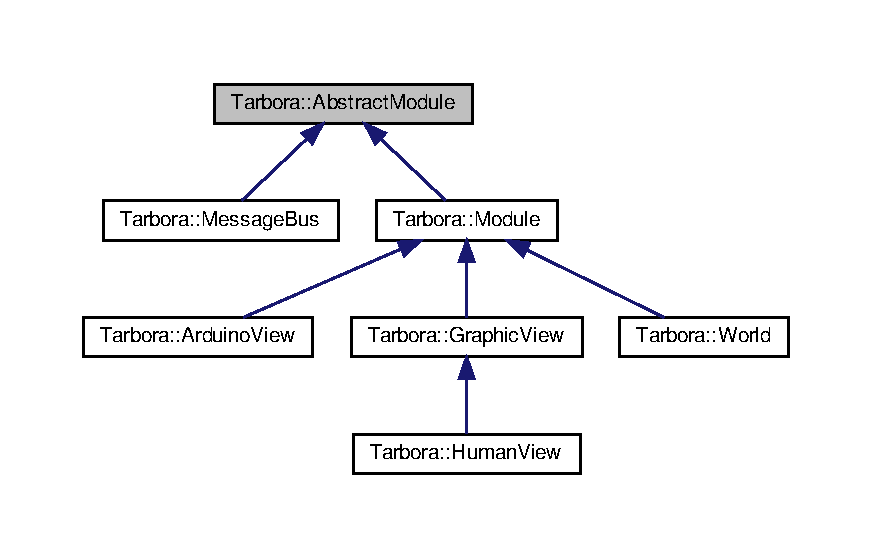
\includegraphics[width=350pt]{classTarbora_1_1AbstractModule__inherit__graph}
\end{center}
\end{figure}
\subsection*{Public Member Functions}
\begin{DoxyCompactItemize}
\item 
virtual void \hyperlink{classTarbora_1_1AbstractModule_acfb70b92b109b5e8ceae997c8629180a}{run} (const std\+::string \&name=\char`\"{}Unamed \hyperlink{classTarbora_1_1Module}{Module}\char`\"{})=0
\begin{DoxyCompactList}\small\item\em Start this module\textquotesingle{}s loop. \end{DoxyCompactList}\item 
void \hyperlink{classTarbora_1_1AbstractModule_ae65c482cc7cca2aae3e24811880c6313}{run\+Thread} (const std\+::string \&name=\char`\"{}Unamed \hyperlink{classTarbora_1_1Module}{Module}\char`\"{})
\begin{DoxyCompactList}\small\item\em Start this module\textquotesingle{}s loop in a new thread. \end{DoxyCompactList}\item 
\mbox{\Hypertarget{classTarbora_1_1AbstractModule_a3b1cc88ec4fc5c1351e5f4abe0e25948}\label{classTarbora_1_1AbstractModule_a3b1cc88ec4fc5c1351e5f4abe0e25948}} 
void \hyperlink{classTarbora_1_1AbstractModule_a3b1cc88ec4fc5c1351e5f4abe0e25948}{close} ()
\begin{DoxyCompactList}\small\item\em Stop this module\textquotesingle{}s loop. \end{DoxyCompactList}\end{DoxyCompactItemize}
\subsection*{Protected Attributes}
\begin{DoxyCompactItemize}
\item 
\mbox{\Hypertarget{classTarbora_1_1AbstractModule_aa13dfaed16573bef7cce22a473616bd5}\label{classTarbora_1_1AbstractModule_aa13dfaed16573bef7cce22a473616bd5}} 
bool {\bfseries using\+\_\+thread\+\_\+}
\end{DoxyCompactItemize}
\subsection*{Static Protected Attributes}
\begin{DoxyCompactItemize}
\item 
\mbox{\Hypertarget{classTarbora_1_1AbstractModule_a66ab779015a191a3188b1f91925e592b}\label{classTarbora_1_1AbstractModule_a66ab779015a191a3188b1f91925e592b}} 
static bool {\bfseries run\+\_\+} = true
\end{DoxyCompactItemize}


\subsection{Detailed Description}
Each of the parts that compose the Engine. 

\subsection{Member Function Documentation}
\mbox{\Hypertarget{classTarbora_1_1AbstractModule_acfb70b92b109b5e8ceae997c8629180a}\label{classTarbora_1_1AbstractModule_acfb70b92b109b5e8ceae997c8629180a}} 
\index{Tarbora\+::\+Abstract\+Module@{Tarbora\+::\+Abstract\+Module}!run@{run}}
\index{run@{run}!Tarbora\+::\+Abstract\+Module@{Tarbora\+::\+Abstract\+Module}}
\subsubsection{\texorpdfstring{run()}{run()}}
{\footnotesize\ttfamily virtual void Tarbora\+::\+Abstract\+Module\+::run (\begin{DoxyParamCaption}\item[{const std\+::string \&}]{name = {\ttfamily \char`\"{}Unamed~\hyperlink{classTarbora_1_1Module}{Module}\char`\"{}} }\end{DoxyParamCaption})\hspace{0.3cm}{\ttfamily [pure virtual]}}



Start this module\textquotesingle{}s loop. 

All modules should stop when Abstract\+Module\+::run\+\_\+ is set to false. 
\begin{DoxyParams}{Parameters}
{\em name} & The name of the module, only used for the profiler. \\
\hline
\end{DoxyParams}


Implemented in \hyperlink{classTarbora_1_1Module_a8c0352045b21b985d3798caa3190c70b}{Tarbora\+::\+Module}.

\mbox{\Hypertarget{classTarbora_1_1AbstractModule_ae65c482cc7cca2aae3e24811880c6313}\label{classTarbora_1_1AbstractModule_ae65c482cc7cca2aae3e24811880c6313}} 
\index{Tarbora\+::\+Abstract\+Module@{Tarbora\+::\+Abstract\+Module}!run\+Thread@{run\+Thread}}
\index{run\+Thread@{run\+Thread}!Tarbora\+::\+Abstract\+Module@{Tarbora\+::\+Abstract\+Module}}
\subsubsection{\texorpdfstring{run\+Thread()}{runThread()}}
{\footnotesize\ttfamily void Tarbora\+::\+Abstract\+Module\+::run\+Thread (\begin{DoxyParamCaption}\item[{const std\+::string \&}]{name = {\ttfamily \char`\"{}Unamed~\hyperlink{classTarbora_1_1Module}{Module}\char`\"{}} }\end{DoxyParamCaption})}



Start this module\textquotesingle{}s loop in a new thread. 


\begin{DoxyParams}{Parameters}
{\em name} & The name of the module, only used for the profiler. \\
\hline
\end{DoxyParams}


The documentation for this class was generated from the following files\+:\begin{DoxyCompactItemize}
\item 
Tarbora/\+Framework/\+Module/Abstract\+Module.\+hpp\item 
Tarbora/\+Framework/\+Module/Abstract\+Module.\+cpp\end{DoxyCompactItemize}

\hypertarget{classTarbora_1_1ActorComponent}{}\section{Tarbora\+:\+:Actor\+Component Class Reference}
\label{classTarbora_1_1ActorComponent}\index{Tarbora\+::\+Actor\+Component@{Tarbora\+::\+Actor\+Component}}


Inheritance diagram for Tarbora\+:\+:Actor\+Component\+:\nopagebreak
\begin{figure}[H]
\begin{center}
\leavevmode
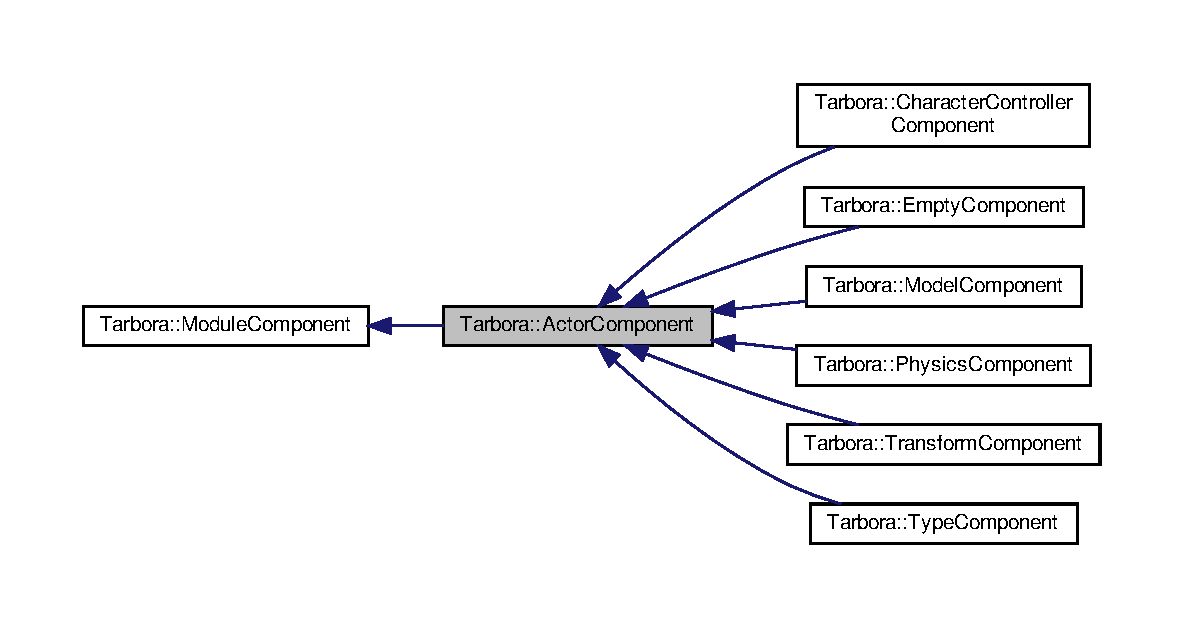
\includegraphics[width=350pt]{classTarbora_1_1ActorComponent__inherit__graph}
\end{center}
\end{figure}


Collaboration diagram for Tarbora\+:\+:Actor\+Component\+:\nopagebreak
\begin{figure}[H]
\begin{center}
\leavevmode
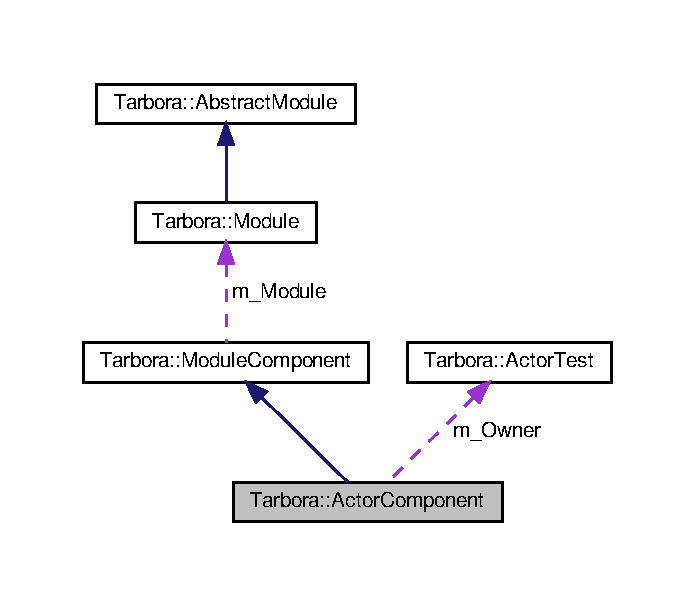
\includegraphics[width=209pt]{classTarbora_1_1ActorComponent__coll__graph}
\end{center}
\end{figure}
\subsection*{Public Member Functions}
\begin{DoxyCompactItemize}
\item 
\mbox{\Hypertarget{classTarbora_1_1ActorComponent_a55d053ca98c31bd3f79f005888b7e428}\label{classTarbora_1_1ActorComponent_a55d053ca98c31bd3f79f005888b7e428}} 
virtual bool {\bfseries Init} (Json\+Ptr resource, raw\+\_\+json data)=0
\item 
\mbox{\Hypertarget{classTarbora_1_1ActorComponent_a940239e984904afe67fc63a70e1be1ec}\label{classTarbora_1_1ActorComponent_a940239e984904afe67fc63a70e1be1ec}} 
virtual void {\bfseries Destroy} ()
\item 
\mbox{\Hypertarget{classTarbora_1_1ActorComponent_ad9139206456b2f466509c35111706b7e}\label{classTarbora_1_1ActorComponent_ad9139206456b2f466509c35111706b7e}} 
virtual void {\bfseries After\+Init} ()
\item 
\mbox{\Hypertarget{classTarbora_1_1ActorComponent_a1819cca7b2392047d95614b2c71cb56e}\label{classTarbora_1_1ActorComponent_a1819cca7b2392047d95614b2c71cb56e}} 
virtual void {\bfseries Update} (float delta\+Time)
\item 
\mbox{\Hypertarget{classTarbora_1_1ActorComponent_a395c55c7c250466e3c037fa4090da5d5}\label{classTarbora_1_1ActorComponent_a395c55c7c250466e3c037fa4090da5d5}} 
virtual Component\+Id {\bfseries Get\+Id} () const =0
\end{DoxyCompactItemize}
\subsection*{Protected Member Functions}
\begin{DoxyCompactItemize}
\item 
\mbox{\Hypertarget{classTarbora_1_1ActorComponent_abf8b7b050e3777624e42336cc661b106}\label{classTarbora_1_1ActorComponent_abf8b7b050e3777624e42336cc661b106}} 
void {\bfseries Set\+Owner} (\hyperlink{classTarbora_1_1ActorTest}{Actor\+Test} $\ast$owner)
\end{DoxyCompactItemize}
\subsection*{Protected Attributes}
\begin{DoxyCompactItemize}
\item 
\mbox{\Hypertarget{classTarbora_1_1ActorComponent_aa1f0c0a35625fe1a16dcb1f0ee67d7e9}\label{classTarbora_1_1ActorComponent_aa1f0c0a35625fe1a16dcb1f0ee67d7e9}} 
\hyperlink{classTarbora_1_1ActorTest}{Actor\+Test} $\ast$ {\bfseries m\+\_\+\+Owner}
\end{DoxyCompactItemize}
\subsection*{Friends}
\begin{DoxyCompactItemize}
\item 
\mbox{\Hypertarget{classTarbora_1_1ActorComponent_a6ab97c7737ba5ca6e4cb3a4621c48421}\label{classTarbora_1_1ActorComponent_a6ab97c7737ba5ca6e4cb3a4621c48421}} 
class {\bfseries Actor\+Factory}
\end{DoxyCompactItemize}


The documentation for this class was generated from the following file\+:\begin{DoxyCompactItemize}
\item 
Tarbora/\+Game\+Logic/inc/Actor\+Component.\+hpp\end{DoxyCompactItemize}

\hypertarget{classTarbora_1_1ActorFactory}{}\section{Tarbora\+:\+:Actor\+Factory Class Reference}
\label{classTarbora_1_1ActorFactory}\index{Tarbora\+::\+Actor\+Factory@{Tarbora\+::\+Actor\+Factory}}
\subsection*{Public Member Functions}
\begin{DoxyCompactItemize}
\item 
\mbox{\Hypertarget{classTarbora_1_1ActorFactory_ac74d6cbd05cc1cd9859baa3c10d08222}\label{classTarbora_1_1ActorFactory_ac74d6cbd05cc1cd9859baa3c10d08222}} 
void {\bfseries Add\+Component\+Creator} (std\+::string name, Actor\+Component\+Creator func)
\item 
\mbox{\Hypertarget{classTarbora_1_1ActorFactory_a2868cc8c4d2a3ea100507e8734084106}\label{classTarbora_1_1ActorFactory_a2868cc8c4d2a3ea100507e8734084106}} 
bool {\bfseries Create} (\hyperlink{classTarbora_1_1ActorTest}{Actor\+Test} $\ast$actor, std\+::string actor\+Resource, glm\+::vec3 initial\+Pos, glm\+::vec3 inital\+Rot)
\end{DoxyCompactItemize}
\subsection*{Protected Member Functions}
\begin{DoxyCompactItemize}
\item 
\mbox{\Hypertarget{classTarbora_1_1ActorFactory_a8716aaffe784609b317b5f30e5724d85}\label{classTarbora_1_1ActorFactory_a8716aaffe784609b317b5f30e5724d85}} 
Actor\+Component\+Ptr {\bfseries Create\+Component} (Json\+Ptr resource, std\+::string name, raw\+\_\+json data)
\end{DoxyCompactItemize}
\subsection*{Protected Attributes}
\begin{DoxyCompactItemize}
\item 
\mbox{\Hypertarget{classTarbora_1_1ActorFactory_afdd824e4b59a45312f5edda0de93cf97}\label{classTarbora_1_1ActorFactory_afdd824e4b59a45312f5edda0de93cf97}} 
Actor\+Component\+Creator\+Map {\bfseries m\+\_\+\+Actor\+Component\+Creators}
\end{DoxyCompactItemize}


The documentation for this class was generated from the following files\+:\begin{DoxyCompactItemize}
\item 
Tarbora/\+Game\+Logic/inc/Actor\+Factory.\+hpp\item 
Tarbora/\+Game\+Logic/src/Actor\+Factory.\+cpp\end{DoxyCompactItemize}

\hypertarget{classTarbora_1_1ActorModel}{}\section{Tarbora\+:\+:Actor\+Model Class Reference}
\label{classTarbora_1_1ActorModel}\index{Tarbora\+::\+Actor\+Model@{Tarbora\+::\+Actor\+Model}}


Inheritance diagram for Tarbora\+:\+:Actor\+Model\+:
\nopagebreak
\begin{figure}[H]
\begin{center}
\leavevmode
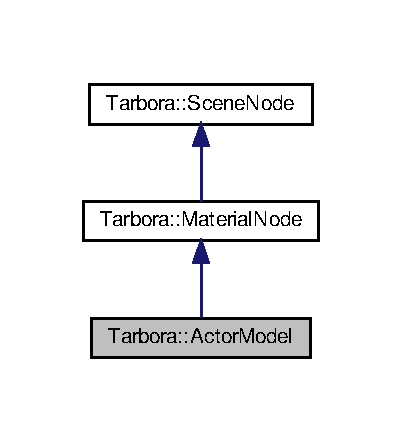
\includegraphics[width=193pt]{classTarbora_1_1ActorModel__inherit__graph}
\end{center}
\end{figure}


Collaboration diagram for Tarbora\+:\+:Actor\+Model\+:
\nopagebreak
\begin{figure}[H]
\begin{center}
\leavevmode
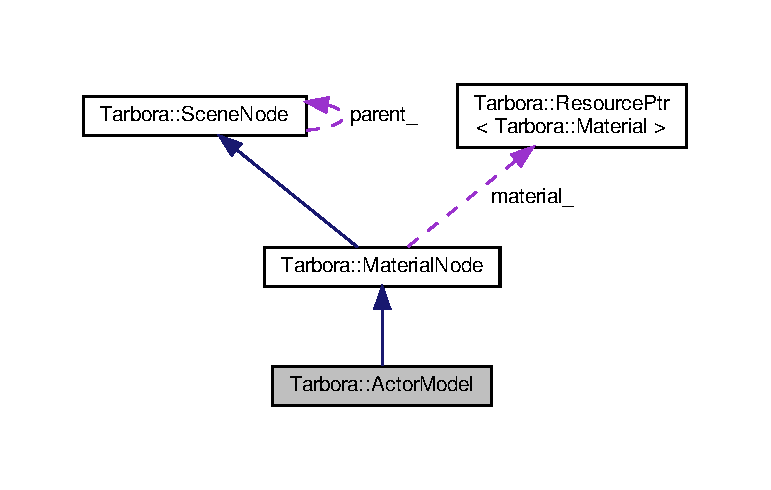
\includegraphics[width=350pt]{classTarbora_1_1ActorModel__coll__graph}
\end{center}
\end{figure}
\subsection*{Public Member Functions}
\begin{DoxyCompactItemize}
\item 
\mbox{\Hypertarget{classTarbora_1_1ActorModel_a1fefe619a840e2bbdf214e5d44962193}\label{classTarbora_1_1ActorModel_a1fefe619a840e2bbdf214e5d44962193}} 
{\bfseries Actor\+Model} (const Actor\+Id \&id, Render\+Pass render\+\_\+pass, const std\+::string \&model, const std\+::string \&material)
\item 
\mbox{\Hypertarget{classTarbora_1_1ActorModel_a444103ab29247d23375fe2a55392fae0}\label{classTarbora_1_1ActorModel_a444103ab29247d23375fe2a55392fae0}} 
std\+::shared\+\_\+ptr$<$ \hyperlink{classTarbora_1_1MeshNode}{Mesh\+Node} $>$ {\bfseries create\+Node} (const Actor\+Id \&id, Render\+Pass render\+\_\+pass, \hyperlink{classTarbora_1_1LuaTable}{Lua\+Table} table)
\item 
\mbox{\Hypertarget{classTarbora_1_1ActorModel_a162b40dc0f465add232c332fd7899610}\label{classTarbora_1_1ActorModel_a162b40dc0f465add232c332fd7899610}} 
std\+::shared\+\_\+ptr$<$ \hyperlink{classTarbora_1_1Camera}{Camera} $>$ {\bfseries create\+Camera} (const Actor\+Id \&id, \hyperlink{classTarbora_1_1LuaTable}{Lua\+Table} table)
\item 
\mbox{\Hypertarget{classTarbora_1_1ActorModel_a7c6a17305abb923b03a190e90b4f856e}\label{classTarbora_1_1ActorModel_a7c6a17305abb923b03a190e90b4f856e}} 
virtual void {\bfseries update} (\hyperlink{classTarbora_1_1Scene}{Scene} $\ast$scene, float delta\+\_\+time) override
\item 
\mbox{\Hypertarget{classTarbora_1_1ActorModel_a896fc0026eeed7a5527846711364cd88}\label{classTarbora_1_1ActorModel_a896fc0026eeed7a5527846711364cd88}} 
virtual std\+::shared\+\_\+ptr$<$ \hyperlink{classTarbora_1_1SceneNode}{Scene\+Node} $>$ {\bfseries get\+Child} (const std\+::string \&name) override
\item 
\mbox{\Hypertarget{classTarbora_1_1ActorModel_ae6ddda6bd0f911223020741eaa0e7694}\label{classTarbora_1_1ActorModel_ae6ddda6bd0f911223020741eaa0e7694}} 
void {\bfseries animate} (const std\+::string \&name, const std\+::string \&file=\char`\"{}\char`\"{})
\item 
\mbox{\Hypertarget{classTarbora_1_1ActorModel_a9c2a219815c5952de9aa1b4cd298b23d}\label{classTarbora_1_1ActorModel_a9c2a219815c5952de9aa1b4cd298b23d}} 
const std\+::string \& {\bfseries get\+Model} ()
\item 
\mbox{\Hypertarget{classTarbora_1_1ActorModel_a2955e28f4e1ab4fcb81affcbcd04cbd5}\label{classTarbora_1_1ActorModel_a2955e28f4e1ab4fcb81affcbcd04cbd5}} 
Render\+Pass {\bfseries get\+Render\+Pass} ()
\end{DoxyCompactItemize}
\subsection*{Friends}
\begin{DoxyCompactItemize}
\item 
\mbox{\Hypertarget{classTarbora_1_1ActorModel_a7899599edce4988a894c8e7431e7bb85}\label{classTarbora_1_1ActorModel_a7899599edce4988a894c8e7431e7bb85}} 
class {\bfseries Animation\+Controller}
\end{DoxyCompactItemize}
\subsection*{Additional Inherited Members}


The documentation for this class was generated from the following files\+:\begin{DoxyCompactItemize}
\item 
Tarbora/\+Views/\+Graphic\+Views/Actor\+Model.\+hpp\item 
Tarbora/\+Views/\+Graphic\+Views/Actor\+Model.\+cpp\end{DoxyCompactItemize}

\hypertarget{classTarbora_1_1ActorMotionState}{}\section{Tarbora\+:\+:Actor\+Motion\+State Class Reference}
\label{classTarbora_1_1ActorMotionState}\index{Tarbora\+::\+Actor\+Motion\+State@{Tarbora\+::\+Actor\+Motion\+State}}


Inheritance diagram for Tarbora\+:\+:Actor\+Motion\+State\+:\nopagebreak
\begin{figure}[H]
\begin{center}
\leavevmode
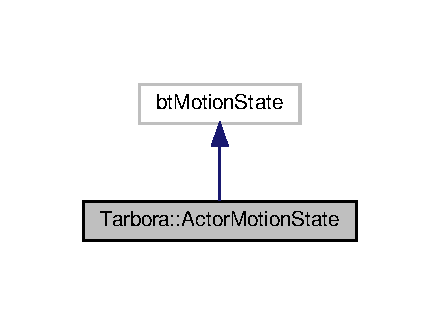
\includegraphics[width=211pt]{classTarbora_1_1ActorMotionState__inherit__graph}
\end{center}
\end{figure}


Collaboration diagram for Tarbora\+:\+:Actor\+Motion\+State\+:\nopagebreak
\begin{figure}[H]
\begin{center}
\leavevmode
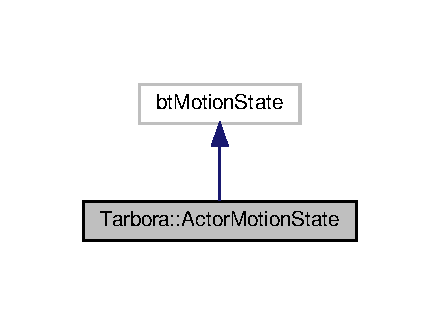
\includegraphics[width=211pt]{classTarbora_1_1ActorMotionState__coll__graph}
\end{center}
\end{figure}
\subsection*{Public Member Functions}
\begin{DoxyCompactItemize}
\item 
\mbox{\Hypertarget{classTarbora_1_1ActorMotionState_a9f0f8dfe3b52a74c0dff5196629f28c9}\label{classTarbora_1_1ActorMotionState_a9f0f8dfe3b52a74c0dff5196629f28c9}} 
{\bfseries Actor\+Motion\+State} (glm\+::mat4 const \&transform)
\item 
\mbox{\Hypertarget{classTarbora_1_1ActorMotionState_a6ca1b1961e95b7469e9dbef6d32f38e4}\label{classTarbora_1_1ActorMotionState_a6ca1b1961e95b7469e9dbef6d32f38e4}} 
virtual void {\bfseries get\+World\+Transform} (bt\+Transform \&transform) const
\item 
\mbox{\Hypertarget{classTarbora_1_1ActorMotionState_a116151bb38d94aede50f35841bb03e6b}\label{classTarbora_1_1ActorMotionState_a116151bb38d94aede50f35841bb03e6b}} 
virtual void {\bfseries set\+World\+Transform} (const bt\+Transform \&transform)
\item 
\mbox{\Hypertarget{classTarbora_1_1ActorMotionState_aebdbbe65dc6e5b8826cc500baf5f0318}\label{classTarbora_1_1ActorMotionState_aebdbbe65dc6e5b8826cc500baf5f0318}} 
void {\bfseries get\+World\+Transform} (glm\+::mat4 \&transform) const
\item 
\mbox{\Hypertarget{classTarbora_1_1ActorMotionState_ac39c57708b091d92a0812f9cda68e7bb}\label{classTarbora_1_1ActorMotionState_ac39c57708b091d92a0812f9cda68e7bb}} 
void {\bfseries set\+World\+Transform} (const glm\+::mat4 \&transform)
\item 
\mbox{\Hypertarget{classTarbora_1_1ActorMotionState_ab79ee121003e3adda3c77c210dadc058}\label{classTarbora_1_1ActorMotionState_ab79ee121003e3adda3c77c210dadc058}} 
glm\+::vec3 {\bfseries get\+Position} ()
\item 
\mbox{\Hypertarget{classTarbora_1_1ActorMotionState_af57e028d47be8d142a01c61c25952eb0}\label{classTarbora_1_1ActorMotionState_af57e028d47be8d142a01c61c25952eb0}} 
glm\+::mat3 {\bfseries get\+Rotation} ()
\end{DoxyCompactItemize}
\subsection*{Public Attributes}
\begin{DoxyCompactItemize}
\item 
\mbox{\Hypertarget{classTarbora_1_1ActorMotionState_a89476c358757187de24d4917f4986b93}\label{classTarbora_1_1ActorMotionState_a89476c358757187de24d4917f4986b93}} 
glm\+::mat4 {\bfseries m\+\_\+\+Transform}
\end{DoxyCompactItemize}


The documentation for this class was generated from the following files\+:\begin{DoxyCompactItemize}
\item 
Tarbora/\+Framework/\+Physics\+Engine/inc/Physics\+Engine.\+hpp\item 
Tarbora/\+Framework/\+Physics\+Engine/src/Physics\+Engine.\+cpp\end{DoxyCompactItemize}

\hypertarget{classTarbora_1_1ActorTest}{}\section{Tarbora\+:\+:Actor\+Test Class Reference}
\label{classTarbora_1_1ActorTest}\index{Tarbora\+::\+Actor\+Test@{Tarbora\+::\+Actor\+Test}}
\subsection*{Public Member Functions}
\begin{DoxyCompactItemize}
\item 
\mbox{\Hypertarget{classTarbora_1_1ActorTest_ad457e844af597ea30074df91d60d628c}\label{classTarbora_1_1ActorTest_ad457e844af597ea30074df91d60d628c}} 
{\bfseries Actor\+Test} (Actor\+Id id)
\item 
\mbox{\Hypertarget{classTarbora_1_1ActorTest_af2567777db6e4d75c021a8df4b253a1b}\label{classTarbora_1_1ActorTest_af2567777db6e4d75c021a8df4b253a1b}} 
bool {\bfseries Init} (Json\+Ptr resource)
\item 
\mbox{\Hypertarget{classTarbora_1_1ActorTest_ad2e97ec6385c50cfb66078bdcc5d952d}\label{classTarbora_1_1ActorTest_ad2e97ec6385c50cfb66078bdcc5d952d}} 
void {\bfseries After\+Init} ()
\item 
\mbox{\Hypertarget{classTarbora_1_1ActorTest_a21c45d268e7d3a8f4f6fc059d8d66a92}\label{classTarbora_1_1ActorTest_a21c45d268e7d3a8f4f6fc059d8d66a92}} 
void {\bfseries Destroy} ()
\item 
\mbox{\Hypertarget{classTarbora_1_1ActorTest_a363465e2cc6e35bc8a6d8fce27a132e1}\label{classTarbora_1_1ActorTest_a363465e2cc6e35bc8a6d8fce27a132e1}} 
void {\bfseries Update} (float delta\+Time)
\item 
\mbox{\Hypertarget{classTarbora_1_1ActorTest_a5c561bad40317d007cc45e9857341c13}\label{classTarbora_1_1ActorTest_a5c561bad40317d007cc45e9857341c13}} 
Actor\+Id {\bfseries Get\+Id} () const
\item 
\mbox{\Hypertarget{classTarbora_1_1ActorTest_aba485020e32f40d814aa9573d540de73}\label{classTarbora_1_1ActorTest_aba485020e32f40d814aa9573d540de73}} 
Actor\+Component\+Ptr {\bfseries Get\+Component} (Component\+Id id)
\item 
\mbox{\Hypertarget{classTarbora_1_1ActorTest_a98299208ea87526838a5f218e28cd447}\label{classTarbora_1_1ActorTest_a98299208ea87526838a5f218e28cd447}} 
\hyperlink{classTarbora_1_1ActorTest}{Actor\+Test} $\ast$ {\bfseries Get\+Next} () const
\item 
\mbox{\Hypertarget{classTarbora_1_1ActorTest_affe274cb45db8c34aa7edc562964a678}\label{classTarbora_1_1ActorTest_affe274cb45db8c34aa7edc562964a678}} 
void {\bfseries Set\+Next} (\hyperlink{classTarbora_1_1ActorTest}{Actor\+Test} $\ast$next)
\end{DoxyCompactItemize}
\subsection*{Friends}
\begin{DoxyCompactItemize}
\item 
\mbox{\Hypertarget{classTarbora_1_1ActorTest_a6ab97c7737ba5ca6e4cb3a4621c48421}\label{classTarbora_1_1ActorTest_a6ab97c7737ba5ca6e4cb3a4621c48421}} 
class {\bfseries Actor\+Factory}
\item 
\mbox{\Hypertarget{classTarbora_1_1ActorTest_ae2bbe52c24cb66e52b1c2066fe9eccc9}\label{classTarbora_1_1ActorTest_ae2bbe52c24cb66e52b1c2066fe9eccc9}} 
class {\bfseries Actors}
\end{DoxyCompactItemize}


The documentation for this class was generated from the following files\+:\begin{DoxyCompactItemize}
\item 
Tarbora/\+Game\+Logic/inc/Actor.\+hpp\item 
Tarbora/\+Game\+Logic/src/Actor.\+cpp\end{DoxyCompactItemize}

\hypertarget{classTarbora_1_1AnimationController}{}\section{Tarbora\+:\+:Animation\+Controller Class Reference}
\label{classTarbora_1_1AnimationController}\index{Tarbora\+::\+Animation\+Controller@{Tarbora\+::\+Animation\+Controller}}
\subsection*{Public Member Functions}
\begin{DoxyCompactItemize}
\item 
\mbox{\Hypertarget{classTarbora_1_1AnimationController_a3646c4571530d81d0b0dc58e0aab08fe}\label{classTarbora_1_1AnimationController_a3646c4571530d81d0b0dc58e0aab08fe}} 
{\bfseries Animation\+Controller} (\hyperlink{classTarbora_1_1ActorModel}{Actor\+Model} $\ast$actor, std\+::string animations\+\_\+file)
\item 
\mbox{\Hypertarget{classTarbora_1_1AnimationController_a5e16fba3e32db6e6ac061a54ae9949b1}\label{classTarbora_1_1AnimationController_a5e16fba3e32db6e6ac061a54ae9949b1}} 
void {\bfseries Update} (float delta\+Time)
\item 
\mbox{\Hypertarget{classTarbora_1_1AnimationController_a82ebfc6b041c20700252196c7aefc656}\label{classTarbora_1_1AnimationController_a82ebfc6b041c20700252196c7aefc656}} 
void {\bfseries Set\+Animation} (std\+::string animation\+\_\+name)
\item 
\mbox{\Hypertarget{classTarbora_1_1AnimationController_aa5f632bc3c8cea954f083f52d715ccf1}\label{classTarbora_1_1AnimationController_aa5f632bc3c8cea954f083f52d715ccf1}} 
void {\bfseries Update\+Animation} (float frame)
\end{DoxyCompactItemize}


The documentation for this class was generated from the following files\+:\begin{DoxyCompactItemize}
\item 
Tarbora/\+Views/\+Graphic\+Views/inc/Animation\+Controller.\+hpp\item 
Tarbora/\+Views/\+Graphic\+Views/src/Animation\+Controller.\+cpp\end{DoxyCompactItemize}

\hypertarget{classTarbora_1_1ApplyPhysics}{}\section{Tarbora\+:\+:Apply\+Physics Class Reference}
\label{classTarbora_1_1ApplyPhysics}\index{Tarbora\+::\+Apply\+Physics@{Tarbora\+::\+Apply\+Physics}}


Inheritance diagram for Tarbora\+:\+:Apply\+Physics\+:
\nopagebreak
\begin{figure}[H]
\begin{center}
\leavevmode
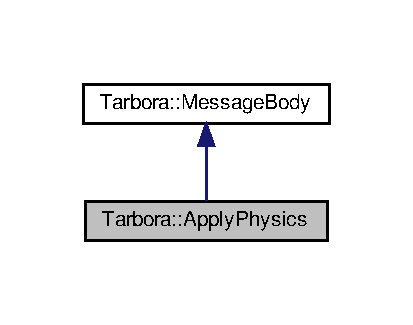
\includegraphics[width=198pt]{classTarbora_1_1ApplyPhysics__inherit__graph}
\end{center}
\end{figure}


Collaboration diagram for Tarbora\+:\+:Apply\+Physics\+:
\nopagebreak
\begin{figure}[H]
\begin{center}
\leavevmode
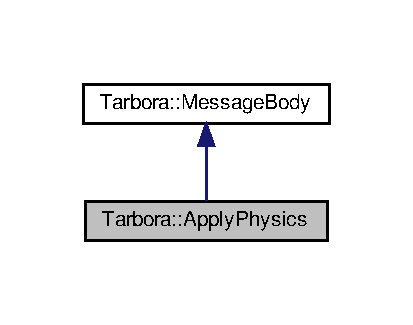
\includegraphics[width=198pt]{classTarbora_1_1ApplyPhysics__coll__graph}
\end{center}
\end{figure}
\subsection*{Public Member Functions}
\begin{DoxyCompactItemize}
\item 
\mbox{\Hypertarget{classTarbora_1_1ApplyPhysics_af65460192f54355105775681a41fbc1f}\label{classTarbora_1_1ApplyPhysics_af65460192f54355105775681a41fbc1f}} 
{\bfseries Apply\+Physics} (unsigned int id, float magnitude, glm\+::vec3 direction)
\end{DoxyCompactItemize}
\subsection*{Additional Inherited Members}


The documentation for this class was generated from the following file\+:\begin{DoxyCompactItemize}
\item 
Tarbora/\+Messages/Basic\+Messages.\+hpp\end{DoxyCompactItemize}

\hypertarget{classtbBasics_1_1ApplyPhysicsBody}{}\section{tb\+Basics\+:\+:Apply\+Physics\+Body Class Reference}
\label{classtbBasics_1_1ApplyPhysicsBody}\index{tb\+Basics\+::\+Apply\+Physics\+Body@{tb\+Basics\+::\+Apply\+Physics\+Body}}


Inheritance diagram for tb\+Basics\+:\+:Apply\+Physics\+Body\+:
\nopagebreak
\begin{figure}[H]
\begin{center}
\leavevmode
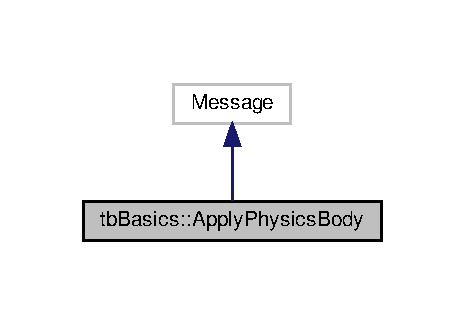
\includegraphics[width=223pt]{classtbBasics_1_1ApplyPhysicsBody__inherit__graph}
\end{center}
\end{figure}


Collaboration diagram for tb\+Basics\+:\+:Apply\+Physics\+Body\+:
\nopagebreak
\begin{figure}[H]
\begin{center}
\leavevmode
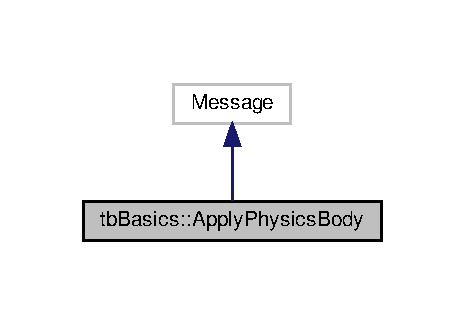
\includegraphics[width=223pt]{classtbBasics_1_1ApplyPhysicsBody__coll__graph}
\end{center}
\end{figure}
\subsection*{Classes}
\begin{DoxyCompactItemize}
\item 
class \hyperlink{classtbBasics_1_1ApplyPhysicsBody_1_1HasBitSetters}{Has\+Bit\+Setters}
\end{DoxyCompactItemize}
\subsection*{Public Member Functions}
\begin{DoxyCompactItemize}
\item 
\mbox{\Hypertarget{classtbBasics_1_1ApplyPhysicsBody_a433051e19a2465744f2eba4397206cd0}\label{classtbBasics_1_1ApplyPhysicsBody_a433051e19a2465744f2eba4397206cd0}} 
{\bfseries Apply\+Physics\+Body} (const \hyperlink{classtbBasics_1_1ApplyPhysicsBody}{Apply\+Physics\+Body} \&from)
\item 
\mbox{\Hypertarget{classtbBasics_1_1ApplyPhysicsBody_a4b80294da46db71cb3a9302d8627efbd}\label{classtbBasics_1_1ApplyPhysicsBody_a4b80294da46db71cb3a9302d8627efbd}} 
\hyperlink{classtbBasics_1_1ApplyPhysicsBody}{Apply\+Physics\+Body} \& {\bfseries operator=} (const \hyperlink{classtbBasics_1_1ApplyPhysicsBody}{Apply\+Physics\+Body} \&from)
\item 
\mbox{\Hypertarget{classtbBasics_1_1ApplyPhysicsBody_ada3c30bfa3c30a6723050893deb8b793}\label{classtbBasics_1_1ApplyPhysicsBody_ada3c30bfa3c30a6723050893deb8b793}} 
void {\bfseries Swap} (\hyperlink{classtbBasics_1_1ApplyPhysicsBody}{Apply\+Physics\+Body} $\ast$other)
\item 
\mbox{\Hypertarget{classtbBasics_1_1ApplyPhysicsBody_a89af82acb9d6c40bccb167c597d90547}\label{classtbBasics_1_1ApplyPhysicsBody_a89af82acb9d6c40bccb167c597d90547}} 
\hyperlink{classtbBasics_1_1ApplyPhysicsBody}{Apply\+Physics\+Body} $\ast$ {\bfseries New} () const final
\item 
\mbox{\Hypertarget{classtbBasics_1_1ApplyPhysicsBody_ae87da4e97dcdd4c8ff79045d39b0c47e}\label{classtbBasics_1_1ApplyPhysicsBody_ae87da4e97dcdd4c8ff79045d39b0c47e}} 
\hyperlink{classtbBasics_1_1ApplyPhysicsBody}{Apply\+Physics\+Body} $\ast$ {\bfseries New} (\+::google\+::protobuf\+::\+Arena $\ast$arena) const final
\item 
\mbox{\Hypertarget{classtbBasics_1_1ApplyPhysicsBody_a352ff64aafa11ca600e6ded25c4e6ff8}\label{classtbBasics_1_1ApplyPhysicsBody_a352ff64aafa11ca600e6ded25c4e6ff8}} 
void {\bfseries Copy\+From} (const \+::google\+::protobuf\+::\+Message \&from) final
\item 
\mbox{\Hypertarget{classtbBasics_1_1ApplyPhysicsBody_a99c0a8df25fb94d563141251c74508e9}\label{classtbBasics_1_1ApplyPhysicsBody_a99c0a8df25fb94d563141251c74508e9}} 
void {\bfseries Merge\+From} (const \+::google\+::protobuf\+::\+Message \&from) final
\item 
\mbox{\Hypertarget{classtbBasics_1_1ApplyPhysicsBody_abc2b1042706a816897980de3e477436a}\label{classtbBasics_1_1ApplyPhysicsBody_abc2b1042706a816897980de3e477436a}} 
void {\bfseries Copy\+From} (const \hyperlink{classtbBasics_1_1ApplyPhysicsBody}{Apply\+Physics\+Body} \&from)
\item 
\mbox{\Hypertarget{classtbBasics_1_1ApplyPhysicsBody_a3a7739c14fab1ecc3e4092bc371c6a8e}\label{classtbBasics_1_1ApplyPhysicsBody_a3a7739c14fab1ecc3e4092bc371c6a8e}} 
void {\bfseries Merge\+From} (const \hyperlink{classtbBasics_1_1ApplyPhysicsBody}{Apply\+Physics\+Body} \&from)
\item 
\mbox{\Hypertarget{classtbBasics_1_1ApplyPhysicsBody_ac86fcdd446551a87e1e528672d5131eb}\label{classtbBasics_1_1ApplyPhysicsBody_ac86fcdd446551a87e1e528672d5131eb}} 
P\+R\+O\+T\+O\+B\+U\+F\+\_\+\+A\+T\+T\+R\+I\+B\+U\+T\+E\+\_\+\+R\+E\+I\+N\+I\+T\+I\+A\+L\+I\+Z\+ES void {\bfseries Clear} () final
\item 
\mbox{\Hypertarget{classtbBasics_1_1ApplyPhysicsBody_a1dd87b948e871d43251808aca0bfacab}\label{classtbBasics_1_1ApplyPhysicsBody_a1dd87b948e871d43251808aca0bfacab}} 
bool {\bfseries Is\+Initialized} () const final
\item 
\mbox{\Hypertarget{classtbBasics_1_1ApplyPhysicsBody_a3212c8a84d585ca507ff4ac48507d778}\label{classtbBasics_1_1ApplyPhysicsBody_a3212c8a84d585ca507ff4ac48507d778}} 
size\+\_\+t {\bfseries Byte\+Size\+Long} () const final
\item 
\mbox{\Hypertarget{classtbBasics_1_1ApplyPhysicsBody_a44acb53a119a391937bfe7de0a27381f}\label{classtbBasics_1_1ApplyPhysicsBody_a44acb53a119a391937bfe7de0a27381f}} 
bool {\bfseries Merge\+Partial\+From\+Coded\+Stream} (\+::google\+::protobuf\+::io\+::\+Coded\+Input\+Stream $\ast$input) final
\item 
\mbox{\Hypertarget{classtbBasics_1_1ApplyPhysicsBody_a260a51ed152f6848a9d51bf0e8258884}\label{classtbBasics_1_1ApplyPhysicsBody_a260a51ed152f6848a9d51bf0e8258884}} 
void {\bfseries Serialize\+With\+Cached\+Sizes} (\+::google\+::protobuf\+::io\+::\+Coded\+Output\+Stream $\ast$output) const final
\item 
\mbox{\Hypertarget{classtbBasics_1_1ApplyPhysicsBody_a793064d6de829a5ea371764a4a2a5b27}\label{classtbBasics_1_1ApplyPhysicsBody_a793064d6de829a5ea371764a4a2a5b27}} 
\+::google\+::protobuf\+::uint8 $\ast$ {\bfseries Internal\+Serialize\+With\+Cached\+Sizes\+To\+Array} (\+::google\+::protobuf\+::uint8 $\ast$target) const final
\item 
\mbox{\Hypertarget{classtbBasics_1_1ApplyPhysicsBody_ac26b0cf6739699e2a33d6ddd1c937776}\label{classtbBasics_1_1ApplyPhysicsBody_ac26b0cf6739699e2a33d6ddd1c937776}} 
int {\bfseries Get\+Cached\+Size} () const final
\item 
\mbox{\Hypertarget{classtbBasics_1_1ApplyPhysicsBody_a2d844208c01cb19710e0226d0ef976a1}\label{classtbBasics_1_1ApplyPhysicsBody_a2d844208c01cb19710e0226d0ef976a1}} 
\+::google\+::protobuf\+::\+Metadata {\bfseries Get\+Metadata} () const final
\item 
\mbox{\Hypertarget{classtbBasics_1_1ApplyPhysicsBody_a1a2f2dc3459a646cfb0b2ac9e08d12e8}\label{classtbBasics_1_1ApplyPhysicsBody_a1a2f2dc3459a646cfb0b2ac9e08d12e8}} 
bool {\bfseries has\+\_\+direction} () const
\item 
\mbox{\Hypertarget{classtbBasics_1_1ApplyPhysicsBody_a9a8a63176c8be83bf9a5754ffb4c842f}\label{classtbBasics_1_1ApplyPhysicsBody_a9a8a63176c8be83bf9a5754ffb4c842f}} 
void {\bfseries clear\+\_\+direction} ()
\item 
\mbox{\Hypertarget{classtbBasics_1_1ApplyPhysicsBody_a36e6926c8012d4de6907728b8d406ccb}\label{classtbBasics_1_1ApplyPhysicsBody_a36e6926c8012d4de6907728b8d406ccb}} 
const \+::\hyperlink{classtbMath_1_1Vec3Message}{tb\+Math\+::\+Vec3\+Message} \& {\bfseries direction} () const
\item 
\mbox{\Hypertarget{classtbBasics_1_1ApplyPhysicsBody_a75e4c5908badb5cb659d190b9b8971bc}\label{classtbBasics_1_1ApplyPhysicsBody_a75e4c5908badb5cb659d190b9b8971bc}} 
\+::\hyperlink{classtbMath_1_1Vec3Message}{tb\+Math\+::\+Vec3\+Message} $\ast$ {\bfseries release\+\_\+direction} ()
\item 
\mbox{\Hypertarget{classtbBasics_1_1ApplyPhysicsBody_aed5a00b3af4172f15c728c2c6d9be782}\label{classtbBasics_1_1ApplyPhysicsBody_aed5a00b3af4172f15c728c2c6d9be782}} 
\+::\hyperlink{classtbMath_1_1Vec3Message}{tb\+Math\+::\+Vec3\+Message} $\ast$ {\bfseries mutable\+\_\+direction} ()
\item 
\mbox{\Hypertarget{classtbBasics_1_1ApplyPhysicsBody_a6556de2b398a9764f92543a2afbce199}\label{classtbBasics_1_1ApplyPhysicsBody_a6556de2b398a9764f92543a2afbce199}} 
void {\bfseries set\+\_\+allocated\+\_\+direction} (\+::\hyperlink{classtbMath_1_1Vec3Message}{tb\+Math\+::\+Vec3\+Message} $\ast$direction)
\item 
\mbox{\Hypertarget{classtbBasics_1_1ApplyPhysicsBody_ac373c7ab9ab74b78c6b9f484f6e4281d}\label{classtbBasics_1_1ApplyPhysicsBody_ac373c7ab9ab74b78c6b9f484f6e4281d}} 
void {\bfseries clear\+\_\+id} ()
\item 
\mbox{\Hypertarget{classtbBasics_1_1ApplyPhysicsBody_ad1c65cd8d6f7b8b2506c6c3b69030316}\label{classtbBasics_1_1ApplyPhysicsBody_ad1c65cd8d6f7b8b2506c6c3b69030316}} 
\+::google\+::protobuf\+::uint32 {\bfseries id} () const
\item 
\mbox{\Hypertarget{classtbBasics_1_1ApplyPhysicsBody_a3622c8051c8ad889f98caa0066ba3232}\label{classtbBasics_1_1ApplyPhysicsBody_a3622c8051c8ad889f98caa0066ba3232}} 
void {\bfseries set\+\_\+id} (\+::google\+::protobuf\+::uint32 value)
\item 
\mbox{\Hypertarget{classtbBasics_1_1ApplyPhysicsBody_abe4eaf91d3d71c9c2b91256646088fe4}\label{classtbBasics_1_1ApplyPhysicsBody_abe4eaf91d3d71c9c2b91256646088fe4}} 
void {\bfseries clear\+\_\+magnitude} ()
\item 
\mbox{\Hypertarget{classtbBasics_1_1ApplyPhysicsBody_af9ea486ab09fef38b5a68bd929d5d67e}\label{classtbBasics_1_1ApplyPhysicsBody_af9ea486ab09fef38b5a68bd929d5d67e}} 
float {\bfseries magnitude} () const
\item 
\mbox{\Hypertarget{classtbBasics_1_1ApplyPhysicsBody_a205189469c5267768fef540a1ce38ccf}\label{classtbBasics_1_1ApplyPhysicsBody_a205189469c5267768fef540a1ce38ccf}} 
void {\bfseries set\+\_\+magnitude} (float value)
\end{DoxyCompactItemize}
\subsection*{Static Public Member Functions}
\begin{DoxyCompactItemize}
\item 
\mbox{\Hypertarget{classtbBasics_1_1ApplyPhysicsBody_aed11b34842b8bdd9efb5e6ae787d5433}\label{classtbBasics_1_1ApplyPhysicsBody_aed11b34842b8bdd9efb5e6ae787d5433}} 
static const \+::google\+::protobuf\+::\+Descriptor $\ast$ {\bfseries descriptor} ()
\item 
\mbox{\Hypertarget{classtbBasics_1_1ApplyPhysicsBody_aa5d64c13e3c27fa45af3ea8d095c2738}\label{classtbBasics_1_1ApplyPhysicsBody_aa5d64c13e3c27fa45af3ea8d095c2738}} 
static const \hyperlink{classtbBasics_1_1ApplyPhysicsBody}{Apply\+Physics\+Body} \& {\bfseries default\+\_\+instance} ()
\item 
\mbox{\Hypertarget{classtbBasics_1_1ApplyPhysicsBody_aa8e8a71f01ce92c86d4447e6dabfcece}\label{classtbBasics_1_1ApplyPhysicsBody_aa8e8a71f01ce92c86d4447e6dabfcece}} 
static void {\bfseries Init\+As\+Default\+Instance} ()
\item 
\mbox{\Hypertarget{classtbBasics_1_1ApplyPhysicsBody_a1e7389e7c6ebc417e82f62ea5133a477}\label{classtbBasics_1_1ApplyPhysicsBody_a1e7389e7c6ebc417e82f62ea5133a477}} 
static const \hyperlink{classtbBasics_1_1ApplyPhysicsBody}{Apply\+Physics\+Body} $\ast$ {\bfseries internal\+\_\+default\+\_\+instance} ()
\end{DoxyCompactItemize}
\subsection*{Static Public Attributes}
\begin{DoxyCompactItemize}
\item 
static constexpr int {\bfseries k\+Index\+In\+File\+Messages}
\item 
\mbox{\Hypertarget{classtbBasics_1_1ApplyPhysicsBody_a794a498a3d705c91852bed8ab112f620}\label{classtbBasics_1_1ApplyPhysicsBody_a794a498a3d705c91852bed8ab112f620}} 
static const int {\bfseries k\+Direction\+Field\+Number} = 3
\item 
\mbox{\Hypertarget{classtbBasics_1_1ApplyPhysicsBody_a8db848cb7b1f73589bdf407f46538ea8}\label{classtbBasics_1_1ApplyPhysicsBody_a8db848cb7b1f73589bdf407f46538ea8}} 
static const int {\bfseries k\+Id\+Field\+Number} = 1
\item 
\mbox{\Hypertarget{classtbBasics_1_1ApplyPhysicsBody_a755bd5beedfeadb318505885c9b70c6a}\label{classtbBasics_1_1ApplyPhysicsBody_a755bd5beedfeadb318505885c9b70c6a}} 
static const int {\bfseries k\+Magnitude\+Field\+Number} = 2
\end{DoxyCompactItemize}
\subsection*{Friends}
\begin{DoxyCompactItemize}
\item 
\mbox{\Hypertarget{classtbBasics_1_1ApplyPhysicsBody_ae86a2f4c520666b65d606ccbe2122e61}\label{classtbBasics_1_1ApplyPhysicsBody_ae86a2f4c520666b65d606ccbe2122e61}} 
struct {\bfseries \+::\+Table\+Struct\+\_\+basic\+\_\+2eproto}
\item 
\mbox{\Hypertarget{classtbBasics_1_1ApplyPhysicsBody_adb9d7c13a818cb90212c6cb502ef9a16}\label{classtbBasics_1_1ApplyPhysicsBody_adb9d7c13a818cb90212c6cb502ef9a16}} 
void {\bfseries swap} (\hyperlink{classtbBasics_1_1ApplyPhysicsBody}{Apply\+Physics\+Body} \&a, \hyperlink{classtbBasics_1_1ApplyPhysicsBody}{Apply\+Physics\+Body} \&b)
\end{DoxyCompactItemize}


\subsection{Member Data Documentation}
\mbox{\Hypertarget{classtbBasics_1_1ApplyPhysicsBody_a012f138363740aef47b3c3be5dd8f8d9}\label{classtbBasics_1_1ApplyPhysicsBody_a012f138363740aef47b3c3be5dd8f8d9}} 
\index{tb\+Basics\+::\+Apply\+Physics\+Body@{tb\+Basics\+::\+Apply\+Physics\+Body}!k\+Index\+In\+File\+Messages@{k\+Index\+In\+File\+Messages}}
\index{k\+Index\+In\+File\+Messages@{k\+Index\+In\+File\+Messages}!tb\+Basics\+::\+Apply\+Physics\+Body@{tb\+Basics\+::\+Apply\+Physics\+Body}}
\subsubsection{\texorpdfstring{k\+Index\+In\+File\+Messages}{kIndexInFileMessages}}
{\footnotesize\ttfamily constexpr int tb\+Basics\+::\+Apply\+Physics\+Body\+::k\+Index\+In\+File\+Messages\hspace{0.3cm}{\ttfamily [static]}}

{\bfseries Initial value\+:}
\begin{DoxyCode}
=
    5
\end{DoxyCode}


The documentation for this class was generated from the following files\+:\begin{DoxyCompactItemize}
\item 
Tarbora/\+Messages/proto/basic.\+pb.\+h\item 
Tarbora/\+Messages/proto/basic.\+pb.\+cc\end{DoxyCompactItemize}

\hypertarget{classtbBasics_1_1ApplyPhysicsBodyDefaultTypeInternal}{}\section{tb\+Basics\+:\+:Apply\+Physics\+Body\+Default\+Type\+Internal Class Reference}
\label{classtbBasics_1_1ApplyPhysicsBodyDefaultTypeInternal}\index{tb\+Basics\+::\+Apply\+Physics\+Body\+Default\+Type\+Internal@{tb\+Basics\+::\+Apply\+Physics\+Body\+Default\+Type\+Internal}}
\subsection*{Public Attributes}
\begin{DoxyCompactItemize}
\item 
\mbox{\Hypertarget{classtbBasics_1_1ApplyPhysicsBodyDefaultTypeInternal_a8bfcdf4b6f23a98a324972fe16266a42}\label{classtbBasics_1_1ApplyPhysicsBodyDefaultTypeInternal_a8bfcdf4b6f23a98a324972fe16266a42}} 
\+::google\+::protobuf\+::internal\+::\+Explicitly\+Constructed$<$ \hyperlink{classtbBasics_1_1ApplyPhysicsBody}{Apply\+Physics\+Body} $>$ {\bfseries \+\_\+instance}
\end{DoxyCompactItemize}


The documentation for this class was generated from the following file\+:\begin{DoxyCompactItemize}
\item 
Tarbora/\+Messages/proto/basic.\+pb.\+cc\end{DoxyCompactItemize}

\hypertarget{classTarbora_1_1ArduinoView}{}\section{Tarbora\+:\+:Arduino\+View Class Reference}
\label{classTarbora_1_1ArduinoView}\index{Tarbora\+::\+Arduino\+View@{Tarbora\+::\+Arduino\+View}}


Inheritance diagram for Tarbora\+:\+:Arduino\+View\+:\nopagebreak
\begin{figure}[H]
\begin{center}
\leavevmode
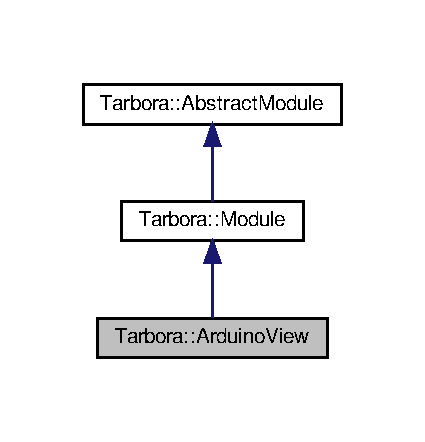
\includegraphics[width=204pt]{classTarbora_1_1ArduinoView__inherit__graph}
\end{center}
\end{figure}


Collaboration diagram for Tarbora\+:\+:Arduino\+View\+:\nopagebreak
\begin{figure}[H]
\begin{center}
\leavevmode
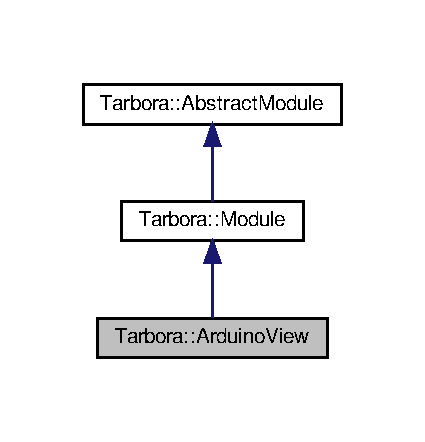
\includegraphics[width=204pt]{classTarbora_1_1ArduinoView__coll__graph}
\end{center}
\end{figure}
\subsection*{Public Member Functions}
\begin{DoxyCompactItemize}
\item 
\mbox{\Hypertarget{classTarbora_1_1ArduinoView_a76e2e6d8fc47da1fa28fe75b80a89449}\label{classTarbora_1_1ArduinoView_a76e2e6d8fc47da1fa28fe75b80a89449}} 
virtual void {\bfseries update} (float delta\+\_\+time) override
\end{DoxyCompactItemize}
\subsection*{Additional Inherited Members}


The documentation for this class was generated from the following files\+:\begin{DoxyCompactItemize}
\item 
Tarbora/\+Views/\+Hardware\+Views/inc/Arduino\+View.\+hpp\item 
Tarbora/\+Views/\+Hardware\+Views/src/Arduino\+View.\+cpp\end{DoxyCompactItemize}

\hypertarget{classTarbora_1_1BoxBody}{}\section{Tarbora\+:\+:Box\+Body Class Reference}
\label{classTarbora_1_1BoxBody}\index{Tarbora\+::\+Box\+Body@{Tarbora\+::\+Box\+Body}}


A physics rigid body representing a cube.  




{\ttfamily \#include $<$Rigid\+Body.\+hpp$>$}



Inheritance diagram for Tarbora\+:\+:Box\+Body\+:\nopagebreak
\begin{figure}[H]
\begin{center}
\leavevmode
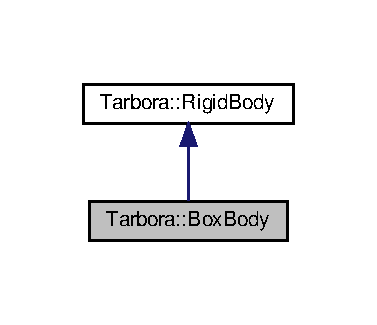
\includegraphics[width=181pt]{classTarbora_1_1BoxBody__inherit__graph}
\end{center}
\end{figure}


Collaboration diagram for Tarbora\+:\+:Box\+Body\+:\nopagebreak
\begin{figure}[H]
\begin{center}
\leavevmode
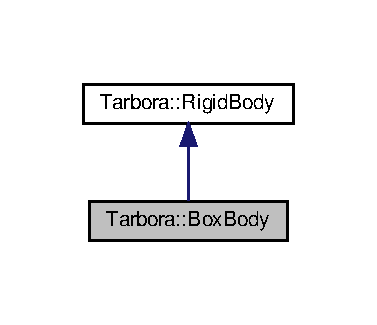
\includegraphics[width=181pt]{classTarbora_1_1BoxBody__coll__graph}
\end{center}
\end{figure}
\subsection*{Public Member Functions}
\begin{DoxyCompactItemize}
\item 
\hyperlink{classTarbora_1_1BoxBody_a4588faa74c221c9f484432bc3b7a0674}{Box\+Body} (glm\+::vec3 \&dimensions)
\begin{DoxyCompactList}\small\item\em Creates a \hyperlink{classTarbora_1_1BoxBody}{Box\+Body}. \end{DoxyCompactList}\item 
\mbox{\Hypertarget{classTarbora_1_1BoxBody_adb0e7074d88a5e14ae8c9abca875ac52}\label{classTarbora_1_1BoxBody_adb0e7074d88a5e14ae8c9abca875ac52}} 
\hyperlink{classTarbora_1_1BoxBody_adb0e7074d88a5e14ae8c9abca875ac52}{$\sim$\+Box\+Body} ()
\begin{DoxyCompactList}\small\item\em Destroys and unregisters this body. \end{DoxyCompactList}\item 
virtual void \hyperlink{classTarbora_1_1BoxBody_a9030e38449087fdf091d9daea5e6efbe}{Register} (unsigned int id, glm\+::mat4 \&transform) override
\begin{DoxyCompactList}\small\item\em Register the rigid body to the Physics Engine. \end{DoxyCompactList}\item 
\mbox{\Hypertarget{classTarbora_1_1BoxBody_a57a94943897a3b90f774935bef82c47c}\label{classTarbora_1_1BoxBody_a57a94943897a3b90f774935bef82c47c}} 
virtual void \hyperlink{classTarbora_1_1BoxBody_a57a94943897a3b90f774935bef82c47c}{Unregister} () override
\begin{DoxyCompactList}\small\item\em Remove the rigid body from the Physics Engine. \end{DoxyCompactList}\item 
\mbox{\Hypertarget{classTarbora_1_1BoxBody_ab5632e04e516e518297a4826c6dd27cb}\label{classTarbora_1_1BoxBody_ab5632e04e516e518297a4826c6dd27cb}} 
virtual void \hyperlink{classTarbora_1_1BoxBody_ab5632e04e516e518297a4826c6dd27cb}{Calc\+Volume} () override
\begin{DoxyCompactList}\small\item\em Calculate the volume when the shape or the size changes. Automatically called by the functions that change those. \end{DoxyCompactList}\item 
void \hyperlink{classTarbora_1_1BoxBody_ae4b822b4acb781e9fdec907e8a92b27b}{Set\+Dimensions} (glm\+::vec3 \&dimensions)
\begin{DoxyCompactList}\small\item\em Set the dimensions of that box, used to calculate the volume and the mass. \end{DoxyCompactList}\item 
\mbox{\Hypertarget{classTarbora_1_1BoxBody_a2c833613435aa7244e39f14460a792c6}\label{classTarbora_1_1BoxBody_a2c833613435aa7244e39f14460a792c6}} 
glm\+::vec3 \& \hyperlink{classTarbora_1_1BoxBody_a2c833613435aa7244e39f14460a792c6}{Get\+Dimensions} ()
\begin{DoxyCompactList}\small\item\em Get the dimensions of that box. \end{DoxyCompactList}\end{DoxyCompactItemize}
\subsection*{Additional Inherited Members}


\subsection{Detailed Description}
A physics rigid body representing a cube. 

\begin{DoxySeeAlso}{See also}
\hyperlink{classTarbora_1_1PhysicsEngine}{Physics\+Engine} 

\hyperlink{classTarbora_1_1RigidBody}{Rigid\+Body} 

\hyperlink{classTarbora_1_1SphereBody}{Sphere\+Body} 
\end{DoxySeeAlso}


\subsection{Constructor \& Destructor Documentation}
\mbox{\Hypertarget{classTarbora_1_1BoxBody_a4588faa74c221c9f484432bc3b7a0674}\label{classTarbora_1_1BoxBody_a4588faa74c221c9f484432bc3b7a0674}} 
\index{Tarbora\+::\+Box\+Body@{Tarbora\+::\+Box\+Body}!Box\+Body@{Box\+Body}}
\index{Box\+Body@{Box\+Body}!Tarbora\+::\+Box\+Body@{Tarbora\+::\+Box\+Body}}
\subsubsection{\texorpdfstring{Box\+Body()}{BoxBody()}}
{\footnotesize\ttfamily Tarbora\+::\+Box\+Body\+::\+Box\+Body (\begin{DoxyParamCaption}\item[{glm\+::vec3 \&}]{dimensions }\end{DoxyParamCaption})}



Creates a \hyperlink{classTarbora_1_1BoxBody}{Box\+Body}. 


\begin{DoxyParams}{Parameters}
{\em dimensions} & A vector representing the dimensions of that box, used to calculate the volume and the mass. \\
\hline
\end{DoxyParams}


\subsection{Member Function Documentation}
\mbox{\Hypertarget{classTarbora_1_1BoxBody_a9030e38449087fdf091d9daea5e6efbe}\label{classTarbora_1_1BoxBody_a9030e38449087fdf091d9daea5e6efbe}} 
\index{Tarbora\+::\+Box\+Body@{Tarbora\+::\+Box\+Body}!Register@{Register}}
\index{Register@{Register}!Tarbora\+::\+Box\+Body@{Tarbora\+::\+Box\+Body}}
\subsubsection{\texorpdfstring{Register()}{Register()}}
{\footnotesize\ttfamily void Tarbora\+::\+Box\+Body\+::\+Register (\begin{DoxyParamCaption}\item[{unsigned int}]{id,  }\item[{glm\+::mat4 \&}]{transform }\end{DoxyParamCaption})\hspace{0.3cm}{\ttfamily [override]}, {\ttfamily [virtual]}}



Register the rigid body to the Physics Engine. 


\begin{DoxyParams}{Parameters}
{\em id} & The id of the actor that owns that rigid body. \\
\hline
{\em transform} & The transform matrix of that actor. \\
\hline
\end{DoxyParams}


Implements \hyperlink{classTarbora_1_1RigidBody_a5f41c214aabe2a7f069a317cb755f0f1}{Tarbora\+::\+Rigid\+Body}.

\mbox{\Hypertarget{classTarbora_1_1BoxBody_ae4b822b4acb781e9fdec907e8a92b27b}\label{classTarbora_1_1BoxBody_ae4b822b4acb781e9fdec907e8a92b27b}} 
\index{Tarbora\+::\+Box\+Body@{Tarbora\+::\+Box\+Body}!Set\+Dimensions@{Set\+Dimensions}}
\index{Set\+Dimensions@{Set\+Dimensions}!Tarbora\+::\+Box\+Body@{Tarbora\+::\+Box\+Body}}
\subsubsection{\texorpdfstring{Set\+Dimensions()}{SetDimensions()}}
{\footnotesize\ttfamily void Tarbora\+::\+Box\+Body\+::\+Set\+Dimensions (\begin{DoxyParamCaption}\item[{glm\+::vec3 \&}]{dimensions }\end{DoxyParamCaption})\hspace{0.3cm}{\ttfamily [inline]}}



Set the dimensions of that box, used to calculate the volume and the mass. 


\begin{DoxyParams}{Parameters}
{\em dimensions} & A vector representing the dimensions of that box. \\
\hline
\end{DoxyParams}


The documentation for this class was generated from the following files\+:\begin{DoxyCompactItemize}
\item 
Tarbora/\+Framework/\+Physics\+Engine/inc/Rigid\+Body.\+hpp\item 
Tarbora/\+Framework/\+Physics\+Engine/src/Rigid\+Body.\+cpp\end{DoxyCompactItemize}

\hypertarget{classTarbora_1_1Camera}{}\section{Tarbora\+:\+:Camera Class Reference}
\label{classTarbora_1_1Camera}\index{Tarbora\+::\+Camera@{Tarbora\+::\+Camera}}


Inheritance diagram for Tarbora\+:\+:Camera\+:\nopagebreak
\begin{figure}[H]
\begin{center}
\leavevmode
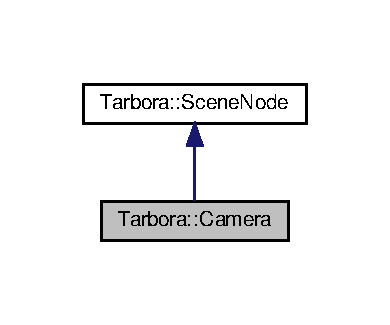
\includegraphics[width=187pt]{classTarbora_1_1Camera__inherit__graph}
\end{center}
\end{figure}


Collaboration diagram for Tarbora\+:\+:Camera\+:\nopagebreak
\begin{figure}[H]
\begin{center}
\leavevmode
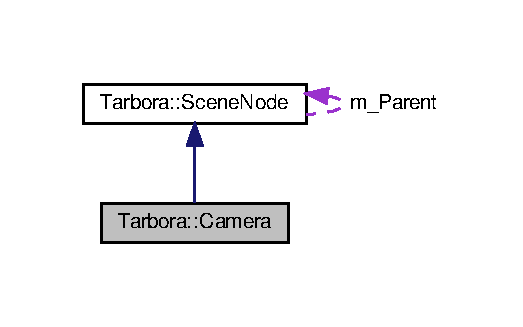
\includegraphics[width=251pt]{classTarbora_1_1Camera__coll__graph}
\end{center}
\end{figure}
\subsection*{Public Member Functions}
\begin{DoxyCompactItemize}
\item 
\mbox{\Hypertarget{classTarbora_1_1Camera_a45153edee036e9ffd270fe4ac4a5067d}\label{classTarbora_1_1Camera_a45153edee036e9ffd270fe4ac4a5067d}} 
{\bfseries Camera} (Actor\+Id actor\+Id, std\+::string name)
\item 
\mbox{\Hypertarget{classTarbora_1_1Camera_a0b29c84c5ac0c00e847c6690bda0ca3a}\label{classTarbora_1_1Camera_a0b29c84c5ac0c00e847c6690bda0ca3a}} 
const glm\+::mat4 {\bfseries Get\+View} ()
\item 
\mbox{\Hypertarget{classTarbora_1_1Camera_a57738b366d754a3657a865b75c23d8fc}\label{classTarbora_1_1Camera_a57738b366d754a3657a865b75c23d8fc}} 
const glm\+::mat4 {\bfseries Get\+View\+Angle} ()
\end{DoxyCompactItemize}
\subsection*{Additional Inherited Members}


The documentation for this class was generated from the following files\+:\begin{DoxyCompactItemize}
\item 
Tarbora/\+Views/\+Graphic\+Views/inc/Scene\+Node.\+hpp\item 
Tarbora/\+Views/\+Graphic\+Views/src/Scene\+Node.\+cpp\end{DoxyCompactItemize}

\hypertarget{classTarbora_1_1CapsuleBody}{}\section{Tarbora\+:\+:Capsule\+Body Class Reference}
\label{classTarbora_1_1CapsuleBody}\index{Tarbora\+::\+Capsule\+Body@{Tarbora\+::\+Capsule\+Body}}


A physics rigid body representing an capsule shape.  




{\ttfamily \#include $<$Rigid\+Body.\+hpp$>$}



Inheritance diagram for Tarbora\+:\+:Capsule\+Body\+:\nopagebreak
\begin{figure}[H]
\begin{center}
\leavevmode
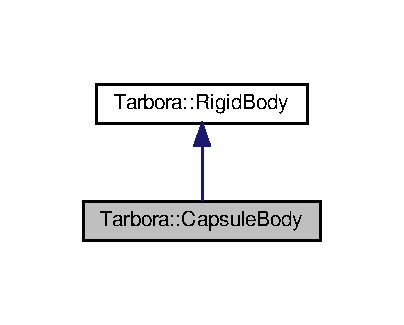
\includegraphics[width=194pt]{classTarbora_1_1CapsuleBody__inherit__graph}
\end{center}
\end{figure}


Collaboration diagram for Tarbora\+:\+:Capsule\+Body\+:\nopagebreak
\begin{figure}[H]
\begin{center}
\leavevmode
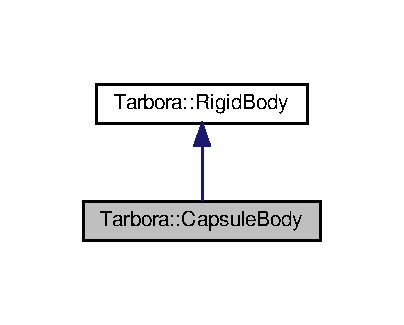
\includegraphics[width=194pt]{classTarbora_1_1CapsuleBody__coll__graph}
\end{center}
\end{figure}
\subsection*{Public Member Functions}
\begin{DoxyCompactItemize}
\item 
\hyperlink{classTarbora_1_1CapsuleBody_ac7427a8fd201d1eb99944d48619e78ed}{Capsule\+Body} (float radius, float height)
\begin{DoxyCompactList}\small\item\em Creates an \hyperlink{classTarbora_1_1CapsuleBody}{Capsule\+Body}. \end{DoxyCompactList}\item 
\mbox{\Hypertarget{classTarbora_1_1CapsuleBody_a70eeff3b16e27269076fef05a42a7de8}\label{classTarbora_1_1CapsuleBody_a70eeff3b16e27269076fef05a42a7de8}} 
\hyperlink{classTarbora_1_1CapsuleBody_a70eeff3b16e27269076fef05a42a7de8}{$\sim$\+Capsule\+Body} ()
\begin{DoxyCompactList}\small\item\em Destroys and unregisters this body. \end{DoxyCompactList}\item 
virtual void \hyperlink{classTarbora_1_1CapsuleBody_a4613a4f0cf0ab92189169d6f3865274e}{register\+Actor} (Actor\+Id \&id, const glm\+::vec3 \&position, const glm\+::quat \&rotation) override
\begin{DoxyCompactList}\small\item\em Register the rigid body to the Physics Engine. \end{DoxyCompactList}\item 
\mbox{\Hypertarget{classTarbora_1_1CapsuleBody_a3cce96469ed469136728ed0ea3004bc0}\label{classTarbora_1_1CapsuleBody_a3cce96469ed469136728ed0ea3004bc0}} 
virtual void \hyperlink{classTarbora_1_1CapsuleBody_a3cce96469ed469136728ed0ea3004bc0}{unregister} () override
\begin{DoxyCompactList}\small\item\em Remove the rigid body from the Physics Engine. \end{DoxyCompactList}\item 
\mbox{\Hypertarget{classTarbora_1_1CapsuleBody_a16af8c987d2a1d6602a317850b0ae17a}\label{classTarbora_1_1CapsuleBody_a16af8c987d2a1d6602a317850b0ae17a}} 
virtual void \hyperlink{classTarbora_1_1CapsuleBody_a16af8c987d2a1d6602a317850b0ae17a}{calc\+Volume} () override
\begin{DoxyCompactList}\small\item\em Calculate the volume when the shape or the size changes. Automatically called by the functions that change those. \end{DoxyCompactList}\item 
void \hyperlink{classTarbora_1_1CapsuleBody_a10ae8b263f437a7d810f727cd7e7e943}{set\+Radius} (float radius)
\begin{DoxyCompactList}\small\item\em Set the radius of that capsule. \end{DoxyCompactList}\item 
\mbox{\Hypertarget{classTarbora_1_1CapsuleBody_a3c4217bfdf918f48a49221e07aee262c}\label{classTarbora_1_1CapsuleBody_a3c4217bfdf918f48a49221e07aee262c}} 
float \hyperlink{classTarbora_1_1CapsuleBody_a3c4217bfdf918f48a49221e07aee262c}{get\+Radius} ()
\begin{DoxyCompactList}\small\item\em Get the radius of that sphere. \end{DoxyCompactList}\item 
void \hyperlink{classTarbora_1_1CapsuleBody_a8ecfb8196d5156649b8e04256e1d63c1}{set\+Height} (float height)
\begin{DoxyCompactList}\small\item\em Set the height of that capsule. \end{DoxyCompactList}\item 
\mbox{\Hypertarget{classTarbora_1_1CapsuleBody_a521b8b538755f1f72c7298a4a291053d}\label{classTarbora_1_1CapsuleBody_a521b8b538755f1f72c7298a4a291053d}} 
float \hyperlink{classTarbora_1_1CapsuleBody_a521b8b538755f1f72c7298a4a291053d}{get\+Height} ()
\begin{DoxyCompactList}\small\item\em Get the height of that sphere. \end{DoxyCompactList}\end{DoxyCompactItemize}
\subsection*{Additional Inherited Members}


\subsection{Detailed Description}
A physics rigid body representing an capsule shape. 

\begin{DoxySeeAlso}{See also}
\hyperlink{classTarbora_1_1PhysicsEngine}{Physics\+Engine} 

\hyperlink{classTarbora_1_1RigidBody}{Rigid\+Body} 

\hyperlink{classTarbora_1_1SphereBody}{Sphere\+Body} 
\end{DoxySeeAlso}


\subsection{Constructor \& Destructor Documentation}
\mbox{\Hypertarget{classTarbora_1_1CapsuleBody_ac7427a8fd201d1eb99944d48619e78ed}\label{classTarbora_1_1CapsuleBody_ac7427a8fd201d1eb99944d48619e78ed}} 
\index{Tarbora\+::\+Capsule\+Body@{Tarbora\+::\+Capsule\+Body}!Capsule\+Body@{Capsule\+Body}}
\index{Capsule\+Body@{Capsule\+Body}!Tarbora\+::\+Capsule\+Body@{Tarbora\+::\+Capsule\+Body}}
\subsubsection{\texorpdfstring{Capsule\+Body()}{CapsuleBody()}}
{\footnotesize\ttfamily Tarbora\+::\+Capsule\+Body\+::\+Capsule\+Body (\begin{DoxyParamCaption}\item[{float}]{radius,  }\item[{float}]{height }\end{DoxyParamCaption})}



Creates an \hyperlink{classTarbora_1_1CapsuleBody}{Capsule\+Body}. 


\begin{DoxyParams}{Parameters}
{\em radius} & The radius of that capsule, used to calculate the volume and the mass. \\
\hline
{\em height} & The height of that capsule, used to calculate the volume and the mass. \\
\hline
\end{DoxyParams}


\subsection{Member Function Documentation}
\mbox{\Hypertarget{classTarbora_1_1CapsuleBody_a4613a4f0cf0ab92189169d6f3865274e}\label{classTarbora_1_1CapsuleBody_a4613a4f0cf0ab92189169d6f3865274e}} 
\index{Tarbora\+::\+Capsule\+Body@{Tarbora\+::\+Capsule\+Body}!register\+Actor@{register\+Actor}}
\index{register\+Actor@{register\+Actor}!Tarbora\+::\+Capsule\+Body@{Tarbora\+::\+Capsule\+Body}}
\subsubsection{\texorpdfstring{register\+Actor()}{registerActor()}}
{\footnotesize\ttfamily void Tarbora\+::\+Capsule\+Body\+::register\+Actor (\begin{DoxyParamCaption}\item[{Actor\+Id \&}]{id,  }\item[{const glm\+::vec3 \&}]{position,  }\item[{const glm\+::quat \&}]{rotation }\end{DoxyParamCaption})\hspace{0.3cm}{\ttfamily [override]}, {\ttfamily [virtual]}}



Register the rigid body to the Physics Engine. 


\begin{DoxyParams}{Parameters}
{\em id} & The id of the actor that owns that rigid body. \\
\hline
{\em position} & The initial position of that actor. \\
\hline
{\em rotation} & The initial rotation of that actor. \\
\hline
\end{DoxyParams}


Implements \hyperlink{classTarbora_1_1RigidBody_acd1c63e93fd607f74f48fb68aa764b29}{Tarbora\+::\+Rigid\+Body}.

\mbox{\Hypertarget{classTarbora_1_1CapsuleBody_a8ecfb8196d5156649b8e04256e1d63c1}\label{classTarbora_1_1CapsuleBody_a8ecfb8196d5156649b8e04256e1d63c1}} 
\index{Tarbora\+::\+Capsule\+Body@{Tarbora\+::\+Capsule\+Body}!set\+Height@{set\+Height}}
\index{set\+Height@{set\+Height}!Tarbora\+::\+Capsule\+Body@{Tarbora\+::\+Capsule\+Body}}
\subsubsection{\texorpdfstring{set\+Height()}{setHeight()}}
{\footnotesize\ttfamily void Tarbora\+::\+Capsule\+Body\+::set\+Height (\begin{DoxyParamCaption}\item[{float}]{height }\end{DoxyParamCaption})\hspace{0.3cm}{\ttfamily [inline]}}



Set the height of that capsule. 


\begin{DoxyParams}{Parameters}
{\em height} & The height of that capsule, used to calculate the volume and the mass. \\
\hline
\end{DoxyParams}
\mbox{\Hypertarget{classTarbora_1_1CapsuleBody_a10ae8b263f437a7d810f727cd7e7e943}\label{classTarbora_1_1CapsuleBody_a10ae8b263f437a7d810f727cd7e7e943}} 
\index{Tarbora\+::\+Capsule\+Body@{Tarbora\+::\+Capsule\+Body}!set\+Radius@{set\+Radius}}
\index{set\+Radius@{set\+Radius}!Tarbora\+::\+Capsule\+Body@{Tarbora\+::\+Capsule\+Body}}
\subsubsection{\texorpdfstring{set\+Radius()}{setRadius()}}
{\footnotesize\ttfamily void Tarbora\+::\+Capsule\+Body\+::set\+Radius (\begin{DoxyParamCaption}\item[{float}]{radius }\end{DoxyParamCaption})\hspace{0.3cm}{\ttfamily [inline]}}



Set the radius of that capsule. 


\begin{DoxyParams}{Parameters}
{\em radius} & The radius of that capsule, used to calculate the volume and the mass. \\
\hline
\end{DoxyParams}


The documentation for this class was generated from the following files\+:\begin{DoxyCompactItemize}
\item 
Tarbora/\+Logic/\+Physics\+Engine/Rigid\+Body.\+hpp\item 
Tarbora/\+Logic/\+Physics\+Engine/Rigid\+Body.\+cpp\end{DoxyCompactItemize}

\hypertarget{classTarbora_1_1CharacterControllerComponent}{}\section{Tarbora\+:\+:Character\+Controller\+Component Class Reference}
\label{classTarbora_1_1CharacterControllerComponent}\index{Tarbora\+::\+Character\+Controller\+Component@{Tarbora\+::\+Character\+Controller\+Component}}


Inheritance diagram for Tarbora\+:\+:Character\+Controller\+Component\+:
\nopagebreak
\begin{figure}[H]
\begin{center}
\leavevmode
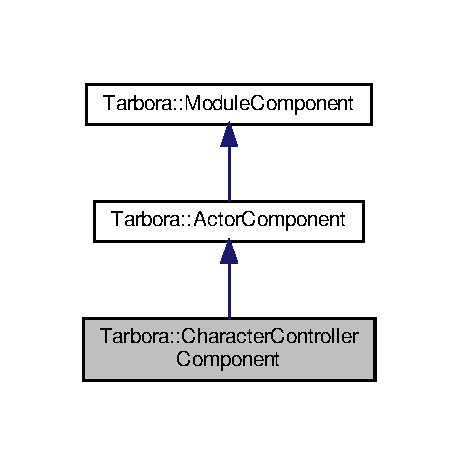
\includegraphics[width=220pt]{classTarbora_1_1CharacterControllerComponent__inherit__graph}
\end{center}
\end{figure}


Collaboration diagram for Tarbora\+:\+:Character\+Controller\+Component\+:
\nopagebreak
\begin{figure}[H]
\begin{center}
\leavevmode
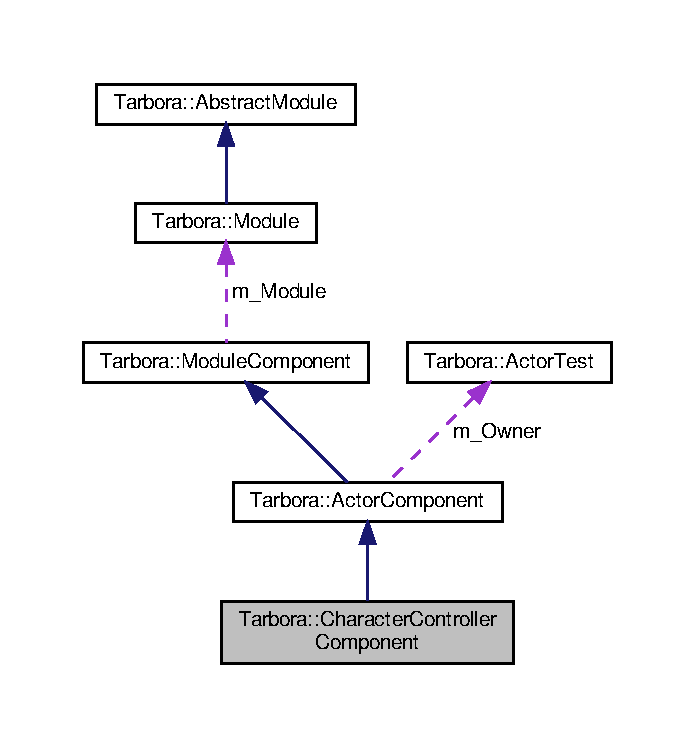
\includegraphics[width=334pt]{classTarbora_1_1CharacterControllerComponent__coll__graph}
\end{center}
\end{figure}
\subsection*{Public Member Functions}
\begin{DoxyCompactItemize}
\item 
\mbox{\Hypertarget{classTarbora_1_1CharacterControllerComponent_a2973a925ac0459deaa9fd7d390c66e3f}\label{classTarbora_1_1CharacterControllerComponent_a2973a925ac0459deaa9fd7d390c66e3f}} 
{\bfseries Character\+Controller\+Component} (\hyperlink{classTarbora_1_1World}{World} $\ast$world)
\item 
\mbox{\Hypertarget{classTarbora_1_1CharacterControllerComponent_a5929fff77727c8bee445736b6a4c69d8}\label{classTarbora_1_1CharacterControllerComponent_a5929fff77727c8bee445736b6a4c69d8}} 
Component\+Id {\bfseries Get\+Id} () const
\item 
\mbox{\Hypertarget{classTarbora_1_1CharacterControllerComponent_aa70e4199ad42f87528ef0366d3b62b53}\label{classTarbora_1_1CharacterControllerComponent_aa70e4199ad42f87528ef0366d3b62b53}} 
bool {\bfseries Init} (Json\+Ptr resource, raw\+\_\+json data)
\item 
\mbox{\Hypertarget{classTarbora_1_1CharacterControllerComponent_a3e909ef055662f0f898f19cc5212482c}\label{classTarbora_1_1CharacterControllerComponent_a3e909ef055662f0f898f19cc5212482c}} 
void {\bfseries After\+Init} ()
\item 
\mbox{\Hypertarget{classTarbora_1_1CharacterControllerComponent_a302d5f23db1b6b1053ed9c5c2b24f093}\label{classTarbora_1_1CharacterControllerComponent_a302d5f23db1b6b1053ed9c5c2b24f093}} 
virtual void {\bfseries Update} (float delta\+Time) override
\end{DoxyCompactItemize}
\subsection*{Static Public Member Functions}
\begin{DoxyCompactItemize}
\item 
\mbox{\Hypertarget{classTarbora_1_1CharacterControllerComponent_a01fd385c667b068703620d6a3e59fdf9}\label{classTarbora_1_1CharacterControllerComponent_a01fd385c667b068703620d6a3e59fdf9}} 
static Actor\+Component\+Ptr {\bfseries Creator} (\hyperlink{classTarbora_1_1World}{World} $\ast$world)
\end{DoxyCompactItemize}
\subsection*{Additional Inherited Members}


The documentation for this class was generated from the following files\+:\begin{DoxyCompactItemize}
\item 
Tarbora/\+Logic/inc/Character\+Controller\+Component.\+hpp\item 
Tarbora/\+Logic/src/Character\+Controller\+Component.\+cpp\end{DoxyCompactItemize}

\hypertarget{classTarbora_1_1ConsoleImpl}{}\section{Tarbora\+:\+:Console\+Impl Class Reference}
\label{classTarbora_1_1ConsoleImpl}\index{Tarbora\+::\+Console\+Impl@{Tarbora\+::\+Console\+Impl}}


Inheritance diagram for Tarbora\+:\+:Console\+Impl\+:
\nopagebreak
\begin{figure}[H]
\begin{center}
\leavevmode
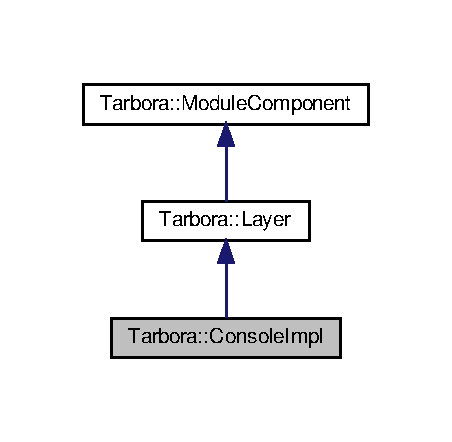
\includegraphics[width=217pt]{classTarbora_1_1ConsoleImpl__inherit__graph}
\end{center}
\end{figure}


Collaboration diagram for Tarbora\+:\+:Console\+Impl\+:
\nopagebreak
\begin{figure}[H]
\begin{center}
\leavevmode
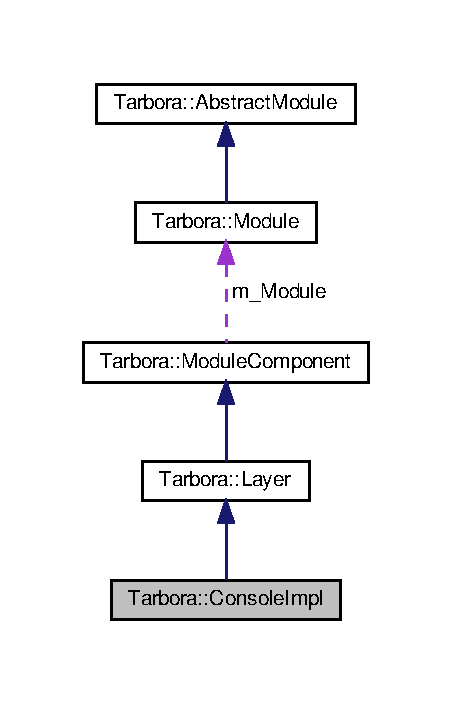
\includegraphics[width=217pt]{classTarbora_1_1ConsoleImpl__coll__graph}
\end{center}
\end{figure}
\subsection*{Public Member Functions}
\begin{DoxyCompactItemize}
\item 
\mbox{\Hypertarget{classTarbora_1_1ConsoleImpl_aff56ef0e6e2e284636cb9b5f2809448d}\label{classTarbora_1_1ConsoleImpl_aff56ef0e6e2e284636cb9b5f2809448d}} 
{\bfseries Console\+Impl} (\hyperlink{classTarbora_1_1GraphicView}{Graphic\+View} $\ast$view, bool start\+\_\+active, bool full\+Window, Input\+Callback callback)
\item 
\mbox{\Hypertarget{classTarbora_1_1ConsoleImpl_a772dedbf29837c81cd8a4799bbad6ae2}\label{classTarbora_1_1ConsoleImpl_a772dedbf29837c81cd8a4799bbad6ae2}} 
void {\bfseries Get\+Input} () override
\item 
\mbox{\Hypertarget{classTarbora_1_1ConsoleImpl_adfb33b8aa112331409e84c1f87fb2cd9}\label{classTarbora_1_1ConsoleImpl_adfb33b8aa112331409e84c1f87fb2cd9}} 
void {\bfseries Log} (std\+::string text)
\item 
\mbox{\Hypertarget{classTarbora_1_1ConsoleImpl_ad9c1f99c73b1bb80fa384b9db26b33fb}\label{classTarbora_1_1ConsoleImpl_ad9c1f99c73b1bb80fa384b9db26b33fb}} 
void {\bfseries Draw} () override
\end{DoxyCompactItemize}
\subsection*{Additional Inherited Members}


The documentation for this class was generated from the following file\+:\begin{DoxyCompactItemize}
\item 
Tarbora/\+Views/\+Graphic\+Views/inc/Console.\+hpp\end{DoxyCompactItemize}

\hypertarget{classTarbora_1_1CreateActor}{}\section{Tarbora\+:\+:Create\+Actor Class Reference}
\label{classTarbora_1_1CreateActor}\index{Tarbora\+::\+Create\+Actor@{Tarbora\+::\+Create\+Actor}}


Inheritance diagram for Tarbora\+:\+:Create\+Actor\+:
\nopagebreak
\begin{figure}[H]
\begin{center}
\leavevmode
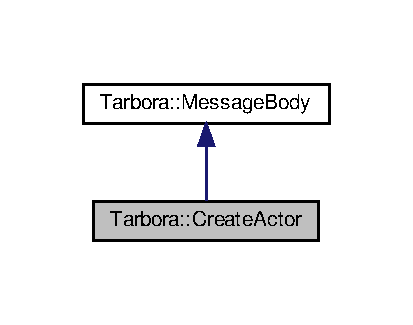
\includegraphics[width=198pt]{classTarbora_1_1CreateActor__inherit__graph}
\end{center}
\end{figure}


Collaboration diagram for Tarbora\+:\+:Create\+Actor\+:
\nopagebreak
\begin{figure}[H]
\begin{center}
\leavevmode
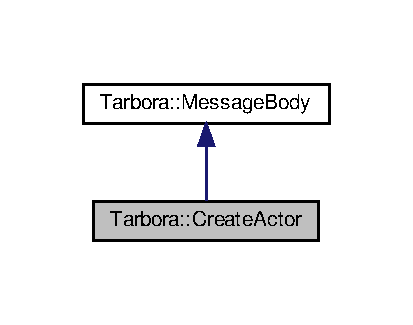
\includegraphics[width=198pt]{classTarbora_1_1CreateActor__coll__graph}
\end{center}
\end{figure}
\subsection*{Public Member Functions}
\begin{DoxyCompactItemize}
\item 
\mbox{\Hypertarget{classTarbora_1_1CreateActor_a8bd921da8eeba3df7cce996eb1baf271}\label{classTarbora_1_1CreateActor_a8bd921da8eeba3df7cce996eb1baf271}} 
{\bfseries Create\+Actor} (unsigned int id, std\+::string entity, std\+::string variant, glm\+::vec3 position=glm\+::vec3(), glm\+::vec3 rotation=glm\+::vec3())
\end{DoxyCompactItemize}
\subsection*{Additional Inherited Members}


The documentation for this class was generated from the following file\+:\begin{DoxyCompactItemize}
\item 
Tarbora/\+Messages/Basic\+Messages.\+hpp\end{DoxyCompactItemize}

\hypertarget{classtbBasics_1_1CreateActorBody}{}\section{tb\+Basics\+:\+:Create\+Actor\+Body Class Reference}
\label{classtbBasics_1_1CreateActorBody}\index{tb\+Basics\+::\+Create\+Actor\+Body@{tb\+Basics\+::\+Create\+Actor\+Body}}


Inheritance diagram for tb\+Basics\+:\+:Create\+Actor\+Body\+:
\nopagebreak
\begin{figure}[H]
\begin{center}
\leavevmode
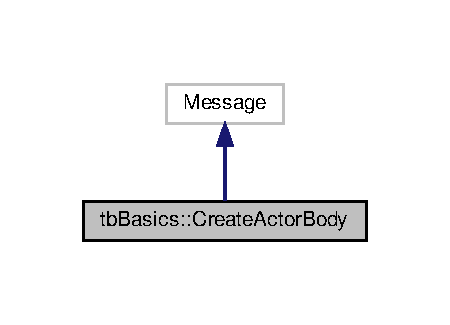
\includegraphics[width=216pt]{classtbBasics_1_1CreateActorBody__inherit__graph}
\end{center}
\end{figure}


Collaboration diagram for tb\+Basics\+:\+:Create\+Actor\+Body\+:
\nopagebreak
\begin{figure}[H]
\begin{center}
\leavevmode
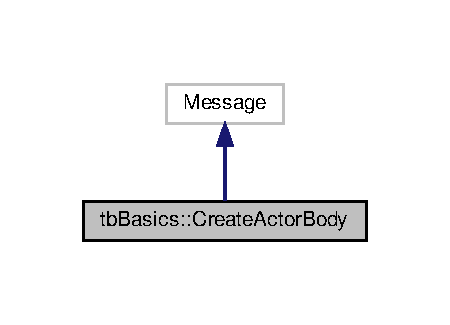
\includegraphics[width=216pt]{classtbBasics_1_1CreateActorBody__coll__graph}
\end{center}
\end{figure}
\subsection*{Classes}
\begin{DoxyCompactItemize}
\item 
class \hyperlink{classtbBasics_1_1CreateActorBody_1_1HasBitSetters}{Has\+Bit\+Setters}
\end{DoxyCompactItemize}
\subsection*{Public Member Functions}
\begin{DoxyCompactItemize}
\item 
\mbox{\Hypertarget{classtbBasics_1_1CreateActorBody_a4227ff7ff1f60f792a3b97a793dc2862}\label{classtbBasics_1_1CreateActorBody_a4227ff7ff1f60f792a3b97a793dc2862}} 
{\bfseries Create\+Actor\+Body} (const \hyperlink{classtbBasics_1_1CreateActorBody}{Create\+Actor\+Body} \&from)
\item 
\mbox{\Hypertarget{classtbBasics_1_1CreateActorBody_a0622d7bfb7da8c3efd2eaab74aeaf511}\label{classtbBasics_1_1CreateActorBody_a0622d7bfb7da8c3efd2eaab74aeaf511}} 
\hyperlink{classtbBasics_1_1CreateActorBody}{Create\+Actor\+Body} \& {\bfseries operator=} (const \hyperlink{classtbBasics_1_1CreateActorBody}{Create\+Actor\+Body} \&from)
\item 
\mbox{\Hypertarget{classtbBasics_1_1CreateActorBody_afd40d70bcc48ca08c552a4e7a4c0c8c6}\label{classtbBasics_1_1CreateActorBody_afd40d70bcc48ca08c552a4e7a4c0c8c6}} 
void {\bfseries Swap} (\hyperlink{classtbBasics_1_1CreateActorBody}{Create\+Actor\+Body} $\ast$other)
\item 
\mbox{\Hypertarget{classtbBasics_1_1CreateActorBody_ac27f1379b5e5cf1f4d48bba69747ef07}\label{classtbBasics_1_1CreateActorBody_ac27f1379b5e5cf1f4d48bba69747ef07}} 
\hyperlink{classtbBasics_1_1CreateActorBody}{Create\+Actor\+Body} $\ast$ {\bfseries New} () const final
\item 
\mbox{\Hypertarget{classtbBasics_1_1CreateActorBody_a03daca41ae34ae0c2802837d751b701e}\label{classtbBasics_1_1CreateActorBody_a03daca41ae34ae0c2802837d751b701e}} 
\hyperlink{classtbBasics_1_1CreateActorBody}{Create\+Actor\+Body} $\ast$ {\bfseries New} (\+::google\+::protobuf\+::\+Arena $\ast$arena) const final
\item 
\mbox{\Hypertarget{classtbBasics_1_1CreateActorBody_a6d5b173a1a28c7e2ed1a995d4bf0b687}\label{classtbBasics_1_1CreateActorBody_a6d5b173a1a28c7e2ed1a995d4bf0b687}} 
void {\bfseries Copy\+From} (const \+::google\+::protobuf\+::\+Message \&from) final
\item 
\mbox{\Hypertarget{classtbBasics_1_1CreateActorBody_a7ea37b3f9cec2883a468859907da8181}\label{classtbBasics_1_1CreateActorBody_a7ea37b3f9cec2883a468859907da8181}} 
void {\bfseries Merge\+From} (const \+::google\+::protobuf\+::\+Message \&from) final
\item 
\mbox{\Hypertarget{classtbBasics_1_1CreateActorBody_a1b9ec0c3b0815e6d56472ba830910d71}\label{classtbBasics_1_1CreateActorBody_a1b9ec0c3b0815e6d56472ba830910d71}} 
void {\bfseries Copy\+From} (const \hyperlink{classtbBasics_1_1CreateActorBody}{Create\+Actor\+Body} \&from)
\item 
\mbox{\Hypertarget{classtbBasics_1_1CreateActorBody_a893e4164a9749ab481e5f463f6695b91}\label{classtbBasics_1_1CreateActorBody_a893e4164a9749ab481e5f463f6695b91}} 
void {\bfseries Merge\+From} (const \hyperlink{classtbBasics_1_1CreateActorBody}{Create\+Actor\+Body} \&from)
\item 
\mbox{\Hypertarget{classtbBasics_1_1CreateActorBody_a454713a2ad9dd185c6998bdd20b80c14}\label{classtbBasics_1_1CreateActorBody_a454713a2ad9dd185c6998bdd20b80c14}} 
P\+R\+O\+T\+O\+B\+U\+F\+\_\+\+A\+T\+T\+R\+I\+B\+U\+T\+E\+\_\+\+R\+E\+I\+N\+I\+T\+I\+A\+L\+I\+Z\+ES void {\bfseries Clear} () final
\item 
\mbox{\Hypertarget{classtbBasics_1_1CreateActorBody_ada053422e783353b081e32922bd596e1}\label{classtbBasics_1_1CreateActorBody_ada053422e783353b081e32922bd596e1}} 
bool {\bfseries Is\+Initialized} () const final
\item 
\mbox{\Hypertarget{classtbBasics_1_1CreateActorBody_afffd08653ca7275be758f9c21efa78b3}\label{classtbBasics_1_1CreateActorBody_afffd08653ca7275be758f9c21efa78b3}} 
size\+\_\+t {\bfseries Byte\+Size\+Long} () const final
\item 
\mbox{\Hypertarget{classtbBasics_1_1CreateActorBody_a58275a21c782e394b9a6e72c27890e93}\label{classtbBasics_1_1CreateActorBody_a58275a21c782e394b9a6e72c27890e93}} 
bool {\bfseries Merge\+Partial\+From\+Coded\+Stream} (\+::google\+::protobuf\+::io\+::\+Coded\+Input\+Stream $\ast$input) final
\item 
\mbox{\Hypertarget{classtbBasics_1_1CreateActorBody_a4786109ab6492d6136cc01f2930a58b9}\label{classtbBasics_1_1CreateActorBody_a4786109ab6492d6136cc01f2930a58b9}} 
void {\bfseries Serialize\+With\+Cached\+Sizes} (\+::google\+::protobuf\+::io\+::\+Coded\+Output\+Stream $\ast$output) const final
\item 
\mbox{\Hypertarget{classtbBasics_1_1CreateActorBody_af95810c32088b0cf88a871726d992482}\label{classtbBasics_1_1CreateActorBody_af95810c32088b0cf88a871726d992482}} 
\+::google\+::protobuf\+::uint8 $\ast$ {\bfseries Internal\+Serialize\+With\+Cached\+Sizes\+To\+Array} (\+::google\+::protobuf\+::uint8 $\ast$target) const final
\item 
\mbox{\Hypertarget{classtbBasics_1_1CreateActorBody_a13687241e582a665c14e0d164bced45e}\label{classtbBasics_1_1CreateActorBody_a13687241e582a665c14e0d164bced45e}} 
int {\bfseries Get\+Cached\+Size} () const final
\item 
\mbox{\Hypertarget{classtbBasics_1_1CreateActorBody_a5c3886a60e9ef32e567041d0c87b724b}\label{classtbBasics_1_1CreateActorBody_a5c3886a60e9ef32e567041d0c87b724b}} 
\+::google\+::protobuf\+::\+Metadata {\bfseries Get\+Metadata} () const final
\item 
\mbox{\Hypertarget{classtbBasics_1_1CreateActorBody_a4f68883162cf9739de7dacc3c75b6595}\label{classtbBasics_1_1CreateActorBody_a4f68883162cf9739de7dacc3c75b6595}} 
void {\bfseries clear\+\_\+entity} ()
\item 
\mbox{\Hypertarget{classtbBasics_1_1CreateActorBody_a7289a9ea60b3ddac9e0e5680957132b8}\label{classtbBasics_1_1CreateActorBody_a7289a9ea60b3ddac9e0e5680957132b8}} 
const \+::std\+::string \& {\bfseries entity} () const
\item 
\mbox{\Hypertarget{classtbBasics_1_1CreateActorBody_a291e39e542fa1beca0ed16eec4234ce6}\label{classtbBasics_1_1CreateActorBody_a291e39e542fa1beca0ed16eec4234ce6}} 
void {\bfseries set\+\_\+entity} (const \+::std\+::string \&value)
\item 
\mbox{\Hypertarget{classtbBasics_1_1CreateActorBody_abeb0dd8815ad4feba11d6d7c8f647ae2}\label{classtbBasics_1_1CreateActorBody_abeb0dd8815ad4feba11d6d7c8f647ae2}} 
void {\bfseries set\+\_\+entity} (const char $\ast$value)
\item 
\mbox{\Hypertarget{classtbBasics_1_1CreateActorBody_a87e16f806354c9880ad15ea00e16836f}\label{classtbBasics_1_1CreateActorBody_a87e16f806354c9880ad15ea00e16836f}} 
void {\bfseries set\+\_\+entity} (const char $\ast$value, size\+\_\+t size)
\item 
\mbox{\Hypertarget{classtbBasics_1_1CreateActorBody_aa1f8a1714d6cfe78c4d29e644fb61d08}\label{classtbBasics_1_1CreateActorBody_aa1f8a1714d6cfe78c4d29e644fb61d08}} 
\+::std\+::string $\ast$ {\bfseries mutable\+\_\+entity} ()
\item 
\mbox{\Hypertarget{classtbBasics_1_1CreateActorBody_ac2601e08a78e247974d8998969a37c3d}\label{classtbBasics_1_1CreateActorBody_ac2601e08a78e247974d8998969a37c3d}} 
\+::std\+::string $\ast$ {\bfseries release\+\_\+entity} ()
\item 
\mbox{\Hypertarget{classtbBasics_1_1CreateActorBody_a543a019bd607ca9562ef5c32fe3fe5a2}\label{classtbBasics_1_1CreateActorBody_a543a019bd607ca9562ef5c32fe3fe5a2}} 
void {\bfseries set\+\_\+allocated\+\_\+entity} (\+::std\+::string $\ast$entity)
\item 
\mbox{\Hypertarget{classtbBasics_1_1CreateActorBody_a3234dba226faaee530a827531b12481b}\label{classtbBasics_1_1CreateActorBody_a3234dba226faaee530a827531b12481b}} 
void {\bfseries clear\+\_\+variant} ()
\item 
\mbox{\Hypertarget{classtbBasics_1_1CreateActorBody_abc73a2d0bf8262be9235bee7e35ce695}\label{classtbBasics_1_1CreateActorBody_abc73a2d0bf8262be9235bee7e35ce695}} 
const \+::std\+::string \& {\bfseries variant} () const
\item 
\mbox{\Hypertarget{classtbBasics_1_1CreateActorBody_a43824f81b4630285dd5f180057424041}\label{classtbBasics_1_1CreateActorBody_a43824f81b4630285dd5f180057424041}} 
void {\bfseries set\+\_\+variant} (const \+::std\+::string \&value)
\item 
\mbox{\Hypertarget{classtbBasics_1_1CreateActorBody_a89c89f37663aa2eb367457f74e0ba1a7}\label{classtbBasics_1_1CreateActorBody_a89c89f37663aa2eb367457f74e0ba1a7}} 
void {\bfseries set\+\_\+variant} (const char $\ast$value)
\item 
\mbox{\Hypertarget{classtbBasics_1_1CreateActorBody_a217038f6e8a4a40a7fae1e1c5ee77328}\label{classtbBasics_1_1CreateActorBody_a217038f6e8a4a40a7fae1e1c5ee77328}} 
void {\bfseries set\+\_\+variant} (const char $\ast$value, size\+\_\+t size)
\item 
\mbox{\Hypertarget{classtbBasics_1_1CreateActorBody_ad93243b9da9fd59c40e351d49b2cc535}\label{classtbBasics_1_1CreateActorBody_ad93243b9da9fd59c40e351d49b2cc535}} 
\+::std\+::string $\ast$ {\bfseries mutable\+\_\+variant} ()
\item 
\mbox{\Hypertarget{classtbBasics_1_1CreateActorBody_a162ccedd90c8ce5d4b2439a253413d03}\label{classtbBasics_1_1CreateActorBody_a162ccedd90c8ce5d4b2439a253413d03}} 
\+::std\+::string $\ast$ {\bfseries release\+\_\+variant} ()
\item 
\mbox{\Hypertarget{classtbBasics_1_1CreateActorBody_a6808f59c948fc0e15c418dcfbecbd9db}\label{classtbBasics_1_1CreateActorBody_a6808f59c948fc0e15c418dcfbecbd9db}} 
void {\bfseries set\+\_\+allocated\+\_\+variant} (\+::std\+::string $\ast$variant)
\item 
\mbox{\Hypertarget{classtbBasics_1_1CreateActorBody_a0d616ccc18a6ca1c0ee76762918da9c2}\label{classtbBasics_1_1CreateActorBody_a0d616ccc18a6ca1c0ee76762918da9c2}} 
bool {\bfseries has\+\_\+position} () const
\item 
\mbox{\Hypertarget{classtbBasics_1_1CreateActorBody_a30bba5253579416a3e235357496b568d}\label{classtbBasics_1_1CreateActorBody_a30bba5253579416a3e235357496b568d}} 
void {\bfseries clear\+\_\+position} ()
\item 
\mbox{\Hypertarget{classtbBasics_1_1CreateActorBody_a42ca61eef78e7c347d0392a561b68aec}\label{classtbBasics_1_1CreateActorBody_a42ca61eef78e7c347d0392a561b68aec}} 
const \+::\hyperlink{classtbMath_1_1Vec3Message}{tb\+Math\+::\+Vec3\+Message} \& {\bfseries position} () const
\item 
\mbox{\Hypertarget{classtbBasics_1_1CreateActorBody_a382eb67755e7e1933839f16ef3cb7c7d}\label{classtbBasics_1_1CreateActorBody_a382eb67755e7e1933839f16ef3cb7c7d}} 
\+::\hyperlink{classtbMath_1_1Vec3Message}{tb\+Math\+::\+Vec3\+Message} $\ast$ {\bfseries release\+\_\+position} ()
\item 
\mbox{\Hypertarget{classtbBasics_1_1CreateActorBody_af6d03301d80982c5768dc5bf50ffb42c}\label{classtbBasics_1_1CreateActorBody_af6d03301d80982c5768dc5bf50ffb42c}} 
\+::\hyperlink{classtbMath_1_1Vec3Message}{tb\+Math\+::\+Vec3\+Message} $\ast$ {\bfseries mutable\+\_\+position} ()
\item 
\mbox{\Hypertarget{classtbBasics_1_1CreateActorBody_ab2da59e15e052d5780cef32236f490cc}\label{classtbBasics_1_1CreateActorBody_ab2da59e15e052d5780cef32236f490cc}} 
void {\bfseries set\+\_\+allocated\+\_\+position} (\+::\hyperlink{classtbMath_1_1Vec3Message}{tb\+Math\+::\+Vec3\+Message} $\ast$position)
\item 
\mbox{\Hypertarget{classtbBasics_1_1CreateActorBody_af641ca8adc9f36012ce959eb2fe5f0cb}\label{classtbBasics_1_1CreateActorBody_af641ca8adc9f36012ce959eb2fe5f0cb}} 
bool {\bfseries has\+\_\+rotation} () const
\item 
\mbox{\Hypertarget{classtbBasics_1_1CreateActorBody_a9f67821ce923e170162170b1b32a13c0}\label{classtbBasics_1_1CreateActorBody_a9f67821ce923e170162170b1b32a13c0}} 
void {\bfseries clear\+\_\+rotation} ()
\item 
\mbox{\Hypertarget{classtbBasics_1_1CreateActorBody_a79b340a92840745295e0594640f55adf}\label{classtbBasics_1_1CreateActorBody_a79b340a92840745295e0594640f55adf}} 
const \+::\hyperlink{classtbMath_1_1Vec3Message}{tb\+Math\+::\+Vec3\+Message} \& {\bfseries rotation} () const
\item 
\mbox{\Hypertarget{classtbBasics_1_1CreateActorBody_a242112203d60b47b8e4a15d4f53c780b}\label{classtbBasics_1_1CreateActorBody_a242112203d60b47b8e4a15d4f53c780b}} 
\+::\hyperlink{classtbMath_1_1Vec3Message}{tb\+Math\+::\+Vec3\+Message} $\ast$ {\bfseries release\+\_\+rotation} ()
\item 
\mbox{\Hypertarget{classtbBasics_1_1CreateActorBody_aaf91be63b5bfeb63626fe1eddaeae343}\label{classtbBasics_1_1CreateActorBody_aaf91be63b5bfeb63626fe1eddaeae343}} 
\+::\hyperlink{classtbMath_1_1Vec3Message}{tb\+Math\+::\+Vec3\+Message} $\ast$ {\bfseries mutable\+\_\+rotation} ()
\item 
\mbox{\Hypertarget{classtbBasics_1_1CreateActorBody_a67038cb5defb4f008be5273f526b0544}\label{classtbBasics_1_1CreateActorBody_a67038cb5defb4f008be5273f526b0544}} 
void {\bfseries set\+\_\+allocated\+\_\+rotation} (\+::\hyperlink{classtbMath_1_1Vec3Message}{tb\+Math\+::\+Vec3\+Message} $\ast$rotation)
\item 
\mbox{\Hypertarget{classtbBasics_1_1CreateActorBody_a4dc1c1bff6cfad646cc5722d5d42747a}\label{classtbBasics_1_1CreateActorBody_a4dc1c1bff6cfad646cc5722d5d42747a}} 
void {\bfseries clear\+\_\+id} ()
\item 
\mbox{\Hypertarget{classtbBasics_1_1CreateActorBody_a19b7cc338fb743e7838440ad1c753a3b}\label{classtbBasics_1_1CreateActorBody_a19b7cc338fb743e7838440ad1c753a3b}} 
\+::google\+::protobuf\+::uint32 {\bfseries id} () const
\item 
\mbox{\Hypertarget{classtbBasics_1_1CreateActorBody_aa0b707761b9d7864dfdc9ba6de6c86cd}\label{classtbBasics_1_1CreateActorBody_aa0b707761b9d7864dfdc9ba6de6c86cd}} 
void {\bfseries set\+\_\+id} (\+::google\+::protobuf\+::uint32 value)
\end{DoxyCompactItemize}
\subsection*{Static Public Member Functions}
\begin{DoxyCompactItemize}
\item 
\mbox{\Hypertarget{classtbBasics_1_1CreateActorBody_a81ae0391f4244c31da403e2a2e8b6c32}\label{classtbBasics_1_1CreateActorBody_a81ae0391f4244c31da403e2a2e8b6c32}} 
static const \+::google\+::protobuf\+::\+Descriptor $\ast$ {\bfseries descriptor} ()
\item 
\mbox{\Hypertarget{classtbBasics_1_1CreateActorBody_a9c8744867212ca3d126d1e48573cbdb6}\label{classtbBasics_1_1CreateActorBody_a9c8744867212ca3d126d1e48573cbdb6}} 
static const \hyperlink{classtbBasics_1_1CreateActorBody}{Create\+Actor\+Body} \& {\bfseries default\+\_\+instance} ()
\item 
\mbox{\Hypertarget{classtbBasics_1_1CreateActorBody_a435b501601da8f5227cbba141d727f77}\label{classtbBasics_1_1CreateActorBody_a435b501601da8f5227cbba141d727f77}} 
static void {\bfseries Init\+As\+Default\+Instance} ()
\item 
\mbox{\Hypertarget{classtbBasics_1_1CreateActorBody_ae0e50a5444e6f43239575fbbb5c3040d}\label{classtbBasics_1_1CreateActorBody_ae0e50a5444e6f43239575fbbb5c3040d}} 
static const \hyperlink{classtbBasics_1_1CreateActorBody}{Create\+Actor\+Body} $\ast$ {\bfseries internal\+\_\+default\+\_\+instance} ()
\end{DoxyCompactItemize}
\subsection*{Static Public Attributes}
\begin{DoxyCompactItemize}
\item 
static constexpr int {\bfseries k\+Index\+In\+File\+Messages}
\item 
\mbox{\Hypertarget{classtbBasics_1_1CreateActorBody_a29209fbcdeba105c318b4aaaef6868ab}\label{classtbBasics_1_1CreateActorBody_a29209fbcdeba105c318b4aaaef6868ab}} 
static const int {\bfseries k\+Entity\+Field\+Number} = 2
\item 
\mbox{\Hypertarget{classtbBasics_1_1CreateActorBody_a93c5b2b328fcecb7beb7db7a13309a66}\label{classtbBasics_1_1CreateActorBody_a93c5b2b328fcecb7beb7db7a13309a66}} 
static const int {\bfseries k\+Variant\+Field\+Number} = 3
\item 
\mbox{\Hypertarget{classtbBasics_1_1CreateActorBody_ab6d8e4b96c318bf56dea31337e395948}\label{classtbBasics_1_1CreateActorBody_ab6d8e4b96c318bf56dea31337e395948}} 
static const int {\bfseries k\+Position\+Field\+Number} = 4
\item 
\mbox{\Hypertarget{classtbBasics_1_1CreateActorBody_a2318605d16675db083d9209f2abb7d0a}\label{classtbBasics_1_1CreateActorBody_a2318605d16675db083d9209f2abb7d0a}} 
static const int {\bfseries k\+Rotation\+Field\+Number} = 5
\item 
\mbox{\Hypertarget{classtbBasics_1_1CreateActorBody_a87e64026c0c6ec2033363cf090505589}\label{classtbBasics_1_1CreateActorBody_a87e64026c0c6ec2033363cf090505589}} 
static const int {\bfseries k\+Id\+Field\+Number} = 1
\end{DoxyCompactItemize}
\subsection*{Friends}
\begin{DoxyCompactItemize}
\item 
\mbox{\Hypertarget{classtbBasics_1_1CreateActorBody_ae86a2f4c520666b65d606ccbe2122e61}\label{classtbBasics_1_1CreateActorBody_ae86a2f4c520666b65d606ccbe2122e61}} 
struct {\bfseries \+::\+Table\+Struct\+\_\+basic\+\_\+2eproto}
\item 
\mbox{\Hypertarget{classtbBasics_1_1CreateActorBody_ae26a9b33544b5d0a394cdf0d91afc17b}\label{classtbBasics_1_1CreateActorBody_ae26a9b33544b5d0a394cdf0d91afc17b}} 
void {\bfseries swap} (\hyperlink{classtbBasics_1_1CreateActorBody}{Create\+Actor\+Body} \&a, \hyperlink{classtbBasics_1_1CreateActorBody}{Create\+Actor\+Body} \&b)
\end{DoxyCompactItemize}


\subsection{Member Data Documentation}
\mbox{\Hypertarget{classtbBasics_1_1CreateActorBody_a5294f04c77723a8625ad7e148c3011dd}\label{classtbBasics_1_1CreateActorBody_a5294f04c77723a8625ad7e148c3011dd}} 
\index{tb\+Basics\+::\+Create\+Actor\+Body@{tb\+Basics\+::\+Create\+Actor\+Body}!k\+Index\+In\+File\+Messages@{k\+Index\+In\+File\+Messages}}
\index{k\+Index\+In\+File\+Messages@{k\+Index\+In\+File\+Messages}!tb\+Basics\+::\+Create\+Actor\+Body@{tb\+Basics\+::\+Create\+Actor\+Body}}
\subsubsection{\texorpdfstring{k\+Index\+In\+File\+Messages}{kIndexInFileMessages}}
{\footnotesize\ttfamily constexpr int tb\+Basics\+::\+Create\+Actor\+Body\+::k\+Index\+In\+File\+Messages\hspace{0.3cm}{\ttfamily [static]}}

{\bfseries Initial value\+:}
\begin{DoxyCode}
=
    0
\end{DoxyCode}


The documentation for this class was generated from the following files\+:\begin{DoxyCompactItemize}
\item 
Tarbora/\+Messages/proto/basic.\+pb.\+h\item 
Tarbora/\+Messages/proto/basic.\+pb.\+cc\end{DoxyCompactItemize}

\hypertarget{classtbBasics_1_1CreateActorBodyDefaultTypeInternal}{}\section{tb\+Basics\+:\+:Create\+Actor\+Body\+Default\+Type\+Internal Class Reference}
\label{classtbBasics_1_1CreateActorBodyDefaultTypeInternal}\index{tb\+Basics\+::\+Create\+Actor\+Body\+Default\+Type\+Internal@{tb\+Basics\+::\+Create\+Actor\+Body\+Default\+Type\+Internal}}
\subsection*{Public Attributes}
\begin{DoxyCompactItemize}
\item 
\mbox{\Hypertarget{classtbBasics_1_1CreateActorBodyDefaultTypeInternal_a2a20362d9a76eb2c3e5069e93ee24698}\label{classtbBasics_1_1CreateActorBodyDefaultTypeInternal_a2a20362d9a76eb2c3e5069e93ee24698}} 
\+::google\+::protobuf\+::internal\+::\+Explicitly\+Constructed$<$ \hyperlink{classtbBasics_1_1CreateActorBody}{Create\+Actor\+Body} $>$ {\bfseries \+\_\+instance}
\end{DoxyCompactItemize}


The documentation for this class was generated from the following file\+:\begin{DoxyCompactItemize}
\item 
Tarbora/\+Messages/proto/basic.\+pb.\+cc\end{DoxyCompactItemize}

\hypertarget{classTarbora_1_1DeleteActor}{}\section{Tarbora\+:\+:Delete\+Actor Class Reference}
\label{classTarbora_1_1DeleteActor}\index{Tarbora\+::\+Delete\+Actor@{Tarbora\+::\+Delete\+Actor}}


Inheritance diagram for Tarbora\+:\+:Delete\+Actor\+:
\nopagebreak
\begin{figure}[H]
\begin{center}
\leavevmode
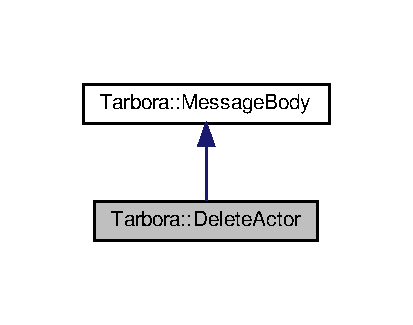
\includegraphics[width=198pt]{classTarbora_1_1DeleteActor__inherit__graph}
\end{center}
\end{figure}


Collaboration diagram for Tarbora\+:\+:Delete\+Actor\+:
\nopagebreak
\begin{figure}[H]
\begin{center}
\leavevmode
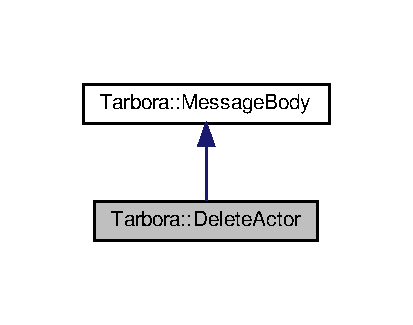
\includegraphics[width=198pt]{classTarbora_1_1DeleteActor__coll__graph}
\end{center}
\end{figure}
\subsection*{Public Member Functions}
\begin{DoxyCompactItemize}
\item 
\mbox{\Hypertarget{classTarbora_1_1DeleteActor_a9894f0a89192f715b69ba8fd874f8270}\label{classTarbora_1_1DeleteActor_a9894f0a89192f715b69ba8fd874f8270}} 
{\bfseries Delete\+Actor} (unsigned int id)
\end{DoxyCompactItemize}
\subsection*{Additional Inherited Members}


The documentation for this class was generated from the following file\+:\begin{DoxyCompactItemize}
\item 
Tarbora/\+Messages/Basic\+Messages.\+hpp\end{DoxyCompactItemize}

\hypertarget{classtbBasics_1_1DeleteActorBody}{}\section{tb\+Basics\+:\+:Delete\+Actor\+Body Class Reference}
\label{classtbBasics_1_1DeleteActorBody}\index{tb\+Basics\+::\+Delete\+Actor\+Body@{tb\+Basics\+::\+Delete\+Actor\+Body}}


Inheritance diagram for tb\+Basics\+:\+:Delete\+Actor\+Body\+:
\nopagebreak
\begin{figure}[H]
\begin{center}
\leavevmode
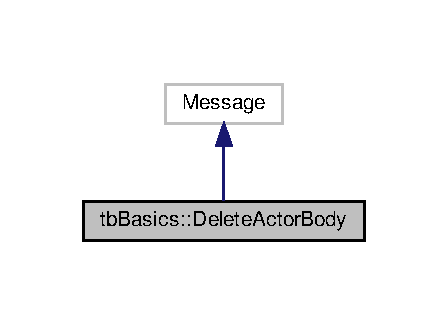
\includegraphics[width=215pt]{classtbBasics_1_1DeleteActorBody__inherit__graph}
\end{center}
\end{figure}


Collaboration diagram for tb\+Basics\+:\+:Delete\+Actor\+Body\+:
\nopagebreak
\begin{figure}[H]
\begin{center}
\leavevmode
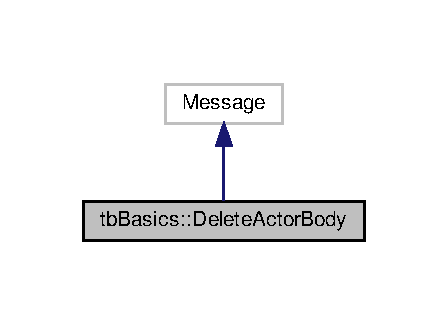
\includegraphics[width=215pt]{classtbBasics_1_1DeleteActorBody__coll__graph}
\end{center}
\end{figure}
\subsection*{Classes}
\begin{DoxyCompactItemize}
\item 
class \hyperlink{classtbBasics_1_1DeleteActorBody_1_1HasBitSetters}{Has\+Bit\+Setters}
\end{DoxyCompactItemize}
\subsection*{Public Member Functions}
\begin{DoxyCompactItemize}
\item 
\mbox{\Hypertarget{classtbBasics_1_1DeleteActorBody_accff4e03f84be0dd6e328c4b746296d9}\label{classtbBasics_1_1DeleteActorBody_accff4e03f84be0dd6e328c4b746296d9}} 
{\bfseries Delete\+Actor\+Body} (const \hyperlink{classtbBasics_1_1DeleteActorBody}{Delete\+Actor\+Body} \&from)
\item 
\mbox{\Hypertarget{classtbBasics_1_1DeleteActorBody_ab8118e7bfeb89b8e3bf1b40d923729c2}\label{classtbBasics_1_1DeleteActorBody_ab8118e7bfeb89b8e3bf1b40d923729c2}} 
\hyperlink{classtbBasics_1_1DeleteActorBody}{Delete\+Actor\+Body} \& {\bfseries operator=} (const \hyperlink{classtbBasics_1_1DeleteActorBody}{Delete\+Actor\+Body} \&from)
\item 
\mbox{\Hypertarget{classtbBasics_1_1DeleteActorBody_a5e0ab8c99b24c5b6b1429409b41b2286}\label{classtbBasics_1_1DeleteActorBody_a5e0ab8c99b24c5b6b1429409b41b2286}} 
void {\bfseries Swap} (\hyperlink{classtbBasics_1_1DeleteActorBody}{Delete\+Actor\+Body} $\ast$other)
\item 
\mbox{\Hypertarget{classtbBasics_1_1DeleteActorBody_a4018ec1e6951c0f9a8c0345ed4929710}\label{classtbBasics_1_1DeleteActorBody_a4018ec1e6951c0f9a8c0345ed4929710}} 
\hyperlink{classtbBasics_1_1DeleteActorBody}{Delete\+Actor\+Body} $\ast$ {\bfseries New} () const final
\item 
\mbox{\Hypertarget{classtbBasics_1_1DeleteActorBody_a2549f60a80839599a50ae4781c250ecc}\label{classtbBasics_1_1DeleteActorBody_a2549f60a80839599a50ae4781c250ecc}} 
\hyperlink{classtbBasics_1_1DeleteActorBody}{Delete\+Actor\+Body} $\ast$ {\bfseries New} (\+::google\+::protobuf\+::\+Arena $\ast$arena) const final
\item 
\mbox{\Hypertarget{classtbBasics_1_1DeleteActorBody_a8ea7c420a491d3c6279c85b1a14b4e68}\label{classtbBasics_1_1DeleteActorBody_a8ea7c420a491d3c6279c85b1a14b4e68}} 
void {\bfseries Copy\+From} (const \+::google\+::protobuf\+::\+Message \&from) final
\item 
\mbox{\Hypertarget{classtbBasics_1_1DeleteActorBody_a37588befa16fae702fdad8368f580ead}\label{classtbBasics_1_1DeleteActorBody_a37588befa16fae702fdad8368f580ead}} 
void {\bfseries Merge\+From} (const \+::google\+::protobuf\+::\+Message \&from) final
\item 
\mbox{\Hypertarget{classtbBasics_1_1DeleteActorBody_a3d2a9f2664ea9833030edad0c9abb8cf}\label{classtbBasics_1_1DeleteActorBody_a3d2a9f2664ea9833030edad0c9abb8cf}} 
void {\bfseries Copy\+From} (const \hyperlink{classtbBasics_1_1DeleteActorBody}{Delete\+Actor\+Body} \&from)
\item 
\mbox{\Hypertarget{classtbBasics_1_1DeleteActorBody_ae70bcc0fa8da86834c2bdd4797dc4587}\label{classtbBasics_1_1DeleteActorBody_ae70bcc0fa8da86834c2bdd4797dc4587}} 
void {\bfseries Merge\+From} (const \hyperlink{classtbBasics_1_1DeleteActorBody}{Delete\+Actor\+Body} \&from)
\item 
\mbox{\Hypertarget{classtbBasics_1_1DeleteActorBody_a34e8d6c8094704f073a0480472e6184a}\label{classtbBasics_1_1DeleteActorBody_a34e8d6c8094704f073a0480472e6184a}} 
P\+R\+O\+T\+O\+B\+U\+F\+\_\+\+A\+T\+T\+R\+I\+B\+U\+T\+E\+\_\+\+R\+E\+I\+N\+I\+T\+I\+A\+L\+I\+Z\+ES void {\bfseries Clear} () final
\item 
\mbox{\Hypertarget{classtbBasics_1_1DeleteActorBody_a37d0ed7bbc6044bb41f26c235f021acb}\label{classtbBasics_1_1DeleteActorBody_a37d0ed7bbc6044bb41f26c235f021acb}} 
bool {\bfseries Is\+Initialized} () const final
\item 
\mbox{\Hypertarget{classtbBasics_1_1DeleteActorBody_a44a787853a48cac514a6917b37094ddd}\label{classtbBasics_1_1DeleteActorBody_a44a787853a48cac514a6917b37094ddd}} 
size\+\_\+t {\bfseries Byte\+Size\+Long} () const final
\item 
\mbox{\Hypertarget{classtbBasics_1_1DeleteActorBody_a4f79c0df81861278c403e52a3f949d9b}\label{classtbBasics_1_1DeleteActorBody_a4f79c0df81861278c403e52a3f949d9b}} 
bool {\bfseries Merge\+Partial\+From\+Coded\+Stream} (\+::google\+::protobuf\+::io\+::\+Coded\+Input\+Stream $\ast$input) final
\item 
\mbox{\Hypertarget{classtbBasics_1_1DeleteActorBody_aee7f4ce560277c9466d3fb97d38af628}\label{classtbBasics_1_1DeleteActorBody_aee7f4ce560277c9466d3fb97d38af628}} 
void {\bfseries Serialize\+With\+Cached\+Sizes} (\+::google\+::protobuf\+::io\+::\+Coded\+Output\+Stream $\ast$output) const final
\item 
\mbox{\Hypertarget{classtbBasics_1_1DeleteActorBody_aa2f249fa48fa177247853a7da9c3045a}\label{classtbBasics_1_1DeleteActorBody_aa2f249fa48fa177247853a7da9c3045a}} 
\+::google\+::protobuf\+::uint8 $\ast$ {\bfseries Internal\+Serialize\+With\+Cached\+Sizes\+To\+Array} (\+::google\+::protobuf\+::uint8 $\ast$target) const final
\item 
\mbox{\Hypertarget{classtbBasics_1_1DeleteActorBody_a38e25d46b81eeca00895e42b6d95cb0f}\label{classtbBasics_1_1DeleteActorBody_a38e25d46b81eeca00895e42b6d95cb0f}} 
int {\bfseries Get\+Cached\+Size} () const final
\item 
\mbox{\Hypertarget{classtbBasics_1_1DeleteActorBody_abfb32cc3aed593a3e552f4ae78fb72ea}\label{classtbBasics_1_1DeleteActorBody_abfb32cc3aed593a3e552f4ae78fb72ea}} 
\+::google\+::protobuf\+::\+Metadata {\bfseries Get\+Metadata} () const final
\item 
\mbox{\Hypertarget{classtbBasics_1_1DeleteActorBody_a6d9d3d43f82d17ab4197fb9f4532d499}\label{classtbBasics_1_1DeleteActorBody_a6d9d3d43f82d17ab4197fb9f4532d499}} 
void {\bfseries clear\+\_\+id} ()
\item 
\mbox{\Hypertarget{classtbBasics_1_1DeleteActorBody_a78d4ec52e47da5b0c749d11880bd22bb}\label{classtbBasics_1_1DeleteActorBody_a78d4ec52e47da5b0c749d11880bd22bb}} 
\+::google\+::protobuf\+::uint32 {\bfseries id} () const
\item 
\mbox{\Hypertarget{classtbBasics_1_1DeleteActorBody_a2657a381b7395d0049039ecefded4f68}\label{classtbBasics_1_1DeleteActorBody_a2657a381b7395d0049039ecefded4f68}} 
void {\bfseries set\+\_\+id} (\+::google\+::protobuf\+::uint32 value)
\end{DoxyCompactItemize}
\subsection*{Static Public Member Functions}
\begin{DoxyCompactItemize}
\item 
\mbox{\Hypertarget{classtbBasics_1_1DeleteActorBody_aba075109825237a68de0f7d0000f4494}\label{classtbBasics_1_1DeleteActorBody_aba075109825237a68de0f7d0000f4494}} 
static const \+::google\+::protobuf\+::\+Descriptor $\ast$ {\bfseries descriptor} ()
\item 
\mbox{\Hypertarget{classtbBasics_1_1DeleteActorBody_a2c871e8f233879676e53e1338cd8c1b2}\label{classtbBasics_1_1DeleteActorBody_a2c871e8f233879676e53e1338cd8c1b2}} 
static const \hyperlink{classtbBasics_1_1DeleteActorBody}{Delete\+Actor\+Body} \& {\bfseries default\+\_\+instance} ()
\item 
\mbox{\Hypertarget{classtbBasics_1_1DeleteActorBody_ad16dab8ad538008a2a1b2a2a529f2b8c}\label{classtbBasics_1_1DeleteActorBody_ad16dab8ad538008a2a1b2a2a529f2b8c}} 
static void {\bfseries Init\+As\+Default\+Instance} ()
\item 
\mbox{\Hypertarget{classtbBasics_1_1DeleteActorBody_a875912c1e1aec71a617d25ad43a99001}\label{classtbBasics_1_1DeleteActorBody_a875912c1e1aec71a617d25ad43a99001}} 
static const \hyperlink{classtbBasics_1_1DeleteActorBody}{Delete\+Actor\+Body} $\ast$ {\bfseries internal\+\_\+default\+\_\+instance} ()
\end{DoxyCompactItemize}
\subsection*{Static Public Attributes}
\begin{DoxyCompactItemize}
\item 
static constexpr int {\bfseries k\+Index\+In\+File\+Messages}
\item 
\mbox{\Hypertarget{classtbBasics_1_1DeleteActorBody_abba916f1f94268d9728f7ae559111e0a}\label{classtbBasics_1_1DeleteActorBody_abba916f1f94268d9728f7ae559111e0a}} 
static const int {\bfseries k\+Id\+Field\+Number} = 1
\end{DoxyCompactItemize}
\subsection*{Friends}
\begin{DoxyCompactItemize}
\item 
\mbox{\Hypertarget{classtbBasics_1_1DeleteActorBody_ae86a2f4c520666b65d606ccbe2122e61}\label{classtbBasics_1_1DeleteActorBody_ae86a2f4c520666b65d606ccbe2122e61}} 
struct {\bfseries \+::\+Table\+Struct\+\_\+basic\+\_\+2eproto}
\item 
\mbox{\Hypertarget{classtbBasics_1_1DeleteActorBody_a7e7b4c032bd6b8ee75e5f56c267a03f0}\label{classtbBasics_1_1DeleteActorBody_a7e7b4c032bd6b8ee75e5f56c267a03f0}} 
void {\bfseries swap} (\hyperlink{classtbBasics_1_1DeleteActorBody}{Delete\+Actor\+Body} \&a, \hyperlink{classtbBasics_1_1DeleteActorBody}{Delete\+Actor\+Body} \&b)
\end{DoxyCompactItemize}


\subsection{Member Data Documentation}
\mbox{\Hypertarget{classtbBasics_1_1DeleteActorBody_a1219361ba785676c175587a3e12842f5}\label{classtbBasics_1_1DeleteActorBody_a1219361ba785676c175587a3e12842f5}} 
\index{tb\+Basics\+::\+Delete\+Actor\+Body@{tb\+Basics\+::\+Delete\+Actor\+Body}!k\+Index\+In\+File\+Messages@{k\+Index\+In\+File\+Messages}}
\index{k\+Index\+In\+File\+Messages@{k\+Index\+In\+File\+Messages}!tb\+Basics\+::\+Delete\+Actor\+Body@{tb\+Basics\+::\+Delete\+Actor\+Body}}
\subsubsection{\texorpdfstring{k\+Index\+In\+File\+Messages}{kIndexInFileMessages}}
{\footnotesize\ttfamily constexpr int tb\+Basics\+::\+Delete\+Actor\+Body\+::k\+Index\+In\+File\+Messages\hspace{0.3cm}{\ttfamily [static]}}

{\bfseries Initial value\+:}
\begin{DoxyCode}
=
    1
\end{DoxyCode}


The documentation for this class was generated from the following files\+:\begin{DoxyCompactItemize}
\item 
Tarbora/\+Messages/proto/basic.\+pb.\+h\item 
Tarbora/\+Messages/proto/basic.\+pb.\+cc\end{DoxyCompactItemize}

\hypertarget{classtbBasics_1_1DeleteActorBodyDefaultTypeInternal}{}\section{tb\+Basics\+:\+:Delete\+Actor\+Body\+Default\+Type\+Internal Class Reference}
\label{classtbBasics_1_1DeleteActorBodyDefaultTypeInternal}\index{tb\+Basics\+::\+Delete\+Actor\+Body\+Default\+Type\+Internal@{tb\+Basics\+::\+Delete\+Actor\+Body\+Default\+Type\+Internal}}
\subsection*{Public Attributes}
\begin{DoxyCompactItemize}
\item 
\mbox{\Hypertarget{classtbBasics_1_1DeleteActorBodyDefaultTypeInternal_a9849e40231a4c4887de49bcb323b4b06}\label{classtbBasics_1_1DeleteActorBodyDefaultTypeInternal_a9849e40231a4c4887de49bcb323b4b06}} 
\+::google\+::protobuf\+::internal\+::\+Explicitly\+Constructed$<$ \hyperlink{classtbBasics_1_1DeleteActorBody}{Delete\+Actor\+Body} $>$ {\bfseries \+\_\+instance}
\end{DoxyCompactItemize}


The documentation for this class was generated from the following file\+:\begin{DoxyCompactItemize}
\item 
Tarbora/\+Messages/proto/basic.\+pb.\+cc\end{DoxyCompactItemize}

\hypertarget{classTarbora_1_1DemoWindow}{}\section{Tarbora\+:\+:Demo\+Window Class Reference}
\label{classTarbora_1_1DemoWindow}\index{Tarbora\+::\+Demo\+Window@{Tarbora\+::\+Demo\+Window}}


Inheritance diagram for Tarbora\+:\+:Demo\+Window\+:
\nopagebreak
\begin{figure}[H]
\begin{center}
\leavevmode
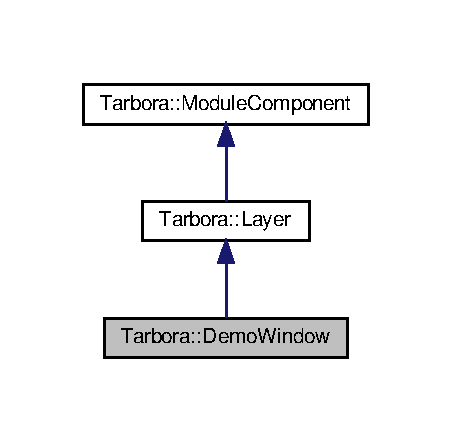
\includegraphics[width=217pt]{classTarbora_1_1DemoWindow__inherit__graph}
\end{center}
\end{figure}


Collaboration diagram for Tarbora\+:\+:Demo\+Window\+:
\nopagebreak
\begin{figure}[H]
\begin{center}
\leavevmode
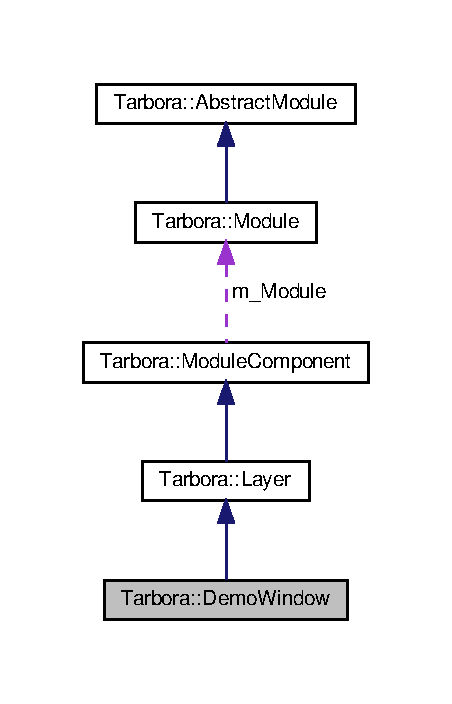
\includegraphics[width=217pt]{classTarbora_1_1DemoWindow__coll__graph}
\end{center}
\end{figure}
\subsection*{Public Member Functions}
\begin{DoxyCompactItemize}
\item 
\mbox{\Hypertarget{classTarbora_1_1DemoWindow_a20c62ad3f1602152c50efcb1e2c3b16d}\label{classTarbora_1_1DemoWindow_a20c62ad3f1602152c50efcb1e2c3b16d}} 
{\bfseries Demo\+Window} (\hyperlink{classTarbora_1_1GraphicView}{Graphic\+View} $\ast$view, bool start\+\_\+active)
\item 
\mbox{\Hypertarget{classTarbora_1_1DemoWindow_a8537497b035002c4adcf3c2ab97069f1}\label{classTarbora_1_1DemoWindow_a8537497b035002c4adcf3c2ab97069f1}} 
void {\bfseries get\+Input} () override
\item 
\mbox{\Hypertarget{classTarbora_1_1DemoWindow_a88b0354686e440a7bd783ccf33dafe6a}\label{classTarbora_1_1DemoWindow_a88b0354686e440a7bd783ccf33dafe6a}} 
void {\bfseries draw} () override
\end{DoxyCompactItemize}
\subsection*{Additional Inherited Members}


The documentation for this class was generated from the following file\+:\begin{DoxyCompactItemize}
\item 
Tarbora/\+Views/\+Graphic\+Views/Demo\+Window.\+hpp\end{DoxyCompactItemize}

\hypertarget{classtbMessages_1_1Empty}{}\section{tb\+Messages\+:\+:Empty Class Reference}
\label{classtbMessages_1_1Empty}\index{tb\+Messages\+::\+Empty@{tb\+Messages\+::\+Empty}}


Inheritance diagram for tb\+Messages\+:\+:Empty\+:
\nopagebreak
\begin{figure}[H]
\begin{center}
\leavevmode
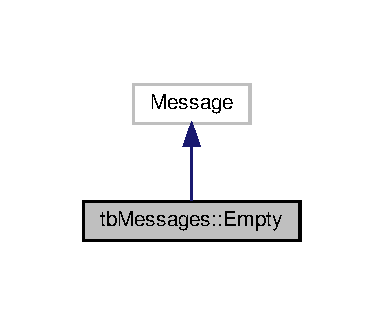
\includegraphics[width=184pt]{classtbMessages_1_1Empty__inherit__graph}
\end{center}
\end{figure}


Collaboration diagram for tb\+Messages\+:\+:Empty\+:
\nopagebreak
\begin{figure}[H]
\begin{center}
\leavevmode
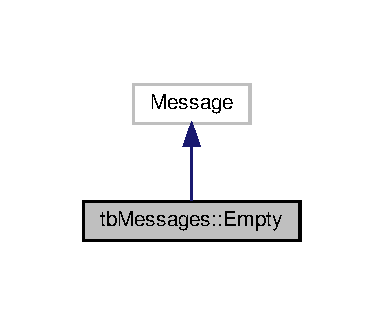
\includegraphics[width=184pt]{classtbMessages_1_1Empty__coll__graph}
\end{center}
\end{figure}
\subsection*{Classes}
\begin{DoxyCompactItemize}
\item 
class \hyperlink{classtbMessages_1_1Empty_1_1HasBitSetters}{Has\+Bit\+Setters}
\end{DoxyCompactItemize}
\subsection*{Public Member Functions}
\begin{DoxyCompactItemize}
\item 
\mbox{\Hypertarget{classtbMessages_1_1Empty_aa7824763efec590a17437da6c6cb8d41}\label{classtbMessages_1_1Empty_aa7824763efec590a17437da6c6cb8d41}} 
{\bfseries Empty} (const \hyperlink{classtbMessages_1_1Empty}{Empty} \&from)
\item 
\mbox{\Hypertarget{classtbMessages_1_1Empty_a9df5a6b35aa1d3a8ff4284985182ec42}\label{classtbMessages_1_1Empty_a9df5a6b35aa1d3a8ff4284985182ec42}} 
\hyperlink{classtbMessages_1_1Empty}{Empty} \& {\bfseries operator=} (const \hyperlink{classtbMessages_1_1Empty}{Empty} \&from)
\item 
\mbox{\Hypertarget{classtbMessages_1_1Empty_a08f7cbbdf9e391436eff4aca0b0aa43b}\label{classtbMessages_1_1Empty_a08f7cbbdf9e391436eff4aca0b0aa43b}} 
void {\bfseries Swap} (\hyperlink{classtbMessages_1_1Empty}{Empty} $\ast$other)
\item 
\mbox{\Hypertarget{classtbMessages_1_1Empty_a1edf25524dc0b215485563923dbbc258}\label{classtbMessages_1_1Empty_a1edf25524dc0b215485563923dbbc258}} 
\hyperlink{classtbMessages_1_1Empty}{Empty} $\ast$ {\bfseries New} () const final
\item 
\mbox{\Hypertarget{classtbMessages_1_1Empty_a91ff2ecd77c42cd59a84c574e60669b2}\label{classtbMessages_1_1Empty_a91ff2ecd77c42cd59a84c574e60669b2}} 
\hyperlink{classtbMessages_1_1Empty}{Empty} $\ast$ {\bfseries New} (\+::google\+::protobuf\+::\+Arena $\ast$arena) const final
\item 
\mbox{\Hypertarget{classtbMessages_1_1Empty_adad5aecdaf0cece96f43f5d672a26712}\label{classtbMessages_1_1Empty_adad5aecdaf0cece96f43f5d672a26712}} 
void {\bfseries Copy\+From} (const \+::google\+::protobuf\+::\+Message \&from) final
\item 
\mbox{\Hypertarget{classtbMessages_1_1Empty_a018730b17c2c39ebdd83cd72f9ea8e1f}\label{classtbMessages_1_1Empty_a018730b17c2c39ebdd83cd72f9ea8e1f}} 
void {\bfseries Merge\+From} (const \+::google\+::protobuf\+::\+Message \&from) final
\item 
\mbox{\Hypertarget{classtbMessages_1_1Empty_a0f6385ced7a0b262507e8803bcafecef}\label{classtbMessages_1_1Empty_a0f6385ced7a0b262507e8803bcafecef}} 
void {\bfseries Copy\+From} (const \hyperlink{classtbMessages_1_1Empty}{Empty} \&from)
\item 
\mbox{\Hypertarget{classtbMessages_1_1Empty_a701838ecf826fbc48eccfac06de42542}\label{classtbMessages_1_1Empty_a701838ecf826fbc48eccfac06de42542}} 
void {\bfseries Merge\+From} (const \hyperlink{classtbMessages_1_1Empty}{Empty} \&from)
\item 
\mbox{\Hypertarget{classtbMessages_1_1Empty_a36881810a97d00b2e8761b12f979376b}\label{classtbMessages_1_1Empty_a36881810a97d00b2e8761b12f979376b}} 
P\+R\+O\+T\+O\+B\+U\+F\+\_\+\+A\+T\+T\+R\+I\+B\+U\+T\+E\+\_\+\+R\+E\+I\+N\+I\+T\+I\+A\+L\+I\+Z\+ES void {\bfseries Clear} () final
\item 
\mbox{\Hypertarget{classtbMessages_1_1Empty_a2c5df2b03499c3cd4aa9c149269a5313}\label{classtbMessages_1_1Empty_a2c5df2b03499c3cd4aa9c149269a5313}} 
bool {\bfseries Is\+Initialized} () const final
\item 
\mbox{\Hypertarget{classtbMessages_1_1Empty_a570a9269152154ba74eaf2803f5a1cd9}\label{classtbMessages_1_1Empty_a570a9269152154ba74eaf2803f5a1cd9}} 
size\+\_\+t {\bfseries Byte\+Size\+Long} () const final
\item 
\mbox{\Hypertarget{classtbMessages_1_1Empty_a9efaca91b96abb8b7da28e3e148a9de2}\label{classtbMessages_1_1Empty_a9efaca91b96abb8b7da28e3e148a9de2}} 
bool {\bfseries Merge\+Partial\+From\+Coded\+Stream} (\+::google\+::protobuf\+::io\+::\+Coded\+Input\+Stream $\ast$input) final
\item 
\mbox{\Hypertarget{classtbMessages_1_1Empty_a3a49e1903f404bb7792cfee9c8be7062}\label{classtbMessages_1_1Empty_a3a49e1903f404bb7792cfee9c8be7062}} 
void {\bfseries Serialize\+With\+Cached\+Sizes} (\+::google\+::protobuf\+::io\+::\+Coded\+Output\+Stream $\ast$output) const final
\item 
\mbox{\Hypertarget{classtbMessages_1_1Empty_a0725ec9dcc4b3586e07d95f1736f961e}\label{classtbMessages_1_1Empty_a0725ec9dcc4b3586e07d95f1736f961e}} 
\+::google\+::protobuf\+::uint8 $\ast$ {\bfseries Internal\+Serialize\+With\+Cached\+Sizes\+To\+Array} (\+::google\+::protobuf\+::uint8 $\ast$target) const final
\item 
\mbox{\Hypertarget{classtbMessages_1_1Empty_ac563d246a710f6a7c71e1861909275cb}\label{classtbMessages_1_1Empty_ac563d246a710f6a7c71e1861909275cb}} 
int {\bfseries Get\+Cached\+Size} () const final
\item 
\mbox{\Hypertarget{classtbMessages_1_1Empty_ade840f4ac2ef51c5821d683c70e9a843}\label{classtbMessages_1_1Empty_ade840f4ac2ef51c5821d683c70e9a843}} 
\+::google\+::protobuf\+::\+Metadata {\bfseries Get\+Metadata} () const final
\end{DoxyCompactItemize}
\subsection*{Static Public Member Functions}
\begin{DoxyCompactItemize}
\item 
\mbox{\Hypertarget{classtbMessages_1_1Empty_a4ce4c33a1420ad1d4618898c739544f6}\label{classtbMessages_1_1Empty_a4ce4c33a1420ad1d4618898c739544f6}} 
static const \+::google\+::protobuf\+::\+Descriptor $\ast$ {\bfseries descriptor} ()
\item 
\mbox{\Hypertarget{classtbMessages_1_1Empty_aa8fd3af296539738b97b9f00d6e30ec6}\label{classtbMessages_1_1Empty_aa8fd3af296539738b97b9f00d6e30ec6}} 
static const \hyperlink{classtbMessages_1_1Empty}{Empty} \& {\bfseries default\+\_\+instance} ()
\item 
\mbox{\Hypertarget{classtbMessages_1_1Empty_ae2989c73d47aa01f3c39e7382c0a181d}\label{classtbMessages_1_1Empty_ae2989c73d47aa01f3c39e7382c0a181d}} 
static void {\bfseries Init\+As\+Default\+Instance} ()
\item 
\mbox{\Hypertarget{classtbMessages_1_1Empty_a4c31dee39671e45833f38972bfcdbacc}\label{classtbMessages_1_1Empty_a4c31dee39671e45833f38972bfcdbacc}} 
static const \hyperlink{classtbMessages_1_1Empty}{Empty} $\ast$ {\bfseries internal\+\_\+default\+\_\+instance} ()
\end{DoxyCompactItemize}
\subsection*{Static Public Attributes}
\begin{DoxyCompactItemize}
\item 
static constexpr int {\bfseries k\+Index\+In\+File\+Messages}
\end{DoxyCompactItemize}
\subsection*{Friends}
\begin{DoxyCompactItemize}
\item 
\mbox{\Hypertarget{classtbMessages_1_1Empty_a6669c254757d8a4b2e1f51c0da62dd91}\label{classtbMessages_1_1Empty_a6669c254757d8a4b2e1f51c0da62dd91}} 
struct {\bfseries \+::\+Table\+Struct\+\_\+messages\+\_\+2eproto}
\item 
\mbox{\Hypertarget{classtbMessages_1_1Empty_aa89f86120de5aa1f2151023feca8458e}\label{classtbMessages_1_1Empty_aa89f86120de5aa1f2151023feca8458e}} 
void {\bfseries swap} (\hyperlink{classtbMessages_1_1Empty}{Empty} \&a, \hyperlink{classtbMessages_1_1Empty}{Empty} \&b)
\end{DoxyCompactItemize}


\subsection{Member Data Documentation}
\mbox{\Hypertarget{classtbMessages_1_1Empty_afb6c4379d22cec14b098090dc97b919a}\label{classtbMessages_1_1Empty_afb6c4379d22cec14b098090dc97b919a}} 
\index{tb\+Messages\+::\+Empty@{tb\+Messages\+::\+Empty}!k\+Index\+In\+File\+Messages@{k\+Index\+In\+File\+Messages}}
\index{k\+Index\+In\+File\+Messages@{k\+Index\+In\+File\+Messages}!tb\+Messages\+::\+Empty@{tb\+Messages\+::\+Empty}}
\subsubsection{\texorpdfstring{k\+Index\+In\+File\+Messages}{kIndexInFileMessages}}
{\footnotesize\ttfamily constexpr int tb\+Messages\+::\+Empty\+::k\+Index\+In\+File\+Messages\hspace{0.3cm}{\ttfamily [static]}}

{\bfseries Initial value\+:}
\begin{DoxyCode}
=
    2
\end{DoxyCode}


The documentation for this class was generated from the following files\+:\begin{DoxyCompactItemize}
\item 
Tarbora/\+Framework/\+Protos/messages.\+pb.\+h\item 
Tarbora/\+Framework/\+Protos/messages.\+pb.\+cc\end{DoxyCompactItemize}

\hypertarget{classTarbora_1_1EmptyComponent}{}\section{Tarbora\+:\+:Empty\+Component Class Reference}
\label{classTarbora_1_1EmptyComponent}\index{Tarbora\+::\+Empty\+Component@{Tarbora\+::\+Empty\+Component}}


Inheritance diagram for Tarbora\+:\+:Empty\+Component\+:
\nopagebreak
\begin{figure}[H]
\begin{center}
\leavevmode
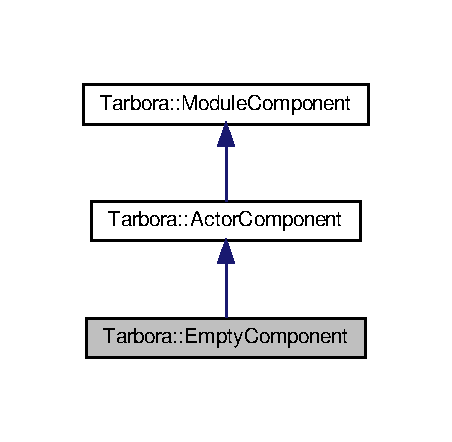
\includegraphics[width=217pt]{classTarbora_1_1EmptyComponent__inherit__graph}
\end{center}
\end{figure}


Collaboration diagram for Tarbora\+:\+:Empty\+Component\+:
\nopagebreak
\begin{figure}[H]
\begin{center}
\leavevmode
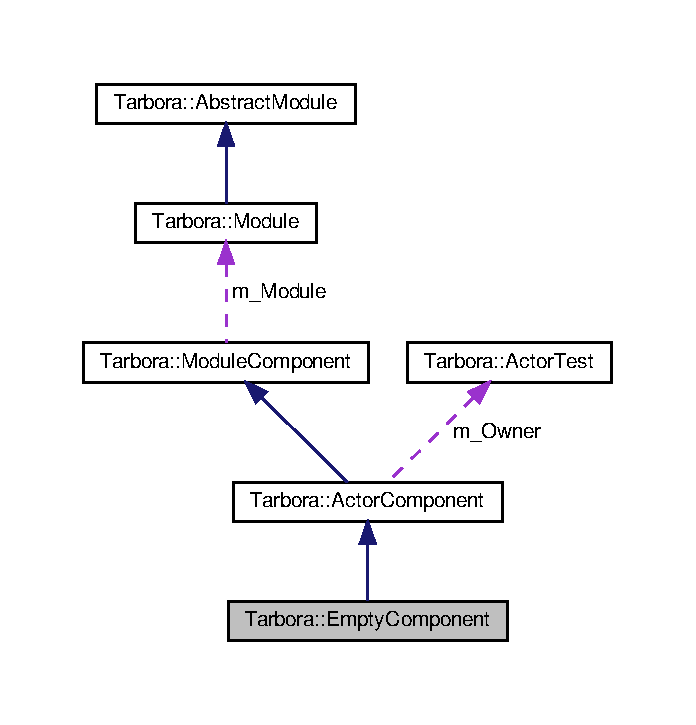
\includegraphics[width=334pt]{classTarbora_1_1EmptyComponent__coll__graph}
\end{center}
\end{figure}
\subsection*{Public Member Functions}
\begin{DoxyCompactItemize}
\item 
\mbox{\Hypertarget{classTarbora_1_1EmptyComponent_a1d7d043e5bc46e44c0f6eac1bb3990c3}\label{classTarbora_1_1EmptyComponent_a1d7d043e5bc46e44c0f6eac1bb3990c3}} 
{\bfseries Empty\+Component} (\hyperlink{classTarbora_1_1World}{World} $\ast$world)
\item 
\mbox{\Hypertarget{classTarbora_1_1EmptyComponent_ae3c9b5e69b060f82b73fb4e467fb0498}\label{classTarbora_1_1EmptyComponent_ae3c9b5e69b060f82b73fb4e467fb0498}} 
bool {\bfseries Init} (Json\+Ptr resource, raw\+\_\+json data)
\item 
\mbox{\Hypertarget{classTarbora_1_1EmptyComponent_a029c567c28635d6342038a44ff75d59f}\label{classTarbora_1_1EmptyComponent_a029c567c28635d6342038a44ff75d59f}} 
Component\+Id {\bfseries Get\+Id} () const
\end{DoxyCompactItemize}
\subsection*{Static Public Member Functions}
\begin{DoxyCompactItemize}
\item 
\mbox{\Hypertarget{classTarbora_1_1EmptyComponent_ad7f0e222ad2aee4729190ee3b701b156}\label{classTarbora_1_1EmptyComponent_ad7f0e222ad2aee4729190ee3b701b156}} 
static Actor\+Component\+Ptr {\bfseries Creator} (\hyperlink{classTarbora_1_1World}{World} $\ast$world)
\end{DoxyCompactItemize}
\subsection*{Additional Inherited Members}


The documentation for this class was generated from the following file\+:\begin{DoxyCompactItemize}
\item 
Tarbora/\+Logic/inc/Components.\+hpp\end{DoxyCompactItemize}

\hypertarget{classtbMessages_1_1EmptyDefaultTypeInternal}{}\section{tb\+Messages\+:\+:Empty\+Default\+Type\+Internal Class Reference}
\label{classtbMessages_1_1EmptyDefaultTypeInternal}\index{tb\+Messages\+::\+Empty\+Default\+Type\+Internal@{tb\+Messages\+::\+Empty\+Default\+Type\+Internal}}
\subsection*{Public Attributes}
\begin{DoxyCompactItemize}
\item 
\mbox{\Hypertarget{classtbMessages_1_1EmptyDefaultTypeInternal_ab86b0f872d49ea95442d6919ad65465a}\label{classtbMessages_1_1EmptyDefaultTypeInternal_ab86b0f872d49ea95442d6919ad65465a}} 
\+::google\+::protobuf\+::internal\+::\+Explicitly\+Constructed$<$ \hyperlink{classtbMessages_1_1Empty}{Empty} $>$ {\bfseries \+\_\+instance}
\end{DoxyCompactItemize}


The documentation for this class was generated from the following file\+:\begin{DoxyCompactItemize}
\item 
Tarbora/\+Framework/\+Protos/messages.\+pb.\+cc\end{DoxyCompactItemize}

\hypertarget{classtbMessages_1_1EventHeader}{}\section{tb\+Messages\+:\+:Event\+Header Class Reference}
\label{classtbMessages_1_1EventHeader}\index{tb\+Messages\+::\+Event\+Header@{tb\+Messages\+::\+Event\+Header}}


Inheritance diagram for tb\+Messages\+:\+:Event\+Header\+:
\nopagebreak
\begin{figure}[H]
\begin{center}
\leavevmode
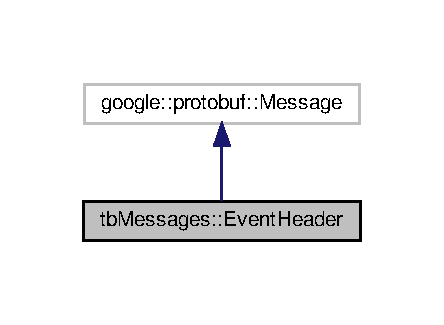
\includegraphics[width=213pt]{classtbMessages_1_1EventHeader__inherit__graph}
\end{center}
\end{figure}


Collaboration diagram for tb\+Messages\+:\+:Event\+Header\+:
\nopagebreak
\begin{figure}[H]
\begin{center}
\leavevmode
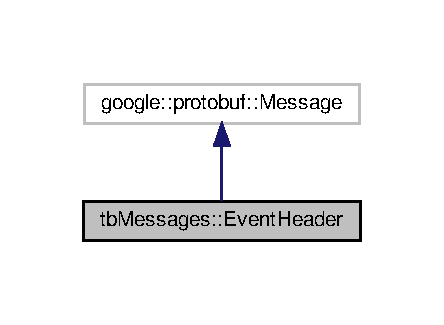
\includegraphics[width=213pt]{classtbMessages_1_1EventHeader__coll__graph}
\end{center}
\end{figure}
\subsection*{Classes}
\begin{DoxyCompactItemize}
\item 
class \hyperlink{classtbMessages_1_1EventHeader_1_1HasBitSetters}{Has\+Bit\+Setters}
\end{DoxyCompactItemize}
\subsection*{Public Member Functions}
\begin{DoxyCompactItemize}
\item 
\mbox{\Hypertarget{classtbMessages_1_1EventHeader_adba34308e967b4a5053b242501ef8c53}\label{classtbMessages_1_1EventHeader_adba34308e967b4a5053b242501ef8c53}} 
{\bfseries Event\+Header} (const \hyperlink{classtbMessages_1_1EventHeader}{Event\+Header} \&from)
\item 
\mbox{\Hypertarget{classtbMessages_1_1EventHeader_a28cb21111a16edececa80f612a05d520}\label{classtbMessages_1_1EventHeader_a28cb21111a16edececa80f612a05d520}} 
\hyperlink{classtbMessages_1_1EventHeader}{Event\+Header} \& {\bfseries operator=} (const \hyperlink{classtbMessages_1_1EventHeader}{Event\+Header} \&from)
\item 
\mbox{\Hypertarget{classtbMessages_1_1EventHeader_adb57d9d23f67c03289729e9e9c3652a8}\label{classtbMessages_1_1EventHeader_adb57d9d23f67c03289729e9e9c3652a8}} 
void {\bfseries Swap} (\hyperlink{classtbMessages_1_1EventHeader}{Event\+Header} $\ast$other)
\item 
\mbox{\Hypertarget{classtbMessages_1_1EventHeader_ac5a9d2eb2141e28323f0997df801fddd}\label{classtbMessages_1_1EventHeader_ac5a9d2eb2141e28323f0997df801fddd}} 
\hyperlink{classtbMessages_1_1EventHeader}{Event\+Header} $\ast$ {\bfseries New} () const final
\item 
\mbox{\Hypertarget{classtbMessages_1_1EventHeader_ab69a6498ef99f793bfed5a5967a89841}\label{classtbMessages_1_1EventHeader_ab69a6498ef99f793bfed5a5967a89841}} 
\hyperlink{classtbMessages_1_1EventHeader}{Event\+Header} $\ast$ {\bfseries New} (\+::google\+::protobuf\+::\+Arena $\ast$arena) const final
\item 
\mbox{\Hypertarget{classtbMessages_1_1EventHeader_adc7f02971e204c36c27f154b64becd83}\label{classtbMessages_1_1EventHeader_adc7f02971e204c36c27f154b64becd83}} 
void {\bfseries Copy\+From} (const \+::google\+::protobuf\+::\+Message \&from) final
\item 
\mbox{\Hypertarget{classtbMessages_1_1EventHeader_a24cf60e38d59fbaeb673efb87c0834e6}\label{classtbMessages_1_1EventHeader_a24cf60e38d59fbaeb673efb87c0834e6}} 
void {\bfseries Merge\+From} (const \+::google\+::protobuf\+::\+Message \&from) final
\item 
\mbox{\Hypertarget{classtbMessages_1_1EventHeader_aa5bc5d5fcff70cf341521f9958614d2d}\label{classtbMessages_1_1EventHeader_aa5bc5d5fcff70cf341521f9958614d2d}} 
void {\bfseries Copy\+From} (const \hyperlink{classtbMessages_1_1EventHeader}{Event\+Header} \&from)
\item 
\mbox{\Hypertarget{classtbMessages_1_1EventHeader_a520c2e734344e515ee034f11ce66b95c}\label{classtbMessages_1_1EventHeader_a520c2e734344e515ee034f11ce66b95c}} 
void {\bfseries Merge\+From} (const \hyperlink{classtbMessages_1_1EventHeader}{Event\+Header} \&from)
\item 
\mbox{\Hypertarget{classtbMessages_1_1EventHeader_ac63895e2fa84d4244d727431c621bd26}\label{classtbMessages_1_1EventHeader_ac63895e2fa84d4244d727431c621bd26}} 
P\+R\+O\+T\+O\+B\+U\+F\+\_\+\+A\+T\+T\+R\+I\+B\+U\+T\+E\+\_\+\+R\+E\+I\+N\+I\+T\+I\+A\+L\+I\+Z\+ES void {\bfseries Clear} () final
\item 
\mbox{\Hypertarget{classtbMessages_1_1EventHeader_aa3c5bbdd6a225251d7832f1ae953aa37}\label{classtbMessages_1_1EventHeader_aa3c5bbdd6a225251d7832f1ae953aa37}} 
bool {\bfseries Is\+Initialized} () const final
\item 
\mbox{\Hypertarget{classtbMessages_1_1EventHeader_abce3a7782847370045c64d7c0f3052e4}\label{classtbMessages_1_1EventHeader_abce3a7782847370045c64d7c0f3052e4}} 
size\+\_\+t {\bfseries Byte\+Size\+Long} () const final
\item 
\mbox{\Hypertarget{classtbMessages_1_1EventHeader_ace229166ac64a34a9673581354d7bd7a}\label{classtbMessages_1_1EventHeader_ace229166ac64a34a9673581354d7bd7a}} 
bool {\bfseries Merge\+Partial\+From\+Coded\+Stream} (\+::google\+::protobuf\+::io\+::\+Coded\+Input\+Stream $\ast$input) final
\item 
\mbox{\Hypertarget{classtbMessages_1_1EventHeader_a0d4efb9e81d34df4262bfbc28b8212d5}\label{classtbMessages_1_1EventHeader_a0d4efb9e81d34df4262bfbc28b8212d5}} 
void {\bfseries Serialize\+With\+Cached\+Sizes} (\+::google\+::protobuf\+::io\+::\+Coded\+Output\+Stream $\ast$output) const final
\item 
\mbox{\Hypertarget{classtbMessages_1_1EventHeader_a9dd7be02a38c7e494e682f6dd68584bf}\label{classtbMessages_1_1EventHeader_a9dd7be02a38c7e494e682f6dd68584bf}} 
\+::google\+::protobuf\+::uint8 $\ast$ {\bfseries Internal\+Serialize\+With\+Cached\+Sizes\+To\+Array} (\+::google\+::protobuf\+::uint8 $\ast$target) const final
\item 
\mbox{\Hypertarget{classtbMessages_1_1EventHeader_a430fb7822628cbfd7b385ffe01e85019}\label{classtbMessages_1_1EventHeader_a430fb7822628cbfd7b385ffe01e85019}} 
int {\bfseries Get\+Cached\+Size} () const final
\item 
\mbox{\Hypertarget{classtbMessages_1_1EventHeader_abe01d0cbdfc158051aa831db26a067de}\label{classtbMessages_1_1EventHeader_abe01d0cbdfc158051aa831db26a067de}} 
\+::google\+::protobuf\+::\+Metadata {\bfseries Get\+Metadata} () const final
\item 
\mbox{\Hypertarget{classtbMessages_1_1EventHeader_aa90b8b663c76d024a7e8df3d4728e000}\label{classtbMessages_1_1EventHeader_aa90b8b663c76d024a7e8df3d4728e000}} 
void {\bfseries clear\+\_\+subject} ()
\item 
\mbox{\Hypertarget{classtbMessages_1_1EventHeader_ab69dd04f481ee3f98729168ea40ffccb}\label{classtbMessages_1_1EventHeader_ab69dd04f481ee3f98729168ea40ffccb}} 
const \+::std\+::string \& {\bfseries subject} () const
\item 
\mbox{\Hypertarget{classtbMessages_1_1EventHeader_aa3c9e507218035d84203a8e52d8d7d84}\label{classtbMessages_1_1EventHeader_aa3c9e507218035d84203a8e52d8d7d84}} 
void {\bfseries set\+\_\+subject} (const \+::std\+::string \&value)
\item 
\mbox{\Hypertarget{classtbMessages_1_1EventHeader_a8d7ff8cb81d7c78884b13a4c539b2b27}\label{classtbMessages_1_1EventHeader_a8d7ff8cb81d7c78884b13a4c539b2b27}} 
void {\bfseries set\+\_\+subject} (const char $\ast$value)
\item 
\mbox{\Hypertarget{classtbMessages_1_1EventHeader_a2244e3a9230ca7991b17b95d05b7dcf3}\label{classtbMessages_1_1EventHeader_a2244e3a9230ca7991b17b95d05b7dcf3}} 
void {\bfseries set\+\_\+subject} (const char $\ast$value, size\+\_\+t size)
\item 
\mbox{\Hypertarget{classtbMessages_1_1EventHeader_a6bfe11181e0e2271f393df61792784c5}\label{classtbMessages_1_1EventHeader_a6bfe11181e0e2271f393df61792784c5}} 
\+::std\+::string $\ast$ {\bfseries mutable\+\_\+subject} ()
\item 
\mbox{\Hypertarget{classtbMessages_1_1EventHeader_aaf7af283586ca60ce3078060290cb6ee}\label{classtbMessages_1_1EventHeader_aaf7af283586ca60ce3078060290cb6ee}} 
\+::std\+::string $\ast$ {\bfseries release\+\_\+subject} ()
\item 
\mbox{\Hypertarget{classtbMessages_1_1EventHeader_a36b1b6bc030d78363ae3308c27963731}\label{classtbMessages_1_1EventHeader_a36b1b6bc030d78363ae3308c27963731}} 
void {\bfseries set\+\_\+allocated\+\_\+subject} (\+::std\+::string $\ast$subject)
\item 
\mbox{\Hypertarget{classtbMessages_1_1EventHeader_a7c723b88f169669dfa027795e70b1281}\label{classtbMessages_1_1EventHeader_a7c723b88f169669dfa027795e70b1281}} 
void {\bfseries clear\+\_\+from} ()
\item 
\mbox{\Hypertarget{classtbMessages_1_1EventHeader_a69f4664b3d1af4f3a456f811508861e0}\label{classtbMessages_1_1EventHeader_a69f4664b3d1af4f3a456f811508861e0}} 
\+::google\+::protobuf\+::int32 {\bfseries from} () const
\item 
\mbox{\Hypertarget{classtbMessages_1_1EventHeader_ac255d0989af7d1eee2c32affaaf7cec4}\label{classtbMessages_1_1EventHeader_ac255d0989af7d1eee2c32affaaf7cec4}} 
void {\bfseries set\+\_\+from} (\+::google\+::protobuf\+::int32 value)
\end{DoxyCompactItemize}
\subsection*{Static Public Member Functions}
\begin{DoxyCompactItemize}
\item 
\mbox{\Hypertarget{classtbMessages_1_1EventHeader_a51c722355d1fca67b1024733dca9f09f}\label{classtbMessages_1_1EventHeader_a51c722355d1fca67b1024733dca9f09f}} 
static const \+::google\+::protobuf\+::\+Descriptor $\ast$ {\bfseries descriptor} ()
\item 
\mbox{\Hypertarget{classtbMessages_1_1EventHeader_a982ba383994bad24976a728c7ad05d7d}\label{classtbMessages_1_1EventHeader_a982ba383994bad24976a728c7ad05d7d}} 
static const \hyperlink{classtbMessages_1_1EventHeader}{Event\+Header} \& {\bfseries default\+\_\+instance} ()
\item 
\mbox{\Hypertarget{classtbMessages_1_1EventHeader_a6c8a08cf9a5435ae931f3153175a6313}\label{classtbMessages_1_1EventHeader_a6c8a08cf9a5435ae931f3153175a6313}} 
static void {\bfseries Init\+As\+Default\+Instance} ()
\item 
\mbox{\Hypertarget{classtbMessages_1_1EventHeader_a8fbebeceada7a125db4e32699c24e502}\label{classtbMessages_1_1EventHeader_a8fbebeceada7a125db4e32699c24e502}} 
static const \hyperlink{classtbMessages_1_1EventHeader}{Event\+Header} $\ast$ {\bfseries internal\+\_\+default\+\_\+instance} ()
\end{DoxyCompactItemize}
\subsection*{Static Public Attributes}
\begin{DoxyCompactItemize}
\item 
static constexpr int {\bfseries k\+Index\+In\+File\+Messages}
\item 
\mbox{\Hypertarget{classtbMessages_1_1EventHeader_a457b78f3b7ed3d1bb9996c673bd8c000}\label{classtbMessages_1_1EventHeader_a457b78f3b7ed3d1bb9996c673bd8c000}} 
static const int {\bfseries k\+Subject\+Field\+Number} = 2
\item 
\mbox{\Hypertarget{classtbMessages_1_1EventHeader_aaaff3c6ee88e9f74bc13cecce1e63f26}\label{classtbMessages_1_1EventHeader_aaaff3c6ee88e9f74bc13cecce1e63f26}} 
static const int {\bfseries k\+From\+Field\+Number} = 1
\end{DoxyCompactItemize}
\subsection*{Friends}
\begin{DoxyCompactItemize}
\item 
\mbox{\Hypertarget{classtbMessages_1_1EventHeader_a6669c254757d8a4b2e1f51c0da62dd91}\label{classtbMessages_1_1EventHeader_a6669c254757d8a4b2e1f51c0da62dd91}} 
struct {\bfseries \+::\+Table\+Struct\+\_\+messages\+\_\+2eproto}
\item 
\mbox{\Hypertarget{classtbMessages_1_1EventHeader_acab06b4543eff02e693bc24fde842b89}\label{classtbMessages_1_1EventHeader_acab06b4543eff02e693bc24fde842b89}} 
void {\bfseries swap} (\hyperlink{classtbMessages_1_1EventHeader}{Event\+Header} \&a, \hyperlink{classtbMessages_1_1EventHeader}{Event\+Header} \&b)
\end{DoxyCompactItemize}


\subsection{Member Data Documentation}
\mbox{\Hypertarget{classtbMessages_1_1EventHeader_aff474cd410d29d094e15aff461a3a6bc}\label{classtbMessages_1_1EventHeader_aff474cd410d29d094e15aff461a3a6bc}} 
\index{tb\+Messages\+::\+Event\+Header@{tb\+Messages\+::\+Event\+Header}!k\+Index\+In\+File\+Messages@{k\+Index\+In\+File\+Messages}}
\index{k\+Index\+In\+File\+Messages@{k\+Index\+In\+File\+Messages}!tb\+Messages\+::\+Event\+Header@{tb\+Messages\+::\+Event\+Header}}
\subsubsection{\texorpdfstring{k\+Index\+In\+File\+Messages}{kIndexInFileMessages}}
{\footnotesize\ttfamily constexpr int tb\+Messages\+::\+Event\+Header\+::k\+Index\+In\+File\+Messages\hspace{0.3cm}{\ttfamily [static]}}

{\bfseries Initial value\+:}
\begin{DoxyCode}
=
    1
\end{DoxyCode}


The documentation for this class was generated from the following files\+:\begin{DoxyCompactItemize}
\item 
Tarbora/\+Framework/\+Protos/messages.\+pb.\+h\item 
Tarbora/\+Framework/\+Protos/messages.\+pb.\+cc\end{DoxyCompactItemize}

\hypertarget{classtbMessages_1_1EventHeaderDefaultTypeInternal}{}\section{tb\+Messages\+:\+:Event\+Header\+Default\+Type\+Internal Class Reference}
\label{classtbMessages_1_1EventHeaderDefaultTypeInternal}\index{tb\+Messages\+::\+Event\+Header\+Default\+Type\+Internal@{tb\+Messages\+::\+Event\+Header\+Default\+Type\+Internal}}
\subsection*{Public Attributes}
\begin{DoxyCompactItemize}
\item 
\mbox{\Hypertarget{classtbMessages_1_1EventHeaderDefaultTypeInternal_aa1839779dc40288fa5d55945f8da8ad8}\label{classtbMessages_1_1EventHeaderDefaultTypeInternal_aa1839779dc40288fa5d55945f8da8ad8}} 
\+::google\+::protobuf\+::internal\+::\+Explicitly\+Constructed$<$ \hyperlink{classtbMessages_1_1EventHeader}{Event\+Header} $>$ {\bfseries \+\_\+instance}
\end{DoxyCompactItemize}


The documentation for this class was generated from the following file\+:\begin{DoxyCompactItemize}
\item 
Tarbora/\+Framework/\+Protos/messages.\+pb.\+cc\end{DoxyCompactItemize}

\hypertarget{classtbMessages_1_1TarboraMessages_1_1Stub_1_1experimental__async}{}\section{tb\+Messages\+:\+:Tarbora\+Messages\+:\+:Stub\+:\+:experimental\+\_\+async Class Reference}
\label{classtbMessages_1_1TarboraMessages_1_1Stub_1_1experimental__async}\index{tb\+Messages\+::\+Tarbora\+Messages\+::\+Stub\+::experimental\+\_\+async@{tb\+Messages\+::\+Tarbora\+Messages\+::\+Stub\+::experimental\+\_\+async}}


Inheritance diagram for tb\+Messages\+:\+:Tarbora\+Messages\+:\+:Stub\+:\+:experimental\+\_\+async\+:
\nopagebreak
\begin{figure}[H]
\begin{center}
\leavevmode
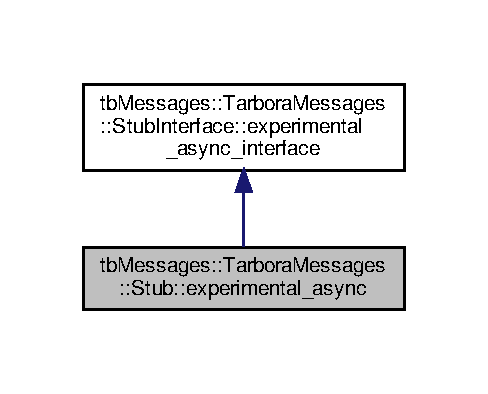
\includegraphics[width=234pt]{classtbMessages_1_1TarboraMessages_1_1Stub_1_1experimental__async__inherit__graph}
\end{center}
\end{figure}


Collaboration diagram for tb\+Messages\+:\+:Tarbora\+Messages\+:\+:Stub\+:\+:experimental\+\_\+async\+:
\nopagebreak
\begin{figure}[H]
\begin{center}
\leavevmode
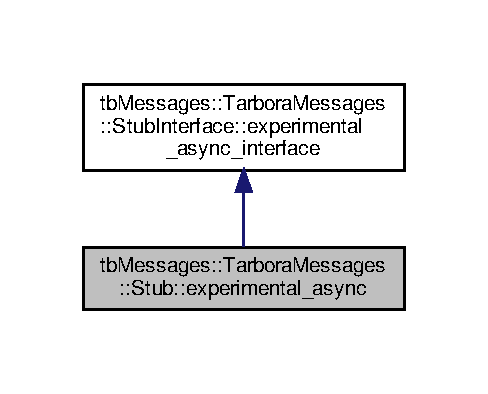
\includegraphics[width=234pt]{classtbMessages_1_1TarboraMessages_1_1Stub_1_1experimental__async__coll__graph}
\end{center}
\end{figure}
\subsection*{Public Member Functions}
\begin{DoxyCompactItemize}
\item 
\mbox{\Hypertarget{classtbMessages_1_1TarboraMessages_1_1Stub_1_1experimental__async_a855fc986d13856bd3d308070aa96e180}\label{classtbMessages_1_1TarboraMessages_1_1Stub_1_1experimental__async_a855fc986d13856bd3d308070aa96e180}} 
void {\bfseries Connect} (\+::grpc\+::\+Client\+Context $\ast$context, \+::grpc\+::experimental\+::\+Client\+Bidi\+Reactor$<$ \+::\hyperlink{classtbMessages_1_1Message}{tb\+Messages\+::\+Message},\+::\hyperlink{classtbMessages_1_1Message}{tb\+Messages\+::\+Message} $>$ $\ast$reactor) override
\item 
\mbox{\Hypertarget{classtbMessages_1_1TarboraMessages_1_1Stub_1_1experimental__async_a0ee0308563527ff0ad9c14c44584f4c2}\label{classtbMessages_1_1TarboraMessages_1_1Stub_1_1experimental__async_a0ee0308563527ff0ad9c14c44584f4c2}} 
void {\bfseries Subscribe} (\+::grpc\+::\+Client\+Context $\ast$context, const \+::\hyperlink{classtbMessages_1_1EventHeader}{tb\+Messages\+::\+Event\+Header} $\ast$request, \+::\hyperlink{classtbMessages_1_1Empty}{tb\+Messages\+::\+Empty} $\ast$response, std\+::function$<$ void(\+::grpc\+::\+Status)$>$) override
\item 
\mbox{\Hypertarget{classtbMessages_1_1TarboraMessages_1_1Stub_1_1experimental__async_a395c98899e693fa2edcaf8d8bbf56091}\label{classtbMessages_1_1TarboraMessages_1_1Stub_1_1experimental__async_a395c98899e693fa2edcaf8d8bbf56091}} 
void {\bfseries Subscribe} (\+::grpc\+::\+Client\+Context $\ast$context, const \+::grpc\+::\+Byte\+Buffer $\ast$request, \+::\hyperlink{classtbMessages_1_1Empty}{tb\+Messages\+::\+Empty} $\ast$response, std\+::function$<$ void(\+::grpc\+::\+Status)$>$) override
\item 
\mbox{\Hypertarget{classtbMessages_1_1TarboraMessages_1_1Stub_1_1experimental__async_a03ad7bb628e4904b6f4249bbde52a34e}\label{classtbMessages_1_1TarboraMessages_1_1Stub_1_1experimental__async_a03ad7bb628e4904b6f4249bbde52a34e}} 
void {\bfseries Subscribe} (\+::grpc\+::\+Client\+Context $\ast$context, const \+::\hyperlink{classtbMessages_1_1EventHeader}{tb\+Messages\+::\+Event\+Header} $\ast$request, \+::\hyperlink{classtbMessages_1_1Empty}{tb\+Messages\+::\+Empty} $\ast$response, \+::grpc\+::experimental\+::\+Client\+Unary\+Reactor $\ast$reactor) override
\item 
\mbox{\Hypertarget{classtbMessages_1_1TarboraMessages_1_1Stub_1_1experimental__async_ae41e1f79cd823d42c5591036a80d1247}\label{classtbMessages_1_1TarboraMessages_1_1Stub_1_1experimental__async_ae41e1f79cd823d42c5591036a80d1247}} 
void {\bfseries Subscribe} (\+::grpc\+::\+Client\+Context $\ast$context, const \+::grpc\+::\+Byte\+Buffer $\ast$request, \+::\hyperlink{classtbMessages_1_1Empty}{tb\+Messages\+::\+Empty} $\ast$response, \+::grpc\+::experimental\+::\+Client\+Unary\+Reactor $\ast$reactor) override
\item 
\mbox{\Hypertarget{classtbMessages_1_1TarboraMessages_1_1Stub_1_1experimental__async_a4d00a594930ea8597b99315a46b1d434}\label{classtbMessages_1_1TarboraMessages_1_1Stub_1_1experimental__async_a4d00a594930ea8597b99315a46b1d434}} 
void {\bfseries Desubscribe} (\+::grpc\+::\+Client\+Context $\ast$context, const \+::\hyperlink{classtbMessages_1_1EventHeader}{tb\+Messages\+::\+Event\+Header} $\ast$request, \+::\hyperlink{classtbMessages_1_1Empty}{tb\+Messages\+::\+Empty} $\ast$response, std\+::function$<$ void(\+::grpc\+::\+Status)$>$) override
\item 
\mbox{\Hypertarget{classtbMessages_1_1TarboraMessages_1_1Stub_1_1experimental__async_afd42a0d76f2b5bff9fccc0b5799d0504}\label{classtbMessages_1_1TarboraMessages_1_1Stub_1_1experimental__async_afd42a0d76f2b5bff9fccc0b5799d0504}} 
void {\bfseries Desubscribe} (\+::grpc\+::\+Client\+Context $\ast$context, const \+::grpc\+::\+Byte\+Buffer $\ast$request, \+::\hyperlink{classtbMessages_1_1Empty}{tb\+Messages\+::\+Empty} $\ast$response, std\+::function$<$ void(\+::grpc\+::\+Status)$>$) override
\item 
\mbox{\Hypertarget{classtbMessages_1_1TarboraMessages_1_1Stub_1_1experimental__async_a983db69de401f2316520c21b8cc48879}\label{classtbMessages_1_1TarboraMessages_1_1Stub_1_1experimental__async_a983db69de401f2316520c21b8cc48879}} 
void {\bfseries Desubscribe} (\+::grpc\+::\+Client\+Context $\ast$context, const \+::\hyperlink{classtbMessages_1_1EventHeader}{tb\+Messages\+::\+Event\+Header} $\ast$request, \+::\hyperlink{classtbMessages_1_1Empty}{tb\+Messages\+::\+Empty} $\ast$response, \+::grpc\+::experimental\+::\+Client\+Unary\+Reactor $\ast$reactor) override
\item 
\mbox{\Hypertarget{classtbMessages_1_1TarboraMessages_1_1Stub_1_1experimental__async_abe3f2922b9fc1ace6011342ae4d57dbd}\label{classtbMessages_1_1TarboraMessages_1_1Stub_1_1experimental__async_abe3f2922b9fc1ace6011342ae4d57dbd}} 
void {\bfseries Desubscribe} (\+::grpc\+::\+Client\+Context $\ast$context, const \+::grpc\+::\+Byte\+Buffer $\ast$request, \+::\hyperlink{classtbMessages_1_1Empty}{tb\+Messages\+::\+Empty} $\ast$response, \+::grpc\+::experimental\+::\+Client\+Unary\+Reactor $\ast$reactor) override
\end{DoxyCompactItemize}
\subsection*{Friends}
\begin{DoxyCompactItemize}
\item 
\mbox{\Hypertarget{classtbMessages_1_1TarboraMessages_1_1Stub_1_1experimental__async_a83cdea49df0bc777f54453927d691680}\label{classtbMessages_1_1TarboraMessages_1_1Stub_1_1experimental__async_a83cdea49df0bc777f54453927d691680}} 
class {\bfseries Stub}
\end{DoxyCompactItemize}


The documentation for this class was generated from the following files\+:\begin{DoxyCompactItemize}
\item 
Tarbora/\+Framework/\+Protos/messages.\+grpc.\+pb.\+h\item 
Tarbora/\+Framework/\+Protos/messages.\+grpc.\+pb.\+cc\end{DoxyCompactItemize}

\hypertarget{classtbMessages_1_1TarboraMessages_1_1StubInterface_1_1experimental__async__interface}{}\section{tb\+Messages\+:\+:Tarbora\+Messages\+:\+:Stub\+Interface\+:\+:experimental\+\_\+async\+\_\+interface Class Reference}
\label{classtbMessages_1_1TarboraMessages_1_1StubInterface_1_1experimental__async__interface}\index{tb\+Messages\+::\+Tarbora\+Messages\+::\+Stub\+Interface\+::experimental\+\_\+async\+\_\+interface@{tb\+Messages\+::\+Tarbora\+Messages\+::\+Stub\+Interface\+::experimental\+\_\+async\+\_\+interface}}


Inheritance diagram for tb\+Messages\+:\+:Tarbora\+Messages\+:\+:Stub\+Interface\+:\+:experimental\+\_\+async\+\_\+interface\+:
\nopagebreak
\begin{figure}[H]
\begin{center}
\leavevmode
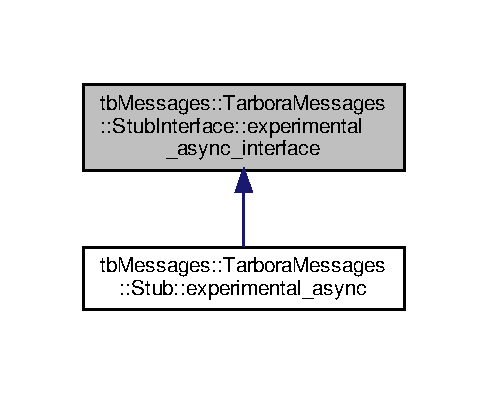
\includegraphics[width=234pt]{classtbMessages_1_1TarboraMessages_1_1StubInterface_1_1experimental__async__interface__inherit__graph}
\end{center}
\end{figure}
\subsection*{Public Member Functions}
\begin{DoxyCompactItemize}
\item 
\mbox{\Hypertarget{classtbMessages_1_1TarboraMessages_1_1StubInterface_1_1experimental__async__interface_a0238a497c5369e4b9c44d8bd73a2f807}\label{classtbMessages_1_1TarboraMessages_1_1StubInterface_1_1experimental__async__interface_a0238a497c5369e4b9c44d8bd73a2f807}} 
virtual void {\bfseries Connect} (\+::grpc\+::\+Client\+Context $\ast$context, \+::grpc\+::experimental\+::\+Client\+Bidi\+Reactor$<$ \+::\hyperlink{classtbMessages_1_1Message}{tb\+Messages\+::\+Message},\+::\hyperlink{classtbMessages_1_1Message}{tb\+Messages\+::\+Message} $>$ $\ast$reactor)=0
\item 
\mbox{\Hypertarget{classtbMessages_1_1TarboraMessages_1_1StubInterface_1_1experimental__async__interface_ac0c8863d1063081ee1f10cded0f70490}\label{classtbMessages_1_1TarboraMessages_1_1StubInterface_1_1experimental__async__interface_ac0c8863d1063081ee1f10cded0f70490}} 
virtual void {\bfseries Subscribe} (\+::grpc\+::\+Client\+Context $\ast$context, const \+::\hyperlink{classtbMessages_1_1EventHeader}{tb\+Messages\+::\+Event\+Header} $\ast$request, \+::\hyperlink{classtbMessages_1_1Empty}{tb\+Messages\+::\+Empty} $\ast$response, std\+::function$<$ void(\+::grpc\+::\+Status)$>$)=0
\item 
\mbox{\Hypertarget{classtbMessages_1_1TarboraMessages_1_1StubInterface_1_1experimental__async__interface_a1986fe54eda1e0a0c5a94f9cbcb865da}\label{classtbMessages_1_1TarboraMessages_1_1StubInterface_1_1experimental__async__interface_a1986fe54eda1e0a0c5a94f9cbcb865da}} 
virtual void {\bfseries Subscribe} (\+::grpc\+::\+Client\+Context $\ast$context, const \+::grpc\+::\+Byte\+Buffer $\ast$request, \+::\hyperlink{classtbMessages_1_1Empty}{tb\+Messages\+::\+Empty} $\ast$response, std\+::function$<$ void(\+::grpc\+::\+Status)$>$)=0
\item 
\mbox{\Hypertarget{classtbMessages_1_1TarboraMessages_1_1StubInterface_1_1experimental__async__interface_a392d730884aba5d51c4bc61c0e386b43}\label{classtbMessages_1_1TarboraMessages_1_1StubInterface_1_1experimental__async__interface_a392d730884aba5d51c4bc61c0e386b43}} 
virtual void {\bfseries Subscribe} (\+::grpc\+::\+Client\+Context $\ast$context, const \+::\hyperlink{classtbMessages_1_1EventHeader}{tb\+Messages\+::\+Event\+Header} $\ast$request, \+::\hyperlink{classtbMessages_1_1Empty}{tb\+Messages\+::\+Empty} $\ast$response, \+::grpc\+::experimental\+::\+Client\+Unary\+Reactor $\ast$reactor)=0
\item 
\mbox{\Hypertarget{classtbMessages_1_1TarboraMessages_1_1StubInterface_1_1experimental__async__interface_ad000e7f4af4d7bdc591fb12efe2a4f6a}\label{classtbMessages_1_1TarboraMessages_1_1StubInterface_1_1experimental__async__interface_ad000e7f4af4d7bdc591fb12efe2a4f6a}} 
virtual void {\bfseries Subscribe} (\+::grpc\+::\+Client\+Context $\ast$context, const \+::grpc\+::\+Byte\+Buffer $\ast$request, \+::\hyperlink{classtbMessages_1_1Empty}{tb\+Messages\+::\+Empty} $\ast$response, \+::grpc\+::experimental\+::\+Client\+Unary\+Reactor $\ast$reactor)=0
\item 
\mbox{\Hypertarget{classtbMessages_1_1TarboraMessages_1_1StubInterface_1_1experimental__async__interface_a65bd355f46f85a8ad505e8e1d9361596}\label{classtbMessages_1_1TarboraMessages_1_1StubInterface_1_1experimental__async__interface_a65bd355f46f85a8ad505e8e1d9361596}} 
virtual void {\bfseries Desubscribe} (\+::grpc\+::\+Client\+Context $\ast$context, const \+::\hyperlink{classtbMessages_1_1EventHeader}{tb\+Messages\+::\+Event\+Header} $\ast$request, \+::\hyperlink{classtbMessages_1_1Empty}{tb\+Messages\+::\+Empty} $\ast$response, std\+::function$<$ void(\+::grpc\+::\+Status)$>$)=0
\item 
\mbox{\Hypertarget{classtbMessages_1_1TarboraMessages_1_1StubInterface_1_1experimental__async__interface_a6063d57e55c61bdaf66959ebcba02ddc}\label{classtbMessages_1_1TarboraMessages_1_1StubInterface_1_1experimental__async__interface_a6063d57e55c61bdaf66959ebcba02ddc}} 
virtual void {\bfseries Desubscribe} (\+::grpc\+::\+Client\+Context $\ast$context, const \+::grpc\+::\+Byte\+Buffer $\ast$request, \+::\hyperlink{classtbMessages_1_1Empty}{tb\+Messages\+::\+Empty} $\ast$response, std\+::function$<$ void(\+::grpc\+::\+Status)$>$)=0
\item 
\mbox{\Hypertarget{classtbMessages_1_1TarboraMessages_1_1StubInterface_1_1experimental__async__interface_ad459837fd2285354f3713bb5ad647978}\label{classtbMessages_1_1TarboraMessages_1_1StubInterface_1_1experimental__async__interface_ad459837fd2285354f3713bb5ad647978}} 
virtual void {\bfseries Desubscribe} (\+::grpc\+::\+Client\+Context $\ast$context, const \+::\hyperlink{classtbMessages_1_1EventHeader}{tb\+Messages\+::\+Event\+Header} $\ast$request, \+::\hyperlink{classtbMessages_1_1Empty}{tb\+Messages\+::\+Empty} $\ast$response, \+::grpc\+::experimental\+::\+Client\+Unary\+Reactor $\ast$reactor)=0
\item 
\mbox{\Hypertarget{classtbMessages_1_1TarboraMessages_1_1StubInterface_1_1experimental__async__interface_a7c039addb9dad0c7302d81347bffc219}\label{classtbMessages_1_1TarboraMessages_1_1StubInterface_1_1experimental__async__interface_a7c039addb9dad0c7302d81347bffc219}} 
virtual void {\bfseries Desubscribe} (\+::grpc\+::\+Client\+Context $\ast$context, const \+::grpc\+::\+Byte\+Buffer $\ast$request, \+::\hyperlink{classtbMessages_1_1Empty}{tb\+Messages\+::\+Empty} $\ast$response, \+::grpc\+::experimental\+::\+Client\+Unary\+Reactor $\ast$reactor)=0
\end{DoxyCompactItemize}


The documentation for this class was generated from the following file\+:\begin{DoxyCompactItemize}
\item 
Tarbora/\+Framework/\+Protos/messages.\+grpc.\+pb.\+h\end{DoxyCompactItemize}

\hypertarget{classtbMessages_1_1TarboraMessages_1_1ExperimentalWithCallbackMethod__Connect}{}\section{tb\+Messages\+:\+:Tarbora\+Messages\+:\+:Experimental\+With\+Callback\+Method\+\_\+\+Connect$<$ Base\+Class $>$ Class Template Reference}
\label{classtbMessages_1_1TarboraMessages_1_1ExperimentalWithCallbackMethod__Connect}\index{tb\+Messages\+::\+Tarbora\+Messages\+::\+Experimental\+With\+Callback\+Method\+\_\+\+Connect$<$ Base\+Class $>$@{tb\+Messages\+::\+Tarbora\+Messages\+::\+Experimental\+With\+Callback\+Method\+\_\+\+Connect$<$ Base\+Class $>$}}


Inheritance diagram for tb\+Messages\+:\+:Tarbora\+Messages\+:\+:Experimental\+With\+Callback\+Method\+\_\+\+Connect$<$ Base\+Class $>$\+:
\nopagebreak
\begin{figure}[H]
\begin{center}
\leavevmode
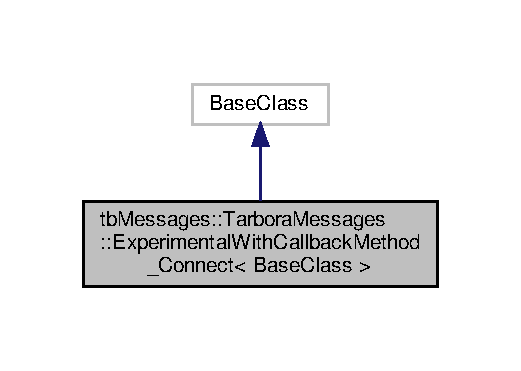
\includegraphics[width=250pt]{classtbMessages_1_1TarboraMessages_1_1ExperimentalWithCallbackMethod__Connect__inherit__graph}
\end{center}
\end{figure}


Collaboration diagram for tb\+Messages\+:\+:Tarbora\+Messages\+:\+:Experimental\+With\+Callback\+Method\+\_\+\+Connect$<$ Base\+Class $>$\+:
\nopagebreak
\begin{figure}[H]
\begin{center}
\leavevmode
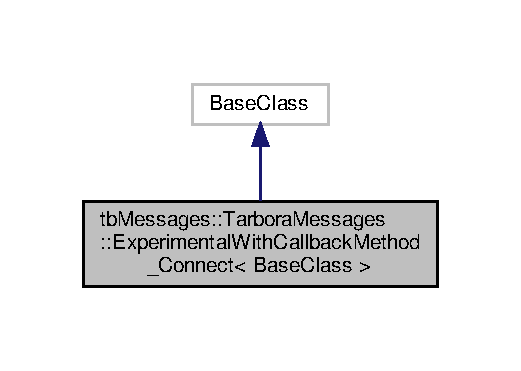
\includegraphics[width=250pt]{classtbMessages_1_1TarboraMessages_1_1ExperimentalWithCallbackMethod__Connect__coll__graph}
\end{center}
\end{figure}
\subsection*{Public Member Functions}
\begin{DoxyCompactItemize}
\item 
\mbox{\Hypertarget{classtbMessages_1_1TarboraMessages_1_1ExperimentalWithCallbackMethod__Connect_a0df1a2785b45e3ce8f86341203d1dae8}\label{classtbMessages_1_1TarboraMessages_1_1ExperimentalWithCallbackMethod__Connect_a0df1a2785b45e3ce8f86341203d1dae8}} 
\+::grpc\+::\+Status {\bfseries Connect} (\+::grpc\+::\+Server\+Context $\ast$context, \+::grpc\+::\+Server\+Reader\+Writer$<$ \+::\hyperlink{classtbMessages_1_1Message}{tb\+Messages\+::\+Message}, \+::\hyperlink{classtbMessages_1_1Message}{tb\+Messages\+::\+Message} $>$ $\ast$stream) override
\item 
\mbox{\Hypertarget{classtbMessages_1_1TarboraMessages_1_1ExperimentalWithCallbackMethod__Connect_a5e887f897381c082962770541db3d397}\label{classtbMessages_1_1TarboraMessages_1_1ExperimentalWithCallbackMethod__Connect_a5e887f897381c082962770541db3d397}} 
virtual \+::grpc\+::experimental\+::\+Server\+Bidi\+Reactor$<$ \+::\hyperlink{classtbMessages_1_1Message}{tb\+Messages\+::\+Message}, \+::\hyperlink{classtbMessages_1_1Message}{tb\+Messages\+::\+Message} $>$ $\ast$ {\bfseries Connect} ()
\end{DoxyCompactItemize}


The documentation for this class was generated from the following file\+:\begin{DoxyCompactItemize}
\item 
Tarbora/\+Framework/\+Protos/messages.\+grpc.\+pb.\+h\end{DoxyCompactItemize}

\hypertarget{classtbMessages_1_1TarboraMessages_1_1ExperimentalWithCallbackMethod__Desubscribe}{}\section{tb\+Messages\+:\+:Tarbora\+Messages\+:\+:Experimental\+With\+Callback\+Method\+\_\+\+Desubscribe$<$ Base\+Class $>$ Class Template Reference}
\label{classtbMessages_1_1TarboraMessages_1_1ExperimentalWithCallbackMethod__Desubscribe}\index{tb\+Messages\+::\+Tarbora\+Messages\+::\+Experimental\+With\+Callback\+Method\+\_\+\+Desubscribe$<$ Base\+Class $>$@{tb\+Messages\+::\+Tarbora\+Messages\+::\+Experimental\+With\+Callback\+Method\+\_\+\+Desubscribe$<$ Base\+Class $>$}}


Inheritance diagram for tb\+Messages\+:\+:Tarbora\+Messages\+:\+:Experimental\+With\+Callback\+Method\+\_\+\+Desubscribe$<$ Base\+Class $>$\+:
\nopagebreak
\begin{figure}[H]
\begin{center}
\leavevmode
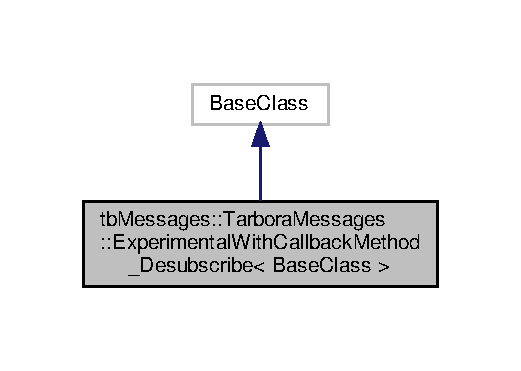
\includegraphics[width=250pt]{classtbMessages_1_1TarboraMessages_1_1ExperimentalWithCallbackMethod__Desubscribe__inherit__graph}
\end{center}
\end{figure}


Collaboration diagram for tb\+Messages\+:\+:Tarbora\+Messages\+:\+:Experimental\+With\+Callback\+Method\+\_\+\+Desubscribe$<$ Base\+Class $>$\+:
\nopagebreak
\begin{figure}[H]
\begin{center}
\leavevmode
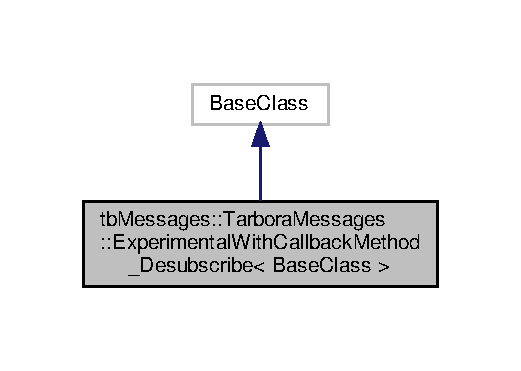
\includegraphics[width=250pt]{classtbMessages_1_1TarboraMessages_1_1ExperimentalWithCallbackMethod__Desubscribe__coll__graph}
\end{center}
\end{figure}
\subsection*{Public Member Functions}
\begin{DoxyCompactItemize}
\item 
\mbox{\Hypertarget{classtbMessages_1_1TarboraMessages_1_1ExperimentalWithCallbackMethod__Desubscribe_ad059a36f9d33f1be11be0df69f0e6d2c}\label{classtbMessages_1_1TarboraMessages_1_1ExperimentalWithCallbackMethod__Desubscribe_ad059a36f9d33f1be11be0df69f0e6d2c}} 
void {\bfseries Set\+Message\+Allocator\+For\+\_\+\+Desubscribe} (\+::\hyperlink{classgrpc_1_1experimental_1_1MessageAllocator}{grpc\+::experimental\+::\+Message\+Allocator}$<$ \+::\hyperlink{classtbMessages_1_1EventHeader}{tb\+Messages\+::\+Event\+Header}, \+::\hyperlink{classtbMessages_1_1Empty}{tb\+Messages\+::\+Empty} $>$ $\ast$allocator)
\item 
\mbox{\Hypertarget{classtbMessages_1_1TarboraMessages_1_1ExperimentalWithCallbackMethod__Desubscribe_a9d1bbd7b9de681b64c7e997b68dcfe46}\label{classtbMessages_1_1TarboraMessages_1_1ExperimentalWithCallbackMethod__Desubscribe_a9d1bbd7b9de681b64c7e997b68dcfe46}} 
\+::grpc\+::\+Status {\bfseries Desubscribe} (\+::grpc\+::\+Server\+Context $\ast$context, const \+::\hyperlink{classtbMessages_1_1EventHeader}{tb\+Messages\+::\+Event\+Header} $\ast$request, \+::\hyperlink{classtbMessages_1_1Empty}{tb\+Messages\+::\+Empty} $\ast$response) override
\item 
\mbox{\Hypertarget{classtbMessages_1_1TarboraMessages_1_1ExperimentalWithCallbackMethod__Desubscribe_abbcf53fac3facf9bc424c716a2f3d9d7}\label{classtbMessages_1_1TarboraMessages_1_1ExperimentalWithCallbackMethod__Desubscribe_abbcf53fac3facf9bc424c716a2f3d9d7}} 
virtual void {\bfseries Desubscribe} (\+::grpc\+::\+Server\+Context $\ast$context, const \+::\hyperlink{classtbMessages_1_1EventHeader}{tb\+Messages\+::\+Event\+Header} $\ast$request, \+::\hyperlink{classtbMessages_1_1Empty}{tb\+Messages\+::\+Empty} $\ast$response, \+::grpc\+::experimental\+::\+Server\+Callback\+Rpc\+Controller $\ast$controller)
\end{DoxyCompactItemize}


The documentation for this class was generated from the following file\+:\begin{DoxyCompactItemize}
\item 
Tarbora/\+Framework/\+Protos/messages.\+grpc.\+pb.\+h\end{DoxyCompactItemize}

\hypertarget{classtbMessages_1_1TarboraMessages_1_1ExperimentalWithCallbackMethod__Subscribe}{}\section{tb\+Messages\+:\+:Tarbora\+Messages\+:\+:Experimental\+With\+Callback\+Method\+\_\+\+Subscribe$<$ Base\+Class $>$ Class Template Reference}
\label{classtbMessages_1_1TarboraMessages_1_1ExperimentalWithCallbackMethod__Subscribe}\index{tb\+Messages\+::\+Tarbora\+Messages\+::\+Experimental\+With\+Callback\+Method\+\_\+\+Subscribe$<$ Base\+Class $>$@{tb\+Messages\+::\+Tarbora\+Messages\+::\+Experimental\+With\+Callback\+Method\+\_\+\+Subscribe$<$ Base\+Class $>$}}


Inheritance diagram for tb\+Messages\+:\+:Tarbora\+Messages\+:\+:Experimental\+With\+Callback\+Method\+\_\+\+Subscribe$<$ Base\+Class $>$\+:
\nopagebreak
\begin{figure}[H]
\begin{center}
\leavevmode
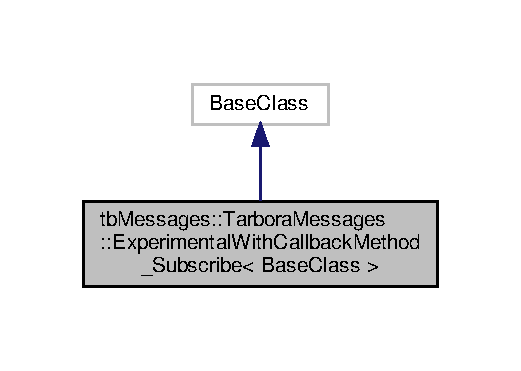
\includegraphics[width=250pt]{classtbMessages_1_1TarboraMessages_1_1ExperimentalWithCallbackMethod__Subscribe__inherit__graph}
\end{center}
\end{figure}


Collaboration diagram for tb\+Messages\+:\+:Tarbora\+Messages\+:\+:Experimental\+With\+Callback\+Method\+\_\+\+Subscribe$<$ Base\+Class $>$\+:
\nopagebreak
\begin{figure}[H]
\begin{center}
\leavevmode
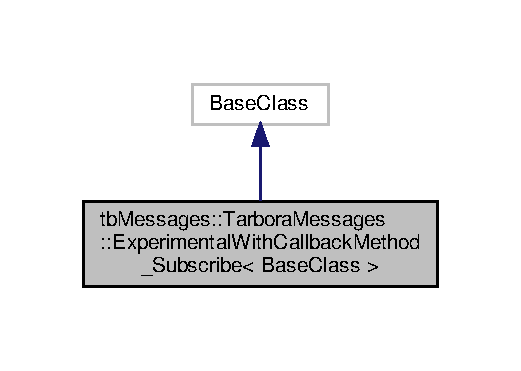
\includegraphics[width=250pt]{classtbMessages_1_1TarboraMessages_1_1ExperimentalWithCallbackMethod__Subscribe__coll__graph}
\end{center}
\end{figure}
\subsection*{Public Member Functions}
\begin{DoxyCompactItemize}
\item 
\mbox{\Hypertarget{classtbMessages_1_1TarboraMessages_1_1ExperimentalWithCallbackMethod__Subscribe_a55441070d9aaeb952650c61e71cfaf41}\label{classtbMessages_1_1TarboraMessages_1_1ExperimentalWithCallbackMethod__Subscribe_a55441070d9aaeb952650c61e71cfaf41}} 
void {\bfseries Set\+Message\+Allocator\+For\+\_\+\+Subscribe} (\+::\hyperlink{classgrpc_1_1experimental_1_1MessageAllocator}{grpc\+::experimental\+::\+Message\+Allocator}$<$ \+::\hyperlink{classtbMessages_1_1EventHeader}{tb\+Messages\+::\+Event\+Header}, \+::\hyperlink{classtbMessages_1_1Empty}{tb\+Messages\+::\+Empty} $>$ $\ast$allocator)
\item 
\mbox{\Hypertarget{classtbMessages_1_1TarboraMessages_1_1ExperimentalWithCallbackMethod__Subscribe_a7a764dfac6086ebc152145fb790e6cdb}\label{classtbMessages_1_1TarboraMessages_1_1ExperimentalWithCallbackMethod__Subscribe_a7a764dfac6086ebc152145fb790e6cdb}} 
\+::grpc\+::\+Status {\bfseries Subscribe} (\+::grpc\+::\+Server\+Context $\ast$context, const \+::\hyperlink{classtbMessages_1_1EventHeader}{tb\+Messages\+::\+Event\+Header} $\ast$request, \+::\hyperlink{classtbMessages_1_1Empty}{tb\+Messages\+::\+Empty} $\ast$response) override
\item 
\mbox{\Hypertarget{classtbMessages_1_1TarboraMessages_1_1ExperimentalWithCallbackMethod__Subscribe_a86d51001bd5a50bd2312613980994617}\label{classtbMessages_1_1TarboraMessages_1_1ExperimentalWithCallbackMethod__Subscribe_a86d51001bd5a50bd2312613980994617}} 
virtual void {\bfseries Subscribe} (\+::grpc\+::\+Server\+Context $\ast$context, const \+::\hyperlink{classtbMessages_1_1EventHeader}{tb\+Messages\+::\+Event\+Header} $\ast$request, \+::\hyperlink{classtbMessages_1_1Empty}{tb\+Messages\+::\+Empty} $\ast$response, \+::grpc\+::experimental\+::\+Server\+Callback\+Rpc\+Controller $\ast$controller)
\end{DoxyCompactItemize}


The documentation for this class was generated from the following file\+:\begin{DoxyCompactItemize}
\item 
Tarbora/\+Framework/\+Protos/messages.\+grpc.\+pb.\+h\end{DoxyCompactItemize}

\hypertarget{classtbMessages_1_1TarboraMessages_1_1ExperimentalWithRawCallbackMethod__Connect}{}\section{tb\+Messages\+:\+:Tarbora\+Messages\+:\+:Experimental\+With\+Raw\+Callback\+Method\+\_\+\+Connect$<$ Base\+Class $>$ Class Template Reference}
\label{classtbMessages_1_1TarboraMessages_1_1ExperimentalWithRawCallbackMethod__Connect}\index{tb\+Messages\+::\+Tarbora\+Messages\+::\+Experimental\+With\+Raw\+Callback\+Method\+\_\+\+Connect$<$ Base\+Class $>$@{tb\+Messages\+::\+Tarbora\+Messages\+::\+Experimental\+With\+Raw\+Callback\+Method\+\_\+\+Connect$<$ Base\+Class $>$}}


Inheritance diagram for tb\+Messages\+:\+:Tarbora\+Messages\+:\+:Experimental\+With\+Raw\+Callback\+Method\+\_\+\+Connect$<$ Base\+Class $>$\+:
\nopagebreak
\begin{figure}[H]
\begin{center}
\leavevmode
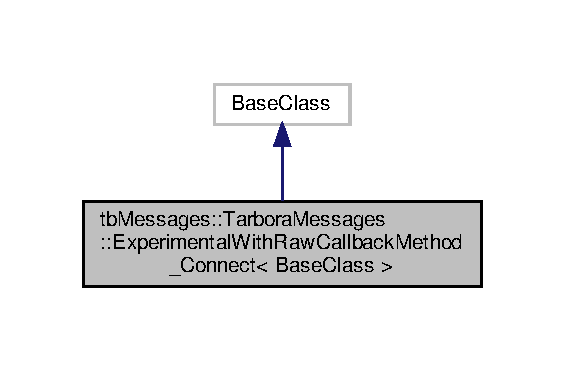
\includegraphics[width=271pt]{classtbMessages_1_1TarboraMessages_1_1ExperimentalWithRawCallbackMethod__Connect__inherit__graph}
\end{center}
\end{figure}


Collaboration diagram for tb\+Messages\+:\+:Tarbora\+Messages\+:\+:Experimental\+With\+Raw\+Callback\+Method\+\_\+\+Connect$<$ Base\+Class $>$\+:
\nopagebreak
\begin{figure}[H]
\begin{center}
\leavevmode
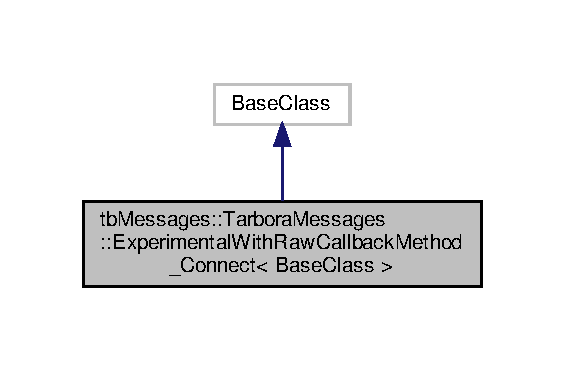
\includegraphics[width=271pt]{classtbMessages_1_1TarboraMessages_1_1ExperimentalWithRawCallbackMethod__Connect__coll__graph}
\end{center}
\end{figure}
\subsection*{Public Member Functions}
\begin{DoxyCompactItemize}
\item 
\mbox{\Hypertarget{classtbMessages_1_1TarboraMessages_1_1ExperimentalWithRawCallbackMethod__Connect_ae03e894dd39651f082655c93c6abcd13}\label{classtbMessages_1_1TarboraMessages_1_1ExperimentalWithRawCallbackMethod__Connect_ae03e894dd39651f082655c93c6abcd13}} 
\+::grpc\+::\+Status {\bfseries Connect} (\+::grpc\+::\+Server\+Context $\ast$context, \+::grpc\+::\+Server\+Reader\+Writer$<$ \+::\hyperlink{classtbMessages_1_1Message}{tb\+Messages\+::\+Message}, \+::\hyperlink{classtbMessages_1_1Message}{tb\+Messages\+::\+Message} $>$ $\ast$stream) override
\item 
\mbox{\Hypertarget{classtbMessages_1_1TarboraMessages_1_1ExperimentalWithRawCallbackMethod__Connect_a60596e519a519e9c9904434b22a9e0c5}\label{classtbMessages_1_1TarboraMessages_1_1ExperimentalWithRawCallbackMethod__Connect_a60596e519a519e9c9904434b22a9e0c5}} 
virtual \+::grpc\+::experimental\+::\+Server\+Bidi\+Reactor$<$ \+::grpc\+::\+Byte\+Buffer, \+::grpc\+::\+Byte\+Buffer $>$ $\ast$ {\bfseries Connect} ()
\end{DoxyCompactItemize}


The documentation for this class was generated from the following file\+:\begin{DoxyCompactItemize}
\item 
Tarbora/\+Framework/\+Protos/messages.\+grpc.\+pb.\+h\end{DoxyCompactItemize}

\hypertarget{classtbMessages_1_1TarboraMessages_1_1ExperimentalWithRawCallbackMethod__Desubscribe}{}\section{tb\+Messages\+:\+:Tarbora\+Messages\+:\+:Experimental\+With\+Raw\+Callback\+Method\+\_\+\+Desubscribe$<$ Base\+Class $>$ Class Template Reference}
\label{classtbMessages_1_1TarboraMessages_1_1ExperimentalWithRawCallbackMethod__Desubscribe}\index{tb\+Messages\+::\+Tarbora\+Messages\+::\+Experimental\+With\+Raw\+Callback\+Method\+\_\+\+Desubscribe$<$ Base\+Class $>$@{tb\+Messages\+::\+Tarbora\+Messages\+::\+Experimental\+With\+Raw\+Callback\+Method\+\_\+\+Desubscribe$<$ Base\+Class $>$}}


Inheritance diagram for tb\+Messages\+:\+:Tarbora\+Messages\+:\+:Experimental\+With\+Raw\+Callback\+Method\+\_\+\+Desubscribe$<$ Base\+Class $>$\+:
\nopagebreak
\begin{figure}[H]
\begin{center}
\leavevmode
\includegraphics[width=271pt]{classtbMessages_1_1TarboraMessages_1_1ExperimentalWithRawCallbackMethod__Desubscribe__inherit__graph}
\end{center}
\end{figure}


Collaboration diagram for tb\+Messages\+:\+:Tarbora\+Messages\+:\+:Experimental\+With\+Raw\+Callback\+Method\+\_\+\+Desubscribe$<$ Base\+Class $>$\+:
\nopagebreak
\begin{figure}[H]
\begin{center}
\leavevmode
\includegraphics[width=271pt]{classtbMessages_1_1TarboraMessages_1_1ExperimentalWithRawCallbackMethod__Desubscribe__coll__graph}
\end{center}
\end{figure}
\subsection*{Public Member Functions}
\begin{DoxyCompactItemize}
\item 
\mbox{\Hypertarget{classtbMessages_1_1TarboraMessages_1_1ExperimentalWithRawCallbackMethod__Desubscribe_a5e5d7bf517952185b6ad763b8a1645f6}\label{classtbMessages_1_1TarboraMessages_1_1ExperimentalWithRawCallbackMethod__Desubscribe_a5e5d7bf517952185b6ad763b8a1645f6}} 
\+::grpc\+::\+Status {\bfseries Desubscribe} (\+::grpc\+::\+Server\+Context $\ast$context, const \+::\hyperlink{classtbMessages_1_1EventHeader}{tb\+Messages\+::\+Event\+Header} $\ast$request, \+::\hyperlink{classtbMessages_1_1Empty}{tb\+Messages\+::\+Empty} $\ast$response) override
\item 
\mbox{\Hypertarget{classtbMessages_1_1TarboraMessages_1_1ExperimentalWithRawCallbackMethod__Desubscribe_acdd9b596c3c87ec85b19981bad38080b}\label{classtbMessages_1_1TarboraMessages_1_1ExperimentalWithRawCallbackMethod__Desubscribe_acdd9b596c3c87ec85b19981bad38080b}} 
virtual void {\bfseries Desubscribe} (\+::grpc\+::\+Server\+Context $\ast$context, const \+::grpc\+::\+Byte\+Buffer $\ast$request, \+::grpc\+::\+Byte\+Buffer $\ast$response, \+::grpc\+::experimental\+::\+Server\+Callback\+Rpc\+Controller $\ast$controller)
\end{DoxyCompactItemize}


The documentation for this class was generated from the following file\+:\begin{DoxyCompactItemize}
\item 
Tarbora/\+Framework/\+Protos/messages.\+grpc.\+pb.\+h\end{DoxyCompactItemize}

\hypertarget{classtbMessages_1_1TarboraMessages_1_1ExperimentalWithRawCallbackMethod__Subscribe}{}\section{tb\+Messages\+:\+:Tarbora\+Messages\+:\+:Experimental\+With\+Raw\+Callback\+Method\+\_\+\+Subscribe$<$ Base\+Class $>$ Class Template Reference}
\label{classtbMessages_1_1TarboraMessages_1_1ExperimentalWithRawCallbackMethod__Subscribe}\index{tb\+Messages\+::\+Tarbora\+Messages\+::\+Experimental\+With\+Raw\+Callback\+Method\+\_\+\+Subscribe$<$ Base\+Class $>$@{tb\+Messages\+::\+Tarbora\+Messages\+::\+Experimental\+With\+Raw\+Callback\+Method\+\_\+\+Subscribe$<$ Base\+Class $>$}}


Inheritance diagram for tb\+Messages\+:\+:Tarbora\+Messages\+:\+:Experimental\+With\+Raw\+Callback\+Method\+\_\+\+Subscribe$<$ Base\+Class $>$\+:
\nopagebreak
\begin{figure}[H]
\begin{center}
\leavevmode
\includegraphics[width=271pt]{classtbMessages_1_1TarboraMessages_1_1ExperimentalWithRawCallbackMethod__Subscribe__inherit__graph}
\end{center}
\end{figure}


Collaboration diagram for tb\+Messages\+:\+:Tarbora\+Messages\+:\+:Experimental\+With\+Raw\+Callback\+Method\+\_\+\+Subscribe$<$ Base\+Class $>$\+:
\nopagebreak
\begin{figure}[H]
\begin{center}
\leavevmode
\includegraphics[width=271pt]{classtbMessages_1_1TarboraMessages_1_1ExperimentalWithRawCallbackMethod__Subscribe__coll__graph}
\end{center}
\end{figure}
\subsection*{Public Member Functions}
\begin{DoxyCompactItemize}
\item 
\mbox{\Hypertarget{classtbMessages_1_1TarboraMessages_1_1ExperimentalWithRawCallbackMethod__Subscribe_ab8d988e5c17710b32c695667e9fba129}\label{classtbMessages_1_1TarboraMessages_1_1ExperimentalWithRawCallbackMethod__Subscribe_ab8d988e5c17710b32c695667e9fba129}} 
\+::grpc\+::\+Status {\bfseries Subscribe} (\+::grpc\+::\+Server\+Context $\ast$context, const \+::\hyperlink{classtbMessages_1_1EventHeader}{tb\+Messages\+::\+Event\+Header} $\ast$request, \+::\hyperlink{classtbMessages_1_1Empty}{tb\+Messages\+::\+Empty} $\ast$response) override
\item 
\mbox{\Hypertarget{classtbMessages_1_1TarboraMessages_1_1ExperimentalWithRawCallbackMethod__Subscribe_a78d3f1b368c22b71e60ef9f6daae9411}\label{classtbMessages_1_1TarboraMessages_1_1ExperimentalWithRawCallbackMethod__Subscribe_a78d3f1b368c22b71e60ef9f6daae9411}} 
virtual void {\bfseries Subscribe} (\+::grpc\+::\+Server\+Context $\ast$context, const \+::grpc\+::\+Byte\+Buffer $\ast$request, \+::grpc\+::\+Byte\+Buffer $\ast$response, \+::grpc\+::experimental\+::\+Server\+Callback\+Rpc\+Controller $\ast$controller)
\end{DoxyCompactItemize}


The documentation for this class was generated from the following file\+:\begin{DoxyCompactItemize}
\item 
Tarbora/\+Framework/\+Protos/messages.\+grpc.\+pb.\+h\end{DoxyCompactItemize}

\hypertarget{classTarbora_1_1GameLayerImpl}{}\section{Tarbora\+:\+:Game\+Layer\+Impl Class Reference}
\label{classTarbora_1_1GameLayerImpl}\index{Tarbora\+::\+Game\+Layer\+Impl@{Tarbora\+::\+Game\+Layer\+Impl}}


Inheritance diagram for Tarbora\+:\+:Game\+Layer\+Impl\+:
\nopagebreak
\begin{figure}[H]
\begin{center}
\leavevmode
\includegraphics[width=217pt]{classTarbora_1_1GameLayerImpl__inherit__graph}
\end{center}
\end{figure}


Collaboration diagram for Tarbora\+:\+:Game\+Layer\+Impl\+:
\nopagebreak
\begin{figure}[H]
\begin{center}
\leavevmode
\includegraphics[width=217pt]{classTarbora_1_1GameLayerImpl__coll__graph}
\end{center}
\end{figure}
\subsection*{Public Member Functions}
\begin{DoxyCompactItemize}
\item 
\mbox{\Hypertarget{classTarbora_1_1GameLayerImpl_ae96df1359f37e2850008dde83a348f7f}\label{classTarbora_1_1GameLayerImpl_ae96df1359f37e2850008dde83a348f7f}} 
{\bfseries Game\+Layer\+Impl} (\hyperlink{classTarbora_1_1GraphicView}{Graphic\+View} $\ast$view, bool start\+\_\+active=true)
\item 
\mbox{\Hypertarget{classTarbora_1_1GameLayerImpl_aaa12f4d9e7d3cea6a2095b76248fac83}\label{classTarbora_1_1GameLayerImpl_aaa12f4d9e7d3cea6a2095b76248fac83}} 
virtual bool {\bfseries On\+Message} (\hyperlink{classTarbora_1_1MessageBody}{Message\+Body} $\ast$m) override
\item 
\mbox{\Hypertarget{classTarbora_1_1GameLayerImpl_a2ca17d3af2ffbdd4bdf3a6f1fbd0b62d}\label{classTarbora_1_1GameLayerImpl_a2ca17d3af2ffbdd4bdf3a6f1fbd0b62d}} 
virtual void {\bfseries Get\+Input} () override
\item 
\mbox{\Hypertarget{classTarbora_1_1GameLayerImpl_a1cf535da3b752490b5de5bd2df719942}\label{classTarbora_1_1GameLayerImpl_a1cf535da3b752490b5de5bd2df719942}} 
virtual void {\bfseries Update} (float delta\+Time) override
\item 
\mbox{\Hypertarget{classTarbora_1_1GameLayerImpl_a818b88ba9853bd72b1a11fc9f1df2b2d}\label{classTarbora_1_1GameLayerImpl_a818b88ba9853bd72b1a11fc9f1df2b2d}} 
virtual void {\bfseries Draw} () override
\item 
\mbox{\Hypertarget{classTarbora_1_1GameLayerImpl_a0f3e332d0e0a237cb51de7fe5935a2cd}\label{classTarbora_1_1GameLayerImpl_a0f3e332d0e0a237cb51de7fe5935a2cd}} 
void {\bfseries Set\+Target\+Id} (Actor\+Id id)
\item 
\mbox{\Hypertarget{classTarbora_1_1GameLayerImpl_ade4c1f74eca8d20d870cdd2b4d61361f}\label{classTarbora_1_1GameLayerImpl_ade4c1f74eca8d20d870cdd2b4d61361f}} 
Actor\+Id {\bfseries Get\+Target\+Id} () const
\end{DoxyCompactItemize}
\subsection*{Additional Inherited Members}


The documentation for this class was generated from the following files\+:\begin{DoxyCompactItemize}
\item 
Tarbora/\+Views/\+Graphic\+Views/inc/Game\+Layer.\+hpp\item 
Tarbora/\+Views/\+Graphic\+Views/src/Game\+Layer.\+cpp\end{DoxyCompactItemize}

\hypertarget{classTarbora_1_1GraphicsEngineImpl}{}\section{Tarbora\+:\+:Graphics\+Engine\+Impl Class Reference}
\label{classTarbora_1_1GraphicsEngineImpl}\index{Tarbora\+::\+Graphics\+Engine\+Impl@{Tarbora\+::\+Graphics\+Engine\+Impl}}
\subsection*{Public Member Functions}
\begin{DoxyCompactItemize}
\item 
\mbox{\Hypertarget{classTarbora_1_1GraphicsEngineImpl_a1290f63105d954932fad98302dd735a1}\label{classTarbora_1_1GraphicsEngineImpl_a1290f63105d954932fad98302dd735a1}} 
{\bfseries Graphics\+Engine\+Impl} (\hyperlink{classTarbora_1_1GraphicView}{Graphic\+View} $\ast$view, std\+::string settings\+\_\+file)
\item 
\mbox{\Hypertarget{classTarbora_1_1GraphicsEngineImpl_a271bcc842a745977dc5c107bdef17593}\label{classTarbora_1_1GraphicsEngineImpl_a271bcc842a745977dc5c107bdef17593}} 
void {\bfseries Init\+Gui} ()
\item 
\mbox{\Hypertarget{classTarbora_1_1GraphicsEngineImpl_ae3baad87b312efa383edf23cbe5b0381}\label{classTarbora_1_1GraphicsEngineImpl_ae3baad87b312efa383edf23cbe5b0381}} 
void {\bfseries Before\+Draw} ()
\item 
\mbox{\Hypertarget{classTarbora_1_1GraphicsEngineImpl_a2e4a1d8864d2a63dea5987d54b01ba83}\label{classTarbora_1_1GraphicsEngineImpl_a2e4a1d8864d2a63dea5987d54b01ba83}} 
void {\bfseries Draw\+Mesh} (std\+::shared\+\_\+ptr$<$ \hyperlink{classTarbora_1_1Mesh}{Mesh} $>$ mesh)
\item 
\mbox{\Hypertarget{classTarbora_1_1GraphicsEngineImpl_a5b3a5229c8614accf57072cb4f949006}\label{classTarbora_1_1GraphicsEngineImpl_a5b3a5229c8614accf57072cb4f949006}} 
void {\bfseries After\+Draw} ()
\item 
\mbox{\Hypertarget{classTarbora_1_1GraphicsEngineImpl_a8445c731da2c2ab7b0807be26d35d01b}\label{classTarbora_1_1GraphicsEngineImpl_a8445c731da2c2ab7b0807be26d35d01b}} 
void {\bfseries Before\+Draw\+Sky} ()
\item 
\mbox{\Hypertarget{classTarbora_1_1GraphicsEngineImpl_abd928d13f96ce114553411d55715d4d6}\label{classTarbora_1_1GraphicsEngineImpl_abd928d13f96ce114553411d55715d4d6}} 
void {\bfseries After\+Draw\+Sky} ()
\item 
\mbox{\Hypertarget{classTarbora_1_1GraphicsEngineImpl_a44ad31f6303619f33315b496c86c1dc6}\label{classTarbora_1_1GraphicsEngineImpl_a44ad31f6303619f33315b496c86c1dc6}} 
Window\+Ptr {\bfseries Get\+Window} ()
\item 
\mbox{\Hypertarget{classTarbora_1_1GraphicsEngineImpl_ae6c57654e7de209fd96b461cd317e31e}\label{classTarbora_1_1GraphicsEngineImpl_ae6c57654e7de209fd96b461cd317e31e}} 
unsigned int {\bfseries Compile\+Shader} (std\+::string type, const char $\ast$code)
\item 
\mbox{\Hypertarget{classTarbora_1_1GraphicsEngineImpl_ae62c4a4806ee3a0ed6de7603f032a5ab}\label{classTarbora_1_1GraphicsEngineImpl_ae62c4a4806ee3a0ed6de7603f032a5ab}} 
unsigned int {\bfseries Link\+Program} (unsigned int $\ast$ids)
\item 
\mbox{\Hypertarget{classTarbora_1_1GraphicsEngineImpl_a5cf62fc17bac7b40d285e4a71c3d8448}\label{classTarbora_1_1GraphicsEngineImpl_a5cf62fc17bac7b40d285e4a71c3d8448}} 
void {\bfseries Delete\+Program} (unsigned int id)
\item 
\mbox{\Hypertarget{classTarbora_1_1GraphicsEngineImpl_a89d8e735303e33f3e2f8d3610f496b6d}\label{classTarbora_1_1GraphicsEngineImpl_a89d8e735303e33f3e2f8d3610f496b6d}} 
unsigned int {\bfseries Load\+Texture} (unsigned char $\ast$data, int width, int height, int nr\+Components)
\item 
\mbox{\Hypertarget{classTarbora_1_1GraphicsEngineImpl_a4185bcc1646d432d5d1bb645c7e9a6f9}\label{classTarbora_1_1GraphicsEngineImpl_a4185bcc1646d432d5d1bb645c7e9a6f9}} 
void {\bfseries Bind\+Texture} (unsigned int id)
\item 
\mbox{\Hypertarget{classTarbora_1_1GraphicsEngineImpl_a4d50be41a34070713de06cf55ad3a18c}\label{classTarbora_1_1GraphicsEngineImpl_a4d50be41a34070713de06cf55ad3a18c}} 
void {\bfseries Delete\+Texture} (unsigned int id)
\item 
\mbox{\Hypertarget{classTarbora_1_1GraphicsEngineImpl_a66b0a4dcfe39cdda4b6ac5e7319804e7}\label{classTarbora_1_1GraphicsEngineImpl_a66b0a4dcfe39cdda4b6ac5e7319804e7}} 
unsigned int {\bfseries Load\+Mesh} (std\+::vector$<$ float $>$ vertices)
\item 
\mbox{\Hypertarget{classTarbora_1_1GraphicsEngineImpl_aade9c84e588f0fb651db238ae640eaae}\label{classTarbora_1_1GraphicsEngineImpl_aade9c84e588f0fb651db238ae640eaae}} 
void {\bfseries Delete\+Mesh} (unsigned int id)
\item 
\mbox{\Hypertarget{classTarbora_1_1GraphicsEngineImpl_ac710eacee5c718cc3655b2d393163ad4}\label{classTarbora_1_1GraphicsEngineImpl_ac710eacee5c718cc3655b2d393163ad4}} 
void {\bfseries Use\+Shader} (std\+::shared\+\_\+ptr$<$ \hyperlink{classTarbora_1_1Shader}{Shader} $>$ shader)
\item 
\mbox{\Hypertarget{classTarbora_1_1GraphicsEngineImpl_a58d55fc50cc0ee4441826bea5027becd}\label{classTarbora_1_1GraphicsEngineImpl_a58d55fc50cc0ee4441826bea5027becd}} 
std\+::shared\+\_\+ptr$<$ \hyperlink{classTarbora_1_1Shader}{Shader} $>$ {\bfseries Get\+Shader} ()
\item 
\mbox{\Hypertarget{classTarbora_1_1GraphicsEngineImpl_a0ac12dc1b663d4f5ae5bde9e4b27989f}\label{classTarbora_1_1GraphicsEngineImpl_a0ac12dc1b663d4f5ae5bde9e4b27989f}} 
bool {\bfseries Shader\+Available} ()
\item 
\mbox{\Hypertarget{classTarbora_1_1GraphicsEngineImpl_a07411627d0080e64e107a4259b82d970}\label{classTarbora_1_1GraphicsEngineImpl_a07411627d0080e64e107a4259b82d970}} 
int {\bfseries Take\+Screenshot} (const std\+::string \&filename)
\end{DoxyCompactItemize}


The documentation for this class was generated from the following files\+:\begin{DoxyCompactItemize}
\item 
Tarbora/\+Views/\+Graphics\+Engine/inc/Graphics\+Engine.\+hpp\item 
Tarbora/\+Views/\+Graphics\+Engine/src/Graphics\+Engine.\+cpp\end{DoxyCompactItemize}

\hypertarget{classTarbora_1_1GraphicView}{}\section{Tarbora\+:\+:Graphic\+View Class Reference}
\label{classTarbora_1_1GraphicView}\index{Tarbora\+::\+Graphic\+View@{Tarbora\+::\+Graphic\+View}}


Inheritance diagram for Tarbora\+:\+:Graphic\+View\+:\nopagebreak
\begin{figure}[H]
\begin{center}
\leavevmode
\includegraphics[width=204pt]{classTarbora_1_1GraphicView__inherit__graph}
\end{center}
\end{figure}


Collaboration diagram for Tarbora\+:\+:Graphic\+View\+:\nopagebreak
\begin{figure}[H]
\begin{center}
\leavevmode
\includegraphics[width=204pt]{classTarbora_1_1GraphicView__coll__graph}
\end{center}
\end{figure}
\subsection*{Public Member Functions}
\begin{DoxyCompactItemize}
\item 
\mbox{\Hypertarget{classTarbora_1_1GraphicView_aae376fc7aaccdad026f7c841f6577fa5}\label{classTarbora_1_1GraphicView_aae376fc7aaccdad026f7c841f6577fa5}} 
{\bfseries Graphic\+View} (const Client\+Id \&client\+\_\+id, const std\+::string \&settings\+\_\+file)
\item 
\mbox{\Hypertarget{classTarbora_1_1GraphicView_ad070d4538da994ad77f8fbfc5bd39763}\label{classTarbora_1_1GraphicView_ad070d4538da994ad77f8fbfc5bd39763}} 
std\+::shared\+\_\+ptr$<$ \hyperlink{classTarbora_1_1GraphicsEngine}{Graphics\+Engine} $>$ {\bfseries get\+Graphics\+Engine} ()
\end{DoxyCompactItemize}
\subsection*{Additional Inherited Members}


The documentation for this class was generated from the following file\+:\begin{DoxyCompactItemize}
\item 
Tarbora/\+Views/\+Graphic\+Views/Graphic\+View.\+hpp\end{DoxyCompactItemize}

\hypertarget{classTarbora_1_1Gui}{}\section{Tarbora\+:\+:Gui Class Reference}
\label{classTarbora_1_1Gui}\index{Tarbora\+::\+Gui@{Tarbora\+::\+Gui}}
\subsection*{Public Member Functions}
\begin{DoxyCompactItemize}
\item 
\mbox{\Hypertarget{classTarbora_1_1Gui_a0a10aa5be9231d8aaef71240b6a8f627}\label{classTarbora_1_1Gui_a0a10aa5be9231d8aaef71240b6a8f627}} 
{\bfseries Gui} (\hyperlink{classTarbora_1_1GraphicView}{Graphic\+View} $\ast$m\+\_\+\+View)
\item 
\mbox{\Hypertarget{classTarbora_1_1Gui_ad54c6113521ed94d15dac59236b75eba}\label{classTarbora_1_1Gui_ad54c6113521ed94d15dac59236b75eba}} 
void {\bfseries Before\+Draw} ()
\item 
\mbox{\Hypertarget{classTarbora_1_1Gui_ada60edc7d56f37a97a966be65c64c74c}\label{classTarbora_1_1Gui_ada60edc7d56f37a97a966be65c64c74c}} 
void {\bfseries After\+Draw} ()
\end{DoxyCompactItemize}


The documentation for this class was generated from the following files\+:\begin{DoxyCompactItemize}
\item 
Tarbora/\+Views/\+Graphics\+Engine/inc/Gui.\+hpp\item 
Tarbora/\+Views/\+Graphics\+Engine/src/Gui.\+cpp\end{DoxyCompactItemize}

\hypertarget{classtbMath_1_1Mat4Message_1_1HasBitSetters}{}\section{tb\+Math\+:\+:Mat4\+Message\+:\+:Has\+Bit\+Setters Class Reference}
\label{classtbMath_1_1Mat4Message_1_1HasBitSetters}\index{tb\+Math\+::\+Mat4\+Message\+::\+Has\+Bit\+Setters@{tb\+Math\+::\+Mat4\+Message\+::\+Has\+Bit\+Setters}}
\subsection*{Static Public Member Functions}
\begin{DoxyCompactItemize}
\item 
\mbox{\Hypertarget{classtbMath_1_1Mat4Message_1_1HasBitSetters_a15e51ea1c756a98ccb755b6d30599e5b}\label{classtbMath_1_1Mat4Message_1_1HasBitSetters_a15e51ea1c756a98ccb755b6d30599e5b}} 
static const \+::\hyperlink{classtbMath_1_1Vec4Message}{tb\+Math\+::\+Vec4\+Message} \& {\bfseries x} (const \hyperlink{classtbMath_1_1Mat4Message}{Mat4\+Message} $\ast$msg)
\item 
\mbox{\Hypertarget{classtbMath_1_1Mat4Message_1_1HasBitSetters_add1d2125e3143f9994fdcc2ff49f9323}\label{classtbMath_1_1Mat4Message_1_1HasBitSetters_add1d2125e3143f9994fdcc2ff49f9323}} 
static const \+::\hyperlink{classtbMath_1_1Vec4Message}{tb\+Math\+::\+Vec4\+Message} \& {\bfseries y} (const \hyperlink{classtbMath_1_1Mat4Message}{Mat4\+Message} $\ast$msg)
\item 
\mbox{\Hypertarget{classtbMath_1_1Mat4Message_1_1HasBitSetters_a7619c366db99b1abf33ee731d54d1b1e}\label{classtbMath_1_1Mat4Message_1_1HasBitSetters_a7619c366db99b1abf33ee731d54d1b1e}} 
static const \+::\hyperlink{classtbMath_1_1Vec4Message}{tb\+Math\+::\+Vec4\+Message} \& {\bfseries z} (const \hyperlink{classtbMath_1_1Mat4Message}{Mat4\+Message} $\ast$msg)
\item 
\mbox{\Hypertarget{classtbMath_1_1Mat4Message_1_1HasBitSetters_aa245acc369304d2684940518673ed954}\label{classtbMath_1_1Mat4Message_1_1HasBitSetters_aa245acc369304d2684940518673ed954}} 
static const \+::\hyperlink{classtbMath_1_1Vec4Message}{tb\+Math\+::\+Vec4\+Message} \& {\bfseries w} (const \hyperlink{classtbMath_1_1Mat4Message}{Mat4\+Message} $\ast$msg)
\end{DoxyCompactItemize}


The documentation for this class was generated from the following file\+:\begin{DoxyCompactItemize}
\item 
Tarbora/\+Messages/proto/math.\+pb.\+cc\end{DoxyCompactItemize}

\hypertarget{classtbBasics_1_1CreateActorBody_1_1HasBitSetters}{}\section{tb\+Basics\+:\+:Create\+Actor\+Body\+:\+:Has\+Bit\+Setters Class Reference}
\label{classtbBasics_1_1CreateActorBody_1_1HasBitSetters}\index{tb\+Basics\+::\+Create\+Actor\+Body\+::\+Has\+Bit\+Setters@{tb\+Basics\+::\+Create\+Actor\+Body\+::\+Has\+Bit\+Setters}}
\subsection*{Static Public Member Functions}
\begin{DoxyCompactItemize}
\item 
\mbox{\Hypertarget{classtbBasics_1_1CreateActorBody_1_1HasBitSetters_aed6dfdac3e136fafd12d0e02bb4b37d8}\label{classtbBasics_1_1CreateActorBody_1_1HasBitSetters_aed6dfdac3e136fafd12d0e02bb4b37d8}} 
static const \+::\hyperlink{classtbMath_1_1Vec3Message}{tb\+Math\+::\+Vec3\+Message} \& {\bfseries position} (const \hyperlink{classtbBasics_1_1CreateActorBody}{Create\+Actor\+Body} $\ast$msg)
\item 
\mbox{\Hypertarget{classtbBasics_1_1CreateActorBody_1_1HasBitSetters_a17b8924ad45e961b17e9d0a32f8f2e53}\label{classtbBasics_1_1CreateActorBody_1_1HasBitSetters_a17b8924ad45e961b17e9d0a32f8f2e53}} 
static const \+::\hyperlink{classtbMath_1_1Vec3Message}{tb\+Math\+::\+Vec3\+Message} \& {\bfseries rotation} (const \hyperlink{classtbBasics_1_1CreateActorBody}{Create\+Actor\+Body} $\ast$msg)
\end{DoxyCompactItemize}


The documentation for this class was generated from the following file\+:\begin{DoxyCompactItemize}
\item 
Tarbora/\+Messages/proto/basic.\+pb.\+cc\end{DoxyCompactItemize}

\hypertarget{classtbBasics_1_1DeleteActorBody_1_1HasBitSetters}{}\section{tb\+Basics\+:\+:Delete\+Actor\+Body\+:\+:Has\+Bit\+Setters Class Reference}
\label{classtbBasics_1_1DeleteActorBody_1_1HasBitSetters}\index{tb\+Basics\+::\+Delete\+Actor\+Body\+::\+Has\+Bit\+Setters@{tb\+Basics\+::\+Delete\+Actor\+Body\+::\+Has\+Bit\+Setters}}


The documentation for this class was generated from the following file\+:\begin{DoxyCompactItemize}
\item 
Tarbora/\+Messages/proto/basic.\+pb.\+cc\end{DoxyCompactItemize}

\hypertarget{classtbBasics_1_1SetCameraBody_1_1HasBitSetters}{}\section{tb\+Basics\+:\+:Set\+Camera\+Body\+:\+:Has\+Bit\+Setters Class Reference}
\label{classtbBasics_1_1SetCameraBody_1_1HasBitSetters}\index{tb\+Basics\+::\+Set\+Camera\+Body\+::\+Has\+Bit\+Setters@{tb\+Basics\+::\+Set\+Camera\+Body\+::\+Has\+Bit\+Setters}}


The documentation for this class was generated from the following file\+:\begin{DoxyCompactItemize}
\item 
Tarbora/\+Messages/proto/basic.\+pb.\+cc\end{DoxyCompactItemize}

\hypertarget{classtbBasics_1_1MoveActorBody_1_1HasBitSetters}{}\section{tb\+Basics\+:\+:Move\+Actor\+Body\+:\+:Has\+Bit\+Setters Class Reference}
\label{classtbBasics_1_1MoveActorBody_1_1HasBitSetters}\index{tb\+Basics\+::\+Move\+Actor\+Body\+::\+Has\+Bit\+Setters@{tb\+Basics\+::\+Move\+Actor\+Body\+::\+Has\+Bit\+Setters}}
\subsection*{Static Public Member Functions}
\begin{DoxyCompactItemize}
\item 
\mbox{\Hypertarget{classtbBasics_1_1MoveActorBody_1_1HasBitSetters_a9fb7eb171f0e51279faad39bea028c8c}\label{classtbBasics_1_1MoveActorBody_1_1HasBitSetters_a9fb7eb171f0e51279faad39bea028c8c}} 
static const \+::\hyperlink{classtbMath_1_1Vec3Message}{tb\+Math\+::\+Vec3\+Message} \& {\bfseries position} (const \hyperlink{classtbBasics_1_1MoveActorBody}{Move\+Actor\+Body} $\ast$msg)
\item 
\mbox{\Hypertarget{classtbBasics_1_1MoveActorBody_1_1HasBitSetters_a955400dfca292acbfeb0e4dfd0bb46fa}\label{classtbBasics_1_1MoveActorBody_1_1HasBitSetters_a955400dfca292acbfeb0e4dfd0bb46fa}} 
static const \+::\hyperlink{classtbMath_1_1Mat3Message}{tb\+Math\+::\+Mat3\+Message} \& {\bfseries rotation} (const \hyperlink{classtbBasics_1_1MoveActorBody}{Move\+Actor\+Body} $\ast$msg)
\end{DoxyCompactItemize}


The documentation for this class was generated from the following file\+:\begin{DoxyCompactItemize}
\item 
Tarbora/\+Messages/proto/basic.\+pb.\+cc\end{DoxyCompactItemize}

\hypertarget{classtbBasics_1_1SetActorAnimationBody_1_1HasBitSetters}{}\section{tb\+Basics\+:\+:Set\+Actor\+Animation\+Body\+:\+:Has\+Bit\+Setters Class Reference}
\label{classtbBasics_1_1SetActorAnimationBody_1_1HasBitSetters}\index{tb\+Basics\+::\+Set\+Actor\+Animation\+Body\+::\+Has\+Bit\+Setters@{tb\+Basics\+::\+Set\+Actor\+Animation\+Body\+::\+Has\+Bit\+Setters}}


The documentation for this class was generated from the following file\+:\begin{DoxyCompactItemize}
\item 
Tarbora/\+Messages/proto/basic.\+pb.\+cc\end{DoxyCompactItemize}

\hypertarget{classtbBasics_1_1ApplyPhysicsBody_1_1HasBitSetters}{}\section{tb\+Basics\+:\+:Apply\+Physics\+Body\+:\+:Has\+Bit\+Setters Class Reference}
\label{classtbBasics_1_1ApplyPhysicsBody_1_1HasBitSetters}\index{tb\+Basics\+::\+Apply\+Physics\+Body\+::\+Has\+Bit\+Setters@{tb\+Basics\+::\+Apply\+Physics\+Body\+::\+Has\+Bit\+Setters}}
\subsection*{Static Public Member Functions}
\begin{DoxyCompactItemize}
\item 
\mbox{\Hypertarget{classtbBasics_1_1ApplyPhysicsBody_1_1HasBitSetters_a547b53100931f5642cee5f72be14c11a}\label{classtbBasics_1_1ApplyPhysicsBody_1_1HasBitSetters_a547b53100931f5642cee5f72be14c11a}} 
static const \+::\hyperlink{classtbMath_1_1Vec3Message}{tb\+Math\+::\+Vec3\+Message} \& {\bfseries direction} (const \hyperlink{classtbBasics_1_1ApplyPhysicsBody}{Apply\+Physics\+Body} $\ast$msg)
\end{DoxyCompactItemize}


The documentation for this class was generated from the following file\+:\begin{DoxyCompactItemize}
\item 
Tarbora/\+Messages/proto/basic.\+pb.\+cc\end{DoxyCompactItemize}

\hypertarget{classtbMessages_1_1Message_1_1HasBitSetters}{}\section{tb\+Messages\+:\+:Message\+:\+:Has\+Bit\+Setters Class Reference}
\label{classtbMessages_1_1Message_1_1HasBitSetters}\index{tb\+Messages\+::\+Message\+::\+Has\+Bit\+Setters@{tb\+Messages\+::\+Message\+::\+Has\+Bit\+Setters}}


The documentation for this class was generated from the following file\+:\begin{DoxyCompactItemize}
\item 
Tarbora/\+Framework/\+Protos/messages.\+pb.\+cc\end{DoxyCompactItemize}

\hypertarget{classtbMessages_1_1EventHeader_1_1HasBitSetters}{}\section{tb\+Messages\+:\+:Event\+Header\+:\+:Has\+Bit\+Setters Class Reference}
\label{classtbMessages_1_1EventHeader_1_1HasBitSetters}\index{tb\+Messages\+::\+Event\+Header\+::\+Has\+Bit\+Setters@{tb\+Messages\+::\+Event\+Header\+::\+Has\+Bit\+Setters}}


The documentation for this class was generated from the following file\+:\begin{DoxyCompactItemize}
\item 
Tarbora/\+Framework/\+Protos/messages.\+pb.\+cc\end{DoxyCompactItemize}

\hypertarget{classtbMath_1_1Vec3Message_1_1HasBitSetters}{}\section{tb\+Math\+:\+:Vec3\+Message\+:\+:Has\+Bit\+Setters Class Reference}
\label{classtbMath_1_1Vec3Message_1_1HasBitSetters}\index{tb\+Math\+::\+Vec3\+Message\+::\+Has\+Bit\+Setters@{tb\+Math\+::\+Vec3\+Message\+::\+Has\+Bit\+Setters}}


The documentation for this class was generated from the following file\+:\begin{DoxyCompactItemize}
\item 
Tarbora/\+Messages/proto/math.\+pb.\+cc\end{DoxyCompactItemize}

\hypertarget{classtbMath_1_1Vec4Message_1_1HasBitSetters}{}\section{tb\+Math\+:\+:Vec4\+Message\+:\+:Has\+Bit\+Setters Class Reference}
\label{classtbMath_1_1Vec4Message_1_1HasBitSetters}\index{tb\+Math\+::\+Vec4\+Message\+::\+Has\+Bit\+Setters@{tb\+Math\+::\+Vec4\+Message\+::\+Has\+Bit\+Setters}}


The documentation for this class was generated from the following file\+:\begin{DoxyCompactItemize}
\item 
Tarbora/\+Messages/proto/math.\+pb.\+cc\end{DoxyCompactItemize}

\hypertarget{classtbMessages_1_1Empty_1_1HasBitSetters}{}\section{tb\+Messages\+:\+:Empty\+:\+:Has\+Bit\+Setters Class Reference}
\label{classtbMessages_1_1Empty_1_1HasBitSetters}\index{tb\+Messages\+::\+Empty\+::\+Has\+Bit\+Setters@{tb\+Messages\+::\+Empty\+::\+Has\+Bit\+Setters}}


The documentation for this class was generated from the following file\+:\begin{DoxyCompactItemize}
\item 
Tarbora/\+Framework/\+Protos/messages.\+pb.\+cc\end{DoxyCompactItemize}

\hypertarget{classtbMath_1_1Mat3Message_1_1HasBitSetters}{}\section{tb\+Math\+:\+:Mat3\+Message\+:\+:Has\+Bit\+Setters Class Reference}
\label{classtbMath_1_1Mat3Message_1_1HasBitSetters}\index{tb\+Math\+::\+Mat3\+Message\+::\+Has\+Bit\+Setters@{tb\+Math\+::\+Mat3\+Message\+::\+Has\+Bit\+Setters}}
\subsection*{Static Public Member Functions}
\begin{DoxyCompactItemize}
\item 
\mbox{\Hypertarget{classtbMath_1_1Mat3Message_1_1HasBitSetters_adad09d47afb896dab1237f4061077bbf}\label{classtbMath_1_1Mat3Message_1_1HasBitSetters_adad09d47afb896dab1237f4061077bbf}} 
static const \+::\hyperlink{classtbMath_1_1Vec3Message}{tb\+Math\+::\+Vec3\+Message} \& {\bfseries x} (const \hyperlink{classtbMath_1_1Mat3Message}{Mat3\+Message} $\ast$msg)
\item 
\mbox{\Hypertarget{classtbMath_1_1Mat3Message_1_1HasBitSetters_a334035607deb380239bfaf78b22b3c49}\label{classtbMath_1_1Mat3Message_1_1HasBitSetters_a334035607deb380239bfaf78b22b3c49}} 
static const \+::\hyperlink{classtbMath_1_1Vec3Message}{tb\+Math\+::\+Vec3\+Message} \& {\bfseries y} (const \hyperlink{classtbMath_1_1Mat3Message}{Mat3\+Message} $\ast$msg)
\item 
\mbox{\Hypertarget{classtbMath_1_1Mat3Message_1_1HasBitSetters_a5fbf0c47721d00ea0b24db57cf2cf259}\label{classtbMath_1_1Mat3Message_1_1HasBitSetters_a5fbf0c47721d00ea0b24db57cf2cf259}} 
static const \+::\hyperlink{classtbMath_1_1Vec3Message}{tb\+Math\+::\+Vec3\+Message} \& {\bfseries z} (const \hyperlink{classtbMath_1_1Mat3Message}{Mat3\+Message} $\ast$msg)
\end{DoxyCompactItemize}


The documentation for this class was generated from the following file\+:\begin{DoxyCompactItemize}
\item 
Tarbora/\+Messages/proto/math.\+pb.\+cc\end{DoxyCompactItemize}

\hypertarget{classTarbora_1_1HumanView}{}\section{Tarbora\+:\+:Human\+View Class Reference}
\label{classTarbora_1_1HumanView}\index{Tarbora\+::\+Human\+View@{Tarbora\+::\+Human\+View}}


Inheritance diagram for Tarbora\+:\+:Human\+View\+:\nopagebreak
\begin{figure}[H]
\begin{center}
\leavevmode
\includegraphics[width=189pt]{classTarbora_1_1HumanView__inherit__graph}
\end{center}
\end{figure}


Collaboration diagram for Tarbora\+:\+:Human\+View\+:\nopagebreak
\begin{figure}[H]
\begin{center}
\leavevmode
\includegraphics[width=189pt]{classTarbora_1_1HumanView__coll__graph}
\end{center}
\end{figure}
\subsection*{Public Member Functions}
\begin{DoxyCompactItemize}
\item 
\mbox{\Hypertarget{classTarbora_1_1HumanView_aa8cb78e48fc80415f510c1c6f602b9ad}\label{classTarbora_1_1HumanView_aa8cb78e48fc80415f510c1c6f602b9ad}} 
{\bfseries Human\+View} (Actor\+Id id)
\item 
\mbox{\Hypertarget{classTarbora_1_1HumanView_a06d793557524a02d65a6a6b71bfecb14}\label{classTarbora_1_1HumanView_a06d793557524a02d65a6a6b71bfecb14}} 
virtual void {\bfseries Update} (float elapsed\+\_\+time) override
\item 
\mbox{\Hypertarget{classTarbora_1_1HumanView_a0b7e7db0f511c36bac18c51a7e897731}\label{classTarbora_1_1HumanView_a0b7e7db0f511c36bac18c51a7e897731}} 
virtual void {\bfseries Draw} () override
\item 
\mbox{\Hypertarget{classTarbora_1_1HumanView_ab6b2d5d60456394ec63b26f6d7165999}\label{classTarbora_1_1HumanView_ab6b2d5d60456394ec63b26f6d7165999}} 
virtual Actor\+Id {\bfseries Get\+Target\+Id} () const override
\item 
\mbox{\Hypertarget{classTarbora_1_1HumanView_ab28ff0f3d95224b13bb7244183737d1c}\label{classTarbora_1_1HumanView_ab28ff0f3d95224b13bb7244183737d1c}} 
virtual Game\+View\+Type {\bfseries Get\+Type} () const override
\item 
\mbox{\Hypertarget{classTarbora_1_1HumanView_a4e759e449f1d866a693b9397b9c42c42}\label{classTarbora_1_1HumanView_a4e759e449f1d866a693b9397b9c42c42}} 
virtual void {\bfseries Push\+Layer} (std\+::shared\+\_\+ptr$<$ \hyperlink{classTarbora_1_1Layer}{Layer} $>$ layer)
\item 
\mbox{\Hypertarget{classTarbora_1_1HumanView_a766f8e93c1e7477f87f300e833deb08d}\label{classTarbora_1_1HumanView_a766f8e93c1e7477f87f300e833deb08d}} 
virtual void {\bfseries Remove\+Layer} (std\+::shared\+\_\+ptr$<$ \hyperlink{classTarbora_1_1Layer}{Layer} $>$ layer)
\end{DoxyCompactItemize}
\subsection*{Protected Attributes}
\begin{DoxyCompactItemize}
\item 
\mbox{\Hypertarget{classTarbora_1_1HumanView_a3f61b24596499e6249136efd22a2b818}\label{classTarbora_1_1HumanView_a3f61b24596499e6249136efd22a2b818}} 
std\+::shared\+\_\+ptr$<$ \hyperlink{classTarbora_1_1GameLayer}{Game\+Layer} $>$ {\bfseries m\+\_\+\+Game\+Layer}
\item 
\mbox{\Hypertarget{classTarbora_1_1HumanView_a09f3664c6d9e79bc83054fd3df4bfa2e}\label{classTarbora_1_1HumanView_a09f3664c6d9e79bc83054fd3df4bfa2e}} 
Layer\+List {\bfseries m\+\_\+\+Layers}
\item 
\mbox{\Hypertarget{classTarbora_1_1HumanView_a1f31d17eebef84fd84ef6ff1d38b1c12}\label{classTarbora_1_1HumanView_a1f31d17eebef84fd84ef6ff1d38b1c12}} 
unsigned int {\bfseries Evt\+Key\+Press\+Id}
\item 
\mbox{\Hypertarget{classTarbora_1_1HumanView_ad2ddebb6ba7685ea70fc5982bd81c04a}\label{classTarbora_1_1HumanView_ad2ddebb6ba7685ea70fc5982bd81c04a}} 
unsigned int {\bfseries Evt\+Key\+Release\+Id}
\item 
\mbox{\Hypertarget{classTarbora_1_1HumanView_a428fde63f13aa68167d54afea96e77fe}\label{classTarbora_1_1HumanView_a428fde63f13aa68167d54afea96e77fe}} 
unsigned int {\bfseries Evt\+Button\+Press\+Id}
\item 
\mbox{\Hypertarget{classTarbora_1_1HumanView_a0277cc15f329ce840c431ee079ec06be}\label{classTarbora_1_1HumanView_a0277cc15f329ce840c431ee079ec06be}} 
unsigned int {\bfseries Evt\+Button\+Release\+Id}
\item 
\mbox{\Hypertarget{classTarbora_1_1HumanView_ae0c4f8670e4a27c1699b94a281b58bbf}\label{classTarbora_1_1HumanView_ae0c4f8670e4a27c1699b94a281b58bbf}} 
unsigned int {\bfseries Evt\+Mouse\+Move\+Id}
\item 
\mbox{\Hypertarget{classTarbora_1_1HumanView_aa870c7ef3d3bccaba17d160c45eadbdc}\label{classTarbora_1_1HumanView_aa870c7ef3d3bccaba17d160c45eadbdc}} 
unsigned int {\bfseries Evt\+Mouse\+Scroll\+Id}
\end{DoxyCompactItemize}


The documentation for this class was generated from the following files\+:\begin{DoxyCompactItemize}
\item 
Tarbora/\+Game\+View/inc/Human\+View.\+hpp\item 
Tarbora/\+Game\+View/src/Human\+View.\+cpp\end{DoxyCompactItemize}

\hypertarget{classTarbora_1_1InputImpl}{}\section{Tarbora\+:\+:Input\+Impl Class Reference}
\label{classTarbora_1_1InputImpl}\index{Tarbora\+::\+Input\+Impl@{Tarbora\+::\+Input\+Impl}}
\subsection*{Public Types}
\begin{DoxyCompactItemize}
\item 
\mbox{\Hypertarget{classTarbora_1_1InputImpl_a15834d224b064df6e1e8b70bbcc0a082}\label{classTarbora_1_1InputImpl_a15834d224b064df6e1e8b70bbcc0a082}} 
enum {\bfseries State} \{ {\bfseries U\+N\+C\+H\+A\+N\+G\+ED}, 
{\bfseries UP}, 
{\bfseries D\+O\+WN}
 \}
\end{DoxyCompactItemize}
\subsection*{Public Member Functions}
\begin{DoxyCompactItemize}
\item 
\mbox{\Hypertarget{classTarbora_1_1InputImpl_a3ef182f188698788b852508e0291064f}\label{classTarbora_1_1InputImpl_a3ef182f188698788b852508e0291064f}} 
{\bfseries Input\+Impl} (\hyperlink{classTarbora_1_1GraphicView}{Graphic\+View} $\ast$m\+\_\+\+View)
\item 
\mbox{\Hypertarget{classTarbora_1_1InputImpl_a7650cf22515327044b0cbfaf23d5fc4d}\label{classTarbora_1_1InputImpl_a7650cf22515327044b0cbfaf23d5fc4d}} 
bool {\bfseries Get\+Key} (int keycode)
\item 
\mbox{\Hypertarget{classTarbora_1_1InputImpl_a52623532e2dc4eab4c5a59e738cd0ffa}\label{classTarbora_1_1InputImpl_a52623532e2dc4eab4c5a59e738cd0ffa}} 
bool {\bfseries Get\+Key\+Down} (int keycode)
\item 
\mbox{\Hypertarget{classTarbora_1_1InputImpl_a62a7669f5c9a14c787c4d47a09307d46}\label{classTarbora_1_1InputImpl_a62a7669f5c9a14c787c4d47a09307d46}} 
bool {\bfseries Get\+Key\+Up} (int keycode)
\item 
\mbox{\Hypertarget{classTarbora_1_1InputImpl_a336c795263565d25e9da65123265253e}\label{classTarbora_1_1InputImpl_a336c795263565d25e9da65123265253e}} 
State {\bfseries Get\+Key\+State} (int keycode)
\item 
\mbox{\Hypertarget{classTarbora_1_1InputImpl_a0cbb9e918521d66c7d6d93d41090c9c7}\label{classTarbora_1_1InputImpl_a0cbb9e918521d66c7d6d93d41090c9c7}} 
void {\bfseries Set\+Key\+State} (int keycode, State state)
\item 
\mbox{\Hypertarget{classTarbora_1_1InputImpl_a04c8c1a5ec8dd12a7db887900789101f}\label{classTarbora_1_1InputImpl_a04c8c1a5ec8dd12a7db887900789101f}} 
bool {\bfseries Get\+Button} (int button)
\item 
\mbox{\Hypertarget{classTarbora_1_1InputImpl_aaf2d6f0b5efcecb6b5520eedd8f914d5}\label{classTarbora_1_1InputImpl_aaf2d6f0b5efcecb6b5520eedd8f914d5}} 
bool {\bfseries Get\+Button\+Down} (int button)
\item 
\mbox{\Hypertarget{classTarbora_1_1InputImpl_a8330b9fee532e430c6ae9d96fc4402ab}\label{classTarbora_1_1InputImpl_a8330b9fee532e430c6ae9d96fc4402ab}} 
bool {\bfseries Get\+Button\+Up} (int button)
\item 
\mbox{\Hypertarget{classTarbora_1_1InputImpl_ae65d0f8cd036805cadc6a0a089ae84c2}\label{classTarbora_1_1InputImpl_ae65d0f8cd036805cadc6a0a089ae84c2}} 
State {\bfseries Get\+Button\+State} (int button)
\item 
\mbox{\Hypertarget{classTarbora_1_1InputImpl_a79f7af9572f945ca8f6868ec58e6fff5}\label{classTarbora_1_1InputImpl_a79f7af9572f945ca8f6868ec58e6fff5}} 
void {\bfseries Set\+Button\+State} (int button, State state)
\end{DoxyCompactItemize}


The documentation for this class was generated from the following files\+:\begin{DoxyCompactItemize}
\item 
Tarbora/\+Views/\+Graphics\+Engine/inc/Input.\+hpp\item 
Tarbora/\+Views/\+Graphics\+Engine/src/Input.\+cpp\end{DoxyCompactItemize}

\hypertarget{structgoogle_1_1protobuf_1_1is__proto__enum_3_01_1_1tbMessages_1_1MessageType_01_4}{}\section{google\+:\+:protobuf\+:\+:is\+\_\+proto\+\_\+enum$<$ \+:\+:tb\+Messages\+:\+:Message\+Type $>$ Struct Template Reference}
\label{structgoogle_1_1protobuf_1_1is__proto__enum_3_01_1_1tbMessages_1_1MessageType_01_4}\index{google\+::protobuf\+::is\+\_\+proto\+\_\+enum$<$ \+::tb\+Messages\+::\+Message\+Type $>$@{google\+::protobuf\+::is\+\_\+proto\+\_\+enum$<$ \+::tb\+Messages\+::\+Message\+Type $>$}}


Inheritance diagram for google\+:\+:protobuf\+:\+:is\+\_\+proto\+\_\+enum$<$ \+:\+:tb\+Messages\+:\+:Message\+Type $>$\+:
\nopagebreak
\begin{figure}[H]
\begin{center}
\leavevmode
\includegraphics[width=221pt]{structgoogle_1_1protobuf_1_1is__proto__enum_3_01_1_1tbMessages_1_1MessageType_01_4__inherit__graph}
\end{center}
\end{figure}


Collaboration diagram for google\+:\+:protobuf\+:\+:is\+\_\+proto\+\_\+enum$<$ \+:\+:tb\+Messages\+:\+:Message\+Type $>$\+:
\nopagebreak
\begin{figure}[H]
\begin{center}
\leavevmode
\includegraphics[width=221pt]{structgoogle_1_1protobuf_1_1is__proto__enum_3_01_1_1tbMessages_1_1MessageType_01_4__coll__graph}
\end{center}
\end{figure}


The documentation for this struct was generated from the following file\+:\begin{DoxyCompactItemize}
\item 
Tarbora/\+Framework/\+Protos/messages.\+pb.\+h\end{DoxyCompactItemize}

\hypertarget{classTarbora_1_1Json}{}\section{Tarbora\+:\+:Json Class Reference}
\label{classTarbora_1_1Json}\index{Tarbora\+::\+Json@{Tarbora\+::\+Json}}


Secure access \hyperlink{classTarbora_1_1Json}{Json} files.  




{\ttfamily \#include $<$Json.\+hpp$>$}



Inheritance diagram for Tarbora\+:\+:Json\+:\nopagebreak
\begin{figure}[H]
\begin{center}
\leavevmode
\includegraphics[width=178pt]{classTarbora_1_1Json__inherit__graph}
\end{center}
\end{figure}


Collaboration diagram for Tarbora\+:\+:Json\+:\nopagebreak
\begin{figure}[H]
\begin{center}
\leavevmode
\includegraphics[width=178pt]{classTarbora_1_1Json__coll__graph}
\end{center}
\end{figure}
\subsection*{Public Member Functions}
\begin{DoxyCompactItemize}
\item 
\mbox{\Hypertarget{classTarbora_1_1Json_ab0909a1bb3d5051a0742c3ee0f90c639}\label{classTarbora_1_1Json_ab0909a1bb3d5051a0742c3ee0f90c639}} 
const raw\+\_\+json \hyperlink{classTarbora_1_1Json_ab0909a1bb3d5051a0742c3ee0f90c639}{Get\+Json} () const
\begin{DoxyCompactList}\small\item\em Get the raw \hyperlink{classTarbora_1_1Json}{Json}. Not recommended. \end{DoxyCompactList}\item 
void \hyperlink{classTarbora_1_1Json_a061eac4f16dac3b9b3a26a66de0ea8f0}{Push\+Err\+Name} (std\+::string name)
\begin{DoxyCompactList}\small\item\em Add a name to the error path that will be shown if an error occurs. \end{DoxyCompactList}\item 
void \hyperlink{classTarbora_1_1Json_a14019f06d3bd76edd6a6e78134519d11}{Pop\+Err\+Name} ()
\begin{DoxyCompactList}\small\item\em Remove the last name from the error path. \end{DoxyCompactList}\item 
void \hyperlink{classTarbora_1_1Json_a6767cba370c056964e4701ee7d5bab0b}{Get} (const char $\ast$key, raw\+\_\+json $\ast$target, \hyperlink{structTarbora_1_1JsonOptions}{Json\+Options} options=\{\})
\begin{DoxyCompactList}\small\item\em Store the value of {\itshape key} into {\itshape taget}, from the root of the file. \end{DoxyCompactList}\item 
void \hyperlink{classTarbora_1_1Json_ad3ff74537c4cb9c9747006a4d04079b4}{Get} (const char $\ast$key, bool $\ast$target, \hyperlink{structTarbora_1_1JsonOptions}{Json\+Options} options=\{\})
\item 
void \hyperlink{classTarbora_1_1Json_aeff932d4aebb4a9986af07f9cad26f81}{Get} (const char $\ast$key, int $\ast$target, \hyperlink{structTarbora_1_1JsonOptions}{Json\+Options} options=\{\})
\item 
void \hyperlink{classTarbora_1_1Json_a41659cc0b54206ba4a6594cc9f90c3e4}{Get} (const char $\ast$key, float $\ast$target, \hyperlink{structTarbora_1_1JsonOptions}{Json\+Options} options=\{\})
\item 
void \hyperlink{classTarbora_1_1Json_ac4c8151ef4bd84a31bcdd776f9307965}{Get} (const char $\ast$key, unsigned int $\ast$target, \hyperlink{structTarbora_1_1JsonOptions}{Json\+Options} options=\{\})
\item 
void \hyperlink{classTarbora_1_1Json_a5c9177d86857f6f80b5a5eac9adde4d2}{Get} (const char $\ast$key, std\+::string $\ast$target, \hyperlink{structTarbora_1_1JsonOptions}{Json\+Options} options=\{\})
\item 
void \hyperlink{classTarbora_1_1Json_acf1db08b245d7f9b40576b412194b287}{Get} (raw\+\_\+json j, const char $\ast$key, raw\+\_\+json $\ast$target, \hyperlink{structTarbora_1_1JsonOptions}{Json\+Options} options=\{\})
\begin{DoxyCompactList}\small\item\em Store the value of {\itshape key} into {\itshape taget}, from a raw\+\_\+json subfile {\itshape j}. \end{DoxyCompactList}\item 
void \hyperlink{classTarbora_1_1Json_a488bdf866cc1df65b964752543f6c04c}{Get} (raw\+\_\+json j, const char $\ast$key, bool $\ast$target, \hyperlink{structTarbora_1_1JsonOptions}{Json\+Options} options=\{\})
\item 
void \hyperlink{classTarbora_1_1Json_ae9c3713f12b22742e82699da53dc34d9}{Get} (raw\+\_\+json j, const char $\ast$key, int $\ast$target, \hyperlink{structTarbora_1_1JsonOptions}{Json\+Options} options=\{\})
\item 
void \hyperlink{classTarbora_1_1Json_aa5b6c3dbf5e587e9bf4bfd6880b14f16}{Get} (raw\+\_\+json j, const char $\ast$key, float $\ast$target, \hyperlink{structTarbora_1_1JsonOptions}{Json\+Options} options=\{\})
\item 
void \hyperlink{classTarbora_1_1Json_a5cb7ad199c7f33a82f8602e74ea246eb}{Get} (raw\+\_\+json j, const char $\ast$key, unsigned int $\ast$target, \hyperlink{structTarbora_1_1JsonOptions}{Json\+Options} options=\{\})
\item 
void \hyperlink{classTarbora_1_1Json_a9a8713a7b0fec22135c38ed52d8018bd}{Get} (raw\+\_\+json j, const char $\ast$key, std\+::string $\ast$target, \hyperlink{structTarbora_1_1JsonOptions}{Json\+Options} options=\{\})
\item 
void \hyperlink{classTarbora_1_1Json_a0f7f0bb14cb1f52afab3c9e44b5b46fc}{Get} (raw\+\_\+json j, int key, raw\+\_\+json $\ast$target, \hyperlink{structTarbora_1_1JsonOptions}{Json\+Options} options=\{\})
\item 
void \hyperlink{classTarbora_1_1Json_a26d06b09cfa1ce6a53d9ad9dc19b0b5f}{Get} (raw\+\_\+json j, int key, bool $\ast$target, \hyperlink{structTarbora_1_1JsonOptions}{Json\+Options} options=\{\})
\item 
void \hyperlink{classTarbora_1_1Json_a050ea4e68695634b9d9719978faf35ba}{Get} (raw\+\_\+json j, int key, int $\ast$target, \hyperlink{structTarbora_1_1JsonOptions}{Json\+Options} options=\{\})
\item 
void \hyperlink{classTarbora_1_1Json_adda98aedf5694912dae77700250872c1}{Get} (raw\+\_\+json j, int key, float $\ast$target, \hyperlink{structTarbora_1_1JsonOptions}{Json\+Options} options=\{\})
\item 
void \hyperlink{classTarbora_1_1Json_ac3ceb8c8c992a316bdebed4924b4b2b0}{Get} (raw\+\_\+json j, int key, unsigned int $\ast$target, \hyperlink{structTarbora_1_1JsonOptions}{Json\+Options} options=\{\})
\item 
void \hyperlink{classTarbora_1_1Json_a0ccf25e00e728669ecad4cebc9ac7765}{Get} (raw\+\_\+json j, int key, std\+::string $\ast$target, \hyperlink{structTarbora_1_1JsonOptions}{Json\+Options} options=\{\})
\item 
raw\+\_\+json \hyperlink{classTarbora_1_1Json_a30c549b1306baccb78083771f30e5082}{Get\+Json} (const char $\ast$key, \hyperlink{structTarbora_1_1JsonOptions}{Json\+Options} options=\{\})
\begin{DoxyCompactList}\small\item\em Get the raw\+\_\+json value of {\itshape key}, from the root of the file. \end{DoxyCompactList}\item 
bool \hyperlink{classTarbora_1_1Json_a5ab7c5155726e886ccba57c8b0ed9a64}{Get\+Bool} (const char $\ast$key, \hyperlink{structTarbora_1_1JsonOptions}{Json\+Options} options=\{\})
\begin{DoxyCompactList}\small\item\em Get the bool value of {\itshape key}, from the root of the file. \end{DoxyCompactList}\item 
int \hyperlink{classTarbora_1_1Json_a345c02e8aebe8402c5cb4590ace0e340}{Get\+Int} (const char $\ast$key, \hyperlink{structTarbora_1_1JsonOptions}{Json\+Options} options=\{\})
\begin{DoxyCompactList}\small\item\em Get the int value of {\itshape key}, from the root of the file. \end{DoxyCompactList}\item 
float \hyperlink{classTarbora_1_1Json_ac537db65e750364c0de9749bd19caf06}{Get\+Float} (const char $\ast$key, \hyperlink{structTarbora_1_1JsonOptions}{Json\+Options} options=\{\})
\begin{DoxyCompactList}\small\item\em Get the float value of {\itshape key}, from the root of the file. \end{DoxyCompactList}\item 
unsigned int \hyperlink{classTarbora_1_1Json_a875c7af2f8461cd1c05c68b683610c4f}{Get\+U\+Int} (const char $\ast$key, \hyperlink{structTarbora_1_1JsonOptions}{Json\+Options} options=\{\})
\begin{DoxyCompactList}\small\item\em Get the unsigned int value of {\itshape key}, from the root of the file. \end{DoxyCompactList}\item 
std\+::string \hyperlink{classTarbora_1_1Json_a0d99980482afa0e1f51ff5603d626335}{Get\+String} (const char $\ast$key, \hyperlink{structTarbora_1_1JsonOptions}{Json\+Options} options=\{\})
\begin{DoxyCompactList}\small\item\em Get the string int value of {\itshape key}, from the root of the file. \end{DoxyCompactList}\item 
raw\+\_\+json \hyperlink{classTarbora_1_1Json_a46aeffce57fb2925471f82c7c4638b12}{Get\+Json} (raw\+\_\+json j, const char $\ast$key, \hyperlink{structTarbora_1_1JsonOptions}{Json\+Options} options=\{\})
\begin{DoxyCompactList}\small\item\em Get the raw\+\_\+json value of {\itshape key}, from a raw\+\_\+json subfile {\itshape j}. \end{DoxyCompactList}\item 
raw\+\_\+json \hyperlink{classTarbora_1_1Json_a6f7c9943589e6b5c831f1515bb65d339}{Get\+Json} (raw\+\_\+json j, int key, \hyperlink{structTarbora_1_1JsonOptions}{Json\+Options} options=\{\})
\item 
bool \hyperlink{classTarbora_1_1Json_aafdb382885bafbe2b00da49dc685ab25}{Get\+Bool} (raw\+\_\+json j, const char $\ast$key, \hyperlink{structTarbora_1_1JsonOptions}{Json\+Options} options=\{\})
\begin{DoxyCompactList}\small\item\em Get the bool value of {\itshape key}, from a raw\+\_\+json subfile {\itshape j}. \end{DoxyCompactList}\item 
bool \hyperlink{classTarbora_1_1Json_a9767d7711293215321d6e962ecd69654}{Get\+Bool} (raw\+\_\+json j, int key, \hyperlink{structTarbora_1_1JsonOptions}{Json\+Options} options=\{\})
\item 
int \hyperlink{classTarbora_1_1Json_ac912f15cc268d126884c5a192bf6021c}{Get\+Int} (raw\+\_\+json j, const char $\ast$key, \hyperlink{structTarbora_1_1JsonOptions}{Json\+Options} options=\{\})
\begin{DoxyCompactList}\small\item\em Get the int value of {\itshape key}, from a raw\+\_\+json subfile {\itshape j}. \end{DoxyCompactList}\item 
int \hyperlink{classTarbora_1_1Json_a349f912bf869a053bf9aff26ee76128b}{Get\+Int} (raw\+\_\+json j, int key, \hyperlink{structTarbora_1_1JsonOptions}{Json\+Options} options=\{\})
\item 
float \hyperlink{classTarbora_1_1Json_afe9349b6e3a14cca1c2e7aee6162ffca}{Get\+Float} (raw\+\_\+json j, const char $\ast$key, \hyperlink{structTarbora_1_1JsonOptions}{Json\+Options} options=\{\})
\begin{DoxyCompactList}\small\item\em Get the float value of {\itshape key}, from a raw\+\_\+json subfile {\itshape j}. \end{DoxyCompactList}\item 
float \hyperlink{classTarbora_1_1Json_ac326e0735a6a1cc0afa0eb43e9872179}{Get\+Float} (raw\+\_\+json j, int key, \hyperlink{structTarbora_1_1JsonOptions}{Json\+Options} options=\{\})
\item 
unsigned int \hyperlink{classTarbora_1_1Json_a7a4f2fd643369df0750e951db42499e3}{Get\+U\+Int} (raw\+\_\+json j, const char $\ast$key, \hyperlink{structTarbora_1_1JsonOptions}{Json\+Options} options=\{\})
\begin{DoxyCompactList}\small\item\em Get the unsigned int value of {\itshape key}, from a raw\+\_\+json subfile {\itshape j}. \end{DoxyCompactList}\item 
unsigned int \hyperlink{classTarbora_1_1Json_a3bf386f07b8648fb7d55b22712df5cb3}{Get\+U\+Int} (raw\+\_\+json j, int key, \hyperlink{structTarbora_1_1JsonOptions}{Json\+Options} options=\{\})
\item 
std\+::string \hyperlink{classTarbora_1_1Json_ad8bd8296d4c402db6d6607ade20652c7}{Get\+String} (raw\+\_\+json j, const char $\ast$key, \hyperlink{structTarbora_1_1JsonOptions}{Json\+Options} options=\{\})
\begin{DoxyCompactList}\small\item\em Get the string value of {\itshape key}, from a raw\+\_\+json subfile {\itshape j}. \end{DoxyCompactList}\item 
std\+::string \hyperlink{classTarbora_1_1Json_a3dc165dd8a91c9198fe436106c0b8c1d}{Get\+String} (raw\+\_\+json j, int key, \hyperlink{structTarbora_1_1JsonOptions}{Json\+Options} options=\{\})
\item 
void \hyperlink{classTarbora_1_1Json_ae3f68dde4705eb2c530e0ec51e2e05c5}{Get\+Array} (const char $\ast$key, int i, raw\+\_\+json $\ast$target, \hyperlink{structTarbora_1_1JsonOptions}{Json\+Options} options=\{\})
\begin{DoxyCompactList}\small\item\em Store the value of index {\itshape i} from the array {\itshape key} into {\itshape taget}, from the root of the file. \end{DoxyCompactList}\item 
void \hyperlink{classTarbora_1_1Json_a8e4641817f1cff98894b789fd0f2ef70}{Get\+Array} (const char $\ast$key, int i, bool $\ast$target, \hyperlink{structTarbora_1_1JsonOptions}{Json\+Options} options=\{\})
\item 
void \hyperlink{classTarbora_1_1Json_a707a924f561d6cdc8bf4ea1c78c8ed6b}{Get\+Array} (const char $\ast$key, int i, int $\ast$target, \hyperlink{structTarbora_1_1JsonOptions}{Json\+Options} options=\{\})
\item 
void \hyperlink{classTarbora_1_1Json_acac71de3b15d5ed9e9b8116900cef66b}{Get\+Array} (const char $\ast$key, int i, float $\ast$target, \hyperlink{structTarbora_1_1JsonOptions}{Json\+Options} options=\{\})
\item 
void \hyperlink{classTarbora_1_1Json_aad0a63e46f3911c3ec985fb1369adc45}{Get\+Array} (const char $\ast$key, int i, unsigned int $\ast$target, \hyperlink{structTarbora_1_1JsonOptions}{Json\+Options} options=\{\})
\item 
void \hyperlink{classTarbora_1_1Json_a28bd88966a480f75c9e115144af4c57f}{Get\+Array} (const char $\ast$key, int i, std\+::string $\ast$target, \hyperlink{structTarbora_1_1JsonOptions}{Json\+Options} options=\{\})
\item 
void \hyperlink{classTarbora_1_1Json_ad14021bb52b351d19b03089267be9766}{Get\+Array} (raw\+\_\+json j, const char $\ast$key, int i, raw\+\_\+json $\ast$target, \hyperlink{structTarbora_1_1JsonOptions}{Json\+Options} options=\{\})
\begin{DoxyCompactList}\small\item\em Store the value of index {\itshape i} from the array {\itshape key} into {\itshape taget}, from a raw\+\_\+json subfile {\itshape j}. \end{DoxyCompactList}\item 
void \hyperlink{classTarbora_1_1Json_a2a59a8382b451df04cbd29fa866a8968}{Get\+Array} (raw\+\_\+json j, const char $\ast$key, int i, bool $\ast$target, \hyperlink{structTarbora_1_1JsonOptions}{Json\+Options} options=\{\})
\item 
void \hyperlink{classTarbora_1_1Json_a74e452798d5d9d134c04c70cbde4e7b0}{Get\+Array} (raw\+\_\+json j, const char $\ast$key, int i, int $\ast$target, \hyperlink{structTarbora_1_1JsonOptions}{Json\+Options} options=\{\})
\item 
void \hyperlink{classTarbora_1_1Json_a41297480bdcb44440a971721252d738f}{Get\+Array} (raw\+\_\+json j, const char $\ast$key, int i, float $\ast$target, \hyperlink{structTarbora_1_1JsonOptions}{Json\+Options} options=\{\})
\item 
void \hyperlink{classTarbora_1_1Json_a1ceb9a588f925ed34406dde97d068cad}{Get\+Array} (raw\+\_\+json j, const char $\ast$key, int i, unsigned int $\ast$target, \hyperlink{structTarbora_1_1JsonOptions}{Json\+Options} options=\{\})
\item 
void \hyperlink{classTarbora_1_1Json_ad135d29bb8d9338a026a2a6f71bcfc47}{Get\+Array} (raw\+\_\+json j, const char $\ast$key, int i, std\+::string $\ast$target, \hyperlink{structTarbora_1_1JsonOptions}{Json\+Options} options=\{\})
\item 
raw\+\_\+json \hyperlink{classTarbora_1_1Json_ab44082ff293945651c41ae82ee45a995}{Get\+Json\+Array} (const char $\ast$key, int i, \hyperlink{structTarbora_1_1JsonOptions}{Json\+Options} options=\{\})
\begin{DoxyCompactList}\small\item\em Get the raw\+\_\+json value of index {\itshape i} from the array {\itshape key} into {\itshape taget}, from the root of the file. \end{DoxyCompactList}\item 
bool \hyperlink{classTarbora_1_1Json_acfc1e64adfc651164491f33938054435}{Get\+Bool\+Array} (const char $\ast$key, int i, \hyperlink{structTarbora_1_1JsonOptions}{Json\+Options} options=\{\})
\begin{DoxyCompactList}\small\item\em Get the bool value of index {\itshape i} from the array {\itshape key} into {\itshape taget}, from the root of the file. \end{DoxyCompactList}\item 
int \hyperlink{classTarbora_1_1Json_af4da581a98f4b6dffc0a71458d810320}{Get\+Int\+Array} (const char $\ast$key, int i, \hyperlink{structTarbora_1_1JsonOptions}{Json\+Options} options=\{\})
\begin{DoxyCompactList}\small\item\em Get the int value of index {\itshape i} from the array {\itshape key} into {\itshape taget}, from the root of the file. \end{DoxyCompactList}\item 
float \hyperlink{classTarbora_1_1Json_ad7793296ed4dc11c6cb53a36c8b998d8}{Get\+Float\+Array} (const char $\ast$key, int i, \hyperlink{structTarbora_1_1JsonOptions}{Json\+Options} options=\{\})
\begin{DoxyCompactList}\small\item\em Get the float value of index {\itshape i} from the array {\itshape key} into {\itshape taget}, from the root of the file. \end{DoxyCompactList}\item 
unsigned int \hyperlink{classTarbora_1_1Json_a1b059c47cbcffaa97e7ce129a05f7682}{Get\+U\+Int\+Array} (const char $\ast$key, int i, \hyperlink{structTarbora_1_1JsonOptions}{Json\+Options} options=\{\})
\begin{DoxyCompactList}\small\item\em Get the unsigned int value of index {\itshape i} from the array {\itshape key} into {\itshape taget}, from the root of the file. \end{DoxyCompactList}\item 
std\+::string \hyperlink{classTarbora_1_1Json_a14da3578c062f1291d1957146569dabf}{Get\+String\+Array} (const char $\ast$key, int i, \hyperlink{structTarbora_1_1JsonOptions}{Json\+Options} options=\{\})
\begin{DoxyCompactList}\small\item\em Get the string value of index {\itshape i} from the array {\itshape key} into {\itshape taget}, from the root of the file. \end{DoxyCompactList}\item 
raw\+\_\+json \hyperlink{classTarbora_1_1Json_ad96e1e105a7a043803895f8b0a7fa637}{Get\+Json\+Array} (raw\+\_\+json j, const char $\ast$key, int i, \hyperlink{structTarbora_1_1JsonOptions}{Json\+Options} options=\{\})
\begin{DoxyCompactList}\small\item\em Get the raw\+\_\+json value of index {\itshape i} from the array {\itshape key} into {\itshape taget}, from a raw\+\_\+json subfile {\itshape j}. \end{DoxyCompactList}\item 
bool \hyperlink{classTarbora_1_1Json_a79c56d65e975c8f0209a022e81a3ea77}{Get\+Bool\+Array} (raw\+\_\+json j, const char $\ast$key, int i, \hyperlink{structTarbora_1_1JsonOptions}{Json\+Options} options=\{\})
\begin{DoxyCompactList}\small\item\em Get the bool value of index {\itshape i} from the array {\itshape key} into {\itshape taget}, from a raw\+\_\+json subfile {\itshape j}. \end{DoxyCompactList}\item 
int \hyperlink{classTarbora_1_1Json_a7f00b9a316dcfa152db52d2128333b7c}{Get\+Int\+Array} (raw\+\_\+json j, const char $\ast$key, int i, \hyperlink{structTarbora_1_1JsonOptions}{Json\+Options} options=\{\})
\begin{DoxyCompactList}\small\item\em Get the int value of index {\itshape i} from the array {\itshape key} into {\itshape taget}, from a raw\+\_\+json subfile {\itshape j}. \end{DoxyCompactList}\item 
float \hyperlink{classTarbora_1_1Json_aae2be9fc9dc68d31de55d1e7fb5354fe}{Get\+Float\+Array} (raw\+\_\+json j, const char $\ast$key, int i, \hyperlink{structTarbora_1_1JsonOptions}{Json\+Options} options=\{\})
\begin{DoxyCompactList}\small\item\em Get the float value of index {\itshape i} from the array {\itshape key} into {\itshape taget}, from a raw\+\_\+json subfile {\itshape j}. \end{DoxyCompactList}\item 
unsigned int \hyperlink{classTarbora_1_1Json_aff4ecfc82b0ca2b07b8f365299dc6b22}{Get\+U\+Int\+Array} (raw\+\_\+json j, const char $\ast$key, int i, \hyperlink{structTarbora_1_1JsonOptions}{Json\+Options} options=\{\})
\begin{DoxyCompactList}\small\item\em Get the unsigned int value of index {\itshape i} from the array {\itshape key} into {\itshape taget}, from a raw\+\_\+json subfile {\itshape j}. \end{DoxyCompactList}\item 
std\+::string \hyperlink{classTarbora_1_1Json_a3c9931f8a801c8e3ac93d645f34aed79}{Get\+String\+Array} (raw\+\_\+json j, const char $\ast$key, int i, \hyperlink{structTarbora_1_1JsonOptions}{Json\+Options} options=\{\})
\begin{DoxyCompactList}\small\item\em Get the string value of index {\itshape i} from the array {\itshape key} into {\itshape taget}, from a raw\+\_\+json subfile {\itshape j}. \end{DoxyCompactList}\end{DoxyCompactItemize}
\subsection*{Friends}
\begin{DoxyCompactItemize}
\item 
\mbox{\Hypertarget{classTarbora_1_1Json_aee50c6631e13cfeca7c547d5cba72f8c}\label{classTarbora_1_1Json_aee50c6631e13cfeca7c547d5cba72f8c}} 
class {\bfseries Json\+Resource\+Loader}
\end{DoxyCompactItemize}
\subsection*{Additional Inherited Members}


\subsection{Detailed Description}
Secure access \hyperlink{classTarbora_1_1Json}{Json} files. 

The class raw\+\_\+json is from the package nlohmann\+::json, you can find its documentation here\+: \href{https://nlohmann.github.io/json/}{\tt https\+://nlohmann.\+github.\+io/json/}


\begin{DoxyCode}
\textcolor{comment}{// The file "resource.json" contains the json:}
\textcolor{comment}{//      \{ "shapes": [}
\textcolor{comment}{//          \{ "name": "box", "position": [1.0, 0.0, 0.0], "size": 3 \},}
\textcolor{comment}{//          \{ "name": "sphere", "position": [0.0, 5.0, 0.0],"size": 4.2 \},}
\textcolor{comment}{//          \{ "name": "pyramid", "position": [1.0, 5.0, 0.0]\}}
\textcolor{comment}{//      ] \}}

\textcolor{comment}{// We want to retrieve the name and optionally the size from all the shapes}

\textcolor{comment}{// Load and parse the file}
Json resource = GET\_RESOURCE(Json, \textcolor{stringliteral}{"resource.json"});

\textcolor{comment}{// Read the file}
raw\_json shapes resource->GetJson(\textcolor{stringliteral}{"shapes"});        \textcolor{comment}{// Get the "shapes" list}
resource->PushErrName(\textcolor{stringliteral}{"shapes"});                \textcolor{comment}{// Push to the error path}

\textcolor{keywordflow}{for} (\textcolor{keywordtype}{int} i = 0; i < shapes.size(); i++)
\{
    resource->PushErrName(\textcolor{stringliteral}{"%d"}, i);
    raw\_json node = \hyperlink{classTarbora_1_1Json_ab0909a1bb3d5051a0742c3ee0f90c639}{GetJson}(shapes, i);
    std::string name = \hyperlink{classTarbora_1_1Json_a0d99980482afa0e1f51ff5603d626335}{GetString}(node, \textcolor{stringliteral}{"name"}); \textcolor{comment}{// If there's no string "name", the execution will
       stop.}
    \textcolor{comment}{// Read the position as values of an array}
    \textcolor{keywordtype}{float} x = \hyperlink{classTarbora_1_1Json_ad7793296ed4dc11c6cb53a36c8b998d8}{GetFloatArray}(node, \textcolor{stringliteral}{"position"}, 0);
    \textcolor{keywordtype}{float} y = \hyperlink{classTarbora_1_1Json_ad7793296ed4dc11c6cb53a36c8b998d8}{GetFloatArray}(node, \textcolor{stringliteral}{"position"}, 1);
    \textcolor{keywordtype}{float} z = \hyperlink{classTarbora_1_1Json_ad7793296ed4dc11c6cb53a36c8b998d8}{GetFloatArray}(node, \textcolor{stringliteral}{"position"}, 2);
    \textcolor{keywordtype}{float} size = 1.0f;                          \textcolor{comment}{// If there's no number "size", it will default to 1.0f.}
    \hyperlink{classTarbora_1_1Json_a6767cba370c056964e4701ee7d5bab0b}{Get}(node, \textcolor{stringliteral}{"size"}, &size, \{\textcolor{keyword}{true}\});           \textcolor{comment}{// If there's no number "size", a warning will be
       logged.}

    \textcolor{comment}{// Note that in the case of the "box", a warning will also be logged informing the automatic conversion
       from int to float.}
    \textcolor{comment}{// Use Get(node, "size", &size, \{true, true\}); to avoid all sorts of warnings.}

    \textcolor{comment}{// Log the results}
    LOG\_INFO(\textcolor{stringliteral}{"Name: %s, Size: %f, x: %f, y: %f, z: %f"}, name.c\_str(), size, x, y, z);
    resource->PopErrName();
\}
resource->PopErrName();
\end{DoxyCode}


\begin{DoxySeeAlso}{See also}
\hyperlink{classTarbora_1_1Resource}{Resource} 

\hyperlink{classTarbora_1_1ResourceManager}{Resource\+Manager} 
\end{DoxySeeAlso}


\subsection{Member Function Documentation}
\mbox{\Hypertarget{classTarbora_1_1Json_a6767cba370c056964e4701ee7d5bab0b}\label{classTarbora_1_1Json_a6767cba370c056964e4701ee7d5bab0b}} 
\index{Tarbora\+::\+Json@{Tarbora\+::\+Json}!Get@{Get}}
\index{Get@{Get}!Tarbora\+::\+Json@{Tarbora\+::\+Json}}
\subsubsection{\texorpdfstring{Get()}{Get()}\hspace{0.1cm}{\footnotesize\ttfamily [1/18]}}
{\footnotesize\ttfamily void Tarbora\+::\+Json\+::\+Get (\begin{DoxyParamCaption}\item[{const char $\ast$}]{key,  }\item[{raw\+\_\+json $\ast$}]{target,  }\item[{\hyperlink{structTarbora_1_1JsonOptions}{Json\+Options}}]{options = {\ttfamily \{\}} }\end{DoxyParamCaption})}



Store the value of {\itshape key} into {\itshape taget}, from the root of the file. 

If the value is incorrect or missing, leaves {\itshape target} as is. Use {\itshape options} to configure what happens in case of error. Also, the use of \hyperlink{classTarbora_1_1Json_a061eac4f16dac3b9b3a26a66de0ea8f0}{Push\+Err\+Name} and \hyperlink{classTarbora_1_1Json_a14019f06d3bd76edd6a6e78134519d11}{Pop\+Err\+Name} is encouraged. \mbox{\Hypertarget{classTarbora_1_1Json_ad3ff74537c4cb9c9747006a4d04079b4}\label{classTarbora_1_1Json_ad3ff74537c4cb9c9747006a4d04079b4}} 
\index{Tarbora\+::\+Json@{Tarbora\+::\+Json}!Get@{Get}}
\index{Get@{Get}!Tarbora\+::\+Json@{Tarbora\+::\+Json}}
\subsubsection{\texorpdfstring{Get()}{Get()}\hspace{0.1cm}{\footnotesize\ttfamily [2/18]}}
{\footnotesize\ttfamily void Tarbora\+::\+Json\+::\+Get (\begin{DoxyParamCaption}\item[{const char $\ast$}]{key,  }\item[{bool $\ast$}]{target,  }\item[{\hyperlink{structTarbora_1_1JsonOptions}{Json\+Options}}]{options = {\ttfamily \{\}} }\end{DoxyParamCaption})}

This is an overloaded member function, provided for convenience. It differs from the above function only in what argument(s) it accepts. \mbox{\Hypertarget{classTarbora_1_1Json_aeff932d4aebb4a9986af07f9cad26f81}\label{classTarbora_1_1Json_aeff932d4aebb4a9986af07f9cad26f81}} 
\index{Tarbora\+::\+Json@{Tarbora\+::\+Json}!Get@{Get}}
\index{Get@{Get}!Tarbora\+::\+Json@{Tarbora\+::\+Json}}
\subsubsection{\texorpdfstring{Get()}{Get()}\hspace{0.1cm}{\footnotesize\ttfamily [3/18]}}
{\footnotesize\ttfamily void Tarbora\+::\+Json\+::\+Get (\begin{DoxyParamCaption}\item[{const char $\ast$}]{key,  }\item[{int $\ast$}]{target,  }\item[{\hyperlink{structTarbora_1_1JsonOptions}{Json\+Options}}]{options = {\ttfamily \{\}} }\end{DoxyParamCaption})}

This is an overloaded member function, provided for convenience. It differs from the above function only in what argument(s) it accepts. \mbox{\Hypertarget{classTarbora_1_1Json_a41659cc0b54206ba4a6594cc9f90c3e4}\label{classTarbora_1_1Json_a41659cc0b54206ba4a6594cc9f90c3e4}} 
\index{Tarbora\+::\+Json@{Tarbora\+::\+Json}!Get@{Get}}
\index{Get@{Get}!Tarbora\+::\+Json@{Tarbora\+::\+Json}}
\subsubsection{\texorpdfstring{Get()}{Get()}\hspace{0.1cm}{\footnotesize\ttfamily [4/18]}}
{\footnotesize\ttfamily void Tarbora\+::\+Json\+::\+Get (\begin{DoxyParamCaption}\item[{const char $\ast$}]{key,  }\item[{float $\ast$}]{target,  }\item[{\hyperlink{structTarbora_1_1JsonOptions}{Json\+Options}}]{options = {\ttfamily \{\}} }\end{DoxyParamCaption})}

This is an overloaded member function, provided for convenience. It differs from the above function only in what argument(s) it accepts. \mbox{\Hypertarget{classTarbora_1_1Json_ac4c8151ef4bd84a31bcdd776f9307965}\label{classTarbora_1_1Json_ac4c8151ef4bd84a31bcdd776f9307965}} 
\index{Tarbora\+::\+Json@{Tarbora\+::\+Json}!Get@{Get}}
\index{Get@{Get}!Tarbora\+::\+Json@{Tarbora\+::\+Json}}
\subsubsection{\texorpdfstring{Get()}{Get()}\hspace{0.1cm}{\footnotesize\ttfamily [5/18]}}
{\footnotesize\ttfamily void Tarbora\+::\+Json\+::\+Get (\begin{DoxyParamCaption}\item[{const char $\ast$}]{key,  }\item[{unsigned int $\ast$}]{target,  }\item[{\hyperlink{structTarbora_1_1JsonOptions}{Json\+Options}}]{options = {\ttfamily \{\}} }\end{DoxyParamCaption})}

This is an overloaded member function, provided for convenience. It differs from the above function only in what argument(s) it accepts. \mbox{\Hypertarget{classTarbora_1_1Json_a5c9177d86857f6f80b5a5eac9adde4d2}\label{classTarbora_1_1Json_a5c9177d86857f6f80b5a5eac9adde4d2}} 
\index{Tarbora\+::\+Json@{Tarbora\+::\+Json}!Get@{Get}}
\index{Get@{Get}!Tarbora\+::\+Json@{Tarbora\+::\+Json}}
\subsubsection{\texorpdfstring{Get()}{Get()}\hspace{0.1cm}{\footnotesize\ttfamily [6/18]}}
{\footnotesize\ttfamily void Tarbora\+::\+Json\+::\+Get (\begin{DoxyParamCaption}\item[{const char $\ast$}]{key,  }\item[{std\+::string $\ast$}]{target,  }\item[{\hyperlink{structTarbora_1_1JsonOptions}{Json\+Options}}]{options = {\ttfamily \{\}} }\end{DoxyParamCaption})}

This is an overloaded member function, provided for convenience. It differs from the above function only in what argument(s) it accepts. \mbox{\Hypertarget{classTarbora_1_1Json_acf1db08b245d7f9b40576b412194b287}\label{classTarbora_1_1Json_acf1db08b245d7f9b40576b412194b287}} 
\index{Tarbora\+::\+Json@{Tarbora\+::\+Json}!Get@{Get}}
\index{Get@{Get}!Tarbora\+::\+Json@{Tarbora\+::\+Json}}
\subsubsection{\texorpdfstring{Get()}{Get()}\hspace{0.1cm}{\footnotesize\ttfamily [7/18]}}
{\footnotesize\ttfamily void Tarbora\+::\+Json\+::\+Get (\begin{DoxyParamCaption}\item[{raw\+\_\+json}]{j,  }\item[{const char $\ast$}]{key,  }\item[{raw\+\_\+json $\ast$}]{target,  }\item[{\hyperlink{structTarbora_1_1JsonOptions}{Json\+Options}}]{options = {\ttfamily \{\}} }\end{DoxyParamCaption})}



Store the value of {\itshape key} into {\itshape taget}, from a raw\+\_\+json subfile {\itshape j}. 

If the value is incorrect or missing, leaves {\itshape target} as is. Use {\itshape options} to configure what happens in case of error. Also, the use of \hyperlink{classTarbora_1_1Json_a061eac4f16dac3b9b3a26a66de0ea8f0}{Push\+Err\+Name} and \hyperlink{classTarbora_1_1Json_a14019f06d3bd76edd6a6e78134519d11}{Pop\+Err\+Name} is encouraged. \mbox{\Hypertarget{classTarbora_1_1Json_a488bdf866cc1df65b964752543f6c04c}\label{classTarbora_1_1Json_a488bdf866cc1df65b964752543f6c04c}} 
\index{Tarbora\+::\+Json@{Tarbora\+::\+Json}!Get@{Get}}
\index{Get@{Get}!Tarbora\+::\+Json@{Tarbora\+::\+Json}}
\subsubsection{\texorpdfstring{Get()}{Get()}\hspace{0.1cm}{\footnotesize\ttfamily [8/18]}}
{\footnotesize\ttfamily void Tarbora\+::\+Json\+::\+Get (\begin{DoxyParamCaption}\item[{raw\+\_\+json}]{j,  }\item[{const char $\ast$}]{key,  }\item[{bool $\ast$}]{target,  }\item[{\hyperlink{structTarbora_1_1JsonOptions}{Json\+Options}}]{options = {\ttfamily \{\}} }\end{DoxyParamCaption})}

This is an overloaded member function, provided for convenience. It differs from the above function only in what argument(s) it accepts. \mbox{\Hypertarget{classTarbora_1_1Json_ae9c3713f12b22742e82699da53dc34d9}\label{classTarbora_1_1Json_ae9c3713f12b22742e82699da53dc34d9}} 
\index{Tarbora\+::\+Json@{Tarbora\+::\+Json}!Get@{Get}}
\index{Get@{Get}!Tarbora\+::\+Json@{Tarbora\+::\+Json}}
\subsubsection{\texorpdfstring{Get()}{Get()}\hspace{0.1cm}{\footnotesize\ttfamily [9/18]}}
{\footnotesize\ttfamily void Tarbora\+::\+Json\+::\+Get (\begin{DoxyParamCaption}\item[{raw\+\_\+json}]{j,  }\item[{const char $\ast$}]{key,  }\item[{int $\ast$}]{target,  }\item[{\hyperlink{structTarbora_1_1JsonOptions}{Json\+Options}}]{options = {\ttfamily \{\}} }\end{DoxyParamCaption})}

This is an overloaded member function, provided for convenience. It differs from the above function only in what argument(s) it accepts. \mbox{\Hypertarget{classTarbora_1_1Json_aa5b6c3dbf5e587e9bf4bfd6880b14f16}\label{classTarbora_1_1Json_aa5b6c3dbf5e587e9bf4bfd6880b14f16}} 
\index{Tarbora\+::\+Json@{Tarbora\+::\+Json}!Get@{Get}}
\index{Get@{Get}!Tarbora\+::\+Json@{Tarbora\+::\+Json}}
\subsubsection{\texorpdfstring{Get()}{Get()}\hspace{0.1cm}{\footnotesize\ttfamily [10/18]}}
{\footnotesize\ttfamily void Tarbora\+::\+Json\+::\+Get (\begin{DoxyParamCaption}\item[{raw\+\_\+json}]{j,  }\item[{const char $\ast$}]{key,  }\item[{float $\ast$}]{target,  }\item[{\hyperlink{structTarbora_1_1JsonOptions}{Json\+Options}}]{options = {\ttfamily \{\}} }\end{DoxyParamCaption})}

This is an overloaded member function, provided for convenience. It differs from the above function only in what argument(s) it accepts. \mbox{\Hypertarget{classTarbora_1_1Json_a5cb7ad199c7f33a82f8602e74ea246eb}\label{classTarbora_1_1Json_a5cb7ad199c7f33a82f8602e74ea246eb}} 
\index{Tarbora\+::\+Json@{Tarbora\+::\+Json}!Get@{Get}}
\index{Get@{Get}!Tarbora\+::\+Json@{Tarbora\+::\+Json}}
\subsubsection{\texorpdfstring{Get()}{Get()}\hspace{0.1cm}{\footnotesize\ttfamily [11/18]}}
{\footnotesize\ttfamily void Tarbora\+::\+Json\+::\+Get (\begin{DoxyParamCaption}\item[{raw\+\_\+json}]{j,  }\item[{const char $\ast$}]{key,  }\item[{unsigned int $\ast$}]{target,  }\item[{\hyperlink{structTarbora_1_1JsonOptions}{Json\+Options}}]{options = {\ttfamily \{\}} }\end{DoxyParamCaption})}

This is an overloaded member function, provided for convenience. It differs from the above function only in what argument(s) it accepts. \mbox{\Hypertarget{classTarbora_1_1Json_a9a8713a7b0fec22135c38ed52d8018bd}\label{classTarbora_1_1Json_a9a8713a7b0fec22135c38ed52d8018bd}} 
\index{Tarbora\+::\+Json@{Tarbora\+::\+Json}!Get@{Get}}
\index{Get@{Get}!Tarbora\+::\+Json@{Tarbora\+::\+Json}}
\subsubsection{\texorpdfstring{Get()}{Get()}\hspace{0.1cm}{\footnotesize\ttfamily [12/18]}}
{\footnotesize\ttfamily void Tarbora\+::\+Json\+::\+Get (\begin{DoxyParamCaption}\item[{raw\+\_\+json}]{j,  }\item[{const char $\ast$}]{key,  }\item[{std\+::string $\ast$}]{target,  }\item[{\hyperlink{structTarbora_1_1JsonOptions}{Json\+Options}}]{options = {\ttfamily \{\}} }\end{DoxyParamCaption})}

This is an overloaded member function, provided for convenience. It differs from the above function only in what argument(s) it accepts. \mbox{\Hypertarget{classTarbora_1_1Json_a0f7f0bb14cb1f52afab3c9e44b5b46fc}\label{classTarbora_1_1Json_a0f7f0bb14cb1f52afab3c9e44b5b46fc}} 
\index{Tarbora\+::\+Json@{Tarbora\+::\+Json}!Get@{Get}}
\index{Get@{Get}!Tarbora\+::\+Json@{Tarbora\+::\+Json}}
\subsubsection{\texorpdfstring{Get()}{Get()}\hspace{0.1cm}{\footnotesize\ttfamily [13/18]}}
{\footnotesize\ttfamily void Tarbora\+::\+Json\+::\+Get (\begin{DoxyParamCaption}\item[{raw\+\_\+json}]{j,  }\item[{int}]{key,  }\item[{raw\+\_\+json $\ast$}]{target,  }\item[{\hyperlink{structTarbora_1_1JsonOptions}{Json\+Options}}]{options = {\ttfamily \{\}} }\end{DoxyParamCaption})}

This is an overloaded member function, provided for convenience. It differs from the above function only in what argument(s) it accepts. \mbox{\Hypertarget{classTarbora_1_1Json_a26d06b09cfa1ce6a53d9ad9dc19b0b5f}\label{classTarbora_1_1Json_a26d06b09cfa1ce6a53d9ad9dc19b0b5f}} 
\index{Tarbora\+::\+Json@{Tarbora\+::\+Json}!Get@{Get}}
\index{Get@{Get}!Tarbora\+::\+Json@{Tarbora\+::\+Json}}
\subsubsection{\texorpdfstring{Get()}{Get()}\hspace{0.1cm}{\footnotesize\ttfamily [14/18]}}
{\footnotesize\ttfamily void Tarbora\+::\+Json\+::\+Get (\begin{DoxyParamCaption}\item[{raw\+\_\+json}]{j,  }\item[{int}]{key,  }\item[{bool $\ast$}]{target,  }\item[{\hyperlink{structTarbora_1_1JsonOptions}{Json\+Options}}]{options = {\ttfamily \{\}} }\end{DoxyParamCaption})}

This is an overloaded member function, provided for convenience. It differs from the above function only in what argument(s) it accepts. \mbox{\Hypertarget{classTarbora_1_1Json_a050ea4e68695634b9d9719978faf35ba}\label{classTarbora_1_1Json_a050ea4e68695634b9d9719978faf35ba}} 
\index{Tarbora\+::\+Json@{Tarbora\+::\+Json}!Get@{Get}}
\index{Get@{Get}!Tarbora\+::\+Json@{Tarbora\+::\+Json}}
\subsubsection{\texorpdfstring{Get()}{Get()}\hspace{0.1cm}{\footnotesize\ttfamily [15/18]}}
{\footnotesize\ttfamily void Tarbora\+::\+Json\+::\+Get (\begin{DoxyParamCaption}\item[{raw\+\_\+json}]{j,  }\item[{int}]{key,  }\item[{int $\ast$}]{target,  }\item[{\hyperlink{structTarbora_1_1JsonOptions}{Json\+Options}}]{options = {\ttfamily \{\}} }\end{DoxyParamCaption})}

This is an overloaded member function, provided for convenience. It differs from the above function only in what argument(s) it accepts. \mbox{\Hypertarget{classTarbora_1_1Json_adda98aedf5694912dae77700250872c1}\label{classTarbora_1_1Json_adda98aedf5694912dae77700250872c1}} 
\index{Tarbora\+::\+Json@{Tarbora\+::\+Json}!Get@{Get}}
\index{Get@{Get}!Tarbora\+::\+Json@{Tarbora\+::\+Json}}
\subsubsection{\texorpdfstring{Get()}{Get()}\hspace{0.1cm}{\footnotesize\ttfamily [16/18]}}
{\footnotesize\ttfamily void Tarbora\+::\+Json\+::\+Get (\begin{DoxyParamCaption}\item[{raw\+\_\+json}]{j,  }\item[{int}]{key,  }\item[{float $\ast$}]{target,  }\item[{\hyperlink{structTarbora_1_1JsonOptions}{Json\+Options}}]{options = {\ttfamily \{\}} }\end{DoxyParamCaption})}

This is an overloaded member function, provided for convenience. It differs from the above function only in what argument(s) it accepts. \mbox{\Hypertarget{classTarbora_1_1Json_ac3ceb8c8c992a316bdebed4924b4b2b0}\label{classTarbora_1_1Json_ac3ceb8c8c992a316bdebed4924b4b2b0}} 
\index{Tarbora\+::\+Json@{Tarbora\+::\+Json}!Get@{Get}}
\index{Get@{Get}!Tarbora\+::\+Json@{Tarbora\+::\+Json}}
\subsubsection{\texorpdfstring{Get()}{Get()}\hspace{0.1cm}{\footnotesize\ttfamily [17/18]}}
{\footnotesize\ttfamily void Tarbora\+::\+Json\+::\+Get (\begin{DoxyParamCaption}\item[{raw\+\_\+json}]{j,  }\item[{int}]{key,  }\item[{unsigned int $\ast$}]{target,  }\item[{\hyperlink{structTarbora_1_1JsonOptions}{Json\+Options}}]{options = {\ttfamily \{\}} }\end{DoxyParamCaption})}

This is an overloaded member function, provided for convenience. It differs from the above function only in what argument(s) it accepts. \mbox{\Hypertarget{classTarbora_1_1Json_a0ccf25e00e728669ecad4cebc9ac7765}\label{classTarbora_1_1Json_a0ccf25e00e728669ecad4cebc9ac7765}} 
\index{Tarbora\+::\+Json@{Tarbora\+::\+Json}!Get@{Get}}
\index{Get@{Get}!Tarbora\+::\+Json@{Tarbora\+::\+Json}}
\subsubsection{\texorpdfstring{Get()}{Get()}\hspace{0.1cm}{\footnotesize\ttfamily [18/18]}}
{\footnotesize\ttfamily void Tarbora\+::\+Json\+::\+Get (\begin{DoxyParamCaption}\item[{raw\+\_\+json}]{j,  }\item[{int}]{key,  }\item[{std\+::string $\ast$}]{target,  }\item[{\hyperlink{structTarbora_1_1JsonOptions}{Json\+Options}}]{options = {\ttfamily \{\}} }\end{DoxyParamCaption})}

This is an overloaded member function, provided for convenience. It differs from the above function only in what argument(s) it accepts. \mbox{\Hypertarget{classTarbora_1_1Json_ae3f68dde4705eb2c530e0ec51e2e05c5}\label{classTarbora_1_1Json_ae3f68dde4705eb2c530e0ec51e2e05c5}} 
\index{Tarbora\+::\+Json@{Tarbora\+::\+Json}!Get\+Array@{Get\+Array}}
\index{Get\+Array@{Get\+Array}!Tarbora\+::\+Json@{Tarbora\+::\+Json}}
\subsubsection{\texorpdfstring{Get\+Array()}{GetArray()}\hspace{0.1cm}{\footnotesize\ttfamily [1/12]}}
{\footnotesize\ttfamily void Tarbora\+::\+Json\+::\+Get\+Array (\begin{DoxyParamCaption}\item[{const char $\ast$}]{key,  }\item[{int}]{i,  }\item[{raw\+\_\+json $\ast$}]{target,  }\item[{\hyperlink{structTarbora_1_1JsonOptions}{Json\+Options}}]{options = {\ttfamily \{\}} }\end{DoxyParamCaption})}



Store the value of index {\itshape i} from the array {\itshape key} into {\itshape taget}, from the root of the file. 

If the value is incorrect or missing, leaves {\itshape target} as is. Use {\itshape options} to configure what happens in case of error. Also, the use of \hyperlink{classTarbora_1_1Json_a061eac4f16dac3b9b3a26a66de0ea8f0}{Push\+Err\+Name} and \hyperlink{classTarbora_1_1Json_a14019f06d3bd76edd6a6e78134519d11}{Pop\+Err\+Name} is encouraged. \mbox{\Hypertarget{classTarbora_1_1Json_a8e4641817f1cff98894b789fd0f2ef70}\label{classTarbora_1_1Json_a8e4641817f1cff98894b789fd0f2ef70}} 
\index{Tarbora\+::\+Json@{Tarbora\+::\+Json}!Get\+Array@{Get\+Array}}
\index{Get\+Array@{Get\+Array}!Tarbora\+::\+Json@{Tarbora\+::\+Json}}
\subsubsection{\texorpdfstring{Get\+Array()}{GetArray()}\hspace{0.1cm}{\footnotesize\ttfamily [2/12]}}
{\footnotesize\ttfamily void Tarbora\+::\+Json\+::\+Get\+Array (\begin{DoxyParamCaption}\item[{const char $\ast$}]{key,  }\item[{int}]{i,  }\item[{bool $\ast$}]{target,  }\item[{\hyperlink{structTarbora_1_1JsonOptions}{Json\+Options}}]{options = {\ttfamily \{\}} }\end{DoxyParamCaption})}

This is an overloaded member function, provided for convenience. It differs from the above function only in what argument(s) it accepts. \mbox{\Hypertarget{classTarbora_1_1Json_a707a924f561d6cdc8bf4ea1c78c8ed6b}\label{classTarbora_1_1Json_a707a924f561d6cdc8bf4ea1c78c8ed6b}} 
\index{Tarbora\+::\+Json@{Tarbora\+::\+Json}!Get\+Array@{Get\+Array}}
\index{Get\+Array@{Get\+Array}!Tarbora\+::\+Json@{Tarbora\+::\+Json}}
\subsubsection{\texorpdfstring{Get\+Array()}{GetArray()}\hspace{0.1cm}{\footnotesize\ttfamily [3/12]}}
{\footnotesize\ttfamily void Tarbora\+::\+Json\+::\+Get\+Array (\begin{DoxyParamCaption}\item[{const char $\ast$}]{key,  }\item[{int}]{i,  }\item[{int $\ast$}]{target,  }\item[{\hyperlink{structTarbora_1_1JsonOptions}{Json\+Options}}]{options = {\ttfamily \{\}} }\end{DoxyParamCaption})}

This is an overloaded member function, provided for convenience. It differs from the above function only in what argument(s) it accepts. \mbox{\Hypertarget{classTarbora_1_1Json_acac71de3b15d5ed9e9b8116900cef66b}\label{classTarbora_1_1Json_acac71de3b15d5ed9e9b8116900cef66b}} 
\index{Tarbora\+::\+Json@{Tarbora\+::\+Json}!Get\+Array@{Get\+Array}}
\index{Get\+Array@{Get\+Array}!Tarbora\+::\+Json@{Tarbora\+::\+Json}}
\subsubsection{\texorpdfstring{Get\+Array()}{GetArray()}\hspace{0.1cm}{\footnotesize\ttfamily [4/12]}}
{\footnotesize\ttfamily void Tarbora\+::\+Json\+::\+Get\+Array (\begin{DoxyParamCaption}\item[{const char $\ast$}]{key,  }\item[{int}]{i,  }\item[{float $\ast$}]{target,  }\item[{\hyperlink{structTarbora_1_1JsonOptions}{Json\+Options}}]{options = {\ttfamily \{\}} }\end{DoxyParamCaption})}

This is an overloaded member function, provided for convenience. It differs from the above function only in what argument(s) it accepts. \mbox{\Hypertarget{classTarbora_1_1Json_aad0a63e46f3911c3ec985fb1369adc45}\label{classTarbora_1_1Json_aad0a63e46f3911c3ec985fb1369adc45}} 
\index{Tarbora\+::\+Json@{Tarbora\+::\+Json}!Get\+Array@{Get\+Array}}
\index{Get\+Array@{Get\+Array}!Tarbora\+::\+Json@{Tarbora\+::\+Json}}
\subsubsection{\texorpdfstring{Get\+Array()}{GetArray()}\hspace{0.1cm}{\footnotesize\ttfamily [5/12]}}
{\footnotesize\ttfamily void Tarbora\+::\+Json\+::\+Get\+Array (\begin{DoxyParamCaption}\item[{const char $\ast$}]{key,  }\item[{int}]{i,  }\item[{unsigned int $\ast$}]{target,  }\item[{\hyperlink{structTarbora_1_1JsonOptions}{Json\+Options}}]{options = {\ttfamily \{\}} }\end{DoxyParamCaption})}

This is an overloaded member function, provided for convenience. It differs from the above function only in what argument(s) it accepts. \mbox{\Hypertarget{classTarbora_1_1Json_a28bd88966a480f75c9e115144af4c57f}\label{classTarbora_1_1Json_a28bd88966a480f75c9e115144af4c57f}} 
\index{Tarbora\+::\+Json@{Tarbora\+::\+Json}!Get\+Array@{Get\+Array}}
\index{Get\+Array@{Get\+Array}!Tarbora\+::\+Json@{Tarbora\+::\+Json}}
\subsubsection{\texorpdfstring{Get\+Array()}{GetArray()}\hspace{0.1cm}{\footnotesize\ttfamily [6/12]}}
{\footnotesize\ttfamily void Tarbora\+::\+Json\+::\+Get\+Array (\begin{DoxyParamCaption}\item[{const char $\ast$}]{key,  }\item[{int}]{i,  }\item[{std\+::string $\ast$}]{target,  }\item[{\hyperlink{structTarbora_1_1JsonOptions}{Json\+Options}}]{options = {\ttfamily \{\}} }\end{DoxyParamCaption})}

This is an overloaded member function, provided for convenience. It differs from the above function only in what argument(s) it accepts. \mbox{\Hypertarget{classTarbora_1_1Json_ad14021bb52b351d19b03089267be9766}\label{classTarbora_1_1Json_ad14021bb52b351d19b03089267be9766}} 
\index{Tarbora\+::\+Json@{Tarbora\+::\+Json}!Get\+Array@{Get\+Array}}
\index{Get\+Array@{Get\+Array}!Tarbora\+::\+Json@{Tarbora\+::\+Json}}
\subsubsection{\texorpdfstring{Get\+Array()}{GetArray()}\hspace{0.1cm}{\footnotesize\ttfamily [7/12]}}
{\footnotesize\ttfamily void Tarbora\+::\+Json\+::\+Get\+Array (\begin{DoxyParamCaption}\item[{raw\+\_\+json}]{j,  }\item[{const char $\ast$}]{key,  }\item[{int}]{i,  }\item[{raw\+\_\+json $\ast$}]{target,  }\item[{\hyperlink{structTarbora_1_1JsonOptions}{Json\+Options}}]{options = {\ttfamily \{\}} }\end{DoxyParamCaption})}



Store the value of index {\itshape i} from the array {\itshape key} into {\itshape taget}, from a raw\+\_\+json subfile {\itshape j}. 

If the value is incorrect or missing, leaves {\itshape target} as is. Use {\itshape options} to configure what happens in case of error. Also, the use of \hyperlink{classTarbora_1_1Json_a061eac4f16dac3b9b3a26a66de0ea8f0}{Push\+Err\+Name} and \hyperlink{classTarbora_1_1Json_a14019f06d3bd76edd6a6e78134519d11}{Pop\+Err\+Name} is encouraged. \mbox{\Hypertarget{classTarbora_1_1Json_a2a59a8382b451df04cbd29fa866a8968}\label{classTarbora_1_1Json_a2a59a8382b451df04cbd29fa866a8968}} 
\index{Tarbora\+::\+Json@{Tarbora\+::\+Json}!Get\+Array@{Get\+Array}}
\index{Get\+Array@{Get\+Array}!Tarbora\+::\+Json@{Tarbora\+::\+Json}}
\subsubsection{\texorpdfstring{Get\+Array()}{GetArray()}\hspace{0.1cm}{\footnotesize\ttfamily [8/12]}}
{\footnotesize\ttfamily void Tarbora\+::\+Json\+::\+Get\+Array (\begin{DoxyParamCaption}\item[{raw\+\_\+json}]{j,  }\item[{const char $\ast$}]{key,  }\item[{int}]{i,  }\item[{bool $\ast$}]{target,  }\item[{\hyperlink{structTarbora_1_1JsonOptions}{Json\+Options}}]{options = {\ttfamily \{\}} }\end{DoxyParamCaption})}

This is an overloaded member function, provided for convenience. It differs from the above function only in what argument(s) it accepts. \mbox{\Hypertarget{classTarbora_1_1Json_a74e452798d5d9d134c04c70cbde4e7b0}\label{classTarbora_1_1Json_a74e452798d5d9d134c04c70cbde4e7b0}} 
\index{Tarbora\+::\+Json@{Tarbora\+::\+Json}!Get\+Array@{Get\+Array}}
\index{Get\+Array@{Get\+Array}!Tarbora\+::\+Json@{Tarbora\+::\+Json}}
\subsubsection{\texorpdfstring{Get\+Array()}{GetArray()}\hspace{0.1cm}{\footnotesize\ttfamily [9/12]}}
{\footnotesize\ttfamily void Tarbora\+::\+Json\+::\+Get\+Array (\begin{DoxyParamCaption}\item[{raw\+\_\+json}]{j,  }\item[{const char $\ast$}]{key,  }\item[{int}]{i,  }\item[{int $\ast$}]{target,  }\item[{\hyperlink{structTarbora_1_1JsonOptions}{Json\+Options}}]{options = {\ttfamily \{\}} }\end{DoxyParamCaption})}

This is an overloaded member function, provided for convenience. It differs from the above function only in what argument(s) it accepts. \mbox{\Hypertarget{classTarbora_1_1Json_a41297480bdcb44440a971721252d738f}\label{classTarbora_1_1Json_a41297480bdcb44440a971721252d738f}} 
\index{Tarbora\+::\+Json@{Tarbora\+::\+Json}!Get\+Array@{Get\+Array}}
\index{Get\+Array@{Get\+Array}!Tarbora\+::\+Json@{Tarbora\+::\+Json}}
\subsubsection{\texorpdfstring{Get\+Array()}{GetArray()}\hspace{0.1cm}{\footnotesize\ttfamily [10/12]}}
{\footnotesize\ttfamily void Tarbora\+::\+Json\+::\+Get\+Array (\begin{DoxyParamCaption}\item[{raw\+\_\+json}]{j,  }\item[{const char $\ast$}]{key,  }\item[{int}]{i,  }\item[{float $\ast$}]{target,  }\item[{\hyperlink{structTarbora_1_1JsonOptions}{Json\+Options}}]{options = {\ttfamily \{\}} }\end{DoxyParamCaption})}

This is an overloaded member function, provided for convenience. It differs from the above function only in what argument(s) it accepts. \mbox{\Hypertarget{classTarbora_1_1Json_a1ceb9a588f925ed34406dde97d068cad}\label{classTarbora_1_1Json_a1ceb9a588f925ed34406dde97d068cad}} 
\index{Tarbora\+::\+Json@{Tarbora\+::\+Json}!Get\+Array@{Get\+Array}}
\index{Get\+Array@{Get\+Array}!Tarbora\+::\+Json@{Tarbora\+::\+Json}}
\subsubsection{\texorpdfstring{Get\+Array()}{GetArray()}\hspace{0.1cm}{\footnotesize\ttfamily [11/12]}}
{\footnotesize\ttfamily void Tarbora\+::\+Json\+::\+Get\+Array (\begin{DoxyParamCaption}\item[{raw\+\_\+json}]{j,  }\item[{const char $\ast$}]{key,  }\item[{int}]{i,  }\item[{unsigned int $\ast$}]{target,  }\item[{\hyperlink{structTarbora_1_1JsonOptions}{Json\+Options}}]{options = {\ttfamily \{\}} }\end{DoxyParamCaption})}

This is an overloaded member function, provided for convenience. It differs from the above function only in what argument(s) it accepts. \mbox{\Hypertarget{classTarbora_1_1Json_ad135d29bb8d9338a026a2a6f71bcfc47}\label{classTarbora_1_1Json_ad135d29bb8d9338a026a2a6f71bcfc47}} 
\index{Tarbora\+::\+Json@{Tarbora\+::\+Json}!Get\+Array@{Get\+Array}}
\index{Get\+Array@{Get\+Array}!Tarbora\+::\+Json@{Tarbora\+::\+Json}}
\subsubsection{\texorpdfstring{Get\+Array()}{GetArray()}\hspace{0.1cm}{\footnotesize\ttfamily [12/12]}}
{\footnotesize\ttfamily void Tarbora\+::\+Json\+::\+Get\+Array (\begin{DoxyParamCaption}\item[{raw\+\_\+json}]{j,  }\item[{const char $\ast$}]{key,  }\item[{int}]{i,  }\item[{std\+::string $\ast$}]{target,  }\item[{\hyperlink{structTarbora_1_1JsonOptions}{Json\+Options}}]{options = {\ttfamily \{\}} }\end{DoxyParamCaption})}

This is an overloaded member function, provided for convenience. It differs from the above function only in what argument(s) it accepts. \mbox{\Hypertarget{classTarbora_1_1Json_a5ab7c5155726e886ccba57c8b0ed9a64}\label{classTarbora_1_1Json_a5ab7c5155726e886ccba57c8b0ed9a64}} 
\index{Tarbora\+::\+Json@{Tarbora\+::\+Json}!Get\+Bool@{Get\+Bool}}
\index{Get\+Bool@{Get\+Bool}!Tarbora\+::\+Json@{Tarbora\+::\+Json}}
\subsubsection{\texorpdfstring{Get\+Bool()}{GetBool()}\hspace{0.1cm}{\footnotesize\ttfamily [1/3]}}
{\footnotesize\ttfamily bool Tarbora\+::\+Json\+::\+Get\+Bool (\begin{DoxyParamCaption}\item[{const char $\ast$}]{key,  }\item[{\hyperlink{structTarbora_1_1JsonOptions}{Json\+Options}}]{options = {\ttfamily \{\}} }\end{DoxyParamCaption})}



Get the bool value of {\itshape key}, from the root of the file. 

If the value is incorrect or missing, stops the execution. Also, the use of \hyperlink{classTarbora_1_1Json_a061eac4f16dac3b9b3a26a66de0ea8f0}{Push\+Err\+Name} and \hyperlink{classTarbora_1_1Json_a14019f06d3bd76edd6a6e78134519d11}{Pop\+Err\+Name} is encouraged. \mbox{\Hypertarget{classTarbora_1_1Json_aafdb382885bafbe2b00da49dc685ab25}\label{classTarbora_1_1Json_aafdb382885bafbe2b00da49dc685ab25}} 
\index{Tarbora\+::\+Json@{Tarbora\+::\+Json}!Get\+Bool@{Get\+Bool}}
\index{Get\+Bool@{Get\+Bool}!Tarbora\+::\+Json@{Tarbora\+::\+Json}}
\subsubsection{\texorpdfstring{Get\+Bool()}{GetBool()}\hspace{0.1cm}{\footnotesize\ttfamily [2/3]}}
{\footnotesize\ttfamily bool Tarbora\+::\+Json\+::\+Get\+Bool (\begin{DoxyParamCaption}\item[{raw\+\_\+json}]{j,  }\item[{const char $\ast$}]{key,  }\item[{\hyperlink{structTarbora_1_1JsonOptions}{Json\+Options}}]{options = {\ttfamily \{\}} }\end{DoxyParamCaption})}



Get the bool value of {\itshape key}, from a raw\+\_\+json subfile {\itshape j}. 

If the value is incorrect or missing, stops the execution. Also, the use of \hyperlink{classTarbora_1_1Json_a061eac4f16dac3b9b3a26a66de0ea8f0}{Push\+Err\+Name} and \hyperlink{classTarbora_1_1Json_a14019f06d3bd76edd6a6e78134519d11}{Pop\+Err\+Name} is encouraged. \mbox{\Hypertarget{classTarbora_1_1Json_a9767d7711293215321d6e962ecd69654}\label{classTarbora_1_1Json_a9767d7711293215321d6e962ecd69654}} 
\index{Tarbora\+::\+Json@{Tarbora\+::\+Json}!Get\+Bool@{Get\+Bool}}
\index{Get\+Bool@{Get\+Bool}!Tarbora\+::\+Json@{Tarbora\+::\+Json}}
\subsubsection{\texorpdfstring{Get\+Bool()}{GetBool()}\hspace{0.1cm}{\footnotesize\ttfamily [3/3]}}
{\footnotesize\ttfamily bool Tarbora\+::\+Json\+::\+Get\+Bool (\begin{DoxyParamCaption}\item[{raw\+\_\+json}]{j,  }\item[{int}]{key,  }\item[{\hyperlink{structTarbora_1_1JsonOptions}{Json\+Options}}]{options = {\ttfamily \{\}} }\end{DoxyParamCaption})}

This is an overloaded member function, provided for convenience. It differs from the above function only in what argument(s) it accepts. \mbox{\Hypertarget{classTarbora_1_1Json_acfc1e64adfc651164491f33938054435}\label{classTarbora_1_1Json_acfc1e64adfc651164491f33938054435}} 
\index{Tarbora\+::\+Json@{Tarbora\+::\+Json}!Get\+Bool\+Array@{Get\+Bool\+Array}}
\index{Get\+Bool\+Array@{Get\+Bool\+Array}!Tarbora\+::\+Json@{Tarbora\+::\+Json}}
\subsubsection{\texorpdfstring{Get\+Bool\+Array()}{GetBoolArray()}\hspace{0.1cm}{\footnotesize\ttfamily [1/2]}}
{\footnotesize\ttfamily bool Tarbora\+::\+Json\+::\+Get\+Bool\+Array (\begin{DoxyParamCaption}\item[{const char $\ast$}]{key,  }\item[{int}]{i,  }\item[{\hyperlink{structTarbora_1_1JsonOptions}{Json\+Options}}]{options = {\ttfamily \{\}} }\end{DoxyParamCaption})}



Get the bool value of index {\itshape i} from the array {\itshape key} into {\itshape taget}, from the root of the file. 

If the value is incorrect or missing, leaves {\itshape target} as is. Use {\itshape options} to configure what happens in case of error. Also, the use of \hyperlink{classTarbora_1_1Json_a061eac4f16dac3b9b3a26a66de0ea8f0}{Push\+Err\+Name} and \hyperlink{classTarbora_1_1Json_a14019f06d3bd76edd6a6e78134519d11}{Pop\+Err\+Name} is encouraged. \mbox{\Hypertarget{classTarbora_1_1Json_a79c56d65e975c8f0209a022e81a3ea77}\label{classTarbora_1_1Json_a79c56d65e975c8f0209a022e81a3ea77}} 
\index{Tarbora\+::\+Json@{Tarbora\+::\+Json}!Get\+Bool\+Array@{Get\+Bool\+Array}}
\index{Get\+Bool\+Array@{Get\+Bool\+Array}!Tarbora\+::\+Json@{Tarbora\+::\+Json}}
\subsubsection{\texorpdfstring{Get\+Bool\+Array()}{GetBoolArray()}\hspace{0.1cm}{\footnotesize\ttfamily [2/2]}}
{\footnotesize\ttfamily bool Tarbora\+::\+Json\+::\+Get\+Bool\+Array (\begin{DoxyParamCaption}\item[{raw\+\_\+json}]{j,  }\item[{const char $\ast$}]{key,  }\item[{int}]{i,  }\item[{\hyperlink{structTarbora_1_1JsonOptions}{Json\+Options}}]{options = {\ttfamily \{\}} }\end{DoxyParamCaption})}



Get the bool value of index {\itshape i} from the array {\itshape key} into {\itshape taget}, from a raw\+\_\+json subfile {\itshape j}. 

If the value is incorrect or missing, leaves {\itshape target} as is. Use {\itshape options} to configure what happens in case of error. Also, the use of \hyperlink{classTarbora_1_1Json_a061eac4f16dac3b9b3a26a66de0ea8f0}{Push\+Err\+Name} and \hyperlink{classTarbora_1_1Json_a14019f06d3bd76edd6a6e78134519d11}{Pop\+Err\+Name} is encouraged. \mbox{\Hypertarget{classTarbora_1_1Json_ac537db65e750364c0de9749bd19caf06}\label{classTarbora_1_1Json_ac537db65e750364c0de9749bd19caf06}} 
\index{Tarbora\+::\+Json@{Tarbora\+::\+Json}!Get\+Float@{Get\+Float}}
\index{Get\+Float@{Get\+Float}!Tarbora\+::\+Json@{Tarbora\+::\+Json}}
\subsubsection{\texorpdfstring{Get\+Float()}{GetFloat()}\hspace{0.1cm}{\footnotesize\ttfamily [1/3]}}
{\footnotesize\ttfamily float Tarbora\+::\+Json\+::\+Get\+Float (\begin{DoxyParamCaption}\item[{const char $\ast$}]{key,  }\item[{\hyperlink{structTarbora_1_1JsonOptions}{Json\+Options}}]{options = {\ttfamily \{\}} }\end{DoxyParamCaption})}



Get the float value of {\itshape key}, from the root of the file. 

If the value is incorrect or missing, stops the execution. Also, the use of \hyperlink{classTarbora_1_1Json_a061eac4f16dac3b9b3a26a66de0ea8f0}{Push\+Err\+Name} and \hyperlink{classTarbora_1_1Json_a14019f06d3bd76edd6a6e78134519d11}{Pop\+Err\+Name} is encouraged. \mbox{\Hypertarget{classTarbora_1_1Json_afe9349b6e3a14cca1c2e7aee6162ffca}\label{classTarbora_1_1Json_afe9349b6e3a14cca1c2e7aee6162ffca}} 
\index{Tarbora\+::\+Json@{Tarbora\+::\+Json}!Get\+Float@{Get\+Float}}
\index{Get\+Float@{Get\+Float}!Tarbora\+::\+Json@{Tarbora\+::\+Json}}
\subsubsection{\texorpdfstring{Get\+Float()}{GetFloat()}\hspace{0.1cm}{\footnotesize\ttfamily [2/3]}}
{\footnotesize\ttfamily float Tarbora\+::\+Json\+::\+Get\+Float (\begin{DoxyParamCaption}\item[{raw\+\_\+json}]{j,  }\item[{const char $\ast$}]{key,  }\item[{\hyperlink{structTarbora_1_1JsonOptions}{Json\+Options}}]{options = {\ttfamily \{\}} }\end{DoxyParamCaption})}



Get the float value of {\itshape key}, from a raw\+\_\+json subfile {\itshape j}. 

If the value is incorrect or missing, stops the execution. Also, the use of \hyperlink{classTarbora_1_1Json_a061eac4f16dac3b9b3a26a66de0ea8f0}{Push\+Err\+Name} and \hyperlink{classTarbora_1_1Json_a14019f06d3bd76edd6a6e78134519d11}{Pop\+Err\+Name} is encouraged. \mbox{\Hypertarget{classTarbora_1_1Json_ac326e0735a6a1cc0afa0eb43e9872179}\label{classTarbora_1_1Json_ac326e0735a6a1cc0afa0eb43e9872179}} 
\index{Tarbora\+::\+Json@{Tarbora\+::\+Json}!Get\+Float@{Get\+Float}}
\index{Get\+Float@{Get\+Float}!Tarbora\+::\+Json@{Tarbora\+::\+Json}}
\subsubsection{\texorpdfstring{Get\+Float()}{GetFloat()}\hspace{0.1cm}{\footnotesize\ttfamily [3/3]}}
{\footnotesize\ttfamily float Tarbora\+::\+Json\+::\+Get\+Float (\begin{DoxyParamCaption}\item[{raw\+\_\+json}]{j,  }\item[{int}]{key,  }\item[{\hyperlink{structTarbora_1_1JsonOptions}{Json\+Options}}]{options = {\ttfamily \{\}} }\end{DoxyParamCaption})}

This is an overloaded member function, provided for convenience. It differs from the above function only in what argument(s) it accepts. \mbox{\Hypertarget{classTarbora_1_1Json_ad7793296ed4dc11c6cb53a36c8b998d8}\label{classTarbora_1_1Json_ad7793296ed4dc11c6cb53a36c8b998d8}} 
\index{Tarbora\+::\+Json@{Tarbora\+::\+Json}!Get\+Float\+Array@{Get\+Float\+Array}}
\index{Get\+Float\+Array@{Get\+Float\+Array}!Tarbora\+::\+Json@{Tarbora\+::\+Json}}
\subsubsection{\texorpdfstring{Get\+Float\+Array()}{GetFloatArray()}\hspace{0.1cm}{\footnotesize\ttfamily [1/2]}}
{\footnotesize\ttfamily float Tarbora\+::\+Json\+::\+Get\+Float\+Array (\begin{DoxyParamCaption}\item[{const char $\ast$}]{key,  }\item[{int}]{i,  }\item[{\hyperlink{structTarbora_1_1JsonOptions}{Json\+Options}}]{options = {\ttfamily \{\}} }\end{DoxyParamCaption})}



Get the float value of index {\itshape i} from the array {\itshape key} into {\itshape taget}, from the root of the file. 

If the value is incorrect or missing, leaves {\itshape target} as is. Use {\itshape options} to configure what happens in case of error. Also, the use of \hyperlink{classTarbora_1_1Json_a061eac4f16dac3b9b3a26a66de0ea8f0}{Push\+Err\+Name} and \hyperlink{classTarbora_1_1Json_a14019f06d3bd76edd6a6e78134519d11}{Pop\+Err\+Name} is encouraged. \mbox{\Hypertarget{classTarbora_1_1Json_aae2be9fc9dc68d31de55d1e7fb5354fe}\label{classTarbora_1_1Json_aae2be9fc9dc68d31de55d1e7fb5354fe}} 
\index{Tarbora\+::\+Json@{Tarbora\+::\+Json}!Get\+Float\+Array@{Get\+Float\+Array}}
\index{Get\+Float\+Array@{Get\+Float\+Array}!Tarbora\+::\+Json@{Tarbora\+::\+Json}}
\subsubsection{\texorpdfstring{Get\+Float\+Array()}{GetFloatArray()}\hspace{0.1cm}{\footnotesize\ttfamily [2/2]}}
{\footnotesize\ttfamily float Tarbora\+::\+Json\+::\+Get\+Float\+Array (\begin{DoxyParamCaption}\item[{raw\+\_\+json}]{j,  }\item[{const char $\ast$}]{key,  }\item[{int}]{i,  }\item[{\hyperlink{structTarbora_1_1JsonOptions}{Json\+Options}}]{options = {\ttfamily \{\}} }\end{DoxyParamCaption})}



Get the float value of index {\itshape i} from the array {\itshape key} into {\itshape taget}, from a raw\+\_\+json subfile {\itshape j}. 

If the value is incorrect or missing, leaves {\itshape target} as is. Use {\itshape options} to configure what happens in case of error. Also, the use of \hyperlink{classTarbora_1_1Json_a061eac4f16dac3b9b3a26a66de0ea8f0}{Push\+Err\+Name} and \hyperlink{classTarbora_1_1Json_a14019f06d3bd76edd6a6e78134519d11}{Pop\+Err\+Name} is encouraged. \mbox{\Hypertarget{classTarbora_1_1Json_a345c02e8aebe8402c5cb4590ace0e340}\label{classTarbora_1_1Json_a345c02e8aebe8402c5cb4590ace0e340}} 
\index{Tarbora\+::\+Json@{Tarbora\+::\+Json}!Get\+Int@{Get\+Int}}
\index{Get\+Int@{Get\+Int}!Tarbora\+::\+Json@{Tarbora\+::\+Json}}
\subsubsection{\texorpdfstring{Get\+Int()}{GetInt()}\hspace{0.1cm}{\footnotesize\ttfamily [1/3]}}
{\footnotesize\ttfamily int Tarbora\+::\+Json\+::\+Get\+Int (\begin{DoxyParamCaption}\item[{const char $\ast$}]{key,  }\item[{\hyperlink{structTarbora_1_1JsonOptions}{Json\+Options}}]{options = {\ttfamily \{\}} }\end{DoxyParamCaption})}



Get the int value of {\itshape key}, from the root of the file. 

If the value is incorrect or missing, stops the execution. Also, the use of \hyperlink{classTarbora_1_1Json_a061eac4f16dac3b9b3a26a66de0ea8f0}{Push\+Err\+Name} and \hyperlink{classTarbora_1_1Json_a14019f06d3bd76edd6a6e78134519d11}{Pop\+Err\+Name} is encouraged. \mbox{\Hypertarget{classTarbora_1_1Json_ac912f15cc268d126884c5a192bf6021c}\label{classTarbora_1_1Json_ac912f15cc268d126884c5a192bf6021c}} 
\index{Tarbora\+::\+Json@{Tarbora\+::\+Json}!Get\+Int@{Get\+Int}}
\index{Get\+Int@{Get\+Int}!Tarbora\+::\+Json@{Tarbora\+::\+Json}}
\subsubsection{\texorpdfstring{Get\+Int()}{GetInt()}\hspace{0.1cm}{\footnotesize\ttfamily [2/3]}}
{\footnotesize\ttfamily int Tarbora\+::\+Json\+::\+Get\+Int (\begin{DoxyParamCaption}\item[{raw\+\_\+json}]{j,  }\item[{const char $\ast$}]{key,  }\item[{\hyperlink{structTarbora_1_1JsonOptions}{Json\+Options}}]{options = {\ttfamily \{\}} }\end{DoxyParamCaption})}



Get the int value of {\itshape key}, from a raw\+\_\+json subfile {\itshape j}. 

If the value is incorrect or missing, stops the execution. Also, the use of \hyperlink{classTarbora_1_1Json_a061eac4f16dac3b9b3a26a66de0ea8f0}{Push\+Err\+Name} and \hyperlink{classTarbora_1_1Json_a14019f06d3bd76edd6a6e78134519d11}{Pop\+Err\+Name} is encouraged. \mbox{\Hypertarget{classTarbora_1_1Json_a349f912bf869a053bf9aff26ee76128b}\label{classTarbora_1_1Json_a349f912bf869a053bf9aff26ee76128b}} 
\index{Tarbora\+::\+Json@{Tarbora\+::\+Json}!Get\+Int@{Get\+Int}}
\index{Get\+Int@{Get\+Int}!Tarbora\+::\+Json@{Tarbora\+::\+Json}}
\subsubsection{\texorpdfstring{Get\+Int()}{GetInt()}\hspace{0.1cm}{\footnotesize\ttfamily [3/3]}}
{\footnotesize\ttfamily int Tarbora\+::\+Json\+::\+Get\+Int (\begin{DoxyParamCaption}\item[{raw\+\_\+json}]{j,  }\item[{int}]{key,  }\item[{\hyperlink{structTarbora_1_1JsonOptions}{Json\+Options}}]{options = {\ttfamily \{\}} }\end{DoxyParamCaption})}

This is an overloaded member function, provided for convenience. It differs from the above function only in what argument(s) it accepts. \mbox{\Hypertarget{classTarbora_1_1Json_af4da581a98f4b6dffc0a71458d810320}\label{classTarbora_1_1Json_af4da581a98f4b6dffc0a71458d810320}} 
\index{Tarbora\+::\+Json@{Tarbora\+::\+Json}!Get\+Int\+Array@{Get\+Int\+Array}}
\index{Get\+Int\+Array@{Get\+Int\+Array}!Tarbora\+::\+Json@{Tarbora\+::\+Json}}
\subsubsection{\texorpdfstring{Get\+Int\+Array()}{GetIntArray()}\hspace{0.1cm}{\footnotesize\ttfamily [1/2]}}
{\footnotesize\ttfamily int Tarbora\+::\+Json\+::\+Get\+Int\+Array (\begin{DoxyParamCaption}\item[{const char $\ast$}]{key,  }\item[{int}]{i,  }\item[{\hyperlink{structTarbora_1_1JsonOptions}{Json\+Options}}]{options = {\ttfamily \{\}} }\end{DoxyParamCaption})}



Get the int value of index {\itshape i} from the array {\itshape key} into {\itshape taget}, from the root of the file. 

If the value is incorrect or missing, leaves {\itshape target} as is. Use {\itshape options} to configure what happens in case of error. Also, the use of \hyperlink{classTarbora_1_1Json_a061eac4f16dac3b9b3a26a66de0ea8f0}{Push\+Err\+Name} and \hyperlink{classTarbora_1_1Json_a14019f06d3bd76edd6a6e78134519d11}{Pop\+Err\+Name} is encouraged. \mbox{\Hypertarget{classTarbora_1_1Json_a7f00b9a316dcfa152db52d2128333b7c}\label{classTarbora_1_1Json_a7f00b9a316dcfa152db52d2128333b7c}} 
\index{Tarbora\+::\+Json@{Tarbora\+::\+Json}!Get\+Int\+Array@{Get\+Int\+Array}}
\index{Get\+Int\+Array@{Get\+Int\+Array}!Tarbora\+::\+Json@{Tarbora\+::\+Json}}
\subsubsection{\texorpdfstring{Get\+Int\+Array()}{GetIntArray()}\hspace{0.1cm}{\footnotesize\ttfamily [2/2]}}
{\footnotesize\ttfamily int Tarbora\+::\+Json\+::\+Get\+Int\+Array (\begin{DoxyParamCaption}\item[{raw\+\_\+json}]{j,  }\item[{const char $\ast$}]{key,  }\item[{int}]{i,  }\item[{\hyperlink{structTarbora_1_1JsonOptions}{Json\+Options}}]{options = {\ttfamily \{\}} }\end{DoxyParamCaption})}



Get the int value of index {\itshape i} from the array {\itshape key} into {\itshape taget}, from a raw\+\_\+json subfile {\itshape j}. 

If the value is incorrect or missing, leaves {\itshape target} as is. Use {\itshape options} to configure what happens in case of error. Also, the use of \hyperlink{classTarbora_1_1Json_a061eac4f16dac3b9b3a26a66de0ea8f0}{Push\+Err\+Name} and \hyperlink{classTarbora_1_1Json_a14019f06d3bd76edd6a6e78134519d11}{Pop\+Err\+Name} is encouraged. \mbox{\Hypertarget{classTarbora_1_1Json_a30c549b1306baccb78083771f30e5082}\label{classTarbora_1_1Json_a30c549b1306baccb78083771f30e5082}} 
\index{Tarbora\+::\+Json@{Tarbora\+::\+Json}!Get\+Json@{Get\+Json}}
\index{Get\+Json@{Get\+Json}!Tarbora\+::\+Json@{Tarbora\+::\+Json}}
\subsubsection{\texorpdfstring{Get\+Json()}{GetJson()}\hspace{0.1cm}{\footnotesize\ttfamily [1/3]}}
{\footnotesize\ttfamily raw\+\_\+json Tarbora\+::\+Json\+::\+Get\+Json (\begin{DoxyParamCaption}\item[{const char $\ast$}]{key,  }\item[{\hyperlink{structTarbora_1_1JsonOptions}{Json\+Options}}]{options = {\ttfamily \{\}} }\end{DoxyParamCaption})}



Get the raw\+\_\+json value of {\itshape key}, from the root of the file. 

If the value is incorrect or missing, stops the execution. Also, the use of \hyperlink{classTarbora_1_1Json_a061eac4f16dac3b9b3a26a66de0ea8f0}{Push\+Err\+Name} and \hyperlink{classTarbora_1_1Json_a14019f06d3bd76edd6a6e78134519d11}{Pop\+Err\+Name} is encouraged. \mbox{\Hypertarget{classTarbora_1_1Json_a46aeffce57fb2925471f82c7c4638b12}\label{classTarbora_1_1Json_a46aeffce57fb2925471f82c7c4638b12}} 
\index{Tarbora\+::\+Json@{Tarbora\+::\+Json}!Get\+Json@{Get\+Json}}
\index{Get\+Json@{Get\+Json}!Tarbora\+::\+Json@{Tarbora\+::\+Json}}
\subsubsection{\texorpdfstring{Get\+Json()}{GetJson()}\hspace{0.1cm}{\footnotesize\ttfamily [2/3]}}
{\footnotesize\ttfamily raw\+\_\+json Tarbora\+::\+Json\+::\+Get\+Json (\begin{DoxyParamCaption}\item[{raw\+\_\+json}]{j,  }\item[{const char $\ast$}]{key,  }\item[{\hyperlink{structTarbora_1_1JsonOptions}{Json\+Options}}]{options = {\ttfamily \{\}} }\end{DoxyParamCaption})}



Get the raw\+\_\+json value of {\itshape key}, from a raw\+\_\+json subfile {\itshape j}. 

If the value is incorrect or missing, stops the execution. Also, the use of \hyperlink{classTarbora_1_1Json_a061eac4f16dac3b9b3a26a66de0ea8f0}{Push\+Err\+Name} and \hyperlink{classTarbora_1_1Json_a14019f06d3bd76edd6a6e78134519d11}{Pop\+Err\+Name} is encouraged. \mbox{\Hypertarget{classTarbora_1_1Json_a6f7c9943589e6b5c831f1515bb65d339}\label{classTarbora_1_1Json_a6f7c9943589e6b5c831f1515bb65d339}} 
\index{Tarbora\+::\+Json@{Tarbora\+::\+Json}!Get\+Json@{Get\+Json}}
\index{Get\+Json@{Get\+Json}!Tarbora\+::\+Json@{Tarbora\+::\+Json}}
\subsubsection{\texorpdfstring{Get\+Json()}{GetJson()}\hspace{0.1cm}{\footnotesize\ttfamily [3/3]}}
{\footnotesize\ttfamily raw\+\_\+json Tarbora\+::\+Json\+::\+Get\+Json (\begin{DoxyParamCaption}\item[{raw\+\_\+json}]{j,  }\item[{int}]{key,  }\item[{\hyperlink{structTarbora_1_1JsonOptions}{Json\+Options}}]{options = {\ttfamily \{\}} }\end{DoxyParamCaption})}

This is an overloaded member function, provided for convenience. It differs from the above function only in what argument(s) it accepts. \mbox{\Hypertarget{classTarbora_1_1Json_ab44082ff293945651c41ae82ee45a995}\label{classTarbora_1_1Json_ab44082ff293945651c41ae82ee45a995}} 
\index{Tarbora\+::\+Json@{Tarbora\+::\+Json}!Get\+Json\+Array@{Get\+Json\+Array}}
\index{Get\+Json\+Array@{Get\+Json\+Array}!Tarbora\+::\+Json@{Tarbora\+::\+Json}}
\subsubsection{\texorpdfstring{Get\+Json\+Array()}{GetJsonArray()}\hspace{0.1cm}{\footnotesize\ttfamily [1/2]}}
{\footnotesize\ttfamily raw\+\_\+json Tarbora\+::\+Json\+::\+Get\+Json\+Array (\begin{DoxyParamCaption}\item[{const char $\ast$}]{key,  }\item[{int}]{i,  }\item[{\hyperlink{structTarbora_1_1JsonOptions}{Json\+Options}}]{options = {\ttfamily \{\}} }\end{DoxyParamCaption})}



Get the raw\+\_\+json value of index {\itshape i} from the array {\itshape key} into {\itshape taget}, from the root of the file. 

If the value is incorrect or missing, leaves {\itshape target} as is. Use {\itshape options} to configure what happens in case of error. Also, the use of \hyperlink{classTarbora_1_1Json_a061eac4f16dac3b9b3a26a66de0ea8f0}{Push\+Err\+Name} and \hyperlink{classTarbora_1_1Json_a14019f06d3bd76edd6a6e78134519d11}{Pop\+Err\+Name} is encouraged. \mbox{\Hypertarget{classTarbora_1_1Json_ad96e1e105a7a043803895f8b0a7fa637}\label{classTarbora_1_1Json_ad96e1e105a7a043803895f8b0a7fa637}} 
\index{Tarbora\+::\+Json@{Tarbora\+::\+Json}!Get\+Json\+Array@{Get\+Json\+Array}}
\index{Get\+Json\+Array@{Get\+Json\+Array}!Tarbora\+::\+Json@{Tarbora\+::\+Json}}
\subsubsection{\texorpdfstring{Get\+Json\+Array()}{GetJsonArray()}\hspace{0.1cm}{\footnotesize\ttfamily [2/2]}}
{\footnotesize\ttfamily raw\+\_\+json Tarbora\+::\+Json\+::\+Get\+Json\+Array (\begin{DoxyParamCaption}\item[{raw\+\_\+json}]{j,  }\item[{const char $\ast$}]{key,  }\item[{int}]{i,  }\item[{\hyperlink{structTarbora_1_1JsonOptions}{Json\+Options}}]{options = {\ttfamily \{\}} }\end{DoxyParamCaption})}



Get the raw\+\_\+json value of index {\itshape i} from the array {\itshape key} into {\itshape taget}, from a raw\+\_\+json subfile {\itshape j}. 

If the value is incorrect or missing, leaves {\itshape target} as is. Use {\itshape options} to configure what happens in case of error. Also, the use of \hyperlink{classTarbora_1_1Json_a061eac4f16dac3b9b3a26a66de0ea8f0}{Push\+Err\+Name} and \hyperlink{classTarbora_1_1Json_a14019f06d3bd76edd6a6e78134519d11}{Pop\+Err\+Name} is encouraged. \mbox{\Hypertarget{classTarbora_1_1Json_a0d99980482afa0e1f51ff5603d626335}\label{classTarbora_1_1Json_a0d99980482afa0e1f51ff5603d626335}} 
\index{Tarbora\+::\+Json@{Tarbora\+::\+Json}!Get\+String@{Get\+String}}
\index{Get\+String@{Get\+String}!Tarbora\+::\+Json@{Tarbora\+::\+Json}}
\subsubsection{\texorpdfstring{Get\+String()}{GetString()}\hspace{0.1cm}{\footnotesize\ttfamily [1/3]}}
{\footnotesize\ttfamily std\+::string Tarbora\+::\+Json\+::\+Get\+String (\begin{DoxyParamCaption}\item[{const char $\ast$}]{key,  }\item[{\hyperlink{structTarbora_1_1JsonOptions}{Json\+Options}}]{options = {\ttfamily \{\}} }\end{DoxyParamCaption})}



Get the string int value of {\itshape key}, from the root of the file. 

If the value is incorrect or missing, stops the execution. Also, the use of \hyperlink{classTarbora_1_1Json_a061eac4f16dac3b9b3a26a66de0ea8f0}{Push\+Err\+Name} and \hyperlink{classTarbora_1_1Json_a14019f06d3bd76edd6a6e78134519d11}{Pop\+Err\+Name} is encouraged. \mbox{\Hypertarget{classTarbora_1_1Json_ad8bd8296d4c402db6d6607ade20652c7}\label{classTarbora_1_1Json_ad8bd8296d4c402db6d6607ade20652c7}} 
\index{Tarbora\+::\+Json@{Tarbora\+::\+Json}!Get\+String@{Get\+String}}
\index{Get\+String@{Get\+String}!Tarbora\+::\+Json@{Tarbora\+::\+Json}}
\subsubsection{\texorpdfstring{Get\+String()}{GetString()}\hspace{0.1cm}{\footnotesize\ttfamily [2/3]}}
{\footnotesize\ttfamily std\+::string Tarbora\+::\+Json\+::\+Get\+String (\begin{DoxyParamCaption}\item[{raw\+\_\+json}]{j,  }\item[{const char $\ast$}]{key,  }\item[{\hyperlink{structTarbora_1_1JsonOptions}{Json\+Options}}]{options = {\ttfamily \{\}} }\end{DoxyParamCaption})}



Get the string value of {\itshape key}, from a raw\+\_\+json subfile {\itshape j}. 

If the value is incorrect or missing, stops the execution. Also, the use of \hyperlink{classTarbora_1_1Json_a061eac4f16dac3b9b3a26a66de0ea8f0}{Push\+Err\+Name} and \hyperlink{classTarbora_1_1Json_a14019f06d3bd76edd6a6e78134519d11}{Pop\+Err\+Name} is encouraged. \mbox{\Hypertarget{classTarbora_1_1Json_a3dc165dd8a91c9198fe436106c0b8c1d}\label{classTarbora_1_1Json_a3dc165dd8a91c9198fe436106c0b8c1d}} 
\index{Tarbora\+::\+Json@{Tarbora\+::\+Json}!Get\+String@{Get\+String}}
\index{Get\+String@{Get\+String}!Tarbora\+::\+Json@{Tarbora\+::\+Json}}
\subsubsection{\texorpdfstring{Get\+String()}{GetString()}\hspace{0.1cm}{\footnotesize\ttfamily [3/3]}}
{\footnotesize\ttfamily std\+::string Tarbora\+::\+Json\+::\+Get\+String (\begin{DoxyParamCaption}\item[{raw\+\_\+json}]{j,  }\item[{int}]{key,  }\item[{\hyperlink{structTarbora_1_1JsonOptions}{Json\+Options}}]{options = {\ttfamily \{\}} }\end{DoxyParamCaption})}

This is an overloaded member function, provided for convenience. It differs from the above function only in what argument(s) it accepts. \mbox{\Hypertarget{classTarbora_1_1Json_a14da3578c062f1291d1957146569dabf}\label{classTarbora_1_1Json_a14da3578c062f1291d1957146569dabf}} 
\index{Tarbora\+::\+Json@{Tarbora\+::\+Json}!Get\+String\+Array@{Get\+String\+Array}}
\index{Get\+String\+Array@{Get\+String\+Array}!Tarbora\+::\+Json@{Tarbora\+::\+Json}}
\subsubsection{\texorpdfstring{Get\+String\+Array()}{GetStringArray()}\hspace{0.1cm}{\footnotesize\ttfamily [1/2]}}
{\footnotesize\ttfamily std\+::string Tarbora\+::\+Json\+::\+Get\+String\+Array (\begin{DoxyParamCaption}\item[{const char $\ast$}]{key,  }\item[{int}]{i,  }\item[{\hyperlink{structTarbora_1_1JsonOptions}{Json\+Options}}]{options = {\ttfamily \{\}} }\end{DoxyParamCaption})}



Get the string value of index {\itshape i} from the array {\itshape key} into {\itshape taget}, from the root of the file. 

If the value is incorrect or missing, leaves {\itshape target} as is. Use {\itshape options} to configure what happens in case of error. Also, the use of \hyperlink{classTarbora_1_1Json_a061eac4f16dac3b9b3a26a66de0ea8f0}{Push\+Err\+Name} and \hyperlink{classTarbora_1_1Json_a14019f06d3bd76edd6a6e78134519d11}{Pop\+Err\+Name} is encouraged. \mbox{\Hypertarget{classTarbora_1_1Json_a3c9931f8a801c8e3ac93d645f34aed79}\label{classTarbora_1_1Json_a3c9931f8a801c8e3ac93d645f34aed79}} 
\index{Tarbora\+::\+Json@{Tarbora\+::\+Json}!Get\+String\+Array@{Get\+String\+Array}}
\index{Get\+String\+Array@{Get\+String\+Array}!Tarbora\+::\+Json@{Tarbora\+::\+Json}}
\subsubsection{\texorpdfstring{Get\+String\+Array()}{GetStringArray()}\hspace{0.1cm}{\footnotesize\ttfamily [2/2]}}
{\footnotesize\ttfamily std\+::string Tarbora\+::\+Json\+::\+Get\+String\+Array (\begin{DoxyParamCaption}\item[{raw\+\_\+json}]{j,  }\item[{const char $\ast$}]{key,  }\item[{int}]{i,  }\item[{\hyperlink{structTarbora_1_1JsonOptions}{Json\+Options}}]{options = {\ttfamily \{\}} }\end{DoxyParamCaption})}



Get the string value of index {\itshape i} from the array {\itshape key} into {\itshape taget}, from a raw\+\_\+json subfile {\itshape j}. 

If the value is incorrect or missing, leaves {\itshape target} as is. Use {\itshape options} to configure what happens in case of error. Also, the use of \hyperlink{classTarbora_1_1Json_a061eac4f16dac3b9b3a26a66de0ea8f0}{Push\+Err\+Name} and \hyperlink{classTarbora_1_1Json_a14019f06d3bd76edd6a6e78134519d11}{Pop\+Err\+Name} is encouraged. \mbox{\Hypertarget{classTarbora_1_1Json_a875c7af2f8461cd1c05c68b683610c4f}\label{classTarbora_1_1Json_a875c7af2f8461cd1c05c68b683610c4f}} 
\index{Tarbora\+::\+Json@{Tarbora\+::\+Json}!Get\+U\+Int@{Get\+U\+Int}}
\index{Get\+U\+Int@{Get\+U\+Int}!Tarbora\+::\+Json@{Tarbora\+::\+Json}}
\subsubsection{\texorpdfstring{Get\+U\+Int()}{GetUInt()}\hspace{0.1cm}{\footnotesize\ttfamily [1/3]}}
{\footnotesize\ttfamily unsigned int Tarbora\+::\+Json\+::\+Get\+U\+Int (\begin{DoxyParamCaption}\item[{const char $\ast$}]{key,  }\item[{\hyperlink{structTarbora_1_1JsonOptions}{Json\+Options}}]{options = {\ttfamily \{\}} }\end{DoxyParamCaption})}



Get the unsigned int value of {\itshape key}, from the root of the file. 

If the value is incorrect or missing, stops the execution. Also, the use of \hyperlink{classTarbora_1_1Json_a061eac4f16dac3b9b3a26a66de0ea8f0}{Push\+Err\+Name} and \hyperlink{classTarbora_1_1Json_a14019f06d3bd76edd6a6e78134519d11}{Pop\+Err\+Name} is encouraged. \mbox{\Hypertarget{classTarbora_1_1Json_a7a4f2fd643369df0750e951db42499e3}\label{classTarbora_1_1Json_a7a4f2fd643369df0750e951db42499e3}} 
\index{Tarbora\+::\+Json@{Tarbora\+::\+Json}!Get\+U\+Int@{Get\+U\+Int}}
\index{Get\+U\+Int@{Get\+U\+Int}!Tarbora\+::\+Json@{Tarbora\+::\+Json}}
\subsubsection{\texorpdfstring{Get\+U\+Int()}{GetUInt()}\hspace{0.1cm}{\footnotesize\ttfamily [2/3]}}
{\footnotesize\ttfamily unsigned int Tarbora\+::\+Json\+::\+Get\+U\+Int (\begin{DoxyParamCaption}\item[{raw\+\_\+json}]{j,  }\item[{const char $\ast$}]{key,  }\item[{\hyperlink{structTarbora_1_1JsonOptions}{Json\+Options}}]{options = {\ttfamily \{\}} }\end{DoxyParamCaption})}



Get the unsigned int value of {\itshape key}, from a raw\+\_\+json subfile {\itshape j}. 

If the value is incorrect or missing, stops the execution. Also, the use of \hyperlink{classTarbora_1_1Json_a061eac4f16dac3b9b3a26a66de0ea8f0}{Push\+Err\+Name} and \hyperlink{classTarbora_1_1Json_a14019f06d3bd76edd6a6e78134519d11}{Pop\+Err\+Name} is encouraged. \mbox{\Hypertarget{classTarbora_1_1Json_a3bf386f07b8648fb7d55b22712df5cb3}\label{classTarbora_1_1Json_a3bf386f07b8648fb7d55b22712df5cb3}} 
\index{Tarbora\+::\+Json@{Tarbora\+::\+Json}!Get\+U\+Int@{Get\+U\+Int}}
\index{Get\+U\+Int@{Get\+U\+Int}!Tarbora\+::\+Json@{Tarbora\+::\+Json}}
\subsubsection{\texorpdfstring{Get\+U\+Int()}{GetUInt()}\hspace{0.1cm}{\footnotesize\ttfamily [3/3]}}
{\footnotesize\ttfamily unsigned int Tarbora\+::\+Json\+::\+Get\+U\+Int (\begin{DoxyParamCaption}\item[{raw\+\_\+json}]{j,  }\item[{int}]{key,  }\item[{\hyperlink{structTarbora_1_1JsonOptions}{Json\+Options}}]{options = {\ttfamily \{\}} }\end{DoxyParamCaption})}

This is an overloaded member function, provided for convenience. It differs from the above function only in what argument(s) it accepts. \mbox{\Hypertarget{classTarbora_1_1Json_a1b059c47cbcffaa97e7ce129a05f7682}\label{classTarbora_1_1Json_a1b059c47cbcffaa97e7ce129a05f7682}} 
\index{Tarbora\+::\+Json@{Tarbora\+::\+Json}!Get\+U\+Int\+Array@{Get\+U\+Int\+Array}}
\index{Get\+U\+Int\+Array@{Get\+U\+Int\+Array}!Tarbora\+::\+Json@{Tarbora\+::\+Json}}
\subsubsection{\texorpdfstring{Get\+U\+Int\+Array()}{GetUIntArray()}\hspace{0.1cm}{\footnotesize\ttfamily [1/2]}}
{\footnotesize\ttfamily unsigned int Tarbora\+::\+Json\+::\+Get\+U\+Int\+Array (\begin{DoxyParamCaption}\item[{const char $\ast$}]{key,  }\item[{int}]{i,  }\item[{\hyperlink{structTarbora_1_1JsonOptions}{Json\+Options}}]{options = {\ttfamily \{\}} }\end{DoxyParamCaption})}



Get the unsigned int value of index {\itshape i} from the array {\itshape key} into {\itshape taget}, from the root of the file. 

If the value is incorrect or missing, leaves {\itshape target} as is. Use {\itshape options} to configure what happens in case of error. Also, the use of \hyperlink{classTarbora_1_1Json_a061eac4f16dac3b9b3a26a66de0ea8f0}{Push\+Err\+Name} and \hyperlink{classTarbora_1_1Json_a14019f06d3bd76edd6a6e78134519d11}{Pop\+Err\+Name} is encouraged. \mbox{\Hypertarget{classTarbora_1_1Json_aff4ecfc82b0ca2b07b8f365299dc6b22}\label{classTarbora_1_1Json_aff4ecfc82b0ca2b07b8f365299dc6b22}} 
\index{Tarbora\+::\+Json@{Tarbora\+::\+Json}!Get\+U\+Int\+Array@{Get\+U\+Int\+Array}}
\index{Get\+U\+Int\+Array@{Get\+U\+Int\+Array}!Tarbora\+::\+Json@{Tarbora\+::\+Json}}
\subsubsection{\texorpdfstring{Get\+U\+Int\+Array()}{GetUIntArray()}\hspace{0.1cm}{\footnotesize\ttfamily [2/2]}}
{\footnotesize\ttfamily unsigned int Tarbora\+::\+Json\+::\+Get\+U\+Int\+Array (\begin{DoxyParamCaption}\item[{raw\+\_\+json}]{j,  }\item[{const char $\ast$}]{key,  }\item[{int}]{i,  }\item[{\hyperlink{structTarbora_1_1JsonOptions}{Json\+Options}}]{options = {\ttfamily \{\}} }\end{DoxyParamCaption})}



Get the unsigned int value of index {\itshape i} from the array {\itshape key} into {\itshape taget}, from a raw\+\_\+json subfile {\itshape j}. 

If the value is incorrect or missing, leaves {\itshape target} as is. Use {\itshape options} to configure what happens in case of error. Also, the use of \hyperlink{classTarbora_1_1Json_a061eac4f16dac3b9b3a26a66de0ea8f0}{Push\+Err\+Name} and \hyperlink{classTarbora_1_1Json_a14019f06d3bd76edd6a6e78134519d11}{Pop\+Err\+Name} is encouraged. \mbox{\Hypertarget{classTarbora_1_1Json_a14019f06d3bd76edd6a6e78134519d11}\label{classTarbora_1_1Json_a14019f06d3bd76edd6a6e78134519d11}} 
\index{Tarbora\+::\+Json@{Tarbora\+::\+Json}!Pop\+Err\+Name@{Pop\+Err\+Name}}
\index{Pop\+Err\+Name@{Pop\+Err\+Name}!Tarbora\+::\+Json@{Tarbora\+::\+Json}}
\subsubsection{\texorpdfstring{Pop\+Err\+Name()}{PopErrName()}}
{\footnotesize\ttfamily void Tarbora\+::\+Json\+::\+Pop\+Err\+Name (\begin{DoxyParamCaption}{ }\end{DoxyParamCaption})}



Remove the last name from the error path. 

See the \hyperlink{classTarbora_1_1Json}{Json} class description for an example.

Use it along with \hyperlink{classTarbora_1_1Json_a061eac4f16dac3b9b3a26a66de0ea8f0}{Push\+Err\+Name}. \mbox{\Hypertarget{classTarbora_1_1Json_a061eac4f16dac3b9b3a26a66de0ea8f0}\label{classTarbora_1_1Json_a061eac4f16dac3b9b3a26a66de0ea8f0}} 
\index{Tarbora\+::\+Json@{Tarbora\+::\+Json}!Push\+Err\+Name@{Push\+Err\+Name}}
\index{Push\+Err\+Name@{Push\+Err\+Name}!Tarbora\+::\+Json@{Tarbora\+::\+Json}}
\subsubsection{\texorpdfstring{Push\+Err\+Name()}{PushErrName()}}
{\footnotesize\ttfamily void Tarbora\+::\+Json\+::\+Push\+Err\+Name (\begin{DoxyParamCaption}\item[{std\+::string}]{name }\end{DoxyParamCaption})}



Add a name to the error path that will be shown if an error occurs. 

See the \hyperlink{classTarbora_1_1Json}{Json} class description for an example.

Use it along with \hyperlink{classTarbora_1_1Json_a14019f06d3bd76edd6a6e78134519d11}{Pop\+Err\+Name}. 

The documentation for this class was generated from the following files\+:\begin{DoxyCompactItemize}
\item 
Tarbora/\+Framework/\+Resource\+Manager/inc/Json.\+hpp\item 
Tarbora/\+Framework/\+Resource\+Manager/src/Json.\+cpp\end{DoxyCompactItemize}

\hypertarget{structTarbora_1_1JsonOptions}{}\section{Tarbora\+:\+:Json\+Options Struct Reference}
\label{structTarbora_1_1JsonOptions}\index{Tarbora\+::\+Json\+Options@{Tarbora\+::\+Json\+Options}}


{\ttfamily \#include $<$Json.\+hpp$>$}

\subsection*{Public Member Functions}
\begin{DoxyCompactItemize}
\item 
\mbox{\Hypertarget{structTarbora_1_1JsonOptions_af4873c194efbe5e01515569836e73171}\label{structTarbora_1_1JsonOptions_af4873c194efbe5e01515569836e73171}} 
{\bfseries Json\+Options} (bool \hyperlink{structTarbora_1_1JsonOptions_a46cef6f4c644afd0169604edabf6a0a1}{optional}=false, bool \hyperlink{structTarbora_1_1JsonOptions_af8949cb54a5a7e8f08c104f9e9b1cd6f}{silent}=false)
\end{DoxyCompactItemize}
\subsection*{Public Attributes}
\begin{DoxyCompactItemize}
\item 
\mbox{\Hypertarget{structTarbora_1_1JsonOptions_a46cef6f4c644afd0169604edabf6a0a1}\label{structTarbora_1_1JsonOptions_a46cef6f4c644afd0169604edabf6a0a1}} 
bool \hyperlink{structTarbora_1_1JsonOptions_a46cef6f4c644afd0169604edabf6a0a1}{optional}
\begin{DoxyCompactList}\small\item\em Set this to avoid stopping the execution if the data is not found. Default\+: false. \end{DoxyCompactList}\item 
\mbox{\Hypertarget{structTarbora_1_1JsonOptions_af8949cb54a5a7e8f08c104f9e9b1cd6f}\label{structTarbora_1_1JsonOptions_af8949cb54a5a7e8f08c104f9e9b1cd6f}} 
bool \hyperlink{structTarbora_1_1JsonOptions_af8949cb54a5a7e8f08c104f9e9b1cd6f}{silent}
\begin{DoxyCompactList}\small\item\em Set this to avoid displaying any warnings. Default\+: false. \end{DoxyCompactList}\end{DoxyCompactItemize}


\subsection{Detailed Description}
Options used when retrieving data from a \hyperlink{classTarbora_1_1Json}{Json}. \begin{DoxySeeAlso}{See also}
\hyperlink{classTarbora_1_1Json}{Json} 
\end{DoxySeeAlso}


The documentation for this struct was generated from the following file\+:\begin{DoxyCompactItemize}
\item 
Tarbora/\+Framework/\+Resource\+Manager/inc/Json.\+hpp\end{DoxyCompactItemize}

\hypertarget{classTarbora_1_1Layer}{}\section{Tarbora\+:\+:Layer Class Reference}
\label{classTarbora_1_1Layer}\index{Tarbora\+::\+Layer@{Tarbora\+::\+Layer}}


Inheritance diagram for Tarbora\+:\+:Layer\+:\nopagebreak
\begin{figure}[H]
\begin{center}
\leavevmode
\includegraphics[width=350pt]{classTarbora_1_1Layer__inherit__graph}
\end{center}
\end{figure}


Collaboration diagram for Tarbora\+:\+:Layer\+:\nopagebreak
\begin{figure}[H]
\begin{center}
\leavevmode
\includegraphics[width=217pt]{classTarbora_1_1Layer__coll__graph}
\end{center}
\end{figure}
\subsection*{Public Member Functions}
\begin{DoxyCompactItemize}
\item 
\mbox{\Hypertarget{classTarbora_1_1Layer_a58106508db0aafaec0d5e9bbcf79e24f}\label{classTarbora_1_1Layer_a58106508db0aafaec0d5e9bbcf79e24f}} 
{\bfseries Layer} (\hyperlink{classTarbora_1_1GraphicView}{Graphic\+View} $\ast$view, bool start\+\_\+active=true)
\item 
\mbox{\Hypertarget{classTarbora_1_1Layer_aab6d82e0e2048dc50be2dc3d545c0e7f}\label{classTarbora_1_1Layer_aab6d82e0e2048dc50be2dc3d545c0e7f}} 
virtual void {\bfseries on\+Activate} ()
\item 
\mbox{\Hypertarget{classTarbora_1_1Layer_aaa4c828f3c6fb7ff42e5667805f650c0}\label{classTarbora_1_1Layer_aaa4c828f3c6fb7ff42e5667805f650c0}} 
virtual void {\bfseries on\+Deactivate} ()
\item 
\mbox{\Hypertarget{classTarbora_1_1Layer_a6f06c6331635d6f29b6b711fecafc617}\label{classTarbora_1_1Layer_a6f06c6331635d6f29b6b711fecafc617}} 
virtual void {\bfseries get\+Input} ()
\item 
\mbox{\Hypertarget{classTarbora_1_1Layer_aa840eefc7b9a7fc08f6ca7ba14e219de}\label{classTarbora_1_1Layer_aa840eefc7b9a7fc08f6ca7ba14e219de}} 
virtual void {\bfseries update} (float delta\+\_\+time)
\item 
\mbox{\Hypertarget{classTarbora_1_1Layer_a0744dccca287ad0100f688eba65c9d3f}\label{classTarbora_1_1Layer_a0744dccca287ad0100f688eba65c9d3f}} 
virtual void {\bfseries draw} ()
\item 
\mbox{\Hypertarget{classTarbora_1_1Layer_a246f85b37366ddf34b446331fe7a3447}\label{classTarbora_1_1Layer_a246f85b37366ddf34b446331fe7a3447}} 
virtual bool {\bfseries on\+Message} (const \hyperlink{classTarbora_1_1MessageBody}{Message\+Body} \&m)
\item 
\mbox{\Hypertarget{classTarbora_1_1Layer_a4fc2a9f5064bbd6776bd1ae8398aa734}\label{classTarbora_1_1Layer_a4fc2a9f5064bbd6776bd1ae8398aa734}} 
void {\bfseries set\+Active} (bool active)
\item 
\mbox{\Hypertarget{classTarbora_1_1Layer_a606bb2b75b38acf75e5f4caabceedb97}\label{classTarbora_1_1Layer_a606bb2b75b38acf75e5f4caabceedb97}} 
bool {\bfseries is\+Active} () const
\item 
\mbox{\Hypertarget{classTarbora_1_1Layer_a6f787d1153bdbaf8066e2745d2faf86a}\label{classTarbora_1_1Layer_a6f787d1153bdbaf8066e2745d2faf86a}} 
std\+::shared\+\_\+ptr$<$ \hyperlink{classTarbora_1_1Input}{Input} $>$ {\bfseries get\+Input\+Manager} ()
\end{DoxyCompactItemize}
\subsection*{Protected Attributes}
\begin{DoxyCompactItemize}
\item 
\mbox{\Hypertarget{classTarbora_1_1Layer_a4d7fdc234d3b929bff31b80013355ddb}\label{classTarbora_1_1Layer_a4d7fdc234d3b929bff31b80013355ddb}} 
bool {\bfseries active\+\_\+}
\item 
\mbox{\Hypertarget{classTarbora_1_1Layer_a0c24802fe48c762c865fea4fa6357e04}\label{classTarbora_1_1Layer_a0c24802fe48c762c865fea4fa6357e04}} 
bool {\bfseries event\+\_\+blocking\+\_\+}
\end{DoxyCompactItemize}
\subsection*{Additional Inherited Members}


The documentation for this class was generated from the following file\+:\begin{DoxyCompactItemize}
\item 
Tarbora/\+Views/\+Graphic\+Views/Layer.\+hpp\end{DoxyCompactItemize}

\hypertarget{classTarbora_1_1Logger}{}\section{Tarbora\+:\+:Logger Class Reference}
\label{classTarbora_1_1Logger}\index{Tarbora\+::\+Logger@{Tarbora\+::\+Logger}}
\subsection*{Public Types}
\begin{DoxyCompactItemize}
\item 
\mbox{\Hypertarget{classTarbora_1_1Logger_a0596faea258f2da51ad7ca3abd806be3}\label{classTarbora_1_1Logger_a0596faea258f2da51ad7ca3abd806be3}} 
enum {\bfseries Log\+Level} \{ {\bfseries D\+E\+B\+UG} =0, 
{\bfseries I\+N\+FO}, 
{\bfseries W\+A\+RN}, 
{\bfseries E\+RR}
 \}
\end{DoxyCompactItemize}
\subsection*{Static Public Member Functions}
\begin{DoxyCompactItemize}
\item 
static bool \hyperlink{classTarbora_1_1Logger_abb526de5b2ecd2bda6ec4883de07bec8}{Init} (F\+I\+LE $\ast$stream)
\begin{DoxyCompactList}\small\item\em Initialize the logger to an open stream. \end{DoxyCompactList}\item 
static bool \hyperlink{classTarbora_1_1Logger_a625b88289ed91c3059320a9573e16103}{Init} (std\+::string file\+\_\+path)
\begin{DoxyCompactList}\small\item\em Initialize the logger to a file. \end{DoxyCompactList}\item 
\mbox{\Hypertarget{classTarbora_1_1Logger_add4c310a2ab7b0daa730e477853d6c8f}\label{classTarbora_1_1Logger_add4c310a2ab7b0daa730e477853d6c8f}} 
static void \hyperlink{classTarbora_1_1Logger_add4c310a2ab7b0daa730e477853d6c8f}{Close} ()
\begin{DoxyCompactList}\small\item\em Close the logger. \end{DoxyCompactList}\item 
static void \hyperlink{classTarbora_1_1Logger_af2a11244236bad59fce9cc6a1360af29}{Set\+Level} (Log\+Level level)
\begin{DoxyCompactList}\small\item\em Set the log level. \end{DoxyCompactList}\item 
static void \hyperlink{classTarbora_1_1Logger_aa32641fca455178d88f3b1c8b2f552ab}{Log} (Log\+Level level, const char $\ast$text,...)
\begin{DoxyCompactList}\small\item\em Log a message. \end{DoxyCompactList}\end{DoxyCompactItemize}


\subsection{Member Function Documentation}
\mbox{\Hypertarget{classTarbora_1_1Logger_abb526de5b2ecd2bda6ec4883de07bec8}\label{classTarbora_1_1Logger_abb526de5b2ecd2bda6ec4883de07bec8}} 
\index{Tarbora\+::\+Logger@{Tarbora\+::\+Logger}!Init@{Init}}
\index{Init@{Init}!Tarbora\+::\+Logger@{Tarbora\+::\+Logger}}
\subsubsection{\texorpdfstring{Init()}{Init()}\hspace{0.1cm}{\footnotesize\ttfamily [1/2]}}
{\footnotesize\ttfamily bool Tarbora\+::\+Logger\+::\+Init (\begin{DoxyParamCaption}\item[{F\+I\+LE $\ast$}]{stream }\end{DoxyParamCaption})\hspace{0.3cm}{\ttfamily [static]}}



Initialize the logger to an open stream. 


\begin{DoxyParams}{Parameters}
{\em stream} & The stream (file or console) where the logger will print. \\
\hline
\end{DoxyParams}
\mbox{\Hypertarget{classTarbora_1_1Logger_a625b88289ed91c3059320a9573e16103}\label{classTarbora_1_1Logger_a625b88289ed91c3059320a9573e16103}} 
\index{Tarbora\+::\+Logger@{Tarbora\+::\+Logger}!Init@{Init}}
\index{Init@{Init}!Tarbora\+::\+Logger@{Tarbora\+::\+Logger}}
\subsubsection{\texorpdfstring{Init()}{Init()}\hspace{0.1cm}{\footnotesize\ttfamily [2/2]}}
{\footnotesize\ttfamily bool Tarbora\+::\+Logger\+::\+Init (\begin{DoxyParamCaption}\item[{std\+::string}]{file\+\_\+path }\end{DoxyParamCaption})\hspace{0.3cm}{\ttfamily [static]}}



Initialize the logger to a file. 


\begin{DoxyParams}{Parameters}
{\em file\+\_\+path} & The name of the file where the logger will print. \\
\hline
\end{DoxyParams}
\mbox{\Hypertarget{classTarbora_1_1Logger_aa32641fca455178d88f3b1c8b2f552ab}\label{classTarbora_1_1Logger_aa32641fca455178d88f3b1c8b2f552ab}} 
\index{Tarbora\+::\+Logger@{Tarbora\+::\+Logger}!Log@{Log}}
\index{Log@{Log}!Tarbora\+::\+Logger@{Tarbora\+::\+Logger}}
\subsubsection{\texorpdfstring{Log()}{Log()}}
{\footnotesize\ttfamily void Tarbora\+::\+Logger\+::\+Log (\begin{DoxyParamCaption}\item[{Log\+Level}]{level,  }\item[{const char $\ast$}]{text,  }\item[{}]{... }\end{DoxyParamCaption})\hspace{0.3cm}{\ttfamily [static]}}



Log a message. 


\begin{DoxyParams}{Parameters}
{\em level} & The log level of the message. \\
\hline
{\em text} & The message itself, formatted as a printf. \\
\hline
{\em ...} & The extra params of the printf.\\
\hline
\end{DoxyParams}
It can be called through the macros\+: 
\begin{DoxyCode}
LOG\_DEBUG(TEXT, ...)
LOG\_INFO(TEXT, ...)
LOG\_WARN(TEXT, ...)
LOG\_ERR(TEXT, ...)
\end{DoxyCode}
 \mbox{\Hypertarget{classTarbora_1_1Logger_af2a11244236bad59fce9cc6a1360af29}\label{classTarbora_1_1Logger_af2a11244236bad59fce9cc6a1360af29}} 
\index{Tarbora\+::\+Logger@{Tarbora\+::\+Logger}!Set\+Level@{Set\+Level}}
\index{Set\+Level@{Set\+Level}!Tarbora\+::\+Logger@{Tarbora\+::\+Logger}}
\subsubsection{\texorpdfstring{Set\+Level()}{SetLevel()}}
{\footnotesize\ttfamily void Tarbora\+::\+Logger\+::\+Set\+Level (\begin{DoxyParamCaption}\item[{Log\+Level}]{level }\end{DoxyParamCaption})\hspace{0.3cm}{\ttfamily [static]}}



Set the log level. 


\begin{DoxyParams}{Parameters}
{\em level} & Levels lower than that will be ignored.\\
\hline
\end{DoxyParams}
It can be called through a macro\+: 
\begin{DoxyCode}
LOG\_LEVEL(LEVEL)
\end{DoxyCode}
 

The documentation for this class was generated from the following files\+:\begin{DoxyCompactItemize}
\item 
Tarbora/\+Framework/\+Utility/inc/Logger.\+hpp\item 
Tarbora/\+Framework/\+Utility/src/Logger.\+cpp\end{DoxyCompactItemize}

\hypertarget{classtbMath_1_1Mat3Message}{}\section{tb\+Math\+:\+:Mat3\+Message Class Reference}
\label{classtbMath_1_1Mat3Message}\index{tb\+Math\+::\+Mat3\+Message@{tb\+Math\+::\+Mat3\+Message}}


Inheritance diagram for tb\+Math\+:\+:Mat3\+Message\+:
\nopagebreak
\begin{figure}[H]
\begin{center}
\leavevmode
\includegraphics[width=194pt]{classtbMath_1_1Mat3Message__inherit__graph}
\end{center}
\end{figure}


Collaboration diagram for tb\+Math\+:\+:Mat3\+Message\+:
\nopagebreak
\begin{figure}[H]
\begin{center}
\leavevmode
\includegraphics[width=194pt]{classtbMath_1_1Mat3Message__coll__graph}
\end{center}
\end{figure}
\subsection*{Classes}
\begin{DoxyCompactItemize}
\item 
class \hyperlink{classtbMath_1_1Mat3Message_1_1HasBitSetters}{Has\+Bit\+Setters}
\end{DoxyCompactItemize}
\subsection*{Public Member Functions}
\begin{DoxyCompactItemize}
\item 
\mbox{\Hypertarget{classtbMath_1_1Mat3Message_a3569703b75946b481947fb5cf8f90f26}\label{classtbMath_1_1Mat3Message_a3569703b75946b481947fb5cf8f90f26}} 
{\bfseries Mat3\+Message} (const \hyperlink{classtbMath_1_1Mat3Message}{Mat3\+Message} \&from)
\item 
\mbox{\Hypertarget{classtbMath_1_1Mat3Message_a2c43cec528b1abea4f18fd559ee04772}\label{classtbMath_1_1Mat3Message_a2c43cec528b1abea4f18fd559ee04772}} 
\hyperlink{classtbMath_1_1Mat3Message}{Mat3\+Message} \& {\bfseries operator=} (const \hyperlink{classtbMath_1_1Mat3Message}{Mat3\+Message} \&from)
\item 
\mbox{\Hypertarget{classtbMath_1_1Mat3Message_a5677734a473128baf0fead590184e617}\label{classtbMath_1_1Mat3Message_a5677734a473128baf0fead590184e617}} 
void {\bfseries Swap} (\hyperlink{classtbMath_1_1Mat3Message}{Mat3\+Message} $\ast$other)
\item 
\mbox{\Hypertarget{classtbMath_1_1Mat3Message_a49837bede7956aa59a58a6c6a3b8eb1e}\label{classtbMath_1_1Mat3Message_a49837bede7956aa59a58a6c6a3b8eb1e}} 
\hyperlink{classtbMath_1_1Mat3Message}{Mat3\+Message} $\ast$ {\bfseries New} () const final
\item 
\mbox{\Hypertarget{classtbMath_1_1Mat3Message_a67864653f84f833aa223d0d756f02cd1}\label{classtbMath_1_1Mat3Message_a67864653f84f833aa223d0d756f02cd1}} 
\hyperlink{classtbMath_1_1Mat3Message}{Mat3\+Message} $\ast$ {\bfseries New} (\+::google\+::protobuf\+::\+Arena $\ast$arena) const final
\item 
\mbox{\Hypertarget{classtbMath_1_1Mat3Message_afec12748b40e62cde27335c3d4c49eb3}\label{classtbMath_1_1Mat3Message_afec12748b40e62cde27335c3d4c49eb3}} 
void {\bfseries Copy\+From} (const \+::google\+::protobuf\+::\+Message \&from) final
\item 
\mbox{\Hypertarget{classtbMath_1_1Mat3Message_a74702aaa151fec0c3ac7132df80e1f53}\label{classtbMath_1_1Mat3Message_a74702aaa151fec0c3ac7132df80e1f53}} 
void {\bfseries Merge\+From} (const \+::google\+::protobuf\+::\+Message \&from) final
\item 
\mbox{\Hypertarget{classtbMath_1_1Mat3Message_a8e8c855c7d987a7cee1a6776f3c0a426}\label{classtbMath_1_1Mat3Message_a8e8c855c7d987a7cee1a6776f3c0a426}} 
void {\bfseries Copy\+From} (const \hyperlink{classtbMath_1_1Mat3Message}{Mat3\+Message} \&from)
\item 
\mbox{\Hypertarget{classtbMath_1_1Mat3Message_abe068a1de11b278fa5ff65b5b81916ce}\label{classtbMath_1_1Mat3Message_abe068a1de11b278fa5ff65b5b81916ce}} 
void {\bfseries Merge\+From} (const \hyperlink{classtbMath_1_1Mat3Message}{Mat3\+Message} \&from)
\item 
\mbox{\Hypertarget{classtbMath_1_1Mat3Message_ad30cf91e0b09a30055fececbe80fd4b7}\label{classtbMath_1_1Mat3Message_ad30cf91e0b09a30055fececbe80fd4b7}} 
P\+R\+O\+T\+O\+B\+U\+F\+\_\+\+A\+T\+T\+R\+I\+B\+U\+T\+E\+\_\+\+R\+E\+I\+N\+I\+T\+I\+A\+L\+I\+Z\+ES void {\bfseries Clear} () final
\item 
\mbox{\Hypertarget{classtbMath_1_1Mat3Message_af0d63964c463b5e648968f4e25bbc961}\label{classtbMath_1_1Mat3Message_af0d63964c463b5e648968f4e25bbc961}} 
bool {\bfseries Is\+Initialized} () const final
\item 
\mbox{\Hypertarget{classtbMath_1_1Mat3Message_a187576d800b36b11bbe97b0c88ca8bed}\label{classtbMath_1_1Mat3Message_a187576d800b36b11bbe97b0c88ca8bed}} 
size\+\_\+t {\bfseries Byte\+Size\+Long} () const final
\item 
\mbox{\Hypertarget{classtbMath_1_1Mat3Message_a8995784b79aecb0689c206d63c2100d1}\label{classtbMath_1_1Mat3Message_a8995784b79aecb0689c206d63c2100d1}} 
bool {\bfseries Merge\+Partial\+From\+Coded\+Stream} (\+::google\+::protobuf\+::io\+::\+Coded\+Input\+Stream $\ast$input) final
\item 
\mbox{\Hypertarget{classtbMath_1_1Mat3Message_ab349d5b1b17982e3ac4d7921f06d7680}\label{classtbMath_1_1Mat3Message_ab349d5b1b17982e3ac4d7921f06d7680}} 
void {\bfseries Serialize\+With\+Cached\+Sizes} (\+::google\+::protobuf\+::io\+::\+Coded\+Output\+Stream $\ast$output) const final
\item 
\mbox{\Hypertarget{classtbMath_1_1Mat3Message_a21da7f4dac7a5578b00af7cc57b7e8f8}\label{classtbMath_1_1Mat3Message_a21da7f4dac7a5578b00af7cc57b7e8f8}} 
\+::google\+::protobuf\+::uint8 $\ast$ {\bfseries Internal\+Serialize\+With\+Cached\+Sizes\+To\+Array} (\+::google\+::protobuf\+::uint8 $\ast$target) const final
\item 
\mbox{\Hypertarget{classtbMath_1_1Mat3Message_ac629326573aabce8ad84ecec96607c52}\label{classtbMath_1_1Mat3Message_ac629326573aabce8ad84ecec96607c52}} 
int {\bfseries Get\+Cached\+Size} () const final
\item 
\mbox{\Hypertarget{classtbMath_1_1Mat3Message_ab0d4f725a216db91c924a42462eb46a6}\label{classtbMath_1_1Mat3Message_ab0d4f725a216db91c924a42462eb46a6}} 
\+::google\+::protobuf\+::\+Metadata {\bfseries Get\+Metadata} () const final
\item 
\mbox{\Hypertarget{classtbMath_1_1Mat3Message_afd51f6aaffd712a598069a556ad6fff4}\label{classtbMath_1_1Mat3Message_afd51f6aaffd712a598069a556ad6fff4}} 
bool {\bfseries has\+\_\+x} () const
\item 
\mbox{\Hypertarget{classtbMath_1_1Mat3Message_ad16a05f00bdb0de7a5242ea1aab1e2d2}\label{classtbMath_1_1Mat3Message_ad16a05f00bdb0de7a5242ea1aab1e2d2}} 
void {\bfseries clear\+\_\+x} ()
\item 
\mbox{\Hypertarget{classtbMath_1_1Mat3Message_ae697e1f63021c3b2423654785658b469}\label{classtbMath_1_1Mat3Message_ae697e1f63021c3b2423654785658b469}} 
const \+::\hyperlink{classtbMath_1_1Vec3Message}{tb\+Math\+::\+Vec3\+Message} \& {\bfseries x} () const
\item 
\mbox{\Hypertarget{classtbMath_1_1Mat3Message_affd0868ab01283b81b56b108fcb59021}\label{classtbMath_1_1Mat3Message_affd0868ab01283b81b56b108fcb59021}} 
\+::\hyperlink{classtbMath_1_1Vec3Message}{tb\+Math\+::\+Vec3\+Message} $\ast$ {\bfseries release\+\_\+x} ()
\item 
\mbox{\Hypertarget{classtbMath_1_1Mat3Message_ab72b5728a7809a9d951e68812cee6840}\label{classtbMath_1_1Mat3Message_ab72b5728a7809a9d951e68812cee6840}} 
\+::\hyperlink{classtbMath_1_1Vec3Message}{tb\+Math\+::\+Vec3\+Message} $\ast$ {\bfseries mutable\+\_\+x} ()
\item 
\mbox{\Hypertarget{classtbMath_1_1Mat3Message_a819343a7a7f3c202ab5fe65538ec0062}\label{classtbMath_1_1Mat3Message_a819343a7a7f3c202ab5fe65538ec0062}} 
void {\bfseries set\+\_\+allocated\+\_\+x} (\+::\hyperlink{classtbMath_1_1Vec3Message}{tb\+Math\+::\+Vec3\+Message} $\ast$x)
\item 
\mbox{\Hypertarget{classtbMath_1_1Mat3Message_afc6ebfec6648eb17c002f5b556a6bfc5}\label{classtbMath_1_1Mat3Message_afc6ebfec6648eb17c002f5b556a6bfc5}} 
bool {\bfseries has\+\_\+y} () const
\item 
\mbox{\Hypertarget{classtbMath_1_1Mat3Message_afa3c0f3ee3e1d402374220f6a574fd1e}\label{classtbMath_1_1Mat3Message_afa3c0f3ee3e1d402374220f6a574fd1e}} 
void {\bfseries clear\+\_\+y} ()
\item 
\mbox{\Hypertarget{classtbMath_1_1Mat3Message_a4cf9c8adfbf8e916c1cd593453210b16}\label{classtbMath_1_1Mat3Message_a4cf9c8adfbf8e916c1cd593453210b16}} 
const \+::\hyperlink{classtbMath_1_1Vec3Message}{tb\+Math\+::\+Vec3\+Message} \& {\bfseries y} () const
\item 
\mbox{\Hypertarget{classtbMath_1_1Mat3Message_aae979a737e07101c2854cf32d4ed5ee7}\label{classtbMath_1_1Mat3Message_aae979a737e07101c2854cf32d4ed5ee7}} 
\+::\hyperlink{classtbMath_1_1Vec3Message}{tb\+Math\+::\+Vec3\+Message} $\ast$ {\bfseries release\+\_\+y} ()
\item 
\mbox{\Hypertarget{classtbMath_1_1Mat3Message_ab14a24cbece0f237a03f0d851b6b1f6b}\label{classtbMath_1_1Mat3Message_ab14a24cbece0f237a03f0d851b6b1f6b}} 
\+::\hyperlink{classtbMath_1_1Vec3Message}{tb\+Math\+::\+Vec3\+Message} $\ast$ {\bfseries mutable\+\_\+y} ()
\item 
\mbox{\Hypertarget{classtbMath_1_1Mat3Message_a5eca06c8d6e9fc63ee32c7af1e5498b1}\label{classtbMath_1_1Mat3Message_a5eca06c8d6e9fc63ee32c7af1e5498b1}} 
void {\bfseries set\+\_\+allocated\+\_\+y} (\+::\hyperlink{classtbMath_1_1Vec3Message}{tb\+Math\+::\+Vec3\+Message} $\ast$y)
\item 
\mbox{\Hypertarget{classtbMath_1_1Mat3Message_a9fae3e58609f844334cc2e75f52e3008}\label{classtbMath_1_1Mat3Message_a9fae3e58609f844334cc2e75f52e3008}} 
bool {\bfseries has\+\_\+z} () const
\item 
\mbox{\Hypertarget{classtbMath_1_1Mat3Message_abc46d61432f052fea2d650bb0d522174}\label{classtbMath_1_1Mat3Message_abc46d61432f052fea2d650bb0d522174}} 
void {\bfseries clear\+\_\+z} ()
\item 
\mbox{\Hypertarget{classtbMath_1_1Mat3Message_a95eeba5aa72b250fcc275824b4df8038}\label{classtbMath_1_1Mat3Message_a95eeba5aa72b250fcc275824b4df8038}} 
const \+::\hyperlink{classtbMath_1_1Vec3Message}{tb\+Math\+::\+Vec3\+Message} \& {\bfseries z} () const
\item 
\mbox{\Hypertarget{classtbMath_1_1Mat3Message_a59cecd0602fe45309648ea1566e898b6}\label{classtbMath_1_1Mat3Message_a59cecd0602fe45309648ea1566e898b6}} 
\+::\hyperlink{classtbMath_1_1Vec3Message}{tb\+Math\+::\+Vec3\+Message} $\ast$ {\bfseries release\+\_\+z} ()
\item 
\mbox{\Hypertarget{classtbMath_1_1Mat3Message_a68332f33ede1e26864bb2f6d7eafbaa0}\label{classtbMath_1_1Mat3Message_a68332f33ede1e26864bb2f6d7eafbaa0}} 
\+::\hyperlink{classtbMath_1_1Vec3Message}{tb\+Math\+::\+Vec3\+Message} $\ast$ {\bfseries mutable\+\_\+z} ()
\item 
\mbox{\Hypertarget{classtbMath_1_1Mat3Message_a2814d23ce7eea374ac4e6b9041004d62}\label{classtbMath_1_1Mat3Message_a2814d23ce7eea374ac4e6b9041004d62}} 
void {\bfseries set\+\_\+allocated\+\_\+z} (\+::\hyperlink{classtbMath_1_1Vec3Message}{tb\+Math\+::\+Vec3\+Message} $\ast$z)
\end{DoxyCompactItemize}
\subsection*{Static Public Member Functions}
\begin{DoxyCompactItemize}
\item 
\mbox{\Hypertarget{classtbMath_1_1Mat3Message_a34b5840ade3969f7a4d0dd2d816f8f5d}\label{classtbMath_1_1Mat3Message_a34b5840ade3969f7a4d0dd2d816f8f5d}} 
static const \+::google\+::protobuf\+::\+Descriptor $\ast$ {\bfseries descriptor} ()
\item 
\mbox{\Hypertarget{classtbMath_1_1Mat3Message_a05d11b580eb6fac14f309c3b114b4555}\label{classtbMath_1_1Mat3Message_a05d11b580eb6fac14f309c3b114b4555}} 
static const \hyperlink{classtbMath_1_1Mat3Message}{Mat3\+Message} \& {\bfseries default\+\_\+instance} ()
\item 
\mbox{\Hypertarget{classtbMath_1_1Mat3Message_ac2a60fe1d1cddd3a73919bf49a3aff38}\label{classtbMath_1_1Mat3Message_ac2a60fe1d1cddd3a73919bf49a3aff38}} 
static void {\bfseries Init\+As\+Default\+Instance} ()
\item 
\mbox{\Hypertarget{classtbMath_1_1Mat3Message_a51a85cb7b1bfd1183536d0ed9a0a48aa}\label{classtbMath_1_1Mat3Message_a51a85cb7b1bfd1183536d0ed9a0a48aa}} 
static const \hyperlink{classtbMath_1_1Mat3Message}{Mat3\+Message} $\ast$ {\bfseries internal\+\_\+default\+\_\+instance} ()
\end{DoxyCompactItemize}
\subsection*{Static Public Attributes}
\begin{DoxyCompactItemize}
\item 
static constexpr int {\bfseries k\+Index\+In\+File\+Messages}
\item 
\mbox{\Hypertarget{classtbMath_1_1Mat3Message_a96c0a0558c45029cd3943749f0aec095}\label{classtbMath_1_1Mat3Message_a96c0a0558c45029cd3943749f0aec095}} 
static const int {\bfseries k\+X\+Field\+Number} = 1
\item 
\mbox{\Hypertarget{classtbMath_1_1Mat3Message_a8d26d83f5f931a6468581f023c46b355}\label{classtbMath_1_1Mat3Message_a8d26d83f5f931a6468581f023c46b355}} 
static const int {\bfseries k\+Y\+Field\+Number} = 2
\item 
\mbox{\Hypertarget{classtbMath_1_1Mat3Message_aa2fbaeba80ec4804763109f604f915c5}\label{classtbMath_1_1Mat3Message_aa2fbaeba80ec4804763109f604f915c5}} 
static const int {\bfseries k\+Z\+Field\+Number} = 3
\end{DoxyCompactItemize}
\subsection*{Friends}
\begin{DoxyCompactItemize}
\item 
\mbox{\Hypertarget{classtbMath_1_1Mat3Message_a016291c3138deb3d18455a730e2da9b1}\label{classtbMath_1_1Mat3Message_a016291c3138deb3d18455a730e2da9b1}} 
struct {\bfseries \+::\+Table\+Struct\+\_\+math\+\_\+2eproto}
\item 
\mbox{\Hypertarget{classtbMath_1_1Mat3Message_a38724d1a420cfd61e96844740ef718a0}\label{classtbMath_1_1Mat3Message_a38724d1a420cfd61e96844740ef718a0}} 
void {\bfseries swap} (\hyperlink{classtbMath_1_1Mat3Message}{Mat3\+Message} \&a, \hyperlink{classtbMath_1_1Mat3Message}{Mat3\+Message} \&b)
\end{DoxyCompactItemize}


\subsection{Member Data Documentation}
\mbox{\Hypertarget{classtbMath_1_1Mat3Message_a627ce4f462ea7604209d51b487f9653f}\label{classtbMath_1_1Mat3Message_a627ce4f462ea7604209d51b487f9653f}} 
\index{tb\+Math\+::\+Mat3\+Message@{tb\+Math\+::\+Mat3\+Message}!k\+Index\+In\+File\+Messages@{k\+Index\+In\+File\+Messages}}
\index{k\+Index\+In\+File\+Messages@{k\+Index\+In\+File\+Messages}!tb\+Math\+::\+Mat3\+Message@{tb\+Math\+::\+Mat3\+Message}}
\subsubsection{\texorpdfstring{k\+Index\+In\+File\+Messages}{kIndexInFileMessages}}
{\footnotesize\ttfamily constexpr int tb\+Math\+::\+Mat3\+Message\+::k\+Index\+In\+File\+Messages\hspace{0.3cm}{\ttfamily [static]}}

{\bfseries Initial value\+:}
\begin{DoxyCode}
=
    2
\end{DoxyCode}


The documentation for this class was generated from the following files\+:\begin{DoxyCompactItemize}
\item 
Tarbora/\+Messages/proto/math.\+pb.\+h\item 
Tarbora/\+Messages/proto/math.\+pb.\+cc\end{DoxyCompactItemize}

\hypertarget{classtbMath_1_1Mat3MessageDefaultTypeInternal}{}\section{tb\+Math\+:\+:Mat3\+Message\+Default\+Type\+Internal Class Reference}
\label{classtbMath_1_1Mat3MessageDefaultTypeInternal}\index{tb\+Math\+::\+Mat3\+Message\+Default\+Type\+Internal@{tb\+Math\+::\+Mat3\+Message\+Default\+Type\+Internal}}
\subsection*{Public Attributes}
\begin{DoxyCompactItemize}
\item 
\mbox{\Hypertarget{classtbMath_1_1Mat3MessageDefaultTypeInternal_afc3d747ddc29dcf688e8f1b7b552b539}\label{classtbMath_1_1Mat3MessageDefaultTypeInternal_afc3d747ddc29dcf688e8f1b7b552b539}} 
\+::google\+::protobuf\+::internal\+::\+Explicitly\+Constructed$<$ \hyperlink{classtbMath_1_1Mat3Message}{Mat3\+Message} $>$ {\bfseries \+\_\+instance}
\end{DoxyCompactItemize}


The documentation for this class was generated from the following file\+:\begin{DoxyCompactItemize}
\item 
Tarbora/\+Messages/proto/math.\+pb.\+cc\end{DoxyCompactItemize}

\hypertarget{classtbMath_1_1Mat4Message}{}\section{tb\+Math\+:\+:Mat4\+Message Class Reference}
\label{classtbMath_1_1Mat4Message}\index{tb\+Math\+::\+Mat4\+Message@{tb\+Math\+::\+Mat4\+Message}}


Inheritance diagram for tb\+Math\+:\+:Mat4\+Message\+:
\nopagebreak
\begin{figure}[H]
\begin{center}
\leavevmode
\includegraphics[width=194pt]{classtbMath_1_1Mat4Message__inherit__graph}
\end{center}
\end{figure}


Collaboration diagram for tb\+Math\+:\+:Mat4\+Message\+:
\nopagebreak
\begin{figure}[H]
\begin{center}
\leavevmode
\includegraphics[width=194pt]{classtbMath_1_1Mat4Message__coll__graph}
\end{center}
\end{figure}
\subsection*{Classes}
\begin{DoxyCompactItemize}
\item 
class \hyperlink{classtbMath_1_1Mat4Message_1_1HasBitSetters}{Has\+Bit\+Setters}
\end{DoxyCompactItemize}
\subsection*{Public Member Functions}
\begin{DoxyCompactItemize}
\item 
\mbox{\Hypertarget{classtbMath_1_1Mat4Message_a5263d94fcff2dbc0e2f63a2a567f2506}\label{classtbMath_1_1Mat4Message_a5263d94fcff2dbc0e2f63a2a567f2506}} 
{\bfseries Mat4\+Message} (const \hyperlink{classtbMath_1_1Mat4Message}{Mat4\+Message} \&from)
\item 
\mbox{\Hypertarget{classtbMath_1_1Mat4Message_ac1e519a0bad8a42eaf58e4bafb3877c9}\label{classtbMath_1_1Mat4Message_ac1e519a0bad8a42eaf58e4bafb3877c9}} 
\hyperlink{classtbMath_1_1Mat4Message}{Mat4\+Message} \& {\bfseries operator=} (const \hyperlink{classtbMath_1_1Mat4Message}{Mat4\+Message} \&from)
\item 
\mbox{\Hypertarget{classtbMath_1_1Mat4Message_a1702ab313b26f941d2661843d522c6ba}\label{classtbMath_1_1Mat4Message_a1702ab313b26f941d2661843d522c6ba}} 
void {\bfseries Swap} (\hyperlink{classtbMath_1_1Mat4Message}{Mat4\+Message} $\ast$other)
\item 
\mbox{\Hypertarget{classtbMath_1_1Mat4Message_af0eea443d30932a7a7621168db3cfaf5}\label{classtbMath_1_1Mat4Message_af0eea443d30932a7a7621168db3cfaf5}} 
\hyperlink{classtbMath_1_1Mat4Message}{Mat4\+Message} $\ast$ {\bfseries New} () const final
\item 
\mbox{\Hypertarget{classtbMath_1_1Mat4Message_afd182f5a71801f8a403be4f3a86df33a}\label{classtbMath_1_1Mat4Message_afd182f5a71801f8a403be4f3a86df33a}} 
\hyperlink{classtbMath_1_1Mat4Message}{Mat4\+Message} $\ast$ {\bfseries New} (\+::google\+::protobuf\+::\+Arena $\ast$arena) const final
\item 
\mbox{\Hypertarget{classtbMath_1_1Mat4Message_a8744f2e9d4f2e161c2d3ed614510adc6}\label{classtbMath_1_1Mat4Message_a8744f2e9d4f2e161c2d3ed614510adc6}} 
void {\bfseries Copy\+From} (const \+::google\+::protobuf\+::\+Message \&from) final
\item 
\mbox{\Hypertarget{classtbMath_1_1Mat4Message_af2d968e1912b7a698e3aafaebd656477}\label{classtbMath_1_1Mat4Message_af2d968e1912b7a698e3aafaebd656477}} 
void {\bfseries Merge\+From} (const \+::google\+::protobuf\+::\+Message \&from) final
\item 
\mbox{\Hypertarget{classtbMath_1_1Mat4Message_a8944ea6dfb199e3587b96cb00601b293}\label{classtbMath_1_1Mat4Message_a8944ea6dfb199e3587b96cb00601b293}} 
void {\bfseries Copy\+From} (const \hyperlink{classtbMath_1_1Mat4Message}{Mat4\+Message} \&from)
\item 
\mbox{\Hypertarget{classtbMath_1_1Mat4Message_a563fe8b49bb385a90dc9b2edc8531923}\label{classtbMath_1_1Mat4Message_a563fe8b49bb385a90dc9b2edc8531923}} 
void {\bfseries Merge\+From} (const \hyperlink{classtbMath_1_1Mat4Message}{Mat4\+Message} \&from)
\item 
\mbox{\Hypertarget{classtbMath_1_1Mat4Message_ab1a26177e2512e35a6233704d0043ead}\label{classtbMath_1_1Mat4Message_ab1a26177e2512e35a6233704d0043ead}} 
P\+R\+O\+T\+O\+B\+U\+F\+\_\+\+A\+T\+T\+R\+I\+B\+U\+T\+E\+\_\+\+R\+E\+I\+N\+I\+T\+I\+A\+L\+I\+Z\+ES void {\bfseries Clear} () final
\item 
\mbox{\Hypertarget{classtbMath_1_1Mat4Message_a4798c41a5962895e907069556a58f14c}\label{classtbMath_1_1Mat4Message_a4798c41a5962895e907069556a58f14c}} 
bool {\bfseries Is\+Initialized} () const final
\item 
\mbox{\Hypertarget{classtbMath_1_1Mat4Message_a264b2c57afce8607c48b575ba5c9c4da}\label{classtbMath_1_1Mat4Message_a264b2c57afce8607c48b575ba5c9c4da}} 
size\+\_\+t {\bfseries Byte\+Size\+Long} () const final
\item 
\mbox{\Hypertarget{classtbMath_1_1Mat4Message_a448d2459ebc5b60df18c7c94e5b4b971}\label{classtbMath_1_1Mat4Message_a448d2459ebc5b60df18c7c94e5b4b971}} 
bool {\bfseries Merge\+Partial\+From\+Coded\+Stream} (\+::google\+::protobuf\+::io\+::\+Coded\+Input\+Stream $\ast$input) final
\item 
\mbox{\Hypertarget{classtbMath_1_1Mat4Message_a471cb2b0c1329275ed928e84af4e0938}\label{classtbMath_1_1Mat4Message_a471cb2b0c1329275ed928e84af4e0938}} 
void {\bfseries Serialize\+With\+Cached\+Sizes} (\+::google\+::protobuf\+::io\+::\+Coded\+Output\+Stream $\ast$output) const final
\item 
\mbox{\Hypertarget{classtbMath_1_1Mat4Message_a263f17010bdf10b3d6f1d44d70a47b52}\label{classtbMath_1_1Mat4Message_a263f17010bdf10b3d6f1d44d70a47b52}} 
\+::google\+::protobuf\+::uint8 $\ast$ {\bfseries Internal\+Serialize\+With\+Cached\+Sizes\+To\+Array} (\+::google\+::protobuf\+::uint8 $\ast$target) const final
\item 
\mbox{\Hypertarget{classtbMath_1_1Mat4Message_a88c5976fc2d8bfe65ee28e8dbbb66435}\label{classtbMath_1_1Mat4Message_a88c5976fc2d8bfe65ee28e8dbbb66435}} 
int {\bfseries Get\+Cached\+Size} () const final
\item 
\mbox{\Hypertarget{classtbMath_1_1Mat4Message_ae9aaf67d3b36ded9721e64e639602e03}\label{classtbMath_1_1Mat4Message_ae9aaf67d3b36ded9721e64e639602e03}} 
\+::google\+::protobuf\+::\+Metadata {\bfseries Get\+Metadata} () const final
\item 
\mbox{\Hypertarget{classtbMath_1_1Mat4Message_a18ea78b8406bec2b5e8ae17e710b7053}\label{classtbMath_1_1Mat4Message_a18ea78b8406bec2b5e8ae17e710b7053}} 
bool {\bfseries has\+\_\+x} () const
\item 
\mbox{\Hypertarget{classtbMath_1_1Mat4Message_a60b340625963fd47fd1d0e790d36da9d}\label{classtbMath_1_1Mat4Message_a60b340625963fd47fd1d0e790d36da9d}} 
void {\bfseries clear\+\_\+x} ()
\item 
\mbox{\Hypertarget{classtbMath_1_1Mat4Message_a29fcef917bdd8a6405093cd56015fd5d}\label{classtbMath_1_1Mat4Message_a29fcef917bdd8a6405093cd56015fd5d}} 
const \+::\hyperlink{classtbMath_1_1Vec4Message}{tb\+Math\+::\+Vec4\+Message} \& {\bfseries x} () const
\item 
\mbox{\Hypertarget{classtbMath_1_1Mat4Message_a4ade4876f95924dd488a55c7ecec3a82}\label{classtbMath_1_1Mat4Message_a4ade4876f95924dd488a55c7ecec3a82}} 
\+::\hyperlink{classtbMath_1_1Vec4Message}{tb\+Math\+::\+Vec4\+Message} $\ast$ {\bfseries release\+\_\+x} ()
\item 
\mbox{\Hypertarget{classtbMath_1_1Mat4Message_a6f7424f7774890c26642e001712066de}\label{classtbMath_1_1Mat4Message_a6f7424f7774890c26642e001712066de}} 
\+::\hyperlink{classtbMath_1_1Vec4Message}{tb\+Math\+::\+Vec4\+Message} $\ast$ {\bfseries mutable\+\_\+x} ()
\item 
\mbox{\Hypertarget{classtbMath_1_1Mat4Message_a904cd87364cf89e55895affa4454c19c}\label{classtbMath_1_1Mat4Message_a904cd87364cf89e55895affa4454c19c}} 
void {\bfseries set\+\_\+allocated\+\_\+x} (\+::\hyperlink{classtbMath_1_1Vec4Message}{tb\+Math\+::\+Vec4\+Message} $\ast$x)
\item 
\mbox{\Hypertarget{classtbMath_1_1Mat4Message_a2ef7db9da0ddc40780d8936f23812109}\label{classtbMath_1_1Mat4Message_a2ef7db9da0ddc40780d8936f23812109}} 
bool {\bfseries has\+\_\+y} () const
\item 
\mbox{\Hypertarget{classtbMath_1_1Mat4Message_a30e127a5c0a6908ae99c2e54a6143e6a}\label{classtbMath_1_1Mat4Message_a30e127a5c0a6908ae99c2e54a6143e6a}} 
void {\bfseries clear\+\_\+y} ()
\item 
\mbox{\Hypertarget{classtbMath_1_1Mat4Message_af51301d89325feaa90c43fac9d5473aa}\label{classtbMath_1_1Mat4Message_af51301d89325feaa90c43fac9d5473aa}} 
const \+::\hyperlink{classtbMath_1_1Vec4Message}{tb\+Math\+::\+Vec4\+Message} \& {\bfseries y} () const
\item 
\mbox{\Hypertarget{classtbMath_1_1Mat4Message_a21899d5fc9d1fbfcae769387877132e3}\label{classtbMath_1_1Mat4Message_a21899d5fc9d1fbfcae769387877132e3}} 
\+::\hyperlink{classtbMath_1_1Vec4Message}{tb\+Math\+::\+Vec4\+Message} $\ast$ {\bfseries release\+\_\+y} ()
\item 
\mbox{\Hypertarget{classtbMath_1_1Mat4Message_a5259d68a5e3e62bcf53bf24e64a69f03}\label{classtbMath_1_1Mat4Message_a5259d68a5e3e62bcf53bf24e64a69f03}} 
\+::\hyperlink{classtbMath_1_1Vec4Message}{tb\+Math\+::\+Vec4\+Message} $\ast$ {\bfseries mutable\+\_\+y} ()
\item 
\mbox{\Hypertarget{classtbMath_1_1Mat4Message_a81297f9d9c4bc5d8f04579ec809e9858}\label{classtbMath_1_1Mat4Message_a81297f9d9c4bc5d8f04579ec809e9858}} 
void {\bfseries set\+\_\+allocated\+\_\+y} (\+::\hyperlink{classtbMath_1_1Vec4Message}{tb\+Math\+::\+Vec4\+Message} $\ast$y)
\item 
\mbox{\Hypertarget{classtbMath_1_1Mat4Message_ae7ea6af07a71e3a96db518beaf8f26a3}\label{classtbMath_1_1Mat4Message_ae7ea6af07a71e3a96db518beaf8f26a3}} 
bool {\bfseries has\+\_\+z} () const
\item 
\mbox{\Hypertarget{classtbMath_1_1Mat4Message_aa8bcb0c6cce43b56f17658018b3e3f7d}\label{classtbMath_1_1Mat4Message_aa8bcb0c6cce43b56f17658018b3e3f7d}} 
void {\bfseries clear\+\_\+z} ()
\item 
\mbox{\Hypertarget{classtbMath_1_1Mat4Message_a358dbfa4242fed346c036590ac115c0b}\label{classtbMath_1_1Mat4Message_a358dbfa4242fed346c036590ac115c0b}} 
const \+::\hyperlink{classtbMath_1_1Vec4Message}{tb\+Math\+::\+Vec4\+Message} \& {\bfseries z} () const
\item 
\mbox{\Hypertarget{classtbMath_1_1Mat4Message_ac8c817d883a377c178894c9f94c9832a}\label{classtbMath_1_1Mat4Message_ac8c817d883a377c178894c9f94c9832a}} 
\+::\hyperlink{classtbMath_1_1Vec4Message}{tb\+Math\+::\+Vec4\+Message} $\ast$ {\bfseries release\+\_\+z} ()
\item 
\mbox{\Hypertarget{classtbMath_1_1Mat4Message_a860b36f917b76c1f2948a7e82f72e97e}\label{classtbMath_1_1Mat4Message_a860b36f917b76c1f2948a7e82f72e97e}} 
\+::\hyperlink{classtbMath_1_1Vec4Message}{tb\+Math\+::\+Vec4\+Message} $\ast$ {\bfseries mutable\+\_\+z} ()
\item 
\mbox{\Hypertarget{classtbMath_1_1Mat4Message_a68a9c68de41f3f88f0bf043f1bb4d182}\label{classtbMath_1_1Mat4Message_a68a9c68de41f3f88f0bf043f1bb4d182}} 
void {\bfseries set\+\_\+allocated\+\_\+z} (\+::\hyperlink{classtbMath_1_1Vec4Message}{tb\+Math\+::\+Vec4\+Message} $\ast$z)
\item 
\mbox{\Hypertarget{classtbMath_1_1Mat4Message_af066317c660175cf6df4059e72e3c8eb}\label{classtbMath_1_1Mat4Message_af066317c660175cf6df4059e72e3c8eb}} 
bool {\bfseries has\+\_\+w} () const
\item 
\mbox{\Hypertarget{classtbMath_1_1Mat4Message_a49f7620adb0e15cfae3cf6eb9f67c5fc}\label{classtbMath_1_1Mat4Message_a49f7620adb0e15cfae3cf6eb9f67c5fc}} 
void {\bfseries clear\+\_\+w} ()
\item 
\mbox{\Hypertarget{classtbMath_1_1Mat4Message_a40c7d5b6a8c79c6e9cffb9963d8fca6e}\label{classtbMath_1_1Mat4Message_a40c7d5b6a8c79c6e9cffb9963d8fca6e}} 
const \+::\hyperlink{classtbMath_1_1Vec4Message}{tb\+Math\+::\+Vec4\+Message} \& {\bfseries w} () const
\item 
\mbox{\Hypertarget{classtbMath_1_1Mat4Message_a6ec23594eda0976f443810effbafb09e}\label{classtbMath_1_1Mat4Message_a6ec23594eda0976f443810effbafb09e}} 
\+::\hyperlink{classtbMath_1_1Vec4Message}{tb\+Math\+::\+Vec4\+Message} $\ast$ {\bfseries release\+\_\+w} ()
\item 
\mbox{\Hypertarget{classtbMath_1_1Mat4Message_a63a94558c224e8112fc06bce4c502798}\label{classtbMath_1_1Mat4Message_a63a94558c224e8112fc06bce4c502798}} 
\+::\hyperlink{classtbMath_1_1Vec4Message}{tb\+Math\+::\+Vec4\+Message} $\ast$ {\bfseries mutable\+\_\+w} ()
\item 
\mbox{\Hypertarget{classtbMath_1_1Mat4Message_a7e41995a8b170517e50cc1f9db11ea80}\label{classtbMath_1_1Mat4Message_a7e41995a8b170517e50cc1f9db11ea80}} 
void {\bfseries set\+\_\+allocated\+\_\+w} (\+::\hyperlink{classtbMath_1_1Vec4Message}{tb\+Math\+::\+Vec4\+Message} $\ast$w)
\end{DoxyCompactItemize}
\subsection*{Static Public Member Functions}
\begin{DoxyCompactItemize}
\item 
\mbox{\Hypertarget{classtbMath_1_1Mat4Message_a0cba522f1d65a8a1b4dec7a427991474}\label{classtbMath_1_1Mat4Message_a0cba522f1d65a8a1b4dec7a427991474}} 
static const \+::google\+::protobuf\+::\+Descriptor $\ast$ {\bfseries descriptor} ()
\item 
\mbox{\Hypertarget{classtbMath_1_1Mat4Message_a57032c1857b1cf026365812ebc302f33}\label{classtbMath_1_1Mat4Message_a57032c1857b1cf026365812ebc302f33}} 
static const \hyperlink{classtbMath_1_1Mat4Message}{Mat4\+Message} \& {\bfseries default\+\_\+instance} ()
\item 
\mbox{\Hypertarget{classtbMath_1_1Mat4Message_a626a99226c02036e84903a6905c5fe57}\label{classtbMath_1_1Mat4Message_a626a99226c02036e84903a6905c5fe57}} 
static void {\bfseries Init\+As\+Default\+Instance} ()
\item 
\mbox{\Hypertarget{classtbMath_1_1Mat4Message_a4fd98c6f46b18f079a902a4c61a9cb05}\label{classtbMath_1_1Mat4Message_a4fd98c6f46b18f079a902a4c61a9cb05}} 
static const \hyperlink{classtbMath_1_1Mat4Message}{Mat4\+Message} $\ast$ {\bfseries internal\+\_\+default\+\_\+instance} ()
\end{DoxyCompactItemize}
\subsection*{Static Public Attributes}
\begin{DoxyCompactItemize}
\item 
static constexpr int {\bfseries k\+Index\+In\+File\+Messages}
\item 
\mbox{\Hypertarget{classtbMath_1_1Mat4Message_af87a2b93c300ade2ea0734c87f48fa4d}\label{classtbMath_1_1Mat4Message_af87a2b93c300ade2ea0734c87f48fa4d}} 
static const int {\bfseries k\+X\+Field\+Number} = 1
\item 
\mbox{\Hypertarget{classtbMath_1_1Mat4Message_aedafc6dfb8a9bb3bcd470d7e575794a7}\label{classtbMath_1_1Mat4Message_aedafc6dfb8a9bb3bcd470d7e575794a7}} 
static const int {\bfseries k\+Y\+Field\+Number} = 2
\item 
\mbox{\Hypertarget{classtbMath_1_1Mat4Message_a36b21e97176543dc0013eb2d688c51c6}\label{classtbMath_1_1Mat4Message_a36b21e97176543dc0013eb2d688c51c6}} 
static const int {\bfseries k\+Z\+Field\+Number} = 3
\item 
\mbox{\Hypertarget{classtbMath_1_1Mat4Message_ab2e73823e55cf928cb308f6a3c0b72f4}\label{classtbMath_1_1Mat4Message_ab2e73823e55cf928cb308f6a3c0b72f4}} 
static const int {\bfseries k\+W\+Field\+Number} = 4
\end{DoxyCompactItemize}
\subsection*{Friends}
\begin{DoxyCompactItemize}
\item 
\mbox{\Hypertarget{classtbMath_1_1Mat4Message_a016291c3138deb3d18455a730e2da9b1}\label{classtbMath_1_1Mat4Message_a016291c3138deb3d18455a730e2da9b1}} 
struct {\bfseries \+::\+Table\+Struct\+\_\+math\+\_\+2eproto}
\item 
\mbox{\Hypertarget{classtbMath_1_1Mat4Message_a27ed07f7be6d885fc3335fd7c69ecacd}\label{classtbMath_1_1Mat4Message_a27ed07f7be6d885fc3335fd7c69ecacd}} 
void {\bfseries swap} (\hyperlink{classtbMath_1_1Mat4Message}{Mat4\+Message} \&a, \hyperlink{classtbMath_1_1Mat4Message}{Mat4\+Message} \&b)
\end{DoxyCompactItemize}


\subsection{Member Data Documentation}
\mbox{\Hypertarget{classtbMath_1_1Mat4Message_a3054cd07faab41ac8349b63567d37216}\label{classtbMath_1_1Mat4Message_a3054cd07faab41ac8349b63567d37216}} 
\index{tb\+Math\+::\+Mat4\+Message@{tb\+Math\+::\+Mat4\+Message}!k\+Index\+In\+File\+Messages@{k\+Index\+In\+File\+Messages}}
\index{k\+Index\+In\+File\+Messages@{k\+Index\+In\+File\+Messages}!tb\+Math\+::\+Mat4\+Message@{tb\+Math\+::\+Mat4\+Message}}
\subsubsection{\texorpdfstring{k\+Index\+In\+File\+Messages}{kIndexInFileMessages}}
{\footnotesize\ttfamily constexpr int tb\+Math\+::\+Mat4\+Message\+::k\+Index\+In\+File\+Messages\hspace{0.3cm}{\ttfamily [static]}}

{\bfseries Initial value\+:}
\begin{DoxyCode}
=
    3
\end{DoxyCode}


The documentation for this class was generated from the following files\+:\begin{DoxyCompactItemize}
\item 
Tarbora/\+Messages/proto/math.\+pb.\+h\item 
Tarbora/\+Messages/proto/math.\+pb.\+cc\end{DoxyCompactItemize}

\hypertarget{classtbMath_1_1Mat4MessageDefaultTypeInternal}{}\section{tb\+Math\+:\+:Mat4\+Message\+Default\+Type\+Internal Class Reference}
\label{classtbMath_1_1Mat4MessageDefaultTypeInternal}\index{tb\+Math\+::\+Mat4\+Message\+Default\+Type\+Internal@{tb\+Math\+::\+Mat4\+Message\+Default\+Type\+Internal}}
\subsection*{Public Attributes}
\begin{DoxyCompactItemize}
\item 
\mbox{\Hypertarget{classtbMath_1_1Mat4MessageDefaultTypeInternal_a26b8805ebb0b46239e5fee1fcf34ea79}\label{classtbMath_1_1Mat4MessageDefaultTypeInternal_a26b8805ebb0b46239e5fee1fcf34ea79}} 
\+::google\+::protobuf\+::internal\+::\+Explicitly\+Constructed$<$ \hyperlink{classtbMath_1_1Mat4Message}{Mat4\+Message} $>$ {\bfseries \+\_\+instance}
\end{DoxyCompactItemize}


The documentation for this class was generated from the following file\+:\begin{DoxyCompactItemize}
\item 
Tarbora/\+Messages/proto/math.\+pb.\+cc\end{DoxyCompactItemize}

\hypertarget{classTarbora_1_1MaterialNode}{}\section{Tarbora\+:\+:Material\+Node Class Reference}
\label{classTarbora_1_1MaterialNode}\index{Tarbora\+::\+Material\+Node@{Tarbora\+::\+Material\+Node}}


Inheritance diagram for Tarbora\+:\+:Material\+Node\+:\nopagebreak
\begin{figure}[H]
\begin{center}
\leavevmode
\includegraphics[width=292pt]{classTarbora_1_1MaterialNode__inherit__graph}
\end{center}
\end{figure}


Collaboration diagram for Tarbora\+:\+:Material\+Node\+:\nopagebreak
\begin{figure}[H]
\begin{center}
\leavevmode
\includegraphics[width=350pt]{classTarbora_1_1MaterialNode__coll__graph}
\end{center}
\end{figure}
\subsection*{Public Member Functions}
\begin{DoxyCompactItemize}
\item 
\mbox{\Hypertarget{classTarbora_1_1MaterialNode_a1e1fa10626850624e034d6ff2998ae25}\label{classTarbora_1_1MaterialNode_a1e1fa10626850624e034d6ff2998ae25}} 
{\bfseries Material\+Node} (const Actor\+Id \&id, const std\+::string \&name, const std\+::string \&material)
\item 
\mbox{\Hypertarget{classTarbora_1_1MaterialNode_a2fdff51603afd7a8f143b43f6ac44a83}\label{classTarbora_1_1MaterialNode_a2fdff51603afd7a8f143b43f6ac44a83}} 
virtual const std\+::string {\bfseries get\+Node\+Type} ()
\item 
\mbox{\Hypertarget{classTarbora_1_1MaterialNode_abb529ca3cba4c4701d2408cfd951a0bd}\label{classTarbora_1_1MaterialNode_abb529ca3cba4c4701d2408cfd951a0bd}} 
virtual void {\bfseries draw} (\hyperlink{classTarbora_1_1Scene}{Scene} $\ast$scene, const glm\+::mat4 \&transform)
\item 
\mbox{\Hypertarget{classTarbora_1_1MaterialNode_a18f420780044fc1b8ccbc88831713590}\label{classTarbora_1_1MaterialNode_a18f420780044fc1b8ccbc88831713590}} 
virtual void {\bfseries after\+Draw} (\hyperlink{classTarbora_1_1Scene}{Scene} $\ast$scene)
\item 
\mbox{\Hypertarget{classTarbora_1_1MaterialNode_abd98982aff234982d98687d5e95a2de4}\label{classTarbora_1_1MaterialNode_abd98982aff234982d98687d5e95a2de4}} 
const std\+::string \& {\bfseries get\+Material} ()
\end{DoxyCompactItemize}
\subsection*{Protected Attributes}
\begin{DoxyCompactItemize}
\item 
\mbox{\Hypertarget{classTarbora_1_1MaterialNode_aea611cfa751354cba50f9ed434d138db}\label{classTarbora_1_1MaterialNode_aea611cfa751354cba50f9ed434d138db}} 
\hyperlink{classTarbora_1_1ResourcePtr}{Resource\+Ptr}$<$ \hyperlink{classTarbora_1_1Material}{Material} $>$ {\bfseries material\+\_\+}
\item 
\mbox{\Hypertarget{classTarbora_1_1MaterialNode_a02a5eee099049757bbcd9fdd3fc139c9}\label{classTarbora_1_1MaterialNode_a02a5eee099049757bbcd9fdd3fc139c9}} 
std\+::string {\bfseries material\+\_\+name\+\_\+}
\end{DoxyCompactItemize}


The documentation for this class was generated from the following files\+:\begin{DoxyCompactItemize}
\item 
Tarbora/\+Views/\+Graphic\+Views/Scene\+Node.\+hpp\item 
Tarbora/\+Views/\+Graphic\+Views/Scene\+Node.\+cpp\end{DoxyCompactItemize}

\hypertarget{classTarbora_1_1Mesh}{}\section{Tarbora\+:\+:Mesh Class Reference}
\label{classTarbora_1_1Mesh}\index{Tarbora\+::\+Mesh@{Tarbora\+::\+Mesh}}


Inheritance diagram for Tarbora\+:\+:Mesh\+:
\nopagebreak
\begin{figure}[H]
\begin{center}
\leavevmode
\includegraphics[width=308pt]{classTarbora_1_1Mesh__inherit__graph}
\end{center}
\end{figure}


Collaboration diagram for Tarbora\+:\+:Mesh\+:
\nopagebreak
\begin{figure}[H]
\begin{center}
\leavevmode
\includegraphics[width=308pt]{classTarbora_1_1Mesh__coll__graph}
\end{center}
\end{figure}
\subsection*{Friends}
\begin{DoxyCompactItemize}
\item 
\mbox{\Hypertarget{classTarbora_1_1Mesh_a27c9226be711b1d4d1e81ab76c541bf2}\label{classTarbora_1_1Mesh_a27c9226be711b1d4d1e81ab76c541bf2}} 
class {\bfseries Mesh\+Resource\+Loader}
\end{DoxyCompactItemize}
\subsection*{Additional Inherited Members}


The documentation for this class was generated from the following file\+:\begin{DoxyCompactItemize}
\item 
Tarbora/\+Views/\+Graphic\+Views/\+Graphics\+Engine/Mesh.\+hpp\end{DoxyCompactItemize}

\hypertarget{classTarbora_1_1MeshNode}{}\section{Tarbora\+:\+:Mesh\+Node Class Reference}
\label{classTarbora_1_1MeshNode}\index{Tarbora\+::\+Mesh\+Node@{Tarbora\+::\+Mesh\+Node}}


Inheritance diagram for Tarbora\+:\+:Mesh\+Node\+:\nopagebreak
\begin{figure}[H]
\begin{center}
\leavevmode
\includegraphics[width=187pt]{classTarbora_1_1MeshNode__inherit__graph}
\end{center}
\end{figure}


Collaboration diagram for Tarbora\+:\+:Mesh\+Node\+:\nopagebreak
\begin{figure}[H]
\begin{center}
\leavevmode
\includegraphics[width=251pt]{classTarbora_1_1MeshNode__coll__graph}
\end{center}
\end{figure}
\subsection*{Public Member Functions}
\begin{DoxyCompactItemize}
\item 
\mbox{\Hypertarget{classTarbora_1_1MeshNode_ac8707ba03bcbd43176f5d8a01cb8a814}\label{classTarbora_1_1MeshNode_ac8707ba03bcbd43176f5d8a01cb8a814}} 
{\bfseries Mesh\+Node} (Actor\+Id actor\+Id, std\+::string name, std\+::string mesh)
\item 
\mbox{\Hypertarget{classTarbora_1_1MeshNode_af6e0518f98fc972ceac872669c837d77}\label{classTarbora_1_1MeshNode_af6e0518f98fc972ceac872669c837d77}} 
virtual void {\bfseries Draw} (\hyperlink{classTarbora_1_1Scene}{Scene} $\ast$scene, glm\+::mat4 \&parent\+Transform)
\item 
\mbox{\Hypertarget{classTarbora_1_1MeshNode_a310d0e5d46197b54bf4f63ea47876ec2}\label{classTarbora_1_1MeshNode_a310d0e5d46197b54bf4f63ea47876ec2}} 
void {\bfseries Set\+UV} (glm\+::vec3 \&size, glm\+::vec2 \&uv)
\item 
\mbox{\Hypertarget{classTarbora_1_1MeshNode_a6a26713b3770d23ed5228d70910e794d}\label{classTarbora_1_1MeshNode_a6a26713b3770d23ed5228d70910e794d}} 
void {\bfseries Scale} (glm\+::vec3 \&scale)
\item 
\mbox{\Hypertarget{classTarbora_1_1MeshNode_a82ef441ebd8407dc3c11e0933189a41b}\label{classTarbora_1_1MeshNode_a82ef441ebd8407dc3c11e0933189a41b}} 
void {\bfseries Scale} (float s)
\end{DoxyCompactItemize}
\subsection*{Protected Attributes}
\begin{DoxyCompactItemize}
\item 
\mbox{\Hypertarget{classTarbora_1_1MeshNode_a31ccba7c83a72dd07ff7ee06bbc93328}\label{classTarbora_1_1MeshNode_a31ccba7c83a72dd07ff7ee06bbc93328}} 
std\+::shared\+\_\+ptr$<$ \hyperlink{classTarbora_1_1Mesh}{Mesh} $>$ {\bfseries m\+\_\+\+Mesh}
\item 
\mbox{\Hypertarget{classTarbora_1_1MeshNode_a5b8cf7a8a35ebcc8a6047f42ca8d1730}\label{classTarbora_1_1MeshNode_a5b8cf7a8a35ebcc8a6047f42ca8d1730}} 
glm\+::mat4 {\bfseries m\+\_\+\+Scale}
\item 
\mbox{\Hypertarget{classTarbora_1_1MeshNode_ac8b90dda0514d71ffddf36243063203b}\label{classTarbora_1_1MeshNode_ac8b90dda0514d71ffddf36243063203b}} 
glm\+::vec2 {\bfseries m\+\_\+\+Uv}
\item 
\mbox{\Hypertarget{classTarbora_1_1MeshNode_a8964635446ab4a46e509b07a3de41e0c}\label{classTarbora_1_1MeshNode_a8964635446ab4a46e509b07a3de41e0c}} 
glm\+::vec3 {\bfseries m\+\_\+\+Tex\+Size}
\end{DoxyCompactItemize}


The documentation for this class was generated from the following files\+:\begin{DoxyCompactItemize}
\item 
Tarbora/\+Game\+View/inc/Scene\+Node.\+hpp\item 
Tarbora/\+Game\+View/src/Scene\+Node.\+cpp\end{DoxyCompactItemize}

\hypertarget{classtbMessages_1_1Message}{}\section{tb\+Messages\+:\+:Message Class Reference}
\label{classtbMessages_1_1Message}\index{tb\+Messages\+::\+Message@{tb\+Messages\+::\+Message}}


Inheritance diagram for tb\+Messages\+:\+:Message\+:
\nopagebreak
\begin{figure}[H]
\begin{center}
\leavevmode
\includegraphics[width=196pt]{classtbMessages_1_1Message__inherit__graph}
\end{center}
\end{figure}


Collaboration diagram for tb\+Messages\+:\+:Message\+:
\nopagebreak
\begin{figure}[H]
\begin{center}
\leavevmode
\includegraphics[width=196pt]{classtbMessages_1_1Message__coll__graph}
\end{center}
\end{figure}
\subsection*{Classes}
\begin{DoxyCompactItemize}
\item 
class \hyperlink{classtbMessages_1_1Message_1_1HasBitSetters}{Has\+Bit\+Setters}
\end{DoxyCompactItemize}
\subsection*{Public Member Functions}
\begin{DoxyCompactItemize}
\item 
\mbox{\Hypertarget{classtbMessages_1_1Message_a3555a1c70afe205d22d5389114db54ce}\label{classtbMessages_1_1Message_a3555a1c70afe205d22d5389114db54ce}} 
{\bfseries Message} (const \hyperlink{classtbMessages_1_1Message}{Message} \&from)
\item 
\mbox{\Hypertarget{classtbMessages_1_1Message_ac798f08a633e71e71a3df3824d9252fe}\label{classtbMessages_1_1Message_ac798f08a633e71e71a3df3824d9252fe}} 
\hyperlink{classtbMessages_1_1Message}{Message} \& {\bfseries operator=} (const \hyperlink{classtbMessages_1_1Message}{Message} \&from)
\item 
\mbox{\Hypertarget{classtbMessages_1_1Message_a7701ffa7c98240fa43bbf04577c119ae}\label{classtbMessages_1_1Message_a7701ffa7c98240fa43bbf04577c119ae}} 
void {\bfseries Swap} (\hyperlink{classtbMessages_1_1Message}{Message} $\ast$other)
\item 
\mbox{\Hypertarget{classtbMessages_1_1Message_a0ddf5a7c5394527497a6adb96b850658}\label{classtbMessages_1_1Message_a0ddf5a7c5394527497a6adb96b850658}} 
\hyperlink{classtbMessages_1_1Message}{Message} $\ast$ {\bfseries New} () const final
\item 
\mbox{\Hypertarget{classtbMessages_1_1Message_ae3347a563f1c47932bf6012f0ee898d6}\label{classtbMessages_1_1Message_ae3347a563f1c47932bf6012f0ee898d6}} 
\hyperlink{classtbMessages_1_1Message}{Message} $\ast$ {\bfseries New} (\+::google\+::protobuf\+::\+Arena $\ast$arena) const final
\item 
\mbox{\Hypertarget{classtbMessages_1_1Message_a03da79637bd4d9ff11a476b2a4358762}\label{classtbMessages_1_1Message_a03da79637bd4d9ff11a476b2a4358762}} 
void {\bfseries Copy\+From} (const \+::google\+::protobuf\+::\+Message \&from) final
\item 
\mbox{\Hypertarget{classtbMessages_1_1Message_ac92fcafcbed43f24cb6fa0546bb76bd3}\label{classtbMessages_1_1Message_ac92fcafcbed43f24cb6fa0546bb76bd3}} 
void {\bfseries Merge\+From} (const \+::google\+::protobuf\+::\+Message \&from) final
\item 
\mbox{\Hypertarget{classtbMessages_1_1Message_a37b9f2644d8178dc66d4a05d0d78baa3}\label{classtbMessages_1_1Message_a37b9f2644d8178dc66d4a05d0d78baa3}} 
void {\bfseries Copy\+From} (const \hyperlink{classtbMessages_1_1Message}{Message} \&from)
\item 
\mbox{\Hypertarget{classtbMessages_1_1Message_a11e09e162c6e9944185a36b36e2942ec}\label{classtbMessages_1_1Message_a11e09e162c6e9944185a36b36e2942ec}} 
void {\bfseries Merge\+From} (const \hyperlink{classtbMessages_1_1Message}{Message} \&from)
\item 
\mbox{\Hypertarget{classtbMessages_1_1Message_a7f0666c5d0c39da5756606c0c43d0848}\label{classtbMessages_1_1Message_a7f0666c5d0c39da5756606c0c43d0848}} 
P\+R\+O\+T\+O\+B\+U\+F\+\_\+\+A\+T\+T\+R\+I\+B\+U\+T\+E\+\_\+\+R\+E\+I\+N\+I\+T\+I\+A\+L\+I\+Z\+ES void {\bfseries Clear} () final
\item 
\mbox{\Hypertarget{classtbMessages_1_1Message_a9d715cf0b9e8dba18607c7beed09b92f}\label{classtbMessages_1_1Message_a9d715cf0b9e8dba18607c7beed09b92f}} 
bool {\bfseries Is\+Initialized} () const final
\item 
\mbox{\Hypertarget{classtbMessages_1_1Message_a94aac0e49243e831546a4b1c348f88ac}\label{classtbMessages_1_1Message_a94aac0e49243e831546a4b1c348f88ac}} 
size\+\_\+t {\bfseries Byte\+Size\+Long} () const final
\item 
\mbox{\Hypertarget{classtbMessages_1_1Message_a534b71ab52eadf15029fb378d2c3e4dd}\label{classtbMessages_1_1Message_a534b71ab52eadf15029fb378d2c3e4dd}} 
bool {\bfseries Merge\+Partial\+From\+Coded\+Stream} (\+::google\+::protobuf\+::io\+::\+Coded\+Input\+Stream $\ast$input) final
\item 
\mbox{\Hypertarget{classtbMessages_1_1Message_affc6a54493e2df63cb08c156c373e0fa}\label{classtbMessages_1_1Message_affc6a54493e2df63cb08c156c373e0fa}} 
void {\bfseries Serialize\+With\+Cached\+Sizes} (\+::google\+::protobuf\+::io\+::\+Coded\+Output\+Stream $\ast$output) const final
\item 
\mbox{\Hypertarget{classtbMessages_1_1Message_a2b572a4350654d0d60d727f4e33312aa}\label{classtbMessages_1_1Message_a2b572a4350654d0d60d727f4e33312aa}} 
\+::google\+::protobuf\+::uint8 $\ast$ {\bfseries Internal\+Serialize\+With\+Cached\+Sizes\+To\+Array} (\+::google\+::protobuf\+::uint8 $\ast$target) const final
\item 
\mbox{\Hypertarget{classtbMessages_1_1Message_a4305cad6e15d7c3535501a1bfe319ab1}\label{classtbMessages_1_1Message_a4305cad6e15d7c3535501a1bfe319ab1}} 
int {\bfseries Get\+Cached\+Size} () const final
\item 
\mbox{\Hypertarget{classtbMessages_1_1Message_a7e4225ad1d48fe1764fd39ab648f92de}\label{classtbMessages_1_1Message_a7e4225ad1d48fe1764fd39ab648f92de}} 
\+::google\+::protobuf\+::\+Metadata {\bfseries Get\+Metadata} () const final
\item 
\mbox{\Hypertarget{classtbMessages_1_1Message_afb805774a419c843bf7d94c5e9692010}\label{classtbMessages_1_1Message_afb805774a419c843bf7d94c5e9692010}} 
void {\bfseries clear\+\_\+subject} ()
\item 
\mbox{\Hypertarget{classtbMessages_1_1Message_a45a9af2399d1750ce7bf05862ce20c10}\label{classtbMessages_1_1Message_a45a9af2399d1750ce7bf05862ce20c10}} 
const \+::std\+::string \& {\bfseries subject} () const
\item 
\mbox{\Hypertarget{classtbMessages_1_1Message_a5d4b14ed2651a546863eb7ffcc51fcbf}\label{classtbMessages_1_1Message_a5d4b14ed2651a546863eb7ffcc51fcbf}} 
void {\bfseries set\+\_\+subject} (const \+::std\+::string \&value)
\item 
\mbox{\Hypertarget{classtbMessages_1_1Message_a48e81daf39b20e879b7a8b7c24fed362}\label{classtbMessages_1_1Message_a48e81daf39b20e879b7a8b7c24fed362}} 
void {\bfseries set\+\_\+subject} (const char $\ast$value)
\item 
\mbox{\Hypertarget{classtbMessages_1_1Message_a4a3b99da03ef67016450e7926142f3f3}\label{classtbMessages_1_1Message_a4a3b99da03ef67016450e7926142f3f3}} 
void {\bfseries set\+\_\+subject} (const char $\ast$value, size\+\_\+t size)
\item 
\mbox{\Hypertarget{classtbMessages_1_1Message_a23c55396808ea599d8fde3d7201cc93d}\label{classtbMessages_1_1Message_a23c55396808ea599d8fde3d7201cc93d}} 
\+::std\+::string $\ast$ {\bfseries mutable\+\_\+subject} ()
\item 
\mbox{\Hypertarget{classtbMessages_1_1Message_a9f7a85d28273328b8731586caaddd761}\label{classtbMessages_1_1Message_a9f7a85d28273328b8731586caaddd761}} 
\+::std\+::string $\ast$ {\bfseries release\+\_\+subject} ()
\item 
\mbox{\Hypertarget{classtbMessages_1_1Message_a3588a77665194b754a676dda0288cb50}\label{classtbMessages_1_1Message_a3588a77665194b754a676dda0288cb50}} 
void {\bfseries set\+\_\+allocated\+\_\+subject} (\+::std\+::string $\ast$subject)
\item 
\mbox{\Hypertarget{classtbMessages_1_1Message_a8990b8ebf2a40201bbc72acd3e898c58}\label{classtbMessages_1_1Message_a8990b8ebf2a40201bbc72acd3e898c58}} 
void {\bfseries clear\+\_\+body} ()
\item 
\mbox{\Hypertarget{classtbMessages_1_1Message_a16bc2495b8b18e6b696a3ceeac7072a3}\label{classtbMessages_1_1Message_a16bc2495b8b18e6b696a3ceeac7072a3}} 
const \+::std\+::string \& {\bfseries body} () const
\item 
\mbox{\Hypertarget{classtbMessages_1_1Message_a0a1dd61eec10651d4f41b7727fadc993}\label{classtbMessages_1_1Message_a0a1dd61eec10651d4f41b7727fadc993}} 
void {\bfseries set\+\_\+body} (const \+::std\+::string \&value)
\item 
\mbox{\Hypertarget{classtbMessages_1_1Message_a61886c78843441921ba650e666f92f5b}\label{classtbMessages_1_1Message_a61886c78843441921ba650e666f92f5b}} 
void {\bfseries set\+\_\+body} (const char $\ast$value)
\item 
\mbox{\Hypertarget{classtbMessages_1_1Message_a0688176ee57f70dd7aa8cb6bd72c947f}\label{classtbMessages_1_1Message_a0688176ee57f70dd7aa8cb6bd72c947f}} 
void {\bfseries set\+\_\+body} (const void $\ast$value, size\+\_\+t size)
\item 
\mbox{\Hypertarget{classtbMessages_1_1Message_acb02acd1418b975cf052c85bc186dd7a}\label{classtbMessages_1_1Message_acb02acd1418b975cf052c85bc186dd7a}} 
\+::std\+::string $\ast$ {\bfseries mutable\+\_\+body} ()
\item 
\mbox{\Hypertarget{classtbMessages_1_1Message_a6172c1217ff3adf536f7cb66fd1088a0}\label{classtbMessages_1_1Message_a6172c1217ff3adf536f7cb66fd1088a0}} 
\+::std\+::string $\ast$ {\bfseries release\+\_\+body} ()
\item 
\mbox{\Hypertarget{classtbMessages_1_1Message_a40c0b86cf6093547b9c08d9b0571a4ef}\label{classtbMessages_1_1Message_a40c0b86cf6093547b9c08d9b0571a4ef}} 
void {\bfseries set\+\_\+allocated\+\_\+body} (\+::std\+::string $\ast$body)
\item 
\mbox{\Hypertarget{classtbMessages_1_1Message_a9172f0897f2d6e651dfbec1fc71d26f5}\label{classtbMessages_1_1Message_a9172f0897f2d6e651dfbec1fc71d26f5}} 
void {\bfseries clear\+\_\+type} ()
\item 
\mbox{\Hypertarget{classtbMessages_1_1Message_a5232abb8bb7bf8845922c2bf697d9a1e}\label{classtbMessages_1_1Message_a5232abb8bb7bf8845922c2bf697d9a1e}} 
\+::tb\+Messages\+::\+Message\+Type {\bfseries type} () const
\item 
\mbox{\Hypertarget{classtbMessages_1_1Message_a8f6c5069487fb2641ab36ad3e914e302}\label{classtbMessages_1_1Message_a8f6c5069487fb2641ab36ad3e914e302}} 
void {\bfseries set\+\_\+type} (\+::tb\+Messages\+::\+Message\+Type value)
\item 
\mbox{\Hypertarget{classtbMessages_1_1Message_a3e5b3e5e53357e00f0356c9e1ed65ca8}\label{classtbMessages_1_1Message_a3e5b3e5e53357e00f0356c9e1ed65ca8}} 
void {\bfseries clear\+\_\+from} ()
\item 
\mbox{\Hypertarget{classtbMessages_1_1Message_a20095c0072b81527e2ff0bfd11fc0e02}\label{classtbMessages_1_1Message_a20095c0072b81527e2ff0bfd11fc0e02}} 
\+::google\+::protobuf\+::int32 {\bfseries from} () const
\item 
\mbox{\Hypertarget{classtbMessages_1_1Message_adf7ddb6d88680b898c6445a5bc34ff89}\label{classtbMessages_1_1Message_adf7ddb6d88680b898c6445a5bc34ff89}} 
void {\bfseries set\+\_\+from} (\+::google\+::protobuf\+::int32 value)
\item 
\mbox{\Hypertarget{classtbMessages_1_1Message_a02d0d7f7659b37f8789949d7ca92275b}\label{classtbMessages_1_1Message_a02d0d7f7659b37f8789949d7ca92275b}} 
void {\bfseries clear\+\_\+to} ()
\item 
\mbox{\Hypertarget{classtbMessages_1_1Message_a416730d40824d5bcc6283779add997bd}\label{classtbMessages_1_1Message_a416730d40824d5bcc6283779add997bd}} 
\+::google\+::protobuf\+::int32 {\bfseries to} () const
\item 
\mbox{\Hypertarget{classtbMessages_1_1Message_a20ffd94ec1049633fcc75c4813d8b10c}\label{classtbMessages_1_1Message_a20ffd94ec1049633fcc75c4813d8b10c}} 
void {\bfseries set\+\_\+to} (\+::google\+::protobuf\+::int32 value)
\end{DoxyCompactItemize}
\subsection*{Static Public Member Functions}
\begin{DoxyCompactItemize}
\item 
\mbox{\Hypertarget{classtbMessages_1_1Message_ac90186f57ae5f677585448203fcc8187}\label{classtbMessages_1_1Message_ac90186f57ae5f677585448203fcc8187}} 
static const \+::google\+::protobuf\+::\+Descriptor $\ast$ {\bfseries descriptor} ()
\item 
\mbox{\Hypertarget{classtbMessages_1_1Message_a789e6472fb78ab9f0699e1636fac1749}\label{classtbMessages_1_1Message_a789e6472fb78ab9f0699e1636fac1749}} 
static const \hyperlink{classtbMessages_1_1Message}{Message} \& {\bfseries default\+\_\+instance} ()
\item 
\mbox{\Hypertarget{classtbMessages_1_1Message_a7239bb85f0d35a8ab6ab3c462fa6e584}\label{classtbMessages_1_1Message_a7239bb85f0d35a8ab6ab3c462fa6e584}} 
static void {\bfseries Init\+As\+Default\+Instance} ()
\item 
\mbox{\Hypertarget{classtbMessages_1_1Message_aec488300d54a5877cdc320e15ebb2c86}\label{classtbMessages_1_1Message_aec488300d54a5877cdc320e15ebb2c86}} 
static const \hyperlink{classtbMessages_1_1Message}{Message} $\ast$ {\bfseries internal\+\_\+default\+\_\+instance} ()
\end{DoxyCompactItemize}
\subsection*{Static Public Attributes}
\begin{DoxyCompactItemize}
\item 
static constexpr int {\bfseries k\+Index\+In\+File\+Messages}
\item 
\mbox{\Hypertarget{classtbMessages_1_1Message_a9c2bf31ac8c447b7ec54e4763f31705e}\label{classtbMessages_1_1Message_a9c2bf31ac8c447b7ec54e4763f31705e}} 
static const int {\bfseries k\+Subject\+Field\+Number} = 4
\item 
\mbox{\Hypertarget{classtbMessages_1_1Message_a692e0277a7634660b07bd7b68d05a10a}\label{classtbMessages_1_1Message_a692e0277a7634660b07bd7b68d05a10a}} 
static const int {\bfseries k\+Body\+Field\+Number} = 5
\item 
\mbox{\Hypertarget{classtbMessages_1_1Message_a8d3ca1c78e102ce19830d8bdba46c83c}\label{classtbMessages_1_1Message_a8d3ca1c78e102ce19830d8bdba46c83c}} 
static const int {\bfseries k\+Type\+Field\+Number} = 1
\item 
\mbox{\Hypertarget{classtbMessages_1_1Message_ac8094e7db736130eaf7760df5739ca2f}\label{classtbMessages_1_1Message_ac8094e7db736130eaf7760df5739ca2f}} 
static const int {\bfseries k\+From\+Field\+Number} = 2
\item 
\mbox{\Hypertarget{classtbMessages_1_1Message_a503e2ee7a29df895e70779f326f6c3ed}\label{classtbMessages_1_1Message_a503e2ee7a29df895e70779f326f6c3ed}} 
static const int {\bfseries k\+To\+Field\+Number} = 3
\end{DoxyCompactItemize}
\subsection*{Friends}
\begin{DoxyCompactItemize}
\item 
\mbox{\Hypertarget{classtbMessages_1_1Message_a6669c254757d8a4b2e1f51c0da62dd91}\label{classtbMessages_1_1Message_a6669c254757d8a4b2e1f51c0da62dd91}} 
struct {\bfseries \+::\+Table\+Struct\+\_\+messages\+\_\+2eproto}
\item 
\mbox{\Hypertarget{classtbMessages_1_1Message_a6e15e586b4815095e4aa7f95ffb93c86}\label{classtbMessages_1_1Message_a6e15e586b4815095e4aa7f95ffb93c86}} 
void {\bfseries swap} (\hyperlink{classtbMessages_1_1Message}{Message} \&a, \hyperlink{classtbMessages_1_1Message}{Message} \&b)
\end{DoxyCompactItemize}


\subsection{Member Data Documentation}
\mbox{\Hypertarget{classtbMessages_1_1Message_a80f84611728b925025bf80c0e4737ca3}\label{classtbMessages_1_1Message_a80f84611728b925025bf80c0e4737ca3}} 
\index{tb\+Messages\+::\+Message@{tb\+Messages\+::\+Message}!k\+Index\+In\+File\+Messages@{k\+Index\+In\+File\+Messages}}
\index{k\+Index\+In\+File\+Messages@{k\+Index\+In\+File\+Messages}!tb\+Messages\+::\+Message@{tb\+Messages\+::\+Message}}
\subsubsection{\texorpdfstring{k\+Index\+In\+File\+Messages}{kIndexInFileMessages}}
{\footnotesize\ttfamily constexpr int tb\+Messages\+::\+Message\+::k\+Index\+In\+File\+Messages\hspace{0.3cm}{\ttfamily [static]}}

{\bfseries Initial value\+:}
\begin{DoxyCode}
=
    0
\end{DoxyCode}


The documentation for this class was generated from the following files\+:\begin{DoxyCompactItemize}
\item 
Tarbora/\+Framework/\+Protos/messages.\+pb.\+h\item 
Tarbora/\+Framework/\+Protos/messages.\+pb.\+cc\end{DoxyCompactItemize}

\hypertarget{classgrpc_1_1experimental_1_1MessageAllocator}{}\section{grpc\+:\+:experimental\+:\+:Message\+Allocator$<$ RequestT, ResponseT $>$ Class Template Reference}
\label{classgrpc_1_1experimental_1_1MessageAllocator}\index{grpc\+::experimental\+::\+Message\+Allocator$<$ Request\+T, Response\+T $>$@{grpc\+::experimental\+::\+Message\+Allocator$<$ Request\+T, Response\+T $>$}}


The documentation for this class was generated from the following file\+:\begin{DoxyCompactItemize}
\item 
Tarbora/\+Framework/\+Protos/messages.\+grpc.\+pb.\+h\end{DoxyCompactItemize}

\hypertarget{classTarbora_1_1MessageBody}{}\section{Tarbora\+:\+:Message\+Body Class Reference}
\label{classTarbora_1_1MessageBody}\index{Tarbora\+::\+Message\+Body@{Tarbora\+::\+Message\+Body}}


Inheritance diagram for Tarbora\+:\+:Message\+Body\+:
\nopagebreak
\begin{figure}[H]
\begin{center}
\leavevmode
\includegraphics[width=350pt]{classTarbora_1_1MessageBody__inherit__graph}
\end{center}
\end{figure}
\subsection*{Public Member Functions}
\begin{DoxyCompactItemize}
\item 
\mbox{\Hypertarget{classTarbora_1_1MessageBody_a4eb35d5c93039753ace8af2dac1a2078}\label{classTarbora_1_1MessageBody_a4eb35d5c93039753ace8af2dac1a2078}} 
{\bfseries Message\+Body} (std\+::string body)
\item 
\mbox{\Hypertarget{classTarbora_1_1MessageBody_a467839c6f4ef43a6f287282b1335f7ba}\label{classTarbora_1_1MessageBody_a467839c6f4ef43a6f287282b1335f7ba}} 
std\+::string {\bfseries Get\+Content\+Str} () const
\item 
\mbox{\Hypertarget{classTarbora_1_1MessageBody_af5d09e2631a506c48277daf9dc071c29}\label{classTarbora_1_1MessageBody_af5d09e2631a506c48277daf9dc071c29}} 
{\footnotesize template$<$class T $>$ }\\T {\bfseries Get\+Content} () const
\end{DoxyCompactItemize}
\subsection*{Protected Attributes}
\begin{DoxyCompactItemize}
\item 
\mbox{\Hypertarget{classTarbora_1_1MessageBody_a306d1c445f275b4b7097e3d66aff420d}\label{classTarbora_1_1MessageBody_a306d1c445f275b4b7097e3d66aff420d}} 
std\+::string {\bfseries m\+\_\+\+Body}
\end{DoxyCompactItemize}


The documentation for this class was generated from the following file\+:\begin{DoxyCompactItemize}
\item 
Tarbora/\+Framework/Message\+Manager.\+hpp\end{DoxyCompactItemize}

\hypertarget{classTarbora_1_1MessageBus}{}\section{Tarbora\+:\+:Message\+Bus Class Reference}
\label{classTarbora_1_1MessageBus}\index{Tarbora\+::\+Message\+Bus@{Tarbora\+::\+Message\+Bus}}


The module that makes possible the communication between modules in different processes or even machines.  




{\ttfamily \#include $<$Message\+Bus.\+hpp$>$}



Inheritance diagram for Tarbora\+:\+:Message\+Bus\+:
\nopagebreak
\begin{figure}[H]
\begin{center}
\leavevmode
\includegraphics[width=204pt]{classTarbora_1_1MessageBus__inherit__graph}
\end{center}
\end{figure}


Collaboration diagram for Tarbora\+:\+:Message\+Bus\+:
\nopagebreak
\begin{figure}[H]
\begin{center}
\leavevmode
\includegraphics[width=204pt]{classTarbora_1_1MessageBus__coll__graph}
\end{center}
\end{figure}
\subsection*{Public Member Functions}
\begin{DoxyCompactItemize}
\item 
\hyperlink{classTarbora_1_1MessageBus_a96c5669eee45b97f3021ef0257b2590f}{Message\+Bus} (const std\+::string server\+Address)
\begin{DoxyCompactList}\small\item\em Create the message bus. \end{DoxyCompactList}\item 
virtual void \hyperlink{classTarbora_1_1MessageBus_a1de6d06fd522da0c19c4b4889a26e5dd}{Run} () override
\begin{DoxyCompactList}\small\item\em Start the message bus loop. \end{DoxyCompactList}\end{DoxyCompactItemize}
\subsection*{Additional Inherited Members}


\subsection{Detailed Description}
The module that makes possible the communication between modules in different processes or even machines. 

\subsection{Constructor \& Destructor Documentation}
\mbox{\Hypertarget{classTarbora_1_1MessageBus_a96c5669eee45b97f3021ef0257b2590f}\label{classTarbora_1_1MessageBus_a96c5669eee45b97f3021ef0257b2590f}} 
\index{Tarbora\+::\+Message\+Bus@{Tarbora\+::\+Message\+Bus}!Message\+Bus@{Message\+Bus}}
\index{Message\+Bus@{Message\+Bus}!Tarbora\+::\+Message\+Bus@{Tarbora\+::\+Message\+Bus}}
\subsubsection{\texorpdfstring{Message\+Bus()}{MessageBus()}}
{\footnotesize\ttfamily Tarbora\+::\+Message\+Bus\+::\+Message\+Bus (\begin{DoxyParamCaption}\item[{const std\+::string}]{server\+Address }\end{DoxyParamCaption})\hspace{0.3cm}{\ttfamily [inline]}}



Create the message bus. 


\begin{DoxyParams}{Parameters}
{\em server\+Address} & The IP address where the message bus runs. \\
\hline
\end{DoxyParams}


\subsection{Member Function Documentation}
\mbox{\Hypertarget{classTarbora_1_1MessageBus_a1de6d06fd522da0c19c4b4889a26e5dd}\label{classTarbora_1_1MessageBus_a1de6d06fd522da0c19c4b4889a26e5dd}} 
\index{Tarbora\+::\+Message\+Bus@{Tarbora\+::\+Message\+Bus}!Run@{Run}}
\index{Run@{Run}!Tarbora\+::\+Message\+Bus@{Tarbora\+::\+Message\+Bus}}
\subsubsection{\texorpdfstring{Run()}{Run()}}
{\footnotesize\ttfamily virtual void Tarbora\+::\+Message\+Bus\+::\+Run (\begin{DoxyParamCaption}{ }\end{DoxyParamCaption})\hspace{0.3cm}{\ttfamily [inline]}, {\ttfamily [override]}, {\ttfamily [virtual]}}



Start the message bus loop. 

It should stop when Abstract\+Module\+::m\+\_\+\+Run is set to false. 

Implements \hyperlink{classTarbora_1_1AbstractModule_abc4de331276ff78b18efafe14498bf21}{Tarbora\+::\+Abstract\+Module}.



The documentation for this class was generated from the following file\+:\begin{DoxyCompactItemize}
\item 
Tarbora/\+Framework/Message\+Bus.\+hpp\end{DoxyCompactItemize}

\hypertarget{classMessageClient}{}\section{Message\+Client Class Reference}
\label{classMessageClient}\index{Message\+Client@{Message\+Client}}
\subsection*{Public Member Functions}
\begin{DoxyCompactItemize}
\item 
\mbox{\Hypertarget{classMessageClient_aeaa28f7dc522d3bdf6dd547eef813d76}\label{classMessageClient_aeaa28f7dc522d3bdf6dd547eef813d76}} 
{\bfseries Message\+Client} (Client\+Id id, std\+::string server\+Address)
\item 
\mbox{\Hypertarget{classMessageClient_a45783f1e9aec050f513c57029820399c}\label{classMessageClient_a45783f1e9aec050f513c57029820399c}} 
void {\bfseries Connect} ()
\item 
\mbox{\Hypertarget{classMessageClient_a984f483bb495d0ba920d467606971fee}\label{classMessageClient_a984f483bb495d0ba920d467606971fee}} 
void {\bfseries Disconnect} ()
\item 
\mbox{\Hypertarget{classMessageClient_a32e3aa733b7039715bc4d8a61381fa86}\label{classMessageClient_a32e3aa733b7039715bc4d8a61381fa86}} 
bool {\bfseries Get\+Message} (\hyperlink{classtbMessages_1_1Message}{tb\+Messages\+::\+Message} $\ast$message)
\item 
\mbox{\Hypertarget{classMessageClient_a6901aaf3ee52876016992ab9afcbb048}\label{classMessageClient_a6901aaf3ee52876016992ab9afcbb048}} 
void {\bfseries Send} (\hyperlink{classtbMessages_1_1Message}{tb\+Messages\+::\+Message} \&message)
\item 
\mbox{\Hypertarget{classMessageClient_adeb20e9b1973074c91953c3a9689e15d}\label{classMessageClient_adeb20e9b1973074c91953c3a9689e15d}} 
void {\bfseries Subscribe} (Message\+Subject \&s)
\item 
\mbox{\Hypertarget{classMessageClient_a83a370ce2e1d56a1ecd9a5a55dc8016a}\label{classMessageClient_a83a370ce2e1d56a1ecd9a5a55dc8016a}} 
void {\bfseries Desubscribe} (Message\+Subject \&s)
\end{DoxyCompactItemize}


The documentation for this class was generated from the following files\+:\begin{DoxyCompactItemize}
\item 
Tarbora/\+Framework/Message\+Client.\+hpp\item 
Tarbora/\+Framework/Message\+Client.\+cpp\end{DoxyCompactItemize}

\hypertarget{classtbMessages_1_1MessageDefaultTypeInternal}{}\section{tb\+Messages\+:\+:Message\+Default\+Type\+Internal Class Reference}
\label{classtbMessages_1_1MessageDefaultTypeInternal}\index{tb\+Messages\+::\+Message\+Default\+Type\+Internal@{tb\+Messages\+::\+Message\+Default\+Type\+Internal}}
\subsection*{Public Attributes}
\begin{DoxyCompactItemize}
\item 
\mbox{\Hypertarget{classtbMessages_1_1MessageDefaultTypeInternal_a20227b6832251d2b603f0a722274ff03}\label{classtbMessages_1_1MessageDefaultTypeInternal_a20227b6832251d2b603f0a722274ff03}} 
\+::google\+::protobuf\+::internal\+::\+Explicitly\+Constructed$<$ \hyperlink{classtbMessages_1_1Message}{Message} $>$ {\bfseries \+\_\+instance}
\end{DoxyCompactItemize}


The documentation for this class was generated from the following file\+:\begin{DoxyCompactItemize}
\item 
Tarbora/\+Framework/\+Protos/messages.\+pb.\+cc\end{DoxyCompactItemize}

\hypertarget{classTarbora_1_1MessageManager}{}\section{Tarbora\+:\+:Message\+Manager Class Reference}
\label{classTarbora_1_1MessageManager}\index{Tarbora\+::\+Message\+Manager@{Tarbora\+::\+Message\+Manager}}
\subsection*{Public Member Functions}
\begin{DoxyCompactItemize}
\item 
\mbox{\Hypertarget{classTarbora_1_1MessageManager_a60882d282e9f0f16bbd8e8f902c75cd7}\label{classTarbora_1_1MessageManager_a60882d282e9f0f16bbd8e8f902c75cd7}} 
{\bfseries Message\+Manager} (\hyperlink{classTarbora_1_1Module}{Module} $\ast$m, Client\+Id id, std\+::string server\+Address)
\item 
\mbox{\Hypertarget{classTarbora_1_1MessageManager_a307b77a226b9fb2789c033379f09f552}\label{classTarbora_1_1MessageManager_a307b77a226b9fb2789c033379f09f552}} 
void {\bfseries Read\+Messages} ()
\item 
\mbox{\Hypertarget{classTarbora_1_1MessageManager_ad510bd7abdbf7acd820a97e374427c0e}\label{classTarbora_1_1MessageManager_ad510bd7abdbf7acd820a97e374427c0e}} 
Subscriptor\+Id {\bfseries Subscribe} (Message\+Subject s, Message\+Fn func)
\item 
\mbox{\Hypertarget{classTarbora_1_1MessageManager_a1156155d0af199887f0fde14f67b2d65}\label{classTarbora_1_1MessageManager_a1156155d0af199887f0fde14f67b2d65}} 
void {\bfseries Desubscribe} (Message\+Subject s, Subscriptor\+Id id)
\item 
\mbox{\Hypertarget{classTarbora_1_1MessageManager_a912ddfffc02c1897f5b5d140001d19bd}\label{classTarbora_1_1MessageManager_a912ddfffc02c1897f5b5d140001d19bd}} 
void {\bfseries Trigger} (Message\+Subject s, \hyperlink{classTarbora_1_1MessageBody}{Message\+Body} b)
\item 
\mbox{\Hypertarget{classTarbora_1_1MessageManager_a15c12212b5a1076251fa73dad955be20}\label{classTarbora_1_1MessageManager_a15c12212b5a1076251fa73dad955be20}} 
void {\bfseries Send} (Client\+Id to, Message\+Subject s, \hyperlink{classTarbora_1_1MessageBody}{Message\+Body} b)
\end{DoxyCompactItemize}


The documentation for this class was generated from the following files\+:\begin{DoxyCompactItemize}
\item 
Tarbora/\+Framework/Message\+Manager.\+hpp\item 
Tarbora/\+Framework/Message\+Manager.\+cpp\end{DoxyCompactItemize}

\hypertarget{classTarbora_1_1MessageServer}{}\section{Tarbora\+:\+:Message\+Server Class Reference}
\label{classTarbora_1_1MessageServer}\index{Tarbora\+::\+Message\+Server@{Tarbora\+::\+Message\+Server}}
\subsection*{Public Member Functions}
\begin{DoxyCompactItemize}
\item 
\mbox{\Hypertarget{classTarbora_1_1MessageServer_a9d2229ceb2c4394d1b6db5b6b0c6ce4b}\label{classTarbora_1_1MessageServer_a9d2229ceb2c4394d1b6db5b6b0c6ce4b}} 
{\bfseries Message\+Server} (const std\+::string server\+Address)
\item 
\mbox{\Hypertarget{classTarbora_1_1MessageServer_a7fb351b64d4cb78b32ae460ee1725542}\label{classTarbora_1_1MessageServer_a7fb351b64d4cb78b32ae460ee1725542}} 
void {\bfseries Run} ()
\end{DoxyCompactItemize}


The documentation for this class was generated from the following files\+:\begin{DoxyCompactItemize}
\item 
Tarbora/\+Framework/Message\+Server.\+hpp\item 
Tarbora/\+Framework/Message\+Server.\+cpp\end{DoxyCompactItemize}

\hypertarget{classTarbora_1_1MetricsGui}{}\section{Tarbora\+:\+:Metrics\+Gui Class Reference}
\label{classTarbora_1_1MetricsGui}\index{Tarbora\+::\+Metrics\+Gui@{Tarbora\+::\+Metrics\+Gui}}


Inheritance diagram for Tarbora\+:\+:Metrics\+Gui\+:
\nopagebreak
\begin{figure}[H]
\begin{center}
\leavevmode
\includegraphics[width=217pt]{classTarbora_1_1MetricsGui__inherit__graph}
\end{center}
\end{figure}


Collaboration diagram for Tarbora\+:\+:Metrics\+Gui\+:
\nopagebreak
\begin{figure}[H]
\begin{center}
\leavevmode
\includegraphics[width=217pt]{classTarbora_1_1MetricsGui__coll__graph}
\end{center}
\end{figure}
\subsection*{Public Member Functions}
\begin{DoxyCompactItemize}
\item 
\mbox{\Hypertarget{classTarbora_1_1MetricsGui_ac765e76dddb13b5caa1fb0037467ee45}\label{classTarbora_1_1MetricsGui_ac765e76dddb13b5caa1fb0037467ee45}} 
{\bfseries Metrics\+Gui} (\hyperlink{classTarbora_1_1GraphicView}{Graphic\+View} $\ast$view, bool start\+\_\+active)
\item 
\mbox{\Hypertarget{classTarbora_1_1MetricsGui_ad6a6876d813c1e21bfc97650f231c31c}\label{classTarbora_1_1MetricsGui_ad6a6876d813c1e21bfc97650f231c31c}} 
void {\bfseries Get\+Input} () override
\item 
\mbox{\Hypertarget{classTarbora_1_1MetricsGui_a71334b518e12a241695254e9730cb80c}\label{classTarbora_1_1MetricsGui_a71334b518e12a241695254e9730cb80c}} 
void {\bfseries Update} (float elapsed\+\_\+time) override
\item 
\mbox{\Hypertarget{classTarbora_1_1MetricsGui_a0e5d4cdc94adc28092c3ead54a9269aa}\label{classTarbora_1_1MetricsGui_a0e5d4cdc94adc28092c3ead54a9269aa}} 
void {\bfseries Draw} () override
\item 
\mbox{\Hypertarget{classTarbora_1_1MetricsGui_a0d223b951f0f9086d4cda21a5b45bd3d}\label{classTarbora_1_1MetricsGui_a0d223b951f0f9086d4cda21a5b45bd3d}} 
void {\bfseries Set\+Time} (float elapsed\+\_\+time)
\end{DoxyCompactItemize}
\subsection*{Additional Inherited Members}


The documentation for this class was generated from the following file\+:\begin{DoxyCompactItemize}
\item 
Tarbora/\+Views/\+Graphic\+Views/inc/Metrics\+Gui.\+hpp\end{DoxyCompactItemize}

\hypertarget{classTarbora_1_1ModelComponent}{}\section{Tarbora\+:\+:Model\+Component Class Reference}
\label{classTarbora_1_1ModelComponent}\index{Tarbora\+::\+Model\+Component@{Tarbora\+::\+Model\+Component}}


Inheritance diagram for Tarbora\+:\+:Model\+Component\+:\nopagebreak
\begin{figure}[H]
\begin{center}
\leavevmode
\includegraphics[width=212pt]{classTarbora_1_1ModelComponent__inherit__graph}
\end{center}
\end{figure}


Collaboration diagram for Tarbora\+:\+:Model\+Component\+:\nopagebreak
\begin{figure}[H]
\begin{center}
\leavevmode
\includegraphics[width=212pt]{classTarbora_1_1ModelComponent__coll__graph}
\end{center}
\end{figure}
\subsection*{Public Member Functions}
\begin{DoxyCompactItemize}
\item 
\mbox{\Hypertarget{classTarbora_1_1ModelComponent_a49da0c2e62fcdba8bfb83c307eb5a129}\label{classTarbora_1_1ModelComponent_a49da0c2e62fcdba8bfb83c307eb5a129}} 
bool {\bfseries Init} (Json\+Ptr resource, raw\+\_\+json data)
\item 
\mbox{\Hypertarget{classTarbora_1_1ModelComponent_a07ca563963e5de22474c828b8b281e4c}\label{classTarbora_1_1ModelComponent_a07ca563963e5de22474c828b8b281e4c}} 
void {\bfseries After\+Init} ()
\item 
\mbox{\Hypertarget{classTarbora_1_1ModelComponent_a620916de39913b9a6a96707c88c4a167}\label{classTarbora_1_1ModelComponent_a620916de39913b9a6a96707c88c4a167}} 
Component\+Id {\bfseries Get\+Id} () const
\item 
\mbox{\Hypertarget{classTarbora_1_1ModelComponent_aa06e79e4424e91754e11b987a0adb7ea}\label{classTarbora_1_1ModelComponent_aa06e79e4424e91754e11b987a0adb7ea}} 
void {\bfseries Set\+Render\+Pass} (int render\+Pass)
\item 
\mbox{\Hypertarget{classTarbora_1_1ModelComponent_a8bcf3f0c6735a5363bba7610aca2fea2}\label{classTarbora_1_1ModelComponent_a8bcf3f0c6735a5363bba7610aca2fea2}} 
void {\bfseries Set\+Model} (std\+::string model)
\item 
\mbox{\Hypertarget{classTarbora_1_1ModelComponent_a9ab30aa1419e11c091d81c9ea8b2db82}\label{classTarbora_1_1ModelComponent_a9ab30aa1419e11c091d81c9ea8b2db82}} 
void {\bfseries Set\+Texture} (std\+::string texture)
\item 
\mbox{\Hypertarget{classTarbora_1_1ModelComponent_a0860357c8a6b95923504b66f5bb449a7}\label{classTarbora_1_1ModelComponent_a0860357c8a6b95923504b66f5bb449a7}} 
void {\bfseries Set\+Shader} (std\+::string shader)
\item 
\mbox{\Hypertarget{classTarbora_1_1ModelComponent_af2d425ad1c24eb830dabe9cbd1d892ee}\label{classTarbora_1_1ModelComponent_af2d425ad1c24eb830dabe9cbd1d892ee}} 
int {\bfseries Get\+Render\+Pass} ()
\item 
\mbox{\Hypertarget{classTarbora_1_1ModelComponent_ae250b64d2857b56ac008928c66fa0e81}\label{classTarbora_1_1ModelComponent_ae250b64d2857b56ac008928c66fa0e81}} 
std\+::string {\bfseries Get\+Model} ()
\item 
\mbox{\Hypertarget{classTarbora_1_1ModelComponent_ab2ec5e0e4c51ca686c4d134f5908f48c}\label{classTarbora_1_1ModelComponent_ab2ec5e0e4c51ca686c4d134f5908f48c}} 
std\+::string {\bfseries Get\+Texture} ()
\item 
\mbox{\Hypertarget{classTarbora_1_1ModelComponent_a7349644d6856612ad67dff4439fc3d40}\label{classTarbora_1_1ModelComponent_a7349644d6856612ad67dff4439fc3d40}} 
std\+::string {\bfseries Get\+Shader} ()
\end{DoxyCompactItemize}
\subsection*{Static Public Member Functions}
\begin{DoxyCompactItemize}
\item 
\mbox{\Hypertarget{classTarbora_1_1ModelComponent_ad1ca161fc8a28d0dfd3da1d6a1ddca08}\label{classTarbora_1_1ModelComponent_ad1ca161fc8a28d0dfd3da1d6a1ddca08}} 
static Actor\+Component\+Ptr {\bfseries Creator} ()
\end{DoxyCompactItemize}
\subsection*{Additional Inherited Members}


The documentation for this class was generated from the following files\+:\begin{DoxyCompactItemize}
\item 
Tarbora/\+Game\+Logic/inc/Components.\+hpp\item 
Tarbora/\+Game\+Logic/src/Components.\+cpp\end{DoxyCompactItemize}

\hypertarget{classTarbora_1_1Module}{}\section{Tarbora\+:\+:Module Class Reference}
\label{classTarbora_1_1Module}\index{Tarbora\+::\+Module@{Tarbora\+::\+Module}}


Inheritance diagram for Tarbora\+:\+:Module\+:
\nopagebreak
\begin{figure}[H]
\begin{center}
\leavevmode
\includegraphics[width=350pt]{classTarbora_1_1Module__inherit__graph}
\end{center}
\end{figure}


Collaboration diagram for Tarbora\+:\+:Module\+:
\nopagebreak
\begin{figure}[H]
\begin{center}
\leavevmode
\includegraphics[width=204pt]{classTarbora_1_1Module__coll__graph}
\end{center}
\end{figure}
\subsection*{Public Member Functions}
\begin{DoxyCompactItemize}
\item 
\mbox{\Hypertarget{classTarbora_1_1Module_a6d35f53c3259f4a55e1d66d17fc08e3e}\label{classTarbora_1_1Module_a6d35f53c3259f4a55e1d66d17fc08e3e}} 
{\bfseries Module} (Client\+Id id, const std\+::string server\+Address)
\item 
virtual void \hyperlink{classTarbora_1_1Module_a62a1e7435f81e085354cbe603a023aee}{Run} () override
\begin{DoxyCompactList}\small\item\em Start this module\textquotesingle{}s loop. \end{DoxyCompactList}\item 
\mbox{\Hypertarget{classTarbora_1_1Module_a92c5bea564ff0e9fd6bd6cf8509eb8fc}\label{classTarbora_1_1Module_a92c5bea564ff0e9fd6bd6cf8509eb8fc}} 
virtual void {\bfseries Get\+Input} ()
\item 
\mbox{\Hypertarget{classTarbora_1_1Module_a8097596a5bae0353c9b25dd670bb4d76}\label{classTarbora_1_1Module_a8097596a5bae0353c9b25dd670bb4d76}} 
virtual void {\bfseries Update} (float elapsed\+Time)=0
\item 
\mbox{\Hypertarget{classTarbora_1_1Module_a2ee3849b4577b1ae705f9511d185588f}\label{classTarbora_1_1Module_a2ee3849b4577b1ae705f9511d185588f}} 
virtual void {\bfseries Draw} ()
\item 
\mbox{\Hypertarget{classTarbora_1_1Module_aca2361d57f02594db6c14749ae5af588}\label{classTarbora_1_1Module_aca2361d57f02594db6c14749ae5af588}} 
std\+::shared\+\_\+ptr$<$ \hyperlink{classTarbora_1_1MessageManager}{Message\+Manager} $>$ {\bfseries Get\+Message\+Manager} () const
\end{DoxyCompactItemize}
\subsection*{Additional Inherited Members}


\subsection{Member Function Documentation}
\mbox{\Hypertarget{classTarbora_1_1Module_a62a1e7435f81e085354cbe603a023aee}\label{classTarbora_1_1Module_a62a1e7435f81e085354cbe603a023aee}} 
\index{Tarbora\+::\+Module@{Tarbora\+::\+Module}!Run@{Run}}
\index{Run@{Run}!Tarbora\+::\+Module@{Tarbora\+::\+Module}}
\subsubsection{\texorpdfstring{Run()}{Run()}}
{\footnotesize\ttfamily void Tarbora\+::\+Module\+::\+Run (\begin{DoxyParamCaption}{ }\end{DoxyParamCaption})\hspace{0.3cm}{\ttfamily [override]}, {\ttfamily [virtual]}}



Start this module\textquotesingle{}s loop. 

It should stop when Abstract\+Module\+::m\+\_\+\+Run is set to false. 

Implements \hyperlink{classTarbora_1_1AbstractModule_abc4de331276ff78b18efafe14498bf21}{Tarbora\+::\+Abstract\+Module}.



The documentation for this class was generated from the following files\+:\begin{DoxyCompactItemize}
\item 
Tarbora/\+Framework/Module.\+hpp\item 
Tarbora/\+Framework/Module.\+cpp\end{DoxyCompactItemize}

\hypertarget{classTarbora_1_1ModuleComponent}{}\section{Tarbora\+:\+:Module\+Component Class Reference}
\label{classTarbora_1_1ModuleComponent}\index{Tarbora\+::\+Module\+Component@{Tarbora\+::\+Module\+Component}}


Inheritance diagram for Tarbora\+:\+:Module\+Component\+:
\nopagebreak
\begin{figure}[H]
\begin{center}
\leavevmode
\includegraphics[width=350pt]{classTarbora_1_1ModuleComponent__inherit__graph}
\end{center}
\end{figure}


Collaboration diagram for Tarbora\+:\+:Module\+Component\+:
\nopagebreak
\begin{figure}[H]
\begin{center}
\leavevmode
\includegraphics[width=217pt]{classTarbora_1_1ModuleComponent__coll__graph}
\end{center}
\end{figure}
\subsection*{Public Member Functions}
\begin{DoxyCompactItemize}
\item 
\mbox{\Hypertarget{classTarbora_1_1ModuleComponent_abf895d50857190a19b6879aeecc21668}\label{classTarbora_1_1ModuleComponent_abf895d50857190a19b6879aeecc21668}} 
{\bfseries Module\+Component} (\hyperlink{classTarbora_1_1Module}{Module} $\ast$m)
\item 
\mbox{\Hypertarget{classTarbora_1_1ModuleComponent_a21c1768227e452b900ff45f41e6844ba}\label{classTarbora_1_1ModuleComponent_a21c1768227e452b900ff45f41e6844ba}} 
virtual void {\bfseries Update} (float elapsed\+Time)
\item 
\mbox{\Hypertarget{classTarbora_1_1ModuleComponent_a3e0caf8fa0129287828d3b3815988b61}\label{classTarbora_1_1ModuleComponent_a3e0caf8fa0129287828d3b3815988b61}} 
virtual void {\bfseries Draw} ()
\item 
\mbox{\Hypertarget{classTarbora_1_1ModuleComponent_aae3c80099a0f7c93e63fe742a0afae24}\label{classTarbora_1_1ModuleComponent_aae3c80099a0f7c93e63fe742a0afae24}} 
void {\bfseries Subscribe} (Message\+Subject s, Message\+Fn callback)
\item 
\mbox{\Hypertarget{classTarbora_1_1ModuleComponent_a1a46dcc87cd8915d3c6bd797979e3e53}\label{classTarbora_1_1ModuleComponent_a1a46dcc87cd8915d3c6bd797979e3e53}} 
void {\bfseries Desubscribe} (Message\+Subject s)
\item 
\mbox{\Hypertarget{classTarbora_1_1ModuleComponent_a2c56f125eb1969a5cb622f71382aed43}\label{classTarbora_1_1ModuleComponent_a2c56f125eb1969a5cb622f71382aed43}} 
void {\bfseries Send} (Client\+Id to, Message\+Subject s, \hyperlink{classTarbora_1_1MessageBody}{Message\+Body} b) const
\item 
\mbox{\Hypertarget{classTarbora_1_1ModuleComponent_ac2696ead558efb5461f82dea87852220}\label{classTarbora_1_1ModuleComponent_ac2696ead558efb5461f82dea87852220}} 
void {\bfseries Trigger} (Message\+Subject s, \hyperlink{classTarbora_1_1MessageBody}{Message\+Body} b) const
\end{DoxyCompactItemize}
\subsection*{Protected Attributes}
\begin{DoxyCompactItemize}
\item 
\mbox{\Hypertarget{classTarbora_1_1ModuleComponent_a909cc309bfeaa4fcef1b671f450cd7a7}\label{classTarbora_1_1ModuleComponent_a909cc309bfeaa4fcef1b671f450cd7a7}} 
\hyperlink{classTarbora_1_1Module}{Module} $\ast$ {\bfseries m\+\_\+\+Module}
\end{DoxyCompactItemize}


The documentation for this class was generated from the following files\+:\begin{DoxyCompactItemize}
\item 
Tarbora/\+Framework/Module\+Component.\+hpp\item 
Tarbora/\+Framework/Module\+Component.\+cpp\end{DoxyCompactItemize}

\hypertarget{classTarbora_1_1MoveActor}{}\section{Tarbora\+:\+:Move\+Actor Class Reference}
\label{classTarbora_1_1MoveActor}\index{Tarbora\+::\+Move\+Actor@{Tarbora\+::\+Move\+Actor}}


Inheritance diagram for Tarbora\+:\+:Move\+Actor\+:
\nopagebreak
\begin{figure}[H]
\begin{center}
\leavevmode
\includegraphics[width=198pt]{classTarbora_1_1MoveActor__inherit__graph}
\end{center}
\end{figure}


Collaboration diagram for Tarbora\+:\+:Move\+Actor\+:
\nopagebreak
\begin{figure}[H]
\begin{center}
\leavevmode
\includegraphics[width=198pt]{classTarbora_1_1MoveActor__coll__graph}
\end{center}
\end{figure}
\subsection*{Public Member Functions}
\begin{DoxyCompactItemize}
\item 
\mbox{\Hypertarget{classTarbora_1_1MoveActor_a3bf64bd70be58bb0534d50355d4655d5}\label{classTarbora_1_1MoveActor_a3bf64bd70be58bb0534d50355d4655d5}} 
{\bfseries Move\+Actor} (unsigned int id, glm\+::vec3 position, glm\+::mat3 rotation)
\end{DoxyCompactItemize}
\subsection*{Additional Inherited Members}


The documentation for this class was generated from the following file\+:\begin{DoxyCompactItemize}
\item 
Tarbora/\+Messages/Basic\+Messages.\+hpp\end{DoxyCompactItemize}

\hypertarget{classtbBasics_1_1MoveActorBody}{}\section{tb\+Basics\+:\+:Move\+Actor\+Body Class Reference}
\label{classtbBasics_1_1MoveActorBody}\index{tb\+Basics\+::\+Move\+Actor\+Body@{tb\+Basics\+::\+Move\+Actor\+Body}}


Inheritance diagram for tb\+Basics\+:\+:Move\+Actor\+Body\+:
\nopagebreak
\begin{figure}[H]
\begin{center}
\leavevmode
\includegraphics[width=211pt]{classtbBasics_1_1MoveActorBody__inherit__graph}
\end{center}
\end{figure}


Collaboration diagram for tb\+Basics\+:\+:Move\+Actor\+Body\+:
\nopagebreak
\begin{figure}[H]
\begin{center}
\leavevmode
\includegraphics[width=211pt]{classtbBasics_1_1MoveActorBody__coll__graph}
\end{center}
\end{figure}
\subsection*{Classes}
\begin{DoxyCompactItemize}
\item 
class \hyperlink{classtbBasics_1_1MoveActorBody_1_1HasBitSetters}{Has\+Bit\+Setters}
\end{DoxyCompactItemize}
\subsection*{Public Member Functions}
\begin{DoxyCompactItemize}
\item 
\mbox{\Hypertarget{classtbBasics_1_1MoveActorBody_ae538138c4892cef567e0e22183bc31a2}\label{classtbBasics_1_1MoveActorBody_ae538138c4892cef567e0e22183bc31a2}} 
{\bfseries Move\+Actor\+Body} (const \hyperlink{classtbBasics_1_1MoveActorBody}{Move\+Actor\+Body} \&from)
\item 
\mbox{\Hypertarget{classtbBasics_1_1MoveActorBody_a34581da31521b5fe1c42af4b4d80502d}\label{classtbBasics_1_1MoveActorBody_a34581da31521b5fe1c42af4b4d80502d}} 
\hyperlink{classtbBasics_1_1MoveActorBody}{Move\+Actor\+Body} \& {\bfseries operator=} (const \hyperlink{classtbBasics_1_1MoveActorBody}{Move\+Actor\+Body} \&from)
\item 
\mbox{\Hypertarget{classtbBasics_1_1MoveActorBody_afd05dd63bdba95c2eaa4faeb6577c995}\label{classtbBasics_1_1MoveActorBody_afd05dd63bdba95c2eaa4faeb6577c995}} 
void {\bfseries Swap} (\hyperlink{classtbBasics_1_1MoveActorBody}{Move\+Actor\+Body} $\ast$other)
\item 
\mbox{\Hypertarget{classtbBasics_1_1MoveActorBody_a5eef5652b5e48dfcce0a02978e0a7e75}\label{classtbBasics_1_1MoveActorBody_a5eef5652b5e48dfcce0a02978e0a7e75}} 
\hyperlink{classtbBasics_1_1MoveActorBody}{Move\+Actor\+Body} $\ast$ {\bfseries New} () const final
\item 
\mbox{\Hypertarget{classtbBasics_1_1MoveActorBody_a38b6eeed064f16308ed327f7e6e354db}\label{classtbBasics_1_1MoveActorBody_a38b6eeed064f16308ed327f7e6e354db}} 
\hyperlink{classtbBasics_1_1MoveActorBody}{Move\+Actor\+Body} $\ast$ {\bfseries New} (\+::google\+::protobuf\+::\+Arena $\ast$arena) const final
\item 
\mbox{\Hypertarget{classtbBasics_1_1MoveActorBody_a944d7adb2e003233f75475b974af853d}\label{classtbBasics_1_1MoveActorBody_a944d7adb2e003233f75475b974af853d}} 
void {\bfseries Copy\+From} (const \+::google\+::protobuf\+::\+Message \&from) final
\item 
\mbox{\Hypertarget{classtbBasics_1_1MoveActorBody_accb066e88309037adc07839fc9fdf289}\label{classtbBasics_1_1MoveActorBody_accb066e88309037adc07839fc9fdf289}} 
void {\bfseries Merge\+From} (const \+::google\+::protobuf\+::\+Message \&from) final
\item 
\mbox{\Hypertarget{classtbBasics_1_1MoveActorBody_a737af6ffb6dd1cf9a640cbe0ee3852e5}\label{classtbBasics_1_1MoveActorBody_a737af6ffb6dd1cf9a640cbe0ee3852e5}} 
void {\bfseries Copy\+From} (const \hyperlink{classtbBasics_1_1MoveActorBody}{Move\+Actor\+Body} \&from)
\item 
\mbox{\Hypertarget{classtbBasics_1_1MoveActorBody_ae43e943cda0b68c442d2d8e53e3c0932}\label{classtbBasics_1_1MoveActorBody_ae43e943cda0b68c442d2d8e53e3c0932}} 
void {\bfseries Merge\+From} (const \hyperlink{classtbBasics_1_1MoveActorBody}{Move\+Actor\+Body} \&from)
\item 
\mbox{\Hypertarget{classtbBasics_1_1MoveActorBody_a918daecba462396959f029d81aff6539}\label{classtbBasics_1_1MoveActorBody_a918daecba462396959f029d81aff6539}} 
P\+R\+O\+T\+O\+B\+U\+F\+\_\+\+A\+T\+T\+R\+I\+B\+U\+T\+E\+\_\+\+R\+E\+I\+N\+I\+T\+I\+A\+L\+I\+Z\+ES void {\bfseries Clear} () final
\item 
\mbox{\Hypertarget{classtbBasics_1_1MoveActorBody_a4d6f2041f2cea71161f887cc0edfc170}\label{classtbBasics_1_1MoveActorBody_a4d6f2041f2cea71161f887cc0edfc170}} 
bool {\bfseries Is\+Initialized} () const final
\item 
\mbox{\Hypertarget{classtbBasics_1_1MoveActorBody_a2de966814b286d3abba1ffd515a193f4}\label{classtbBasics_1_1MoveActorBody_a2de966814b286d3abba1ffd515a193f4}} 
size\+\_\+t {\bfseries Byte\+Size\+Long} () const final
\item 
\mbox{\Hypertarget{classtbBasics_1_1MoveActorBody_af8182079920fae45dd135b3891688371}\label{classtbBasics_1_1MoveActorBody_af8182079920fae45dd135b3891688371}} 
bool {\bfseries Merge\+Partial\+From\+Coded\+Stream} (\+::google\+::protobuf\+::io\+::\+Coded\+Input\+Stream $\ast$input) final
\item 
\mbox{\Hypertarget{classtbBasics_1_1MoveActorBody_aa20ac7b354fc37ac2c6edfb8a6e2b29d}\label{classtbBasics_1_1MoveActorBody_aa20ac7b354fc37ac2c6edfb8a6e2b29d}} 
void {\bfseries Serialize\+With\+Cached\+Sizes} (\+::google\+::protobuf\+::io\+::\+Coded\+Output\+Stream $\ast$output) const final
\item 
\mbox{\Hypertarget{classtbBasics_1_1MoveActorBody_a1eb54d1cfafcad69409de18954bdd7ec}\label{classtbBasics_1_1MoveActorBody_a1eb54d1cfafcad69409de18954bdd7ec}} 
\+::google\+::protobuf\+::uint8 $\ast$ {\bfseries Internal\+Serialize\+With\+Cached\+Sizes\+To\+Array} (\+::google\+::protobuf\+::uint8 $\ast$target) const final
\item 
\mbox{\Hypertarget{classtbBasics_1_1MoveActorBody_a3f7dbec17da729917652e0b8f42ba9cd}\label{classtbBasics_1_1MoveActorBody_a3f7dbec17da729917652e0b8f42ba9cd}} 
int {\bfseries Get\+Cached\+Size} () const final
\item 
\mbox{\Hypertarget{classtbBasics_1_1MoveActorBody_a191434a1e56e7120f3d54a6e1c3f4275}\label{classtbBasics_1_1MoveActorBody_a191434a1e56e7120f3d54a6e1c3f4275}} 
\+::google\+::protobuf\+::\+Metadata {\bfseries Get\+Metadata} () const final
\item 
\mbox{\Hypertarget{classtbBasics_1_1MoveActorBody_aec804c5d33150abbb916e66eb1d9a2a9}\label{classtbBasics_1_1MoveActorBody_aec804c5d33150abbb916e66eb1d9a2a9}} 
bool {\bfseries has\+\_\+position} () const
\item 
\mbox{\Hypertarget{classtbBasics_1_1MoveActorBody_a7e6ae9eccb536874653941a23c7ab3db}\label{classtbBasics_1_1MoveActorBody_a7e6ae9eccb536874653941a23c7ab3db}} 
void {\bfseries clear\+\_\+position} ()
\item 
\mbox{\Hypertarget{classtbBasics_1_1MoveActorBody_a000e1f9f7ffe1c41ae80fb36c427d8f8}\label{classtbBasics_1_1MoveActorBody_a000e1f9f7ffe1c41ae80fb36c427d8f8}} 
const \+::\hyperlink{classtbMath_1_1Vec3Message}{tb\+Math\+::\+Vec3\+Message} \& {\bfseries position} () const
\item 
\mbox{\Hypertarget{classtbBasics_1_1MoveActorBody_a84b6544b6e9067c5f49b2ef8b3bbaa43}\label{classtbBasics_1_1MoveActorBody_a84b6544b6e9067c5f49b2ef8b3bbaa43}} 
\+::\hyperlink{classtbMath_1_1Vec3Message}{tb\+Math\+::\+Vec3\+Message} $\ast$ {\bfseries release\+\_\+position} ()
\item 
\mbox{\Hypertarget{classtbBasics_1_1MoveActorBody_a9fd06cd959263de304b00cbde26b9e67}\label{classtbBasics_1_1MoveActorBody_a9fd06cd959263de304b00cbde26b9e67}} 
\+::\hyperlink{classtbMath_1_1Vec3Message}{tb\+Math\+::\+Vec3\+Message} $\ast$ {\bfseries mutable\+\_\+position} ()
\item 
\mbox{\Hypertarget{classtbBasics_1_1MoveActorBody_a171de6e43fd7048e9ffbbd0c56745022}\label{classtbBasics_1_1MoveActorBody_a171de6e43fd7048e9ffbbd0c56745022}} 
void {\bfseries set\+\_\+allocated\+\_\+position} (\+::\hyperlink{classtbMath_1_1Vec3Message}{tb\+Math\+::\+Vec3\+Message} $\ast$position)
\item 
\mbox{\Hypertarget{classtbBasics_1_1MoveActorBody_a87f34e3136af787ba0d0123cf41c20c0}\label{classtbBasics_1_1MoveActorBody_a87f34e3136af787ba0d0123cf41c20c0}} 
bool {\bfseries has\+\_\+rotation} () const
\item 
\mbox{\Hypertarget{classtbBasics_1_1MoveActorBody_a0bae87c1c3730402c0c21646740763bc}\label{classtbBasics_1_1MoveActorBody_a0bae87c1c3730402c0c21646740763bc}} 
void {\bfseries clear\+\_\+rotation} ()
\item 
\mbox{\Hypertarget{classtbBasics_1_1MoveActorBody_a229bcf882dcd153d8454a85b707b3b4f}\label{classtbBasics_1_1MoveActorBody_a229bcf882dcd153d8454a85b707b3b4f}} 
const \+::\hyperlink{classtbMath_1_1Mat3Message}{tb\+Math\+::\+Mat3\+Message} \& {\bfseries rotation} () const
\item 
\mbox{\Hypertarget{classtbBasics_1_1MoveActorBody_aa6b5672a99e8841b9264ea08286d233b}\label{classtbBasics_1_1MoveActorBody_aa6b5672a99e8841b9264ea08286d233b}} 
\+::\hyperlink{classtbMath_1_1Mat3Message}{tb\+Math\+::\+Mat3\+Message} $\ast$ {\bfseries release\+\_\+rotation} ()
\item 
\mbox{\Hypertarget{classtbBasics_1_1MoveActorBody_ae731ecc878206761872a86101ca3f31a}\label{classtbBasics_1_1MoveActorBody_ae731ecc878206761872a86101ca3f31a}} 
\+::\hyperlink{classtbMath_1_1Mat3Message}{tb\+Math\+::\+Mat3\+Message} $\ast$ {\bfseries mutable\+\_\+rotation} ()
\item 
\mbox{\Hypertarget{classtbBasics_1_1MoveActorBody_a1dec9dffe3e8e4a6b34f48541641b19b}\label{classtbBasics_1_1MoveActorBody_a1dec9dffe3e8e4a6b34f48541641b19b}} 
void {\bfseries set\+\_\+allocated\+\_\+rotation} (\+::\hyperlink{classtbMath_1_1Mat3Message}{tb\+Math\+::\+Mat3\+Message} $\ast$rotation)
\item 
\mbox{\Hypertarget{classtbBasics_1_1MoveActorBody_a051f81f21a46cd5d6a830a0c18bf2ea3}\label{classtbBasics_1_1MoveActorBody_a051f81f21a46cd5d6a830a0c18bf2ea3}} 
void {\bfseries clear\+\_\+id} ()
\item 
\mbox{\Hypertarget{classtbBasics_1_1MoveActorBody_afd528f54c18c13b4513d96fd052b1da9}\label{classtbBasics_1_1MoveActorBody_afd528f54c18c13b4513d96fd052b1da9}} 
\+::google\+::protobuf\+::uint32 {\bfseries id} () const
\item 
\mbox{\Hypertarget{classtbBasics_1_1MoveActorBody_a971eee98a2e6217765c6fcf7bfa5aab5}\label{classtbBasics_1_1MoveActorBody_a971eee98a2e6217765c6fcf7bfa5aab5}} 
void {\bfseries set\+\_\+id} (\+::google\+::protobuf\+::uint32 value)
\end{DoxyCompactItemize}
\subsection*{Static Public Member Functions}
\begin{DoxyCompactItemize}
\item 
\mbox{\Hypertarget{classtbBasics_1_1MoveActorBody_a3fea420c55fbb1398c46118ce1edcd1e}\label{classtbBasics_1_1MoveActorBody_a3fea420c55fbb1398c46118ce1edcd1e}} 
static const \+::google\+::protobuf\+::\+Descriptor $\ast$ {\bfseries descriptor} ()
\item 
\mbox{\Hypertarget{classtbBasics_1_1MoveActorBody_acfcb4107050ab6ab7230e7dbe1688cbc}\label{classtbBasics_1_1MoveActorBody_acfcb4107050ab6ab7230e7dbe1688cbc}} 
static const \hyperlink{classtbBasics_1_1MoveActorBody}{Move\+Actor\+Body} \& {\bfseries default\+\_\+instance} ()
\item 
\mbox{\Hypertarget{classtbBasics_1_1MoveActorBody_a2644c62f38dfae4256c53aa346e91518}\label{classtbBasics_1_1MoveActorBody_a2644c62f38dfae4256c53aa346e91518}} 
static void {\bfseries Init\+As\+Default\+Instance} ()
\item 
\mbox{\Hypertarget{classtbBasics_1_1MoveActorBody_a549c6aebc32a7a9e8d55460deaa3b4db}\label{classtbBasics_1_1MoveActorBody_a549c6aebc32a7a9e8d55460deaa3b4db}} 
static const \hyperlink{classtbBasics_1_1MoveActorBody}{Move\+Actor\+Body} $\ast$ {\bfseries internal\+\_\+default\+\_\+instance} ()
\end{DoxyCompactItemize}
\subsection*{Static Public Attributes}
\begin{DoxyCompactItemize}
\item 
static constexpr int {\bfseries k\+Index\+In\+File\+Messages}
\item 
\mbox{\Hypertarget{classtbBasics_1_1MoveActorBody_a3f42981f1e31cef1acd1e38ce8df9b27}\label{classtbBasics_1_1MoveActorBody_a3f42981f1e31cef1acd1e38ce8df9b27}} 
static const int {\bfseries k\+Position\+Field\+Number} = 2
\item 
\mbox{\Hypertarget{classtbBasics_1_1MoveActorBody_a6e4100f6c74aed4107eec460d82d0b53}\label{classtbBasics_1_1MoveActorBody_a6e4100f6c74aed4107eec460d82d0b53}} 
static const int {\bfseries k\+Rotation\+Field\+Number} = 3
\item 
\mbox{\Hypertarget{classtbBasics_1_1MoveActorBody_a5282a741bb2e71dd04cd567c7b9919b5}\label{classtbBasics_1_1MoveActorBody_a5282a741bb2e71dd04cd567c7b9919b5}} 
static const int {\bfseries k\+Id\+Field\+Number} = 1
\end{DoxyCompactItemize}
\subsection*{Friends}
\begin{DoxyCompactItemize}
\item 
\mbox{\Hypertarget{classtbBasics_1_1MoveActorBody_ae86a2f4c520666b65d606ccbe2122e61}\label{classtbBasics_1_1MoveActorBody_ae86a2f4c520666b65d606ccbe2122e61}} 
struct {\bfseries \+::\+Table\+Struct\+\_\+basic\+\_\+2eproto}
\item 
\mbox{\Hypertarget{classtbBasics_1_1MoveActorBody_af388898615e8bdffffda7b3599f21656}\label{classtbBasics_1_1MoveActorBody_af388898615e8bdffffda7b3599f21656}} 
void {\bfseries swap} (\hyperlink{classtbBasics_1_1MoveActorBody}{Move\+Actor\+Body} \&a, \hyperlink{classtbBasics_1_1MoveActorBody}{Move\+Actor\+Body} \&b)
\end{DoxyCompactItemize}


\subsection{Member Data Documentation}
\mbox{\Hypertarget{classtbBasics_1_1MoveActorBody_abfa222b1b06874a19a06b8b78982a14d}\label{classtbBasics_1_1MoveActorBody_abfa222b1b06874a19a06b8b78982a14d}} 
\index{tb\+Basics\+::\+Move\+Actor\+Body@{tb\+Basics\+::\+Move\+Actor\+Body}!k\+Index\+In\+File\+Messages@{k\+Index\+In\+File\+Messages}}
\index{k\+Index\+In\+File\+Messages@{k\+Index\+In\+File\+Messages}!tb\+Basics\+::\+Move\+Actor\+Body@{tb\+Basics\+::\+Move\+Actor\+Body}}
\subsubsection{\texorpdfstring{k\+Index\+In\+File\+Messages}{kIndexInFileMessages}}
{\footnotesize\ttfamily constexpr int tb\+Basics\+::\+Move\+Actor\+Body\+::k\+Index\+In\+File\+Messages\hspace{0.3cm}{\ttfamily [static]}}

{\bfseries Initial value\+:}
\begin{DoxyCode}
=
    3
\end{DoxyCode}


The documentation for this class was generated from the following files\+:\begin{DoxyCompactItemize}
\item 
Tarbora/\+Messages/proto/basic.\+pb.\+h\item 
Tarbora/\+Messages/proto/basic.\+pb.\+cc\end{DoxyCompactItemize}

\hypertarget{classtbBasics_1_1MoveActorBodyDefaultTypeInternal}{}\section{tb\+Basics\+:\+:Move\+Actor\+Body\+Default\+Type\+Internal Class Reference}
\label{classtbBasics_1_1MoveActorBodyDefaultTypeInternal}\index{tb\+Basics\+::\+Move\+Actor\+Body\+Default\+Type\+Internal@{tb\+Basics\+::\+Move\+Actor\+Body\+Default\+Type\+Internal}}
\subsection*{Public Attributes}
\begin{DoxyCompactItemize}
\item 
\mbox{\Hypertarget{classtbBasics_1_1MoveActorBodyDefaultTypeInternal_a46aad0047e448a0c8ed0442861e2fa8a}\label{classtbBasics_1_1MoveActorBodyDefaultTypeInternal_a46aad0047e448a0c8ed0442861e2fa8a}} 
\+::google\+::protobuf\+::internal\+::\+Explicitly\+Constructed$<$ \hyperlink{classtbBasics_1_1MoveActorBody}{Move\+Actor\+Body} $>$ {\bfseries \+\_\+instance}
\end{DoxyCompactItemize}


The documentation for this class was generated from the following file\+:\begin{DoxyCompactItemize}
\item 
Tarbora/\+Messages/proto/basic.\+pb.\+cc\end{DoxyCompactItemize}

\hypertarget{classTarbora_1_1PhysicsComponent}{}\section{Tarbora\+:\+:Physics\+Component Class Reference}
\label{classTarbora_1_1PhysicsComponent}\index{Tarbora\+::\+Physics\+Component@{Tarbora\+::\+Physics\+Component}}


Inheritance diagram for Tarbora\+:\+:Physics\+Component\+:\nopagebreak
\begin{figure}[H]
\begin{center}
\leavevmode
\includegraphics[width=221pt]{classTarbora_1_1PhysicsComponent__inherit__graph}
\end{center}
\end{figure}


Collaboration diagram for Tarbora\+:\+:Physics\+Component\+:\nopagebreak
\begin{figure}[H]
\begin{center}
\leavevmode
\includegraphics[width=221pt]{classTarbora_1_1PhysicsComponent__coll__graph}
\end{center}
\end{figure}
\subsection*{Public Member Functions}
\begin{DoxyCompactItemize}
\item 
\mbox{\Hypertarget{classTarbora_1_1PhysicsComponent_a6f091a08748045941ac8b7f64c7bf787}\label{classTarbora_1_1PhysicsComponent_a6f091a08748045941ac8b7f64c7bf787}} 
Component\+Id {\bfseries Get\+Id} () const
\item 
\mbox{\Hypertarget{classTarbora_1_1PhysicsComponent_aa3449fb88e5737316433a6c04565dcf3}\label{classTarbora_1_1PhysicsComponent_aa3449fb88e5737316433a6c04565dcf3}} 
bool {\bfseries Init} (Json\+Ptr resource, raw\+\_\+json data)
\item 
\mbox{\Hypertarget{classTarbora_1_1PhysicsComponent_ab6d6e87ef073850de24193ed144e9588}\label{classTarbora_1_1PhysicsComponent_ab6d6e87ef073850de24193ed144e9588}} 
void {\bfseries After\+Init} ()
\item 
\mbox{\Hypertarget{classTarbora_1_1PhysicsComponent_a103b68beca09b42ccc6b01cff6e153bc}\label{classTarbora_1_1PhysicsComponent_a103b68beca09b42ccc6b01cff6e153bc}} 
virtual void {\bfseries Update} (float delta\+Time) override
\end{DoxyCompactItemize}
\subsection*{Static Public Member Functions}
\begin{DoxyCompactItemize}
\item 
\mbox{\Hypertarget{classTarbora_1_1PhysicsComponent_a7b8571964b570d2c41e81320abf86653}\label{classTarbora_1_1PhysicsComponent_a7b8571964b570d2c41e81320abf86653}} 
static Actor\+Component\+Ptr {\bfseries Creator} ()
\end{DoxyCompactItemize}
\subsection*{Additional Inherited Members}


The documentation for this class was generated from the following files\+:\begin{DoxyCompactItemize}
\item 
Tarbora/\+Game\+Logic/inc/Physics\+Component.\+hpp\item 
Tarbora/\+Game\+Logic/src/Physics\+Component.\+cpp\end{DoxyCompactItemize}

\hypertarget{classTarbora_1_1PhysicsEngine}{}\section{Tarbora\+:\+:Physics\+Engine Class Reference}
\label{classTarbora_1_1PhysicsEngine}\index{Tarbora\+::\+Physics\+Engine@{Tarbora\+::\+Physics\+Engine}}


The system that manages the movement and the collisions of all the actors.  




{\ttfamily \#include $<$Physics\+Engine.\+hpp$>$}

\subsection*{Static Public Member Functions}
\begin{DoxyCompactItemize}
\item 
static bool \hyperlink{classTarbora_1_1PhysicsEngine_a7ec00bd287d1366ce059f2821b023634}{Init} ()
\begin{DoxyCompactList}\small\item\em Start the Physics Engine. \end{DoxyCompactList}\item 
\mbox{\Hypertarget{classTarbora_1_1PhysicsEngine_ae7c68706207e34b87dabf53fbf6886d1}\label{classTarbora_1_1PhysicsEngine_ae7c68706207e34b87dabf53fbf6886d1}} 
static void \hyperlink{classTarbora_1_1PhysicsEngine_ae7c68706207e34b87dabf53fbf6886d1}{Close} ()
\begin{DoxyCompactList}\small\item\em Stop the Physics Engine. \end{DoxyCompactList}\item 
\mbox{\Hypertarget{classTarbora_1_1PhysicsEngine_aecd7f940778147cff721cf877fefe046}\label{classTarbora_1_1PhysicsEngine_aecd7f940778147cff721cf877fefe046}} 
static void \hyperlink{classTarbora_1_1PhysicsEngine_aecd7f940778147cff721cf877fefe046}{Update} (float delta\+Time)
\begin{DoxyCompactList}\small\item\em Update the Physics Engine. \end{DoxyCompactList}\item 
static bt\+Rigid\+Body $\ast$ \hyperlink{classTarbora_1_1PhysicsEngine_ab20c015fd1b1aa9d8dd8e0c10a9ef249}{Add\+Sphere} (unsigned int id, float radius, float mass, float friction, float restitution, glm\+::mat4 \&transform)
\begin{DoxyCompactList}\small\item\em Register an sphere shaped rigid body. \end{DoxyCompactList}\item 
static bt\+Rigid\+Body $\ast$ \hyperlink{classTarbora_1_1PhysicsEngine_a4ec40e1a3ab05c7fe1e0216534484750}{Add\+Box} (unsigned int id, glm\+::vec3 \&dimensions, float mass, float friction, float restitution, glm\+::mat4 \&transform)
\begin{DoxyCompactList}\small\item\em Register a cube shaped rigid body. \end{DoxyCompactList}\item 
static void \hyperlink{classTarbora_1_1PhysicsEngine_a4debfab1c812e22ccd4f65b0b7e9cea7}{Remove\+Object} (bt\+Collision\+Object $\ast$object)
\begin{DoxyCompactList}\small\item\em Destroy and unregister a rigid body. \end{DoxyCompactList}\item 
static void \hyperlink{classTarbora_1_1PhysicsEngine_a83b98f62953485af3b5e04d6bf4adba9}{Apply\+Force} (bt\+Rigid\+Body $\ast$body, float newtons, const glm\+::vec3 \&direction)
\begin{DoxyCompactList}\small\item\em Apply a force on the center of the object. \end{DoxyCompactList}\item 
static void \hyperlink{classTarbora_1_1PhysicsEngine_a7bfaabd962f0825536195708d4442a3d}{Apply\+Torque} (bt\+Rigid\+Body $\ast$body, float magnitude, const glm\+::vec3 \&direction)
\begin{DoxyCompactList}\small\item\em Apply a torque to the object. A force that will make the object rotate. \end{DoxyCompactList}\item 
static void \hyperlink{classTarbora_1_1PhysicsEngine_a1c4650ee51cd6094b6faa141206a6403}{Set\+Velocity} (bt\+Rigid\+Body $\ast$body, const glm\+::vec3 \&velocity)
\begin{DoxyCompactList}\small\item\em Set a constant velocity to the object. \end{DoxyCompactList}\item 
\mbox{\Hypertarget{classTarbora_1_1PhysicsEngine_aca13d6e0e807662cd096fe899c5b8776}\label{classTarbora_1_1PhysicsEngine_aca13d6e0e807662cd096fe899c5b8776}} 
static void \hyperlink{classTarbora_1_1PhysicsEngine_aca13d6e0e807662cd096fe899c5b8776}{Stop} (bt\+Rigid\+Body $\ast$body)
\begin{DoxyCompactList}\small\item\em Set the object velocity to zero. \end{DoxyCompactList}\end{DoxyCompactItemize}


\subsection{Detailed Description}
The system that manages the movement and the collisions of all the actors. 

\begin{DoxySeeAlso}{See also}
\hyperlink{classTarbora_1_1RigidBody}{Rigid\+Body} 

\hyperlink{classTarbora_1_1ActorMotionState}{Actor\+Motion\+State} 
\end{DoxySeeAlso}


\subsection{Member Function Documentation}
\mbox{\Hypertarget{classTarbora_1_1PhysicsEngine_a4ec40e1a3ab05c7fe1e0216534484750}\label{classTarbora_1_1PhysicsEngine_a4ec40e1a3ab05c7fe1e0216534484750}} 
\index{Tarbora\+::\+Physics\+Engine@{Tarbora\+::\+Physics\+Engine}!Add\+Box@{Add\+Box}}
\index{Add\+Box@{Add\+Box}!Tarbora\+::\+Physics\+Engine@{Tarbora\+::\+Physics\+Engine}}
\subsubsection{\texorpdfstring{Add\+Box()}{AddBox()}}
{\footnotesize\ttfamily bt\+Rigid\+Body $\ast$ Tarbora\+::\+Physics\+Engine\+::\+Add\+Box (\begin{DoxyParamCaption}\item[{unsigned int}]{id,  }\item[{glm\+::vec3 \&}]{dimensions,  }\item[{float}]{mass,  }\item[{float}]{friction,  }\item[{float}]{restitution,  }\item[{glm\+::mat4 \&}]{transform }\end{DoxyParamCaption})\hspace{0.3cm}{\ttfamily [static]}}



Register a cube shaped rigid body. 


\begin{DoxyParams}{Parameters}
{\em id} & The id of the actor that owns that rigid body. \\
\hline
{\em dimensions} & A vector representing the dimensions of that box, used to calculate the volume and the mass. \\
\hline
{\em mass} & The mass (\char`\"{}weight\char`\"{}) of the box. \\
\hline
{\em friction} & See \hyperlink{classTarbora_1_1RigidBody}{Rigid\+Body} Set\+Friction \\
\hline
{\em restitution} & See \hyperlink{classTarbora_1_1RigidBody}{Rigid\+Body} Set\+Restitution \\
\hline
{\em transform} & The transform matrix of the actor. \\
\hline
\end{DoxyParams}
\begin{DoxyReturn}{Returns}
A Bullet3\textquotesingle{}s rigid body. 
\end{DoxyReturn}
\mbox{\Hypertarget{classTarbora_1_1PhysicsEngine_ab20c015fd1b1aa9d8dd8e0c10a9ef249}\label{classTarbora_1_1PhysicsEngine_ab20c015fd1b1aa9d8dd8e0c10a9ef249}} 
\index{Tarbora\+::\+Physics\+Engine@{Tarbora\+::\+Physics\+Engine}!Add\+Sphere@{Add\+Sphere}}
\index{Add\+Sphere@{Add\+Sphere}!Tarbora\+::\+Physics\+Engine@{Tarbora\+::\+Physics\+Engine}}
\subsubsection{\texorpdfstring{Add\+Sphere()}{AddSphere()}}
{\footnotesize\ttfamily bt\+Rigid\+Body $\ast$ Tarbora\+::\+Physics\+Engine\+::\+Add\+Sphere (\begin{DoxyParamCaption}\item[{unsigned int}]{id,  }\item[{float}]{radius,  }\item[{float}]{mass,  }\item[{float}]{friction,  }\item[{float}]{restitution,  }\item[{glm\+::mat4 \&}]{transform }\end{DoxyParamCaption})\hspace{0.3cm}{\ttfamily [static]}}



Register an sphere shaped rigid body. 


\begin{DoxyParams}{Parameters}
{\em id} & The id of the actor that owns that rigid body. \\
\hline
{\em radius} & The radius of the sphere. \\
\hline
{\em mass} & The mass (\char`\"{}weight\char`\"{}) of the sphere. \\
\hline
{\em friction} & See \hyperlink{classTarbora_1_1RigidBody}{Rigid\+Body} Set\+Friction \\
\hline
{\em restitution} & See \hyperlink{classTarbora_1_1RigidBody}{Rigid\+Body} Set\+Restitution \\
\hline
{\em transform} & The transform matrix of the actor. \\
\hline
\end{DoxyParams}
\begin{DoxyReturn}{Returns}
A Bullet3\textquotesingle{}s rigid body. 
\end{DoxyReturn}
\mbox{\Hypertarget{classTarbora_1_1PhysicsEngine_a83b98f62953485af3b5e04d6bf4adba9}\label{classTarbora_1_1PhysicsEngine_a83b98f62953485af3b5e04d6bf4adba9}} 
\index{Tarbora\+::\+Physics\+Engine@{Tarbora\+::\+Physics\+Engine}!Apply\+Force@{Apply\+Force}}
\index{Apply\+Force@{Apply\+Force}!Tarbora\+::\+Physics\+Engine@{Tarbora\+::\+Physics\+Engine}}
\subsubsection{\texorpdfstring{Apply\+Force()}{ApplyForce()}}
{\footnotesize\ttfamily void Tarbora\+::\+Physics\+Engine\+::\+Apply\+Force (\begin{DoxyParamCaption}\item[{bt\+Rigid\+Body $\ast$}]{body,  }\item[{float}]{newtons,  }\item[{const glm\+::vec3 \&}]{direction }\end{DoxyParamCaption})\hspace{0.3cm}{\ttfamily [static]}}



Apply a force on the center of the object. 


\begin{DoxyParams}{Parameters}
{\em newtons} & The strenght of that force. \\
\hline
{\em direction} & A normalized vector representing the direction of the force. \\
\hline
\end{DoxyParams}
\mbox{\Hypertarget{classTarbora_1_1PhysicsEngine_a7bfaabd962f0825536195708d4442a3d}\label{classTarbora_1_1PhysicsEngine_a7bfaabd962f0825536195708d4442a3d}} 
\index{Tarbora\+::\+Physics\+Engine@{Tarbora\+::\+Physics\+Engine}!Apply\+Torque@{Apply\+Torque}}
\index{Apply\+Torque@{Apply\+Torque}!Tarbora\+::\+Physics\+Engine@{Tarbora\+::\+Physics\+Engine}}
\subsubsection{\texorpdfstring{Apply\+Torque()}{ApplyTorque()}}
{\footnotesize\ttfamily void Tarbora\+::\+Physics\+Engine\+::\+Apply\+Torque (\begin{DoxyParamCaption}\item[{bt\+Rigid\+Body $\ast$}]{body,  }\item[{float}]{magnitude,  }\item[{const glm\+::vec3 \&}]{direction }\end{DoxyParamCaption})\hspace{0.3cm}{\ttfamily [static]}}



Apply a torque to the object. A force that will make the object rotate. 


\begin{DoxyParams}{Parameters}
{\em magnitude} & The strenght of that force. \\
\hline
{\em direction} & A normalized vector representing the direction of the force. \\
\hline
\end{DoxyParams}
\mbox{\Hypertarget{classTarbora_1_1PhysicsEngine_a7ec00bd287d1366ce059f2821b023634}\label{classTarbora_1_1PhysicsEngine_a7ec00bd287d1366ce059f2821b023634}} 
\index{Tarbora\+::\+Physics\+Engine@{Tarbora\+::\+Physics\+Engine}!Init@{Init}}
\index{Init@{Init}!Tarbora\+::\+Physics\+Engine@{Tarbora\+::\+Physics\+Engine}}
\subsubsection{\texorpdfstring{Init()}{Init()}}
{\footnotesize\ttfamily bool Tarbora\+::\+Physics\+Engine\+::\+Init (\begin{DoxyParamCaption}{ }\end{DoxyParamCaption})\hspace{0.3cm}{\ttfamily [static]}}



Start the Physics Engine. 

It must be called on startup. \mbox{\Hypertarget{classTarbora_1_1PhysicsEngine_a4debfab1c812e22ccd4f65b0b7e9cea7}\label{classTarbora_1_1PhysicsEngine_a4debfab1c812e22ccd4f65b0b7e9cea7}} 
\index{Tarbora\+::\+Physics\+Engine@{Tarbora\+::\+Physics\+Engine}!Remove\+Object@{Remove\+Object}}
\index{Remove\+Object@{Remove\+Object}!Tarbora\+::\+Physics\+Engine@{Tarbora\+::\+Physics\+Engine}}
\subsubsection{\texorpdfstring{Remove\+Object()}{RemoveObject()}}
{\footnotesize\ttfamily void Tarbora\+::\+Physics\+Engine\+::\+Remove\+Object (\begin{DoxyParamCaption}\item[{bt\+Collision\+Object $\ast$}]{object }\end{DoxyParamCaption})\hspace{0.3cm}{\ttfamily [static]}}



Destroy and unregister a rigid body. 


\begin{DoxyParams}{Parameters}
{\em object} & A pointer to the object to destroy. \\
\hline
\end{DoxyParams}
\mbox{\Hypertarget{classTarbora_1_1PhysicsEngine_a1c4650ee51cd6094b6faa141206a6403}\label{classTarbora_1_1PhysicsEngine_a1c4650ee51cd6094b6faa141206a6403}} 
\index{Tarbora\+::\+Physics\+Engine@{Tarbora\+::\+Physics\+Engine}!Set\+Velocity@{Set\+Velocity}}
\index{Set\+Velocity@{Set\+Velocity}!Tarbora\+::\+Physics\+Engine@{Tarbora\+::\+Physics\+Engine}}
\subsubsection{\texorpdfstring{Set\+Velocity()}{SetVelocity()}}
{\footnotesize\ttfamily void Tarbora\+::\+Physics\+Engine\+::\+Set\+Velocity (\begin{DoxyParamCaption}\item[{bt\+Rigid\+Body $\ast$}]{body,  }\item[{const glm\+::vec3 \&}]{velocity }\end{DoxyParamCaption})\hspace{0.3cm}{\ttfamily [static]}}



Set a constant velocity to the object. 


\begin{DoxyParams}{Parameters}
{\em velocity} & A vector representing the speed in each of the directions (x, y and z). \\
\hline
\end{DoxyParams}


The documentation for this class was generated from the following files\+:\begin{DoxyCompactItemize}
\item 
Tarbora/\+Framework/\+Physics\+Engine/inc/Physics\+Engine.\+hpp\item 
Tarbora/\+Framework/\+Physics\+Engine/src/Physics\+Engine.\+cpp\end{DoxyCompactItemize}

\hypertarget{structTarbora_1_1RayCastResult}{}\section{Tarbora\+:\+:Ray\+Cast\+Result Struct Reference}
\label{structTarbora_1_1RayCastResult}\index{Tarbora\+::\+Ray\+Cast\+Result@{Tarbora\+::\+Ray\+Cast\+Result}}
\subsection*{Public Member Functions}
\begin{DoxyCompactItemize}
\item 
\mbox{\Hypertarget{structTarbora_1_1RayCastResult_a674498bc9942459b0eb005bcce7779d4}\label{structTarbora_1_1RayCastResult_a674498bc9942459b0eb005bcce7779d4}} 
{\bfseries Ray\+Cast\+Result} (unsigned int hit\+\_\+id, glm\+::vec3 hit\+\_\+position, glm\+::vec3 hit\+\_\+normal, float distance)
\end{DoxyCompactItemize}
\subsection*{Public Attributes}
\begin{DoxyCompactItemize}
\item 
\mbox{\Hypertarget{structTarbora_1_1RayCastResult_a608cfb023836681d1adc3205ef7ad3de}\label{structTarbora_1_1RayCastResult_a608cfb023836681d1adc3205ef7ad3de}} 
unsigned int {\bfseries m\+\_\+\+Hit\+Id}
\item 
\mbox{\Hypertarget{structTarbora_1_1RayCastResult_aae56ef47d4a2bba64627453315db4456}\label{structTarbora_1_1RayCastResult_aae56ef47d4a2bba64627453315db4456}} 
glm\+::vec3 {\bfseries m\+\_\+\+Hit\+Position}
\item 
\mbox{\Hypertarget{structTarbora_1_1RayCastResult_a66f525e0574bf2f041e2a579654e7e1a}\label{structTarbora_1_1RayCastResult_a66f525e0574bf2f041e2a579654e7e1a}} 
glm\+::vec3 {\bfseries m\+\_\+\+Hit\+Normal}
\item 
\mbox{\Hypertarget{structTarbora_1_1RayCastResult_af39905775d038faa1e6236dfac4e3622}\label{structTarbora_1_1RayCastResult_af39905775d038faa1e6236dfac4e3622}} 
float {\bfseries m\+\_\+\+Distance}
\end{DoxyCompactItemize}


The documentation for this struct was generated from the following file\+:\begin{DoxyCompactItemize}
\item 
Tarbora/\+Framework/\+Physics\+Engine/inc/Physics\+Engine.\+hpp\end{DoxyCompactItemize}

\hypertarget{classTarbora_1_1Resource}{}\section{Tarbora\+:\+:Resource Class Reference}
\label{classTarbora_1_1Resource}\index{Tarbora\+::\+Resource@{Tarbora\+::\+Resource}}


An abstract resource.  




{\ttfamily \#include $<$Resource.\+hpp$>$}



Inheritance diagram for Tarbora\+:\+:Resource\+:\nopagebreak
\begin{figure}[H]
\begin{center}
\leavevmode
\includegraphics[width=350pt]{classTarbora_1_1Resource__inherit__graph}
\end{center}
\end{figure}
\subsection*{Public Member Functions}
\begin{DoxyCompactItemize}
\item 
\mbox{\Hypertarget{classTarbora_1_1Resource_a4483e47dbcd9f291bce9671983437ee3}\label{classTarbora_1_1Resource_a4483e47dbcd9f291bce9671983437ee3}} 
std\+::string \hyperlink{classTarbora_1_1Resource_a4483e47dbcd9f291bce9671983437ee3}{Get\+Name} () const
\begin{DoxyCompactList}\small\item\em Returns the filename of the resource. \end{DoxyCompactList}\end{DoxyCompactItemize}
\subsection*{Protected Member Functions}
\begin{DoxyCompactItemize}
\item 
\mbox{\Hypertarget{classTarbora_1_1Resource_adea9c80b8f7452ed0cd195ac5d352b0b}\label{classTarbora_1_1Resource_adea9c80b8f7452ed0cd195ac5d352b0b}} 
{\bfseries Resource} (const std\+::string name)
\end{DoxyCompactItemize}
\subsection*{Protected Attributes}
\begin{DoxyCompactItemize}
\item 
\mbox{\Hypertarget{classTarbora_1_1Resource_ac66c4d8338373309735cfab7e8f13d97}\label{classTarbora_1_1Resource_ac66c4d8338373309735cfab7e8f13d97}} 
std\+::string \hyperlink{classTarbora_1_1Resource_ac66c4d8338373309735cfab7e8f13d97}{m\+\_\+\+Name}
\begin{DoxyCompactList}\small\item\em The filename of the resource. \end{DoxyCompactList}\end{DoxyCompactItemize}
\subsection*{Friends}
\begin{DoxyCompactItemize}
\item 
\mbox{\Hypertarget{classTarbora_1_1Resource_a685a33b83a13f36aceea3ff940994ac9}\label{classTarbora_1_1Resource_a685a33b83a13f36aceea3ff940994ac9}} 
class {\bfseries Resource\+Loader}
\end{DoxyCompactItemize}


\subsection{Detailed Description}
An abstract resource. 

This resource will be shared between all the classes that use it, and loaded only once (probably in startup or level load).

If you want to implement your own resource, inherit from this class. Make sure your constructor calls the \hyperlink{classTarbora_1_1Resource}{Resource} constructor with the filename of the resource.

A resource constructor should be private, as it should only be created inside a \hyperlink{classTarbora_1_1ResourceLoader}{Resource\+Loader}.

\begin{DoxySeeAlso}{See also}
\hyperlink{classTarbora_1_1ResourceLoader}{Resource\+Loader} 

\hyperlink{classTarbora_1_1Json}{Json} 

\hyperlink{classTarbora_1_1Text}{Text} 
\end{DoxySeeAlso}


The documentation for this class was generated from the following file\+:\begin{DoxyCompactItemize}
\item 
Tarbora/\+Framework/\+Resource\+Manager/inc/Resource.\+hpp\end{DoxyCompactItemize}

\hypertarget{classTarbora_1_1ResourceManager}{}\section{Tarbora\+:\+:Resource\+Manager Class Reference}
\label{classTarbora_1_1ResourceManager}\index{Tarbora\+::\+Resource\+Manager@{Tarbora\+::\+Resource\+Manager}}


Load resources and make them available to all the systems.  




{\ttfamily \#include $<$Resource\+Manager.\+hpp$>$}



Collaboration diagram for Tarbora\+:\+:Resource\+Manager\+:
\nopagebreak
\begin{figure}[H]
\begin{center}
\leavevmode
\includegraphics[width=215pt]{classTarbora_1_1ResourceManager__coll__graph}
\end{center}
\end{figure}
\subsection*{Static Public Member Functions}
\begin{DoxyCompactItemize}
\item 
static void \hyperlink{classTarbora_1_1ResourceManager_a92a90cbe0795350a30b45ba1f6e14a7f}{Init} (\hyperlink{classTarbora_1_1Module}{Module} $\ast$m, const std\+::string resource\+Folder\+Path)
\begin{DoxyCompactList}\small\item\em Start the \hyperlink{classTarbora_1_1ResourceManager}{Resource\+Manager}. \end{DoxyCompactList}\item 
\mbox{\Hypertarget{classTarbora_1_1ResourceManager_ad4a1c0a551c5a788aaa18688ca7f7592}\label{classTarbora_1_1ResourceManager_ad4a1c0a551c5a788aaa18688ca7f7592}} 
static void {\bfseries Close} ()
\item 
static void \hyperlink{classTarbora_1_1ResourceManager_a531683525f49833ac4b06916cd8a2bc8}{Register\+Loader} (Loader\+Ptr loader)
\begin{DoxyCompactList}\small\item\em Register a {\itshape Resource\+Loader}. \end{DoxyCompactList}\item 
static Resource\+Ptr \hyperlink{classTarbora_1_1ResourceManager_a755c3216ac424ec13d28fa84b0814e0b}{Get\+Resource} (const std\+::string resource)
\begin{DoxyCompactList}\small\item\em Get a \hyperlink{classTarbora_1_1Resource}{Resource} by name. \end{DoxyCompactList}\item 
static void \hyperlink{classTarbora_1_1ResourceManager_a7267c1da4dc124b41f34b6c870fdb10e}{Free\+Resource} (Resource\+Ptr resource)
\begin{DoxyCompactList}\small\item\em Destroy a \hyperlink{classTarbora_1_1Resource}{Resource}. \end{DoxyCompactList}\item 
\mbox{\Hypertarget{classTarbora_1_1ResourceManager_aaef7ce514df5baa069b870aa69d9626e}\label{classTarbora_1_1ResourceManager_aaef7ce514df5baa069b870aa69d9626e}} 
static void \hyperlink{classTarbora_1_1ResourceManager_aaef7ce514df5baa069b870aa69d9626e}{Flush} (void)
\begin{DoxyCompactList}\small\item\em Destroy all the Resources. \end{DoxyCompactList}\item 
\mbox{\Hypertarget{classTarbora_1_1ResourceManager_a302419fdf0455a322394fcd7fb754593}\label{classTarbora_1_1ResourceManager_a302419fdf0455a322394fcd7fb754593}} 
static std\+::string \hyperlink{classTarbora_1_1ResourceManager_a302419fdf0455a322394fcd7fb754593}{Get\+Resource\+Folder} ()
\begin{DoxyCompactList}\small\item\em Get the path to folder where all the resource files are be located at. \end{DoxyCompactList}\end{DoxyCompactItemize}
\subsection*{Static Public Attributes}
\begin{DoxyCompactItemize}
\item 
\mbox{\Hypertarget{classTarbora_1_1ResourceManager_a5c0cc274d57c723fab4621216eb45a84}\label{classTarbora_1_1ResourceManager_a5c0cc274d57c723fab4621216eb45a84}} 
static \hyperlink{classTarbora_1_1Module}{Module} $\ast$ {\bfseries m\+\_\+\+Module}
\end{DoxyCompactItemize}


\subsection{Detailed Description}
Load resources and make them available to all the systems. 

See an example of usage in \hyperlink{classTarbora_1_1Json}{Json}. \begin{DoxySeeAlso}{See also}
\hyperlink{classTarbora_1_1Resource}{Resource} 
\end{DoxySeeAlso}


\subsection{Member Function Documentation}
\mbox{\Hypertarget{classTarbora_1_1ResourceManager_a7267c1da4dc124b41f34b6c870fdb10e}\label{classTarbora_1_1ResourceManager_a7267c1da4dc124b41f34b6c870fdb10e}} 
\index{Tarbora\+::\+Resource\+Manager@{Tarbora\+::\+Resource\+Manager}!Free\+Resource@{Free\+Resource}}
\index{Free\+Resource@{Free\+Resource}!Tarbora\+::\+Resource\+Manager@{Tarbora\+::\+Resource\+Manager}}
\subsubsection{\texorpdfstring{Free\+Resource()}{FreeResource()}}
{\footnotesize\ttfamily void Tarbora\+::\+Resource\+Manager\+::\+Free\+Resource (\begin{DoxyParamCaption}\item[{Resource\+Ptr}]{resource }\end{DoxyParamCaption})\hspace{0.3cm}{\ttfamily [static]}}



Destroy a \hyperlink{classTarbora_1_1Resource}{Resource}. 


\begin{DoxyParams}{Parameters}
{\em resource} & The file name of the resource to destroy. \\
\hline
\end{DoxyParams}
\mbox{\Hypertarget{classTarbora_1_1ResourceManager_a755c3216ac424ec13d28fa84b0814e0b}\label{classTarbora_1_1ResourceManager_a755c3216ac424ec13d28fa84b0814e0b}} 
\index{Tarbora\+::\+Resource\+Manager@{Tarbora\+::\+Resource\+Manager}!Get\+Resource@{Get\+Resource}}
\index{Get\+Resource@{Get\+Resource}!Tarbora\+::\+Resource\+Manager@{Tarbora\+::\+Resource\+Manager}}
\subsubsection{\texorpdfstring{Get\+Resource()}{GetResource()}}
{\footnotesize\ttfamily Resource\+Ptr Tarbora\+::\+Resource\+Manager\+::\+Get\+Resource (\begin{DoxyParamCaption}\item[{const std\+::string}]{resource }\end{DoxyParamCaption})\hspace{0.3cm}{\ttfamily [static]}}



Get a \hyperlink{classTarbora_1_1Resource}{Resource} by name. 


\begin{DoxyParams}{Parameters}
{\em resource} & The file name of the resource. \\
\hline
\end{DoxyParams}
\begin{DoxyReturn}{Returns}
A pointer to a \hyperlink{classTarbora_1_1Resource}{Resource}.
\end{DoxyReturn}
The returned \hyperlink{classTarbora_1_1Resource}{Resource} must be casted to the required type, so a macro is provided to make Get easier, as it typecasts the result\+: 
\begin{DoxyCode}
GET\_RESOURCE(TYPE, NAME)
\end{DoxyCode}


If the \hyperlink{classTarbora_1_1Resource}{Resource} isn\textquotesingle{}t loaded yet, \hyperlink{classTarbora_1_1ResourceManager_a755c3216ac424ec13d28fa84b0814e0b}{Get\+Resource} automatically finds the appropiate {\itshape Resource\+Loader} (see \hyperlink{classTarbora_1_1Resource}{Resource}) and loads it. \mbox{\Hypertarget{classTarbora_1_1ResourceManager_a92a90cbe0795350a30b45ba1f6e14a7f}\label{classTarbora_1_1ResourceManager_a92a90cbe0795350a30b45ba1f6e14a7f}} 
\index{Tarbora\+::\+Resource\+Manager@{Tarbora\+::\+Resource\+Manager}!Init@{Init}}
\index{Init@{Init}!Tarbora\+::\+Resource\+Manager@{Tarbora\+::\+Resource\+Manager}}
\subsubsection{\texorpdfstring{Init()}{Init()}}
{\footnotesize\ttfamily void Tarbora\+::\+Resource\+Manager\+::\+Init (\begin{DoxyParamCaption}\item[{\hyperlink{classTarbora_1_1Module}{Module} $\ast$}]{m,  }\item[{const std\+::string}]{resource\+Folder\+Path }\end{DoxyParamCaption})\hspace{0.3cm}{\ttfamily [static]}}



Start the \hyperlink{classTarbora_1_1ResourceManager}{Resource\+Manager}. 


\begin{DoxyParams}{Parameters}
{\em resource\+Folder\+Path} & The path to folder where all the resource files are be located at. It must be called on startup, before initializing any system that uses resources. \\
\hline
\end{DoxyParams}
\mbox{\Hypertarget{classTarbora_1_1ResourceManager_a531683525f49833ac4b06916cd8a2bc8}\label{classTarbora_1_1ResourceManager_a531683525f49833ac4b06916cd8a2bc8}} 
\index{Tarbora\+::\+Resource\+Manager@{Tarbora\+::\+Resource\+Manager}!Register\+Loader@{Register\+Loader}}
\index{Register\+Loader@{Register\+Loader}!Tarbora\+::\+Resource\+Manager@{Tarbora\+::\+Resource\+Manager}}
\subsubsection{\texorpdfstring{Register\+Loader()}{RegisterLoader()}}
{\footnotesize\ttfamily void Tarbora\+::\+Resource\+Manager\+::\+Register\+Loader (\begin{DoxyParamCaption}\item[{Loader\+Ptr}]{loader }\end{DoxyParamCaption})\hspace{0.3cm}{\ttfamily [static]}}



Register a {\itshape Resource\+Loader}. 


\begin{DoxyParams}{Parameters}
{\em loader} & A pointer to the loader. See \hyperlink{classTarbora_1_1Resource}{Resource}. \\
\hline
\end{DoxyParams}


The documentation for this class was generated from the following files\+:\begin{DoxyCompactItemize}
\item 
Tarbora/\+Framework/\+Resource\+Manager/inc/Resource\+Manager.\+hpp\item 
Tarbora/\+Framework/\+Resource\+Manager/src/Resource\+Manager.\+cpp\end{DoxyCompactItemize}

\hypertarget{classTarbora_1_1RigidBody}{}\section{Tarbora\+:\+:Rigid\+Body Class Reference}
\label{classTarbora_1_1RigidBody}\index{Tarbora\+::\+Rigid\+Body@{Tarbora\+::\+Rigid\+Body}}


An abstract physics rigid body.  




{\ttfamily \#include $<$Rigid\+Body.\+hpp$>$}



Inheritance diagram for Tarbora\+:\+:Rigid\+Body\+:\nopagebreak
\begin{figure}[H]
\begin{center}
\leavevmode
\includegraphics[width=350pt]{classTarbora_1_1RigidBody__inherit__graph}
\end{center}
\end{figure}
\subsection*{Public Member Functions}
\begin{DoxyCompactItemize}
\item 
virtual void \hyperlink{classTarbora_1_1RigidBody_acd1c63e93fd607f74f48fb68aa764b29}{register\+Actor} (Actor\+Id \&id, const glm\+::vec3 \&position, const glm\+::quat \&rotation)=0
\begin{DoxyCompactList}\small\item\em Register the rigid body to the Physics Engine. \end{DoxyCompactList}\item 
\mbox{\Hypertarget{classTarbora_1_1RigidBody_a7bd0fc405871ebaf67fe6eb2b7d8ef73}\label{classTarbora_1_1RigidBody_a7bd0fc405871ebaf67fe6eb2b7d8ef73}} 
virtual void \hyperlink{classTarbora_1_1RigidBody_a7bd0fc405871ebaf67fe6eb2b7d8ef73}{unregister} ()=0
\begin{DoxyCompactList}\small\item\em Remove the rigid body from the Physics Engine. \end{DoxyCompactList}\item 
void \hyperlink{classTarbora_1_1RigidBody_a4ef35440e9a86d070ec05f507b1a3e26}{set\+Properties} (float friction, float density, float resitution)
\begin{DoxyCompactList}\small\item\em Set all the properties that define a physics object. \end{DoxyCompactList}\item 
void \hyperlink{classTarbora_1_1RigidBody_ada1b1247d514beb54c11a5baa4a065cf}{set\+Friction} (float friction)
\begin{DoxyCompactList}\small\item\em Set the friction property. \end{DoxyCompactList}\item 
void \hyperlink{classTarbora_1_1RigidBody_af6eb6a7aaf2eba4d1375ba40ca89bcdd}{set\+Density} (float density)
\begin{DoxyCompactList}\small\item\em Set the density property. \end{DoxyCompactList}\item 
void \hyperlink{classTarbora_1_1RigidBody_a52dd135d02cb25601ed62bb94a895fb8}{set\+Restitution} (float restitution)
\begin{DoxyCompactList}\small\item\em Set the resitution property. \end{DoxyCompactList}\item 
\mbox{\Hypertarget{classTarbora_1_1RigidBody_af0c50f3394ca1bf3f83ddcee2e30396d}\label{classTarbora_1_1RigidBody_af0c50f3394ca1bf3f83ddcee2e30396d}} 
float \hyperlink{classTarbora_1_1RigidBody_af0c50f3394ca1bf3f83ddcee2e30396d}{get\+Friction} ()
\begin{DoxyCompactList}\small\item\em Get the friction property. \end{DoxyCompactList}\item 
\mbox{\Hypertarget{classTarbora_1_1RigidBody_a247809c524822d19753753b4f0b1ea44}\label{classTarbora_1_1RigidBody_a247809c524822d19753753b4f0b1ea44}} 
float \hyperlink{classTarbora_1_1RigidBody_a247809c524822d19753753b4f0b1ea44}{get\+Density} ()
\begin{DoxyCompactList}\small\item\em Get the density property. \end{DoxyCompactList}\item 
\mbox{\Hypertarget{classTarbora_1_1RigidBody_a62fd5b9616c9089c4e1835a333ba8058}\label{classTarbora_1_1RigidBody_a62fd5b9616c9089c4e1835a333ba8058}} 
float \hyperlink{classTarbora_1_1RigidBody_a62fd5b9616c9089c4e1835a333ba8058}{get\+Restitution} ()
\begin{DoxyCompactList}\small\item\em Get the resitution property. \end{DoxyCompactList}\item 
float \hyperlink{classTarbora_1_1RigidBody_ae989466abcaf66c6b4dab5e865619a15}{get\+Volume} ()
\begin{DoxyCompactList}\small\item\em Get the volume of the physics object. \end{DoxyCompactList}\item 
\mbox{\Hypertarget{classTarbora_1_1RigidBody_a13fc84c59cb7f027cbf69a464218c76e}\label{classTarbora_1_1RigidBody_a13fc84c59cb7f027cbf69a464218c76e}} 
float \hyperlink{classTarbora_1_1RigidBody_a13fc84c59cb7f027cbf69a464218c76e}{get\+Mass} ()
\begin{DoxyCompactList}\small\item\em Get the mass of the object. \end{DoxyCompactList}\item 
\mbox{\Hypertarget{classTarbora_1_1RigidBody_accab5fc63ffca7f3ad4389a35bb11298}\label{classTarbora_1_1RigidBody_accab5fc63ffca7f3ad4389a35bb11298}} 
void \hyperlink{classTarbora_1_1RigidBody_accab5fc63ffca7f3ad4389a35bb11298}{set\+Transform} (const glm\+::vec3 \&position, const glm\+::quat \&rotation)
\begin{DoxyCompactList}\small\item\em Change the position and rotation of the object. \end{DoxyCompactList}\item 
\mbox{\Hypertarget{classTarbora_1_1RigidBody_adcaae2853b343b788c253e0b4ba79be3}\label{classTarbora_1_1RigidBody_adcaae2853b343b788c253e0b4ba79be3}} 
const glm\+::vec3 \& {\bfseries get\+Position} ()
\item 
\mbox{\Hypertarget{classTarbora_1_1RigidBody_ab1a71add64c48d6566ea28e0f2a6c8ea}\label{classTarbora_1_1RigidBody_ab1a71add64c48d6566ea28e0f2a6c8ea}} 
const glm\+::quat \& {\bfseries get\+Rotation} ()
\item 
void \hyperlink{classTarbora_1_1RigidBody_a814a768747705b5a0c8fc81fca1ab1bc}{apply\+Impulse} (const glm\+::vec3 \&direction)
\begin{DoxyCompactList}\small\item\em Apply an impulse on the center of the object. \end{DoxyCompactList}\item 
void \hyperlink{classTarbora_1_1RigidBody_afb1e923b3c9d499af761f51405b6bce2}{apply\+Force} (const glm\+::vec3 \&direction)
\begin{DoxyCompactList}\small\item\em Apply a force on the center of the object. \end{DoxyCompactList}\item 
void \hyperlink{classTarbora_1_1RigidBody_ab1f757870850021535f28674bce9eb20}{apply\+Torque} (const glm\+::vec3 \&direction)
\begin{DoxyCompactList}\small\item\em Apply a torque to the object. A force that will make the object rotate. \end{DoxyCompactList}\item 
void \hyperlink{classTarbora_1_1RigidBody_aa7191b36165f8c612630ad9ba05707a6}{set\+Velocity} (const glm\+::vec3 \&velocity)
\begin{DoxyCompactList}\small\item\em Set a constant velocity to the object. \end{DoxyCompactList}\item 
void \hyperlink{classTarbora_1_1RigidBody_a895d8b8c01ee5c813d7f9d9df5dc08cd}{set\+Angular\+Velocity} (const glm\+::vec3 \&velocity)
\begin{DoxyCompactList}\small\item\em Set a constant angular velocity to the object. \end{DoxyCompactList}\item 
\mbox{\Hypertarget{classTarbora_1_1RigidBody_a73a0ee3f89b0d221da433d0a3b102a63}\label{classTarbora_1_1RigidBody_a73a0ee3f89b0d221da433d0a3b102a63}} 
void \hyperlink{classTarbora_1_1RigidBody_a73a0ee3f89b0d221da433d0a3b102a63}{stop} ()
\begin{DoxyCompactList}\small\item\em Set the object\textquotesingle{}s velocity to zero. \end{DoxyCompactList}\item 
void \hyperlink{classTarbora_1_1RigidBody_a2cc6295e8f2a6c9eaf88c037ee32aa4f}{set\+Angular\+Factor} (const glm\+::vec3 \&direction)
\begin{DoxyCompactList}\small\item\em Set the angular factor of the body. \end{DoxyCompactList}\item 
void \hyperlink{classTarbora_1_1RigidBody_ae1ccef4eb62dd20d709e28ff012bff84}{set\+Linear\+Damping} (float damping)
\begin{DoxyCompactList}\small\item\em Set the linear damping of the body. This will slow down the movement of the body. \end{DoxyCompactList}\item 
std\+::shared\+\_\+ptr$<$ \hyperlink{structTarbora_1_1RayCastResult}{Ray\+Cast\+Result} $>$ \hyperlink{classTarbora_1_1RigidBody_ab0ea04e6929334288ba061767c9ad141}{ray\+Cast} (const glm\+::vec3 \&origin, const glm\+::quat \&direction, float distance)
\begin{DoxyCompactList}\small\item\em Perform a Raycast from the body. \end{DoxyCompactList}\end{DoxyCompactItemize}
\subsection*{Protected Member Functions}
\begin{DoxyCompactItemize}
\item 
\mbox{\Hypertarget{classTarbora_1_1RigidBody_a5d97acef2ff4067bd2261dd1a05badad}\label{classTarbora_1_1RigidBody_a5d97acef2ff4067bd2261dd1a05badad}} 
virtual void \hyperlink{classTarbora_1_1RigidBody_a5d97acef2ff4067bd2261dd1a05badad}{calc\+Volume} ()=0
\begin{DoxyCompactList}\small\item\em Calculate the volume when the shape or the size changes. Automatically called by the functions that change those. \end{DoxyCompactList}\item 
\mbox{\Hypertarget{classTarbora_1_1RigidBody_afa38ef0ea477b4ad94dae47d36b4bb5f}\label{classTarbora_1_1RigidBody_afa38ef0ea477b4ad94dae47d36b4bb5f}} 
void \hyperlink{classTarbora_1_1RigidBody_afa38ef0ea477b4ad94dae47d36b4bb5f}{calc\+Mass} ()
\begin{DoxyCompactList}\small\item\em Calculate the mass when the volume changes. Automatically called by Calc\+Volume. \end{DoxyCompactList}\end{DoxyCompactItemize}
\subsection*{Protected Attributes}
\begin{DoxyCompactItemize}
\item 
\mbox{\Hypertarget{classTarbora_1_1RigidBody_a2ce3f561d2aeaab0e2efc613675c670f}\label{classTarbora_1_1RigidBody_a2ce3f561d2aeaab0e2efc613675c670f}} 
float {\bfseries friction\+\_\+}
\item 
\mbox{\Hypertarget{classTarbora_1_1RigidBody_a9835a8aa577d42210e3eef8c54733d3e}\label{classTarbora_1_1RigidBody_a9835a8aa577d42210e3eef8c54733d3e}} 
float {\bfseries density\+\_\+}
\item 
\mbox{\Hypertarget{classTarbora_1_1RigidBody_a3e5ff1ecb93eca1a459188d07f4b40e4}\label{classTarbora_1_1RigidBody_a3e5ff1ecb93eca1a459188d07f4b40e4}} 
float {\bfseries restitution\+\_\+}
\item 
\mbox{\Hypertarget{classTarbora_1_1RigidBody_a545c30e0443c98139522be2c7ce8caf8}\label{classTarbora_1_1RigidBody_a545c30e0443c98139522be2c7ce8caf8}} 
float {\bfseries volume\+\_\+}
\item 
\mbox{\Hypertarget{classTarbora_1_1RigidBody_aab7639b1d7546bff208728a2d494e359}\label{classTarbora_1_1RigidBody_aab7639b1d7546bff208728a2d494e359}} 
float {\bfseries mass\+\_\+}
\item 
\mbox{\Hypertarget{classTarbora_1_1RigidBody_a29c0718af663f9a80d4111e1050658c3}\label{classTarbora_1_1RigidBody_a29c0718af663f9a80d4111e1050658c3}} 
bt\+Rigid\+Body $\ast$ {\bfseries body\+\_\+}
\end{DoxyCompactItemize}


\subsection{Detailed Description}
An abstract physics rigid body. 

\begin{DoxySeeAlso}{See also}
\hyperlink{classTarbora_1_1PhysicsEngine}{Physics\+Engine} 
\end{DoxySeeAlso}


\subsection{Member Function Documentation}
\mbox{\Hypertarget{classTarbora_1_1RigidBody_afb1e923b3c9d499af761f51405b6bce2}\label{classTarbora_1_1RigidBody_afb1e923b3c9d499af761f51405b6bce2}} 
\index{Tarbora\+::\+Rigid\+Body@{Tarbora\+::\+Rigid\+Body}!apply\+Force@{apply\+Force}}
\index{apply\+Force@{apply\+Force}!Tarbora\+::\+Rigid\+Body@{Tarbora\+::\+Rigid\+Body}}
\subsubsection{\texorpdfstring{apply\+Force()}{applyForce()}}
{\footnotesize\ttfamily void Tarbora\+::\+Rigid\+Body\+::apply\+Force (\begin{DoxyParamCaption}\item[{const glm\+::vec3 \&}]{direction }\end{DoxyParamCaption})}



Apply a force on the center of the object. 


\begin{DoxyParams}{Parameters}
{\em direction} & A vector representing the direction of the force. \\
\hline
\end{DoxyParams}
\mbox{\Hypertarget{classTarbora_1_1RigidBody_a814a768747705b5a0c8fc81fca1ab1bc}\label{classTarbora_1_1RigidBody_a814a768747705b5a0c8fc81fca1ab1bc}} 
\index{Tarbora\+::\+Rigid\+Body@{Tarbora\+::\+Rigid\+Body}!apply\+Impulse@{apply\+Impulse}}
\index{apply\+Impulse@{apply\+Impulse}!Tarbora\+::\+Rigid\+Body@{Tarbora\+::\+Rigid\+Body}}
\subsubsection{\texorpdfstring{apply\+Impulse()}{applyImpulse()}}
{\footnotesize\ttfamily void Tarbora\+::\+Rigid\+Body\+::apply\+Impulse (\begin{DoxyParamCaption}\item[{const glm\+::vec3 \&}]{direction }\end{DoxyParamCaption})}



Apply an impulse on the center of the object. 


\begin{DoxyParams}{Parameters}
{\em direction} & A vector representing the direction of the impulse. \\
\hline
\end{DoxyParams}
\mbox{\Hypertarget{classTarbora_1_1RigidBody_ab1f757870850021535f28674bce9eb20}\label{classTarbora_1_1RigidBody_ab1f757870850021535f28674bce9eb20}} 
\index{Tarbora\+::\+Rigid\+Body@{Tarbora\+::\+Rigid\+Body}!apply\+Torque@{apply\+Torque}}
\index{apply\+Torque@{apply\+Torque}!Tarbora\+::\+Rigid\+Body@{Tarbora\+::\+Rigid\+Body}}
\subsubsection{\texorpdfstring{apply\+Torque()}{applyTorque()}}
{\footnotesize\ttfamily void Tarbora\+::\+Rigid\+Body\+::apply\+Torque (\begin{DoxyParamCaption}\item[{const glm\+::vec3 \&}]{direction }\end{DoxyParamCaption})}



Apply a torque to the object. A force that will make the object rotate. 


\begin{DoxyParams}{Parameters}
{\em direction} & A vector representing the direction of the force. \\
\hline
\end{DoxyParams}
\mbox{\Hypertarget{classTarbora_1_1RigidBody_ae989466abcaf66c6b4dab5e865619a15}\label{classTarbora_1_1RigidBody_ae989466abcaf66c6b4dab5e865619a15}} 
\index{Tarbora\+::\+Rigid\+Body@{Tarbora\+::\+Rigid\+Body}!get\+Volume@{get\+Volume}}
\index{get\+Volume@{get\+Volume}!Tarbora\+::\+Rigid\+Body@{Tarbora\+::\+Rigid\+Body}}
\subsubsection{\texorpdfstring{get\+Volume()}{getVolume()}}
{\footnotesize\ttfamily float Tarbora\+::\+Rigid\+Body\+::get\+Volume (\begin{DoxyParamCaption}{ }\end{DoxyParamCaption})\hspace{0.3cm}{\ttfamily [inline]}}



Get the volume of the physics object. 

This may be a bit different (usually smaller) than the size of the rendered model. \mbox{\Hypertarget{classTarbora_1_1RigidBody_ab0ea04e6929334288ba061767c9ad141}\label{classTarbora_1_1RigidBody_ab0ea04e6929334288ba061767c9ad141}} 
\index{Tarbora\+::\+Rigid\+Body@{Tarbora\+::\+Rigid\+Body}!ray\+Cast@{ray\+Cast}}
\index{ray\+Cast@{ray\+Cast}!Tarbora\+::\+Rigid\+Body@{Tarbora\+::\+Rigid\+Body}}
\subsubsection{\texorpdfstring{ray\+Cast()}{rayCast()}}
{\footnotesize\ttfamily std\+::shared\+\_\+ptr$<$ \hyperlink{structTarbora_1_1RayCastResult}{Ray\+Cast\+Result} $>$ Tarbora\+::\+Rigid\+Body\+::ray\+Cast (\begin{DoxyParamCaption}\item[{const glm\+::vec3 \&}]{origin,  }\item[{const glm\+::quat \&}]{direction,  }\item[{float}]{distance }\end{DoxyParamCaption})}



Perform a Raycast from the body. 


\begin{DoxyParams}{Parameters}
{\em origin} & The relative position from the center of the body from where the raycast is shoot. \\
\hline
{\em direction} & The relative direction of the raycast, a quaternion. \\
\hline
{\em distance} & The maximum reach of the raycast. \\
\hline
\end{DoxyParams}
\begin{DoxyReturn}{Returns}
See \hyperlink{structTarbora_1_1RayCastResult}{Ray\+Cast\+Result}. 
\end{DoxyReturn}
\mbox{\Hypertarget{classTarbora_1_1RigidBody_acd1c63e93fd607f74f48fb68aa764b29}\label{classTarbora_1_1RigidBody_acd1c63e93fd607f74f48fb68aa764b29}} 
\index{Tarbora\+::\+Rigid\+Body@{Tarbora\+::\+Rigid\+Body}!register\+Actor@{register\+Actor}}
\index{register\+Actor@{register\+Actor}!Tarbora\+::\+Rigid\+Body@{Tarbora\+::\+Rigid\+Body}}
\subsubsection{\texorpdfstring{register\+Actor()}{registerActor()}}
{\footnotesize\ttfamily virtual void Tarbora\+::\+Rigid\+Body\+::register\+Actor (\begin{DoxyParamCaption}\item[{Actor\+Id \&}]{id,  }\item[{const glm\+::vec3 \&}]{position,  }\item[{const glm\+::quat \&}]{rotation }\end{DoxyParamCaption})\hspace{0.3cm}{\ttfamily [pure virtual]}}



Register the rigid body to the Physics Engine. 


\begin{DoxyParams}{Parameters}
{\em id} & The id of the actor that owns that rigid body. \\
\hline
{\em position} & The initial position of that actor. \\
\hline
{\em rotation} & The initial rotation of that actor. \\
\hline
\end{DoxyParams}


Implemented in \hyperlink{classTarbora_1_1BoxBody_a25941ea2802421df525ff0b7d0bd22f1}{Tarbora\+::\+Box\+Body}, \hyperlink{classTarbora_1_1CapsuleBody_a4613a4f0cf0ab92189169d6f3865274e}{Tarbora\+::\+Capsule\+Body}, and \hyperlink{classTarbora_1_1SphereBody_aa4a13d5e547bac9cb9fa30405517de2c}{Tarbora\+::\+Sphere\+Body}.

\mbox{\Hypertarget{classTarbora_1_1RigidBody_a2cc6295e8f2a6c9eaf88c037ee32aa4f}\label{classTarbora_1_1RigidBody_a2cc6295e8f2a6c9eaf88c037ee32aa4f}} 
\index{Tarbora\+::\+Rigid\+Body@{Tarbora\+::\+Rigid\+Body}!set\+Angular\+Factor@{set\+Angular\+Factor}}
\index{set\+Angular\+Factor@{set\+Angular\+Factor}!Tarbora\+::\+Rigid\+Body@{Tarbora\+::\+Rigid\+Body}}
\subsubsection{\texorpdfstring{set\+Angular\+Factor()}{setAngularFactor()}}
{\footnotesize\ttfamily void Tarbora\+::\+Rigid\+Body\+::set\+Angular\+Factor (\begin{DoxyParamCaption}\item[{const glm\+::vec3 \&}]{direction }\end{DoxyParamCaption})}



Set the angular factor of the body. 


\begin{DoxyParams}{Parameters}
{\em direction} & The multiplier to the rotation in each of the axis. Set to 0 to forbid the rotation in that axis, set to 1 to leave it untouched. \\
\hline
\end{DoxyParams}
\mbox{\Hypertarget{classTarbora_1_1RigidBody_a895d8b8c01ee5c813d7f9d9df5dc08cd}\label{classTarbora_1_1RigidBody_a895d8b8c01ee5c813d7f9d9df5dc08cd}} 
\index{Tarbora\+::\+Rigid\+Body@{Tarbora\+::\+Rigid\+Body}!set\+Angular\+Velocity@{set\+Angular\+Velocity}}
\index{set\+Angular\+Velocity@{set\+Angular\+Velocity}!Tarbora\+::\+Rigid\+Body@{Tarbora\+::\+Rigid\+Body}}
\subsubsection{\texorpdfstring{set\+Angular\+Velocity()}{setAngularVelocity()}}
{\footnotesize\ttfamily void Tarbora\+::\+Rigid\+Body\+::set\+Angular\+Velocity (\begin{DoxyParamCaption}\item[{const glm\+::vec3 \&}]{velocity }\end{DoxyParamCaption})}



Set a constant angular velocity to the object. 


\begin{DoxyParams}{Parameters}
{\em velocity} & A vector representing the rotation speed in each of the roation axis (x, y and z). \\
\hline
\end{DoxyParams}
\mbox{\Hypertarget{classTarbora_1_1RigidBody_af6eb6a7aaf2eba4d1375ba40ca89bcdd}\label{classTarbora_1_1RigidBody_af6eb6a7aaf2eba4d1375ba40ca89bcdd}} 
\index{Tarbora\+::\+Rigid\+Body@{Tarbora\+::\+Rigid\+Body}!set\+Density@{set\+Density}}
\index{set\+Density@{set\+Density}!Tarbora\+::\+Rigid\+Body@{Tarbora\+::\+Rigid\+Body}}
\subsubsection{\texorpdfstring{set\+Density()}{setDensity()}}
{\footnotesize\ttfamily void Tarbora\+::\+Rigid\+Body\+::set\+Density (\begin{DoxyParamCaption}\item[{float}]{density }\end{DoxyParamCaption})\hspace{0.3cm}{\ttfamily [inline]}}



Set the density property. 

Used to calculate the mass (\char`\"{}weight\char`\"{}) of the object, based on its volume (\char`\"{}size and shape\char`\"{}). \mbox{\Hypertarget{classTarbora_1_1RigidBody_ada1b1247d514beb54c11a5baa4a065cf}\label{classTarbora_1_1RigidBody_ada1b1247d514beb54c11a5baa4a065cf}} 
\index{Tarbora\+::\+Rigid\+Body@{Tarbora\+::\+Rigid\+Body}!set\+Friction@{set\+Friction}}
\index{set\+Friction@{set\+Friction}!Tarbora\+::\+Rigid\+Body@{Tarbora\+::\+Rigid\+Body}}
\subsubsection{\texorpdfstring{set\+Friction()}{setFriction()}}
{\footnotesize\ttfamily void Tarbora\+::\+Rigid\+Body\+::set\+Friction (\begin{DoxyParamCaption}\item[{float}]{friction }\end{DoxyParamCaption})\hspace{0.3cm}{\ttfamily [inline]}}



Set the friction property. 

This is a per object coeficient. Usually from 0 (like ice) to 1 (like rubber), but can be more. \mbox{\Hypertarget{classTarbora_1_1RigidBody_ae1ccef4eb62dd20d709e28ff012bff84}\label{classTarbora_1_1RigidBody_ae1ccef4eb62dd20d709e28ff012bff84}} 
\index{Tarbora\+::\+Rigid\+Body@{Tarbora\+::\+Rigid\+Body}!set\+Linear\+Damping@{set\+Linear\+Damping}}
\index{set\+Linear\+Damping@{set\+Linear\+Damping}!Tarbora\+::\+Rigid\+Body@{Tarbora\+::\+Rigid\+Body}}
\subsubsection{\texorpdfstring{set\+Linear\+Damping()}{setLinearDamping()}}
{\footnotesize\ttfamily void Tarbora\+::\+Rigid\+Body\+::set\+Linear\+Damping (\begin{DoxyParamCaption}\item[{float}]{damping }\end{DoxyParamCaption})}



Set the linear damping of the body. This will slow down the movement of the body. 


\begin{DoxyParams}{Parameters}
{\em damping} & The multiplier to the movement in each of the axis. Set to 0 to forbid the movement in that axis, set to 1 to leave it untouched. \\
\hline
\end{DoxyParams}
\mbox{\Hypertarget{classTarbora_1_1RigidBody_a4ef35440e9a86d070ec05f507b1a3e26}\label{classTarbora_1_1RigidBody_a4ef35440e9a86d070ec05f507b1a3e26}} 
\index{Tarbora\+::\+Rigid\+Body@{Tarbora\+::\+Rigid\+Body}!set\+Properties@{set\+Properties}}
\index{set\+Properties@{set\+Properties}!Tarbora\+::\+Rigid\+Body@{Tarbora\+::\+Rigid\+Body}}
\subsubsection{\texorpdfstring{set\+Properties()}{setProperties()}}
{\footnotesize\ttfamily void Tarbora\+::\+Rigid\+Body\+::set\+Properties (\begin{DoxyParamCaption}\item[{float}]{friction,  }\item[{float}]{density,  }\item[{float}]{resitution }\end{DoxyParamCaption})}



Set all the properties that define a physics object. 


\begin{DoxyParams}{Parameters}
{\em friction} & See Set\+Friction \\
\hline
{\em density} & See Set\+Density \\
\hline
{\em resitution} & See Set\+Restitution \\
\hline
\end{DoxyParams}
\mbox{\Hypertarget{classTarbora_1_1RigidBody_a52dd135d02cb25601ed62bb94a895fb8}\label{classTarbora_1_1RigidBody_a52dd135d02cb25601ed62bb94a895fb8}} 
\index{Tarbora\+::\+Rigid\+Body@{Tarbora\+::\+Rigid\+Body}!set\+Restitution@{set\+Restitution}}
\index{set\+Restitution@{set\+Restitution}!Tarbora\+::\+Rigid\+Body@{Tarbora\+::\+Rigid\+Body}}
\subsubsection{\texorpdfstring{set\+Restitution()}{setRestitution()}}
{\footnotesize\ttfamily void Tarbora\+::\+Rigid\+Body\+::set\+Restitution (\begin{DoxyParamCaption}\item[{float}]{restitution }\end{DoxyParamCaption})\hspace{0.3cm}{\ttfamily [inline]}}



Set the resitution property. 

This is a per object coeficient that determines the \char`\"{}bounciness\char`\"{} of the object. Usually from 0 (like play dough) to 1 (like a bouncing ball), but can be more. \mbox{\Hypertarget{classTarbora_1_1RigidBody_aa7191b36165f8c612630ad9ba05707a6}\label{classTarbora_1_1RigidBody_aa7191b36165f8c612630ad9ba05707a6}} 
\index{Tarbora\+::\+Rigid\+Body@{Tarbora\+::\+Rigid\+Body}!set\+Velocity@{set\+Velocity}}
\index{set\+Velocity@{set\+Velocity}!Tarbora\+::\+Rigid\+Body@{Tarbora\+::\+Rigid\+Body}}
\subsubsection{\texorpdfstring{set\+Velocity()}{setVelocity()}}
{\footnotesize\ttfamily void Tarbora\+::\+Rigid\+Body\+::set\+Velocity (\begin{DoxyParamCaption}\item[{const glm\+::vec3 \&}]{velocity }\end{DoxyParamCaption})}



Set a constant velocity to the object. 


\begin{DoxyParams}{Parameters}
{\em velocity} & A vector representing the speed in each of the axis (x, y and z). \\
\hline
\end{DoxyParams}


The documentation for this class was generated from the following files\+:\begin{DoxyCompactItemize}
\item 
Tarbora/\+Logic/\+Physics\+Engine/Rigid\+Body.\+hpp\item 
Tarbora/\+Logic/\+Physics\+Engine/Rigid\+Body.\+cpp\end{DoxyCompactItemize}

\hypertarget{classTarbora_1_1RootNode}{}\section{Tarbora\+:\+:Root\+Node Class Reference}
\label{classTarbora_1_1RootNode}\index{Tarbora\+::\+Root\+Node@{Tarbora\+::\+Root\+Node}}


Inheritance diagram for Tarbora\+:\+:Root\+Node\+:
\nopagebreak
\begin{figure}[H]
\begin{center}
\leavevmode
\includegraphics[width=187pt]{classTarbora_1_1RootNode__inherit__graph}
\end{center}
\end{figure}


Collaboration diagram for Tarbora\+:\+:Root\+Node\+:
\nopagebreak
\begin{figure}[H]
\begin{center}
\leavevmode
\includegraphics[width=241pt]{classTarbora_1_1RootNode__coll__graph}
\end{center}
\end{figure}
\subsection*{Public Member Functions}
\begin{DoxyCompactItemize}
\item 
\mbox{\Hypertarget{classTarbora_1_1RootNode_aa95de585421b6eb9d0b7b1232856f9cf}\label{classTarbora_1_1RootNode_aa95de585421b6eb9d0b7b1232856f9cf}} 
virtual const std\+::string {\bfseries get\+Node\+Type} ()
\item 
\mbox{\Hypertarget{classTarbora_1_1RootNode_a77cc379a7cd2203da35004a2747d6f4d}\label{classTarbora_1_1RootNode_a77cc379a7cd2203da35004a2747d6f4d}} 
virtual bool {\bfseries is\+Visible} (\hyperlink{classTarbora_1_1Scene}{Scene} $\ast$scene) const
\end{DoxyCompactItemize}
\subsection*{Additional Inherited Members}


The documentation for this class was generated from the following file\+:\begin{DoxyCompactItemize}
\item 
Tarbora/\+Views/\+Graphic\+Views/Scene\+Node.\+hpp\end{DoxyCompactItemize}

\hypertarget{classTarbora_1_1Scene}{}\section{Tarbora\+:\+:Scene Class Reference}
\label{classTarbora_1_1Scene}\index{Tarbora\+::\+Scene@{Tarbora\+::\+Scene}}


Collaboration diagram for Tarbora\+:\+:Scene\+:
\nopagebreak
\begin{figure}[H]
\begin{center}
\leavevmode
\includegraphics[width=204pt]{classTarbora_1_1Scene__coll__graph}
\end{center}
\end{figure}
\subsection*{Public Member Functions}
\begin{DoxyCompactItemize}
\item 
\mbox{\Hypertarget{classTarbora_1_1Scene_ad0827922d820d7b7e0a83a97d08c3cc3}\label{classTarbora_1_1Scene_ad0827922d820d7b7e0a83a97d08c3cc3}} 
{\bfseries Scene} (\hyperlink{classTarbora_1_1HumanView}{Human\+View} $\ast$view)
\item 
\mbox{\Hypertarget{classTarbora_1_1Scene_a88eefc7ab1d64edc2ea99a84588dbdd6}\label{classTarbora_1_1Scene_a88eefc7ab1d64edc2ea99a84588dbdd6}} 
void {\bfseries update} (float delta\+\_\+time)
\item 
\mbox{\Hypertarget{classTarbora_1_1Scene_a79c20e3cbe4d6c12eac1eddd32cda9f1}\label{classTarbora_1_1Scene_a79c20e3cbe4d6c12eac1eddd32cda9f1}} 
void {\bfseries draw} ()
\item 
\mbox{\Hypertarget{classTarbora_1_1Scene_a1626f74cc58cfca1966d636a3be49796}\label{classTarbora_1_1Scene_a1626f74cc58cfca1966d636a3be49796}} 
std\+::shared\+\_\+ptr$<$ \hyperlink{classTarbora_1_1ActorModel}{Actor\+Model} $>$ {\bfseries create\+Actor\+Model} (const Actor\+Id \&id, Render\+Pass render\+\_\+pass, const std\+::string \&model, const std\+::string \&material)
\item 
\mbox{\Hypertarget{classTarbora_1_1Scene_a79d0e96e0547666cc40350a1a419a7b3}\label{classTarbora_1_1Scene_a79d0e96e0547666cc40350a1a419a7b3}} 
std\+::shared\+\_\+ptr$<$ \hyperlink{classTarbora_1_1Skybox}{Skybox} $>$ {\bfseries create\+Skybox} (const std\+::string \&material)
\item 
\mbox{\Hypertarget{classTarbora_1_1Scene_adbd6a6424d853aa1d3a7898552216b75}\label{classTarbora_1_1Scene_adbd6a6424d853aa1d3a7898552216b75}} 
std\+::shared\+\_\+ptr$<$ \hyperlink{classTarbora_1_1Skybox}{Skybox} $>$ {\bfseries get\+Skybox} ()
\item 
\mbox{\Hypertarget{classTarbora_1_1Scene_a4288785a9f9bee8150daebbb89ab4694}\label{classTarbora_1_1Scene_a4288785a9f9bee8150daebbb89ab4694}} 
void {\bfseries add\+Actor} (std\+::shared\+\_\+ptr$<$ \hyperlink{classTarbora_1_1SceneNode}{Scene\+Node} $>$ actor)
\item 
\mbox{\Hypertarget{classTarbora_1_1Scene_a5d76292d0b47e1557550c802b943c1a6}\label{classTarbora_1_1Scene_a5d76292d0b47e1557550c802b943c1a6}} 
std\+::shared\+\_\+ptr$<$ \hyperlink{classTarbora_1_1SceneNode}{Scene\+Node} $>$ {\bfseries get\+Actor} (const Actor\+Id \&id)
\item 
\mbox{\Hypertarget{classTarbora_1_1Scene_ab77e1789b4ec63ddfb92ea27e1a3226d}\label{classTarbora_1_1Scene_ab77e1789b4ec63ddfb92ea27e1a3226d}} 
bool {\bfseries remove\+Actor} (const Actor\+Id \&id)
\item 
\mbox{\Hypertarget{classTarbora_1_1Scene_acd947aa93300b30329f3b6bd3c42f55e}\label{classTarbora_1_1Scene_acd947aa93300b30329f3b6bd3c42f55e}} 
std\+::shared\+\_\+ptr$<$ \hyperlink{classTarbora_1_1Camera}{Camera} $>$ {\bfseries create\+Camera} (const Actor\+Id \&id)
\item 
\mbox{\Hypertarget{classTarbora_1_1Scene_ab03594b675d2de8285c1ce778abb406c}\label{classTarbora_1_1Scene_ab03594b675d2de8285c1ce778abb406c}} 
void {\bfseries set\+Camera} (std\+::shared\+\_\+ptr$<$ \hyperlink{classTarbora_1_1Camera}{Camera} $>$ camera)
\item 
\mbox{\Hypertarget{classTarbora_1_1Scene_a987535c22647c79b1e0c1b0113651b1a}\label{classTarbora_1_1Scene_a987535c22647c79b1e0c1b0113651b1a}} 
void {\bfseries set\+Camera} (const Actor\+Id \&id, const std\+::string \&node\+\_\+name)
\item 
\mbox{\Hypertarget{classTarbora_1_1Scene_a380d02299c24b970a66b726adba2bf78}\label{classTarbora_1_1Scene_a380d02299c24b970a66b726adba2bf78}} 
std\+::shared\+\_\+ptr$<$ \hyperlink{classTarbora_1_1Camera}{Camera} $>$ {\bfseries get\+Camera} ()
\item 
\mbox{\Hypertarget{classTarbora_1_1Scene_af222e7b73eadae7e752f77d02e311f02}\label{classTarbora_1_1Scene_af222e7b73eadae7e752f77d02e311f02}} 
std\+::shared\+\_\+ptr$<$ \hyperlink{classTarbora_1_1GraphicsEngine}{Graphics\+Engine} $>$ {\bfseries get\+Graphics\+Engine} ()
\item 
\mbox{\Hypertarget{classTarbora_1_1Scene_a09ca9ea3b41f24d7f4827c5f35f1a065}\label{classTarbora_1_1Scene_a09ca9ea3b41f24d7f4827c5f35f1a065}} 
std\+::shared\+\_\+ptr$<$ \hyperlink{classTarbora_1_1RenderQueue}{Render\+Queue} $>$ {\bfseries get\+Render\+Queue} ()
\end{DoxyCompactItemize}
\subsection*{Protected Attributes}
\begin{DoxyCompactItemize}
\item 
\mbox{\Hypertarget{classTarbora_1_1Scene_ae76617d855f3ef6b95412bdad93c5f89}\label{classTarbora_1_1Scene_ae76617d855f3ef6b95412bdad93c5f89}} 
std\+::shared\+\_\+ptr$<$ \hyperlink{classTarbora_1_1RootNode}{Root\+Node} $>$ {\bfseries root\+\_\+}
\item 
\mbox{\Hypertarget{classTarbora_1_1Scene_ab687079dca1351a5698ae5ce34832376}\label{classTarbora_1_1Scene_ab687079dca1351a5698ae5ce34832376}} 
std\+::shared\+\_\+ptr$<$ \hyperlink{classTarbora_1_1Skybox}{Skybox} $>$ {\bfseries skybox\+\_\+}
\item 
\mbox{\Hypertarget{classTarbora_1_1Scene_af69e7fd6e7afa3ae20a195e0a25ef3b7}\label{classTarbora_1_1Scene_af69e7fd6e7afa3ae20a195e0a25ef3b7}} 
std\+::shared\+\_\+ptr$<$ \hyperlink{classTarbora_1_1Camera}{Camera} $>$ {\bfseries camera\+\_\+}
\item 
\mbox{\Hypertarget{classTarbora_1_1Scene_a0d1a30a13a228211dafe95f6d8bfb6d0}\label{classTarbora_1_1Scene_a0d1a30a13a228211dafe95f6d8bfb6d0}} 
std\+::map$<$ Actor\+Id, std\+::shared\+\_\+ptr$<$ \hyperlink{classTarbora_1_1SceneNode}{Scene\+Node} $>$ $>$ {\bfseries actor\+\_\+map\+\_\+}
\item 
\mbox{\Hypertarget{classTarbora_1_1Scene_a24f2d6838057adb5e3c99f69663ea832}\label{classTarbora_1_1Scene_a24f2d6838057adb5e3c99f69663ea832}} 
glm\+::mat4 {\bfseries projection\+\_\+}
\item 
\mbox{\Hypertarget{classTarbora_1_1Scene_a8fc51d6ff67ffa8c9e1e0a3fc55c68bf}\label{classTarbora_1_1Scene_a8fc51d6ff67ffa8c9e1e0a3fc55c68bf}} 
\hyperlink{classTarbora_1_1GraphicView}{Graphic\+View} $\ast$ {\bfseries view\+\_\+}
\end{DoxyCompactItemize}


The documentation for this class was generated from the following files\+:\begin{DoxyCompactItemize}
\item 
Tarbora/\+Views/\+Graphic\+Views/Scene.\+hpp\item 
Tarbora/\+Views/\+Graphic\+Views/Scene.\+cpp\end{DoxyCompactItemize}

\hypertarget{classTarbora_1_1SceneNode}{}\section{Tarbora\+:\+:Scene\+Node Class Reference}
\label{classTarbora_1_1SceneNode}\index{Tarbora\+::\+Scene\+Node@{Tarbora\+::\+Scene\+Node}}


Inheritance diagram for Tarbora\+:\+:Scene\+Node\+:
\nopagebreak
\begin{figure}[H]
\begin{center}
\leavevmode
\includegraphics[width=350pt]{classTarbora_1_1SceneNode__inherit__graph}
\end{center}
\end{figure}


Collaboration diagram for Tarbora\+:\+:Scene\+Node\+:
\nopagebreak
\begin{figure}[H]
\begin{center}
\leavevmode
\includegraphics[width=241pt]{classTarbora_1_1SceneNode__coll__graph}
\end{center}
\end{figure}
\subsection*{Public Member Functions}
\begin{DoxyCompactItemize}
\item 
\mbox{\Hypertarget{classTarbora_1_1SceneNode_a525d466d830ecdccc16173b3d0f9029e}\label{classTarbora_1_1SceneNode_a525d466d830ecdccc16173b3d0f9029e}} 
{\bfseries Scene\+Node} (const Actor\+Id \&id, const std\+::string \&name)
\item 
\mbox{\Hypertarget{classTarbora_1_1SceneNode_a22e6aa370851aa4fe1ba409511c0bff1}\label{classTarbora_1_1SceneNode_a22e6aa370851aa4fe1ba409511c0bff1}} 
virtual const std\+::string {\bfseries get\+Node\+Type} ()
\item 
\mbox{\Hypertarget{classTarbora_1_1SceneNode_a4b3a843a9bcfcbbefd518a7a6f018c28}\label{classTarbora_1_1SceneNode_a4b3a843a9bcfcbbefd518a7a6f018c28}} 
virtual void {\bfseries update} (\hyperlink{classTarbora_1_1Scene}{Scene} $\ast$scene, float delta\+\_\+time)
\item 
\mbox{\Hypertarget{classTarbora_1_1SceneNode_aaf186e7334c6bd39b4d7c05e27760310}\label{classTarbora_1_1SceneNode_aaf186e7334c6bd39b4d7c05e27760310}} 
virtual void {\bfseries draw\+Children} (\hyperlink{classTarbora_1_1Scene}{Scene} $\ast$scene, const glm\+::mat4 \&parent\+\_\+transform)
\item 
\mbox{\Hypertarget{classTarbora_1_1SceneNode_a1243ef3f82739b2420753eac8bf4ac71}\label{classTarbora_1_1SceneNode_a1243ef3f82739b2420753eac8bf4ac71}} 
virtual void {\bfseries draw} (\hyperlink{classTarbora_1_1Scene}{Scene} $\ast$scene, const glm\+::mat4 \&transform)
\item 
\mbox{\Hypertarget{classTarbora_1_1SceneNode_af3e0f513ce4f490dc385dc00d7c61a2c}\label{classTarbora_1_1SceneNode_af3e0f513ce4f490dc385dc00d7c61a2c}} 
virtual void {\bfseries after\+Draw} (\hyperlink{classTarbora_1_1Scene}{Scene} $\ast$scene)
\item 
\mbox{\Hypertarget{classTarbora_1_1SceneNode_aca1275aac5f57efcb246bc49664c6381}\label{classTarbora_1_1SceneNode_aca1275aac5f57efcb246bc49664c6381}} 
bool {\bfseries add\+Child} (std\+::shared\+\_\+ptr$<$ \hyperlink{classTarbora_1_1SceneNode}{Scene\+Node} $>$ child)
\item 
\mbox{\Hypertarget{classTarbora_1_1SceneNode_a803d63c178c7a18e201c94abf523cb32}\label{classTarbora_1_1SceneNode_a803d63c178c7a18e201c94abf523cb32}} 
virtual std\+::shared\+\_\+ptr$<$ \hyperlink{classTarbora_1_1SceneNode}{Scene\+Node} $>$ {\bfseries get\+Child} (const std\+::string \&name)
\item 
\mbox{\Hypertarget{classTarbora_1_1SceneNode_a8b95f1289055b031beeee3ff42879ce9}\label{classTarbora_1_1SceneNode_a8b95f1289055b031beeee3ff42879ce9}} 
\hyperlink{classTarbora_1_1SceneNode}{Scene\+Node} $\ast$ {\bfseries get\+Parent} ()
\item 
\mbox{\Hypertarget{classTarbora_1_1SceneNode_aff5f3858deb27da7584e1d83d5a0dd5c}\label{classTarbora_1_1SceneNode_aff5f3858deb27da7584e1d83d5a0dd5c}} 
bool {\bfseries remove\+Child} (const std\+::string \&name)
\item 
\mbox{\Hypertarget{classTarbora_1_1SceneNode_a962a27c04440caf98356eca8c270c5d1}\label{classTarbora_1_1SceneNode_a962a27c04440caf98356eca8c270c5d1}} 
bool {\bfseries is\+Visible} (\hyperlink{classTarbora_1_1Scene}{Scene} $\ast$scene)
\item 
\mbox{\Hypertarget{classTarbora_1_1SceneNode_ac5286baceec7d660738d82737e2845e1}\label{classTarbora_1_1SceneNode_ac5286baceec7d660738d82737e2845e1}} 
const Actor\+Id \& {\bfseries get\+Actor\+Id} () const
\item 
\mbox{\Hypertarget{classTarbora_1_1SceneNode_ab110073c6c0f97013b9df24bb18514be}\label{classTarbora_1_1SceneNode_ab110073c6c0f97013b9df24bb18514be}} 
const std\+::string \& {\bfseries get\+Name} () const
\item 
\mbox{\Hypertarget{classTarbora_1_1SceneNode_a295afaee0c2b91631e12bdbb5a7da4ea}\label{classTarbora_1_1SceneNode_a295afaee0c2b91631e12bdbb5a7da4ea}} 
void {\bfseries set\+Position} (const glm\+::vec3 \&position)
\item 
\mbox{\Hypertarget{classTarbora_1_1SceneNode_a0baf3d85a731703d536183ab4be0a802}\label{classTarbora_1_1SceneNode_a0baf3d85a731703d536183ab4be0a802}} 
void {\bfseries set\+Rotation} (const glm\+::vec3 \&rotation)
\item 
\mbox{\Hypertarget{classTarbora_1_1SceneNode_af8033a1185542cf5567b9105aec7f4ba}\label{classTarbora_1_1SceneNode_af8033a1185542cf5567b9105aec7f4ba}} 
void {\bfseries set\+Rotation} (const glm\+::quat \&rotation)
\item 
\mbox{\Hypertarget{classTarbora_1_1SceneNode_ac098d121c3ea7d52d35467089c3e4bb8}\label{classTarbora_1_1SceneNode_ac098d121c3ea7d52d35467089c3e4bb8}} 
void {\bfseries set\+Scale} (const glm\+::vec3 \&scale)
\item 
\mbox{\Hypertarget{classTarbora_1_1SceneNode_a115945c69b88fb376c7c918dca6fba3a}\label{classTarbora_1_1SceneNode_a115945c69b88fb376c7c918dca6fba3a}} 
void {\bfseries set\+Global\+Scale} (float scale)
\item 
\mbox{\Hypertarget{classTarbora_1_1SceneNode_a98dfaf7374e49ac5bd0c72e499364b4a}\label{classTarbora_1_1SceneNode_a98dfaf7374e49ac5bd0c72e499364b4a}} 
void {\bfseries set\+Origin} (const glm\+::vec3 \&origin)
\item 
\mbox{\Hypertarget{classTarbora_1_1SceneNode_af674e2d2672fcee77ef2f942da30a255}\label{classTarbora_1_1SceneNode_af674e2d2672fcee77ef2f942da30a255}} 
const glm\+::vec3 \& {\bfseries get\+Position} ()
\item 
\mbox{\Hypertarget{classTarbora_1_1SceneNode_aaf391946c2b5bf3c6622192d00a3002b}\label{classTarbora_1_1SceneNode_aaf391946c2b5bf3c6622192d00a3002b}} 
glm\+::vec3 {\bfseries get\+Rotation} ()
\item 
\mbox{\Hypertarget{classTarbora_1_1SceneNode_ae99b5787d214c2a490f555f7b6e1046c}\label{classTarbora_1_1SceneNode_ae99b5787d214c2a490f555f7b6e1046c}} 
const glm\+::quat \& {\bfseries get\+Rotation\+Quat} ()
\item 
\mbox{\Hypertarget{classTarbora_1_1SceneNode_aec0945771093c2b01e41442c32170053}\label{classTarbora_1_1SceneNode_aec0945771093c2b01e41442c32170053}} 
const glm\+::vec3 \& {\bfseries get\+Scale} ()
\item 
\mbox{\Hypertarget{classTarbora_1_1SceneNode_aa90970fd5157deaa0e79eb0c80d81bbb}\label{classTarbora_1_1SceneNode_aa90970fd5157deaa0e79eb0c80d81bbb}} 
float {\bfseries get\+Global\+Scale} ()
\item 
\mbox{\Hypertarget{classTarbora_1_1SceneNode_afe8d5ea5c9ee9f9c427595fb19404873}\label{classTarbora_1_1SceneNode_afe8d5ea5c9ee9f9c427595fb19404873}} 
glm\+::vec3 {\bfseries get\+Origin} ()
\item 
\mbox{\Hypertarget{classTarbora_1_1SceneNode_afac714f06014bdcb93a57a57cdf87bca}\label{classTarbora_1_1SceneNode_afac714f06014bdcb93a57a57cdf87bca}} 
glm\+::mat4 {\bfseries get\+Global\+Transform} ()
\item 
\mbox{\Hypertarget{classTarbora_1_1SceneNode_a4144df0e04e1d70c6b53323c86b6fe21}\label{classTarbora_1_1SceneNode_a4144df0e04e1d70c6b53323c86b6fe21}} 
virtual glm\+::mat4 {\bfseries get\+Local\+Transform} ()
\item 
\mbox{\Hypertarget{classTarbora_1_1SceneNode_aceecd2ee682d39fbc0c38d0907043b2a}\label{classTarbora_1_1SceneNode_aceecd2ee682d39fbc0c38d0907043b2a}} 
virtual glm\+::mat4 {\bfseries get\+Deform} ()
\item 
\mbox{\Hypertarget{classTarbora_1_1SceneNode_a62f0f6876882a058a013a998b6bfaf42}\label{classTarbora_1_1SceneNode_a62f0f6876882a058a013a998b6bfaf42}} 
void {\bfseries set\+Radius} (float radius)
\item 
\mbox{\Hypertarget{classTarbora_1_1SceneNode_ad14d66d3d3aeb879791b3bbbe1dd8387}\label{classTarbora_1_1SceneNode_ad14d66d3d3aeb879791b3bbbe1dd8387}} 
float {\bfseries get\+Radius} () const
\item 
\mbox{\Hypertarget{classTarbora_1_1SceneNode_af7665fb94e484e19896499299d577fa5}\label{classTarbora_1_1SceneNode_af7665fb94e484e19896499299d577fa5}} 
bool {\bfseries size} ()
\item 
\mbox{\Hypertarget{classTarbora_1_1SceneNode_a2303eceadaa9782d33fcd2529297c127}\label{classTarbora_1_1SceneNode_a2303eceadaa9782d33fcd2529297c127}} 
auto {\bfseries begin} ()
\item 
\mbox{\Hypertarget{classTarbora_1_1SceneNode_a87132c6b69eca517e9f7e5587397a722}\label{classTarbora_1_1SceneNode_a87132c6b69eca517e9f7e5587397a722}} 
auto {\bfseries end} ()
\end{DoxyCompactItemize}
\subsection*{Protected Attributes}
\begin{DoxyCompactItemize}
\item 
\mbox{\Hypertarget{classTarbora_1_1SceneNode_a9432d7afb4256f34d05a947d73fd36a5}\label{classTarbora_1_1SceneNode_a9432d7afb4256f34d05a947d73fd36a5}} 
Actor\+Id {\bfseries id\+\_\+}
\item 
\mbox{\Hypertarget{classTarbora_1_1SceneNode_a73e6fbba6218f5b3f739b74fd36a1490}\label{classTarbora_1_1SceneNode_a73e6fbba6218f5b3f739b74fd36a1490}} 
std\+::string {\bfseries name\+\_\+}
\item 
\mbox{\Hypertarget{classTarbora_1_1SceneNode_a023b1ecdc817d49475003b6c18e8340d}\label{classTarbora_1_1SceneNode_a023b1ecdc817d49475003b6c18e8340d}} 
std\+::map$<$ std\+::string, std\+::shared\+\_\+ptr$<$ \hyperlink{classTarbora_1_1SceneNode}{Scene\+Node} $>$ $>$ {\bfseries children\+\_\+}
\item 
\mbox{\Hypertarget{classTarbora_1_1SceneNode_adaa560b8bcf270c2b443f8f8c7cdaa35}\label{classTarbora_1_1SceneNode_adaa560b8bcf270c2b443f8f8c7cdaa35}} 
\hyperlink{classTarbora_1_1SceneNode}{Scene\+Node} $\ast$ {\bfseries parent\+\_\+}
\item 
\mbox{\Hypertarget{classTarbora_1_1SceneNode_ab70a006bc1c86995ebb2e657c9a45ee9}\label{classTarbora_1_1SceneNode_ab70a006bc1c86995ebb2e657c9a45ee9}} 
glm\+::vec3 {\bfseries position\+\_\+}
\item 
\mbox{\Hypertarget{classTarbora_1_1SceneNode_a75263c64acd53e86dcecc6a5b3165835}\label{classTarbora_1_1SceneNode_a75263c64acd53e86dcecc6a5b3165835}} 
glm\+::quat {\bfseries rotation\+\_\+}
\item 
\mbox{\Hypertarget{classTarbora_1_1SceneNode_a50fe08135eb77ca0583a72402a16cbbe}\label{classTarbora_1_1SceneNode_a50fe08135eb77ca0583a72402a16cbbe}} 
glm\+::vec3 {\bfseries scale\+\_\+}
\item 
\mbox{\Hypertarget{classTarbora_1_1SceneNode_afba9afc0d19c85bef4de320d8f05be5c}\label{classTarbora_1_1SceneNode_afba9afc0d19c85bef4de320d8f05be5c}} 
float {\bfseries global\+\_\+scale\+\_\+}
\item 
\mbox{\Hypertarget{classTarbora_1_1SceneNode_a5946ac3c4bcb661acf4d0e429e2532b1}\label{classTarbora_1_1SceneNode_a5946ac3c4bcb661acf4d0e429e2532b1}} 
glm\+::vec3 {\bfseries origin\+\_\+}
\item 
\mbox{\Hypertarget{classTarbora_1_1SceneNode_af86fdbfafb4b4c212ebd3b9fd1ab3835}\label{classTarbora_1_1SceneNode_af86fdbfafb4b4c212ebd3b9fd1ab3835}} 
float {\bfseries radius\+\_\+}
\end{DoxyCompactItemize}
\subsection*{Friends}
\begin{DoxyCompactItemize}
\item 
\mbox{\Hypertarget{classTarbora_1_1SceneNode_a032858ae1fe02d2d1170981c2af2d67c}\label{classTarbora_1_1SceneNode_a032858ae1fe02d2d1170981c2af2d67c}} 
class {\bfseries Scene}
\end{DoxyCompactItemize}


The documentation for this class was generated from the following files\+:\begin{DoxyCompactItemize}
\item 
Tarbora/\+Views/\+Graphic\+Views/Scene\+Node.\+hpp\item 
Tarbora/\+Views/\+Graphic\+Views/Scene\+Node.\+cpp\end{DoxyCompactItemize}

\hypertarget{classTarbora_1_1Server}{}\section{Tarbora\+:\+:Server Class Reference}
\label{classTarbora_1_1Server}\index{Tarbora\+::\+Server@{Tarbora\+::\+Server}}


Inheritance diagram for Tarbora\+:\+:Server\+:
\nopagebreak
\begin{figure}[H]
\begin{center}
\leavevmode
\includegraphics[width=214pt]{classTarbora_1_1Server__inherit__graph}
\end{center}
\end{figure}


Collaboration diagram for Tarbora\+:\+:Server\+:
\nopagebreak
\begin{figure}[H]
\begin{center}
\leavevmode
\includegraphics[width=214pt]{classTarbora_1_1Server__coll__graph}
\end{center}
\end{figure}
\subsection*{Public Member Functions}
\begin{DoxyCompactItemize}
\item 
\mbox{\Hypertarget{classTarbora_1_1Server_a337e77edf1fafd3edd98b3db78c48695}\label{classTarbora_1_1Server_a337e77edf1fafd3edd98b3db78c48695}} 
grpc\+::\+Status {\bfseries Connect} (grpc\+::\+Server\+Context $\ast$context, Stream\+Server $\ast$stream) override
\item 
\mbox{\Hypertarget{classTarbora_1_1Server_a9fc0d2ff34b37dab8d22ce14b64e8a71}\label{classTarbora_1_1Server_a9fc0d2ff34b37dab8d22ce14b64e8a71}} 
grpc\+::\+Status {\bfseries Subscribe} (grpc\+::\+Server\+Context $\ast$context, const \hyperlink{classtbMessages_1_1EventHeader}{Event\+Header} $\ast$event, \hyperlink{classtbMessages_1_1Empty}{Empty} $\ast$response)
\item 
\mbox{\Hypertarget{classTarbora_1_1Server_afb4a7c1dad88605e62412cdcb0367afc}\label{classTarbora_1_1Server_afb4a7c1dad88605e62412cdcb0367afc}} 
grpc\+::\+Status {\bfseries Desubscribe} (grpc\+::\+Server\+Context $\ast$context, const \hyperlink{classtbMessages_1_1EventHeader}{Event\+Header} $\ast$event, \hyperlink{classtbMessages_1_1Empty}{Empty} $\ast$response)
\end{DoxyCompactItemize}


The documentation for this class was generated from the following files\+:\begin{DoxyCompactItemize}
\item 
Tarbora/\+Framework/Message\+Server.\+hpp\item 
Tarbora/\+Framework/Message\+Server.\+cpp\end{DoxyCompactItemize}

\hypertarget{classtbMessages_1_1TarboraMessages_1_1Service}{}\section{tb\+Messages\+:\+:Tarbora\+Messages\+:\+:Service Class Reference}
\label{classtbMessages_1_1TarboraMessages_1_1Service}\index{tb\+Messages\+::\+Tarbora\+Messages\+::\+Service@{tb\+Messages\+::\+Tarbora\+Messages\+::\+Service}}


Inheritance diagram for tb\+Messages\+:\+:Tarbora\+Messages\+:\+:Service\+:
\nopagebreak
\begin{figure}[H]
\begin{center}
\leavevmode
\includegraphics[width=234pt]{classtbMessages_1_1TarboraMessages_1_1Service__inherit__graph}
\end{center}
\end{figure}


Collaboration diagram for tb\+Messages\+:\+:Tarbora\+Messages\+:\+:Service\+:
\nopagebreak
\begin{figure}[H]
\begin{center}
\leavevmode
\includegraphics[width=234pt]{classtbMessages_1_1TarboraMessages_1_1Service__coll__graph}
\end{center}
\end{figure}
\subsection*{Public Member Functions}
\begin{DoxyCompactItemize}
\item 
\mbox{\Hypertarget{classtbMessages_1_1TarboraMessages_1_1Service_adc6d73458f6e4ad3eb72991d44ec21fc}\label{classtbMessages_1_1TarboraMessages_1_1Service_adc6d73458f6e4ad3eb72991d44ec21fc}} 
virtual \+::grpc\+::\+Status {\bfseries Connect} (\+::grpc\+::\+Server\+Context $\ast$context, \+::grpc\+::\+Server\+Reader\+Writer$<$ \+::\hyperlink{classtbMessages_1_1Message}{tb\+Messages\+::\+Message}, \+::\hyperlink{classtbMessages_1_1Message}{tb\+Messages\+::\+Message} $>$ $\ast$stream)
\item 
\mbox{\Hypertarget{classtbMessages_1_1TarboraMessages_1_1Service_a7e095b068cce56fce8f6d952554e8d0e}\label{classtbMessages_1_1TarboraMessages_1_1Service_a7e095b068cce56fce8f6d952554e8d0e}} 
virtual \+::grpc\+::\+Status {\bfseries Subscribe} (\+::grpc\+::\+Server\+Context $\ast$context, const \+::\hyperlink{classtbMessages_1_1EventHeader}{tb\+Messages\+::\+Event\+Header} $\ast$request, \+::\hyperlink{classtbMessages_1_1Empty}{tb\+Messages\+::\+Empty} $\ast$response)
\item 
\mbox{\Hypertarget{classtbMessages_1_1TarboraMessages_1_1Service_a63f9842b79525e432430a7d33080f590}\label{classtbMessages_1_1TarboraMessages_1_1Service_a63f9842b79525e432430a7d33080f590}} 
virtual \+::grpc\+::\+Status {\bfseries Desubscribe} (\+::grpc\+::\+Server\+Context $\ast$context, const \+::\hyperlink{classtbMessages_1_1EventHeader}{tb\+Messages\+::\+Event\+Header} $\ast$request, \+::\hyperlink{classtbMessages_1_1Empty}{tb\+Messages\+::\+Empty} $\ast$response)
\end{DoxyCompactItemize}


The documentation for this class was generated from the following files\+:\begin{DoxyCompactItemize}
\item 
Tarbora/\+Framework/\+Protos/messages.\+grpc.\+pb.\+h\item 
Tarbora/\+Framework/\+Protos/messages.\+grpc.\+pb.\+cc\end{DoxyCompactItemize}

\hypertarget{classTarbora_1_1SetActorAnimation}{}\section{Tarbora\+:\+:Set\+Actor\+Animation Class Reference}
\label{classTarbora_1_1SetActorAnimation}\index{Tarbora\+::\+Set\+Actor\+Animation@{Tarbora\+::\+Set\+Actor\+Animation}}


Inheritance diagram for Tarbora\+:\+:Set\+Actor\+Animation\+:
\nopagebreak
\begin{figure}[H]
\begin{center}
\leavevmode
\includegraphics[width=217pt]{classTarbora_1_1SetActorAnimation__inherit__graph}
\end{center}
\end{figure}


Collaboration diagram for Tarbora\+:\+:Set\+Actor\+Animation\+:
\nopagebreak
\begin{figure}[H]
\begin{center}
\leavevmode
\includegraphics[width=217pt]{classTarbora_1_1SetActorAnimation__coll__graph}
\end{center}
\end{figure}
\subsection*{Public Member Functions}
\begin{DoxyCompactItemize}
\item 
\mbox{\Hypertarget{classTarbora_1_1SetActorAnimation_a815f753e9ef3495b88d19163cc532e58}\label{classTarbora_1_1SetActorAnimation_a815f753e9ef3495b88d19163cc532e58}} 
{\bfseries Set\+Actor\+Animation} (unsigned int id, std\+::string animation)
\end{DoxyCompactItemize}
\subsection*{Additional Inherited Members}


The documentation for this class was generated from the following file\+:\begin{DoxyCompactItemize}
\item 
Tarbora/\+Messages/Basic\+Messages.\+hpp\end{DoxyCompactItemize}

\hypertarget{classtbBasics_1_1SetActorAnimationBody}{}\section{tb\+Basics\+:\+:Set\+Actor\+Animation\+Body Class Reference}
\label{classtbBasics_1_1SetActorAnimationBody}\index{tb\+Basics\+::\+Set\+Actor\+Animation\+Body@{tb\+Basics\+::\+Set\+Actor\+Animation\+Body}}


Inheritance diagram for tb\+Basics\+:\+:Set\+Actor\+Animation\+Body\+:
\nopagebreak
\begin{figure}[H]
\begin{center}
\leavevmode
\includegraphics[width=245pt]{classtbBasics_1_1SetActorAnimationBody__inherit__graph}
\end{center}
\end{figure}


Collaboration diagram for tb\+Basics\+:\+:Set\+Actor\+Animation\+Body\+:
\nopagebreak
\begin{figure}[H]
\begin{center}
\leavevmode
\includegraphics[width=245pt]{classtbBasics_1_1SetActorAnimationBody__coll__graph}
\end{center}
\end{figure}
\subsection*{Classes}
\begin{DoxyCompactItemize}
\item 
class \hyperlink{classtbBasics_1_1SetActorAnimationBody_1_1HasBitSetters}{Has\+Bit\+Setters}
\end{DoxyCompactItemize}
\subsection*{Public Member Functions}
\begin{DoxyCompactItemize}
\item 
\mbox{\Hypertarget{classtbBasics_1_1SetActorAnimationBody_a135062fa8edb9ceb2d0cd7cd33d4a0d9}\label{classtbBasics_1_1SetActorAnimationBody_a135062fa8edb9ceb2d0cd7cd33d4a0d9}} 
{\bfseries Set\+Actor\+Animation\+Body} (const \hyperlink{classtbBasics_1_1SetActorAnimationBody}{Set\+Actor\+Animation\+Body} \&from)
\item 
\mbox{\Hypertarget{classtbBasics_1_1SetActorAnimationBody_a903dda0b51a7a3890ee3c24f15aeb4ec}\label{classtbBasics_1_1SetActorAnimationBody_a903dda0b51a7a3890ee3c24f15aeb4ec}} 
\hyperlink{classtbBasics_1_1SetActorAnimationBody}{Set\+Actor\+Animation\+Body} \& {\bfseries operator=} (const \hyperlink{classtbBasics_1_1SetActorAnimationBody}{Set\+Actor\+Animation\+Body} \&from)
\item 
\mbox{\Hypertarget{classtbBasics_1_1SetActorAnimationBody_a4663bddbd71866704b171cbbda4f3f9d}\label{classtbBasics_1_1SetActorAnimationBody_a4663bddbd71866704b171cbbda4f3f9d}} 
void {\bfseries Swap} (\hyperlink{classtbBasics_1_1SetActorAnimationBody}{Set\+Actor\+Animation\+Body} $\ast$other)
\item 
\mbox{\Hypertarget{classtbBasics_1_1SetActorAnimationBody_afb923abda03db054386fdbb683796314}\label{classtbBasics_1_1SetActorAnimationBody_afb923abda03db054386fdbb683796314}} 
\hyperlink{classtbBasics_1_1SetActorAnimationBody}{Set\+Actor\+Animation\+Body} $\ast$ {\bfseries New} () const final
\item 
\mbox{\Hypertarget{classtbBasics_1_1SetActorAnimationBody_a7c60e6aa02f4d3e9301e37034956fd87}\label{classtbBasics_1_1SetActorAnimationBody_a7c60e6aa02f4d3e9301e37034956fd87}} 
\hyperlink{classtbBasics_1_1SetActorAnimationBody}{Set\+Actor\+Animation\+Body} $\ast$ {\bfseries New} (\+::google\+::protobuf\+::\+Arena $\ast$arena) const final
\item 
\mbox{\Hypertarget{classtbBasics_1_1SetActorAnimationBody_a48ed92222719bd4f411b8365dc6b1494}\label{classtbBasics_1_1SetActorAnimationBody_a48ed92222719bd4f411b8365dc6b1494}} 
void {\bfseries Copy\+From} (const \+::google\+::protobuf\+::\+Message \&from) final
\item 
\mbox{\Hypertarget{classtbBasics_1_1SetActorAnimationBody_a0e8c37f22267fed635fa6ba8e1250642}\label{classtbBasics_1_1SetActorAnimationBody_a0e8c37f22267fed635fa6ba8e1250642}} 
void {\bfseries Merge\+From} (const \+::google\+::protobuf\+::\+Message \&from) final
\item 
\mbox{\Hypertarget{classtbBasics_1_1SetActorAnimationBody_ad833a84d04620f9605288d6601d77c2b}\label{classtbBasics_1_1SetActorAnimationBody_ad833a84d04620f9605288d6601d77c2b}} 
void {\bfseries Copy\+From} (const \hyperlink{classtbBasics_1_1SetActorAnimationBody}{Set\+Actor\+Animation\+Body} \&from)
\item 
\mbox{\Hypertarget{classtbBasics_1_1SetActorAnimationBody_a33c86ddfba6eeaf84849f4d642706698}\label{classtbBasics_1_1SetActorAnimationBody_a33c86ddfba6eeaf84849f4d642706698}} 
void {\bfseries Merge\+From} (const \hyperlink{classtbBasics_1_1SetActorAnimationBody}{Set\+Actor\+Animation\+Body} \&from)
\item 
\mbox{\Hypertarget{classtbBasics_1_1SetActorAnimationBody_a43f078e256c862d25849eb68472fb7a0}\label{classtbBasics_1_1SetActorAnimationBody_a43f078e256c862d25849eb68472fb7a0}} 
P\+R\+O\+T\+O\+B\+U\+F\+\_\+\+A\+T\+T\+R\+I\+B\+U\+T\+E\+\_\+\+R\+E\+I\+N\+I\+T\+I\+A\+L\+I\+Z\+ES void {\bfseries Clear} () final
\item 
\mbox{\Hypertarget{classtbBasics_1_1SetActorAnimationBody_ad99abf766ecb9f0b736bc24e5e7a215f}\label{classtbBasics_1_1SetActorAnimationBody_ad99abf766ecb9f0b736bc24e5e7a215f}} 
bool {\bfseries Is\+Initialized} () const final
\item 
\mbox{\Hypertarget{classtbBasics_1_1SetActorAnimationBody_aeafd7b0ee1209db0c80c14a78f934586}\label{classtbBasics_1_1SetActorAnimationBody_aeafd7b0ee1209db0c80c14a78f934586}} 
size\+\_\+t {\bfseries Byte\+Size\+Long} () const final
\item 
\mbox{\Hypertarget{classtbBasics_1_1SetActorAnimationBody_adc234e6ef9af9f8326352f731bb98b41}\label{classtbBasics_1_1SetActorAnimationBody_adc234e6ef9af9f8326352f731bb98b41}} 
bool {\bfseries Merge\+Partial\+From\+Coded\+Stream} (\+::google\+::protobuf\+::io\+::\+Coded\+Input\+Stream $\ast$input) final
\item 
\mbox{\Hypertarget{classtbBasics_1_1SetActorAnimationBody_a6fb0c3776d4dfd55d6867e219786ec88}\label{classtbBasics_1_1SetActorAnimationBody_a6fb0c3776d4dfd55d6867e219786ec88}} 
void {\bfseries Serialize\+With\+Cached\+Sizes} (\+::google\+::protobuf\+::io\+::\+Coded\+Output\+Stream $\ast$output) const final
\item 
\mbox{\Hypertarget{classtbBasics_1_1SetActorAnimationBody_ad034a35d7ea998e7e19ecfdcac477b42}\label{classtbBasics_1_1SetActorAnimationBody_ad034a35d7ea998e7e19ecfdcac477b42}} 
\+::google\+::protobuf\+::uint8 $\ast$ {\bfseries Internal\+Serialize\+With\+Cached\+Sizes\+To\+Array} (\+::google\+::protobuf\+::uint8 $\ast$target) const final
\item 
\mbox{\Hypertarget{classtbBasics_1_1SetActorAnimationBody_a10f725284e34833837c9ade2f00cc690}\label{classtbBasics_1_1SetActorAnimationBody_a10f725284e34833837c9ade2f00cc690}} 
int {\bfseries Get\+Cached\+Size} () const final
\item 
\mbox{\Hypertarget{classtbBasics_1_1SetActorAnimationBody_a9645686528fd185f6fa1724076631628}\label{classtbBasics_1_1SetActorAnimationBody_a9645686528fd185f6fa1724076631628}} 
\+::google\+::protobuf\+::\+Metadata {\bfseries Get\+Metadata} () const final
\item 
\mbox{\Hypertarget{classtbBasics_1_1SetActorAnimationBody_a1c8177b1d33c9e56f805bdf513cbc09e}\label{classtbBasics_1_1SetActorAnimationBody_a1c8177b1d33c9e56f805bdf513cbc09e}} 
void {\bfseries clear\+\_\+animation} ()
\item 
\mbox{\Hypertarget{classtbBasics_1_1SetActorAnimationBody_ac2869b41d528449d60ff4a9a3bc33dd4}\label{classtbBasics_1_1SetActorAnimationBody_ac2869b41d528449d60ff4a9a3bc33dd4}} 
const \+::std\+::string \& {\bfseries animation} () const
\item 
\mbox{\Hypertarget{classtbBasics_1_1SetActorAnimationBody_a69ee000eab5d7c00cb46de8aca66c67a}\label{classtbBasics_1_1SetActorAnimationBody_a69ee000eab5d7c00cb46de8aca66c67a}} 
void {\bfseries set\+\_\+animation} (const \+::std\+::string \&value)
\item 
\mbox{\Hypertarget{classtbBasics_1_1SetActorAnimationBody_a34692210a8e2eb286c26611c3f7c8607}\label{classtbBasics_1_1SetActorAnimationBody_a34692210a8e2eb286c26611c3f7c8607}} 
void {\bfseries set\+\_\+animation} (const char $\ast$value)
\item 
\mbox{\Hypertarget{classtbBasics_1_1SetActorAnimationBody_afa3e1b314e1b66f32abb09b48251fd04}\label{classtbBasics_1_1SetActorAnimationBody_afa3e1b314e1b66f32abb09b48251fd04}} 
void {\bfseries set\+\_\+animation} (const char $\ast$value, size\+\_\+t size)
\item 
\mbox{\Hypertarget{classtbBasics_1_1SetActorAnimationBody_a2f4e85ff1d25521f20c6160f8da59461}\label{classtbBasics_1_1SetActorAnimationBody_a2f4e85ff1d25521f20c6160f8da59461}} 
\+::std\+::string $\ast$ {\bfseries mutable\+\_\+animation} ()
\item 
\mbox{\Hypertarget{classtbBasics_1_1SetActorAnimationBody_aa22cc4029c5eb83258d0f92c233eff94}\label{classtbBasics_1_1SetActorAnimationBody_aa22cc4029c5eb83258d0f92c233eff94}} 
\+::std\+::string $\ast$ {\bfseries release\+\_\+animation} ()
\item 
\mbox{\Hypertarget{classtbBasics_1_1SetActorAnimationBody_aeb2acb3778568ba4e92ffe209e681084}\label{classtbBasics_1_1SetActorAnimationBody_aeb2acb3778568ba4e92ffe209e681084}} 
void {\bfseries set\+\_\+allocated\+\_\+animation} (\+::std\+::string $\ast$animation)
\item 
\mbox{\Hypertarget{classtbBasics_1_1SetActorAnimationBody_a02531d974e68110be4579f6301469f29}\label{classtbBasics_1_1SetActorAnimationBody_a02531d974e68110be4579f6301469f29}} 
void {\bfseries clear\+\_\+id} ()
\item 
\mbox{\Hypertarget{classtbBasics_1_1SetActorAnimationBody_afa37db184aef7428873d4480dfcbfe89}\label{classtbBasics_1_1SetActorAnimationBody_afa37db184aef7428873d4480dfcbfe89}} 
\+::google\+::protobuf\+::uint32 {\bfseries id} () const
\item 
\mbox{\Hypertarget{classtbBasics_1_1SetActorAnimationBody_a3543768b56bcae9a3bc46a97f8525a2b}\label{classtbBasics_1_1SetActorAnimationBody_a3543768b56bcae9a3bc46a97f8525a2b}} 
void {\bfseries set\+\_\+id} (\+::google\+::protobuf\+::uint32 value)
\end{DoxyCompactItemize}
\subsection*{Static Public Member Functions}
\begin{DoxyCompactItemize}
\item 
\mbox{\Hypertarget{classtbBasics_1_1SetActorAnimationBody_a17b616708245740f1864599c4afe8276}\label{classtbBasics_1_1SetActorAnimationBody_a17b616708245740f1864599c4afe8276}} 
static const \+::google\+::protobuf\+::\+Descriptor $\ast$ {\bfseries descriptor} ()
\item 
\mbox{\Hypertarget{classtbBasics_1_1SetActorAnimationBody_aaffdce9ffe901335f9c00e605d1f5fca}\label{classtbBasics_1_1SetActorAnimationBody_aaffdce9ffe901335f9c00e605d1f5fca}} 
static const \hyperlink{classtbBasics_1_1SetActorAnimationBody}{Set\+Actor\+Animation\+Body} \& {\bfseries default\+\_\+instance} ()
\item 
\mbox{\Hypertarget{classtbBasics_1_1SetActorAnimationBody_a2c6559860adf92302d31936c252866d4}\label{classtbBasics_1_1SetActorAnimationBody_a2c6559860adf92302d31936c252866d4}} 
static void {\bfseries Init\+As\+Default\+Instance} ()
\item 
\mbox{\Hypertarget{classtbBasics_1_1SetActorAnimationBody_aecc5077f8db68123f10f41bb34d285ae}\label{classtbBasics_1_1SetActorAnimationBody_aecc5077f8db68123f10f41bb34d285ae}} 
static const \hyperlink{classtbBasics_1_1SetActorAnimationBody}{Set\+Actor\+Animation\+Body} $\ast$ {\bfseries internal\+\_\+default\+\_\+instance} ()
\end{DoxyCompactItemize}
\subsection*{Static Public Attributes}
\begin{DoxyCompactItemize}
\item 
static constexpr int {\bfseries k\+Index\+In\+File\+Messages}
\item 
\mbox{\Hypertarget{classtbBasics_1_1SetActorAnimationBody_ae89b5ba9e1ffa76aeb249800f4cc937b}\label{classtbBasics_1_1SetActorAnimationBody_ae89b5ba9e1ffa76aeb249800f4cc937b}} 
static const int {\bfseries k\+Animation\+Field\+Number} = 2
\item 
\mbox{\Hypertarget{classtbBasics_1_1SetActorAnimationBody_ab97ccc2adb8acca1f745e0b11cede295}\label{classtbBasics_1_1SetActorAnimationBody_ab97ccc2adb8acca1f745e0b11cede295}} 
static const int {\bfseries k\+Id\+Field\+Number} = 1
\end{DoxyCompactItemize}
\subsection*{Friends}
\begin{DoxyCompactItemize}
\item 
\mbox{\Hypertarget{classtbBasics_1_1SetActorAnimationBody_ae86a2f4c520666b65d606ccbe2122e61}\label{classtbBasics_1_1SetActorAnimationBody_ae86a2f4c520666b65d606ccbe2122e61}} 
struct {\bfseries \+::\+Table\+Struct\+\_\+basic\+\_\+2eproto}
\item 
\mbox{\Hypertarget{classtbBasics_1_1SetActorAnimationBody_aaa64d062b83f49384b97f105dcf77f39}\label{classtbBasics_1_1SetActorAnimationBody_aaa64d062b83f49384b97f105dcf77f39}} 
void {\bfseries swap} (\hyperlink{classtbBasics_1_1SetActorAnimationBody}{Set\+Actor\+Animation\+Body} \&a, \hyperlink{classtbBasics_1_1SetActorAnimationBody}{Set\+Actor\+Animation\+Body} \&b)
\end{DoxyCompactItemize}


\subsection{Member Data Documentation}
\mbox{\Hypertarget{classtbBasics_1_1SetActorAnimationBody_a2ddf09575c42408a25b7d3a93d2064d4}\label{classtbBasics_1_1SetActorAnimationBody_a2ddf09575c42408a25b7d3a93d2064d4}} 
\index{tb\+Basics\+::\+Set\+Actor\+Animation\+Body@{tb\+Basics\+::\+Set\+Actor\+Animation\+Body}!k\+Index\+In\+File\+Messages@{k\+Index\+In\+File\+Messages}}
\index{k\+Index\+In\+File\+Messages@{k\+Index\+In\+File\+Messages}!tb\+Basics\+::\+Set\+Actor\+Animation\+Body@{tb\+Basics\+::\+Set\+Actor\+Animation\+Body}}
\subsubsection{\texorpdfstring{k\+Index\+In\+File\+Messages}{kIndexInFileMessages}}
{\footnotesize\ttfamily constexpr int tb\+Basics\+::\+Set\+Actor\+Animation\+Body\+::k\+Index\+In\+File\+Messages\hspace{0.3cm}{\ttfamily [static]}}

{\bfseries Initial value\+:}
\begin{DoxyCode}
=
    4
\end{DoxyCode}


The documentation for this class was generated from the following files\+:\begin{DoxyCompactItemize}
\item 
Tarbora/\+Messages/proto/basic.\+pb.\+h\item 
Tarbora/\+Messages/proto/basic.\+pb.\+cc\end{DoxyCompactItemize}

\hypertarget{classtbBasics_1_1SetActorAnimationBodyDefaultTypeInternal}{}\section{tb\+Basics\+:\+:Set\+Actor\+Animation\+Body\+Default\+Type\+Internal Class Reference}
\label{classtbBasics_1_1SetActorAnimationBodyDefaultTypeInternal}\index{tb\+Basics\+::\+Set\+Actor\+Animation\+Body\+Default\+Type\+Internal@{tb\+Basics\+::\+Set\+Actor\+Animation\+Body\+Default\+Type\+Internal}}
\subsection*{Public Attributes}
\begin{DoxyCompactItemize}
\item 
\mbox{\Hypertarget{classtbBasics_1_1SetActorAnimationBodyDefaultTypeInternal_ace933274e81c04dfd570c1a9326a9356}\label{classtbBasics_1_1SetActorAnimationBodyDefaultTypeInternal_ace933274e81c04dfd570c1a9326a9356}} 
\+::google\+::protobuf\+::internal\+::\+Explicitly\+Constructed$<$ \hyperlink{classtbBasics_1_1SetActorAnimationBody}{Set\+Actor\+Animation\+Body} $>$ {\bfseries \+\_\+instance}
\end{DoxyCompactItemize}


The documentation for this class was generated from the following file\+:\begin{DoxyCompactItemize}
\item 
Tarbora/\+Messages/proto/basic.\+pb.\+cc\end{DoxyCompactItemize}

\hypertarget{classTarbora_1_1SetCamera}{}\section{Tarbora\+:\+:Set\+Camera Class Reference}
\label{classTarbora_1_1SetCamera}\index{Tarbora\+::\+Set\+Camera@{Tarbora\+::\+Set\+Camera}}


Inheritance diagram for Tarbora\+:\+:Set\+Camera\+:
\nopagebreak
\begin{figure}[H]
\begin{center}
\leavevmode
\includegraphics[width=198pt]{classTarbora_1_1SetCamera__inherit__graph}
\end{center}
\end{figure}


Collaboration diagram for Tarbora\+:\+:Set\+Camera\+:
\nopagebreak
\begin{figure}[H]
\begin{center}
\leavevmode
\includegraphics[width=198pt]{classTarbora_1_1SetCamera__coll__graph}
\end{center}
\end{figure}
\subsection*{Public Member Functions}
\begin{DoxyCompactItemize}
\item 
\mbox{\Hypertarget{classTarbora_1_1SetCamera_a0bb1288358f98d23f63edb02f165b9ef}\label{classTarbora_1_1SetCamera_a0bb1288358f98d23f63edb02f165b9ef}} 
{\bfseries Set\+Camera} (unsigned int actor\+Id, std\+::string name)
\end{DoxyCompactItemize}
\subsection*{Additional Inherited Members}


The documentation for this class was generated from the following file\+:\begin{DoxyCompactItemize}
\item 
Tarbora/\+Messages/Basic\+Messages.\+hpp\end{DoxyCompactItemize}

\hypertarget{classtbBasics_1_1SetCameraBody}{}\section{tb\+Basics\+:\+:Set\+Camera\+Body Class Reference}
\label{classtbBasics_1_1SetCameraBody}\index{tb\+Basics\+::\+Set\+Camera\+Body@{tb\+Basics\+::\+Set\+Camera\+Body}}


Inheritance diagram for tb\+Basics\+:\+:Set\+Camera\+Body\+:
\nopagebreak
\begin{figure}[H]
\begin{center}
\leavevmode
\includegraphics[width=213pt]{classtbBasics_1_1SetCameraBody__inherit__graph}
\end{center}
\end{figure}


Collaboration diagram for tb\+Basics\+:\+:Set\+Camera\+Body\+:
\nopagebreak
\begin{figure}[H]
\begin{center}
\leavevmode
\includegraphics[width=213pt]{classtbBasics_1_1SetCameraBody__coll__graph}
\end{center}
\end{figure}
\subsection*{Classes}
\begin{DoxyCompactItemize}
\item 
class \hyperlink{classtbBasics_1_1SetCameraBody_1_1HasBitSetters}{Has\+Bit\+Setters}
\end{DoxyCompactItemize}
\subsection*{Public Member Functions}
\begin{DoxyCompactItemize}
\item 
\mbox{\Hypertarget{classtbBasics_1_1SetCameraBody_a0a78403f9b719b2aa0238c5fade7ff9f}\label{classtbBasics_1_1SetCameraBody_a0a78403f9b719b2aa0238c5fade7ff9f}} 
{\bfseries Set\+Camera\+Body} (const \hyperlink{classtbBasics_1_1SetCameraBody}{Set\+Camera\+Body} \&from)
\item 
\mbox{\Hypertarget{classtbBasics_1_1SetCameraBody_ae1e1b44471923bb651cbde66e2c609e4}\label{classtbBasics_1_1SetCameraBody_ae1e1b44471923bb651cbde66e2c609e4}} 
\hyperlink{classtbBasics_1_1SetCameraBody}{Set\+Camera\+Body} \& {\bfseries operator=} (const \hyperlink{classtbBasics_1_1SetCameraBody}{Set\+Camera\+Body} \&from)
\item 
\mbox{\Hypertarget{classtbBasics_1_1SetCameraBody_a8db02a85da27903ae755b22d6845c2a9}\label{classtbBasics_1_1SetCameraBody_a8db02a85da27903ae755b22d6845c2a9}} 
void {\bfseries Swap} (\hyperlink{classtbBasics_1_1SetCameraBody}{Set\+Camera\+Body} $\ast$other)
\item 
\mbox{\Hypertarget{classtbBasics_1_1SetCameraBody_acdaf73f7b543ccc55d5f4bef74f29e2e}\label{classtbBasics_1_1SetCameraBody_acdaf73f7b543ccc55d5f4bef74f29e2e}} 
\hyperlink{classtbBasics_1_1SetCameraBody}{Set\+Camera\+Body} $\ast$ {\bfseries New} () const final
\item 
\mbox{\Hypertarget{classtbBasics_1_1SetCameraBody_a801c334c79a6ca17fc626f022471fe04}\label{classtbBasics_1_1SetCameraBody_a801c334c79a6ca17fc626f022471fe04}} 
\hyperlink{classtbBasics_1_1SetCameraBody}{Set\+Camera\+Body} $\ast$ {\bfseries New} (\+::google\+::protobuf\+::\+Arena $\ast$arena) const final
\item 
\mbox{\Hypertarget{classtbBasics_1_1SetCameraBody_a005385eee2cb835680fee510200b69fe}\label{classtbBasics_1_1SetCameraBody_a005385eee2cb835680fee510200b69fe}} 
void {\bfseries Copy\+From} (const \+::google\+::protobuf\+::\+Message \&from) final
\item 
\mbox{\Hypertarget{classtbBasics_1_1SetCameraBody_a5bfbcfc38ce792890f88841a0164c496}\label{classtbBasics_1_1SetCameraBody_a5bfbcfc38ce792890f88841a0164c496}} 
void {\bfseries Merge\+From} (const \+::google\+::protobuf\+::\+Message \&from) final
\item 
\mbox{\Hypertarget{classtbBasics_1_1SetCameraBody_a74642af0e2c2ca5a5a3a57ba1e2db438}\label{classtbBasics_1_1SetCameraBody_a74642af0e2c2ca5a5a3a57ba1e2db438}} 
void {\bfseries Copy\+From} (const \hyperlink{classtbBasics_1_1SetCameraBody}{Set\+Camera\+Body} \&from)
\item 
\mbox{\Hypertarget{classtbBasics_1_1SetCameraBody_aa9338e7e38bf2cf49025dcf941282426}\label{classtbBasics_1_1SetCameraBody_aa9338e7e38bf2cf49025dcf941282426}} 
void {\bfseries Merge\+From} (const \hyperlink{classtbBasics_1_1SetCameraBody}{Set\+Camera\+Body} \&from)
\item 
\mbox{\Hypertarget{classtbBasics_1_1SetCameraBody_a5fdb43490562eb458074dc9f41065b80}\label{classtbBasics_1_1SetCameraBody_a5fdb43490562eb458074dc9f41065b80}} 
P\+R\+O\+T\+O\+B\+U\+F\+\_\+\+A\+T\+T\+R\+I\+B\+U\+T\+E\+\_\+\+R\+E\+I\+N\+I\+T\+I\+A\+L\+I\+Z\+ES void {\bfseries Clear} () final
\item 
\mbox{\Hypertarget{classtbBasics_1_1SetCameraBody_ae55cc5c44cdcf215ed811c48ea5206d5}\label{classtbBasics_1_1SetCameraBody_ae55cc5c44cdcf215ed811c48ea5206d5}} 
bool {\bfseries Is\+Initialized} () const final
\item 
\mbox{\Hypertarget{classtbBasics_1_1SetCameraBody_a6523e93895c9e378e550adeae2d84d6a}\label{classtbBasics_1_1SetCameraBody_a6523e93895c9e378e550adeae2d84d6a}} 
size\+\_\+t {\bfseries Byte\+Size\+Long} () const final
\item 
\mbox{\Hypertarget{classtbBasics_1_1SetCameraBody_a402da68226250d67e15501ccfa576054}\label{classtbBasics_1_1SetCameraBody_a402da68226250d67e15501ccfa576054}} 
bool {\bfseries Merge\+Partial\+From\+Coded\+Stream} (\+::google\+::protobuf\+::io\+::\+Coded\+Input\+Stream $\ast$input) final
\item 
\mbox{\Hypertarget{classtbBasics_1_1SetCameraBody_a2122325ce640fad073fd3ced8d68f975}\label{classtbBasics_1_1SetCameraBody_a2122325ce640fad073fd3ced8d68f975}} 
void {\bfseries Serialize\+With\+Cached\+Sizes} (\+::google\+::protobuf\+::io\+::\+Coded\+Output\+Stream $\ast$output) const final
\item 
\mbox{\Hypertarget{classtbBasics_1_1SetCameraBody_a73d90d06f1dc72a3f111898eb19f5676}\label{classtbBasics_1_1SetCameraBody_a73d90d06f1dc72a3f111898eb19f5676}} 
\+::google\+::protobuf\+::uint8 $\ast$ {\bfseries Internal\+Serialize\+With\+Cached\+Sizes\+To\+Array} (\+::google\+::protobuf\+::uint8 $\ast$target) const final
\item 
\mbox{\Hypertarget{classtbBasics_1_1SetCameraBody_af2da0bfaac0e6feab4688408a36dc516}\label{classtbBasics_1_1SetCameraBody_af2da0bfaac0e6feab4688408a36dc516}} 
int {\bfseries Get\+Cached\+Size} () const final
\item 
\mbox{\Hypertarget{classtbBasics_1_1SetCameraBody_a665a03ba4310bacd59640ba193441746}\label{classtbBasics_1_1SetCameraBody_a665a03ba4310bacd59640ba193441746}} 
\+::google\+::protobuf\+::\+Metadata {\bfseries Get\+Metadata} () const final
\item 
\mbox{\Hypertarget{classtbBasics_1_1SetCameraBody_aca825e170387e42e42c8934053e9f74d}\label{classtbBasics_1_1SetCameraBody_aca825e170387e42e42c8934053e9f74d}} 
void {\bfseries clear\+\_\+name} ()
\item 
\mbox{\Hypertarget{classtbBasics_1_1SetCameraBody_a3978efa19acf8ab2c812897b5315c560}\label{classtbBasics_1_1SetCameraBody_a3978efa19acf8ab2c812897b5315c560}} 
const \+::std\+::string \& {\bfseries name} () const
\item 
\mbox{\Hypertarget{classtbBasics_1_1SetCameraBody_a4ac54c9f06e862c57d5fd1960fbe3d72}\label{classtbBasics_1_1SetCameraBody_a4ac54c9f06e862c57d5fd1960fbe3d72}} 
void {\bfseries set\+\_\+name} (const \+::std\+::string \&value)
\item 
\mbox{\Hypertarget{classtbBasics_1_1SetCameraBody_a8fe3fb59328819845c4771f453b79b5f}\label{classtbBasics_1_1SetCameraBody_a8fe3fb59328819845c4771f453b79b5f}} 
void {\bfseries set\+\_\+name} (const char $\ast$value)
\item 
\mbox{\Hypertarget{classtbBasics_1_1SetCameraBody_aca47b155f9733a96c823c9c836c491f9}\label{classtbBasics_1_1SetCameraBody_aca47b155f9733a96c823c9c836c491f9}} 
void {\bfseries set\+\_\+name} (const char $\ast$value, size\+\_\+t size)
\item 
\mbox{\Hypertarget{classtbBasics_1_1SetCameraBody_a5fe6d8a802f9685b5eeb4a73703b37da}\label{classtbBasics_1_1SetCameraBody_a5fe6d8a802f9685b5eeb4a73703b37da}} 
\+::std\+::string $\ast$ {\bfseries mutable\+\_\+name} ()
\item 
\mbox{\Hypertarget{classtbBasics_1_1SetCameraBody_a316f2998608a62d6f5363ab3c78d4e76}\label{classtbBasics_1_1SetCameraBody_a316f2998608a62d6f5363ab3c78d4e76}} 
\+::std\+::string $\ast$ {\bfseries release\+\_\+name} ()
\item 
\mbox{\Hypertarget{classtbBasics_1_1SetCameraBody_a204472f960fa0792ead5d7d562c7d888}\label{classtbBasics_1_1SetCameraBody_a204472f960fa0792ead5d7d562c7d888}} 
void {\bfseries set\+\_\+allocated\+\_\+name} (\+::std\+::string $\ast$name)
\item 
\mbox{\Hypertarget{classtbBasics_1_1SetCameraBody_a9fea1681c03a20efb02f6f8fd4edfecf}\label{classtbBasics_1_1SetCameraBody_a9fea1681c03a20efb02f6f8fd4edfecf}} 
void {\bfseries clear\+\_\+id} ()
\item 
\mbox{\Hypertarget{classtbBasics_1_1SetCameraBody_abf7808c84d5848d34a8568fa7f5fc2cb}\label{classtbBasics_1_1SetCameraBody_abf7808c84d5848d34a8568fa7f5fc2cb}} 
\+::google\+::protobuf\+::uint32 {\bfseries id} () const
\item 
\mbox{\Hypertarget{classtbBasics_1_1SetCameraBody_af321c3d940c2810950967fbe0ac85e10}\label{classtbBasics_1_1SetCameraBody_af321c3d940c2810950967fbe0ac85e10}} 
void {\bfseries set\+\_\+id} (\+::google\+::protobuf\+::uint32 value)
\end{DoxyCompactItemize}
\subsection*{Static Public Member Functions}
\begin{DoxyCompactItemize}
\item 
\mbox{\Hypertarget{classtbBasics_1_1SetCameraBody_a2636e55242b7fbf76d12172959a66646}\label{classtbBasics_1_1SetCameraBody_a2636e55242b7fbf76d12172959a66646}} 
static const \+::google\+::protobuf\+::\+Descriptor $\ast$ {\bfseries descriptor} ()
\item 
\mbox{\Hypertarget{classtbBasics_1_1SetCameraBody_a4ce4547cc034699e8b165355e32f21be}\label{classtbBasics_1_1SetCameraBody_a4ce4547cc034699e8b165355e32f21be}} 
static const \hyperlink{classtbBasics_1_1SetCameraBody}{Set\+Camera\+Body} \& {\bfseries default\+\_\+instance} ()
\item 
\mbox{\Hypertarget{classtbBasics_1_1SetCameraBody_a7d60723fb44b3243e59f01ac10cff79e}\label{classtbBasics_1_1SetCameraBody_a7d60723fb44b3243e59f01ac10cff79e}} 
static void {\bfseries Init\+As\+Default\+Instance} ()
\item 
\mbox{\Hypertarget{classtbBasics_1_1SetCameraBody_a40919546ed67eac8cb1c4ef5340fa022}\label{classtbBasics_1_1SetCameraBody_a40919546ed67eac8cb1c4ef5340fa022}} 
static const \hyperlink{classtbBasics_1_1SetCameraBody}{Set\+Camera\+Body} $\ast$ {\bfseries internal\+\_\+default\+\_\+instance} ()
\end{DoxyCompactItemize}
\subsection*{Static Public Attributes}
\begin{DoxyCompactItemize}
\item 
static constexpr int {\bfseries k\+Index\+In\+File\+Messages}
\item 
\mbox{\Hypertarget{classtbBasics_1_1SetCameraBody_ab29233ad9be845215bb4d04e0564dd2f}\label{classtbBasics_1_1SetCameraBody_ab29233ad9be845215bb4d04e0564dd2f}} 
static const int {\bfseries k\+Name\+Field\+Number} = 2
\item 
\mbox{\Hypertarget{classtbBasics_1_1SetCameraBody_ae3c7ddf88679773acb5916f4a5b951d9}\label{classtbBasics_1_1SetCameraBody_ae3c7ddf88679773acb5916f4a5b951d9}} 
static const int {\bfseries k\+Id\+Field\+Number} = 1
\end{DoxyCompactItemize}
\subsection*{Friends}
\begin{DoxyCompactItemize}
\item 
\mbox{\Hypertarget{classtbBasics_1_1SetCameraBody_ae86a2f4c520666b65d606ccbe2122e61}\label{classtbBasics_1_1SetCameraBody_ae86a2f4c520666b65d606ccbe2122e61}} 
struct {\bfseries \+::\+Table\+Struct\+\_\+basic\+\_\+2eproto}
\item 
\mbox{\Hypertarget{classtbBasics_1_1SetCameraBody_ab1391f39ef9208cb1a54df0e57dc8478}\label{classtbBasics_1_1SetCameraBody_ab1391f39ef9208cb1a54df0e57dc8478}} 
void {\bfseries swap} (\hyperlink{classtbBasics_1_1SetCameraBody}{Set\+Camera\+Body} \&a, \hyperlink{classtbBasics_1_1SetCameraBody}{Set\+Camera\+Body} \&b)
\end{DoxyCompactItemize}


\subsection{Member Data Documentation}
\mbox{\Hypertarget{classtbBasics_1_1SetCameraBody_a72e3ee7b4e24bcc93df8d43d82526203}\label{classtbBasics_1_1SetCameraBody_a72e3ee7b4e24bcc93df8d43d82526203}} 
\index{tb\+Basics\+::\+Set\+Camera\+Body@{tb\+Basics\+::\+Set\+Camera\+Body}!k\+Index\+In\+File\+Messages@{k\+Index\+In\+File\+Messages}}
\index{k\+Index\+In\+File\+Messages@{k\+Index\+In\+File\+Messages}!tb\+Basics\+::\+Set\+Camera\+Body@{tb\+Basics\+::\+Set\+Camera\+Body}}
\subsubsection{\texorpdfstring{k\+Index\+In\+File\+Messages}{kIndexInFileMessages}}
{\footnotesize\ttfamily constexpr int tb\+Basics\+::\+Set\+Camera\+Body\+::k\+Index\+In\+File\+Messages\hspace{0.3cm}{\ttfamily [static]}}

{\bfseries Initial value\+:}
\begin{DoxyCode}
=
    2
\end{DoxyCode}


The documentation for this class was generated from the following files\+:\begin{DoxyCompactItemize}
\item 
Tarbora/\+Messages/proto/basic.\+pb.\+h\item 
Tarbora/\+Messages/proto/basic.\+pb.\+cc\end{DoxyCompactItemize}

\hypertarget{classtbBasics_1_1SetCameraBodyDefaultTypeInternal}{}\section{tb\+Basics\+:\+:Set\+Camera\+Body\+Default\+Type\+Internal Class Reference}
\label{classtbBasics_1_1SetCameraBodyDefaultTypeInternal}\index{tb\+Basics\+::\+Set\+Camera\+Body\+Default\+Type\+Internal@{tb\+Basics\+::\+Set\+Camera\+Body\+Default\+Type\+Internal}}
\subsection*{Public Attributes}
\begin{DoxyCompactItemize}
\item 
\mbox{\Hypertarget{classtbBasics_1_1SetCameraBodyDefaultTypeInternal_a3bbfba22ccf1ed34a4c7c988bea54f83}\label{classtbBasics_1_1SetCameraBodyDefaultTypeInternal_a3bbfba22ccf1ed34a4c7c988bea54f83}} 
\+::google\+::protobuf\+::internal\+::\+Explicitly\+Constructed$<$ \hyperlink{classtbBasics_1_1SetCameraBody}{Set\+Camera\+Body} $>$ {\bfseries \+\_\+instance}
\end{DoxyCompactItemize}


The documentation for this class was generated from the following file\+:\begin{DoxyCompactItemize}
\item 
Tarbora/\+Messages/proto/basic.\+pb.\+cc\end{DoxyCompactItemize}

\hypertarget{classTarbora_1_1Shader}{}\section{Tarbora\+:\+:Shader Class Reference}
\label{classTarbora_1_1Shader}\index{Tarbora\+::\+Shader@{Tarbora\+::\+Shader}}


Inheritance diagram for Tarbora\+:\+:Shader\+:\nopagebreak
\begin{figure}[H]
\begin{center}
\leavevmode
\includegraphics[width=178pt]{classTarbora_1_1Shader__inherit__graph}
\end{center}
\end{figure}


Collaboration diagram for Tarbora\+:\+:Shader\+:\nopagebreak
\begin{figure}[H]
\begin{center}
\leavevmode
\includegraphics[width=178pt]{classTarbora_1_1Shader__coll__graph}
\end{center}
\end{figure}
\subsection*{Public Member Functions}
\begin{DoxyCompactItemize}
\item 
\mbox{\Hypertarget{classTarbora_1_1Shader_af0e90a915607963668d66f25bc055892}\label{classTarbora_1_1Shader_af0e90a915607963668d66f25bc055892}} 
void {\bfseries use} () const
\item 
\mbox{\Hypertarget{classTarbora_1_1Shader_ac0ce2bdbb931a1900e6a7091879fb729}\label{classTarbora_1_1Shader_ac0ce2bdbb931a1900e6a7091879fb729}} 
unsigned int {\bfseries get\+Id} () const
\item 
\mbox{\Hypertarget{classTarbora_1_1Shader_aa5965bdbd6b10feba1a3b990383e0ee7}\label{classTarbora_1_1Shader_aa5965bdbd6b10feba1a3b990383e0ee7}} 
void {\bfseries set} (const std\+::string \&name, bool value)
\item 
\mbox{\Hypertarget{classTarbora_1_1Shader_ac38c7661b8ff5454c07084866283af16}\label{classTarbora_1_1Shader_ac38c7661b8ff5454c07084866283af16}} 
void {\bfseries set} (const std\+::string \&name, int value)
\item 
\mbox{\Hypertarget{classTarbora_1_1Shader_a0d06c47a3aa45626a6fb629511f617e4}\label{classTarbora_1_1Shader_a0d06c47a3aa45626a6fb629511f617e4}} 
void {\bfseries set} (const std\+::string \&name, float value)
\item 
\mbox{\Hypertarget{classTarbora_1_1Shader_acc3ed2823b0c52c46a065f9a430f6d4a}\label{classTarbora_1_1Shader_acc3ed2823b0c52c46a065f9a430f6d4a}} 
void {\bfseries set} (const std\+::string \&name, const glm\+::vec2 \&value)
\item 
\mbox{\Hypertarget{classTarbora_1_1Shader_ad1e8a78b505e09eb87807ae9e683f1ea}\label{classTarbora_1_1Shader_ad1e8a78b505e09eb87807ae9e683f1ea}} 
void {\bfseries set} (const std\+::string \&name, float x, float y)
\item 
\mbox{\Hypertarget{classTarbora_1_1Shader_a28919ca096895a47930385fd79cccca7}\label{classTarbora_1_1Shader_a28919ca096895a47930385fd79cccca7}} 
void {\bfseries set} (const std\+::string \&name, const glm\+::vec3 \&value)
\item 
\mbox{\Hypertarget{classTarbora_1_1Shader_aebcaeb26e8e890b7013f802dc4a9b92b}\label{classTarbora_1_1Shader_aebcaeb26e8e890b7013f802dc4a9b92b}} 
void {\bfseries set} (const std\+::string \&name, float x, float y, float z)
\item 
\mbox{\Hypertarget{classTarbora_1_1Shader_a9ea26e99b66fb023046ee0114d362f6a}\label{classTarbora_1_1Shader_a9ea26e99b66fb023046ee0114d362f6a}} 
void {\bfseries set} (const std\+::string \&name, const glm\+::vec4 \&value)
\item 
\mbox{\Hypertarget{classTarbora_1_1Shader_abed2a11cb0195b5ff185f8c587ccbc75}\label{classTarbora_1_1Shader_abed2a11cb0195b5ff185f8c587ccbc75}} 
void {\bfseries set} (const std\+::string \&name, float x, float y, float z, float w)
\item 
\mbox{\Hypertarget{classTarbora_1_1Shader_aaf8d476fced34ebedb2c3d967dfc0432}\label{classTarbora_1_1Shader_aaf8d476fced34ebedb2c3d967dfc0432}} 
void {\bfseries set} (const std\+::string \&name, const glm\+::mat4 \&value)
\end{DoxyCompactItemize}
\subsection*{Friends}
\begin{DoxyCompactItemize}
\item 
\mbox{\Hypertarget{classTarbora_1_1Shader_af5dec6dcc9516c55d69a0f0503b73135}\label{classTarbora_1_1Shader_af5dec6dcc9516c55d69a0f0503b73135}} 
class {\bfseries Shader\+Resource\+Loader}
\end{DoxyCompactItemize}
\subsection*{Additional Inherited Members}


The documentation for this class was generated from the following files\+:\begin{DoxyCompactItemize}
\item 
Tarbora/\+Views/\+Graphic\+Views/\+Graphics\+Engine/Shader.\+hpp\item 
Tarbora/\+Views/\+Graphic\+Views/\+Graphics\+Engine/Shader.\+cpp\end{DoxyCompactItemize}

\hypertarget{classTarbora_1_1Skybox}{}\section{Tarbora\+:\+:Skybox Class Reference}
\label{classTarbora_1_1Skybox}\index{Tarbora\+::\+Skybox@{Tarbora\+::\+Skybox}}


Inheritance diagram for Tarbora\+:\+:Skybox\+:\nopagebreak
\begin{figure}[H]
\begin{center}
\leavevmode
\includegraphics[width=193pt]{classTarbora_1_1Skybox__inherit__graph}
\end{center}
\end{figure}


Collaboration diagram for Tarbora\+:\+:Skybox\+:\nopagebreak
\begin{figure}[H]
\begin{center}
\leavevmode
\includegraphics[width=350pt]{classTarbora_1_1Skybox__coll__graph}
\end{center}
\end{figure}
\subsection*{Public Member Functions}
\begin{DoxyCompactItemize}
\item 
\mbox{\Hypertarget{classTarbora_1_1Skybox_abe7e80c249015320a22323ea920310de}\label{classTarbora_1_1Skybox_abe7e80c249015320a22323ea920310de}} 
{\bfseries Skybox} (const std\+::string \&material)
\end{DoxyCompactItemize}
\subsection*{Additional Inherited Members}


The documentation for this class was generated from the following file\+:\begin{DoxyCompactItemize}
\item 
Tarbora/\+Views/\+Graphic\+Views/Skybox.\+hpp\end{DoxyCompactItemize}

\hypertarget{classTarbora_1_1SphereBody}{}\section{Tarbora\+:\+:Sphere\+Body Class Reference}
\label{classTarbora_1_1SphereBody}\index{Tarbora\+::\+Sphere\+Body@{Tarbora\+::\+Sphere\+Body}}


Inheritance diagram for Tarbora\+:\+:Sphere\+Body\+:\nopagebreak
\begin{figure}[H]
\begin{center}
\leavevmode
\includegraphics[width=189pt]{classTarbora_1_1SphereBody__inherit__graph}
\end{center}
\end{figure}


Collaboration diagram for Tarbora\+:\+:Sphere\+Body\+:\nopagebreak
\begin{figure}[H]
\begin{center}
\leavevmode
\includegraphics[width=189pt]{classTarbora_1_1SphereBody__coll__graph}
\end{center}
\end{figure}
\subsection*{Public Member Functions}
\begin{DoxyCompactItemize}
\item 
\mbox{\Hypertarget{classTarbora_1_1SphereBody_a35e582dfbc4660cb796360ceec62e168}\label{classTarbora_1_1SphereBody_a35e582dfbc4660cb796360ceec62e168}} 
{\bfseries Sphere\+Body} (float radius)
\item 
\mbox{\Hypertarget{classTarbora_1_1SphereBody_ac8f3bbe52785cd7ede9669b87e5c54f1}\label{classTarbora_1_1SphereBody_ac8f3bbe52785cd7ede9669b87e5c54f1}} 
virtual Shape {\bfseries Get\+Type} () override
\item 
\mbox{\Hypertarget{classTarbora_1_1SphereBody_aa4c177c62075afa568b73ec019201dd7}\label{classTarbora_1_1SphereBody_aa4c177c62075afa568b73ec019201dd7}} 
virtual void {\bfseries Register} (unsigned int id, glm\+::mat4 \&transform) override
\item 
\mbox{\Hypertarget{classTarbora_1_1SphereBody_abb1c800fda3cfab36f60a64fb8c77cae}\label{classTarbora_1_1SphereBody_abb1c800fda3cfab36f60a64fb8c77cae}} 
virtual void {\bfseries Unregister} () override
\item 
\mbox{\Hypertarget{classTarbora_1_1SphereBody_a6421e1677d335d10f3f49c68f71613ab}\label{classTarbora_1_1SphereBody_a6421e1677d335d10f3f49c68f71613ab}} 
virtual void {\bfseries Calc\+Volume} () override
\item 
\mbox{\Hypertarget{classTarbora_1_1SphereBody_a218bff80687143aff24f524cc01f2175}\label{classTarbora_1_1SphereBody_a218bff80687143aff24f524cc01f2175}} 
void {\bfseries Set\+Radius} (float radius)
\item 
\mbox{\Hypertarget{classTarbora_1_1SphereBody_a5554aa58df71f4ada4537d48b5e0b1d3}\label{classTarbora_1_1SphereBody_a5554aa58df71f4ada4537d48b5e0b1d3}} 
float {\bfseries Get\+Radius} ()
\end{DoxyCompactItemize}
\subsection*{Protected Attributes}
\begin{DoxyCompactItemize}
\item 
\mbox{\Hypertarget{classTarbora_1_1SphereBody_aeaeaae8f36512f942219e87db73eb2ac}\label{classTarbora_1_1SphereBody_aeaeaae8f36512f942219e87db73eb2ac}} 
float {\bfseries m\+\_\+\+Radius}
\end{DoxyCompactItemize}


The documentation for this class was generated from the following files\+:\begin{DoxyCompactItemize}
\item 
Tarbora/\+Framework/\+Physics\+Engine/inc/Rigid\+Body.\+hpp\item 
Tarbora/\+Framework/\+Physics\+Engine/src/Rigid\+Body.\+cpp\end{DoxyCompactItemize}

\hypertarget{classtbMessages_1_1TarboraMessages_1_1Stub}{}\section{tb\+Messages\+:\+:Tarbora\+Messages\+:\+:Stub Class Reference}
\label{classtbMessages_1_1TarboraMessages_1_1Stub}\index{tb\+Messages\+::\+Tarbora\+Messages\+::\+Stub@{tb\+Messages\+::\+Tarbora\+Messages\+::\+Stub}}


Inheritance diagram for tb\+Messages\+:\+:Tarbora\+Messages\+:\+:Stub\+:
\nopagebreak
\begin{figure}[H]
\begin{center}
\leavevmode
\includegraphics[width=234pt]{classtbMessages_1_1TarboraMessages_1_1Stub__inherit__graph}
\end{center}
\end{figure}


Collaboration diagram for tb\+Messages\+:\+:Tarbora\+Messages\+:\+:Stub\+:
\nopagebreak
\begin{figure}[H]
\begin{center}
\leavevmode
\includegraphics[width=234pt]{classtbMessages_1_1TarboraMessages_1_1Stub__coll__graph}
\end{center}
\end{figure}
\subsection*{Classes}
\begin{DoxyCompactItemize}
\item 
class \hyperlink{classtbMessages_1_1TarboraMessages_1_1Stub_1_1experimental__async}{experimental\+\_\+async}
\end{DoxyCompactItemize}
\subsection*{Public Member Functions}
\begin{DoxyCompactItemize}
\item 
\mbox{\Hypertarget{classtbMessages_1_1TarboraMessages_1_1Stub_abe391a503594c948f43b4678be23c5ba}\label{classtbMessages_1_1TarboraMessages_1_1Stub_abe391a503594c948f43b4678be23c5ba}} 
{\bfseries Stub} (const std\+::shared\+\_\+ptr$<$ \+::grpc\+::\+Channel\+Interface $>$ \&channel)
\item 
\mbox{\Hypertarget{classtbMessages_1_1TarboraMessages_1_1Stub_a93e6035200efa5656f2687c6ed034219}\label{classtbMessages_1_1TarboraMessages_1_1Stub_a93e6035200efa5656f2687c6ed034219}} 
std\+::unique\+\_\+ptr$<$ \+::grpc\+::\+Client\+Reader\+Writer$<$ \+::\hyperlink{classtbMessages_1_1Message}{tb\+Messages\+::\+Message}, \+::\hyperlink{classtbMessages_1_1Message}{tb\+Messages\+::\+Message} $>$ $>$ {\bfseries Connect} (\+::grpc\+::\+Client\+Context $\ast$context)
\item 
\mbox{\Hypertarget{classtbMessages_1_1TarboraMessages_1_1Stub_a4a797387c2f8f8c8c561725f10c15ea2}\label{classtbMessages_1_1TarboraMessages_1_1Stub_a4a797387c2f8f8c8c561725f10c15ea2}} 
std\+::unique\+\_\+ptr$<$ \+::grpc\+::\+Client\+Async\+Reader\+Writer$<$ \+::\hyperlink{classtbMessages_1_1Message}{tb\+Messages\+::\+Message}, \+::\hyperlink{classtbMessages_1_1Message}{tb\+Messages\+::\+Message} $>$ $>$ {\bfseries Async\+Connect} (\+::grpc\+::\+Client\+Context $\ast$context, \+::grpc\+::\+Completion\+Queue $\ast$cq, void $\ast$tag)
\item 
\mbox{\Hypertarget{classtbMessages_1_1TarboraMessages_1_1Stub_a6d7d47e6587f79ccfecb54bea7f7c526}\label{classtbMessages_1_1TarboraMessages_1_1Stub_a6d7d47e6587f79ccfecb54bea7f7c526}} 
std\+::unique\+\_\+ptr$<$ \+::grpc\+::\+Client\+Async\+Reader\+Writer$<$ \+::\hyperlink{classtbMessages_1_1Message}{tb\+Messages\+::\+Message}, \+::\hyperlink{classtbMessages_1_1Message}{tb\+Messages\+::\+Message} $>$ $>$ {\bfseries Prepare\+Async\+Connect} (\+::grpc\+::\+Client\+Context $\ast$context, \+::grpc\+::\+Completion\+Queue $\ast$cq)
\item 
\mbox{\Hypertarget{classtbMessages_1_1TarboraMessages_1_1Stub_a4c072a6b1df99eb1c0d1b6533c1f6583}\label{classtbMessages_1_1TarboraMessages_1_1Stub_a4c072a6b1df99eb1c0d1b6533c1f6583}} 
\+::grpc\+::\+Status {\bfseries Subscribe} (\+::grpc\+::\+Client\+Context $\ast$context, const \+::\hyperlink{classtbMessages_1_1EventHeader}{tb\+Messages\+::\+Event\+Header} \&request, \+::\hyperlink{classtbMessages_1_1Empty}{tb\+Messages\+::\+Empty} $\ast$response) override
\item 
\mbox{\Hypertarget{classtbMessages_1_1TarboraMessages_1_1Stub_ad7cdb8a4d65035f312d9e9a2cf8e84fc}\label{classtbMessages_1_1TarboraMessages_1_1Stub_ad7cdb8a4d65035f312d9e9a2cf8e84fc}} 
std\+::unique\+\_\+ptr$<$ \+::grpc\+::\+Client\+Async\+Response\+Reader$<$ \+::\hyperlink{classtbMessages_1_1Empty}{tb\+Messages\+::\+Empty} $>$ $>$ {\bfseries Async\+Subscribe} (\+::grpc\+::\+Client\+Context $\ast$context, const \+::\hyperlink{classtbMessages_1_1EventHeader}{tb\+Messages\+::\+Event\+Header} \&request, \+::grpc\+::\+Completion\+Queue $\ast$cq)
\item 
\mbox{\Hypertarget{classtbMessages_1_1TarboraMessages_1_1Stub_a2e7fedd4f7f9e700d627ccc4c869b05d}\label{classtbMessages_1_1TarboraMessages_1_1Stub_a2e7fedd4f7f9e700d627ccc4c869b05d}} 
std\+::unique\+\_\+ptr$<$ \+::grpc\+::\+Client\+Async\+Response\+Reader$<$ \+::\hyperlink{classtbMessages_1_1Empty}{tb\+Messages\+::\+Empty} $>$ $>$ {\bfseries Prepare\+Async\+Subscribe} (\+::grpc\+::\+Client\+Context $\ast$context, const \+::\hyperlink{classtbMessages_1_1EventHeader}{tb\+Messages\+::\+Event\+Header} \&request, \+::grpc\+::\+Completion\+Queue $\ast$cq)
\item 
\mbox{\Hypertarget{classtbMessages_1_1TarboraMessages_1_1Stub_ab9af92d4d3919cadb87c03006b599ad3}\label{classtbMessages_1_1TarboraMessages_1_1Stub_ab9af92d4d3919cadb87c03006b599ad3}} 
\+::grpc\+::\+Status {\bfseries Desubscribe} (\+::grpc\+::\+Client\+Context $\ast$context, const \+::\hyperlink{classtbMessages_1_1EventHeader}{tb\+Messages\+::\+Event\+Header} \&request, \+::\hyperlink{classtbMessages_1_1Empty}{tb\+Messages\+::\+Empty} $\ast$response) override
\item 
\mbox{\Hypertarget{classtbMessages_1_1TarboraMessages_1_1Stub_afc26fdd5addc98b4ba35202da23d1ec2}\label{classtbMessages_1_1TarboraMessages_1_1Stub_afc26fdd5addc98b4ba35202da23d1ec2}} 
std\+::unique\+\_\+ptr$<$ \+::grpc\+::\+Client\+Async\+Response\+Reader$<$ \+::\hyperlink{classtbMessages_1_1Empty}{tb\+Messages\+::\+Empty} $>$ $>$ {\bfseries Async\+Desubscribe} (\+::grpc\+::\+Client\+Context $\ast$context, const \+::\hyperlink{classtbMessages_1_1EventHeader}{tb\+Messages\+::\+Event\+Header} \&request, \+::grpc\+::\+Completion\+Queue $\ast$cq)
\item 
\mbox{\Hypertarget{classtbMessages_1_1TarboraMessages_1_1Stub_ab258db711eb0ad130e6dac9e1816a944}\label{classtbMessages_1_1TarboraMessages_1_1Stub_ab258db711eb0ad130e6dac9e1816a944}} 
std\+::unique\+\_\+ptr$<$ \+::grpc\+::\+Client\+Async\+Response\+Reader$<$ \+::\hyperlink{classtbMessages_1_1Empty}{tb\+Messages\+::\+Empty} $>$ $>$ {\bfseries Prepare\+Async\+Desubscribe} (\+::grpc\+::\+Client\+Context $\ast$context, const \+::\hyperlink{classtbMessages_1_1EventHeader}{tb\+Messages\+::\+Event\+Header} \&request, \+::grpc\+::\+Completion\+Queue $\ast$cq)
\item 
\mbox{\Hypertarget{classtbMessages_1_1TarboraMessages_1_1Stub_a4e67f9110dcb204e9a848781a173ee74}\label{classtbMessages_1_1TarboraMessages_1_1Stub_a4e67f9110dcb204e9a848781a173ee74}} 
class \hyperlink{classtbMessages_1_1TarboraMessages_1_1StubInterface_1_1experimental__async__interface}{experimental\+\_\+async\+\_\+interface} $\ast$ {\bfseries experimental\+\_\+async} () override
\end{DoxyCompactItemize}


The documentation for this class was generated from the following files\+:\begin{DoxyCompactItemize}
\item 
Tarbora/\+Framework/\+Protos/messages.\+grpc.\+pb.\+h\item 
Tarbora/\+Framework/\+Protos/messages.\+grpc.\+pb.\+cc\end{DoxyCompactItemize}

\hypertarget{classtbMessages_1_1TarboraMessages_1_1StubInterface}{}\section{tb\+Messages\+:\+:Tarbora\+Messages\+:\+:Stub\+Interface Class Reference}
\label{classtbMessages_1_1TarboraMessages_1_1StubInterface}\index{tb\+Messages\+::\+Tarbora\+Messages\+::\+Stub\+Interface@{tb\+Messages\+::\+Tarbora\+Messages\+::\+Stub\+Interface}}


Inheritance diagram for tb\+Messages\+:\+:Tarbora\+Messages\+:\+:Stub\+Interface\+:
\nopagebreak
\begin{figure}[H]
\begin{center}
\leavevmode
\includegraphics[width=234pt]{classtbMessages_1_1TarboraMessages_1_1StubInterface__inherit__graph}
\end{center}
\end{figure}
\subsection*{Classes}
\begin{DoxyCompactItemize}
\item 
class \hyperlink{classtbMessages_1_1TarboraMessages_1_1StubInterface_1_1experimental__async__interface}{experimental\+\_\+async\+\_\+interface}
\end{DoxyCompactItemize}
\subsection*{Public Member Functions}
\begin{DoxyCompactItemize}
\item 
\mbox{\Hypertarget{classtbMessages_1_1TarboraMessages_1_1StubInterface_accd46c0480e25da6379a654832c7f5e9}\label{classtbMessages_1_1TarboraMessages_1_1StubInterface_accd46c0480e25da6379a654832c7f5e9}} 
std\+::unique\+\_\+ptr$<$ \+::grpc\+::\+Client\+Reader\+Writer\+Interface$<$ \+::\hyperlink{classtbMessages_1_1Message}{tb\+Messages\+::\+Message}, \+::\hyperlink{classtbMessages_1_1Message}{tb\+Messages\+::\+Message} $>$ $>$ {\bfseries Connect} (\+::grpc\+::\+Client\+Context $\ast$context)
\item 
\mbox{\Hypertarget{classtbMessages_1_1TarboraMessages_1_1StubInterface_ade8020a90851167bae483f516ff9a885}\label{classtbMessages_1_1TarboraMessages_1_1StubInterface_ade8020a90851167bae483f516ff9a885}} 
std\+::unique\+\_\+ptr$<$ \+::grpc\+::\+Client\+Async\+Reader\+Writer\+Interface$<$ \+::\hyperlink{classtbMessages_1_1Message}{tb\+Messages\+::\+Message}, \+::\hyperlink{classtbMessages_1_1Message}{tb\+Messages\+::\+Message} $>$ $>$ {\bfseries Async\+Connect} (\+::grpc\+::\+Client\+Context $\ast$context, \+::grpc\+::\+Completion\+Queue $\ast$cq, void $\ast$tag)
\item 
\mbox{\Hypertarget{classtbMessages_1_1TarboraMessages_1_1StubInterface_aacc7f257ce6a76385657875f9e423e51}\label{classtbMessages_1_1TarboraMessages_1_1StubInterface_aacc7f257ce6a76385657875f9e423e51}} 
std\+::unique\+\_\+ptr$<$ \+::grpc\+::\+Client\+Async\+Reader\+Writer\+Interface$<$ \+::\hyperlink{classtbMessages_1_1Message}{tb\+Messages\+::\+Message}, \+::\hyperlink{classtbMessages_1_1Message}{tb\+Messages\+::\+Message} $>$ $>$ {\bfseries Prepare\+Async\+Connect} (\+::grpc\+::\+Client\+Context $\ast$context, \+::grpc\+::\+Completion\+Queue $\ast$cq)
\item 
\mbox{\Hypertarget{classtbMessages_1_1TarboraMessages_1_1StubInterface_a86ec652ec9cc5ebee69e01c1baf61c83}\label{classtbMessages_1_1TarboraMessages_1_1StubInterface_a86ec652ec9cc5ebee69e01c1baf61c83}} 
virtual \+::grpc\+::\+Status {\bfseries Subscribe} (\+::grpc\+::\+Client\+Context $\ast$context, const \+::\hyperlink{classtbMessages_1_1EventHeader}{tb\+Messages\+::\+Event\+Header} \&request, \+::\hyperlink{classtbMessages_1_1Empty}{tb\+Messages\+::\+Empty} $\ast$response)=0
\item 
\mbox{\Hypertarget{classtbMessages_1_1TarboraMessages_1_1StubInterface_a0700d711b79079c64b4b5c01f539769c}\label{classtbMessages_1_1TarboraMessages_1_1StubInterface_a0700d711b79079c64b4b5c01f539769c}} 
std\+::unique\+\_\+ptr$<$ \+::grpc\+::\+Client\+Async\+Response\+Reader\+Interface$<$ \+::\hyperlink{classtbMessages_1_1Empty}{tb\+Messages\+::\+Empty} $>$ $>$ {\bfseries Async\+Subscribe} (\+::grpc\+::\+Client\+Context $\ast$context, const \+::\hyperlink{classtbMessages_1_1EventHeader}{tb\+Messages\+::\+Event\+Header} \&request, \+::grpc\+::\+Completion\+Queue $\ast$cq)
\item 
\mbox{\Hypertarget{classtbMessages_1_1TarboraMessages_1_1StubInterface_a4199941199ff9ff6c1c96ffb5672e43f}\label{classtbMessages_1_1TarboraMessages_1_1StubInterface_a4199941199ff9ff6c1c96ffb5672e43f}} 
std\+::unique\+\_\+ptr$<$ \+::grpc\+::\+Client\+Async\+Response\+Reader\+Interface$<$ \+::\hyperlink{classtbMessages_1_1Empty}{tb\+Messages\+::\+Empty} $>$ $>$ {\bfseries Prepare\+Async\+Subscribe} (\+::grpc\+::\+Client\+Context $\ast$context, const \+::\hyperlink{classtbMessages_1_1EventHeader}{tb\+Messages\+::\+Event\+Header} \&request, \+::grpc\+::\+Completion\+Queue $\ast$cq)
\item 
\mbox{\Hypertarget{classtbMessages_1_1TarboraMessages_1_1StubInterface_a5e4464e5bae6ed420192b9b9bb91446c}\label{classtbMessages_1_1TarboraMessages_1_1StubInterface_a5e4464e5bae6ed420192b9b9bb91446c}} 
virtual \+::grpc\+::\+Status {\bfseries Desubscribe} (\+::grpc\+::\+Client\+Context $\ast$context, const \+::\hyperlink{classtbMessages_1_1EventHeader}{tb\+Messages\+::\+Event\+Header} \&request, \+::\hyperlink{classtbMessages_1_1Empty}{tb\+Messages\+::\+Empty} $\ast$response)=0
\item 
\mbox{\Hypertarget{classtbMessages_1_1TarboraMessages_1_1StubInterface_acf51f0277e1ee6cda8cd6b8136601f06}\label{classtbMessages_1_1TarboraMessages_1_1StubInterface_acf51f0277e1ee6cda8cd6b8136601f06}} 
std\+::unique\+\_\+ptr$<$ \+::grpc\+::\+Client\+Async\+Response\+Reader\+Interface$<$ \+::\hyperlink{classtbMessages_1_1Empty}{tb\+Messages\+::\+Empty} $>$ $>$ {\bfseries Async\+Desubscribe} (\+::grpc\+::\+Client\+Context $\ast$context, const \+::\hyperlink{classtbMessages_1_1EventHeader}{tb\+Messages\+::\+Event\+Header} \&request, \+::grpc\+::\+Completion\+Queue $\ast$cq)
\item 
\mbox{\Hypertarget{classtbMessages_1_1TarboraMessages_1_1StubInterface_a56d6d7bba9679d2ad8a0ad22c5c9ffd7}\label{classtbMessages_1_1TarboraMessages_1_1StubInterface_a56d6d7bba9679d2ad8a0ad22c5c9ffd7}} 
std\+::unique\+\_\+ptr$<$ \+::grpc\+::\+Client\+Async\+Response\+Reader\+Interface$<$ \+::\hyperlink{classtbMessages_1_1Empty}{tb\+Messages\+::\+Empty} $>$ $>$ {\bfseries Prepare\+Async\+Desubscribe} (\+::grpc\+::\+Client\+Context $\ast$context, const \+::\hyperlink{classtbMessages_1_1EventHeader}{tb\+Messages\+::\+Event\+Header} \&request, \+::grpc\+::\+Completion\+Queue $\ast$cq)
\item 
\mbox{\Hypertarget{classtbMessages_1_1TarboraMessages_1_1StubInterface_ae667e6f712914cfe8074c40142d1095c}\label{classtbMessages_1_1TarboraMessages_1_1StubInterface_ae667e6f712914cfe8074c40142d1095c}} 
virtual class \hyperlink{classtbMessages_1_1TarboraMessages_1_1StubInterface_1_1experimental__async__interface}{experimental\+\_\+async\+\_\+interface} $\ast$ {\bfseries experimental\+\_\+async} ()
\end{DoxyCompactItemize}


The documentation for this class was generated from the following file\+:\begin{DoxyCompactItemize}
\item 
Tarbora/\+Framework/\+Protos/messages.\+grpc.\+pb.\+h\end{DoxyCompactItemize}

\hypertarget{structTableStruct__basic__2eproto}{}\section{Table\+Struct\+\_\+basic\+\_\+2eproto Struct Reference}
\label{structTableStruct__basic__2eproto}\index{Table\+Struct\+\_\+basic\+\_\+2eproto@{Table\+Struct\+\_\+basic\+\_\+2eproto}}
\subsection*{Static Public Member Functions}
\begin{DoxyCompactItemize}
\item 
\mbox{\Hypertarget{structTableStruct__basic__2eproto_a8a69c04c9661099b357ee28210034697}\label{structTableStruct__basic__2eproto_a8a69c04c9661099b357ee28210034697}} 
static const \+::google\+::protobuf\+::internal\+::\+Parse\+Table\+Field entries \mbox{[}$\,$\mbox{]} {\bfseries P\+R\+O\+T\+O\+B\+U\+F\+\_\+\+S\+E\+C\+T\+I\+O\+N\+\_\+\+V\+A\+R\+I\+A\+B\+LE} (protodesc\+\_\+cold)
\item 
\mbox{\Hypertarget{structTableStruct__basic__2eproto_a9d8a7a61519b6bcc5986e17f76d36bc0}\label{structTableStruct__basic__2eproto_a9d8a7a61519b6bcc5986e17f76d36bc0}} 
static const \+::google\+::protobuf\+::internal\+::\+Auxillary\+Parse\+Table\+Field aux \mbox{[}$\,$\mbox{]} {\bfseries P\+R\+O\+T\+O\+B\+U\+F\+\_\+\+S\+E\+C\+T\+I\+O\+N\+\_\+\+V\+A\+R\+I\+A\+B\+LE} (protodesc\+\_\+cold)
\item 
\mbox{\Hypertarget{structTableStruct__basic__2eproto_a3762301ae456ad171367920f63a40421}\label{structTableStruct__basic__2eproto_a3762301ae456ad171367920f63a40421}} 
static const \+::google\+::protobuf\+::internal\+::\+Parse\+Table schema \mbox{[}6\mbox{]} {\bfseries P\+R\+O\+T\+O\+B\+U\+F\+\_\+\+S\+E\+C\+T\+I\+O\+N\+\_\+\+V\+A\+R\+I\+A\+B\+LE} (protodesc\+\_\+cold)
\end{DoxyCompactItemize}
\subsection*{Static Public Attributes}
\begin{DoxyCompactItemize}
\item 
\mbox{\Hypertarget{structTableStruct__basic__2eproto_a3692de445586bb9c6cc206c1d5d503f3}\label{structTableStruct__basic__2eproto_a3692de445586bb9c6cc206c1d5d503f3}} 
static const \+::google\+::protobuf\+::internal\+::\+Field\+Metadata {\bfseries field\+\_\+metadata} \mbox{[}$\,$\mbox{]}
\item 
\mbox{\Hypertarget{structTableStruct__basic__2eproto_af49ab19c14924b0b595ae6dbeba4be03}\label{structTableStruct__basic__2eproto_af49ab19c14924b0b595ae6dbeba4be03}} 
static const \+::google\+::protobuf\+::internal\+::\+Serialization\+Table {\bfseries serialization\+\_\+table} \mbox{[}$\,$\mbox{]}
\item 
\mbox{\Hypertarget{structTableStruct__basic__2eproto_a17b8ea13c4130d451e8f1ddb67e30b4f}\label{structTableStruct__basic__2eproto_a17b8ea13c4130d451e8f1ddb67e30b4f}} 
static const \+::google\+::protobuf\+::uint32 {\bfseries offsets} \mbox{[}$\,$\mbox{]}
\end{DoxyCompactItemize}


The documentation for this struct was generated from the following file\+:\begin{DoxyCompactItemize}
\item 
Tarbora/\+Messages/proto/basic.\+pb.\+h\end{DoxyCompactItemize}

\hypertarget{structTableStruct__math__2eproto}{}\section{Table\+Struct\+\_\+math\+\_\+2eproto Struct Reference}
\label{structTableStruct__math__2eproto}\index{Table\+Struct\+\_\+math\+\_\+2eproto@{Table\+Struct\+\_\+math\+\_\+2eproto}}
\subsection*{Static Public Member Functions}
\begin{DoxyCompactItemize}
\item 
\mbox{\Hypertarget{structTableStruct__math__2eproto_a26d9287c291430499a160a30846ae3e8}\label{structTableStruct__math__2eproto_a26d9287c291430499a160a30846ae3e8}} 
static const \+::google\+::protobuf\+::internal\+::\+Parse\+Table\+Field entries \mbox{[}$\,$\mbox{]} {\bfseries P\+R\+O\+T\+O\+B\+U\+F\+\_\+\+S\+E\+C\+T\+I\+O\+N\+\_\+\+V\+A\+R\+I\+A\+B\+LE} (protodesc\+\_\+cold)
\item 
\mbox{\Hypertarget{structTableStruct__math__2eproto_aec8124dbf912a90c8e341282dcf940e5}\label{structTableStruct__math__2eproto_aec8124dbf912a90c8e341282dcf940e5}} 
static const \+::google\+::protobuf\+::internal\+::\+Auxillary\+Parse\+Table\+Field aux \mbox{[}$\,$\mbox{]} {\bfseries P\+R\+O\+T\+O\+B\+U\+F\+\_\+\+S\+E\+C\+T\+I\+O\+N\+\_\+\+V\+A\+R\+I\+A\+B\+LE} (protodesc\+\_\+cold)
\item 
\mbox{\Hypertarget{structTableStruct__math__2eproto_ada3b0d25e7934b8000a3fa0bd188e7af}\label{structTableStruct__math__2eproto_ada3b0d25e7934b8000a3fa0bd188e7af}} 
static const \+::google\+::protobuf\+::internal\+::\+Parse\+Table schema \mbox{[}4\mbox{]} {\bfseries P\+R\+O\+T\+O\+B\+U\+F\+\_\+\+S\+E\+C\+T\+I\+O\+N\+\_\+\+V\+A\+R\+I\+A\+B\+LE} (protodesc\+\_\+cold)
\end{DoxyCompactItemize}
\subsection*{Static Public Attributes}
\begin{DoxyCompactItemize}
\item 
\mbox{\Hypertarget{structTableStruct__math__2eproto_a833e470519b40ce26a50c48f0fe98f0b}\label{structTableStruct__math__2eproto_a833e470519b40ce26a50c48f0fe98f0b}} 
static const \+::google\+::protobuf\+::internal\+::\+Field\+Metadata {\bfseries field\+\_\+metadata} \mbox{[}$\,$\mbox{]}
\item 
\mbox{\Hypertarget{structTableStruct__math__2eproto_a0e2d53b054d880d66bfb7c11cb0b1c64}\label{structTableStruct__math__2eproto_a0e2d53b054d880d66bfb7c11cb0b1c64}} 
static const \+::google\+::protobuf\+::internal\+::\+Serialization\+Table {\bfseries serialization\+\_\+table} \mbox{[}$\,$\mbox{]}
\item 
\mbox{\Hypertarget{structTableStruct__math__2eproto_af82218c177c051f3baf8930650b7413d}\label{structTableStruct__math__2eproto_af82218c177c051f3baf8930650b7413d}} 
static const \+::google\+::protobuf\+::uint32 {\bfseries offsets} \mbox{[}$\,$\mbox{]}
\end{DoxyCompactItemize}


The documentation for this struct was generated from the following file\+:\begin{DoxyCompactItemize}
\item 
Tarbora/\+Messages/proto/math.\+pb.\+h\end{DoxyCompactItemize}

\hypertarget{structTableStruct__messages__2eproto}{}\section{Table\+Struct\+\_\+messages\+\_\+2eproto Struct Reference}
\label{structTableStruct__messages__2eproto}\index{Table\+Struct\+\_\+messages\+\_\+2eproto@{Table\+Struct\+\_\+messages\+\_\+2eproto}}
\subsection*{Static Public Member Functions}
\begin{DoxyCompactItemize}
\item 
\mbox{\Hypertarget{structTableStruct__messages__2eproto_a5dec8c7a9142d8d762ddce6edd468e97}\label{structTableStruct__messages__2eproto_a5dec8c7a9142d8d762ddce6edd468e97}} 
static const \+::google\+::protobuf\+::internal\+::\+Parse\+Table\+Field entries \mbox{[}$\,$\mbox{]} {\bfseries P\+R\+O\+T\+O\+B\+U\+F\+\_\+\+S\+E\+C\+T\+I\+O\+N\+\_\+\+V\+A\+R\+I\+A\+B\+LE} (protodesc\+\_\+cold)
\item 
\mbox{\Hypertarget{structTableStruct__messages__2eproto_a62b2e242d56dc84c91963f67528e4683}\label{structTableStruct__messages__2eproto_a62b2e242d56dc84c91963f67528e4683}} 
static const \+::google\+::protobuf\+::internal\+::\+Auxillary\+Parse\+Table\+Field aux \mbox{[}$\,$\mbox{]} {\bfseries P\+R\+O\+T\+O\+B\+U\+F\+\_\+\+S\+E\+C\+T\+I\+O\+N\+\_\+\+V\+A\+R\+I\+A\+B\+LE} (protodesc\+\_\+cold)
\item 
\mbox{\Hypertarget{structTableStruct__messages__2eproto_aadd326b9fde88a7378adb79ea15626cb}\label{structTableStruct__messages__2eproto_aadd326b9fde88a7378adb79ea15626cb}} 
static const \+::google\+::protobuf\+::internal\+::\+Parse\+Table schema \mbox{[}3\mbox{]} {\bfseries P\+R\+O\+T\+O\+B\+U\+F\+\_\+\+S\+E\+C\+T\+I\+O\+N\+\_\+\+V\+A\+R\+I\+A\+B\+LE} (protodesc\+\_\+cold)
\end{DoxyCompactItemize}
\subsection*{Static Public Attributes}
\begin{DoxyCompactItemize}
\item 
\mbox{\Hypertarget{structTableStruct__messages__2eproto_aad12319385c1b68866d27b6a31b6da9b}\label{structTableStruct__messages__2eproto_aad12319385c1b68866d27b6a31b6da9b}} 
static const \+::google\+::protobuf\+::internal\+::\+Field\+Metadata {\bfseries field\+\_\+metadata} \mbox{[}$\,$\mbox{]}
\item 
\mbox{\Hypertarget{structTableStruct__messages__2eproto_a9a6112ee579f4ce5dc5bc6576ced8f3d}\label{structTableStruct__messages__2eproto_a9a6112ee579f4ce5dc5bc6576ced8f3d}} 
static const \+::google\+::protobuf\+::internal\+::\+Serialization\+Table {\bfseries serialization\+\_\+table} \mbox{[}$\,$\mbox{]}
\item 
\mbox{\Hypertarget{structTableStruct__messages__2eproto_a278ec70cc6acd8eae72f0ca16c34ff11}\label{structTableStruct__messages__2eproto_a278ec70cc6acd8eae72f0ca16c34ff11}} 
static const \+::google\+::protobuf\+::uint32 {\bfseries offsets} \mbox{[}$\,$\mbox{]}
\end{DoxyCompactItemize}


The documentation for this struct was generated from the following file\+:\begin{DoxyCompactItemize}
\item 
Tarbora/\+Framework/\+Protos/messages.\+pb.\+h\end{DoxyCompactItemize}

\hypertarget{classtbMessages_1_1TarboraMessages}{}\section{tb\+Messages\+:\+:Tarbora\+Messages Class Reference}
\label{classtbMessages_1_1TarboraMessages}\index{tb\+Messages\+::\+Tarbora\+Messages@{tb\+Messages\+::\+Tarbora\+Messages}}
\subsection*{Classes}
\begin{DoxyCompactItemize}
\item 
class \hyperlink{classtbMessages_1_1TarboraMessages_1_1ExperimentalWithCallbackMethod__Connect}{Experimental\+With\+Callback\+Method\+\_\+\+Connect}
\item 
class \hyperlink{classtbMessages_1_1TarboraMessages_1_1ExperimentalWithCallbackMethod__Desubscribe}{Experimental\+With\+Callback\+Method\+\_\+\+Desubscribe}
\item 
class \hyperlink{classtbMessages_1_1TarboraMessages_1_1ExperimentalWithCallbackMethod__Subscribe}{Experimental\+With\+Callback\+Method\+\_\+\+Subscribe}
\item 
class \hyperlink{classtbMessages_1_1TarboraMessages_1_1ExperimentalWithRawCallbackMethod__Connect}{Experimental\+With\+Raw\+Callback\+Method\+\_\+\+Connect}
\item 
class \hyperlink{classtbMessages_1_1TarboraMessages_1_1ExperimentalWithRawCallbackMethod__Desubscribe}{Experimental\+With\+Raw\+Callback\+Method\+\_\+\+Desubscribe}
\item 
class \hyperlink{classtbMessages_1_1TarboraMessages_1_1ExperimentalWithRawCallbackMethod__Subscribe}{Experimental\+With\+Raw\+Callback\+Method\+\_\+\+Subscribe}
\item 
class \hyperlink{classtbMessages_1_1TarboraMessages_1_1Service}{Service}
\item 
class \hyperlink{classtbMessages_1_1TarboraMessages_1_1Stub}{Stub}
\item 
class \hyperlink{classtbMessages_1_1TarboraMessages_1_1StubInterface}{Stub\+Interface}
\item 
class \hyperlink{classtbMessages_1_1TarboraMessages_1_1WithAsyncMethod__Connect}{With\+Async\+Method\+\_\+\+Connect}
\item 
class \hyperlink{classtbMessages_1_1TarboraMessages_1_1WithAsyncMethod__Desubscribe}{With\+Async\+Method\+\_\+\+Desubscribe}
\item 
class \hyperlink{classtbMessages_1_1TarboraMessages_1_1WithAsyncMethod__Subscribe}{With\+Async\+Method\+\_\+\+Subscribe}
\item 
class \hyperlink{classtbMessages_1_1TarboraMessages_1_1WithGenericMethod__Connect}{With\+Generic\+Method\+\_\+\+Connect}
\item 
class \hyperlink{classtbMessages_1_1TarboraMessages_1_1WithGenericMethod__Desubscribe}{With\+Generic\+Method\+\_\+\+Desubscribe}
\item 
class \hyperlink{classtbMessages_1_1TarboraMessages_1_1WithGenericMethod__Subscribe}{With\+Generic\+Method\+\_\+\+Subscribe}
\item 
class \hyperlink{classtbMessages_1_1TarboraMessages_1_1WithRawMethod__Connect}{With\+Raw\+Method\+\_\+\+Connect}
\item 
class \hyperlink{classtbMessages_1_1TarboraMessages_1_1WithRawMethod__Desubscribe}{With\+Raw\+Method\+\_\+\+Desubscribe}
\item 
class \hyperlink{classtbMessages_1_1TarboraMessages_1_1WithRawMethod__Subscribe}{With\+Raw\+Method\+\_\+\+Subscribe}
\item 
class \hyperlink{classtbMessages_1_1TarboraMessages_1_1WithStreamedUnaryMethod__Desubscribe}{With\+Streamed\+Unary\+Method\+\_\+\+Desubscribe}
\item 
class \hyperlink{classtbMessages_1_1TarboraMessages_1_1WithStreamedUnaryMethod__Subscribe}{With\+Streamed\+Unary\+Method\+\_\+\+Subscribe}
\end{DoxyCompactItemize}
\subsection*{Public Types}
\begin{DoxyCompactItemize}
\item 
\mbox{\Hypertarget{classtbMessages_1_1TarboraMessages_a9b5eb5fd00782e12144011e86da48297}\label{classtbMessages_1_1TarboraMessages_a9b5eb5fd00782e12144011e86da48297}} 
typedef \hyperlink{classtbMessages_1_1TarboraMessages_1_1WithAsyncMethod__Connect}{With\+Async\+Method\+\_\+\+Connect}$<$ \hyperlink{classtbMessages_1_1TarboraMessages_1_1WithAsyncMethod__Subscribe}{With\+Async\+Method\+\_\+\+Subscribe}$<$ \hyperlink{classtbMessages_1_1TarboraMessages_1_1WithAsyncMethod__Desubscribe}{With\+Async\+Method\+\_\+\+Desubscribe}$<$ \hyperlink{classtbMessages_1_1TarboraMessages_1_1Service}{Service} $>$ $>$ $>$ {\bfseries Async\+Service}
\item 
\mbox{\Hypertarget{classtbMessages_1_1TarboraMessages_afb14c53d556ec261ca79b61ba2b05694}\label{classtbMessages_1_1TarboraMessages_afb14c53d556ec261ca79b61ba2b05694}} 
typedef \hyperlink{classtbMessages_1_1TarboraMessages_1_1ExperimentalWithCallbackMethod__Connect}{Experimental\+With\+Callback\+Method\+\_\+\+Connect}$<$ \hyperlink{classtbMessages_1_1TarboraMessages_1_1ExperimentalWithCallbackMethod__Subscribe}{Experimental\+With\+Callback\+Method\+\_\+\+Subscribe}$<$ \hyperlink{classtbMessages_1_1TarboraMessages_1_1ExperimentalWithCallbackMethod__Desubscribe}{Experimental\+With\+Callback\+Method\+\_\+\+Desubscribe}$<$ \hyperlink{classtbMessages_1_1TarboraMessages_1_1Service}{Service} $>$ $>$ $>$ {\bfseries Experimental\+Callback\+Service}
\item 
\mbox{\Hypertarget{classtbMessages_1_1TarboraMessages_a9537b11ac0a4dbae9968bd2346c2e068}\label{classtbMessages_1_1TarboraMessages_a9537b11ac0a4dbae9968bd2346c2e068}} 
typedef \hyperlink{classtbMessages_1_1TarboraMessages_1_1WithStreamedUnaryMethod__Subscribe}{With\+Streamed\+Unary\+Method\+\_\+\+Subscribe}$<$ \hyperlink{classtbMessages_1_1TarboraMessages_1_1WithStreamedUnaryMethod__Desubscribe}{With\+Streamed\+Unary\+Method\+\_\+\+Desubscribe}$<$ \hyperlink{classtbMessages_1_1TarboraMessages_1_1Service}{Service} $>$ $>$ {\bfseries Streamed\+Unary\+Service}
\item 
\mbox{\Hypertarget{classtbMessages_1_1TarboraMessages_ad6188b91d15f7d77c1fcc78bebc07ae0}\label{classtbMessages_1_1TarboraMessages_ad6188b91d15f7d77c1fcc78bebc07ae0}} 
typedef \hyperlink{classtbMessages_1_1TarboraMessages_1_1Service}{Service} {\bfseries Split\+Streamed\+Service}
\item 
\mbox{\Hypertarget{classtbMessages_1_1TarboraMessages_aa99d34552791d221588b1f50f3f5f185}\label{classtbMessages_1_1TarboraMessages_aa99d34552791d221588b1f50f3f5f185}} 
typedef \hyperlink{classtbMessages_1_1TarboraMessages_1_1WithStreamedUnaryMethod__Subscribe}{With\+Streamed\+Unary\+Method\+\_\+\+Subscribe}$<$ \hyperlink{classtbMessages_1_1TarboraMessages_1_1WithStreamedUnaryMethod__Desubscribe}{With\+Streamed\+Unary\+Method\+\_\+\+Desubscribe}$<$ \hyperlink{classtbMessages_1_1TarboraMessages_1_1Service}{Service} $>$ $>$ {\bfseries Streamed\+Service}
\end{DoxyCompactItemize}
\subsection*{Static Public Member Functions}
\begin{DoxyCompactItemize}
\item 
\mbox{\Hypertarget{classtbMessages_1_1TarboraMessages_affb479387f9fc336e1d0693c64600bac}\label{classtbMessages_1_1TarboraMessages_affb479387f9fc336e1d0693c64600bac}} 
static constexpr char const  $\ast$ {\bfseries service\+\_\+full\+\_\+name} ()
\item 
\mbox{\Hypertarget{classtbMessages_1_1TarboraMessages_abe196d89e3c6d3f63c8d19b326798361}\label{classtbMessages_1_1TarboraMessages_abe196d89e3c6d3f63c8d19b326798361}} 
static std\+::unique\+\_\+ptr$<$ \hyperlink{classtbMessages_1_1TarboraMessages_1_1Stub}{Stub} $>$ {\bfseries New\+Stub} (const std\+::shared\+\_\+ptr$<$ \+::grpc\+::\+Channel\+Interface $>$ \&channel, const \+::grpc\+::\+Stub\+Options \&options=\+::grpc\+::\+Stub\+Options())
\end{DoxyCompactItemize}


The documentation for this class was generated from the following files\+:\begin{DoxyCompactItemize}
\item 
Tarbora/\+Framework/\+Protos/messages.\+grpc.\+pb.\+h\item 
Tarbora/\+Framework/\+Protos/messages.\+grpc.\+pb.\+cc\end{DoxyCompactItemize}

\hypertarget{classTarbora_1_1Text}{}\section{Tarbora\+:\+:Text Class Reference}
\label{classTarbora_1_1Text}\index{Tarbora\+::\+Text@{Tarbora\+::\+Text}}


Wrapper class for a raw text file.  




{\ttfamily \#include $<$Resource.\+hpp$>$}



Inheritance diagram for Tarbora\+:\+:Text\+:\nopagebreak
\begin{figure}[H]
\begin{center}
\leavevmode
\includegraphics[width=178pt]{classTarbora_1_1Text__inherit__graph}
\end{center}
\end{figure}


Collaboration diagram for Tarbora\+:\+:Text\+:\nopagebreak
\begin{figure}[H]
\begin{center}
\leavevmode
\includegraphics[width=178pt]{classTarbora_1_1Text__coll__graph}
\end{center}
\end{figure}
\subsection*{Public Member Functions}
\begin{DoxyCompactItemize}
\item 
\mbox{\Hypertarget{classTarbora_1_1Text_a196ccb63a134aabf6336c1ae17c3108e}\label{classTarbora_1_1Text_a196ccb63a134aabf6336c1ae17c3108e}} 
const std\+::string \hyperlink{classTarbora_1_1Text_a196ccb63a134aabf6336c1ae17c3108e}{Get\+Text} () const
\begin{DoxyCompactList}\small\item\em Returns an string containing all the content of the file. \end{DoxyCompactList}\end{DoxyCompactItemize}
\subsection*{Friends}
\begin{DoxyCompactItemize}
\item 
\mbox{\Hypertarget{classTarbora_1_1Text_ad100d8767ed491d6e80636c2b83ac605}\label{classTarbora_1_1Text_ad100d8767ed491d6e80636c2b83ac605}} 
class {\bfseries Text\+Resource\+Loader}
\end{DoxyCompactItemize}
\subsection*{Additional Inherited Members}


\subsection{Detailed Description}
Wrapper class for a raw text file. 

The documentation for this class was generated from the following file\+:\begin{DoxyCompactItemize}
\item 
Tarbora/\+Framework/\+Resource\+Manager/inc/Resource.\+hpp\end{DoxyCompactItemize}

\hypertarget{classTarbora_1_1Texture}{}\section{Tarbora\+:\+:Texture Class Reference}
\label{classTarbora_1_1Texture}\index{Tarbora\+::\+Texture@{Tarbora\+::\+Texture}}


Inheritance diagram for Tarbora\+:\+:Texture\+:\nopagebreak
\begin{figure}[H]
\begin{center}
\leavevmode
\includegraphics[width=178pt]{classTarbora_1_1Texture__inherit__graph}
\end{center}
\end{figure}


Collaboration diagram for Tarbora\+:\+:Texture\+:
\nopagebreak
\begin{figure}[H]
\begin{center}
\leavevmode
\includegraphics[width=204pt]{classTarbora_1_1Texture__coll__graph}
\end{center}
\end{figure}
\subsection*{Public Member Functions}
\begin{DoxyCompactItemize}
\item 
\mbox{\Hypertarget{classTarbora_1_1Texture_a4a267559fb158d84fb818b678d08cd4a}\label{classTarbora_1_1Texture_a4a267559fb158d84fb818b678d08cd4a}} 
unsigned int {\bfseries Get\+Id} () const
\item 
\mbox{\Hypertarget{classTarbora_1_1Texture_ad5c80665c136cedb3f6309a107301d25}\label{classTarbora_1_1Texture_ad5c80665c136cedb3f6309a107301d25}} 
int {\bfseries Get\+Width} () const
\item 
\mbox{\Hypertarget{classTarbora_1_1Texture_ada12e9f0bf570b36ba98ba90e9ff1d11}\label{classTarbora_1_1Texture_ada12e9f0bf570b36ba98ba90e9ff1d11}} 
int {\bfseries Get\+Height} () const
\end{DoxyCompactItemize}
\subsection*{Friends}
\begin{DoxyCompactItemize}
\item 
\mbox{\Hypertarget{classTarbora_1_1Texture_a2894731fd152f0c4cbf3185a7212b8b7}\label{classTarbora_1_1Texture_a2894731fd152f0c4cbf3185a7212b8b7}} 
class {\bfseries Texture\+Resource\+Loader}
\end{DoxyCompactItemize}
\subsection*{Additional Inherited Members}


The documentation for this class was generated from the following files\+:\begin{DoxyCompactItemize}
\item 
Tarbora/\+Views/\+Graphics\+Engine/inc/Texture.\+hpp\item 
Tarbora/\+Views/\+Graphics\+Engine/src/Texture.\+cpp\end{DoxyCompactItemize}

\hypertarget{classTarbora_1_1TransformComponent}{}\section{Tarbora\+:\+:Transform\+Component Class Reference}
\label{classTarbora_1_1TransformComponent}\index{Tarbora\+::\+Transform\+Component@{Tarbora\+::\+Transform\+Component}}


Inheritance diagram for Tarbora\+:\+:Transform\+Component\+:
\nopagebreak
\begin{figure}[H]
\begin{center}
\leavevmode
\includegraphics[width=230pt]{classTarbora_1_1TransformComponent__inherit__graph}
\end{center}
\end{figure}


Collaboration diagram for Tarbora\+:\+:Transform\+Component\+:
\nopagebreak
\begin{figure}[H]
\begin{center}
\leavevmode
\includegraphics[width=334pt]{classTarbora_1_1TransformComponent__coll__graph}
\end{center}
\end{figure}
\subsection*{Public Member Functions}
\begin{DoxyCompactItemize}
\item 
\mbox{\Hypertarget{classTarbora_1_1TransformComponent_a9aed25c5a53a5b21c1247f1230dd8307}\label{classTarbora_1_1TransformComponent_a9aed25c5a53a5b21c1247f1230dd8307}} 
{\bfseries Transform\+Component} (\hyperlink{classTarbora_1_1World}{World} $\ast$world)
\item 
\mbox{\Hypertarget{classTarbora_1_1TransformComponent_a61107459a83a52bc4ee42dc6b74e881d}\label{classTarbora_1_1TransformComponent_a61107459a83a52bc4ee42dc6b74e881d}} 
Component\+Id {\bfseries Get\+Id} () const
\item 
\mbox{\Hypertarget{classTarbora_1_1TransformComponent_ab591e060b84d39e6cd5d97b37193c55f}\label{classTarbora_1_1TransformComponent_ab591e060b84d39e6cd5d97b37193c55f}} 
bool {\bfseries Init} (Json\+Ptr resource, raw\+\_\+json data)
\item 
\mbox{\Hypertarget{classTarbora_1_1TransformComponent_abe8e8d96a33cd38b4d37be4c01ba59ba}\label{classTarbora_1_1TransformComponent_abe8e8d96a33cd38b4d37be4c01ba59ba}} 
glm\+::mat4 \& {\bfseries Get\+Transform} ()
\item 
\mbox{\Hypertarget{classTarbora_1_1TransformComponent_abb3f01a3863f7dfce1beccab3f4cf014}\label{classTarbora_1_1TransformComponent_abb3f01a3863f7dfce1beccab3f4cf014}} 
void {\bfseries Set\+Transform} (glm\+::mat4 transform)
\item 
\mbox{\Hypertarget{classTarbora_1_1TransformComponent_aae810fc641b72025475c609ad14deca0}\label{classTarbora_1_1TransformComponent_aae810fc641b72025475c609ad14deca0}} 
glm\+::vec3 {\bfseries Get\+Position} ()
\item 
\mbox{\Hypertarget{classTarbora_1_1TransformComponent_ac5c3222f0c59c3182dbeaa9bacfd0f94}\label{classTarbora_1_1TransformComponent_ac5c3222f0c59c3182dbeaa9bacfd0f94}} 
glm\+::mat3 {\bfseries Get\+Rotation} ()
\end{DoxyCompactItemize}
\subsection*{Static Public Member Functions}
\begin{DoxyCompactItemize}
\item 
\mbox{\Hypertarget{classTarbora_1_1TransformComponent_a801f1afc58d4b992fa033fdf724f22d0}\label{classTarbora_1_1TransformComponent_a801f1afc58d4b992fa033fdf724f22d0}} 
static Actor\+Component\+Ptr {\bfseries Creator} (\hyperlink{classTarbora_1_1World}{World} $\ast$world)
\end{DoxyCompactItemize}
\subsection*{Additional Inherited Members}


The documentation for this class was generated from the following file\+:\begin{DoxyCompactItemize}
\item 
Tarbora/\+Logic/inc/Transform\+Component.\+hpp\end{DoxyCompactItemize}

\hypertarget{classTarbora_1_1TypeComponent}{}\section{Tarbora\+:\+:Type\+Component Class Reference}
\label{classTarbora_1_1TypeComponent}\index{Tarbora\+::\+Type\+Component@{Tarbora\+::\+Type\+Component}}


Inheritance diagram for Tarbora\+:\+:Type\+Component\+:
\nopagebreak
\begin{figure}[H]
\begin{center}
\leavevmode
\includegraphics[width=217pt]{classTarbora_1_1TypeComponent__inherit__graph}
\end{center}
\end{figure}


Collaboration diagram for Tarbora\+:\+:Type\+Component\+:
\nopagebreak
\begin{figure}[H]
\begin{center}
\leavevmode
\includegraphics[width=334pt]{classTarbora_1_1TypeComponent__coll__graph}
\end{center}
\end{figure}
\subsection*{Public Member Functions}
\begin{DoxyCompactItemize}
\item 
\mbox{\Hypertarget{classTarbora_1_1TypeComponent_ada8807ff45fd75e2d5d877dd3d85003c}\label{classTarbora_1_1TypeComponent_ada8807ff45fd75e2d5d877dd3d85003c}} 
{\bfseries Type\+Component} (\hyperlink{classTarbora_1_1World}{World} $\ast$world)
\item 
\mbox{\Hypertarget{classTarbora_1_1TypeComponent_afd1c07d89bb8f9e0967a6d5edf27a0ed}\label{classTarbora_1_1TypeComponent_afd1c07d89bb8f9e0967a6d5edf27a0ed}} 
bool {\bfseries Init} (Json\+Ptr resource, raw\+\_\+json data)
\item 
\mbox{\Hypertarget{classTarbora_1_1TypeComponent_aade2d0d80463189c39fe6b8c094afdad}\label{classTarbora_1_1TypeComponent_aade2d0d80463189c39fe6b8c094afdad}} 
Component\+Id {\bfseries Get\+Id} () const
\item 
\mbox{\Hypertarget{classTarbora_1_1TypeComponent_a79528bf8a263bb1e40a9d0de234e11d1}\label{classTarbora_1_1TypeComponent_a79528bf8a263bb1e40a9d0de234e11d1}} 
bool {\bfseries Has\+Type} (std\+::string type)
\end{DoxyCompactItemize}
\subsection*{Static Public Member Functions}
\begin{DoxyCompactItemize}
\item 
\mbox{\Hypertarget{classTarbora_1_1TypeComponent_ad8d82b6a8350c0f4de4fa289d92f6a50}\label{classTarbora_1_1TypeComponent_ad8d82b6a8350c0f4de4fa289d92f6a50}} 
static Actor\+Component\+Ptr {\bfseries Creator} (\hyperlink{classTarbora_1_1World}{World} $\ast$world)
\end{DoxyCompactItemize}
\subsection*{Additional Inherited Members}


The documentation for this class was generated from the following files\+:\begin{DoxyCompactItemize}
\item 
Tarbora/\+Logic/inc/Components.\+hpp\item 
Tarbora/\+Logic/src/Components.\+cpp\end{DoxyCompactItemize}

\hypertarget{classtbMath_1_1Vec3Message}{}\section{tb\+Math\+:\+:Vec3\+Message Class Reference}
\label{classtbMath_1_1Vec3Message}\index{tb\+Math\+::\+Vec3\+Message@{tb\+Math\+::\+Vec3\+Message}}


Inheritance diagram for tb\+Math\+:\+:Vec3\+Message\+:
\nopagebreak
\begin{figure}[H]
\begin{center}
\leavevmode
\includegraphics[width=195pt]{classtbMath_1_1Vec3Message__inherit__graph}
\end{center}
\end{figure}


Collaboration diagram for tb\+Math\+:\+:Vec3\+Message\+:
\nopagebreak
\begin{figure}[H]
\begin{center}
\leavevmode
\includegraphics[width=195pt]{classtbMath_1_1Vec3Message__coll__graph}
\end{center}
\end{figure}
\subsection*{Classes}
\begin{DoxyCompactItemize}
\item 
class \hyperlink{classtbMath_1_1Vec3Message_1_1HasBitSetters}{Has\+Bit\+Setters}
\end{DoxyCompactItemize}
\subsection*{Public Member Functions}
\begin{DoxyCompactItemize}
\item 
\mbox{\Hypertarget{classtbMath_1_1Vec3Message_a41a4de86cb62cb87f461ebe252a9d4f3}\label{classtbMath_1_1Vec3Message_a41a4de86cb62cb87f461ebe252a9d4f3}} 
{\bfseries Vec3\+Message} (const \hyperlink{classtbMath_1_1Vec3Message}{Vec3\+Message} \&from)
\item 
\mbox{\Hypertarget{classtbMath_1_1Vec3Message_ad489337e1e4fba7a0eb1b5529f41e4f6}\label{classtbMath_1_1Vec3Message_ad489337e1e4fba7a0eb1b5529f41e4f6}} 
\hyperlink{classtbMath_1_1Vec3Message}{Vec3\+Message} \& {\bfseries operator=} (const \hyperlink{classtbMath_1_1Vec3Message}{Vec3\+Message} \&from)
\item 
\mbox{\Hypertarget{classtbMath_1_1Vec3Message_ae06ac13a66af19b34fd569aa6d95aa3e}\label{classtbMath_1_1Vec3Message_ae06ac13a66af19b34fd569aa6d95aa3e}} 
void {\bfseries Swap} (\hyperlink{classtbMath_1_1Vec3Message}{Vec3\+Message} $\ast$other)
\item 
\mbox{\Hypertarget{classtbMath_1_1Vec3Message_a5015fd240d9c4e83de0d1f8eb3ab677f}\label{classtbMath_1_1Vec3Message_a5015fd240d9c4e83de0d1f8eb3ab677f}} 
\hyperlink{classtbMath_1_1Vec3Message}{Vec3\+Message} $\ast$ {\bfseries New} () const final
\item 
\mbox{\Hypertarget{classtbMath_1_1Vec3Message_a9eb410f38eadcd7f5c5b274c58d88bb5}\label{classtbMath_1_1Vec3Message_a9eb410f38eadcd7f5c5b274c58d88bb5}} 
\hyperlink{classtbMath_1_1Vec3Message}{Vec3\+Message} $\ast$ {\bfseries New} (\+::google\+::protobuf\+::\+Arena $\ast$arena) const final
\item 
\mbox{\Hypertarget{classtbMath_1_1Vec3Message_accf553382d3ffedde982c6adfa4ad8b9}\label{classtbMath_1_1Vec3Message_accf553382d3ffedde982c6adfa4ad8b9}} 
void {\bfseries Copy\+From} (const \+::google\+::protobuf\+::\+Message \&from) final
\item 
\mbox{\Hypertarget{classtbMath_1_1Vec3Message_a39f0b398257ee94ddfab9e9be84ceb37}\label{classtbMath_1_1Vec3Message_a39f0b398257ee94ddfab9e9be84ceb37}} 
void {\bfseries Merge\+From} (const \+::google\+::protobuf\+::\+Message \&from) final
\item 
\mbox{\Hypertarget{classtbMath_1_1Vec3Message_aef977694f781d9a18860cabe6d0b776c}\label{classtbMath_1_1Vec3Message_aef977694f781d9a18860cabe6d0b776c}} 
void {\bfseries Copy\+From} (const \hyperlink{classtbMath_1_1Vec3Message}{Vec3\+Message} \&from)
\item 
\mbox{\Hypertarget{classtbMath_1_1Vec3Message_a94ba6277b00e325f34079ec48dfb952a}\label{classtbMath_1_1Vec3Message_a94ba6277b00e325f34079ec48dfb952a}} 
void {\bfseries Merge\+From} (const \hyperlink{classtbMath_1_1Vec3Message}{Vec3\+Message} \&from)
\item 
\mbox{\Hypertarget{classtbMath_1_1Vec3Message_a61f1a4a8bde658cd00386e0e2fcf8a51}\label{classtbMath_1_1Vec3Message_a61f1a4a8bde658cd00386e0e2fcf8a51}} 
P\+R\+O\+T\+O\+B\+U\+F\+\_\+\+A\+T\+T\+R\+I\+B\+U\+T\+E\+\_\+\+R\+E\+I\+N\+I\+T\+I\+A\+L\+I\+Z\+ES void {\bfseries Clear} () final
\item 
\mbox{\Hypertarget{classtbMath_1_1Vec3Message_a72c6ada0eb8a00f8761eecc580e08a82}\label{classtbMath_1_1Vec3Message_a72c6ada0eb8a00f8761eecc580e08a82}} 
bool {\bfseries Is\+Initialized} () const final
\item 
\mbox{\Hypertarget{classtbMath_1_1Vec3Message_a4ffc59a5652f0cc147211b41d767af5b}\label{classtbMath_1_1Vec3Message_a4ffc59a5652f0cc147211b41d767af5b}} 
size\+\_\+t {\bfseries Byte\+Size\+Long} () const final
\item 
\mbox{\Hypertarget{classtbMath_1_1Vec3Message_a5313d2e95d614dc3e74ab5f2febd42de}\label{classtbMath_1_1Vec3Message_a5313d2e95d614dc3e74ab5f2febd42de}} 
bool {\bfseries Merge\+Partial\+From\+Coded\+Stream} (\+::google\+::protobuf\+::io\+::\+Coded\+Input\+Stream $\ast$input) final
\item 
\mbox{\Hypertarget{classtbMath_1_1Vec3Message_add209833c0345ca9936133b87bc17306}\label{classtbMath_1_1Vec3Message_add209833c0345ca9936133b87bc17306}} 
void {\bfseries Serialize\+With\+Cached\+Sizes} (\+::google\+::protobuf\+::io\+::\+Coded\+Output\+Stream $\ast$output) const final
\item 
\mbox{\Hypertarget{classtbMath_1_1Vec3Message_adad0e1398f395d78340ea0e5b31f7a7d}\label{classtbMath_1_1Vec3Message_adad0e1398f395d78340ea0e5b31f7a7d}} 
\+::google\+::protobuf\+::uint8 $\ast$ {\bfseries Internal\+Serialize\+With\+Cached\+Sizes\+To\+Array} (\+::google\+::protobuf\+::uint8 $\ast$target) const final
\item 
\mbox{\Hypertarget{classtbMath_1_1Vec3Message_aca5781f367ee27a7f5c1b0961c635bc9}\label{classtbMath_1_1Vec3Message_aca5781f367ee27a7f5c1b0961c635bc9}} 
int {\bfseries Get\+Cached\+Size} () const final
\item 
\mbox{\Hypertarget{classtbMath_1_1Vec3Message_ace144d7f9924262073740b27c3cf6468}\label{classtbMath_1_1Vec3Message_ace144d7f9924262073740b27c3cf6468}} 
\+::google\+::protobuf\+::\+Metadata {\bfseries Get\+Metadata} () const final
\item 
\mbox{\Hypertarget{classtbMath_1_1Vec3Message_abaf6184fce8c570e7de65a2fdd4bbe13}\label{classtbMath_1_1Vec3Message_abaf6184fce8c570e7de65a2fdd4bbe13}} 
void {\bfseries clear\+\_\+x} ()
\item 
\mbox{\Hypertarget{classtbMath_1_1Vec3Message_a363b368f4f4c6bb212cd944f3c714100}\label{classtbMath_1_1Vec3Message_a363b368f4f4c6bb212cd944f3c714100}} 
float {\bfseries x} () const
\item 
\mbox{\Hypertarget{classtbMath_1_1Vec3Message_ac811510f5343e8c978e95d85744ef208}\label{classtbMath_1_1Vec3Message_ac811510f5343e8c978e95d85744ef208}} 
void {\bfseries set\+\_\+x} (float value)
\item 
\mbox{\Hypertarget{classtbMath_1_1Vec3Message_a320dbc5ee49e1ef99924ee4948aee78a}\label{classtbMath_1_1Vec3Message_a320dbc5ee49e1ef99924ee4948aee78a}} 
void {\bfseries clear\+\_\+y} ()
\item 
\mbox{\Hypertarget{classtbMath_1_1Vec3Message_a397885c7000f84b6e6d3e64cf8dc2cef}\label{classtbMath_1_1Vec3Message_a397885c7000f84b6e6d3e64cf8dc2cef}} 
float {\bfseries y} () const
\item 
\mbox{\Hypertarget{classtbMath_1_1Vec3Message_a9abf62076c32f0558a7004196eceb8f7}\label{classtbMath_1_1Vec3Message_a9abf62076c32f0558a7004196eceb8f7}} 
void {\bfseries set\+\_\+y} (float value)
\item 
\mbox{\Hypertarget{classtbMath_1_1Vec3Message_ace78e9f2b3896bbfaee01348c8e0b1f3}\label{classtbMath_1_1Vec3Message_ace78e9f2b3896bbfaee01348c8e0b1f3}} 
void {\bfseries clear\+\_\+z} ()
\item 
\mbox{\Hypertarget{classtbMath_1_1Vec3Message_a2144badb3d3006430ffe2f92b1c2c5f7}\label{classtbMath_1_1Vec3Message_a2144badb3d3006430ffe2f92b1c2c5f7}} 
float {\bfseries z} () const
\item 
\mbox{\Hypertarget{classtbMath_1_1Vec3Message_aca4a2831b0900fcdc36dda56e16010b5}\label{classtbMath_1_1Vec3Message_aca4a2831b0900fcdc36dda56e16010b5}} 
void {\bfseries set\+\_\+z} (float value)
\end{DoxyCompactItemize}
\subsection*{Static Public Member Functions}
\begin{DoxyCompactItemize}
\item 
\mbox{\Hypertarget{classtbMath_1_1Vec3Message_ab3bab57acb82a121fe159d465af5ef2f}\label{classtbMath_1_1Vec3Message_ab3bab57acb82a121fe159d465af5ef2f}} 
static const \+::google\+::protobuf\+::\+Descriptor $\ast$ {\bfseries descriptor} ()
\item 
\mbox{\Hypertarget{classtbMath_1_1Vec3Message_a258de594a541db60afa8a7d8c60056b0}\label{classtbMath_1_1Vec3Message_a258de594a541db60afa8a7d8c60056b0}} 
static const \hyperlink{classtbMath_1_1Vec3Message}{Vec3\+Message} \& {\bfseries default\+\_\+instance} ()
\item 
\mbox{\Hypertarget{classtbMath_1_1Vec3Message_ab3baa6ad40cb6ef2664a0df7e3835d61}\label{classtbMath_1_1Vec3Message_ab3baa6ad40cb6ef2664a0df7e3835d61}} 
static void {\bfseries Init\+As\+Default\+Instance} ()
\item 
\mbox{\Hypertarget{classtbMath_1_1Vec3Message_ab5ab01f7b34345fea32d121926aa7136}\label{classtbMath_1_1Vec3Message_ab5ab01f7b34345fea32d121926aa7136}} 
static const \hyperlink{classtbMath_1_1Vec3Message}{Vec3\+Message} $\ast$ {\bfseries internal\+\_\+default\+\_\+instance} ()
\end{DoxyCompactItemize}
\subsection*{Static Public Attributes}
\begin{DoxyCompactItemize}
\item 
static constexpr int {\bfseries k\+Index\+In\+File\+Messages}
\item 
\mbox{\Hypertarget{classtbMath_1_1Vec3Message_acff626670464385e79bb443d13ff7a4f}\label{classtbMath_1_1Vec3Message_acff626670464385e79bb443d13ff7a4f}} 
static const int {\bfseries k\+X\+Field\+Number} = 1
\item 
\mbox{\Hypertarget{classtbMath_1_1Vec3Message_ac62f703b8354fbc5502d4e274533ca2f}\label{classtbMath_1_1Vec3Message_ac62f703b8354fbc5502d4e274533ca2f}} 
static const int {\bfseries k\+Y\+Field\+Number} = 2
\item 
\mbox{\Hypertarget{classtbMath_1_1Vec3Message_a0bdb18ced402a57fab047a3e7bb1de94}\label{classtbMath_1_1Vec3Message_a0bdb18ced402a57fab047a3e7bb1de94}} 
static const int {\bfseries k\+Z\+Field\+Number} = 3
\end{DoxyCompactItemize}
\subsection*{Friends}
\begin{DoxyCompactItemize}
\item 
\mbox{\Hypertarget{classtbMath_1_1Vec3Message_a016291c3138deb3d18455a730e2da9b1}\label{classtbMath_1_1Vec3Message_a016291c3138deb3d18455a730e2da9b1}} 
struct {\bfseries \+::\+Table\+Struct\+\_\+math\+\_\+2eproto}
\item 
\mbox{\Hypertarget{classtbMath_1_1Vec3Message_aee3befc7dad9861a1296b0519be0c971}\label{classtbMath_1_1Vec3Message_aee3befc7dad9861a1296b0519be0c971}} 
void {\bfseries swap} (\hyperlink{classtbMath_1_1Vec3Message}{Vec3\+Message} \&a, \hyperlink{classtbMath_1_1Vec3Message}{Vec3\+Message} \&b)
\end{DoxyCompactItemize}


\subsection{Member Data Documentation}
\mbox{\Hypertarget{classtbMath_1_1Vec3Message_a59c4a9b1d1c7b824a97c931969660854}\label{classtbMath_1_1Vec3Message_a59c4a9b1d1c7b824a97c931969660854}} 
\index{tb\+Math\+::\+Vec3\+Message@{tb\+Math\+::\+Vec3\+Message}!k\+Index\+In\+File\+Messages@{k\+Index\+In\+File\+Messages}}
\index{k\+Index\+In\+File\+Messages@{k\+Index\+In\+File\+Messages}!tb\+Math\+::\+Vec3\+Message@{tb\+Math\+::\+Vec3\+Message}}
\subsubsection{\texorpdfstring{k\+Index\+In\+File\+Messages}{kIndexInFileMessages}}
{\footnotesize\ttfamily constexpr int tb\+Math\+::\+Vec3\+Message\+::k\+Index\+In\+File\+Messages\hspace{0.3cm}{\ttfamily [static]}}

{\bfseries Initial value\+:}
\begin{DoxyCode}
=
    0
\end{DoxyCode}


The documentation for this class was generated from the following files\+:\begin{DoxyCompactItemize}
\item 
Tarbora/\+Messages/proto/math.\+pb.\+h\item 
Tarbora/\+Messages/proto/math.\+pb.\+cc\end{DoxyCompactItemize}

\hypertarget{classtbMath_1_1Vec3MessageDefaultTypeInternal}{}\section{tb\+Math\+:\+:Vec3\+Message\+Default\+Type\+Internal Class Reference}
\label{classtbMath_1_1Vec3MessageDefaultTypeInternal}\index{tb\+Math\+::\+Vec3\+Message\+Default\+Type\+Internal@{tb\+Math\+::\+Vec3\+Message\+Default\+Type\+Internal}}
\subsection*{Public Attributes}
\begin{DoxyCompactItemize}
\item 
\mbox{\Hypertarget{classtbMath_1_1Vec3MessageDefaultTypeInternal_a55bfcdf4e685d15bf1965505fe4f8349}\label{classtbMath_1_1Vec3MessageDefaultTypeInternal_a55bfcdf4e685d15bf1965505fe4f8349}} 
\+::google\+::protobuf\+::internal\+::\+Explicitly\+Constructed$<$ \hyperlink{classtbMath_1_1Vec3Message}{Vec3\+Message} $>$ {\bfseries \+\_\+instance}
\end{DoxyCompactItemize}


The documentation for this class was generated from the following file\+:\begin{DoxyCompactItemize}
\item 
Tarbora/\+Messages/proto/math.\+pb.\+cc\end{DoxyCompactItemize}

\hypertarget{classtbMath_1_1Vec4Message}{}\section{tb\+Math\+:\+:Vec4\+Message Class Reference}
\label{classtbMath_1_1Vec4Message}\index{tb\+Math\+::\+Vec4\+Message@{tb\+Math\+::\+Vec4\+Message}}


Inheritance diagram for tb\+Math\+:\+:Vec4\+Message\+:
\nopagebreak
\begin{figure}[H]
\begin{center}
\leavevmode
\includegraphics[width=195pt]{classtbMath_1_1Vec4Message__inherit__graph}
\end{center}
\end{figure}


Collaboration diagram for tb\+Math\+:\+:Vec4\+Message\+:
\nopagebreak
\begin{figure}[H]
\begin{center}
\leavevmode
\includegraphics[width=195pt]{classtbMath_1_1Vec4Message__coll__graph}
\end{center}
\end{figure}
\subsection*{Classes}
\begin{DoxyCompactItemize}
\item 
class \hyperlink{classtbMath_1_1Vec4Message_1_1HasBitSetters}{Has\+Bit\+Setters}
\end{DoxyCompactItemize}
\subsection*{Public Member Functions}
\begin{DoxyCompactItemize}
\item 
\mbox{\Hypertarget{classtbMath_1_1Vec4Message_abde37ecad350aa8d9c6a7096a5d25538}\label{classtbMath_1_1Vec4Message_abde37ecad350aa8d9c6a7096a5d25538}} 
{\bfseries Vec4\+Message} (const \hyperlink{classtbMath_1_1Vec4Message}{Vec4\+Message} \&from)
\item 
\mbox{\Hypertarget{classtbMath_1_1Vec4Message_a0ef04a65347b9ed31f9bff2bb4d45431}\label{classtbMath_1_1Vec4Message_a0ef04a65347b9ed31f9bff2bb4d45431}} 
\hyperlink{classtbMath_1_1Vec4Message}{Vec4\+Message} \& {\bfseries operator=} (const \hyperlink{classtbMath_1_1Vec4Message}{Vec4\+Message} \&from)
\item 
\mbox{\Hypertarget{classtbMath_1_1Vec4Message_a6230fe0fd414e815884f9bfd98b5457d}\label{classtbMath_1_1Vec4Message_a6230fe0fd414e815884f9bfd98b5457d}} 
void {\bfseries Swap} (\hyperlink{classtbMath_1_1Vec4Message}{Vec4\+Message} $\ast$other)
\item 
\mbox{\Hypertarget{classtbMath_1_1Vec4Message_a72edd761e84e16fb8ef76def189b402b}\label{classtbMath_1_1Vec4Message_a72edd761e84e16fb8ef76def189b402b}} 
\hyperlink{classtbMath_1_1Vec4Message}{Vec4\+Message} $\ast$ {\bfseries New} () const final
\item 
\mbox{\Hypertarget{classtbMath_1_1Vec4Message_aa09b3817e2934c282545a1a2f76cd353}\label{classtbMath_1_1Vec4Message_aa09b3817e2934c282545a1a2f76cd353}} 
\hyperlink{classtbMath_1_1Vec4Message}{Vec4\+Message} $\ast$ {\bfseries New} (\+::google\+::protobuf\+::\+Arena $\ast$arena) const final
\item 
\mbox{\Hypertarget{classtbMath_1_1Vec4Message_ac45ffadc6b7507e7f91b8f8f06e615e8}\label{classtbMath_1_1Vec4Message_ac45ffadc6b7507e7f91b8f8f06e615e8}} 
void {\bfseries Copy\+From} (const \+::google\+::protobuf\+::\+Message \&from) final
\item 
\mbox{\Hypertarget{classtbMath_1_1Vec4Message_a726f281b5835cd60765210520c891167}\label{classtbMath_1_1Vec4Message_a726f281b5835cd60765210520c891167}} 
void {\bfseries Merge\+From} (const \+::google\+::protobuf\+::\+Message \&from) final
\item 
\mbox{\Hypertarget{classtbMath_1_1Vec4Message_af0459319067b6bbf8b2cee4e42c59f7a}\label{classtbMath_1_1Vec4Message_af0459319067b6bbf8b2cee4e42c59f7a}} 
void {\bfseries Copy\+From} (const \hyperlink{classtbMath_1_1Vec4Message}{Vec4\+Message} \&from)
\item 
\mbox{\Hypertarget{classtbMath_1_1Vec4Message_a354dd27236e5f4a6702d1df8629f323f}\label{classtbMath_1_1Vec4Message_a354dd27236e5f4a6702d1df8629f323f}} 
void {\bfseries Merge\+From} (const \hyperlink{classtbMath_1_1Vec4Message}{Vec4\+Message} \&from)
\item 
\mbox{\Hypertarget{classtbMath_1_1Vec4Message_a2996fbe502a8a0c1708b3eee654c24d3}\label{classtbMath_1_1Vec4Message_a2996fbe502a8a0c1708b3eee654c24d3}} 
P\+R\+O\+T\+O\+B\+U\+F\+\_\+\+A\+T\+T\+R\+I\+B\+U\+T\+E\+\_\+\+R\+E\+I\+N\+I\+T\+I\+A\+L\+I\+Z\+ES void {\bfseries Clear} () final
\item 
\mbox{\Hypertarget{classtbMath_1_1Vec4Message_acab39776248ff1f45e38768ea8a6abf9}\label{classtbMath_1_1Vec4Message_acab39776248ff1f45e38768ea8a6abf9}} 
bool {\bfseries Is\+Initialized} () const final
\item 
\mbox{\Hypertarget{classtbMath_1_1Vec4Message_a9f11389f2aa615c566f4a5879ea2a337}\label{classtbMath_1_1Vec4Message_a9f11389f2aa615c566f4a5879ea2a337}} 
size\+\_\+t {\bfseries Byte\+Size\+Long} () const final
\item 
\mbox{\Hypertarget{classtbMath_1_1Vec4Message_a8e34eef8196653ecad2eefdf18a71101}\label{classtbMath_1_1Vec4Message_a8e34eef8196653ecad2eefdf18a71101}} 
bool {\bfseries Merge\+Partial\+From\+Coded\+Stream} (\+::google\+::protobuf\+::io\+::\+Coded\+Input\+Stream $\ast$input) final
\item 
\mbox{\Hypertarget{classtbMath_1_1Vec4Message_a3b61425492484e2b3369030559b51cb6}\label{classtbMath_1_1Vec4Message_a3b61425492484e2b3369030559b51cb6}} 
void {\bfseries Serialize\+With\+Cached\+Sizes} (\+::google\+::protobuf\+::io\+::\+Coded\+Output\+Stream $\ast$output) const final
\item 
\mbox{\Hypertarget{classtbMath_1_1Vec4Message_a941be4c2f0cebd1882b9e16931cd7ba4}\label{classtbMath_1_1Vec4Message_a941be4c2f0cebd1882b9e16931cd7ba4}} 
\+::google\+::protobuf\+::uint8 $\ast$ {\bfseries Internal\+Serialize\+With\+Cached\+Sizes\+To\+Array} (\+::google\+::protobuf\+::uint8 $\ast$target) const final
\item 
\mbox{\Hypertarget{classtbMath_1_1Vec4Message_a611cd6d1c64a2e16b7e06db931a504c0}\label{classtbMath_1_1Vec4Message_a611cd6d1c64a2e16b7e06db931a504c0}} 
int {\bfseries Get\+Cached\+Size} () const final
\item 
\mbox{\Hypertarget{classtbMath_1_1Vec4Message_a304c65eb2cdef3eea62b8fae64da09de}\label{classtbMath_1_1Vec4Message_a304c65eb2cdef3eea62b8fae64da09de}} 
\+::google\+::protobuf\+::\+Metadata {\bfseries Get\+Metadata} () const final
\item 
\mbox{\Hypertarget{classtbMath_1_1Vec4Message_a6af55e0e352608a673f3121934dc337d}\label{classtbMath_1_1Vec4Message_a6af55e0e352608a673f3121934dc337d}} 
void {\bfseries clear\+\_\+x} ()
\item 
\mbox{\Hypertarget{classtbMath_1_1Vec4Message_a60c9e3ca92da2c61249e63e1a58d2b94}\label{classtbMath_1_1Vec4Message_a60c9e3ca92da2c61249e63e1a58d2b94}} 
float {\bfseries x} () const
\item 
\mbox{\Hypertarget{classtbMath_1_1Vec4Message_ac865e0864e976d963e09bda5b0244b01}\label{classtbMath_1_1Vec4Message_ac865e0864e976d963e09bda5b0244b01}} 
void {\bfseries set\+\_\+x} (float value)
\item 
\mbox{\Hypertarget{classtbMath_1_1Vec4Message_a3e35ede0e4c53354cd1ab099aee2bddf}\label{classtbMath_1_1Vec4Message_a3e35ede0e4c53354cd1ab099aee2bddf}} 
void {\bfseries clear\+\_\+y} ()
\item 
\mbox{\Hypertarget{classtbMath_1_1Vec4Message_a435984ab10c409da9e32faf915746a5c}\label{classtbMath_1_1Vec4Message_a435984ab10c409da9e32faf915746a5c}} 
float {\bfseries y} () const
\item 
\mbox{\Hypertarget{classtbMath_1_1Vec4Message_a925f74907b6d6d3fd5762c99527b081c}\label{classtbMath_1_1Vec4Message_a925f74907b6d6d3fd5762c99527b081c}} 
void {\bfseries set\+\_\+y} (float value)
\item 
\mbox{\Hypertarget{classtbMath_1_1Vec4Message_a7887cb2a16c2c7008639adfe1bdb8a43}\label{classtbMath_1_1Vec4Message_a7887cb2a16c2c7008639adfe1bdb8a43}} 
void {\bfseries clear\+\_\+z} ()
\item 
\mbox{\Hypertarget{classtbMath_1_1Vec4Message_a324f5e183ca45d41aa4469ee4121aecf}\label{classtbMath_1_1Vec4Message_a324f5e183ca45d41aa4469ee4121aecf}} 
float {\bfseries z} () const
\item 
\mbox{\Hypertarget{classtbMath_1_1Vec4Message_a949268db9d3259a5c4a9c8e465a39ba2}\label{classtbMath_1_1Vec4Message_a949268db9d3259a5c4a9c8e465a39ba2}} 
void {\bfseries set\+\_\+z} (float value)
\item 
\mbox{\Hypertarget{classtbMath_1_1Vec4Message_a27c1df6243db2813f9c322bbe5c66047}\label{classtbMath_1_1Vec4Message_a27c1df6243db2813f9c322bbe5c66047}} 
void {\bfseries clear\+\_\+w} ()
\item 
\mbox{\Hypertarget{classtbMath_1_1Vec4Message_a0e321720b899afb02fb1ba2ebd2715f5}\label{classtbMath_1_1Vec4Message_a0e321720b899afb02fb1ba2ebd2715f5}} 
float {\bfseries w} () const
\item 
\mbox{\Hypertarget{classtbMath_1_1Vec4Message_a2c9a7f30d34ee337203a2275b98865c0}\label{classtbMath_1_1Vec4Message_a2c9a7f30d34ee337203a2275b98865c0}} 
void {\bfseries set\+\_\+w} (float value)
\end{DoxyCompactItemize}
\subsection*{Static Public Member Functions}
\begin{DoxyCompactItemize}
\item 
\mbox{\Hypertarget{classtbMath_1_1Vec4Message_afce0fcccbc835c858f6aaf8b255c927f}\label{classtbMath_1_1Vec4Message_afce0fcccbc835c858f6aaf8b255c927f}} 
static const \+::google\+::protobuf\+::\+Descriptor $\ast$ {\bfseries descriptor} ()
\item 
\mbox{\Hypertarget{classtbMath_1_1Vec4Message_a2faf74f59ec9220f420d128c522d81d2}\label{classtbMath_1_1Vec4Message_a2faf74f59ec9220f420d128c522d81d2}} 
static const \hyperlink{classtbMath_1_1Vec4Message}{Vec4\+Message} \& {\bfseries default\+\_\+instance} ()
\item 
\mbox{\Hypertarget{classtbMath_1_1Vec4Message_a0338c259e70012df4167bba8d0f5f790}\label{classtbMath_1_1Vec4Message_a0338c259e70012df4167bba8d0f5f790}} 
static void {\bfseries Init\+As\+Default\+Instance} ()
\item 
\mbox{\Hypertarget{classtbMath_1_1Vec4Message_a02bcd14274134cc0ae7f04f7ca82cc59}\label{classtbMath_1_1Vec4Message_a02bcd14274134cc0ae7f04f7ca82cc59}} 
static const \hyperlink{classtbMath_1_1Vec4Message}{Vec4\+Message} $\ast$ {\bfseries internal\+\_\+default\+\_\+instance} ()
\end{DoxyCompactItemize}
\subsection*{Static Public Attributes}
\begin{DoxyCompactItemize}
\item 
static constexpr int {\bfseries k\+Index\+In\+File\+Messages}
\item 
\mbox{\Hypertarget{classtbMath_1_1Vec4Message_a0d029426f13be7c2e456929a35993e23}\label{classtbMath_1_1Vec4Message_a0d029426f13be7c2e456929a35993e23}} 
static const int {\bfseries k\+X\+Field\+Number} = 1
\item 
\mbox{\Hypertarget{classtbMath_1_1Vec4Message_acd68dad28ce67a0cfb63fcf8e88dfb51}\label{classtbMath_1_1Vec4Message_acd68dad28ce67a0cfb63fcf8e88dfb51}} 
static const int {\bfseries k\+Y\+Field\+Number} = 2
\item 
\mbox{\Hypertarget{classtbMath_1_1Vec4Message_a36ed2c80e7b5ae7de0cf12ecbc7d6571}\label{classtbMath_1_1Vec4Message_a36ed2c80e7b5ae7de0cf12ecbc7d6571}} 
static const int {\bfseries k\+Z\+Field\+Number} = 3
\item 
\mbox{\Hypertarget{classtbMath_1_1Vec4Message_a00af7692331e89a5253b9c4398d2dc9f}\label{classtbMath_1_1Vec4Message_a00af7692331e89a5253b9c4398d2dc9f}} 
static const int {\bfseries k\+W\+Field\+Number} = 4
\end{DoxyCompactItemize}
\subsection*{Friends}
\begin{DoxyCompactItemize}
\item 
\mbox{\Hypertarget{classtbMath_1_1Vec4Message_a016291c3138deb3d18455a730e2da9b1}\label{classtbMath_1_1Vec4Message_a016291c3138deb3d18455a730e2da9b1}} 
struct {\bfseries \+::\+Table\+Struct\+\_\+math\+\_\+2eproto}
\item 
\mbox{\Hypertarget{classtbMath_1_1Vec4Message_a69c6b5fd404a774149c56f7e4f7b9507}\label{classtbMath_1_1Vec4Message_a69c6b5fd404a774149c56f7e4f7b9507}} 
void {\bfseries swap} (\hyperlink{classtbMath_1_1Vec4Message}{Vec4\+Message} \&a, \hyperlink{classtbMath_1_1Vec4Message}{Vec4\+Message} \&b)
\end{DoxyCompactItemize}


\subsection{Member Data Documentation}
\mbox{\Hypertarget{classtbMath_1_1Vec4Message_a7865e9bcb7820eb8b12e98e4e907375a}\label{classtbMath_1_1Vec4Message_a7865e9bcb7820eb8b12e98e4e907375a}} 
\index{tb\+Math\+::\+Vec4\+Message@{tb\+Math\+::\+Vec4\+Message}!k\+Index\+In\+File\+Messages@{k\+Index\+In\+File\+Messages}}
\index{k\+Index\+In\+File\+Messages@{k\+Index\+In\+File\+Messages}!tb\+Math\+::\+Vec4\+Message@{tb\+Math\+::\+Vec4\+Message}}
\subsubsection{\texorpdfstring{k\+Index\+In\+File\+Messages}{kIndexInFileMessages}}
{\footnotesize\ttfamily constexpr int tb\+Math\+::\+Vec4\+Message\+::k\+Index\+In\+File\+Messages\hspace{0.3cm}{\ttfamily [static]}}

{\bfseries Initial value\+:}
\begin{DoxyCode}
=
    1
\end{DoxyCode}


The documentation for this class was generated from the following files\+:\begin{DoxyCompactItemize}
\item 
Tarbora/\+Messages/proto/math.\+pb.\+h\item 
Tarbora/\+Messages/proto/math.\+pb.\+cc\end{DoxyCompactItemize}

\hypertarget{classtbMath_1_1Vec4MessageDefaultTypeInternal}{}\section{tb\+Math\+:\+:Vec4\+Message\+Default\+Type\+Internal Class Reference}
\label{classtbMath_1_1Vec4MessageDefaultTypeInternal}\index{tb\+Math\+::\+Vec4\+Message\+Default\+Type\+Internal@{tb\+Math\+::\+Vec4\+Message\+Default\+Type\+Internal}}
\subsection*{Public Attributes}
\begin{DoxyCompactItemize}
\item 
\mbox{\Hypertarget{classtbMath_1_1Vec4MessageDefaultTypeInternal_a3cea90e5c5c89c9ee3da0b54b21ec66f}\label{classtbMath_1_1Vec4MessageDefaultTypeInternal_a3cea90e5c5c89c9ee3da0b54b21ec66f}} 
\+::google\+::protobuf\+::internal\+::\+Explicitly\+Constructed$<$ \hyperlink{classtbMath_1_1Vec4Message}{Vec4\+Message} $>$ {\bfseries \+\_\+instance}
\end{DoxyCompactItemize}


The documentation for this class was generated from the following file\+:\begin{DoxyCompactItemize}
\item 
Tarbora/\+Messages/proto/math.\+pb.\+cc\end{DoxyCompactItemize}

\hypertarget{classTarbora_1_1Window}{}\section{Tarbora\+:\+:Window Class Reference}
\label{classTarbora_1_1Window}\index{Tarbora\+::\+Window@{Tarbora\+::\+Window}}
\subsection*{Public Member Functions}
\begin{DoxyCompactItemize}
\item 
\mbox{\Hypertarget{classTarbora_1_1Window_ad37c35901d032a4f878c4432a02b1cf8}\label{classTarbora_1_1Window_ad37c35901d032a4f878c4432a02b1cf8}} 
{\bfseries Window} (const char $\ast$title, int width, int height, \hyperlink{classTarbora_1_1GraphicView}{Graphic\+View} $\ast$view)
\item 
\mbox{\Hypertarget{classTarbora_1_1Window_a7a937281939b010abfcf4ee3b5af7965}\label{classTarbora_1_1Window_a7a937281939b010abfcf4ee3b5af7965}} 
void {\bfseries Set\+Title} (const char $\ast$title)
\item 
\mbox{\Hypertarget{classTarbora_1_1Window_a4364444d692f3987cad5dd7af2ef500c}\label{classTarbora_1_1Window_a4364444d692f3987cad5dd7af2ef500c}} 
void {\bfseries Close} ()
\item 
\mbox{\Hypertarget{classTarbora_1_1Window_ad5a3c70ba1dae1504632c0c5c1c4400c}\label{classTarbora_1_1Window_ad5a3c70ba1dae1504632c0c5c1c4400c}} 
void {\bfseries Update} ()
\item 
\mbox{\Hypertarget{classTarbora_1_1Window_ac421916de237342ac7bd76ca93b7bb66}\label{classTarbora_1_1Window_ac421916de237342ac7bd76ca93b7bb66}} 
void {\bfseries Clear} ()
\item 
\mbox{\Hypertarget{classTarbora_1_1Window_a63cfffc2853e2ccc3b98e1321d87380f}\label{classTarbora_1_1Window_a63cfffc2853e2ccc3b98e1321d87380f}} 
int {\bfseries Get\+Width} ()
\item 
\mbox{\Hypertarget{classTarbora_1_1Window_a96caf5673282b3b36025d978483171b4}\label{classTarbora_1_1Window_a96caf5673282b3b36025d978483171b4}} 
int {\bfseries Get\+Height} ()
\item 
\mbox{\Hypertarget{classTarbora_1_1Window_a8793c64c13ae101011895dd7b0aabc54}\label{classTarbora_1_1Window_a8793c64c13ae101011895dd7b0aabc54}} 
float {\bfseries Get\+Ratio} ()
\item 
\mbox{\Hypertarget{classTarbora_1_1Window_a184b2465651ced28b68d71239d66b51a}\label{classTarbora_1_1Window_a184b2465651ced28b68d71239d66b51a}} 
G\+L\+F\+Wwindow $\ast$ {\bfseries Get\+Raw\+Window} ()
\end{DoxyCompactItemize}


The documentation for this class was generated from the following files\+:\begin{DoxyCompactItemize}
\item 
Tarbora/\+Views/\+Graphics\+Engine/inc/Window.\+hpp\item 
Tarbora/\+Views/\+Graphics\+Engine/src/Window.\+cpp\end{DoxyCompactItemize}

\hypertarget{structTarbora_1_1WindowProps}{}\section{Tarbora\+:\+:Window\+Props Struct Reference}
\label{structTarbora_1_1WindowProps}\index{Tarbora\+::\+Window\+Props@{Tarbora\+::\+Window\+Props}}


Collaboration diagram for Tarbora\+:\+:Window\+Props\+:\nopagebreak
\begin{figure}[H]
\begin{center}
\leavevmode
\includegraphics[width=217pt]{structTarbora_1_1WindowProps__coll__graph}
\end{center}
\end{figure}
\subsection*{Public Member Functions}
\begin{DoxyCompactItemize}
\item 
\mbox{\Hypertarget{structTarbora_1_1WindowProps_a6106ebcc781d54829b580e9e72d48f33}\label{structTarbora_1_1WindowProps_a6106ebcc781d54829b580e9e72d48f33}} 
{\bfseries Window\+Props} (const std\+::string \&title, int width, int height, \hyperlink{classTarbora_1_1GraphicsEngine}{Graphics\+Engine} $\ast$graphics\+\_\+engine)
\end{DoxyCompactItemize}
\subsection*{Public Attributes}
\begin{DoxyCompactItemize}
\item 
\mbox{\Hypertarget{structTarbora_1_1WindowProps_ab7ecd07ea6ad0bb15dc3aec6ffc7b5f5}\label{structTarbora_1_1WindowProps_ab7ecd07ea6ad0bb15dc3aec6ffc7b5f5}} 
const std\+::string {\bfseries title}
\item 
\mbox{\Hypertarget{structTarbora_1_1WindowProps_aa95a93cc65364a483c4cb509d43e8fd8}\label{structTarbora_1_1WindowProps_aa95a93cc65364a483c4cb509d43e8fd8}} 
int {\bfseries width}
\item 
\mbox{\Hypertarget{structTarbora_1_1WindowProps_a6896cbaf94f4aac92eeb8cb95291c67c}\label{structTarbora_1_1WindowProps_a6896cbaf94f4aac92eeb8cb95291c67c}} 
int {\bfseries height}
\item 
\mbox{\Hypertarget{structTarbora_1_1WindowProps_a57f0dee710d4838d5bbfb08245fe5654}\label{structTarbora_1_1WindowProps_a57f0dee710d4838d5bbfb08245fe5654}} 
float {\bfseries ratio}
\item 
\mbox{\Hypertarget{structTarbora_1_1WindowProps_ac05b4951279ae357b09d539c4e6fdcd9}\label{structTarbora_1_1WindowProps_ac05b4951279ae357b09d539c4e6fdcd9}} 
\hyperlink{classTarbora_1_1GraphicsEngine}{Graphics\+Engine} $\ast$ {\bfseries graphics\+\_\+engine}
\end{DoxyCompactItemize}


The documentation for this struct was generated from the following file\+:\begin{DoxyCompactItemize}
\item 
Tarbora/\+Views/\+Graphic\+Views/\+Graphics\+Engine/Window.\+hpp\end{DoxyCompactItemize}

\hypertarget{classtbMessages_1_1TarboraMessages_1_1WithAsyncMethod__Connect}{}\section{tb\+Messages\+:\+:Tarbora\+Messages\+:\+:With\+Async\+Method\+\_\+\+Connect$<$ Base\+Class $>$ Class Template Reference}
\label{classtbMessages_1_1TarboraMessages_1_1WithAsyncMethod__Connect}\index{tb\+Messages\+::\+Tarbora\+Messages\+::\+With\+Async\+Method\+\_\+\+Connect$<$ Base\+Class $>$@{tb\+Messages\+::\+Tarbora\+Messages\+::\+With\+Async\+Method\+\_\+\+Connect$<$ Base\+Class $>$}}


Inheritance diagram for tb\+Messages\+:\+:Tarbora\+Messages\+:\+:With\+Async\+Method\+\_\+\+Connect$<$ Base\+Class $>$\+:
\nopagebreak
\begin{figure}[H]
\begin{center}
\leavevmode
\includegraphics[width=234pt]{classtbMessages_1_1TarboraMessages_1_1WithAsyncMethod__Connect__inherit__graph}
\end{center}
\end{figure}


Collaboration diagram for tb\+Messages\+:\+:Tarbora\+Messages\+:\+:With\+Async\+Method\+\_\+\+Connect$<$ Base\+Class $>$\+:
\nopagebreak
\begin{figure}[H]
\begin{center}
\leavevmode
\includegraphics[width=234pt]{classtbMessages_1_1TarboraMessages_1_1WithAsyncMethod__Connect__coll__graph}
\end{center}
\end{figure}
\subsection*{Public Member Functions}
\begin{DoxyCompactItemize}
\item 
\mbox{\Hypertarget{classtbMessages_1_1TarboraMessages_1_1WithAsyncMethod__Connect_a81f59526562d430a1c185bd50635f468}\label{classtbMessages_1_1TarboraMessages_1_1WithAsyncMethod__Connect_a81f59526562d430a1c185bd50635f468}} 
\+::grpc\+::\+Status {\bfseries Connect} (\+::grpc\+::\+Server\+Context $\ast$context, \+::grpc\+::\+Server\+Reader\+Writer$<$ \+::\hyperlink{classtbMessages_1_1Message}{tb\+Messages\+::\+Message}, \+::\hyperlink{classtbMessages_1_1Message}{tb\+Messages\+::\+Message} $>$ $\ast$stream) override
\item 
\mbox{\Hypertarget{classtbMessages_1_1TarboraMessages_1_1WithAsyncMethod__Connect_a68f01a2d34ed7d3c5f7bc0c8d5b4a6a2}\label{classtbMessages_1_1TarboraMessages_1_1WithAsyncMethod__Connect_a68f01a2d34ed7d3c5f7bc0c8d5b4a6a2}} 
void {\bfseries Request\+Connect} (\+::grpc\+::\+Server\+Context $\ast$context, \+::grpc\+::\+Server\+Async\+Reader\+Writer$<$ \+::\hyperlink{classtbMessages_1_1Message}{tb\+Messages\+::\+Message}, \+::\hyperlink{classtbMessages_1_1Message}{tb\+Messages\+::\+Message} $>$ $\ast$stream, \+::grpc\+::\+Completion\+Queue $\ast$new\+\_\+call\+\_\+cq, \+::grpc\+::\+Server\+Completion\+Queue $\ast$notification\+\_\+cq, void $\ast$tag)
\end{DoxyCompactItemize}


The documentation for this class was generated from the following file\+:\begin{DoxyCompactItemize}
\item 
Tarbora/\+Framework/\+Protos/messages.\+grpc.\+pb.\+h\end{DoxyCompactItemize}

\hypertarget{classtbMessages_1_1TarboraMessages_1_1WithAsyncMethod__Desubscribe}{}\section{tb\+Messages\+:\+:Tarbora\+Messages\+:\+:With\+Async\+Method\+\_\+\+Desubscribe$<$ Base\+Class $>$ Class Template Reference}
\label{classtbMessages_1_1TarboraMessages_1_1WithAsyncMethod__Desubscribe}\index{tb\+Messages\+::\+Tarbora\+Messages\+::\+With\+Async\+Method\+\_\+\+Desubscribe$<$ Base\+Class $>$@{tb\+Messages\+::\+Tarbora\+Messages\+::\+With\+Async\+Method\+\_\+\+Desubscribe$<$ Base\+Class $>$}}


Inheritance diagram for tb\+Messages\+:\+:Tarbora\+Messages\+:\+:With\+Async\+Method\+\_\+\+Desubscribe$<$ Base\+Class $>$\+:
\nopagebreak
\begin{figure}[H]
\begin{center}
\leavevmode
\includegraphics[width=243pt]{classtbMessages_1_1TarboraMessages_1_1WithAsyncMethod__Desubscribe__inherit__graph}
\end{center}
\end{figure}


Collaboration diagram for tb\+Messages\+:\+:Tarbora\+Messages\+:\+:With\+Async\+Method\+\_\+\+Desubscribe$<$ Base\+Class $>$\+:
\nopagebreak
\begin{figure}[H]
\begin{center}
\leavevmode
\includegraphics[width=243pt]{classtbMessages_1_1TarboraMessages_1_1WithAsyncMethod__Desubscribe__coll__graph}
\end{center}
\end{figure}
\subsection*{Public Member Functions}
\begin{DoxyCompactItemize}
\item 
\mbox{\Hypertarget{classtbMessages_1_1TarboraMessages_1_1WithAsyncMethod__Desubscribe_a9c62003756faa1fbc9cc19c444071f8a}\label{classtbMessages_1_1TarboraMessages_1_1WithAsyncMethod__Desubscribe_a9c62003756faa1fbc9cc19c444071f8a}} 
\+::grpc\+::\+Status {\bfseries Desubscribe} (\+::grpc\+::\+Server\+Context $\ast$context, const \+::\hyperlink{classtbMessages_1_1EventHeader}{tb\+Messages\+::\+Event\+Header} $\ast$request, \+::\hyperlink{classtbMessages_1_1Empty}{tb\+Messages\+::\+Empty} $\ast$response) override
\item 
\mbox{\Hypertarget{classtbMessages_1_1TarboraMessages_1_1WithAsyncMethod__Desubscribe_ab457759e8113d9afa486b07a1d98dc93}\label{classtbMessages_1_1TarboraMessages_1_1WithAsyncMethod__Desubscribe_ab457759e8113d9afa486b07a1d98dc93}} 
void {\bfseries Request\+Desubscribe} (\+::grpc\+::\+Server\+Context $\ast$context, \+::\hyperlink{classtbMessages_1_1EventHeader}{tb\+Messages\+::\+Event\+Header} $\ast$request, \+::grpc\+::\+Server\+Async\+Response\+Writer$<$ \+::\hyperlink{classtbMessages_1_1Empty}{tb\+Messages\+::\+Empty} $>$ $\ast$response, \+::grpc\+::\+Completion\+Queue $\ast$new\+\_\+call\+\_\+cq, \+::grpc\+::\+Server\+Completion\+Queue $\ast$notification\+\_\+cq, void $\ast$tag)
\end{DoxyCompactItemize}


The documentation for this class was generated from the following file\+:\begin{DoxyCompactItemize}
\item 
Tarbora/\+Framework/\+Protos/messages.\+grpc.\+pb.\+h\end{DoxyCompactItemize}

\hypertarget{classtbMessages_1_1TarboraMessages_1_1WithAsyncMethod__Subscribe}{}\section{tb\+Messages\+:\+:Tarbora\+Messages\+:\+:With\+Async\+Method\+\_\+\+Subscribe$<$ Base\+Class $>$ Class Template Reference}
\label{classtbMessages_1_1TarboraMessages_1_1WithAsyncMethod__Subscribe}\index{tb\+Messages\+::\+Tarbora\+Messages\+::\+With\+Async\+Method\+\_\+\+Subscribe$<$ Base\+Class $>$@{tb\+Messages\+::\+Tarbora\+Messages\+::\+With\+Async\+Method\+\_\+\+Subscribe$<$ Base\+Class $>$}}


Inheritance diagram for tb\+Messages\+:\+:Tarbora\+Messages\+:\+:With\+Async\+Method\+\_\+\+Subscribe$<$ Base\+Class $>$\+:
\nopagebreak
\begin{figure}[H]
\begin{center}
\leavevmode
\includegraphics[width=234pt]{classtbMessages_1_1TarboraMessages_1_1WithAsyncMethod__Subscribe__inherit__graph}
\end{center}
\end{figure}


Collaboration diagram for tb\+Messages\+:\+:Tarbora\+Messages\+:\+:With\+Async\+Method\+\_\+\+Subscribe$<$ Base\+Class $>$\+:
\nopagebreak
\begin{figure}[H]
\begin{center}
\leavevmode
\includegraphics[width=234pt]{classtbMessages_1_1TarboraMessages_1_1WithAsyncMethod__Subscribe__coll__graph}
\end{center}
\end{figure}
\subsection*{Public Member Functions}
\begin{DoxyCompactItemize}
\item 
\mbox{\Hypertarget{classtbMessages_1_1TarboraMessages_1_1WithAsyncMethod__Subscribe_a7010df5deaad8841331f916807077a9c}\label{classtbMessages_1_1TarboraMessages_1_1WithAsyncMethod__Subscribe_a7010df5deaad8841331f916807077a9c}} 
\+::grpc\+::\+Status {\bfseries Subscribe} (\+::grpc\+::\+Server\+Context $\ast$context, const \+::\hyperlink{classtbMessages_1_1EventHeader}{tb\+Messages\+::\+Event\+Header} $\ast$request, \+::\hyperlink{classtbMessages_1_1Empty}{tb\+Messages\+::\+Empty} $\ast$response) override
\item 
\mbox{\Hypertarget{classtbMessages_1_1TarboraMessages_1_1WithAsyncMethod__Subscribe_abad97007b7f985628f076388717b89af}\label{classtbMessages_1_1TarboraMessages_1_1WithAsyncMethod__Subscribe_abad97007b7f985628f076388717b89af}} 
void {\bfseries Request\+Subscribe} (\+::grpc\+::\+Server\+Context $\ast$context, \+::\hyperlink{classtbMessages_1_1EventHeader}{tb\+Messages\+::\+Event\+Header} $\ast$request, \+::grpc\+::\+Server\+Async\+Response\+Writer$<$ \+::\hyperlink{classtbMessages_1_1Empty}{tb\+Messages\+::\+Empty} $>$ $\ast$response, \+::grpc\+::\+Completion\+Queue $\ast$new\+\_\+call\+\_\+cq, \+::grpc\+::\+Server\+Completion\+Queue $\ast$notification\+\_\+cq, void $\ast$tag)
\end{DoxyCompactItemize}


The documentation for this class was generated from the following file\+:\begin{DoxyCompactItemize}
\item 
Tarbora/\+Framework/\+Protos/messages.\+grpc.\+pb.\+h\end{DoxyCompactItemize}

\hypertarget{classtbMessages_1_1TarboraMessages_1_1WithGenericMethod__Connect}{}\section{tb\+Messages\+:\+:Tarbora\+Messages\+:\+:With\+Generic\+Method\+\_\+\+Connect$<$ Base\+Class $>$ Class Template Reference}
\label{classtbMessages_1_1TarboraMessages_1_1WithGenericMethod__Connect}\index{tb\+Messages\+::\+Tarbora\+Messages\+::\+With\+Generic\+Method\+\_\+\+Connect$<$ Base\+Class $>$@{tb\+Messages\+::\+Tarbora\+Messages\+::\+With\+Generic\+Method\+\_\+\+Connect$<$ Base\+Class $>$}}


Inheritance diagram for tb\+Messages\+:\+:Tarbora\+Messages\+:\+:With\+Generic\+Method\+\_\+\+Connect$<$ Base\+Class $>$\+:
\nopagebreak
\begin{figure}[H]
\begin{center}
\leavevmode
\includegraphics[width=234pt]{classtbMessages_1_1TarboraMessages_1_1WithGenericMethod__Connect__inherit__graph}
\end{center}
\end{figure}


Collaboration diagram for tb\+Messages\+:\+:Tarbora\+Messages\+:\+:With\+Generic\+Method\+\_\+\+Connect$<$ Base\+Class $>$\+:
\nopagebreak
\begin{figure}[H]
\begin{center}
\leavevmode
\includegraphics[width=234pt]{classtbMessages_1_1TarboraMessages_1_1WithGenericMethod__Connect__coll__graph}
\end{center}
\end{figure}
\subsection*{Public Member Functions}
\begin{DoxyCompactItemize}
\item 
\mbox{\Hypertarget{classtbMessages_1_1TarboraMessages_1_1WithGenericMethod__Connect_a525a75faca8878ed7ffb20a51cea9626}\label{classtbMessages_1_1TarboraMessages_1_1WithGenericMethod__Connect_a525a75faca8878ed7ffb20a51cea9626}} 
\+::grpc\+::\+Status {\bfseries Connect} (\+::grpc\+::\+Server\+Context $\ast$context, \+::grpc\+::\+Server\+Reader\+Writer$<$ \+::\hyperlink{classtbMessages_1_1Message}{tb\+Messages\+::\+Message}, \+::\hyperlink{classtbMessages_1_1Message}{tb\+Messages\+::\+Message} $>$ $\ast$stream) override
\end{DoxyCompactItemize}


The documentation for this class was generated from the following file\+:\begin{DoxyCompactItemize}
\item 
Tarbora/\+Framework/\+Protos/messages.\+grpc.\+pb.\+h\end{DoxyCompactItemize}

\hypertarget{classtbMessages_1_1TarboraMessages_1_1WithGenericMethod__Desubscribe}{}\section{tb\+Messages\+:\+:Tarbora\+Messages\+:\+:With\+Generic\+Method\+\_\+\+Desubscribe$<$ Base\+Class $>$ Class Template Reference}
\label{classtbMessages_1_1TarboraMessages_1_1WithGenericMethod__Desubscribe}\index{tb\+Messages\+::\+Tarbora\+Messages\+::\+With\+Generic\+Method\+\_\+\+Desubscribe$<$ Base\+Class $>$@{tb\+Messages\+::\+Tarbora\+Messages\+::\+With\+Generic\+Method\+\_\+\+Desubscribe$<$ Base\+Class $>$}}


Inheritance diagram for tb\+Messages\+:\+:Tarbora\+Messages\+:\+:With\+Generic\+Method\+\_\+\+Desubscribe$<$ Base\+Class $>$\+:
\nopagebreak
\begin{figure}[H]
\begin{center}
\leavevmode
\includegraphics[width=249pt]{classtbMessages_1_1TarboraMessages_1_1WithGenericMethod__Desubscribe__inherit__graph}
\end{center}
\end{figure}


Collaboration diagram for tb\+Messages\+:\+:Tarbora\+Messages\+:\+:With\+Generic\+Method\+\_\+\+Desubscribe$<$ Base\+Class $>$\+:
\nopagebreak
\begin{figure}[H]
\begin{center}
\leavevmode
\includegraphics[width=249pt]{classtbMessages_1_1TarboraMessages_1_1WithGenericMethod__Desubscribe__coll__graph}
\end{center}
\end{figure}
\subsection*{Public Member Functions}
\begin{DoxyCompactItemize}
\item 
\mbox{\Hypertarget{classtbMessages_1_1TarboraMessages_1_1WithGenericMethod__Desubscribe_a3c598c58b2d466eb10bafded4a18815c}\label{classtbMessages_1_1TarboraMessages_1_1WithGenericMethod__Desubscribe_a3c598c58b2d466eb10bafded4a18815c}} 
\+::grpc\+::\+Status {\bfseries Desubscribe} (\+::grpc\+::\+Server\+Context $\ast$context, const \+::\hyperlink{classtbMessages_1_1EventHeader}{tb\+Messages\+::\+Event\+Header} $\ast$request, \+::\hyperlink{classtbMessages_1_1Empty}{tb\+Messages\+::\+Empty} $\ast$response) override
\end{DoxyCompactItemize}


The documentation for this class was generated from the following file\+:\begin{DoxyCompactItemize}
\item 
Tarbora/\+Framework/\+Protos/messages.\+grpc.\+pb.\+h\end{DoxyCompactItemize}

\hypertarget{classtbMessages_1_1TarboraMessages_1_1WithGenericMethod__Subscribe}{}\section{tb\+Messages\+:\+:Tarbora\+Messages\+:\+:With\+Generic\+Method\+\_\+\+Subscribe$<$ Base\+Class $>$ Class Template Reference}
\label{classtbMessages_1_1TarboraMessages_1_1WithGenericMethod__Subscribe}\index{tb\+Messages\+::\+Tarbora\+Messages\+::\+With\+Generic\+Method\+\_\+\+Subscribe$<$ Base\+Class $>$@{tb\+Messages\+::\+Tarbora\+Messages\+::\+With\+Generic\+Method\+\_\+\+Subscribe$<$ Base\+Class $>$}}


Inheritance diagram for tb\+Messages\+:\+:Tarbora\+Messages\+:\+:With\+Generic\+Method\+\_\+\+Subscribe$<$ Base\+Class $>$\+:
\nopagebreak
\begin{figure}[H]
\begin{center}
\leavevmode
\includegraphics[width=238pt]{classtbMessages_1_1TarboraMessages_1_1WithGenericMethod__Subscribe__inherit__graph}
\end{center}
\end{figure}


Collaboration diagram for tb\+Messages\+:\+:Tarbora\+Messages\+:\+:With\+Generic\+Method\+\_\+\+Subscribe$<$ Base\+Class $>$\+:
\nopagebreak
\begin{figure}[H]
\begin{center}
\leavevmode
\includegraphics[width=238pt]{classtbMessages_1_1TarboraMessages_1_1WithGenericMethod__Subscribe__coll__graph}
\end{center}
\end{figure}
\subsection*{Public Member Functions}
\begin{DoxyCompactItemize}
\item 
\mbox{\Hypertarget{classtbMessages_1_1TarboraMessages_1_1WithGenericMethod__Subscribe_aa5d21e4e7dcded4137601080c1547d30}\label{classtbMessages_1_1TarboraMessages_1_1WithGenericMethod__Subscribe_aa5d21e4e7dcded4137601080c1547d30}} 
\+::grpc\+::\+Status {\bfseries Subscribe} (\+::grpc\+::\+Server\+Context $\ast$context, const \+::\hyperlink{classtbMessages_1_1EventHeader}{tb\+Messages\+::\+Event\+Header} $\ast$request, \+::\hyperlink{classtbMessages_1_1Empty}{tb\+Messages\+::\+Empty} $\ast$response) override
\end{DoxyCompactItemize}


The documentation for this class was generated from the following file\+:\begin{DoxyCompactItemize}
\item 
Tarbora/\+Framework/\+Protos/messages.\+grpc.\+pb.\+h\end{DoxyCompactItemize}

\hypertarget{classtbMessages_1_1TarboraMessages_1_1WithRawMethod__Connect}{}\section{tb\+Messages\+:\+:Tarbora\+Messages\+:\+:With\+Raw\+Method\+\_\+\+Connect$<$ Base\+Class $>$ Class Template Reference}
\label{classtbMessages_1_1TarboraMessages_1_1WithRawMethod__Connect}\index{tb\+Messages\+::\+Tarbora\+Messages\+::\+With\+Raw\+Method\+\_\+\+Connect$<$ Base\+Class $>$@{tb\+Messages\+::\+Tarbora\+Messages\+::\+With\+Raw\+Method\+\_\+\+Connect$<$ Base\+Class $>$}}


Inheritance diagram for tb\+Messages\+:\+:Tarbora\+Messages\+:\+:With\+Raw\+Method\+\_\+\+Connect$<$ Base\+Class $>$\+:
\nopagebreak
\begin{figure}[H]
\begin{center}
\leavevmode
\includegraphics[width=234pt]{classtbMessages_1_1TarboraMessages_1_1WithRawMethod__Connect__inherit__graph}
\end{center}
\end{figure}


Collaboration diagram for tb\+Messages\+:\+:Tarbora\+Messages\+:\+:With\+Raw\+Method\+\_\+\+Connect$<$ Base\+Class $>$\+:
\nopagebreak
\begin{figure}[H]
\begin{center}
\leavevmode
\includegraphics[width=234pt]{classtbMessages_1_1TarboraMessages_1_1WithRawMethod__Connect__coll__graph}
\end{center}
\end{figure}
\subsection*{Public Member Functions}
\begin{DoxyCompactItemize}
\item 
\mbox{\Hypertarget{classtbMessages_1_1TarboraMessages_1_1WithRawMethod__Connect_a6b456bc50376f9141bf93a455d2d2c44}\label{classtbMessages_1_1TarboraMessages_1_1WithRawMethod__Connect_a6b456bc50376f9141bf93a455d2d2c44}} 
\+::grpc\+::\+Status {\bfseries Connect} (\+::grpc\+::\+Server\+Context $\ast$context, \+::grpc\+::\+Server\+Reader\+Writer$<$ \+::\hyperlink{classtbMessages_1_1Message}{tb\+Messages\+::\+Message}, \+::\hyperlink{classtbMessages_1_1Message}{tb\+Messages\+::\+Message} $>$ $\ast$stream) override
\item 
\mbox{\Hypertarget{classtbMessages_1_1TarboraMessages_1_1WithRawMethod__Connect_a9b316940224f18aafbd8a1655d5fd5a7}\label{classtbMessages_1_1TarboraMessages_1_1WithRawMethod__Connect_a9b316940224f18aafbd8a1655d5fd5a7}} 
void {\bfseries Request\+Connect} (\+::grpc\+::\+Server\+Context $\ast$context, \+::grpc\+::\+Server\+Async\+Reader\+Writer$<$ \+::grpc\+::\+Byte\+Buffer, \+::grpc\+::\+Byte\+Buffer $>$ $\ast$stream, \+::grpc\+::\+Completion\+Queue $\ast$new\+\_\+call\+\_\+cq, \+::grpc\+::\+Server\+Completion\+Queue $\ast$notification\+\_\+cq, void $\ast$tag)
\end{DoxyCompactItemize}


The documentation for this class was generated from the following file\+:\begin{DoxyCompactItemize}
\item 
Tarbora/\+Framework/\+Protos/messages.\+grpc.\+pb.\+h\end{DoxyCompactItemize}

\hypertarget{classtbMessages_1_1TarboraMessages_1_1WithRawMethod__Desubscribe}{}\section{tb\+Messages\+:\+:Tarbora\+Messages\+:\+:With\+Raw\+Method\+\_\+\+Desubscribe$<$ Base\+Class $>$ Class Template Reference}
\label{classtbMessages_1_1TarboraMessages_1_1WithRawMethod__Desubscribe}\index{tb\+Messages\+::\+Tarbora\+Messages\+::\+With\+Raw\+Method\+\_\+\+Desubscribe$<$ Base\+Class $>$@{tb\+Messages\+::\+Tarbora\+Messages\+::\+With\+Raw\+Method\+\_\+\+Desubscribe$<$ Base\+Class $>$}}


Inheritance diagram for tb\+Messages\+:\+:Tarbora\+Messages\+:\+:With\+Raw\+Method\+\_\+\+Desubscribe$<$ Base\+Class $>$\+:
\nopagebreak
\begin{figure}[H]
\begin{center}
\leavevmode
\includegraphics[width=235pt]{classtbMessages_1_1TarboraMessages_1_1WithRawMethod__Desubscribe__inherit__graph}
\end{center}
\end{figure}


Collaboration diagram for tb\+Messages\+:\+:Tarbora\+Messages\+:\+:With\+Raw\+Method\+\_\+\+Desubscribe$<$ Base\+Class $>$\+:
\nopagebreak
\begin{figure}[H]
\begin{center}
\leavevmode
\includegraphics[width=235pt]{classtbMessages_1_1TarboraMessages_1_1WithRawMethod__Desubscribe__coll__graph}
\end{center}
\end{figure}
\subsection*{Public Member Functions}
\begin{DoxyCompactItemize}
\item 
\mbox{\Hypertarget{classtbMessages_1_1TarboraMessages_1_1WithRawMethod__Desubscribe_a5074cf2a41886bfd9d5ecbcb3fdbe820}\label{classtbMessages_1_1TarboraMessages_1_1WithRawMethod__Desubscribe_a5074cf2a41886bfd9d5ecbcb3fdbe820}} 
\+::grpc\+::\+Status {\bfseries Desubscribe} (\+::grpc\+::\+Server\+Context $\ast$context, const \+::\hyperlink{classtbMessages_1_1EventHeader}{tb\+Messages\+::\+Event\+Header} $\ast$request, \+::\hyperlink{classtbMessages_1_1Empty}{tb\+Messages\+::\+Empty} $\ast$response) override
\item 
\mbox{\Hypertarget{classtbMessages_1_1TarboraMessages_1_1WithRawMethod__Desubscribe_a61fc882924af4f68b742c4ad8c98747e}\label{classtbMessages_1_1TarboraMessages_1_1WithRawMethod__Desubscribe_a61fc882924af4f68b742c4ad8c98747e}} 
void {\bfseries Request\+Desubscribe} (\+::grpc\+::\+Server\+Context $\ast$context, \+::grpc\+::\+Byte\+Buffer $\ast$request, \+::grpc\+::\+Server\+Async\+Response\+Writer$<$ \+::grpc\+::\+Byte\+Buffer $>$ $\ast$response, \+::grpc\+::\+Completion\+Queue $\ast$new\+\_\+call\+\_\+cq, \+::grpc\+::\+Server\+Completion\+Queue $\ast$notification\+\_\+cq, void $\ast$tag)
\end{DoxyCompactItemize}


The documentation for this class was generated from the following file\+:\begin{DoxyCompactItemize}
\item 
Tarbora/\+Framework/\+Protos/messages.\+grpc.\+pb.\+h\end{DoxyCompactItemize}

\hypertarget{classtbMessages_1_1TarboraMessages_1_1WithRawMethod__Subscribe}{}\section{tb\+Messages\+:\+:Tarbora\+Messages\+:\+:With\+Raw\+Method\+\_\+\+Subscribe$<$ Base\+Class $>$ Class Template Reference}
\label{classtbMessages_1_1TarboraMessages_1_1WithRawMethod__Subscribe}\index{tb\+Messages\+::\+Tarbora\+Messages\+::\+With\+Raw\+Method\+\_\+\+Subscribe$<$ Base\+Class $>$@{tb\+Messages\+::\+Tarbora\+Messages\+::\+With\+Raw\+Method\+\_\+\+Subscribe$<$ Base\+Class $>$}}


Inheritance diagram for tb\+Messages\+:\+:Tarbora\+Messages\+:\+:With\+Raw\+Method\+\_\+\+Subscribe$<$ Base\+Class $>$\+:
\nopagebreak
\begin{figure}[H]
\begin{center}
\leavevmode
\includegraphics[width=234pt]{classtbMessages_1_1TarboraMessages_1_1WithRawMethod__Subscribe__inherit__graph}
\end{center}
\end{figure}


Collaboration diagram for tb\+Messages\+:\+:Tarbora\+Messages\+:\+:With\+Raw\+Method\+\_\+\+Subscribe$<$ Base\+Class $>$\+:
\nopagebreak
\begin{figure}[H]
\begin{center}
\leavevmode
\includegraphics[width=234pt]{classtbMessages_1_1TarboraMessages_1_1WithRawMethod__Subscribe__coll__graph}
\end{center}
\end{figure}
\subsection*{Public Member Functions}
\begin{DoxyCompactItemize}
\item 
\mbox{\Hypertarget{classtbMessages_1_1TarboraMessages_1_1WithRawMethod__Subscribe_a53c8268f22237b33e93f7167547b4e9e}\label{classtbMessages_1_1TarboraMessages_1_1WithRawMethod__Subscribe_a53c8268f22237b33e93f7167547b4e9e}} 
\+::grpc\+::\+Status {\bfseries Subscribe} (\+::grpc\+::\+Server\+Context $\ast$context, const \+::\hyperlink{classtbMessages_1_1EventHeader}{tb\+Messages\+::\+Event\+Header} $\ast$request, \+::\hyperlink{classtbMessages_1_1Empty}{tb\+Messages\+::\+Empty} $\ast$response) override
\item 
\mbox{\Hypertarget{classtbMessages_1_1TarboraMessages_1_1WithRawMethod__Subscribe_af8990bdb01b03de011318376329ef1a0}\label{classtbMessages_1_1TarboraMessages_1_1WithRawMethod__Subscribe_af8990bdb01b03de011318376329ef1a0}} 
void {\bfseries Request\+Subscribe} (\+::grpc\+::\+Server\+Context $\ast$context, \+::grpc\+::\+Byte\+Buffer $\ast$request, \+::grpc\+::\+Server\+Async\+Response\+Writer$<$ \+::grpc\+::\+Byte\+Buffer $>$ $\ast$response, \+::grpc\+::\+Completion\+Queue $\ast$new\+\_\+call\+\_\+cq, \+::grpc\+::\+Server\+Completion\+Queue $\ast$notification\+\_\+cq, void $\ast$tag)
\end{DoxyCompactItemize}


The documentation for this class was generated from the following file\+:\begin{DoxyCompactItemize}
\item 
Tarbora/\+Framework/\+Protos/messages.\+grpc.\+pb.\+h\end{DoxyCompactItemize}

\hypertarget{classtbMessages_1_1TarboraMessages_1_1WithStreamedUnaryMethod__Desubscribe}{}\section{tb\+Messages\+:\+:Tarbora\+Messages\+:\+:With\+Streamed\+Unary\+Method\+\_\+\+Desubscribe$<$ Base\+Class $>$ Class Template Reference}
\label{classtbMessages_1_1TarboraMessages_1_1WithStreamedUnaryMethod__Desubscribe}\index{tb\+Messages\+::\+Tarbora\+Messages\+::\+With\+Streamed\+Unary\+Method\+\_\+\+Desubscribe$<$ Base\+Class $>$@{tb\+Messages\+::\+Tarbora\+Messages\+::\+With\+Streamed\+Unary\+Method\+\_\+\+Desubscribe$<$ Base\+Class $>$}}


Inheritance diagram for tb\+Messages\+:\+:Tarbora\+Messages\+:\+:With\+Streamed\+Unary\+Method\+\_\+\+Desubscribe$<$ Base\+Class $>$\+:
\nopagebreak
\begin{figure}[H]
\begin{center}
\leavevmode
\includegraphics[width=234pt]{classtbMessages_1_1TarboraMessages_1_1WithStreamedUnaryMethod__Desubscribe__inherit__graph}
\end{center}
\end{figure}


Collaboration diagram for tb\+Messages\+:\+:Tarbora\+Messages\+:\+:With\+Streamed\+Unary\+Method\+\_\+\+Desubscribe$<$ Base\+Class $>$\+:
\nopagebreak
\begin{figure}[H]
\begin{center}
\leavevmode
\includegraphics[width=234pt]{classtbMessages_1_1TarboraMessages_1_1WithStreamedUnaryMethod__Desubscribe__coll__graph}
\end{center}
\end{figure}
\subsection*{Public Member Functions}
\begin{DoxyCompactItemize}
\item 
\mbox{\Hypertarget{classtbMessages_1_1TarboraMessages_1_1WithStreamedUnaryMethod__Desubscribe_a061b9051a631294ef4d0ed91104651e9}\label{classtbMessages_1_1TarboraMessages_1_1WithStreamedUnaryMethod__Desubscribe_a061b9051a631294ef4d0ed91104651e9}} 
\+::grpc\+::\+Status {\bfseries Desubscribe} (\+::grpc\+::\+Server\+Context $\ast$context, const \+::\hyperlink{classtbMessages_1_1EventHeader}{tb\+Messages\+::\+Event\+Header} $\ast$request, \+::\hyperlink{classtbMessages_1_1Empty}{tb\+Messages\+::\+Empty} $\ast$response) override
\item 
\mbox{\Hypertarget{classtbMessages_1_1TarboraMessages_1_1WithStreamedUnaryMethod__Desubscribe_aa55efbd76594fa04253449400699333c}\label{classtbMessages_1_1TarboraMessages_1_1WithStreamedUnaryMethod__Desubscribe_aa55efbd76594fa04253449400699333c}} 
virtual \+::grpc\+::\+Status {\bfseries Streamed\+Desubscribe} (\+::grpc\+::\+Server\+Context $\ast$context, \+::grpc\+::\+Server\+Unary\+Streamer$<$ \+::\hyperlink{classtbMessages_1_1EventHeader}{tb\+Messages\+::\+Event\+Header},\+::\hyperlink{classtbMessages_1_1Empty}{tb\+Messages\+::\+Empty} $>$ $\ast$server\+\_\+unary\+\_\+streamer)=0
\end{DoxyCompactItemize}


The documentation for this class was generated from the following file\+:\begin{DoxyCompactItemize}
\item 
Tarbora/\+Framework/\+Protos/messages.\+grpc.\+pb.\+h\end{DoxyCompactItemize}

\hypertarget{classtbMessages_1_1TarboraMessages_1_1WithStreamedUnaryMethod__Subscribe}{}\section{tb\+Messages\+:\+:Tarbora\+Messages\+:\+:With\+Streamed\+Unary\+Method\+\_\+\+Subscribe$<$ Base\+Class $>$ Class Template Reference}
\label{classtbMessages_1_1TarboraMessages_1_1WithStreamedUnaryMethod__Subscribe}\index{tb\+Messages\+::\+Tarbora\+Messages\+::\+With\+Streamed\+Unary\+Method\+\_\+\+Subscribe$<$ Base\+Class $>$@{tb\+Messages\+::\+Tarbora\+Messages\+::\+With\+Streamed\+Unary\+Method\+\_\+\+Subscribe$<$ Base\+Class $>$}}


Inheritance diagram for tb\+Messages\+:\+:Tarbora\+Messages\+:\+:With\+Streamed\+Unary\+Method\+\_\+\+Subscribe$<$ Base\+Class $>$\+:
\nopagebreak
\begin{figure}[H]
\begin{center}
\leavevmode
\includegraphics[width=234pt]{classtbMessages_1_1TarboraMessages_1_1WithStreamedUnaryMethod__Subscribe__inherit__graph}
\end{center}
\end{figure}


Collaboration diagram for tb\+Messages\+:\+:Tarbora\+Messages\+:\+:With\+Streamed\+Unary\+Method\+\_\+\+Subscribe$<$ Base\+Class $>$\+:
\nopagebreak
\begin{figure}[H]
\begin{center}
\leavevmode
\includegraphics[width=234pt]{classtbMessages_1_1TarboraMessages_1_1WithStreamedUnaryMethod__Subscribe__coll__graph}
\end{center}
\end{figure}
\subsection*{Public Member Functions}
\begin{DoxyCompactItemize}
\item 
\mbox{\Hypertarget{classtbMessages_1_1TarboraMessages_1_1WithStreamedUnaryMethod__Subscribe_a530f6657f19cb0aba61146ec870e1e39}\label{classtbMessages_1_1TarboraMessages_1_1WithStreamedUnaryMethod__Subscribe_a530f6657f19cb0aba61146ec870e1e39}} 
\+::grpc\+::\+Status {\bfseries Subscribe} (\+::grpc\+::\+Server\+Context $\ast$context, const \+::\hyperlink{classtbMessages_1_1EventHeader}{tb\+Messages\+::\+Event\+Header} $\ast$request, \+::\hyperlink{classtbMessages_1_1Empty}{tb\+Messages\+::\+Empty} $\ast$response) override
\item 
\mbox{\Hypertarget{classtbMessages_1_1TarboraMessages_1_1WithStreamedUnaryMethod__Subscribe_ad504de3fbabd058ea59e6e89d61facf2}\label{classtbMessages_1_1TarboraMessages_1_1WithStreamedUnaryMethod__Subscribe_ad504de3fbabd058ea59e6e89d61facf2}} 
virtual \+::grpc\+::\+Status {\bfseries Streamed\+Subscribe} (\+::grpc\+::\+Server\+Context $\ast$context, \+::grpc\+::\+Server\+Unary\+Streamer$<$ \+::\hyperlink{classtbMessages_1_1EventHeader}{tb\+Messages\+::\+Event\+Header},\+::\hyperlink{classtbMessages_1_1Empty}{tb\+Messages\+::\+Empty} $>$ $\ast$server\+\_\+unary\+\_\+streamer)=0
\end{DoxyCompactItemize}


The documentation for this class was generated from the following file\+:\begin{DoxyCompactItemize}
\item 
Tarbora/\+Framework/\+Protos/messages.\+grpc.\+pb.\+h\end{DoxyCompactItemize}

\hypertarget{classTarbora_1_1World}{}\section{Tarbora\+:\+:World Class Reference}
\label{classTarbora_1_1World}\index{Tarbora\+::\+World@{Tarbora\+::\+World}}


Inheritance diagram for Tarbora\+:\+:World\+:\nopagebreak
\begin{figure}[H]
\begin{center}
\leavevmode
\includegraphics[width=204pt]{classTarbora_1_1World__inherit__graph}
\end{center}
\end{figure}


Collaboration diagram for Tarbora\+:\+:World\+:\nopagebreak
\begin{figure}[H]
\begin{center}
\leavevmode
\includegraphics[width=204pt]{classTarbora_1_1World__coll__graph}
\end{center}
\end{figure}
\subsection*{Public Member Functions}
\begin{DoxyCompactItemize}
\item 
\mbox{\Hypertarget{classTarbora_1_1World_a9e7b76d9d1230f131996664fc2348b99}\label{classTarbora_1_1World_a9e7b76d9d1230f131996664fc2348b99}} 
Actor\+Id {\bfseries create\+Actor} (Actor\+Id id, const std\+::string \&entity, const glm\+::vec3 \&p, const glm\+::quat \&r)
\item 
\mbox{\Hypertarget{classTarbora_1_1World_a64569055001d1cd3d68c74d540c18a60}\label{classTarbora_1_1World_a64569055001d1cd3d68c74d540c18a60}} 
void {\bfseries update} (float delta\+\_\+time)
\item 
\mbox{\Hypertarget{classTarbora_1_1World_af72495b62c28dfb15998b9168da574d1}\label{classTarbora_1_1World_af72495b62c28dfb15998b9168da574d1}} 
void {\bfseries add\+Component} (const Actor\+Id \&id, const Component\+Id \&component, const \hyperlink{classTarbora_1_1LuaTable}{Lua\+Table} \&table)
\item 
\mbox{\Hypertarget{classTarbora_1_1World_a990fd3df957540927273d790cb6b0ffe}\label{classTarbora_1_1World_a990fd3df957540927273d790cb6b0ffe}} 
\hyperlink{classTarbora_1_1Component}{Component} $\ast$ {\bfseries get\+Component} (const Actor\+Id \&id, const Component\+Id \&component)
\item 
\mbox{\Hypertarget{classTarbora_1_1World_a389d4d1710a730cf774f3eb1e7f7b8a0}\label{classTarbora_1_1World_a389d4d1710a730cf774f3eb1e7f7b8a0}} 
void {\bfseries enable\+Actor} (const Actor\+Id \&id)
\item 
\mbox{\Hypertarget{classTarbora_1_1World_ad353ce0e49bc3ed9b7fe62580e95ca59}\label{classTarbora_1_1World_ad353ce0e49bc3ed9b7fe62580e95ca59}} 
void {\bfseries disable\+Actor} (const Actor\+Id \&id)
\end{DoxyCompactItemize}
\subsection*{Additional Inherited Members}


The documentation for this class was generated from the following files\+:\begin{DoxyCompactItemize}
\item 
Tarbora/\+Logic/World.\+hpp\item 
Tarbora/\+Logic/World.\+cpp\end{DoxyCompactItemize}

%--- End generated contents ---

% Index
\backmatter
\newpage
\phantomsection
\clearemptydoublepage
\addcontentsline{toc}{chapter}{Index}
\printindex

\end{document}
